% Options for packages loaded elsewhere
% Options for packages loaded elsewhere
\PassOptionsToPackage{unicode}{hyperref}
\PassOptionsToPackage{hyphens}{url}
\PassOptionsToPackage{dvipsnames,svgnames,x11names}{xcolor}
%
\documentclass[
  polish,
  letterpaper,
  DIV=11,
  numbers=noendperiod]{scrreprt}
\usepackage{xcolor}
\usepackage{amsmath,amssymb}
\setcounter{secnumdepth}{5}
\usepackage{iftex}
\ifPDFTeX
  \usepackage[T1]{fontenc}
  \usepackage[utf8]{inputenc}
  \usepackage{textcomp} % provide euro and other symbols
\else % if luatex or xetex
  \usepackage{unicode-math} % this also loads fontspec
  \defaultfontfeatures{Scale=MatchLowercase}
  \defaultfontfeatures[\rmfamily]{Ligatures=TeX,Scale=1}
\fi
\usepackage{lmodern}
\ifPDFTeX\else
  % xetex/luatex font selection
\fi
% Use upquote if available, for straight quotes in verbatim environments
\IfFileExists{upquote.sty}{\usepackage{upquote}}{}
\IfFileExists{microtype.sty}{% use microtype if available
  \usepackage[]{microtype}
  \UseMicrotypeSet[protrusion]{basicmath} % disable protrusion for tt fonts
}{}
\makeatletter
\@ifundefined{KOMAClassName}{% if non-KOMA class
  \IfFileExists{parskip.sty}{%
    \usepackage{parskip}
  }{% else
    \setlength{\parindent}{0pt}
    \setlength{\parskip}{6pt plus 2pt minus 1pt}}
}{% if KOMA class
  \KOMAoptions{parskip=half}}
\makeatother
% Make \paragraph and \subparagraph free-standing
\makeatletter
\ifx\paragraph\undefined\else
  \let\oldparagraph\paragraph
  \renewcommand{\paragraph}{
    \@ifstar
      \xxxParagraphStar
      \xxxParagraphNoStar
  }
  \newcommand{\xxxParagraphStar}[1]{\oldparagraph*{#1}\mbox{}}
  \newcommand{\xxxParagraphNoStar}[1]{\oldparagraph{#1}\mbox{}}
\fi
\ifx\subparagraph\undefined\else
  \let\oldsubparagraph\subparagraph
  \renewcommand{\subparagraph}{
    \@ifstar
      \xxxSubParagraphStar
      \xxxSubParagraphNoStar
  }
  \newcommand{\xxxSubParagraphStar}[1]{\oldsubparagraph*{#1}\mbox{}}
  \newcommand{\xxxSubParagraphNoStar}[1]{\oldsubparagraph{#1}\mbox{}}
\fi
\makeatother

\usepackage{color}
\usepackage{fancyvrb}
\newcommand{\VerbBar}{|}
\newcommand{\VERB}{\Verb[commandchars=\\\{\}]}
\DefineVerbatimEnvironment{Highlighting}{Verbatim}{commandchars=\\\{\}}
% Add ',fontsize=\small' for more characters per line
\usepackage{framed}
\definecolor{shadecolor}{RGB}{241,243,245}
\newenvironment{Shaded}{\begin{snugshade}}{\end{snugshade}}
\newcommand{\AlertTok}[1]{\textcolor[rgb]{0.68,0.00,0.00}{#1}}
\newcommand{\AnnotationTok}[1]{\textcolor[rgb]{0.37,0.37,0.37}{#1}}
\newcommand{\AttributeTok}[1]{\textcolor[rgb]{0.40,0.45,0.13}{#1}}
\newcommand{\BaseNTok}[1]{\textcolor[rgb]{0.68,0.00,0.00}{#1}}
\newcommand{\BuiltInTok}[1]{\textcolor[rgb]{0.00,0.23,0.31}{#1}}
\newcommand{\CharTok}[1]{\textcolor[rgb]{0.13,0.47,0.30}{#1}}
\newcommand{\CommentTok}[1]{\textcolor[rgb]{0.37,0.37,0.37}{#1}}
\newcommand{\CommentVarTok}[1]{\textcolor[rgb]{0.37,0.37,0.37}{\textit{#1}}}
\newcommand{\ConstantTok}[1]{\textcolor[rgb]{0.56,0.35,0.01}{#1}}
\newcommand{\ControlFlowTok}[1]{\textcolor[rgb]{0.00,0.23,0.31}{\textbf{#1}}}
\newcommand{\DataTypeTok}[1]{\textcolor[rgb]{0.68,0.00,0.00}{#1}}
\newcommand{\DecValTok}[1]{\textcolor[rgb]{0.68,0.00,0.00}{#1}}
\newcommand{\DocumentationTok}[1]{\textcolor[rgb]{0.37,0.37,0.37}{\textit{#1}}}
\newcommand{\ErrorTok}[1]{\textcolor[rgb]{0.68,0.00,0.00}{#1}}
\newcommand{\ExtensionTok}[1]{\textcolor[rgb]{0.00,0.23,0.31}{#1}}
\newcommand{\FloatTok}[1]{\textcolor[rgb]{0.68,0.00,0.00}{#1}}
\newcommand{\FunctionTok}[1]{\textcolor[rgb]{0.28,0.35,0.67}{#1}}
\newcommand{\ImportTok}[1]{\textcolor[rgb]{0.00,0.46,0.62}{#1}}
\newcommand{\InformationTok}[1]{\textcolor[rgb]{0.37,0.37,0.37}{#1}}
\newcommand{\KeywordTok}[1]{\textcolor[rgb]{0.00,0.23,0.31}{\textbf{#1}}}
\newcommand{\NormalTok}[1]{\textcolor[rgb]{0.00,0.23,0.31}{#1}}
\newcommand{\OperatorTok}[1]{\textcolor[rgb]{0.37,0.37,0.37}{#1}}
\newcommand{\OtherTok}[1]{\textcolor[rgb]{0.00,0.23,0.31}{#1}}
\newcommand{\PreprocessorTok}[1]{\textcolor[rgb]{0.68,0.00,0.00}{#1}}
\newcommand{\RegionMarkerTok}[1]{\textcolor[rgb]{0.00,0.23,0.31}{#1}}
\newcommand{\SpecialCharTok}[1]{\textcolor[rgb]{0.37,0.37,0.37}{#1}}
\newcommand{\SpecialStringTok}[1]{\textcolor[rgb]{0.13,0.47,0.30}{#1}}
\newcommand{\StringTok}[1]{\textcolor[rgb]{0.13,0.47,0.30}{#1}}
\newcommand{\VariableTok}[1]{\textcolor[rgb]{0.07,0.07,0.07}{#1}}
\newcommand{\VerbatimStringTok}[1]{\textcolor[rgb]{0.13,0.47,0.30}{#1}}
\newcommand{\WarningTok}[1]{\textcolor[rgb]{0.37,0.37,0.37}{\textit{#1}}}

\usepackage{longtable,booktabs,array}
\usepackage{calc} % for calculating minipage widths
% Correct order of tables after \paragraph or \subparagraph
\usepackage{etoolbox}
\makeatletter
\patchcmd\longtable{\par}{\if@noskipsec\mbox{}\fi\par}{}{}
\makeatother
% Allow footnotes in longtable head/foot
\IfFileExists{footnotehyper.sty}{\usepackage{footnotehyper}}{\usepackage{footnote}}
\makesavenoteenv{longtable}
\usepackage{graphicx}
\makeatletter
\newsavebox\pandoc@box
\newcommand*\pandocbounded[1]{% scales image to fit in text height/width
  \sbox\pandoc@box{#1}%
  \Gscale@div\@tempa{\textheight}{\dimexpr\ht\pandoc@box+\dp\pandoc@box\relax}%
  \Gscale@div\@tempb{\linewidth}{\wd\pandoc@box}%
  \ifdim\@tempb\p@<\@tempa\p@\let\@tempa\@tempb\fi% select the smaller of both
  \ifdim\@tempa\p@<\p@\scalebox{\@tempa}{\usebox\pandoc@box}%
  \else\usebox{\pandoc@box}%
  \fi%
}
% Set default figure placement to htbp
\def\fps@figure{htbp}
\makeatother

\ifLuaTeX
  \usepackage{luacolor}
  \usepackage[soul]{lua-ul}
\else
  \usepackage{soul}
\fi


\ifLuaTeX
\usepackage[bidi=basic]{babel}
\else
\usepackage[bidi=default]{babel}
\fi
% get rid of language-specific shorthands (see #6817):
\let\LanguageShortHands\languageshorthands
\def\languageshorthands#1{}


\setlength{\emergencystretch}{3em} % prevent overfull lines

\providecommand{\tightlist}{%
  \setlength{\itemsep}{0pt}\setlength{\parskip}{0pt}}



 


\KOMAoption{captions}{tableheading}
\titlehead{
\includegraphics[width=6in]{aiwd.jpg}}
\makeatletter
\@ifpackageloaded{caption}{}{\usepackage{caption}}
\AtBeginDocument{%
\ifdefined\contentsname
  \renewcommand*\contentsname{Spis treści}
\else
  \newcommand\contentsname{Spis treści}
\fi
\ifdefined\listfigurename
  \renewcommand*\listfigurename{Spis rycin}
\else
  \newcommand\listfigurename{Spis rycin}
\fi
\ifdefined\listtablename
  \renewcommand*\listtablename{Spis tabel}
\else
  \newcommand\listtablename{Spis tabel}
\fi
\ifdefined\figurename
  \renewcommand*\figurename{Rysunek}
\else
  \newcommand\figurename{Rysunek}
\fi
\ifdefined\tablename
  \renewcommand*\tablename{Tabela}
\else
  \newcommand\tablename{Tabela}
\fi
}
\@ifpackageloaded{float}{}{\usepackage{float}}
\floatstyle{ruled}
\@ifundefined{c@chapter}{\newfloat{codelisting}{h}{lop}}{\newfloat{codelisting}{h}{lop}[chapter]}
\floatname{codelisting}{Wykaz}
\newcommand*\listoflistings{\listof{codelisting}{Spis wykazów}}
\makeatother
\makeatletter
\makeatother
\makeatletter
\@ifpackageloaded{caption}{}{\usepackage{caption}}
\@ifpackageloaded{subcaption}{}{\usepackage{subcaption}}
\makeatother
\makeatletter
\@ifpackageloaded{tikz}{}{\usepackage{tikz}}
\makeatother
        \newcommand*\circled[1]{\tikz[baseline=(char.base)]{
          \node[shape=circle,draw,inner sep=1pt] (char) {{\scriptsize#1}};}}  
                  
\usepackage{bookmark}
\IfFileExists{xurl.sty}{\usepackage{xurl}}{} % add URL line breaks if available
\urlstyle{same}
\hypersetup{
  pdftitle={Analiza i wizualizacja danych},
  pdfauthor={Piotr Jastrzębski},
  pdflang={pl},
  colorlinks=true,
  linkcolor={blue},
  filecolor={Maroon},
  citecolor={Blue},
  urlcolor={Blue},
  pdfcreator={LaTeX via pandoc}}


\title{Analiza i wizualizacja danych}
\author{Piotr Jastrzębski}
\date{2025-06-04}
\begin{document}
\maketitle

\renewcommand*\contentsname{Spis treści}
{
\hypersetup{linkcolor=}
\setcounter{tocdepth}{2}
\tableofcontents
}

\chapter{Analiza i wizualizacja
danych}\label{analiza-i-wizualizacja-danych}

Aktualna wersja dotyczy zajęć realizowanych w roku akademickim 2024/25.

\part{Wprowadzenie}

\chapter{Trochę teorii\ldots{}}\label{trochux119-teorii}

\section{Test racjonalnego
myślenia}\label{test-racjonalnego-myux15blenia}

\begin{itemize}
\tightlist
\item
  Jeśli 5 maszyn w ciągu 5 minut produkuje 5 urządzeń, ile czasu zajmie
  100 maszynom zrobienie 100 urządzeń?
\item
  Na stawie rozrasta się kępa lilii wodnych. Codziennie kępa staje się
  dwukrotnie większa. Jeśli zarośnięcie całego stawu zajmie liliom 48
  dni, to ile dni potrzeba, żeby zarosły połowę stawu?
\item
  Kij bejsbolowy i piłka kosztują razem 1 dolar i 10 centów. Kij
  kosztuje o dolara więcej niż piłka. Ile kosztuje piłka?
\end{itemize}

\section{Analiza danych}\label{analiza-danych}

Analiza danych to proces badania, czyszczenia, przekształcania i
modelowania danych w celu odkrywania użytecznych informacji,
formułowania wniosków i wspierania podejmowania decyzji. Jest to
wieloetapowy proces, który obejmuje:

\begin{itemize}
\tightlist
\item
  Zbieranie danych z różnych źródeł
\item
  Czyszczenie danych poprzez usuwanie błędów, braków i niespójności
\item
  Eksplorację danych w celu zrozumienia ich struktury i cech
  charakterystycznych
\item
  Przekształcanie danych do odpowiedniego formatu
\item
  Stosowanie metod statystycznych i algorytmów uczenia maszynowego
\item
  Interpretację wyników w kontekście konkretnego problemu biznesowego
  lub naukowego
\end{itemize}

Analiza danych znajduje zastosowanie w niemal każdej dziedzinie, od
biznesu i finansów po nauki społeczne, medycynę i badania naukowe. Celem
analizy danych jest przekształcenie surowych danych w wiedzę, która może
być wykorzystana do podejmowania lepszych decyzji.

\section{Wizualizacja danych}\label{wizualizacja-danych}

Wizualizacja danych to graficzna reprezentacja informacji i danych.
Wykorzystuje elementy wizualne, takie jak wykresy, mapy i dashboardy,
aby przedstawić relacje między danymi w sposób, który jest łatwy do
zrozumienia i interpretacji. Dobra wizualizacja danych:

\begin{itemize}
\tightlist
\item
  Przedstawia złożone informacje w przystępny i intuicyjny sposób
\item
  Ujawnia wzorce, trendy i odstępstwa, które mogą być trudne do
  zauważenia w surowych danych
\item
  Wspiera proces analizy danych poprzez umożliwienie szybkiego
  przeglądania dużych zbiorów danych
\item
  Ułatwia komunikację wyników analiz do różnych odbiorców, w tym osób
  nietechnicznych
\item
  Pomaga opowiadać historie zawarte w danych (data storytelling)
\end{itemize}

Do najpopularniejszych typów wizualizacji danych należą wykresy
słupkowe, liniowe, kołowe, mapy cieplne, drzewa hierarchiczne, chmury
słów oraz interaktywne dashboardy. Wybór odpowiedniej formy wizualizacji
zależy od typu danych, celu prezentacji oraz docelowej grupy odbiorców.

Wizualizacja danych jest kluczowym elementem procesu analizy danych,
ponieważ pozwala na szybkie wyciąganie wniosków i podejmowanie decyzji
na podstawie danych. Jest mostem między złożonymi danymi a ludzkim
zrozumieniem.

\section{Analiza danych - podstawowe
pojęcia}\label{analiza-danych---podstawowe-pojux119cia}

\subsection{Współczesne znaczenia słowa
``statystyka'':}\label{wspuxf3ux142czesne-znaczenia-sux142owa-statystyka}

\begin{itemize}
\tightlist
\item
  zbiór danych liczbowych pokazujący kształtowanie procesów i zjawisk
  np. statystyka ludności.
\item
  wszelkie czynności związane z gromadzeniem i opracowywaniem danych
  liczbowych np. statystyka pewnego problemu dokonywana przez GUS.
\item
  charakterystyki liczbowe np. statystyki próby np. średnia
  arytmetyczna, odchylenie standardowe itp.
\item
  dyscyplina naukowa - nauka o metodach badania zjawisk masowych.
\end{itemize}

\subsection{``Masowość''}\label{masowoux15bux107}

Zjawiska/procesy masowe - badaniu podlega duża liczba jednostek. Dzielą
się na:

\begin{itemize}
\tightlist
\item
  gospodarcze (np. produkcja, konsumpcja, usługi reklama),
\item
  społeczne (np. wypadki drogowe, poglądy polityczne),
\item
  demograficzne (np. urodzenia, starzenie, migracje).
\end{itemize}

\subsection{Podział statystyki}\label{podziaux142-statystyki}

Statystyka - dyscyplina naukowa - podział:

\begin{itemize}
\tightlist
\item
  statystyka opisowa - zajmuje się sprawami związanymi z gromadzeniem,
  prezentacją, analizą i interpretacją danych liczbowych. Obserwacja
  obejmuje całą badaną zbiorowość.
\item
  statystyka matematyczna - uogólnienie wyników badania części
  zbiorowości (próby) na całą zbiorowość.
\end{itemize}

\subsection{Zbiorowość/populacja}\label{zbiorowoux15bux107populacja}

Zbiorowość statystyczna, populacja statystyczna: zbiór obiektów
podlegających badaniu statystycznemu. Tworzą je jednostki podobne do
siebie, logicznie powiązane, lecz nie identyczne. Mają pewne cechy
wspólne oraz pewne właściwości pozwalające je różnicować.

\begin{itemize}
\tightlist
\item
  przykłady:

  \begin{itemize}
  \tightlist
  \item
    badanie wzrostu Polaków - mieszkańcy Polski
  \item
    poziom nauczania w szkołach woj. warmińsko-mazurskiego - szkoły woj.
    warmińsko-mazurskiego.
  \end{itemize}
\item
  podział:

  \begin{itemize}
  \tightlist
  \item
    zbiorowość/populacja generalna - obejmuje całość,
  \item
    zbiorowość/populacja próbna (próba) - obejmuje część populacji.
  \end{itemize}
\end{itemize}

\subsection{Jednostka statyczna}\label{jednostka-statyczna}

Jednostka statystyczna: każdy z elementów zbiorowości statystycznej.

\begin{itemize}
\tightlist
\item
  przykłady:

  \begin{itemize}
  \tightlist
  \item
    studenci UWM - student UWM
  \item
    mieszkańcy Polski - każda osoba mieszkająca w Polsce
  \item
    maszyny produkowane w fabryce - każda maszyna
  \end{itemize}
\end{itemize}

\subsection{Cechy statystyczne}\label{cechy-statystyczne}

Cechy statystyczne

\begin{itemize}
\tightlist
\item
  właściwości charakteryzujące jednostki statystyczne w danej
  zbiorowości statystycznej.
\item
  dzielimy je na stałe i zmienne.
\end{itemize}

Cechy stałe

\begin{itemize}
\tightlist
\item
  takie właściwości, które są wspólne wszystkim jednostkom danej
  zbiorowości statystycznej.
\item
  podział:

  \begin{itemize}
  \tightlist
  \item
    rzeczowe - kto lub co jest przedmiotem badania statystycznego,
  \item
    czasowe - kiedy zostało przeprowadzone badanie lub jakiego okresu
    czasu dotyczy badanie,
  \item
    przestrzenne - jakiego terytorium (miejsce lub obszar) dotyczy
    badanie.
  \end{itemize}
\item
  przykład: studenci WMiI UWM w Olsztynie w roku akad. 2017/2018:

  \begin{itemize}
  \tightlist
  \item
    cecha rzeczowa: posiadanie legitymacji studenckiej,
  \item
    cecha czasowa - studenci studiujący w roku akad. 2017/2018
  \item
    cecha przestrzenna - miejsce: WMiI UWM w Olsztynie.
  \end{itemize}
\end{itemize}

Cechy zmienne

\begin{itemize}
\tightlist
\item
  właściwości różnicujące jednostki statystyczne w danej zbiorowości.
\item
  przykład: studenci UWM - cechy zmienne: wiek, płeć, rodzaj ukończonej
  szkoły średniej, kolor oczu, wzrost.
\end{itemize}

Ważne:

\begin{itemize}
\tightlist
\item
  obserwacji podlegają tylko cechy zmienne,
\item
  cecha stała w jednej zbiorowości może być cechą zmienną w innej
  zbiorowości.
\end{itemize}

Przykład: studenci UWM mają legitymację wydaną przez UWM. Studenci
wszystkich uczelni w Polsce mają legitymacje wydane przez różne szkoły.

\textbf{Podział cech zmiennych:}

\begin{itemize}
\tightlist
\item
  cechy mierzalne (ilościowe) - można je wyrazić liczbą wraz z określoną
  jednostką miary.
\item
  cechy niemierzalne (jakościowe) - określane słownie, reprezentują
  pewne kategorie.
\end{itemize}

Przykład: zbiorowość studentów. Cechy mierzalne: wiek, waga, wzrost,
liczba nieobecności. Cechy niemierzalne: płeć, kolor oczu, kierunek
studiów.

Często ze względów praktycznych cechom niemierzalnym przypisywane są
kody liczbowe. Nie należy ich jednak mylić z cechami mierzalnymi. Np. 1
- wykształcenie podstawowe, 2 - wykształcenie zasadnicze, itd\ldots{}

\textbf{Podział cech mierzalnych:}

\begin{itemize}
\tightlist
\item
  ciągłe - mogące przybrać każdą wartość z określonego przedziału, np.
  wzrost, wiek, powierzchnia mieszkania.
\item
  skokowe - mogące przyjmować konkretne (dyskretne) wartości liczbowe
  bez wartości pośrednich np. liczba osób w gospodarstwie domowych,
  liczba osób zatrudnionych w danej firmie.
\end{itemize}

Cechy skokowe zazwyczaj mają wartości całkowite choć nie zawsze jest to
wymagane np. liczba etatów w firmie (z uwzględnieniem części etatów).

\subsection{Skale}\label{skale}

\textbf{Skala pomiarowa}

\begin{itemize}
\tightlist
\item
  to system, pozwalający w pewien sposób usystematyzować wyniki pomiarów
  statystycznych.
\item
  podział:

  \begin{itemize}
  \tightlist
  \item
    skala nominalna,
  \item
    skala porządkowa,
  \item
    skala przedziałowa (interwałowa),
  \item
    skala ilorazowa (stosunkowa).
  \end{itemize}
\end{itemize}

\textbf{Skala nominalna}

\begin{itemize}
\tightlist
\item
  skala, w której klasyfikujemy jednostkę statystyczną do określonej
  kategorii.
\item
  wartość w tej skali nie ma żadnego uporządkowana.
\item
  przykład:
\end{itemize}

\begin{longtable}[]{@{}ll@{}}
\toprule\noalign{}
Religia & Kod \\
\midrule\noalign{}
\endhead
\bottomrule\noalign{}
\endlastfoot
Chrześcijaństwo & 1 \\
Islam & 2 \\
Buddyzm & 3 \\
\end{longtable}

\textbf{Skala porządkowa}

\begin{itemize}
\tightlist
\item
  wartości mają jasno określony porządek, ale nie są dane odległości
  między nimi,
\item
  pozwala na uszeregowanie elementów.
\item
  przykłady:
\end{itemize}

\begin{longtable}[]{@{}ll@{}}
\toprule\noalign{}
Wykształcenie & Kod \\
\midrule\noalign{}
\endhead
\bottomrule\noalign{}
\endlastfoot
Podstawowe & 1 \\
Średnie & 2 \\
Wyższe & 3 \\
\end{longtable}

\begin{longtable}[]{@{}ll@{}}
\toprule\noalign{}
Dochód & Kod \\
\midrule\noalign{}
\endhead
\bottomrule\noalign{}
\endlastfoot
Niski & 1 \\
Średni & 2 \\
Wysoki & 3 \\
\end{longtable}

\textbf{Skala przedziałowa (interwałowa)}

\begin{itemize}
\tightlist
\item
  wartości cechy wyrażone są poprzez konkretne wartości liczbowe,
\item
  pozwala na porównywanie jednostek (coś jest większe lub mniejsze),
\item
  nie możliwe jest badanie ilorazów (określenie ile razy dana wartość
  jest większa lub mniejsza od drugiej).
\item
  przykład:
\end{itemize}

\begin{longtable}[]{@{}lll@{}}
\toprule\noalign{}
Miasto & Temperatura w \(^{\circ}C\) & Temperatura w \(^{\circ}F\) \\
\midrule\noalign{}
\endhead
\bottomrule\noalign{}
\endlastfoot
Warszawa & 15 & 59 \\
Olsztyn & 10 & 50 \\
Gdańsk & 5 & 41 \\
Szczecin & 20 & 68 \\
\end{longtable}

\textbf{Skala ilorazowa (stosunkowa)}

\begin{itemize}
\tightlist
\item
  wartości wyrażone są przez wartości liczbowe,
\item
  możliwe określenie jest relacji mniejsza lub większa między
  wartościami,
\item
  możliwe jest określenie stosunku (ilorazu) między wartościami,
\item
  występuje zero absolutne.
\item
  przykład:
\end{itemize}

\begin{longtable}[]{@{}ll@{}}
\toprule\noalign{}
Produkt & Cena w zł \\
\midrule\noalign{}
\endhead
\bottomrule\noalign{}
\endlastfoot
Chleb & 3 \\
Masło & 8 \\
Gruszki & 5 \\
\end{longtable}

\section{Rodzaje badań
statystycznych}\label{rodzaje-badaux144-statystycznych}

\begin{itemize}
\tightlist
\item
  badanie pełne - obejmują wszystkie jednostki zbiorowości
  statystycznej.

  \begin{itemize}
  \tightlist
  \item
    spis statystyczny,
  \item
    rejestracja bieżąca,
  \item
    sprawozdawczość statystyczna.
  \end{itemize}
\item
  badania częściowe - obserwowana jest część populacji. Przeprowadza się
  wtedy gdy badanie pełne jest niecelowe lub niemożliwe.

  \begin{itemize}
  \tightlist
  \item
    metoda monograficzna,
  \item
    metoda reprezentacyjna.
  \end{itemize}
\end{itemize}

\section{Etapy badania
statystycznego}\label{etapy-badania-statystycznego}

\begin{itemize}
\tightlist
\item
  projektowanie i organizacja badania: ustalenie celu, podmiotu,
  przedmiotu, zakresu, źródła i czasu trwania badania;
\item
  obserwacja statystyczna;
\item
  opracowanie materiału statystycznego: kontrola materiału
  statystycznego, grupowanie uzyskanych danych, prezentacja wyników
  danych;
\item
  analiza statystyczna.
\end{itemize}

\section{Analiza danych zastanych}\label{analiza-danych-zastanych}

Analiza danych zastanych -- proces przetwarzania danych w celu uzyskania
na ich podstawie użytecznych informacji i wniosków. W zależności od
rodzaju danych i stawianych problemów, może to oznaczać użycie metod
statystycznych, eksploracyjnych i innych.

Korzystanie z danych zastanych jest przykładem badań niereaktywnych -
metod badań zachowań społecznych, które nie wpływają na te zachowania.
Dane takie to: dokumenty, archiwa, sprawozdania, kroniki, spisy
ludności, księgi parafialne, dzienniki, pamiętniki, blogi internetowe,
audio-pamiętniki, archiwa historii mówionej i inne. (Wikipedia)

Dane zastane możemy podzielić ze względu na (Makowska red. 2013):

\begin{itemize}
\tightlist
\item
  Charakter: Ilościowe, Jakościowe
\item
  Formę: Dane opracowane, Dane surowe
\item
  Sposób powstania: Pierwotne, Wtórne
\item
  Dynamikę: Ciągła rejestracja zdarzeń, Rejestracja w interwałach
  czasowych, Rejestracja jednorazowa
\item
  Poziom obiektywizmu: Obiektywne, Subiektywne
\item
  Źródła pochodzenia: Dane publiczne, Dane prywatne
\end{itemize}

Analiza danych to proces polegający na sprawdzaniu, porządkowaniu,
przekształcaniu i modelowaniu danych w celu zdobycia użytecznych
informacji, wypracowania wniosków i wspierania procesu decyzyjnego.
Analiza danych ma wiele aspektów i podejść, obejmujących różne techniki
pod różnymi nazwami, w różnych obszarach biznesowych, naukowych i
społecznych. Praktyczne podejście do definiowania danych polega na tym,
że dane to liczby, znaki, obrazy lub inne metody zapisu, w formie, którą
można ocenić w celu określenia lub podjęcia decyzji o konkretnym
działaniu. Wiele osób uważa, że dane same w sobie nie mają znaczenia --
dopiero dane przetworzone i zinterpretowane stają się informacją.

\section{Proces analizy danych}\label{proces-analizy-danych}

Analiza odnosi się do rozbicia całości posiadanych informacji na jej
odrębne komponenty w celu indywidualnego badania. Analiza danych to
proces uzyskiwania nieprzetworzonych danych i przekształcania ich w
informacje przydatne do podejmowania decyzji przez użytkowników. Dane są
zbierane i analizowane, aby odpowiadać na pytania, testować hipotezy lub
obalać teorie. Istnieje kilka faz, które można wyszczególnić w procesie
analizy danych. Fazy są iteracyjne, ponieważ informacje zwrotne z faz
kolejnych mogą spowodować dodatkową pracę w fazach wcześniejszych.

\subsection{Zdefiniowanie wymagań}\label{zdefiniowanie-wymagaux144}

Przed przystąpieniem do analizy danych, należy dokładnie określić
wymagania jakościowe dotyczące danych. Dane wejściowe, które mają być
przedmiotem analizy, są określone na podstawie wymagań osób kierujących
analizą lub klientów (którzy będą używać finalnego produktu analizy).
Ogólny typ jednostki, na podstawie której dane będą zbierane, jest
określany jako jednostka eksperymentalna (np. osoba lub populacja ludzi.
Dane mogą być liczbowe lub kategoryczne (tj. Etykiety tekstowe). Faza
definiowania wymagań powinna dać odpowiedź na 2 zasadnicze pytania:

\begin{itemize}
\tightlist
\item
  co chcemy zmierzyć?
\item
  w jaki sposób chcemy to zmierzyć?
\end{itemize}

\subsection{Gromadzenie danych}\label{gromadzenie-danych}

Dane są gromadzone z różnych źródeł. Wymogi, co do rodzaju i jakości
danych mogą być przekazywane przez analityków do ``opiekunów danych'',
takich jak personel technologii informacyjnych w organizacji. Dane
ponadto mogą być również gromadzone automatycznie z różnego rodzaju
czujników znajdujących się w otoczeniu - takich jak kamery drogowe,
satelity, urządzenia rejestrujące obraz, dźwięk oraz parametry fizyczne.
Kolejną metodą jest również pozyskiwanie danych w drodze wywiadów,
gromadzenie ze źródeł internetowych lub bezpośrednio z dokumentacji.

\subsection{Przetwarzanie danych}\label{przetwarzanie-danych}

Zgromadzone dane muszą zostać przetworzone lub zorganizowane w sposób
logiczny do analizy. Na przykład, mogą one zostać umieszczone w tabelach
w celu dalszej analizy - w arkuszu kalkulacyjnym lub innym
oprogramowaniu. Oczyszczanie danych Po fazie przetworzenia i
uporządkowania, dane mogą być niekompletne, zawierać duplikaty lub
zawierać błędy. Konieczność czyszczenia danych wynika z problemów
związanych z wprowadzaniem i przechowywaniem danych. Czyszczenie danych
to proces zapobiegania powstawaniu i korygowania wykrytych błędów.
Typowe zadania obejmują dopasowywanie rekordów, identyfikowanie
nieścisłości, ogólny przegląd jakość istniejących danych, usuwanie
duplikatów i segmentację kolumn. Niezwykłe istotne jest też zwracanie
uwagi na dane których wartości są powyżej lub poniżej ustalonych
wcześniej progów (ekstrema).

\subsection{Właściwa analiza
danych}\label{wux142aux15bciwa-analiza-danych}

Istnieje kilka metod, które można wykorzystać do tego celu, na przykład
data mining, business intelligence, wizualizacja danych lub badania
eksploracyjne. Ta ostatnia metoda jest sposobem analizowania zbiorów
informacji w celu określenia ich odrębnych cech. W ten sposób dane mogą
zostać wykorzystane do przetestowania pierwotnej hipotezy. Statystyki
opisowe to kolejna metoda analizy zebranych informacji. Dane są badane,
aby znaleźć najważniejsze ich cechy. W statystykach opisowych analitycy
używają kilku podstawowych narzędzi - można użyć średniej lub średniej z
zestawu liczb. Pomaga to określić ogólny trend aczkolwiek nie zapewnia
to dużej dokładności przy ocenie ogólnego obrazu zebranych danych. W tej
fazie ma miejsce również modelowanie i tworzenie formuł matematycznych -
stosowane są w celu identyfikacji zależności między zmiennymi, takich
jak korelacja lub przyczynowość.

\subsection{Raportowanie i dystrybucja
wyników}\label{raportowanie-i-dystrybucja-wynikuxf3w}

Ta faza polega na ustalaniu w jakiej formie przekazywać wyniki. Analityk
może rozważyć róże techniki wizualizacji danych, aby w sposób wyraźnym i
skuteczny przekazać wnioski z analizy odbiorcom. Wizualizacja danych
wykorzystuje formy graficzne jak wykresy i tabele. Tabele są przydatne
dla użytkownika, który może wyszukiwać konkretne rekordy, podczas gdy
wykresy (np. wykresy słupkowe lub liniowe) dają spojrzenie ilościowych
na zbiór analizowanych danych.

\section{Skąd brać dane?}\label{skux105d-braux107-dane}

Darmowa repozytoria danych:

\begin{itemize}
\tightlist
\item
  Bank danych lokalnych GUS -
  \href{https://bdl.stat.gov.pl/BDL/start}{link}
\item
  Otwarte dane - \href{https://dane.gov.pl/}{link}
\item
  Bank Światowy - \href{https://data.worldbank.org/}{link}
\end{itemize}

\section{Koncepcja ``Tidy data''}\label{koncepcja-tidy-data}

Koncepcja czyszczenia danych (ang. tidy data):

\begin{itemize}
\tightlist
\item
  WICKHAM, Hadley . Tidy Data. Journal of Statistical Software,
  {[}S.l.{]}, v. 59, Issue 10, p.~1 - 23, sep. 2014. ISSN 1548-7660.
  Date accessed: 25 oct. 2018.
  doi:http://dx.doi.org/10.18637/jss.v059.i10.
\end{itemize}

\subsection{Zasady ``czystych danych''}\label{zasady-czystych-danych}

Idealne dane są zaprezentowane w tabeli:

\begin{longtable}[]{@{}llll@{}}
\toprule\noalign{}
Imię & Wiek & Wzrost & Kolor oczu \\
\midrule\noalign{}
\endhead
\bottomrule\noalign{}
\endlastfoot
Adam & 26 & 167 & Brązowe \\
Sylwia & 34 & 164 & Piwne \\
Tomasz & 42 & 183 & Niebieskie \\
\end{longtable}

Na co powinniśmy zwrócić uwagę?

\begin{itemize}
\tightlist
\item
  jedna obserwacja (jednostka statystyczna) = jeden wiersz w
  tabeli/macierzy/ramce danych
\item
  wartości danej cechy znajdują się w kolumnach
\item
  jeden typ/rodzaj obserwacji w jednej tabeli/macierzy/ramce danych
\end{itemize}

\subsection{Przykłady nieuporządkowanych
danych}\label{przykux142ady-nieuporzux105dkowanych-danych}

\begin{longtable}[]{@{}llllll@{}}
\toprule\noalign{}
Imię & Wiek & Wzrost & Brązowe & Niebieskie & Piwne \\
\midrule\noalign{}
\endhead
\bottomrule\noalign{}
\endlastfoot
Adam & 26 & 167 & 1 & 0 & 0 \\
Sylwia & 34 & 164 & 0 & 0 & 1 \\
Tomasz & 42 & 183 & 0 & 1 & 0 \\
\end{longtable}

\textbf{Nagłowki kolumn muszą odpowiadać cechom, a nie wartościom
zmiennych.}

\section{Parę rad na dobre
prezentacje}\label{parux119-rad-na-dobre-prezentacje}

Edward Tufte, prof z Yale

\begin{enumerate}
\def\labelenumi{\arabic{enumi}.}
\item
  Prezentuj dane ``na bogato''.
\item
  Nie ukrywaj danych, pokazuj prawdę.
\item
  Nie używaj wykresów śmieciowych.
\item
  Pokazuj zmienność danych, a nie projektuj jej.
\item
  Wykres ma posiadać jak najmniejszy współczynnik kłamstwa (lie-factor).
\item
  Powerpoint to zło!
\end{enumerate}

\subsection{Współczynnik
kłamstwa}\label{wspuxf3ux142czynnik-kux142amstwa}

\begin{itemize}
\tightlist
\item
  stosunek efektu widocznego na wykresie do efektu wykazywanego przez
  dane, na podstawie których ten wykres narysowaliśmy.
\end{itemize}

\subsection{Współczynnik
kłamstwa}\label{wspuxf3ux142czynnik-kux142amstwa-1}

\pandocbounded{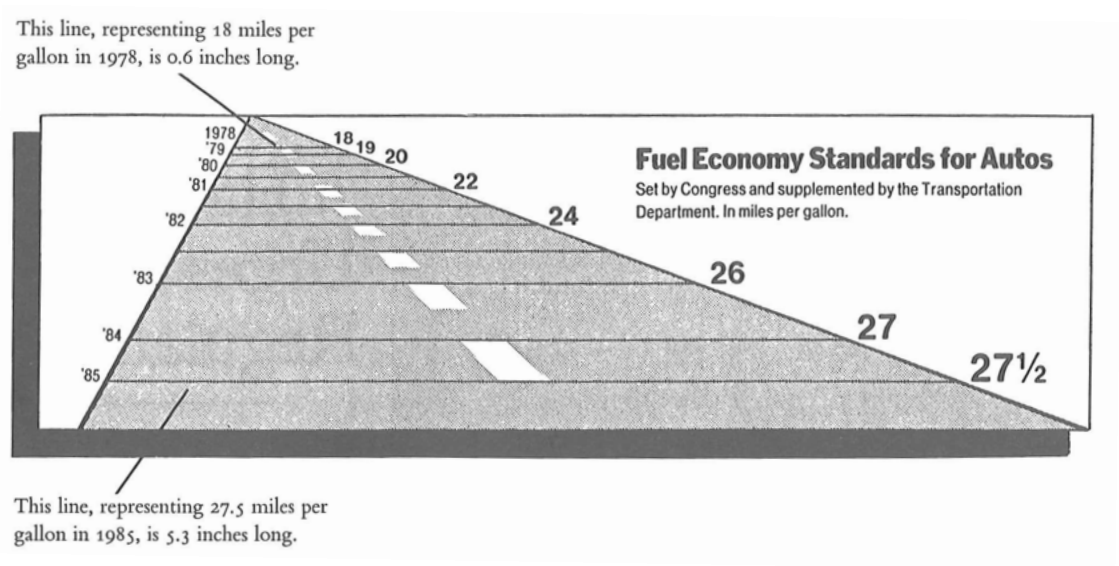
\includegraphics[keepaspectratio]{droga.png}}

{[}Tufte, 1991{]} Edward Tufte, The Visual Display of Quantitative
Information, Second Edition, Graphics Press, USA, 1991, p.~57 -- 69.

\[\operatorname{LieFactor} = \frac{\text{rozmiar efektu widocznego na wykresie}}{\text{rozmiar efektu wynikającego z danych}}\]

\[\text{rozmiar efektu} = \frac{|\text{druga wartość}-\text{pierwsza wartość}|}{\text{pierwsza wartość}}\]

\pandocbounded{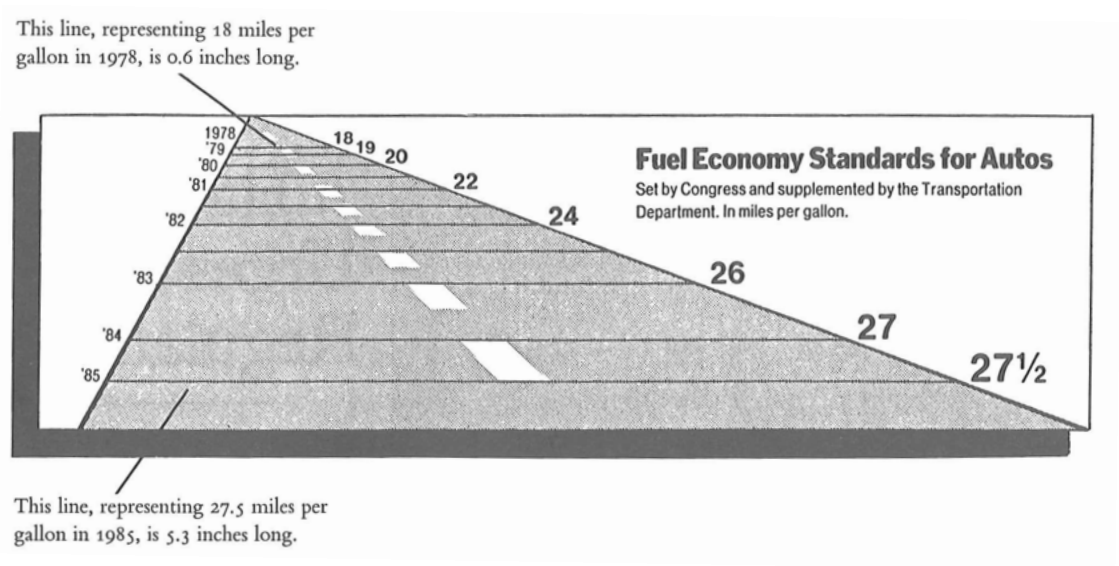
\includegraphics[keepaspectratio]{droga.png}}

\[\operatorname{LieFactor} = \frac{\frac{5.3-0.6}{0.6}}{\frac{27.5-18}{18}} \approx 14.8\]

\section{Bibliografia}\label{bibliografia-1}

\begin{itemize}
\tightlist
\item
  https://pl.wikipedia.org/wiki/Wizualizacja
\item
  https://mfiles.pl/pl/index.php/Analiza\_danych, dostęp online
  1.04.2019.
\item
  Walesiak M., Gatnar E., Statystyczna analiza danych z wykorzystaniem
  programu R, PWN, Warszawa, 2009.
\item
  Wasilewska E., Statystyka opisowa od podstaw, Podręcznik z zadaniami,
  Wydawnictwo SGGW, Warszawa, 2009.
\item
  https://en.wikipedia.org/wiki/Cognitive\_reflection\_test, dostęp
  online 20.03.2023.
\item
  https://qlikblog.pl/edward-tufte-dobre-praktyki-prezentacji-danych/,
  dostęp online 20.03.2023.
\end{itemize}

\part{NumPy}

\chapter{NumPy - start}\label{numpy---start}

NumPy jest biblioteką Pythona służącą do obliczeń naukowych.

Zastosowania:

\begin{itemize}
\tightlist
\item
  algebra liniowa
\item
  zaawansowane obliczenia matematyczne (numeryczne)
\item
  całkowania
\item
  rozwiązywanie równań
\item
  \ldots{}
\end{itemize}

\section{Instalacja pakietu NumPy - opcja łatwiejsza ``do
przeklikania''}\label{instalacja-pakietu-numpy---opcja-ux142atwiejsza-do-przeklikania}

\begin{itemize}
\tightlist
\item
  Tworzy projekt w PyCharm z venv - wersja 3.12.
\end{itemize}

\pandocbounded{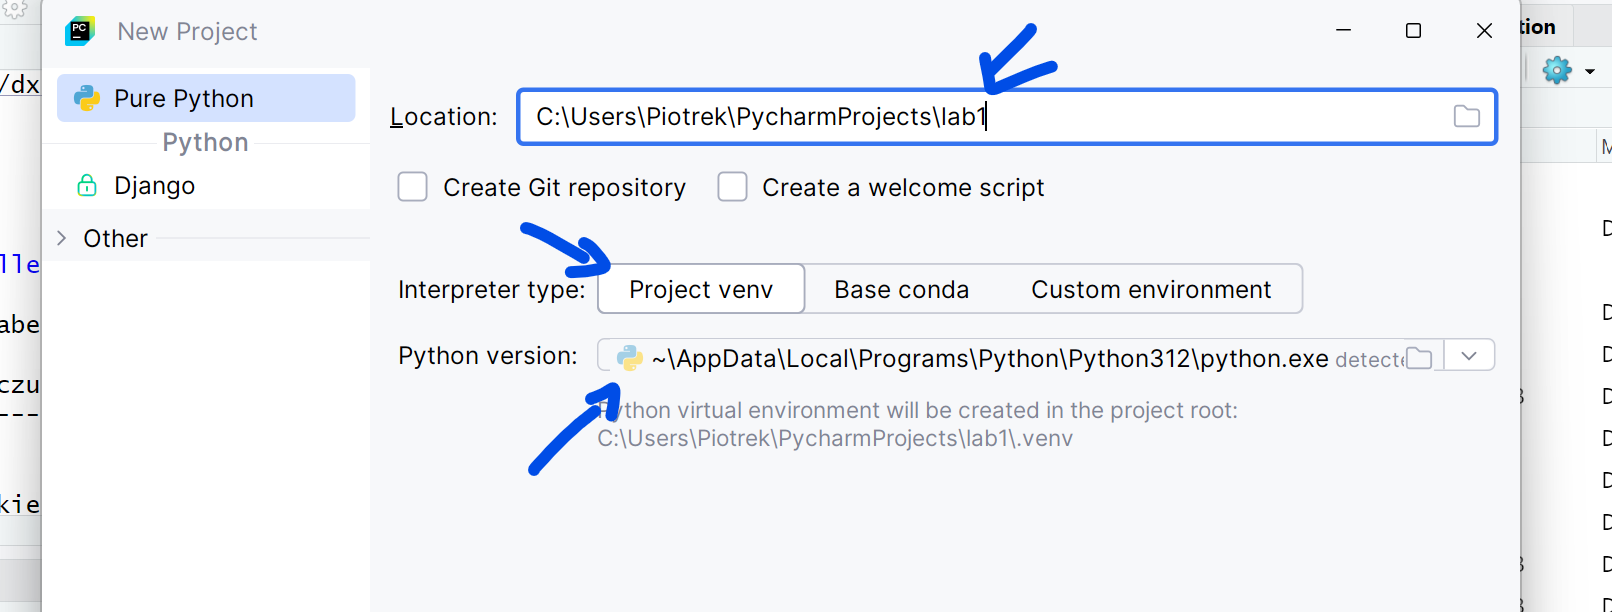
\includegraphics[keepaspectratio]{q1.png}}

\begin{itemize}
\tightlist
\item
  Za pomocą zakładki po lewej stronie na dole wyszukujemy pakiet i
  wybieramy instalację
\end{itemize}

\pandocbounded{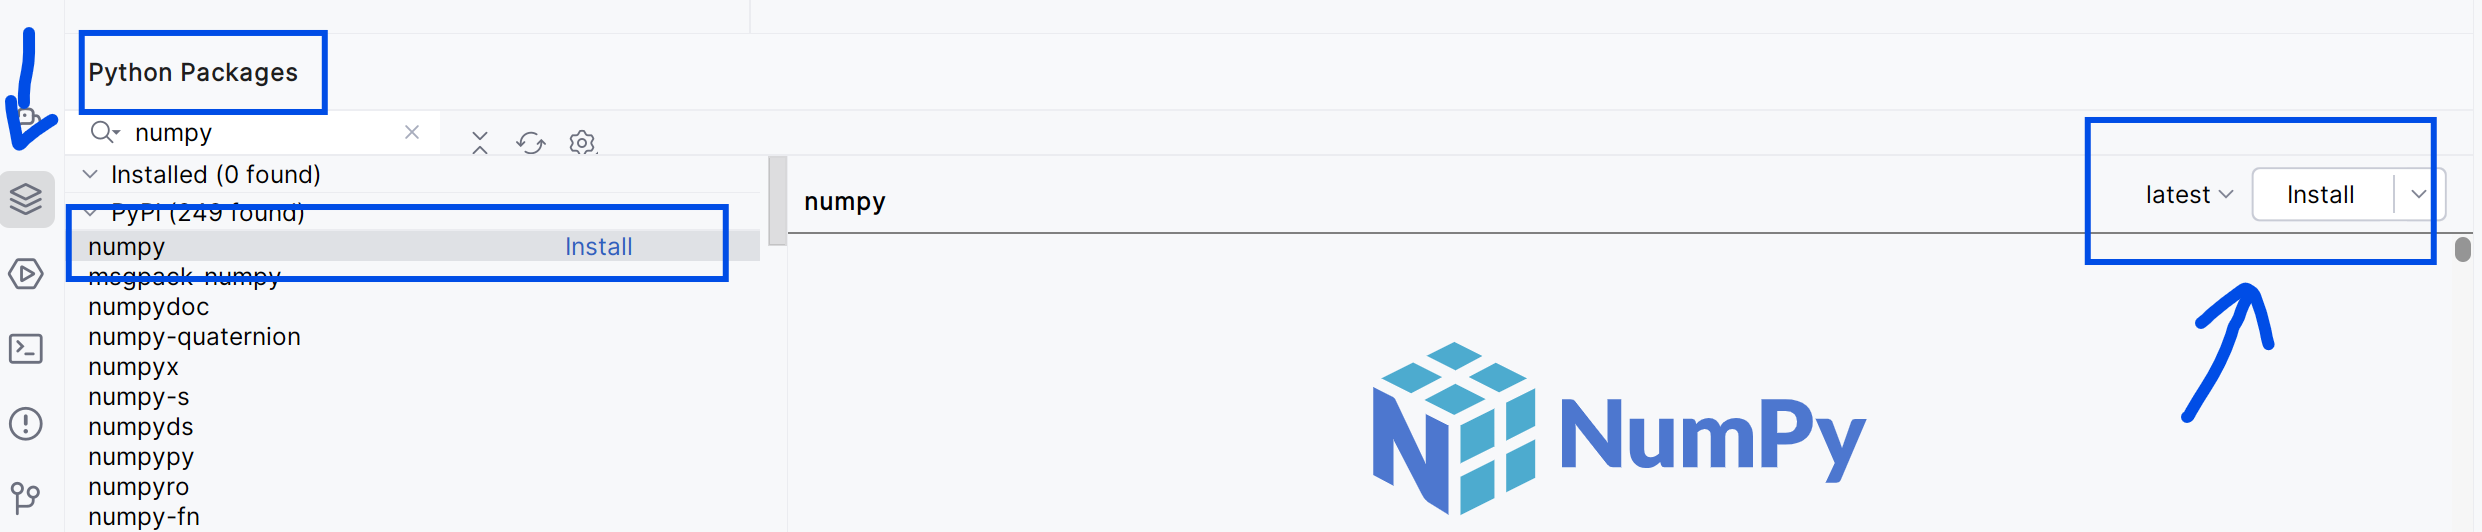
\includegraphics[keepaspectratio]{q2.png}}

\section{Instalacja pakietu NumPy - opcja
terminala}\label{instalacja-pakietu-numpy---opcja-terminala}

Komenda dla terminala:

\begin{Shaded}
\begin{Highlighting}[]
\ExtensionTok{python} \AttributeTok{{-}m}\NormalTok{ pip install numpy}
\end{Highlighting}
\end{Shaded}

\begin{Shaded}
\begin{Highlighting}[]
\ExtensionTok{python} \AttributeTok{{-}m}\NormalTok{ pip install numpy==2.2.0}
\end{Highlighting}
\end{Shaded}

\section{Import biblioteki NumPy}\label{import-biblioteki-numpy}

\begin{Shaded}
\begin{Highlighting}[]
\ImportTok{import}\NormalTok{ numpy }\ImportTok{as}\NormalTok{ np}
\end{Highlighting}
\end{Shaded}

Podstawowym bytem w bibliotece NumPy jest N-wymiarowa tablica zwana
\texttt{ndarray}. Każdy element na tablicy traktowany jest jako typ
\texttt{dtype}.

\begin{Shaded}
\begin{Highlighting}[]
\NormalTok{numpy.array(}\BuiltInTok{object}\NormalTok{, dtype}\OperatorTok{=}\VariableTok{None}\NormalTok{, }\OperatorTok{*}\NormalTok{, copy}\OperatorTok{=}\VariableTok{True}\NormalTok{, order}\OperatorTok{=}\StringTok{\textquotesingle{}K\textquotesingle{}}\NormalTok{, subok}\OperatorTok{=}\VariableTok{False}\NormalTok{, ndmin}\OperatorTok{=}\DecValTok{0}\NormalTok{, like}\OperatorTok{=}\VariableTok{None}\NormalTok{)}
\end{Highlighting}
\end{Shaded}

\begin{itemize}
\tightlist
\item
  object - to co ma być wrzucone do tablicy
\item
  dtype - typ
\item
  copy - czy obiekty mają być skopiowane, domyślne \texttt{True}
\item
  order - sposób układania: C (rzędy), F (kolumny), A, K
\item
  subok - realizowane przez podklasy (jeśli \texttt{True}), domyślnie
  \texttt{False}
\item
  ndmin - minimalny rozmiar (wymiar) tablicy
\item
  like - tworzenie na podstawie tablic referencyjnej
\end{itemize}

\phantomsection\label{annotated-cell-5}%
\begin{Shaded}
\begin{Highlighting}[]
\ImportTok{import}\NormalTok{ numpy }\ImportTok{as}\NormalTok{ np}

\NormalTok{a }\OperatorTok{=}\NormalTok{ np.array([}\DecValTok{1}\NormalTok{, }\DecValTok{2}\NormalTok{, }\DecValTok{3}\NormalTok{]) }\hspace*{\fill}\NormalTok{\circled{1}}
\BuiltInTok{print}\NormalTok{(}\StringTok{"a:"}\NormalTok{, a) }
\BuiltInTok{print}\NormalTok{(}\StringTok{"typ a:"}\NormalTok{, }\BuiltInTok{type}\NormalTok{(a)) }\hspace*{\fill}\NormalTok{\circled{2}}
\NormalTok{b }\OperatorTok{=}\NormalTok{ np.array([}\DecValTok{1}\NormalTok{, }\DecValTok{2}\NormalTok{, }\FloatTok{3.0}\NormalTok{]) }\hspace*{\fill}\NormalTok{\circled{3}}
\BuiltInTok{print}\NormalTok{(}\StringTok{"b:"}\NormalTok{, b)}
\NormalTok{c }\OperatorTok{=}\NormalTok{ np.array([[}\DecValTok{1}\NormalTok{, }\DecValTok{2}\NormalTok{], [}\DecValTok{3}\NormalTok{, }\DecValTok{4}\NormalTok{]]) }\hspace*{\fill}\NormalTok{\circled{4}}
\BuiltInTok{print}\NormalTok{(}\StringTok{"c:"}\NormalTok{, c)}
\NormalTok{d }\OperatorTok{=}\NormalTok{ np.array([}\DecValTok{1}\NormalTok{, }\DecValTok{2}\NormalTok{, }\DecValTok{3}\NormalTok{], ndmin}\OperatorTok{=}\DecValTok{2}\NormalTok{) }\hspace*{\fill}\NormalTok{\circled{5}}
\BuiltInTok{print}\NormalTok{(}\StringTok{"d:"}\NormalTok{, d)}
\NormalTok{e }\OperatorTok{=}\NormalTok{ np.array([}\DecValTok{1}\NormalTok{, }\DecValTok{2}\NormalTok{, }\DecValTok{3}\NormalTok{], dtype}\OperatorTok{=}\BuiltInTok{complex}\NormalTok{) }\hspace*{\fill}\NormalTok{\circled{6}}
\BuiltInTok{print}\NormalTok{(}\StringTok{"e:"}\NormalTok{, e)}
\NormalTok{f }\OperatorTok{=}\NormalTok{ np.array(np.asmatrix(}\StringTok{\textquotesingle{}1 2; 3 4\textquotesingle{}}\NormalTok{)) }\hspace*{\fill}\NormalTok{\circled{7}}
\BuiltInTok{print}\NormalTok{(}\StringTok{"f:"}\NormalTok{, f)}
\NormalTok{g }\OperatorTok{=}\NormalTok{ np.array(np.asmatrix(}\StringTok{\textquotesingle{}1 2; 3 4\textquotesingle{}}\NormalTok{), subok}\OperatorTok{=}\VariableTok{True}\NormalTok{) }\hspace*{\fill}\NormalTok{\circled{8}}
\BuiltInTok{print}\NormalTok{(}\StringTok{"g:"}\NormalTok{, g)}
\BuiltInTok{print}\NormalTok{(}\BuiltInTok{type}\NormalTok{(g))}
\end{Highlighting}
\end{Shaded}

\begin{description}
\tightlist
\item[\circled{1}]
Standardowe domyślne.
\item[\circled{2}]
Sprawdzenie typu.
\item[\circled{3}]
Jeden z elementów jest innego typu. Tu następuje zatem rozszerzenie do
typu ``największego''.
\item[\circled{4}]
Tu otrzymamy tablicę 2x2.
\item[\circled{5}]
W tej linijce otrzymana będzie tablica 2x1.
\item[\circled{6}]
Ustalenie innego typu - większego.
\item[\circled{7}]
Skorzystanie z podtypu macierzowego.
\item[\circled{8}]
Zachowanie typu macierzowego.
\end{description}

\begin{verbatim}
a: [1 2 3]
typ a: <class 'numpy.ndarray'>
b: [1. 2. 3.]
c: [[1 2]
 [3 4]]
d: [[1 2 3]]
e: [1.+0.j 2.+0.j 3.+0.j]
f: [[1 2]
 [3 4]]
g: [[1 2]
 [3 4]]
<class 'numpy.matrix'>
\end{verbatim}

\section{Uruchamianie - tryb ``Run''
(wykonawczy)}\label{uruchamianie---tryb-run-wykonawczy}

Run - zielona strzałka u góry.

\pandocbounded{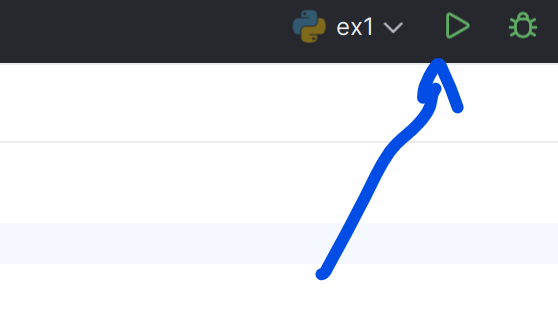
\includegraphics[keepaspectratio]{q3.png}}

\section{Uruchamianie - tryb ``Run in Python Console''
(interaktywno-wykonawczy)}\label{uruchamianie---tryb-run-in-python-console-interaktywno-wykonawczy}

\pandocbounded{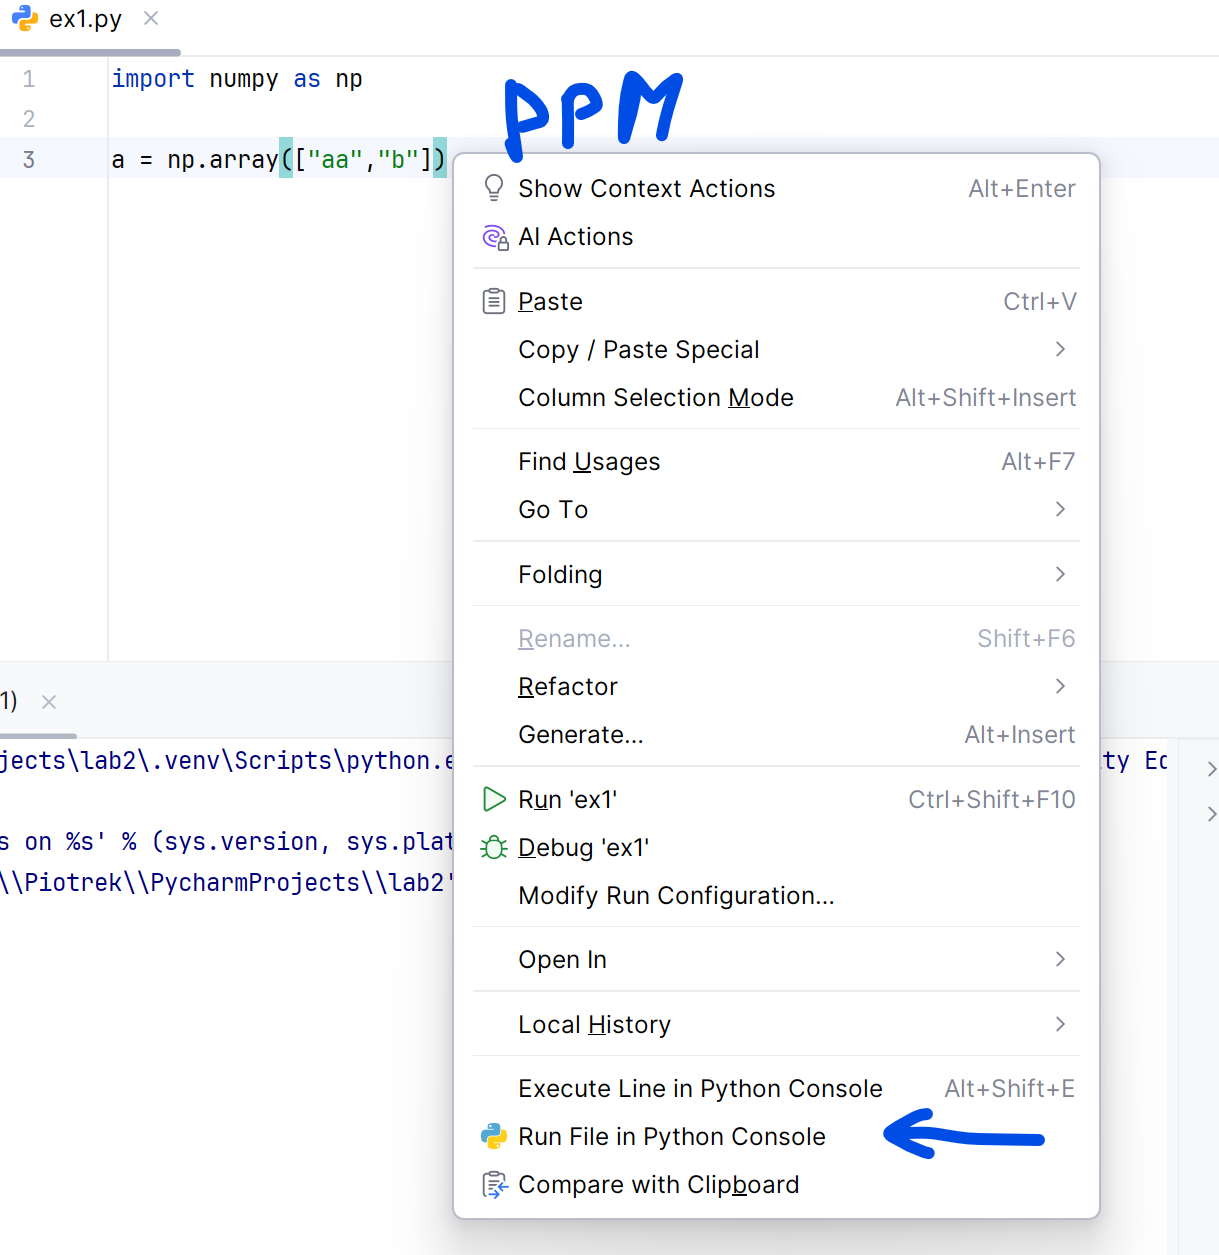
\includegraphics[keepaspectratio]{q4.png}}

\textbf{Ćwiczenie (\texttt{ex1.py}):}

\begin{enumerate}
\def\labelenumi{\arabic{enumi}.}
\tightlist
\item
  Stwórz proste tablice:
\end{enumerate}

\begin{itemize}
\item
  \(\begin{bmatrix}
  1 & 2 & 7\\
  6 & -3 & -3
  \end{bmatrix}\)
\item
  \(\begin{bmatrix}
  6 & 8 & 9 & -3
  \end{bmatrix}\)
\item
  \(\begin{bmatrix}
  4 \\ 3 \\-3 \\-7
  \end{bmatrix}\)
\item
  \(\begin{bmatrix}
  bb & cc & ww & 44
  \end{bmatrix}\)
\end{itemize}

\chapter{Lista a tablica}\label{lista-a-tablica}

\begin{Shaded}
\begin{Highlighting}[]
\ImportTok{import}\NormalTok{ numpy }\ImportTok{as}\NormalTok{ np}
\ImportTok{import}\NormalTok{ time}

\NormalTok{start\_time }\OperatorTok{=}\NormalTok{ time.time()}
\NormalTok{my\_arr }\OperatorTok{=}\NormalTok{ np.arange(}\DecValTok{1000000}\NormalTok{)}
\NormalTok{my\_list }\OperatorTok{=} \BuiltInTok{list}\NormalTok{(}\BuiltInTok{range}\NormalTok{(}\DecValTok{1000000}\NormalTok{))}
\NormalTok{start\_time }\OperatorTok{=}\NormalTok{ time.time()}
\NormalTok{my\_arr2 }\OperatorTok{=}\NormalTok{ my\_arr }\OperatorTok{*} \DecValTok{2}
\BuiltInTok{print}\NormalTok{(}\StringTok{"{-}{-}{-} }\SpecialCharTok{\%s}\StringTok{ seconds {-}{-}{-}"} \OperatorTok{\%}\NormalTok{ (time.time() }\OperatorTok{{-}}\NormalTok{ start\_time))}
\NormalTok{start\_time }\OperatorTok{=}\NormalTok{ time.time()}
\NormalTok{my\_list2 }\OperatorTok{=}\NormalTok{ [x }\OperatorTok{*} \DecValTok{2} \ControlFlowTok{for}\NormalTok{ x }\KeywordTok{in}\NormalTok{ my\_list]}
\BuiltInTok{print}\NormalTok{(}\StringTok{"{-}{-}{-} }\SpecialCharTok{\%s}\StringTok{ seconds {-}{-}{-}"} \OperatorTok{\%}\NormalTok{ (time.time() }\OperatorTok{{-}}\NormalTok{ start\_time))}
\end{Highlighting}
\end{Shaded}

\begin{verbatim}
--- 0.0017848014831542969 seconds ---
--- 0.03504204750061035 seconds ---
\end{verbatim}

\chapter{\texorpdfstring{Atrybuty tablic
\texttt{ndarray}}{Atrybuty tablic ndarray}}\label{atrybuty-tablic-ndarray}

\begin{longtable}[]{@{}
  >{\raggedright\arraybackslash}p{(\linewidth - 2\tabcolsep) * \real{0.5000}}
  >{\raggedright\arraybackslash}p{(\linewidth - 2\tabcolsep) * \real{0.5000}}@{}}
\toprule\noalign{}
\begin{minipage}[b]{\linewidth}\raggedright
Atrybut
\end{minipage} & \begin{minipage}[b]{\linewidth}\raggedright
Opis
\end{minipage} \\
\midrule\noalign{}
\endhead
\bottomrule\noalign{}
\endlastfoot
\texttt{shape} & krotka z informacją o liczbie elementów dla każdego z
wymiarów \\
\texttt{size} & liczba elementów w tablicy (łączna) \\
\texttt{ndim} & liczba wymiarów tablicy \\
\texttt{nbytes} & liczba bajtów jaką tablica zajmuje w pamięci \\
\texttt{dtype} & typ danych \\
\end{longtable}

\begin{Shaded}
\begin{Highlighting}[]
\ImportTok{import}\NormalTok{ numpy }\ImportTok{as}\NormalTok{ np}

\NormalTok{tab1 }\OperatorTok{=}\NormalTok{ np.array([}\DecValTok{2}\NormalTok{, }\OperatorTok{{-}}\DecValTok{3}\NormalTok{, }\DecValTok{4}\NormalTok{, }\OperatorTok{{-}}\DecValTok{8}\NormalTok{, }\DecValTok{1}\NormalTok{])}
\BuiltInTok{print}\NormalTok{(}\StringTok{"typ:"}\NormalTok{, }\BuiltInTok{type}\NormalTok{(tab1))}
\BuiltInTok{print}\NormalTok{(}\StringTok{"shape:"}\NormalTok{, tab1.shape)}
\BuiltInTok{print}\NormalTok{(}\StringTok{"size:"}\NormalTok{, tab1.size)}
\BuiltInTok{print}\NormalTok{(}\StringTok{"ndim:"}\NormalTok{, tab1.ndim)}
\BuiltInTok{print}\NormalTok{(}\StringTok{"nbytes:"}\NormalTok{, tab1.nbytes)}
\BuiltInTok{print}\NormalTok{(}\StringTok{"dtype:"}\NormalTok{, tab1.dtype)}
\end{Highlighting}
\end{Shaded}

\begin{verbatim}
typ: <class 'numpy.ndarray'>
shape: (5,)
size: 5
ndim: 1
nbytes: 40
dtype: int64
\end{verbatim}

\begin{Shaded}
\begin{Highlighting}[]
\ImportTok{import}\NormalTok{ numpy }\ImportTok{as}\NormalTok{ np}

\NormalTok{tab2 }\OperatorTok{=}\NormalTok{ np.array([[}\DecValTok{2}\NormalTok{, }\OperatorTok{{-}}\DecValTok{3}\NormalTok{], [}\DecValTok{4}\NormalTok{, }\OperatorTok{{-}}\DecValTok{8}\NormalTok{]])}
\BuiltInTok{print}\NormalTok{(}\StringTok{"typ:"}\NormalTok{, }\BuiltInTok{type}\NormalTok{(tab2))}
\BuiltInTok{print}\NormalTok{(}\StringTok{"shape:"}\NormalTok{, tab2.shape)}
\BuiltInTok{print}\NormalTok{(}\StringTok{"size:"}\NormalTok{, tab2.size)}
\BuiltInTok{print}\NormalTok{(}\StringTok{"ndim:"}\NormalTok{, tab2.ndim)}
\BuiltInTok{print}\NormalTok{(}\StringTok{"nbytes:"}\NormalTok{, tab2.nbytes)}
\BuiltInTok{print}\NormalTok{(}\StringTok{"dtype:"}\NormalTok{, tab2.dtype)}
\end{Highlighting}
\end{Shaded}

\begin{verbatim}
typ: <class 'numpy.ndarray'>
shape: (2, 2)
size: 4
ndim: 2
nbytes: 32
dtype: int64
\end{verbatim}

NumPy nie wspiera postrzępionych tablic! Poniższy kod wygeneruje błąd:

\begin{Shaded}
\begin{Highlighting}[]
\ImportTok{import}\NormalTok{ numpy }\ImportTok{as}\NormalTok{ np}

\NormalTok{tab3 }\OperatorTok{=}\NormalTok{ np.array([[}\DecValTok{2}\NormalTok{, }\OperatorTok{{-}}\DecValTok{3}\NormalTok{], [}\DecValTok{4}\NormalTok{, }\OperatorTok{{-}}\DecValTok{8}\NormalTok{, }\DecValTok{5}\NormalTok{], [}\DecValTok{3}\NormalTok{]])}
\end{Highlighting}
\end{Shaded}

\textbf{Ćwiczenia:} (\texttt{ex2.py})\\
Utwórz tablice numpy: \[
A = \begin{bmatrix} 1 & 2 & 3 \\ 4 & 5 & 6 \end{bmatrix}
\] \[B = \begin{bmatrix} 7 & 8 \\ 9 & 10 \\ 11 & 12 \end{bmatrix}\]
\[C = \begin{bmatrix} 1.1 & 2.2 & 3.3 \\ 4.4 & 5.5 & 6.6 \end{bmatrix}\]
i sprawdź ich parametry.

\chapter{Typy danych}\label{typy-danych}

\begin{longtable}[]{@{}
  >{\raggedright\arraybackslash}p{(\linewidth - 2\tabcolsep) * \real{0.5000}}
  >{\raggedright\arraybackslash}p{(\linewidth - 2\tabcolsep) * \real{0.5000}}@{}}
\toprule\noalign{}
\endhead
\bottomrule\noalign{}
\endlastfoot
Typy całkowitoliczbowe &
\texttt{int},\texttt{int8},\texttt{int16},\texttt{int32},\texttt{int64} \\
Typy całkowitoliczbowe (bez znaku) &
\texttt{uint},\texttt{uint8},\texttt{uint16},\texttt{uint32},\texttt{uint64} \\
Typ logiczny & \texttt{bool} \\
Typy zmiennoprzecinkowe & \texttt{float}, \texttt{float16},
\texttt{float32}, \texttt{float64}, \texttt{float128} \\
Typy zmiennoprzecinkowe zespolone & \texttt{complex},
\texttt{complex64}, \texttt{complex128}, \texttt{complex256} \\
Napis & \texttt{str} \\
\end{longtable}

\begin{Shaded}
\begin{Highlighting}[]
\ImportTok{import}\NormalTok{ numpy }\ImportTok{as}\NormalTok{ np}

\NormalTok{tab }\OperatorTok{=}\NormalTok{ np.array([[}\DecValTok{2}\NormalTok{, }\OperatorTok{{-}}\DecValTok{3}\NormalTok{], [}\DecValTok{4}\NormalTok{, }\OperatorTok{{-}}\DecValTok{8}\NormalTok{]])}
\BuiltInTok{print}\NormalTok{(tab)}
\NormalTok{tab2 }\OperatorTok{=}\NormalTok{ np.array([[}\DecValTok{2}\NormalTok{, }\OperatorTok{{-}}\DecValTok{3}\NormalTok{], [}\DecValTok{4}\NormalTok{, }\OperatorTok{{-}}\DecValTok{8}\NormalTok{]], dtype}\OperatorTok{=}\BuiltInTok{int}\NormalTok{)}
\BuiltInTok{print}\NormalTok{(tab2)}
\NormalTok{tab3 }\OperatorTok{=}\NormalTok{ np.array([[}\DecValTok{2}\NormalTok{, }\OperatorTok{{-}}\DecValTok{3}\NormalTok{], [}\DecValTok{4}\NormalTok{, }\OperatorTok{{-}}\DecValTok{8}\NormalTok{]], dtype}\OperatorTok{=}\BuiltInTok{float}\NormalTok{)}
\BuiltInTok{print}\NormalTok{(tab3)}
\NormalTok{tab4 }\OperatorTok{=}\NormalTok{ np.array([[}\DecValTok{2}\NormalTok{, }\OperatorTok{{-}}\DecValTok{3}\NormalTok{], [}\DecValTok{4}\NormalTok{, }\OperatorTok{{-}}\DecValTok{8}\NormalTok{]], dtype}\OperatorTok{=}\BuiltInTok{complex}\NormalTok{)}
\BuiltInTok{print}\NormalTok{(tab4)}
\end{Highlighting}
\end{Shaded}

\begin{verbatim}
[[ 2 -3]
 [ 4 -8]]
[[ 2 -3]
 [ 4 -8]]
[[ 2. -3.]
 [ 4. -8.]]
[[ 2.+0.j -3.+0.j]
 [ 4.+0.j -8.+0.j]]
\end{verbatim}

\chapter{Tworzenie tablic}\label{tworzenie-tablic}

\texttt{np.array} - argumenty rzutowany na tablicę (coś po czym można
iterować) - warto sprawdzić rozmiar/kształt

\begin{Shaded}
\begin{Highlighting}[]
\ImportTok{import}\NormalTok{ numpy }\ImportTok{as}\NormalTok{ np}

\NormalTok{tab }\OperatorTok{=}\NormalTok{ np.array([}\DecValTok{2}\NormalTok{, }\OperatorTok{{-}}\DecValTok{3}\NormalTok{, }\DecValTok{4}\NormalTok{])}
\BuiltInTok{print}\NormalTok{(tab)}
\BuiltInTok{print}\NormalTok{(}\StringTok{"size:"}\NormalTok{, tab.size)}
\NormalTok{tab2 }\OperatorTok{=}\NormalTok{ np.array((}\DecValTok{4}\NormalTok{, }\OperatorTok{{-}}\DecValTok{3}\NormalTok{, }\DecValTok{3}\NormalTok{, }\DecValTok{2}\NormalTok{))}
\BuiltInTok{print}\NormalTok{(tab2)}
\BuiltInTok{print}\NormalTok{(}\StringTok{"size:"}\NormalTok{, tab2.size)}
\NormalTok{tab3 }\OperatorTok{=}\NormalTok{ np.array(\{}\DecValTok{3}\NormalTok{, }\DecValTok{3}\NormalTok{, }\DecValTok{2}\NormalTok{, }\DecValTok{5}\NormalTok{, }\DecValTok{2}\NormalTok{\})}
\BuiltInTok{print}\NormalTok{(tab3)}
\BuiltInTok{print}\NormalTok{(}\StringTok{"size:"}\NormalTok{, tab3.size)}
\NormalTok{tab4 }\OperatorTok{=}\NormalTok{ np.array(\{}\StringTok{"pl"}\NormalTok{: }\DecValTok{344}\NormalTok{, }\StringTok{"en"}\NormalTok{: }\DecValTok{22}\NormalTok{\})}
\BuiltInTok{print}\NormalTok{(tab4)}
\BuiltInTok{print}\NormalTok{(}\StringTok{"size:"}\NormalTok{, tab4.size)}
\end{Highlighting}
\end{Shaded}

\begin{verbatim}
[ 2 -3  4]
size: 3
[ 4 -3  3  2]
size: 4
{2, 3, 5}
size: 1
{'pl': 344, 'en': 22}
size: 1
\end{verbatim}

\texttt{np.zeros} - tworzy tablicę wypełnioną zerami

\begin{Shaded}
\begin{Highlighting}[]
\ImportTok{import}\NormalTok{ numpy }\ImportTok{as}\NormalTok{ np}

\NormalTok{tab }\OperatorTok{=}\NormalTok{ np.zeros(}\DecValTok{4}\NormalTok{)}
\BuiltInTok{print}\NormalTok{(tab)}
\BuiltInTok{print}\NormalTok{(tab.shape)}
\NormalTok{tab2 }\OperatorTok{=}\NormalTok{ np.zeros([}\DecValTok{2}\NormalTok{, }\DecValTok{3}\NormalTok{])}
\BuiltInTok{print}\NormalTok{(tab2)}
\BuiltInTok{print}\NormalTok{(tab2.shape)}
\NormalTok{tab3 }\OperatorTok{=}\NormalTok{ np.zeros([}\DecValTok{2}\NormalTok{, }\DecValTok{3}\NormalTok{, }\DecValTok{4}\NormalTok{])}
\BuiltInTok{print}\NormalTok{(tab3)}
\BuiltInTok{print}\NormalTok{(tab3.shape)}
\end{Highlighting}
\end{Shaded}

\begin{verbatim}
[0. 0. 0. 0.]
(4,)
[[0. 0. 0.]
 [0. 0. 0.]]
(2, 3)
[[[0. 0. 0. 0.]
  [0. 0. 0. 0.]
  [0. 0. 0. 0.]]

 [[0. 0. 0. 0.]
  [0. 0. 0. 0.]
  [0. 0. 0. 0.]]]
(2, 3, 4)
\end{verbatim}

\texttt{np.ones} - tworzy tablicę wypełnioną jedynkami (to nie
odpowiednik macierzy jednostkowej!)

\begin{Shaded}
\begin{Highlighting}[]
\ImportTok{import}\NormalTok{ numpy }\ImportTok{as}\NormalTok{ np}

\NormalTok{tab }\OperatorTok{=}\NormalTok{ np.ones(}\DecValTok{4}\NormalTok{)}
\BuiltInTok{print}\NormalTok{(tab)}
\BuiltInTok{print}\NormalTok{(tab.shape)}
\NormalTok{tab2 }\OperatorTok{=}\NormalTok{ np.ones([}\DecValTok{2}\NormalTok{, }\DecValTok{3}\NormalTok{])}
\BuiltInTok{print}\NormalTok{(tab2)}
\BuiltInTok{print}\NormalTok{(tab2.shape)}
\NormalTok{tab3 }\OperatorTok{=}\NormalTok{ np.ones([}\DecValTok{2}\NormalTok{, }\DecValTok{3}\NormalTok{, }\DecValTok{4}\NormalTok{])}
\BuiltInTok{print}\NormalTok{(tab3)}
\BuiltInTok{print}\NormalTok{(tab3.shape)}
\end{Highlighting}
\end{Shaded}

\begin{verbatim}
[1. 1. 1. 1.]
(4,)
[[1. 1. 1.]
 [1. 1. 1.]]
(2, 3)
[[[1. 1. 1. 1.]
  [1. 1. 1. 1.]
  [1. 1. 1. 1.]]

 [[1. 1. 1. 1.]
  [1. 1. 1. 1.]
  [1. 1. 1. 1.]]]
(2, 3, 4)
\end{verbatim}

\texttt{np.diag} - tworzy tablicę odpowiadającą macierzy diagonalnej

\begin{Shaded}
\begin{Highlighting}[]
\ImportTok{import}\NormalTok{ numpy }\ImportTok{as}\NormalTok{ np}

\BuiltInTok{print}\NormalTok{(}\StringTok{"tab0"}\NormalTok{)}
\NormalTok{tab0 }\OperatorTok{=}\NormalTok{ np.diag([}\DecValTok{3}\NormalTok{, }\DecValTok{4}\NormalTok{, }\DecValTok{5}\NormalTok{])}
\BuiltInTok{print}\NormalTok{(tab0)}
\BuiltInTok{print}\NormalTok{(}\StringTok{"tab1"}\NormalTok{)}
\NormalTok{tab1 }\OperatorTok{=}\NormalTok{ np.array([[}\DecValTok{2}\NormalTok{, }\DecValTok{3}\NormalTok{, }\DecValTok{4}\NormalTok{], [}\DecValTok{3}\NormalTok{, }\OperatorTok{{-}}\DecValTok{4}\NormalTok{, }\DecValTok{5}\NormalTok{], [}\DecValTok{3}\NormalTok{, }\DecValTok{4}\NormalTok{, }\OperatorTok{{-}}\DecValTok{5}\NormalTok{]])}
\BuiltInTok{print}\NormalTok{(tab1)}
\NormalTok{tab2 }\OperatorTok{=}\NormalTok{ np.diag(tab1)}
\BuiltInTok{print}\NormalTok{(}\StringTok{"tab2"}\NormalTok{)}
\BuiltInTok{print}\NormalTok{(tab2)}
\NormalTok{tab3 }\OperatorTok{=}\NormalTok{ np.diag(tab1, k}\OperatorTok{=}\DecValTok{1}\NormalTok{)}
\BuiltInTok{print}\NormalTok{(}\StringTok{"tab3"}\NormalTok{)}
\BuiltInTok{print}\NormalTok{(tab3)}
\BuiltInTok{print}\NormalTok{(}\StringTok{"tab4"}\NormalTok{)}
\NormalTok{tab4 }\OperatorTok{=}\NormalTok{ np.diag(tab1, k}\OperatorTok{={-}}\DecValTok{2}\NormalTok{)}
\BuiltInTok{print}\NormalTok{(tab4)}
\BuiltInTok{print}\NormalTok{(}\StringTok{"tab5"}\NormalTok{)}
\NormalTok{tab5 }\OperatorTok{=}\NormalTok{ np.diag(np.diag(tab1))}
\BuiltInTok{print}\NormalTok{(tab5)}
\end{Highlighting}
\end{Shaded}

\begin{verbatim}
tab0
[[3 0 0]
 [0 4 0]
 [0 0 5]]
tab1
[[ 2  3  4]
 [ 3 -4  5]
 [ 3  4 -5]]
tab2
[ 2 -4 -5]
tab3
[3 5]
tab4
[3]
tab5
[[ 2  0  0]
 [ 0 -4  0]
 [ 0  0 -5]]
\end{verbatim}

\texttt{np.arange} - tablica wypełniona równomiernymi wartościami

Składnia:
\texttt{numpy.arange({[}start,\ {]}stop,\ {[}step,\ {]}dtype=None)}

Zasada działania jest podobna jak w funkcji \texttt{range}, ale
dopuszczamy liczby ``z ułamkiem''.

\begin{Shaded}
\begin{Highlighting}[]
\ImportTok{import}\NormalTok{ numpy }\ImportTok{as}\NormalTok{ np}

\NormalTok{a }\OperatorTok{=}\NormalTok{ np.arange(}\DecValTok{3}\NormalTok{)}
\BuiltInTok{print}\NormalTok{(a)}
\NormalTok{b }\OperatorTok{=}\NormalTok{ np.arange(}\FloatTok{3.0}\NormalTok{)}
\BuiltInTok{print}\NormalTok{(b)}
\NormalTok{c }\OperatorTok{=}\NormalTok{ np.arange(}\DecValTok{3}\NormalTok{, }\DecValTok{7}\NormalTok{)}
\BuiltInTok{print}\NormalTok{(c)}
\NormalTok{d }\OperatorTok{=}\NormalTok{ np.arange(}\DecValTok{3}\NormalTok{, }\DecValTok{11}\NormalTok{, }\DecValTok{2}\NormalTok{)}
\BuiltInTok{print}\NormalTok{(d)}
\NormalTok{e }\OperatorTok{=}\NormalTok{ np.arange(}\DecValTok{0}\NormalTok{, }\DecValTok{1}\NormalTok{, }\FloatTok{0.1}\NormalTok{)}
\BuiltInTok{print}\NormalTok{(e)}
\NormalTok{f }\OperatorTok{=}\NormalTok{ np.arange(}\DecValTok{3}\NormalTok{, }\DecValTok{11}\NormalTok{, }\DecValTok{2}\NormalTok{, dtype}\OperatorTok{=}\BuiltInTok{float}\NormalTok{)}
\BuiltInTok{print}\NormalTok{(f)}
\NormalTok{g }\OperatorTok{=}\NormalTok{ np.arange(}\DecValTok{3}\NormalTok{, }\DecValTok{10}\NormalTok{, }\DecValTok{2}\NormalTok{)}
\BuiltInTok{print}\NormalTok{(g)}
\end{Highlighting}
\end{Shaded}

\begin{verbatim}
[0 1 2]
[0. 1. 2.]
[3 4 5 6]
[3 5 7 9]
[0.  0.1 0.2 0.3 0.4 0.5 0.6 0.7 0.8 0.9]
[3. 5. 7. 9.]
[3 5 7 9]
\end{verbatim}

\texttt{np.linspace} - tablica wypełniona równomiernymi wartościami wg
skali liniowej

\begin{Shaded}
\begin{Highlighting}[]
\ImportTok{import}\NormalTok{ numpy }\ImportTok{as}\NormalTok{ np}

\NormalTok{a }\OperatorTok{=}\NormalTok{ np.linspace(}\FloatTok{2.0}\NormalTok{, }\FloatTok{3.0}\NormalTok{, num}\OperatorTok{=}\DecValTok{5}\NormalTok{)}
\BuiltInTok{print}\NormalTok{(a)}
\NormalTok{b }\OperatorTok{=}\NormalTok{ np.linspace(}\FloatTok{2.0}\NormalTok{, }\FloatTok{3.0}\NormalTok{, num}\OperatorTok{=}\DecValTok{5}\NormalTok{, endpoint}\OperatorTok{=}\VariableTok{False}\NormalTok{)}
\BuiltInTok{print}\NormalTok{(b)}
\NormalTok{c }\OperatorTok{=}\NormalTok{ np.linspace(}\DecValTok{10}\NormalTok{, }\DecValTok{20}\NormalTok{, num}\OperatorTok{=}\DecValTok{4}\NormalTok{)}
\BuiltInTok{print}\NormalTok{(c)}
\NormalTok{d }\OperatorTok{=}\NormalTok{ np.linspace(}\DecValTok{10}\NormalTok{, }\DecValTok{20}\NormalTok{, num}\OperatorTok{=}\DecValTok{4}\NormalTok{, dtype}\OperatorTok{=}\BuiltInTok{int}\NormalTok{)}
\BuiltInTok{print}\NormalTok{(d)}
\end{Highlighting}
\end{Shaded}

\begin{verbatim}
[2.   2.25 2.5  2.75 3.  ]
[2.  2.2 2.4 2.6 2.8]
[10.         13.33333333 16.66666667 20.        ]
[10 13 16 20]
\end{verbatim}

\pandocbounded{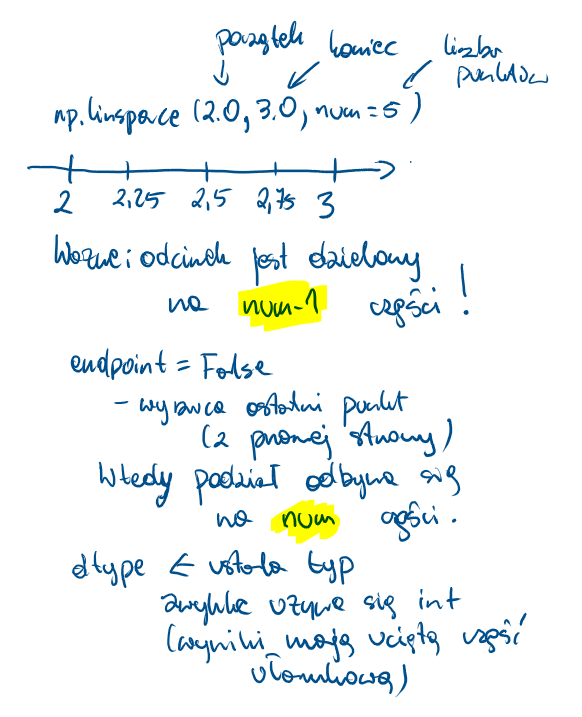
\includegraphics[keepaspectratio]{o1.png}}

\texttt{np.logspace} - tablica wypełniona wartościami wg skali
logarytmicznej

Składnia:
\texttt{numpy.logspace(start,\ stop,\ num=50,\ endpoint=True,\ base=10.0,\ dtype=None,\ axis=0)}

\begin{Shaded}
\begin{Highlighting}[]
\ImportTok{import}\NormalTok{ numpy }\ImportTok{as}\NormalTok{ np}

\NormalTok{a }\OperatorTok{=}\NormalTok{ np.logspace(}\FloatTok{2.0}\NormalTok{, }\FloatTok{3.0}\NormalTok{, num}\OperatorTok{=}\DecValTok{4}\NormalTok{)}
\BuiltInTok{print}\NormalTok{(a)}
\NormalTok{b }\OperatorTok{=}\NormalTok{ np.logspace(}\FloatTok{2.0}\NormalTok{, }\FloatTok{3.0}\NormalTok{, num}\OperatorTok{=}\DecValTok{4}\NormalTok{, endpoint}\OperatorTok{=}\VariableTok{False}\NormalTok{)}
\BuiltInTok{print}\NormalTok{(b)}
\NormalTok{c }\OperatorTok{=}\NormalTok{ np.logspace(}\FloatTok{2.0}\NormalTok{, }\FloatTok{3.0}\NormalTok{, num}\OperatorTok{=}\DecValTok{4}\NormalTok{, base}\OperatorTok{=}\FloatTok{2.0}\NormalTok{)}
\BuiltInTok{print}\NormalTok{(c)}
\end{Highlighting}
\end{Shaded}

\begin{verbatim}
[ 100.          215.443469    464.15888336 1000.        ]
[100.         177.827941   316.22776602 562.34132519]
[4.         5.0396842  6.34960421 8.        ]
\end{verbatim}

\pandocbounded{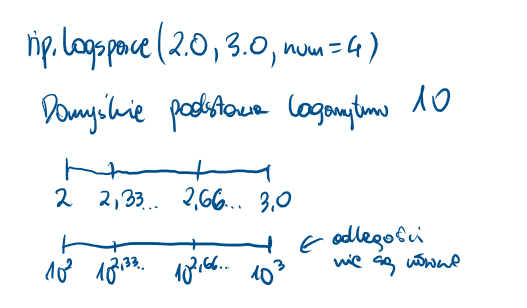
\includegraphics[keepaspectratio]{o2.png}}

\texttt{np.empty} - pusta (niezaincjowana) tablica - konkretne wartości
nie są ``gwarantowane''

\begin{Shaded}
\begin{Highlighting}[]
\ImportTok{import}\NormalTok{ numpy }\ImportTok{as}\NormalTok{ np}

\NormalTok{a }\OperatorTok{=}\NormalTok{ np.empty(}\DecValTok{3}\NormalTok{)}
\BuiltInTok{print}\NormalTok{(a)}
\NormalTok{b }\OperatorTok{=}\NormalTok{ np.empty(}\DecValTok{3}\NormalTok{, dtype}\OperatorTok{=}\BuiltInTok{int}\NormalTok{)}
\BuiltInTok{print}\NormalTok{(b)}
\end{Highlighting}
\end{Shaded}

\begin{verbatim}
[0. 1. 2.]
[                  0 4607182418800017408 4611686018427387904]
\end{verbatim}

\texttt{np.identity} - tablica przypominająca macierz jednostkową

\texttt{np.eye} - tablica z jedynkami na przekątnej (pozostałe zera)

\begin{Shaded}
\begin{Highlighting}[]
\ImportTok{import}\NormalTok{ numpy }\ImportTok{as}\NormalTok{ np}

\BuiltInTok{print}\NormalTok{(}\StringTok{"a"}\NormalTok{)}
\NormalTok{a }\OperatorTok{=}\NormalTok{ np.identity(}\DecValTok{4}\NormalTok{)}
\BuiltInTok{print}\NormalTok{(a)}
\BuiltInTok{print}\NormalTok{(}\StringTok{"b"}\NormalTok{)}
\NormalTok{b }\OperatorTok{=}\NormalTok{ np.eye(}\DecValTok{4}\NormalTok{, k}\OperatorTok{=}\DecValTok{1}\NormalTok{)}
\BuiltInTok{print}\NormalTok{(b)}
\BuiltInTok{print}\NormalTok{(}\StringTok{"c"}\NormalTok{)}
\NormalTok{c }\OperatorTok{=}\NormalTok{ np.eye(}\DecValTok{4}\NormalTok{, k}\OperatorTok{=}\DecValTok{2}\NormalTok{)}
\BuiltInTok{print}\NormalTok{(c)}
\BuiltInTok{print}\NormalTok{(}\StringTok{"d"}\NormalTok{)}
\NormalTok{d }\OperatorTok{=}\NormalTok{ np.eye(}\DecValTok{4}\NormalTok{, k}\OperatorTok{={-}}\DecValTok{1}\NormalTok{)}
\BuiltInTok{print}\NormalTok{(d)}
\end{Highlighting}
\end{Shaded}

\begin{verbatim}
a
[[1. 0. 0. 0.]
 [0. 1. 0. 0.]
 [0. 0. 1. 0.]
 [0. 0. 0. 1.]]
b
[[0. 1. 0. 0.]
 [0. 0. 1. 0.]
 [0. 0. 0. 1.]
 [0. 0. 0. 0.]]
c
[[0. 0. 1. 0.]
 [0. 0. 0. 1.]
 [0. 0. 0. 0.]
 [0. 0. 0. 0.]]
d
[[0. 0. 0. 0.]
 [1. 0. 0. 0.]
 [0. 1. 0. 0.]
 [0. 0. 1. 0.]]
\end{verbatim}

\textbf{Ćwiczenia:} (\texttt{ex3.py})

\begin{enumerate}
\def\labelenumi{\arabic{enumi}.}
\item
  Utwórz jednowymiarową tablicę zawierającą liczby całkowite od 1 do 5 i
  przypisz ją do zmiennej \texttt{A}. Wynikowa tablica powinna mieć
  postać: \[\begin{bmatrix}1 & 2 & 3 & 4 & 5\end{bmatrix} \]
\item
  Utwórz dwuwymiarową tablicę zawierającą elementy:
  \[\begin{bmatrix}1 & 2 \\ 3 & 4\end{bmatrix} \]\\
  i przypisz ją do zmiennej \texttt{B}.
\item
  Utwórz tablicę zawierającą liczby od 0 do 9 (włącznie). Przypisz ją do
  zmiennej \texttt{C}.\\
  Oczekiwana postać:
  \[\begin{bmatrix}0 & 1 & 2 & 3 & 4 & 5 & 6 & 7 & 8 & 9\end{bmatrix} \]
\item
  Utwórz tablicę zawierającą liczby od 10 do 30 z krokiem 5. Przypisz do
  \texttt{D}.\\
  Oczekiwana postać:
  \[\begin{bmatrix}10 & 15 & 20 & 25 & 30\end{bmatrix} \]
\item
  Utwórz tablicę 5 wartości równomiernie rozłożonych pomiędzy 0 a 1.
  Przypisz do \texttt{E}.\\
  Przykładowa postać:
  \[\begin{bmatrix}0. & 0.25 & 0.5 & 0.75 & 1.\end{bmatrix} \]
\item
  Utwórz dwuwymiarową tablicę o wymiarach 2x3 wypełnioną zerami.
  Przypisz do \texttt{F}.\\
  Oczekiwana postać:
  \[\begin{bmatrix}0 & 0 & 0 \\ 0 & 0 & 0\end{bmatrix} \]
\item
  Korzystając z \texttt{np.eye} utwórz macierz jednostkową 4x4. Przypisz
  do \texttt{J}.\\
  Oczekiwana postać:
  \[\begin{bmatrix}1 & 0 & 0 & 0 \\ 0 & 1 & 0 & 0 \\ 0 & 0 & 1 & 0 \\ 0 & 0 & 0 & 1\end{bmatrix} \]
\end{enumerate}

\chapter{Indeksowanie, ``krojenie''}\label{indeksowanie-krojenie}

\phantomsection\label{annotated-cell-20}%
\begin{Shaded}
\begin{Highlighting}[]
\ImportTok{import}\NormalTok{ numpy }\ImportTok{as}\NormalTok{ np}

\NormalTok{a }\OperatorTok{=}\NormalTok{ np.array([}\DecValTok{2}\NormalTok{, }\DecValTok{5}\NormalTok{, }\OperatorTok{{-}}\DecValTok{2}\NormalTok{, }\DecValTok{4}\NormalTok{, }\OperatorTok{{-}}\DecValTok{7}\NormalTok{, }\DecValTok{8}\NormalTok{, }\DecValTok{9}\NormalTok{, }\DecValTok{11}\NormalTok{, }\OperatorTok{{-}}\DecValTok{23}\NormalTok{, }\OperatorTok{{-}}\DecValTok{4}\NormalTok{, }\OperatorTok{{-}}\DecValTok{7}\NormalTok{, }\DecValTok{16}\NormalTok{, }\DecValTok{1}\NormalTok{])}
\BuiltInTok{print}\NormalTok{(}\StringTok{"1:"}\NormalTok{, a[}\DecValTok{5}\NormalTok{]) }\hspace*{\fill}\NormalTok{\circled{1}}
\BuiltInTok{print}\NormalTok{(}\StringTok{"2:"}\NormalTok{, a[}\OperatorTok{{-}}\DecValTok{2}\NormalTok{]) }\hspace*{\fill}\NormalTok{\circled{2}}
\BuiltInTok{print}\NormalTok{(}\StringTok{"3:"}\NormalTok{, a[}\DecValTok{3}\NormalTok{:}\DecValTok{6}\NormalTok{]) }\hspace*{\fill}\NormalTok{\circled{3}}
\BuiltInTok{print}\NormalTok{(}\StringTok{"4:"}\NormalTok{, a[:]) }\hspace*{\fill}\NormalTok{\circled{4}}
\BuiltInTok{print}\NormalTok{(}\StringTok{"5:"}\NormalTok{, a[}\DecValTok{0}\NormalTok{:}\OperatorTok{{-}}\DecValTok{1}\NormalTok{]) }\hspace*{\fill}\NormalTok{\circled{5}}
\BuiltInTok{print}\NormalTok{(}\StringTok{"6:"}\NormalTok{, a[:}\DecValTok{5}\NormalTok{]) }\hspace*{\fill}\NormalTok{\circled{6}}
\end{Highlighting}
\end{Shaded}

\begin{description}
\tightlist
\item[\circled{1}]
Dostęp do elementu o indeksie 5.
\item[\circled{2}]
Dostęp do elementu drugiego od tyłu.
\item[\circled{3}]
Dostęp do elementów o indeksach od 3 do 5 (włącznie) - zasada
przedziałów lewostronnnie domkniętnych, prawostronnie otwartych.
\item[\circled{4}]
Dostęp do wszystkich elementów.
\item[\circled{5}]
Dostęp do wszystkich elementów z wyłączeniem ostatniego.
\item[\circled{6}]
Dostęp od początku do elementu o indeksie 4.
\end{description}

\begin{verbatim}
1: 8
2: 16
3: [ 4 -7  8]
4: [  2   5  -2   4  -7   8   9  11 -23  -4  -7  16   1]
5: [  2   5  -2   4  -7   8   9  11 -23  -4  -7  16]
6: [ 2  5 -2  4 -7]
\end{verbatim}

\phantomsection\label{annotated-cell-21}%
\begin{Shaded}
\begin{Highlighting}[]
\ImportTok{import}\NormalTok{ numpy }\ImportTok{as}\NormalTok{ np}

\BuiltInTok{print}\NormalTok{(}\StringTok{"1:"}\NormalTok{, a[}\DecValTok{4}\NormalTok{:]) }\hspace*{\fill}\NormalTok{\circled{1}}
\BuiltInTok{print}\NormalTok{(}\StringTok{"2:"}\NormalTok{, a[}\DecValTok{4}\NormalTok{:}\OperatorTok{{-}}\DecValTok{1}\NormalTok{]) }\hspace*{\fill}\NormalTok{\circled{2}}
\BuiltInTok{print}\NormalTok{(}\StringTok{"3:"}\NormalTok{, a[}\DecValTok{4}\NormalTok{:}\DecValTok{10}\NormalTok{:}\DecValTok{2}\NormalTok{]) }\hspace*{\fill}\NormalTok{\circled{3}}
\BuiltInTok{print}\NormalTok{(}\StringTok{"4:"}\NormalTok{, a[::}\OperatorTok{{-}}\DecValTok{1}\NormalTok{]) }\hspace*{\fill}\NormalTok{\circled{4}}
\BuiltInTok{print}\NormalTok{(}\StringTok{"5:"}\NormalTok{, a[::}\DecValTok{2}\NormalTok{]) }\hspace*{\fill}\NormalTok{\circled{5}}
\BuiltInTok{print}\NormalTok{(}\StringTok{"6:"}\NormalTok{, a[::}\OperatorTok{{-}}\DecValTok{2}\NormalTok{]) }\hspace*{\fill}\NormalTok{\circled{6}}
\end{Highlighting}
\end{Shaded}

\begin{description}
\tightlist
\item[\circled{1}]
Dostęp do elementów od indeksu 4 do końca.
\item[\circled{2}]
Dostęp do elementów od indeksu 4 do końca bez ostatniego.
\item[\circled{3}]
Dostęp do elementów o indeksach stanowiących ciąg arytmetyczny od 4 do
10 (z czówrką, ale bez dziesiątki) z krokiem równym 2
\item[\circled{4}]
Dostęp do elementów od tyłu do początku.
\item[\circled{5}]
Dostęp do elementów o indeksach parzystych od początku.
\item[\circled{6}]
Dostęp do elementów o indeksach ``nieparzystych ujemnych'' od początku.
\end{description}

\begin{verbatim}
1: [ -7   8   9  11 -23  -4  -7  16   1]
2: [ -7   8   9  11 -23  -4  -7  16]
3: [ -7   9 -23]
4: [  1  16  -7  -4 -23  11   9   8  -7   4  -2   5   2]
5: [  2  -2  -7   9 -23  -7   1]
6: [  1  -7 -23   9  -7  -2   2]
\end{verbatim}

\begin{Shaded}
\begin{Highlighting}[]
\ImportTok{import}\NormalTok{ numpy }\ImportTok{as}\NormalTok{ np}

\NormalTok{a }\OperatorTok{=}\NormalTok{ np.array([[}\DecValTok{3}\NormalTok{, }\DecValTok{4}\NormalTok{, }\DecValTok{5}\NormalTok{], [}\OperatorTok{{-}}\DecValTok{3}\NormalTok{, }\DecValTok{4}\NormalTok{, }\DecValTok{8}\NormalTok{], [}\DecValTok{3}\NormalTok{, }\DecValTok{2}\NormalTok{, }\DecValTok{9}\NormalTok{]])}
\NormalTok{b }\OperatorTok{=}\NormalTok{ a[:}\DecValTok{2}\NormalTok{, }\DecValTok{1}\NormalTok{:]}
\BuiltInTok{print}\NormalTok{(b)}
\BuiltInTok{print}\NormalTok{(np.shape(b))}
\NormalTok{c }\OperatorTok{=}\NormalTok{ a[}\DecValTok{1}\NormalTok{]}
\BuiltInTok{print}\NormalTok{(c)}
\BuiltInTok{print}\NormalTok{(np.shape(c))}
\NormalTok{d }\OperatorTok{=}\NormalTok{ a[}\DecValTok{1}\NormalTok{, :]}
\BuiltInTok{print}\NormalTok{(d)}
\BuiltInTok{print}\NormalTok{(np.shape(d))}
\end{Highlighting}
\end{Shaded}

\begin{verbatim}
[[4 5]
 [4 8]]
(2, 2)
[-3  4  8]
(3,)
[-3  4  8]
(3,)
\end{verbatim}

\begin{Shaded}
\begin{Highlighting}[]
\ImportTok{import}\NormalTok{ numpy }\ImportTok{as}\NormalTok{ np}

\NormalTok{a }\OperatorTok{=}\NormalTok{ np.array([[}\DecValTok{3}\NormalTok{, }\DecValTok{4}\NormalTok{, }\DecValTok{5}\NormalTok{], [}\OperatorTok{{-}}\DecValTok{3}\NormalTok{, }\DecValTok{4}\NormalTok{, }\DecValTok{8}\NormalTok{], [}\DecValTok{3}\NormalTok{, }\DecValTok{2}\NormalTok{, }\DecValTok{9}\NormalTok{]])}
\NormalTok{e }\OperatorTok{=}\NormalTok{ a[}\DecValTok{1}\NormalTok{:}\DecValTok{2}\NormalTok{, :]}
\BuiltInTok{print}\NormalTok{(e)}
\BuiltInTok{print}\NormalTok{(np.shape(e))}
\NormalTok{f }\OperatorTok{=}\NormalTok{ a[:, :}\DecValTok{2}\NormalTok{]}
\BuiltInTok{print}\NormalTok{(f)}
\BuiltInTok{print}\NormalTok{(np.shape(f))}
\NormalTok{g }\OperatorTok{=}\NormalTok{ a[}\DecValTok{1}\NormalTok{, :}\DecValTok{2}\NormalTok{]}
\BuiltInTok{print}\NormalTok{(g)}
\BuiltInTok{print}\NormalTok{(np.shape(g))}
\NormalTok{h }\OperatorTok{=}\NormalTok{ a[}\DecValTok{1}\NormalTok{:}\DecValTok{2}\NormalTok{, :}\DecValTok{2}\NormalTok{]}
\BuiltInTok{print}\NormalTok{(h)}
\BuiltInTok{print}\NormalTok{(np.shape(h))}
\end{Highlighting}
\end{Shaded}

\begin{verbatim}
[[-3  4  8]]
(1, 3)
[[ 3  4]
 [-3  4]
 [ 3  2]]
(3, 2)
[-3  4]
(2,)
[[-3  4]]
(1, 2)
\end{verbatim}

**Uwaga - takie ``krojenie'' to tzw ``widok''.

\begin{Shaded}
\begin{Highlighting}[]
\ImportTok{import}\NormalTok{ numpy }\ImportTok{as}\NormalTok{ np}

\NormalTok{a }\OperatorTok{=}\NormalTok{ np.array([[}\DecValTok{3}\NormalTok{, }\DecValTok{4}\NormalTok{, }\DecValTok{5}\NormalTok{], [}\OperatorTok{{-}}\DecValTok{3}\NormalTok{, }\DecValTok{4}\NormalTok{, }\DecValTok{8}\NormalTok{], [}\DecValTok{3}\NormalTok{, }\DecValTok{2}\NormalTok{, }\DecValTok{9}\NormalTok{]])}
\NormalTok{b }\OperatorTok{=}\NormalTok{ a[}\DecValTok{1}\NormalTok{:}\DecValTok{2}\NormalTok{, }\DecValTok{1}\NormalTok{:]}
\BuiltInTok{print}\NormalTok{(b)}
\NormalTok{a[}\DecValTok{1}\NormalTok{][}\DecValTok{1}\NormalTok{] }\OperatorTok{=} \DecValTok{9}
\BuiltInTok{print}\NormalTok{(a)}
\BuiltInTok{print}\NormalTok{(b)}
\NormalTok{b[}\DecValTok{0}\NormalTok{][}\DecValTok{0}\NormalTok{] }\OperatorTok{=} \OperatorTok{{-}}\DecValTok{11}
\BuiltInTok{print}\NormalTok{(a)}
\BuiltInTok{print}\NormalTok{(b)}
\end{Highlighting}
\end{Shaded}

\begin{verbatim}
[[4 8]]
[[ 3  4  5]
 [-3  9  8]
 [ 3  2  9]]
[[9 8]]
[[  3   4   5]
 [ -3 -11   8]
 [  3   2   9]]
[[-11   8]]
\end{verbatim}

Naprawa:

\begin{Shaded}
\begin{Highlighting}[]
\ImportTok{import}\NormalTok{ numpy }\ImportTok{as}\NormalTok{ np}

\NormalTok{a }\OperatorTok{=}\NormalTok{ np.array([[}\DecValTok{3}\NormalTok{, }\DecValTok{4}\NormalTok{, }\DecValTok{5}\NormalTok{], [}\OperatorTok{{-}}\DecValTok{3}\NormalTok{, }\DecValTok{4}\NormalTok{, }\DecValTok{8}\NormalTok{], [}\DecValTok{3}\NormalTok{, }\DecValTok{2}\NormalTok{, }\DecValTok{9}\NormalTok{]])}
\NormalTok{b }\OperatorTok{=}\NormalTok{ a[}\DecValTok{1}\NormalTok{:}\DecValTok{2}\NormalTok{, }\DecValTok{1}\NormalTok{:].copy()}
\BuiltInTok{print}\NormalTok{(b)}
\NormalTok{a[}\DecValTok{1}\NormalTok{][}\DecValTok{1}\NormalTok{] }\OperatorTok{=} \DecValTok{9}
\BuiltInTok{print}\NormalTok{(a)}
\BuiltInTok{print}\NormalTok{(b)}
\NormalTok{b[}\DecValTok{0}\NormalTok{][}\DecValTok{0}\NormalTok{] }\OperatorTok{=} \OperatorTok{{-}}\DecValTok{11}
\BuiltInTok{print}\NormalTok{(a)}
\BuiltInTok{print}\NormalTok{(b)}
\end{Highlighting}
\end{Shaded}

\begin{verbatim}
[[4 8]]
[[ 3  4  5]
 [-3  9  8]
 [ 3  2  9]]
[[4 8]]
[[ 3  4  5]
 [-3  9  8]
 [ 3  2  9]]
[[-11   8]]
\end{verbatim}

Indeksowanie logiczne (fancy indexing, maski boolowskie)

\begin{Shaded}
\begin{Highlighting}[]
\ImportTok{import}\NormalTok{ numpy }\ImportTok{as}\NormalTok{ np}

\NormalTok{a }\OperatorTok{=}\NormalTok{ np.array([}\DecValTok{2}\NormalTok{, }\DecValTok{5}\NormalTok{, }\OperatorTok{{-}}\DecValTok{2}\NormalTok{, }\DecValTok{4}\NormalTok{, }\OperatorTok{{-}}\DecValTok{7}\NormalTok{, }\DecValTok{8}\NormalTok{, }\DecValTok{9}\NormalTok{, }\DecValTok{11}\NormalTok{, }\OperatorTok{{-}}\DecValTok{23}\NormalTok{, }\OperatorTok{{-}}\DecValTok{4}\NormalTok{, }\OperatorTok{{-}}\DecValTok{7}\NormalTok{, }\DecValTok{8}\NormalTok{, }\DecValTok{1}\NormalTok{])}
\NormalTok{b }\OperatorTok{=}\NormalTok{ a[np.array([}\DecValTok{1}\NormalTok{, }\DecValTok{3}\NormalTok{, }\DecValTok{7}\NormalTok{])]}
\BuiltInTok{print}\NormalTok{(b)}
\NormalTok{c }\OperatorTok{=}\NormalTok{ a[[}\DecValTok{1}\NormalTok{, }\DecValTok{3}\NormalTok{, }\DecValTok{7}\NormalTok{]]}
\BuiltInTok{print}\NormalTok{(c)}
\end{Highlighting}
\end{Shaded}

\begin{verbatim}
[ 5  4 11]
[ 5  4 11]
\end{verbatim}

\begin{Shaded}
\begin{Highlighting}[]
\ImportTok{import}\NormalTok{ numpy }\ImportTok{as}\NormalTok{ np}

\NormalTok{a }\OperatorTok{=}\NormalTok{ np.array([}\DecValTok{2}\NormalTok{, }\DecValTok{5}\NormalTok{, }\OperatorTok{{-}}\DecValTok{2}\NormalTok{, }\DecValTok{4}\NormalTok{, }\OperatorTok{{-}}\DecValTok{7}\NormalTok{, }\DecValTok{8}\NormalTok{, }\DecValTok{9}\NormalTok{, }\DecValTok{11}\NormalTok{, }\OperatorTok{{-}}\DecValTok{23}\NormalTok{, }\OperatorTok{{-}}\DecValTok{4}\NormalTok{, }\OperatorTok{{-}}\DecValTok{7}\NormalTok{, }\DecValTok{8}\NormalTok{, }\DecValTok{1}\NormalTok{])}
\NormalTok{b }\OperatorTok{=}\NormalTok{ a }\OperatorTok{\textgreater{}} \DecValTok{0}
\BuiltInTok{print}\NormalTok{(b)}
\NormalTok{c }\OperatorTok{=}\NormalTok{ a[a }\OperatorTok{\textgreater{}} \DecValTok{0}\NormalTok{]}
\BuiltInTok{print}\NormalTok{(c)}
\NormalTok{d }\OperatorTok{=}\NormalTok{ a[(a }\OperatorTok{\textgreater{}} \DecValTok{5}\NormalTok{) }\OperatorTok{\&}\NormalTok{ (a}\OperatorTok{\%}\DecValTok{2} \OperatorTok{!=}\DecValTok{0}\NormalTok{)] }\CommentTok{\# znak \& odpowiada za AND}
\BuiltInTok{print}\NormalTok{(d)}
\NormalTok{e }\OperatorTok{=}\NormalTok{ a[(a }\OperatorTok{\textgreater{}} \DecValTok{5}\NormalTok{) }\OperatorTok{|}\NormalTok{ (a}\OperatorTok{\%}\DecValTok{2} \OperatorTok{!=}\DecValTok{0}\NormalTok{)] }\CommentTok{\# znak | odpowiada za OR}
\BuiltInTok{print}\NormalTok{(e)}
\NormalTok{f }\OperatorTok{=}\NormalTok{ a[(a }\OperatorTok{\textgreater{}} \DecValTok{5}\NormalTok{) }\OperatorTok{\^{}}\NormalTok{ (a}\OperatorTok{\%}\DecValTok{2} \OperatorTok{!=}\DecValTok{0}\NormalTok{)] }\CommentTok{\# znak \^{} odpowiada za XOR}
\BuiltInTok{print}\NormalTok{(f)}
\NormalTok{g }\OperatorTok{=}\NormalTok{ a[}\OperatorTok{\textasciitilde{}}\NormalTok{(a }\OperatorTok{\textgreater{}} \DecValTok{0}\NormalTok{)]}
\BuiltInTok{print}\NormalTok{(g)}
\end{Highlighting}
\end{Shaded}

\begin{verbatim}
[ True  True False  True False  True  True  True False False False  True
  True]
[ 2  5  4  8  9 11  8  1]
[ 9 11]
[  5  -7   8   9  11 -23  -7   8   1]
[  5  -7   8 -23  -7   8   1]
[ -2  -7 -23  -4  -7]
\end{verbatim}

\begin{Shaded}
\begin{Highlighting}[]
\ImportTok{import}\NormalTok{ numpy }\ImportTok{as}\NormalTok{ np}

\NormalTok{a }\OperatorTok{=}\NormalTok{ np.array([}\DecValTok{2}\NormalTok{, }\DecValTok{5}\NormalTok{, }\OperatorTok{{-}}\DecValTok{2}\NormalTok{, }\DecValTok{4}\NormalTok{, }\OperatorTok{{-}}\DecValTok{7}\NormalTok{, }\DecValTok{8}\NormalTok{, }\DecValTok{9}\NormalTok{, }\DecValTok{11}\NormalTok{, }\OperatorTok{{-}}\DecValTok{23}\NormalTok{, }\OperatorTok{{-}}\DecValTok{4}\NormalTok{, }\OperatorTok{{-}}\DecValTok{7}\NormalTok{, }\DecValTok{8}\NormalTok{, }\DecValTok{1}\NormalTok{])}
\NormalTok{b }\OperatorTok{=}\NormalTok{ a[a }\OperatorTok{\textgreater{}} \DecValTok{0}\NormalTok{]}
\BuiltInTok{print}\NormalTok{(b)}
\NormalTok{b[}\DecValTok{0}\NormalTok{] }\OperatorTok{=} \OperatorTok{{-}}\DecValTok{5}
\BuiltInTok{print}\NormalTok{(a)}
\BuiltInTok{print}\NormalTok{(b)}
\NormalTok{a[}\DecValTok{1}\NormalTok{] }\OperatorTok{=} \DecValTok{20}
\BuiltInTok{print}\NormalTok{(a)}
\BuiltInTok{print}\NormalTok{(b)}
\end{Highlighting}
\end{Shaded}

\begin{verbatim}
[ 2  5  4  8  9 11  8  1]
[  2   5  -2   4  -7   8   9  11 -23  -4  -7   8   1]
[-5  5  4  8  9 11  8  1]
[  2  20  -2   4  -7   8   9  11 -23  -4  -7   8   1]
[-5  5  4  8  9 11  8  1]
\end{verbatim}

\textbf{Ćwiczenia:} (\texttt{ex4.py})

\begin{enumerate}
\def\labelenumi{\arabic{enumi}.}
\item
  Rozważ jednowymiarową tablicę\\
  \[A = \begin{bmatrix}10 & 20 & 30 & 40 & 50\end{bmatrix}.\]\\
  Napisz polecenie , które zwróci trzeci element tablicy. Następnie
  spróbuj pobrać przedział od drugiego do czwartego elementu włącznie.
\item
  Dla tej samej tablicy\\
  \[A = \begin{bmatrix}10 & 20 & 30 & 40 & 50\end{bmatrix},\]\\
  użyj ``fancy indexing'', aby wybrać elementy o indeksach
  \texttt{{[}0,\ 2,\ 4{]}}. Spróbuj także wykorzystać negatywne indeksy,
  aby wybrać ostatni i przedostatni element w jednej operacji.
\item
  Rozważ dwuwymiarową tablicę\\
  \[B = \begin{bmatrix}1 & 2 & 3 \\ 4 & 5 & 6 \\ 7 & 8 & 9\end{bmatrix}.\]\\
  Napisz polecenie, które zwróci drugi wiersz (jako tablicę
  jednowymiarową). Następnie pobierz cały pierwszy wiersz oraz dwie
  pierwsze kolumny.
\item
  Dla tablicy\\
  \[B = \begin{bmatrix}1 & 2 & 3 \\ 4 & 5 & 6 \\ 7 & 8 & 9\end{bmatrix},\]\\
  użyj ``fancy indexing'', aby wybrać elementy
  \((B_{1,1}, B_{0,2}, B_{2,0})\) za pomocą list indeksów w
  \texttt{numpy}. Otrzymaj wynik w postaci tablicy jednowymiarowej
  \texttt{{[}5,\ 3,\ 7{]}}.
\item
  Rozważ tablicę\\
  \[C = \begin{bmatrix}10 & 20 & 30 & 40 \\ 50 & 60 & 70 & 80\end{bmatrix}.\]\\
  Napisz polecenie, które zwróci wszystkie elementy drugiego wiersza
  oprócz ostatniego. Następnie pobierz co drugi element z pierwszego
  wiersza.
\item
  Dla tablicy\\
  \[C = \begin{bmatrix}10 & 20 & 30 & 40 \\ 50 & 60 & 70 & 80\end{bmatrix},\]\\
  użyj ``fancy indexing'', aby pobrać elementy pierwszego wiersza w
  kolejności \texttt{{[}30,\ 10,\ 40{]}} korzystając z tablicy indeksów
  np. \texttt{{[}2,\ 0,\ 3{]}}. Następnie zastosuj ``fancy indexing'' do
  drugiego wiersza, aby uzyskać \texttt{{[}80,\ 50{]}}.
\item
  Rozważ jednowymiarową tablicę\\
  \[D = \begin{bmatrix}5 & 10 & 15 & 20 & 25 & 30\end{bmatrix}.\]\\
  Za pomocą indeksowania wytnij ostatnie trzy elementy. Następnie
  pobierz wszystkie elementy o parzystych indeksach.
\item
  Dla tablicy\\
  \[D = \begin{bmatrix}5 & 10 & 15 & 20 & 25 & 30\end{bmatrix},\]\\
  użyj ``fancy indexing'' za pomocą maski boolowskiej (utwórz maskę
  wybierającą elementy większe niż 15) i otrzymaj odpowiednio
  przefiltrowaną tablicę. Następnie zastosuj tę maskę do pobrania
  konkretnych elementów.
\item
  Rozważ tablicę dwuwymiarową\\
  \[E = \begin{bmatrix}2 & 4 & 6 \\ 8 & 10 & 12 \\ 14 & 16 & 18\end{bmatrix}.\]\\
  Za pomocą indeksowania wybierz środkowy wiersz i wszystkie kolumny
  oprócz ostatniej. Następnie wybierz ostatni wiersz i ostatnią kolumnę.
\item
  Dla tablicy\\
  \[E = \begin{bmatrix}2 & 4 & 6 \\ 8 & 10 & 12 \\ 14 & 16 & 18\end{bmatrix},\]\\
  użyj ``fancy indexing'', aby w jednej operacji pobrać elementy
  \((E_{0,2}, E_{2,1})\) i ułożyć je w nowej tablicy. Spróbuj także
  stworzyć maskę boolowską wybierającą elementy większe niż 10 i pobrać
  wybrane wartości.
\end{enumerate}

\chapter{Modyfikacja kształtu i
rozmiaru}\label{modyfikacja-ksztaux142tu-i-rozmiaru}

\begin{Shaded}
\begin{Highlighting}[]
\ImportTok{import}\NormalTok{ numpy }\ImportTok{as}\NormalTok{ np}

\BuiltInTok{print}\NormalTok{(}\StringTok{"a"}\NormalTok{)}
\NormalTok{a }\OperatorTok{=}\NormalTok{ np.array([[}\DecValTok{3}\NormalTok{, }\DecValTok{4}\NormalTok{, }\DecValTok{5}\NormalTok{], [}\OperatorTok{{-}}\DecValTok{3}\NormalTok{, }\DecValTok{4}\NormalTok{, }\DecValTok{8}\NormalTok{], [}\DecValTok{3}\NormalTok{, }\DecValTok{2}\NormalTok{, }\DecValTok{9}\NormalTok{]])}
\BuiltInTok{print}\NormalTok{(a)}
\BuiltInTok{print}\NormalTok{(}\StringTok{"b"}\NormalTok{)}
\NormalTok{b }\OperatorTok{=}\NormalTok{ np.reshape(a, (}\DecValTok{1}\NormalTok{, }\DecValTok{9}\NormalTok{))}
\BuiltInTok{print}\NormalTok{(b)}
\BuiltInTok{print}\NormalTok{(}\StringTok{"c"}\NormalTok{)}
\NormalTok{c }\OperatorTok{=}\NormalTok{ a.reshape(}\DecValTok{9}\NormalTok{)}
\BuiltInTok{print}\NormalTok{(c)}
\end{Highlighting}
\end{Shaded}

\begin{verbatim}
a
[[ 3  4  5]
 [-3  4  8]
 [ 3  2  9]]
b
[[ 3  4  5 -3  4  8  3  2  9]]
c
[ 3  4  5 -3  4  8  3  2  9]
\end{verbatim}

\begin{Shaded}
\begin{Highlighting}[]
\ImportTok{import}\NormalTok{ numpy }\ImportTok{as}\NormalTok{ np}

\BuiltInTok{print}\NormalTok{(}\StringTok{"a"}\NormalTok{)}
\NormalTok{a }\OperatorTok{=}\NormalTok{ np.array([[}\DecValTok{3}\NormalTok{, }\DecValTok{4}\NormalTok{, }\DecValTok{5}\NormalTok{], [}\OperatorTok{{-}}\DecValTok{3}\NormalTok{, }\DecValTok{4}\NormalTok{, }\DecValTok{8}\NormalTok{], [}\DecValTok{3}\NormalTok{, }\DecValTok{2}\NormalTok{, }\DecValTok{9}\NormalTok{]])}
\BuiltInTok{print}\NormalTok{(a)}
\BuiltInTok{print}\NormalTok{(}\StringTok{"d"}\NormalTok{)}
\NormalTok{d }\OperatorTok{=}\NormalTok{ a.flatten()}
\BuiltInTok{print}\NormalTok{(d)}
\BuiltInTok{print}\NormalTok{(}\StringTok{"e"}\NormalTok{)}
\NormalTok{e }\OperatorTok{=}\NormalTok{ a.ravel()}
\BuiltInTok{print}\NormalTok{(e)}
\BuiltInTok{print}\NormalTok{(}\StringTok{"f"}\NormalTok{)}
\NormalTok{f }\OperatorTok{=}\NormalTok{ np.ravel(a)}
\BuiltInTok{print}\NormalTok{(f)}
\end{Highlighting}
\end{Shaded}

\begin{verbatim}
a
[[ 3  4  5]
 [-3  4  8]
 [ 3  2  9]]
d
[ 3  4  5 -3  4  8  3  2  9]
e
[ 3  4  5 -3  4  8  3  2  9]
f
[ 3  4  5 -3  4  8  3  2  9]
\end{verbatim}

\begin{Shaded}
\begin{Highlighting}[]
\ImportTok{import}\NormalTok{ numpy }\ImportTok{as}\NormalTok{ np}

\BuiltInTok{print}\NormalTok{(}\StringTok{"g"}\NormalTok{)}
\NormalTok{g }\OperatorTok{=}\NormalTok{ [[}\DecValTok{1}\NormalTok{, }\DecValTok{3}\NormalTok{, }\DecValTok{4}\NormalTok{]]}
\BuiltInTok{print}\NormalTok{(g)}
\BuiltInTok{print}\NormalTok{(}\StringTok{"h"}\NormalTok{)}
\NormalTok{h }\OperatorTok{=}\NormalTok{ np.squeeze(g)}
\BuiltInTok{print}\NormalTok{(h)}
\BuiltInTok{print}\NormalTok{(}\StringTok{"i"}\NormalTok{)}
\NormalTok{i }\OperatorTok{=}\NormalTok{ a.T}
\BuiltInTok{print}\NormalTok{(i)}
\BuiltInTok{print}\NormalTok{(}\StringTok{"j"}\NormalTok{)}
\NormalTok{j }\OperatorTok{=}\NormalTok{ np.transpose(a)}
\BuiltInTok{print}\NormalTok{(j)}
\end{Highlighting}
\end{Shaded}

\begin{verbatim}
g
[[1, 3, 4]]
h
[1 3 4]
i
[[ 3 -3  3]
 [ 4  4  2]
 [ 5  8  9]]
j
[[ 3 -3  3]
 [ 4  4  2]
 [ 5  8  9]]
\end{verbatim}

\begin{Shaded}
\begin{Highlighting}[]
\ImportTok{import}\NormalTok{ numpy }\ImportTok{as}\NormalTok{ np}

\BuiltInTok{print}\NormalTok{(}\StringTok{"h"}\NormalTok{)}
\NormalTok{h }\OperatorTok{=}\NormalTok{ [}\DecValTok{3}\NormalTok{, }\OperatorTok{{-}}\DecValTok{4}\NormalTok{, }\DecValTok{5}\NormalTok{, }\OperatorTok{{-}}\DecValTok{2}\NormalTok{]}
\BuiltInTok{print}\NormalTok{(h)}
\BuiltInTok{print}\NormalTok{(}\StringTok{"k"}\NormalTok{)}
\NormalTok{k }\OperatorTok{=}\NormalTok{ np.hstack((h, h, h))}
\BuiltInTok{print}\NormalTok{(k)}
\BuiltInTok{print}\NormalTok{(}\StringTok{"l"}\NormalTok{)}
\NormalTok{l }\OperatorTok{=}\NormalTok{ np.vstack((h, h, h))}
\BuiltInTok{print}\NormalTok{(l)}
\BuiltInTok{print}\NormalTok{(}\StringTok{"m"}\NormalTok{)}
\NormalTok{m }\OperatorTok{=}\NormalTok{ np.dstack((h, h, h))}
\BuiltInTok{print}\NormalTok{(m)}
\end{Highlighting}
\end{Shaded}

\begin{verbatim}
h
[3, -4, 5, -2]
k
[ 3 -4  5 -2  3 -4  5 -2  3 -4  5 -2]
l
[[ 3 -4  5 -2]
 [ 3 -4  5 -2]
 [ 3 -4  5 -2]]
m
[[[ 3  3  3]
  [-4 -4 -4]
  [ 5  5  5]
  [-2 -2 -2]]]
\end{verbatim}

\begin{Shaded}
\begin{Highlighting}[]
\ImportTok{import}\NormalTok{ numpy }\ImportTok{as}\NormalTok{ np}

\NormalTok{a }\OperatorTok{=}\NormalTok{ np.array([[}\DecValTok{1}\NormalTok{, }\DecValTok{2}\NormalTok{], [}\DecValTok{3}\NormalTok{, }\DecValTok{4}\NormalTok{]])}
\NormalTok{b }\OperatorTok{=}\NormalTok{ np.array([[}\DecValTok{5}\NormalTok{, }\DecValTok{6}\NormalTok{]])}
\BuiltInTok{print}\NormalTok{(}\StringTok{"r1"}\NormalTok{)}
\NormalTok{r1 }\OperatorTok{=}\NormalTok{ np.concatenate((a, b))}
\BuiltInTok{print}\NormalTok{(r1)}
\BuiltInTok{print}\NormalTok{(}\StringTok{"r2"}\NormalTok{)}
\NormalTok{r2 }\OperatorTok{=}\NormalTok{ np.concatenate((a, b), axis}\OperatorTok{=}\DecValTok{0}\NormalTok{)}
\BuiltInTok{print}\NormalTok{(r2)}
\BuiltInTok{print}\NormalTok{(}\StringTok{"r3"}\NormalTok{)}
\NormalTok{r3 }\OperatorTok{=}\NormalTok{ np.concatenate((a, b.T), axis}\OperatorTok{=}\DecValTok{1}\NormalTok{)}
\BuiltInTok{print}\NormalTok{(r3)}
\BuiltInTok{print}\NormalTok{(}\StringTok{"r4"}\NormalTok{)}
\NormalTok{r4 }\OperatorTok{=}\NormalTok{ np.concatenate((a, b), axis}\OperatorTok{=}\VariableTok{None}\NormalTok{)}
\BuiltInTok{print}\NormalTok{(r4)}
\end{Highlighting}
\end{Shaded}

\begin{verbatim}
r1
[[1 2]
 [3 4]
 [5 6]]
r2
[[1 2]
 [3 4]
 [5 6]]
r3
[[1 2 5]
 [3 4 6]]
r4
[1 2 3 4 5 6]
\end{verbatim}

\begin{Shaded}
\begin{Highlighting}[]
\ImportTok{import}\NormalTok{ numpy }\ImportTok{as}\NormalTok{ np}

\NormalTok{a }\OperatorTok{=}\NormalTok{ np.array([[}\DecValTok{1}\NormalTok{, }\DecValTok{2}\NormalTok{], [}\DecValTok{3}\NormalTok{, }\DecValTok{4}\NormalTok{]])}
\BuiltInTok{print}\NormalTok{(}\StringTok{"r1"}\NormalTok{)}
\NormalTok{r1 }\OperatorTok{=}\NormalTok{ np.resize(a, (}\DecValTok{2}\NormalTok{, }\DecValTok{3}\NormalTok{))}
\BuiltInTok{print}\NormalTok{(r1)}
\BuiltInTok{print}\NormalTok{(}\StringTok{"r2"}\NormalTok{)}
\NormalTok{r2 }\OperatorTok{=}\NormalTok{ np.resize(a, (}\DecValTok{1}\NormalTok{, }\DecValTok{4}\NormalTok{))}
\BuiltInTok{print}\NormalTok{(r2)}
\BuiltInTok{print}\NormalTok{(}\StringTok{"r3"}\NormalTok{)}
\NormalTok{r3 }\OperatorTok{=}\NormalTok{ np.resize(a, (}\DecValTok{2}\NormalTok{, }\DecValTok{4}\NormalTok{))}
\BuiltInTok{print}\NormalTok{(r3)}
\end{Highlighting}
\end{Shaded}

\begin{verbatim}
r1
[[1 2 3]
 [4 1 2]]
r2
[[1 2 3 4]]
r3
[[1 2 3 4]
 [1 2 3 4]]
\end{verbatim}

\begin{Shaded}
\begin{Highlighting}[]
\ImportTok{import}\NormalTok{ numpy }\ImportTok{as}\NormalTok{ np}

\NormalTok{a }\OperatorTok{=}\NormalTok{ np.array([[}\DecValTok{1}\NormalTok{, }\DecValTok{2}\NormalTok{], [}\DecValTok{3}\NormalTok{, }\DecValTok{4}\NormalTok{]])}
\NormalTok{b }\OperatorTok{=}\NormalTok{ np.array([[}\DecValTok{5}\NormalTok{, }\DecValTok{6}\NormalTok{]])}
\BuiltInTok{print}\NormalTok{(}\StringTok{"r1"}\NormalTok{)}
\NormalTok{r1 }\OperatorTok{=}\NormalTok{ np.append(a, b)}
\BuiltInTok{print}\NormalTok{(r1)}
\BuiltInTok{print}\NormalTok{(}\StringTok{"r2"}\NormalTok{)}
\NormalTok{r2 }\OperatorTok{=}\NormalTok{ np.append(a, b, axis}\OperatorTok{=}\DecValTok{0}\NormalTok{)}
\BuiltInTok{print}\NormalTok{(r2)}
\end{Highlighting}
\end{Shaded}

\begin{verbatim}
r1
[1 2 3 4 5 6]
r2
[[1 2]
 [3 4]
 [5 6]]
\end{verbatim}

\begin{Shaded}
\begin{Highlighting}[]
\ImportTok{import}\NormalTok{ numpy }\ImportTok{as}\NormalTok{ np}

\NormalTok{a }\OperatorTok{=}\NormalTok{ np.array([[}\DecValTok{1}\NormalTok{, }\DecValTok{2}\NormalTok{], [}\DecValTok{3}\NormalTok{, }\DecValTok{7}\NormalTok{]])}
\BuiltInTok{print}\NormalTok{(}\StringTok{"r1"}\NormalTok{)}
\NormalTok{r1 }\OperatorTok{=}\NormalTok{ np.insert(a, }\DecValTok{1}\NormalTok{, }\DecValTok{4}\NormalTok{)}
\BuiltInTok{print}\NormalTok{(r1)}
\BuiltInTok{print}\NormalTok{(}\StringTok{"r2"}\NormalTok{)}
\NormalTok{r2 }\OperatorTok{=}\NormalTok{ np.insert(a, }\DecValTok{2}\NormalTok{, }\DecValTok{4}\NormalTok{)}
\BuiltInTok{print}\NormalTok{(r2)}
\BuiltInTok{print}\NormalTok{(}\StringTok{"r3"}\NormalTok{)}
\NormalTok{r3 }\OperatorTok{=}\NormalTok{ np.insert(a, }\DecValTok{1}\NormalTok{, }\DecValTok{4}\NormalTok{, axis}\OperatorTok{=}\DecValTok{0}\NormalTok{)}
\BuiltInTok{print}\NormalTok{(r3)}
\BuiltInTok{print}\NormalTok{(}\StringTok{"r4"}\NormalTok{)}
\NormalTok{r4 }\OperatorTok{=}\NormalTok{ np.insert(a, }\DecValTok{1}\NormalTok{, }\DecValTok{4}\NormalTok{, axis}\OperatorTok{=}\DecValTok{1}\NormalTok{)}
\BuiltInTok{print}\NormalTok{(r4)}
\end{Highlighting}
\end{Shaded}

\begin{verbatim}
r1
[1 4 2 3 7]
r2
[1 2 4 3 7]
r3
[[1 2]
 [4 4]
 [3 7]]
r4
[[1 4 2]
 [3 4 7]]
\end{verbatim}

\begin{Shaded}
\begin{Highlighting}[]
\ImportTok{import}\NormalTok{ numpy }\ImportTok{as}\NormalTok{ np}

\NormalTok{a }\OperatorTok{=}\NormalTok{ np.array([[}\DecValTok{1}\NormalTok{, }\DecValTok{2}\NormalTok{, }\DecValTok{3}\NormalTok{, }\DecValTok{4}\NormalTok{], [}\DecValTok{5}\NormalTok{, }\DecValTok{6}\NormalTok{, }\DecValTok{7}\NormalTok{, }\DecValTok{8}\NormalTok{], [}\DecValTok{9}\NormalTok{, }\DecValTok{10}\NormalTok{, }\DecValTok{11}\NormalTok{, }\DecValTok{12}\NormalTok{]])}
\BuiltInTok{print}\NormalTok{(}\StringTok{"r1"}\NormalTok{)}
\NormalTok{r1 }\OperatorTok{=}\NormalTok{ np.delete(a, }\DecValTok{1}\NormalTok{, axis}\OperatorTok{=}\DecValTok{1}\NormalTok{)}
\BuiltInTok{print}\NormalTok{(r1)}
\BuiltInTok{print}\NormalTok{(}\StringTok{"r2"}\NormalTok{)}
\NormalTok{r2 }\OperatorTok{=}\NormalTok{ np.delete(a, }\DecValTok{2}\NormalTok{, axis}\OperatorTok{=}\DecValTok{0}\NormalTok{)}
\BuiltInTok{print}\NormalTok{(r2)}
\end{Highlighting}
\end{Shaded}

\begin{verbatim}
r1
[[ 1  3  4]
 [ 5  7  8]
 [ 9 11 12]]
r2
[[1 2 3 4]
 [5 6 7 8]]
\end{verbatim}

\textbf{Ćwiczenia:} (\texttt{ex5.py})

\begin{enumerate}
\def\labelenumi{\arabic{enumi}.}
\item
  Rozważ tablicę jednowymiarową\\
  \[A = \begin{bmatrix}1 & 2 & 3 & 4 & 5 & 6\end{bmatrix}.\]\\
  Przekształć ją tak, aby uzyskać tablicę dwuwymiarową o kształcie
  \(2 \times 3\).
\item
  Mając tablicę dwuwymiarową\\
  \[B = \begin{bmatrix}1 & 2 \\ 3 & 4 \\ 5 & 6\end{bmatrix},\]\\
  uzyskaj jednowymiarowy ``widok'' jej elementów bez zmiany w danych
  źródłowych.
\item
  Rozważ tablicę\\
  \[D = \begin{bmatrix}1 & 2 & 3 \\ 4 & 5 & 6\end{bmatrix}.\]\\
  Zmień jej orientację tak, aby wiersze stały się kolumnami, a kolumny
  wierszami.
\item
  Mając dwie tablice\\
  \[E_1 = \begin{bmatrix}1 & 2 & 3\end{bmatrix}, \quad E_2 = \begin{bmatrix}4 & 5 & 6\end{bmatrix},\]\\
  połącz je w poziomie, tworząc jedną tablicę.
\item
  Dwie tablice\\
  \[F_1 = \begin{bmatrix}1 & 2 & 3\end{bmatrix}, \quad F_2 = \begin{bmatrix}4 & 5 & 6\end{bmatrix},\]\\
  połącz w pionie, aby uzyskać tablicę o kształcie \(2 \times 3\).
\item
  Dla tablicy\\
  \[G = \begin{bmatrix}1 & 2 & 3 \\ 4 & 5 & 6\end{bmatrix},\]\\
  zmień jej rozmiar tak, aby stała się tablicą jednowymiarową o 4
  elementach. Pozostałe elementy usuń.
\item
  Mając tablicę\\
  \[H = \begin{bmatrix}10 & 20 & 30 \\ 40 & 50 & 60 \\ 70 & 80 & 90\end{bmatrix},\]\\
  usuń drugą kolumnę, otrzymując tablicę \(3 \times 2\).
\item
  Rozważ tablicę\\
  \[I = \begin{bmatrix}1 & 2 \\ 3 & 4 \\ 5 & 6 \\ 7 & 8\end{bmatrix},\]\\
  zmień jej kształt tak, aby uzyskać tablicę \(2 \times 4\).
\item
  Mając tablicę\\
  \[J = \begin{bmatrix}1 & 2 & 3 & 4\end{bmatrix},\]\\
  przekształć ją w tablicę dwuwymiarową \(2 \times 2\), a następnie
  ``spłaszcz'' ją z powrotem do postaci jednowymiarowej.
\end{enumerate}

\chapter{Broadcasting}\label{broadcasting}

Rozważane warianty są przykładowe.

Wariant 1 - skalar-tablica - wykonanie operacji na każdym elemencie
tablicy

\begin{Shaded}
\begin{Highlighting}[]
\ImportTok{import}\NormalTok{ numpy }\ImportTok{as}\NormalTok{ np}

\NormalTok{a }\OperatorTok{=}\NormalTok{ np.array([[}\DecValTok{1}\NormalTok{, }\DecValTok{2}\NormalTok{], [}\DecValTok{5}\NormalTok{, }\DecValTok{6}\NormalTok{], [}\DecValTok{9}\NormalTok{, }\DecValTok{10}\NormalTok{]])}
\NormalTok{b }\OperatorTok{=}\NormalTok{ a }\OperatorTok{+} \DecValTok{4}
\BuiltInTok{print}\NormalTok{(b)}
\NormalTok{c }\OperatorTok{=} \DecValTok{2} \OperatorTok{**}\NormalTok{ a}
\BuiltInTok{print}\NormalTok{(c)}
\end{Highlighting}
\end{Shaded}

\begin{verbatim}
[[ 5  6]
 [ 9 10]
 [13 14]]
[[   2    4]
 [  32   64]
 [ 512 1024]]
\end{verbatim}

\pandocbounded{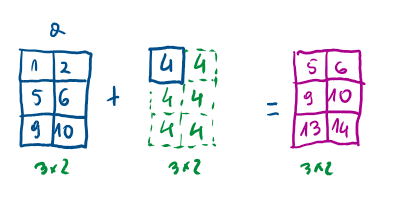
\includegraphics[keepaspectratio]{o3.png}}

Wariant 2 - dwie tablice - ``gdy jedna z tablic może być rozszerzona''
(oba wymiary są równe lub jeden z nich jest równy 1)

\begin{Shaded}
\begin{Highlighting}[]
\ImportTok{import}\NormalTok{ numpy }\ImportTok{as}\NormalTok{ np}

\NormalTok{a }\OperatorTok{=}\NormalTok{ np.array([[}\DecValTok{1}\NormalTok{, }\DecValTok{2}\NormalTok{], [}\DecValTok{5}\NormalTok{, }\DecValTok{6}\NormalTok{]])}
\NormalTok{b }\OperatorTok{=}\NormalTok{ np.array([}\DecValTok{9}\NormalTok{, }\DecValTok{2}\NormalTok{])}
\NormalTok{r1 }\OperatorTok{=}\NormalTok{ a }\OperatorTok{+}\NormalTok{ b}
\BuiltInTok{print}\NormalTok{(r1)}
\NormalTok{r2 }\OperatorTok{=}\NormalTok{ a }\OperatorTok{/}\NormalTok{ b}
\BuiltInTok{print}\NormalTok{(r2)}
\NormalTok{c }\OperatorTok{=}\NormalTok{ np.array([[}\DecValTok{4}\NormalTok{], [}\OperatorTok{{-}}\DecValTok{2}\NormalTok{]])}
\NormalTok{r3 }\OperatorTok{=}\NormalTok{ a }\OperatorTok{+}\NormalTok{ c}
\BuiltInTok{print}\NormalTok{(r3)}
\NormalTok{r4 }\OperatorTok{=}\NormalTok{ c }\OperatorTok{/}\NormalTok{ a}
\BuiltInTok{print}\NormalTok{(r4)}
\end{Highlighting}
\end{Shaded}

\begin{verbatim}
[[10  4]
 [14  8]]
[[0.11111111 1.        ]
 [0.55555556 3.        ]]
[[5 6]
 [3 4]]
[[ 4.          2.        ]
 [-0.4        -0.33333333]]
\end{verbatim}

\pandocbounded{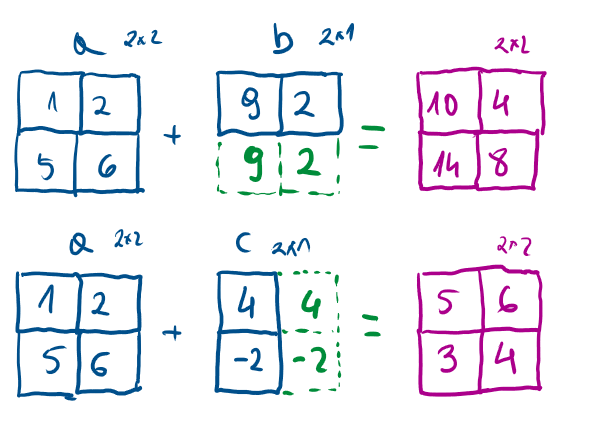
\includegraphics[keepaspectratio]{a4.png}}

Wariant 3 - ``kolumna'' i ``wiersz''

\begin{Shaded}
\begin{Highlighting}[]
\ImportTok{import}\NormalTok{ numpy }\ImportTok{as}\NormalTok{ np}

\NormalTok{a }\OperatorTok{=}\NormalTok{ np.array([[}\DecValTok{5}\NormalTok{, }\DecValTok{2}\NormalTok{, }\OperatorTok{{-}}\DecValTok{3}\NormalTok{]]).T}
\NormalTok{b }\OperatorTok{=}\NormalTok{ np.array([}\DecValTok{3}\NormalTok{, }\OperatorTok{{-}}\DecValTok{2}\NormalTok{, }\DecValTok{1}\NormalTok{, }\DecValTok{2}\NormalTok{, }\DecValTok{4}\NormalTok{])}
\BuiltInTok{print}\NormalTok{(a}\OperatorTok{+}\NormalTok{b)}
\BuiltInTok{print}\NormalTok{(b}\OperatorTok{+}\NormalTok{a)}
\BuiltInTok{print}\NormalTok{(a}\OperatorTok{*}\NormalTok{b)}
\end{Highlighting}
\end{Shaded}

\begin{verbatim}
[[ 8  3  6  7  9]
 [ 5  0  3  4  6]
 [ 0 -5 -2 -1  1]]
[[ 8  3  6  7  9]
 [ 5  0  3  4  6]
 [ 0 -5 -2 -1  1]]
[[ 15 -10   5  10  20]
 [  6  -4   2   4   8]
 [ -9   6  -3  -6 -12]]
\end{verbatim}

\pandocbounded{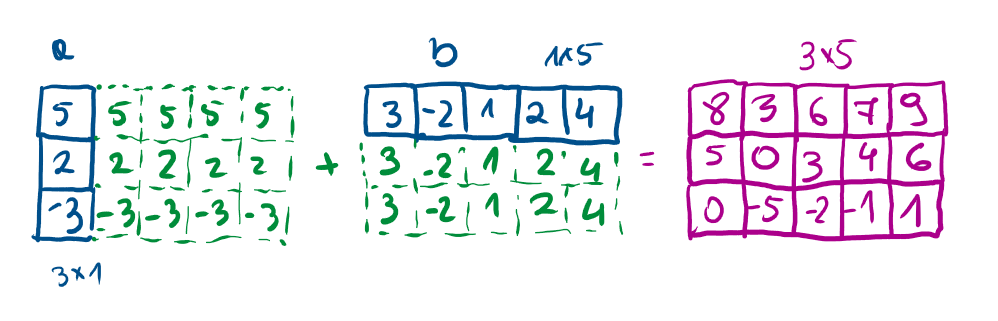
\includegraphics[keepaspectratio]{o5.png}}

\textbf{Ćwiczenia:} (\texttt{ex6.py})

\begin{enumerate}
\def\labelenumi{\arabic{enumi}.}
\item
  Rozważ jednowymiarową tablicę\\
  \[A = \begin{bmatrix}1 & 2 & 3\end{bmatrix}\]\\
  oraz skalar \(k = 10\).\\
  Wykonaj dodawanie, odejmowanie, mnożenie i dzielenie każdego elementu
  tablicy \(A\) przez \(k\) z wykorzystaniem broadcastingu.
\item
  Dla dwóch tablic jednowymiarowych\\
  \[B_1 = \begin{bmatrix}1 & 2 & 3\end{bmatrix}, \quad B_2 = \begin{bmatrix}4 & 5 & 6\end{bmatrix},\]\\
  wykonaj działanie \(B_1 + B_2\), \(B_1 - B_2\), \(B_1 * B_2\) oraz
  \(B_1 / B_2\) używając broadcastingu.
\item
  Mając dwie tablice dwuwymiarowe:\\
  \[C_1 = \begin{bmatrix}1 & 2 \\ 3 & 4\end{bmatrix}, \quad C_2 = \begin{bmatrix}10 & 20 \\ 30 & 40\end{bmatrix},\]\\
  dodaj je i odejmij od siebie, sprawdzając czy broadcasting zajdzie
  automatycznie.
\item
  Rozważ tablicę dwuwymiarową\\
  \[D = \begin{bmatrix}1 & 2 & 3 \\ 4 & 5 & 6\end{bmatrix}\]\\
  oraz wektor\\
  \[v = \begin{bmatrix}10 & 100 & 1000\end{bmatrix}.\]\\
  Wykonaj mnożenie i dzielenie elementowe tablicy \(D\) przez \(v\) z
  wykorzystaniem broadcastingu.
\item
  Dla tablicy\\
  \[E = \begin{bmatrix}2 & 4 & 6 \\ 8 & 10 & 12\end{bmatrix}\]\\
  podnieś każdy element do kwadratu, a następnie podziel przez wektor\\
  \[w = \begin{bmatrix}2 & 2 & 2\end{bmatrix}\]\\
  korzystając z broadcastingu.
\item
  Mając tablicę dwuwymiarową\\
  \[F = \begin{bmatrix}1 & 2 \\ 3 & 4 \\ 5 & 6\end{bmatrix},\]\\
  oraz skalar \(s = 2\), wykonaj \(F * s\), a następnie \(F^{s}\)
  (podnieś każdy element do potęgi \(s\)) z zastosowaniem broadcastingu.
\item
  Rozważ tablicę\\
  \[G = \begin{bmatrix}10 & 20 & 30\end{bmatrix}\]\\
  oraz kolumnową tablicę dwuwymiarową\\
  \[h = \begin{bmatrix}1 \\ 2 \\ 3\end{bmatrix}.\] Dodaj do \(h\)
  tablicę \(G\) i zaobserwuj wynik broadcastingu.
\item
  Mając dwie tablice dwuwymiarowe o różnych wymiarach:\\
  \[H_1 = \begin{bmatrix}1 & 2 & 3\end{bmatrix}, \quad H_2 = \begin{bmatrix}10 \\ 20 \\ 30\end{bmatrix},\]\\
  spróbuj je dodać i pomnożyć przez siebie, korzystając z broadcastingu.
\item
  Rozważ tablicę dwuwymiarową\\
  \[J = \begin{bmatrix}1 & 2 & 3 \\ 4 & 5 & 6\end{bmatrix}\]\\
  oraz skalar \(m = 5\).\\
  Wykonaj kombinację działań: najpierw pomnóż \(J\) przez \(m\),
  następnie odejmij \(m\), a na końcu podziel wynik przez \(m\) --
  wszystko z wykorzystaniem broadcastingu.
\end{enumerate}

\chapter{Funkcje uniwersalne (ufunc)}\label{funkcje-uniwersalne-ufunc}

Funkcje uniwersalne (tzw. \emph{ufunc}) to jedne z najważniejszych
narzędzi w NumPy. Są to funkcje działające element-po-elemencie na
tablicach, często implementowane w C, co zapewnia wysoką wydajność
obliczeń. Dzięki \emph{ufuncs} można w prosty i czytelny sposób
wykonywać operacje arytmetyczne, trygonometryczne, statystyczne czy
logiczne na całych tablicach bez konieczności pisania pętli w Pythonie.

\section{Podstawowe operacje
arytmetyczne}\label{podstawowe-operacje-arytmetyczne}

NumPy automatycznie przekształca operatory matematyczne w odpowiednie
\emph{ufunc}.\\
Na przykład:

\begin{itemize}
\tightlist
\item
  \texttt{+} odpowiada \texttt{np.add}
\item
  \texttt{-} odpowiada \texttt{np.subtract}
\item
  \texttt{*} odpowiada \texttt{np.multiply}
\item
  \texttt{/} odpowiada \texttt{np.divide}
\item
  \texttt{**} odpowiada \texttt{np.power}
\end{itemize}

Przykład:

\begin{Shaded}
\begin{Highlighting}[]
\ImportTok{import}\NormalTok{ numpy }\ImportTok{as}\NormalTok{ np}

\NormalTok{A }\OperatorTok{=}\NormalTok{ np.array([}\DecValTok{1}\NormalTok{, }\DecValTok{2}\NormalTok{, }\DecValTok{3}\NormalTok{, }\DecValTok{4}\NormalTok{])}
\NormalTok{B }\OperatorTok{=}\NormalTok{ np.array([}\DecValTok{10}\NormalTok{, }\DecValTok{20}\NormalTok{, }\DecValTok{30}\NormalTok{, }\DecValTok{40}\NormalTok{])}

\CommentTok{\# Operacje element{-}po{-}elemencie}
\NormalTok{sum\_tab }\OperatorTok{=}\NormalTok{ np.add(A, B)       }\CommentTok{\# to samo co A + B}
\NormalTok{diff\_tab }\OperatorTok{=}\NormalTok{ np.subtract(B, A) }\CommentTok{\# to samo co B {-} A}
\NormalTok{mul\_tab }\OperatorTok{=}\NormalTok{ np.multiply(A, }\DecValTok{2}\NormalTok{)  }\CommentTok{\# to samo co A * 2}
\NormalTok{pow\_tab }\OperatorTok{=}\NormalTok{ np.power(A, }\DecValTok{3}\NormalTok{)     }\CommentTok{\# to samo co A ** 3}

\BuiltInTok{print}\NormalTok{(}\StringTok{"Suma:"}\NormalTok{, sum\_tab)}
\BuiltInTok{print}\NormalTok{(}\StringTok{"Różnica:"}\NormalTok{, diff\_tab)}
\BuiltInTok{print}\NormalTok{(}\StringTok{"Mnożenie przez 2:"}\NormalTok{, mul\_tab)}
\BuiltInTok{print}\NormalTok{(}\StringTok{"Potęgowanie:"}\NormalTok{, pow\_tab)}
\end{Highlighting}
\end{Shaded}

\begin{verbatim}
Suma: [11 22 33 44]
Różnica: [ 9 18 27 36]
Mnożenie przez 2: [2 4 6 8]
Potęgowanie: [ 1  8 27 64]
\end{verbatim}

\section{Funkcje trygonometryczne i
pochodne}\label{funkcje-trygonometryczne-i-pochodne}

NumPy oferuje bogaty zestaw funkcji trygonometrycznych:

\begin{itemize}
\tightlist
\item
  \texttt{np.sin}, \texttt{np.cos}, \texttt{np.tan} -- funkcje
  podstawowe,
\item
  \texttt{np.arcsin}, \texttt{np.arccos}, \texttt{np.arctan} -- odwrotne
  funkcje trygonometryczne,
\item
  \texttt{np.sinh}, \texttt{np.cosh}, \texttt{np.tanh} -- funkcje
  hiperboliczne.
\end{itemize}

Przykład:

\begin{Shaded}
\begin{Highlighting}[]
\ImportTok{import}\NormalTok{ numpy }\ImportTok{as}\NormalTok{ np}

\NormalTok{x }\OperatorTok{=}\NormalTok{ np.linspace(}\DecValTok{0}\NormalTok{, np.pi, }\DecValTok{5}\NormalTok{) }\CommentTok{\# tablica [0, π/4, π/2, 3π/4, π]}
\NormalTok{sin\_values }\OperatorTok{=}\NormalTok{ np.sin(x)}
\NormalTok{cos\_values }\OperatorTok{=}\NormalTok{ np.cos(x)}

\BuiltInTok{print}\NormalTok{(}\StringTok{"Wartości sin(x):"}\NormalTok{, sin\_values)}
\BuiltInTok{print}\NormalTok{(}\StringTok{"Wartości cos(x):"}\NormalTok{, cos\_values)}
\end{Highlighting}
\end{Shaded}

\begin{verbatim}
Wartości sin(x): [0.00000000e+00 7.07106781e-01 1.00000000e+00 7.07106781e-01
 1.22464680e-16]
Wartości cos(x): [ 1.00000000e+00  7.07106781e-01  6.12323400e-17 -7.07106781e-01
 -1.00000000e+00]
\end{verbatim}

\section{Funkcje wykładnicze i
logarytmiczne}\label{funkcje-wykux142adnicze-i-logarytmiczne}

\begin{itemize}
\tightlist
\item
  \texttt{np.exp} -- eksponenta,
\item
  \texttt{np.log} -- logarytm naturalny,
\item
  \texttt{np.log10} -- logarytm dziesiętny.
\end{itemize}

Przykład:

\begin{Shaded}
\begin{Highlighting}[]
\ImportTok{import}\NormalTok{ numpy }\ImportTok{as}\NormalTok{ np}

\NormalTok{A }\OperatorTok{=}\NormalTok{ np.array([}\DecValTok{1}\NormalTok{, np.e, np.e}\OperatorTok{**}\DecValTok{2}\NormalTok{])}
\BuiltInTok{print}\NormalTok{(}\StringTok{"A:"}\NormalTok{, A)}
\BuiltInTok{print}\NormalTok{(}\StringTok{"log(A):"}\NormalTok{, np.log(A))}
\BuiltInTok{print}\NormalTok{(}\StringTok{"exp(A):"}\NormalTok{, np.exp([}\DecValTok{0}\NormalTok{, }\DecValTok{1}\NormalTok{, }\DecValTok{2}\NormalTok{]))  }\CommentTok{\# exp(0)=1, exp(1)=e, exp(2)=e\^{}2}
\end{Highlighting}
\end{Shaded}

\begin{verbatim}
A: [1.         2.71828183 7.3890561 ]
log(A): [0. 1. 2.]
exp(A): [1.         2.71828183 7.3890561 ]
\end{verbatim}

\section{Funkcje zaokrąglające i wartości
bezwzględne}\label{funkcje-zaokrux105glajux105ce-i-wartoux15bci-bezwzglux119dne}

\begin{itemize}
\tightlist
\item
  \texttt{np.round} -- zaokrągla do najbliższej liczby,
\item
  \texttt{np.floor} -- podłoga,
\item
  \texttt{np.ceil} -- sufit,
\item
  \texttt{np.trunc} -- obcięcie do części całkowitej,
\item
  \texttt{np.abs} -- wartość bezwzględna.
\end{itemize}

Przykład:

\begin{Shaded}
\begin{Highlighting}[]
\ImportTok{import}\NormalTok{ numpy }\ImportTok{as}\NormalTok{ np}

\NormalTok{B }\OperatorTok{=}\NormalTok{ np.array([}\FloatTok{1.7}\NormalTok{, }\OperatorTok{{-}}\FloatTok{2.5}\NormalTok{, }\FloatTok{3.5}\NormalTok{, }\OperatorTok{{-}}\FloatTok{4.1}\NormalTok{])}
\BuiltInTok{print}\NormalTok{(}\StringTok{"B:"}\NormalTok{, B)}
\BuiltInTok{print}\NormalTok{(}\StringTok{"floor(B):"}\NormalTok{, np.floor(B))}
\BuiltInTok{print}\NormalTok{(}\StringTok{"ceil(B):"}\NormalTok{, np.ceil(B))}
\BuiltInTok{print}\NormalTok{(}\StringTok{"abs(B):"}\NormalTok{, np.}\BuiltInTok{abs}\NormalTok{(B))}
\end{Highlighting}
\end{Shaded}

\begin{verbatim}
B: [ 1.7 -2.5  3.5 -4.1]
floor(B): [ 1. -3.  3. -5.]
ceil(B): [ 2. -2.  4. -4.]
abs(B): [1.7 2.5 3.5 4.1]
\end{verbatim}

\section{Funkcje statystyczne i
agregujące}\label{funkcje-statystyczne-i-agregujux105ce}

Choć wiele funkcji statystycznych dostępnych jest jako metody tablic
(np. \texttt{A.mean()}, \texttt{A.std()}), istnieją też ufuncs
działające element-po-elemencie lub akceptujące parametry osi:

\begin{itemize}
\tightlist
\item
  \texttt{np.minimum}, \texttt{np.maximum} -- zwracają minimum/maksimum
  element-po-elemencie z dwóch tablic,
\item
  \texttt{np.fmin}, \texttt{np.fmax} -- podobne do wyżej wymienionych,
  ale ignorują wartości NaN,
\item
  \texttt{np.sqrt} -- pierwiastek kwadratowy,
\item
  \texttt{np.square} -- podniesienie do kwadratu.
\end{itemize}

Przykład:

\begin{Shaded}
\begin{Highlighting}[]
\ImportTok{import}\NormalTok{ numpy }\ImportTok{as}\NormalTok{ np}

\NormalTok{C1 }\OperatorTok{=}\NormalTok{ np.array([}\DecValTok{1}\NormalTok{, }\DecValTok{4}\NormalTok{, }\DecValTok{9}\NormalTok{, }\DecValTok{16}\NormalTok{])}
\NormalTok{C2 }\OperatorTok{=}\NormalTok{ np.array([}\DecValTok{2}\NormalTok{, }\DecValTok{2}\NormalTok{, }\DecValTok{5}\NormalTok{, }\DecValTok{20}\NormalTok{])}

\BuiltInTok{print}\NormalTok{(}\StringTok{"minimum elementów C1 i C2:"}\NormalTok{, np.minimum(C1, C2))}
\BuiltInTok{print}\NormalTok{(}\StringTok{"maximum elementów C1 i C2:"}\NormalTok{, np.maximum(C1, C2))}
\BuiltInTok{print}\NormalTok{(}\StringTok{"sqrt(C1):"}\NormalTok{, np.sqrt(C1))}
\BuiltInTok{print}\NormalTok{(}\StringTok{"square(C2):"}\NormalTok{, np.square(C2))}
\end{Highlighting}
\end{Shaded}

\begin{verbatim}
minimum elementów C1 i C2: [ 1  2  5 16]
maximum elementów C1 i C2: [ 2  4  9 20]
sqrt(C1): [1. 2. 3. 4.]
square(C2): [  4   4  25 400]
\end{verbatim}

\textbf{Ćwiczenia:} (\texttt{ex7.py})

\begin{enumerate}
\def\labelenumi{\arabic{enumi}.}
\item
  Mając tablicę\\
  \[A = \begin{bmatrix}1 & 4 & 9 & 16\end{bmatrix},\]\\
  zastosuj funkcję uniwersalną, aby obliczyć pierwiastek kwadratowy
  każdego elementu.
\item
  Rozważ jednowymiarową tablicę\\
  \[B = \begin{bmatrix}-1 & -2 & 3 & -4\end{bmatrix},\]\\
  zastosuj funkcję uniwersalną, aby otrzymać wartości bezwzględne
  wszystkich elementów.
\item
  Dla tablicy\\
  \[C = \begin{bmatrix}0 & \pi/2 & \pi & 3\pi/2\end{bmatrix},\]\\
  oblicz wartość funkcji trygonometrycznej dla każdego elementu.
\item
  Mając tablicę\\
  \[D = \begin{bmatrix}1 & e & e^2 \end{bmatrix},\]\\
  zastosuj funkcję uniwersalną, aby obliczyć logarytm naturalny każdego
  elementu.
\item
  Dla tablicy dwuwymiarowej\\
  \[E = \begin{bmatrix}2 & 4 \\ 10 & 20 \end{bmatrix},\]\\
  podziel każdy element przez skalar, a następnie podnieś uzyskane
  wartości do kwadratu.
\item
  Rozważ tablicę\\
  \[F = \begin{bmatrix}1 & 2 & 3\end{bmatrix},\]\\
  podnieś każdy element do trzeciej potęgi, a następnie zastosuj funkcję
  uniwersalną, aby obliczyć eksponentę z otrzymanych wartości.
\item
  Mając tablicę\\
  \[G = \begin{bmatrix}-\pi & -\pi/2 & 0 & \pi/2 & \pi\end{bmatrix},\]\\
  zastosuj odpowiednią funkcję uniwersalną, aby uzyskać cosinus każdego
  elementu.
\item
  Dla tablicy\\
  \[H = \begin{bmatrix}10 & 100 & 1000\end{bmatrix},\]\\
  zastosuj funkcję uniwersalną, aby obliczyć logarytm dziesiętny każdego
  elementu.
\item
  Mając tablicę\\
  \[I = \begin{bmatrix}2 & 8 & 18 & 32\end{bmatrix},\]\\
  przekształć ją, stosując funkcję uniwersalną, tak aby każdy element
  był pierwiastkiem kwadratowym z wartości początkowej, a następnie
  pomnóż wyniki przez 2.
\item
  Rozważ tablicę\\
  \[J = \begin{bmatrix}-1 & -4 & -9 & -16\end{bmatrix},\]\\
  oblicz pierwiastek kwadratowy wartości bezwzględnych elementów tej
  tablicy, wykorzystując po kolei dwie różne funkcje uniwersalne.
\end{enumerate}

\chapter{Operacje na stringach}\label{operacje-na-stringach}

W \texttt{NumPy} poza dobrze znanymi tablicami liczbowymi, istnieje
również zestaw funkcji pozwalających na wektorowe operacje na ciągach
znaków.

\textbf{Ważne:} Poniższe funkcje są zazwyczaj dostępne w module
\texttt{numpy.char}. W dokumentacji znajdują się one w sekcji
\href{https://numpy.org/doc/stable/reference/routines.strings.html}{String
operations}, jednak w tym materiale skupimy się na tym, jak można je
wykorzystywać, zakładając interfejs z modułu \texttt{numpy.strings}.
Jest to analogiczne do korzystania z \texttt{numpy.char}. Jest no nowsze
podejście.

\section{Tworzenie tablic z napisami}\label{tworzenie-tablic-z-napisami}

NumPy pozwala na przechowywanie tekstu w tablicach, np. tak:

\begin{Shaded}
\begin{Highlighting}[]
\ImportTok{import}\NormalTok{ numpy }\ImportTok{as}\NormalTok{ np}

\NormalTok{arr }\OperatorTok{=}\NormalTok{ np.array([}\StringTok{"python"}\NormalTok{, }\StringTok{"NumPy"}\NormalTok{, }\StringTok{"data"}\NormalTok{, }\StringTok{"Science"}\NormalTok{])}
\BuiltInTok{print}\NormalTok{(arr)}
\end{Highlighting}
\end{Shaded}

\begin{verbatim}
['python' 'NumPy' 'data' 'Science']
\end{verbatim}

\begin{center}\rule{0.5\linewidth}{0.5pt}\end{center}

\section{Podstawowe funkcje do modyfikacji
tekstu}\label{podstawowe-funkcje-do-modyfikacji-tekstu}

Poniżej przedstawiono popularne funkcje do modyfikacji tekstu na
tablicach stringów:

\subsection{\texorpdfstring{\texttt{numpy.strings.upper} i
\texttt{numpy.strings.lower}}{numpy.strings.upper i numpy.strings.lower}}\label{numpy.strings.upper-i-numpy.strings.lower}

\begin{itemize}
\tightlist
\item
  \texttt{upper}: Zamiana wszystkich liter na wielkie.
\item
  \texttt{lower}: Zamiana wszystkich liter na małe.
\end{itemize}

\begin{Shaded}
\begin{Highlighting}[]
\ImportTok{import}\NormalTok{ numpy }\ImportTok{as}\NormalTok{ np}

\NormalTok{arr }\OperatorTok{=}\NormalTok{ np.array([}\StringTok{"python"}\NormalTok{, }\StringTok{"NumPy"}\NormalTok{, }\StringTok{"data"}\NormalTok{, }\StringTok{"Science"}\NormalTok{])}

\BuiltInTok{print}\NormalTok{(np.strings.upper(arr))}
\BuiltInTok{print}\NormalTok{(np.strings.lower(arr))}
\end{Highlighting}
\end{Shaded}

\begin{verbatim}
['PYTHON' 'NUMPY' 'DATA' 'SCIENCE']
['python' 'numpy' 'data' 'science']
\end{verbatim}

\subsection{\texorpdfstring{\texttt{numpy.strings.capitalize}}{numpy.strings.capitalize}}\label{numpy.strings.capitalize}

Funkcja \texttt{capitalize} zamienia pierwszą literę wyrazu na wielką, a
pozostałe na małe.

\begin{Shaded}
\begin{Highlighting}[]
\ImportTok{import}\NormalTok{ numpy }\ImportTok{as}\NormalTok{ np}

\NormalTok{arr }\OperatorTok{=}\NormalTok{ np.array([}\StringTok{"python"}\NormalTok{, }\StringTok{"NumPy"}\NormalTok{, }\StringTok{"data"}\NormalTok{, }\StringTok{"Science"}\NormalTok{])}
\BuiltInTok{print}\NormalTok{(np.strings.capitalize(arr))}
\end{Highlighting}
\end{Shaded}

\begin{verbatim}
['Python' 'Numpy' 'Data' 'Science']
\end{verbatim}

\subsection{\texorpdfstring{\texttt{numpy.strings.title}}{numpy.strings.title}}\label{numpy.strings.title}

Funkcja \texttt{title} sprawia, że każda część składowa tekstu (np.
oddzielona spacją) zostaje zamieniona tak, by zaczynała się od wielkiej
litery.

\begin{Shaded}
\begin{Highlighting}[]
\ImportTok{import}\NormalTok{ numpy }\ImportTok{as}\NormalTok{ np}

\NormalTok{arr2 }\OperatorTok{=}\NormalTok{ np.array([}\StringTok{"python data science"}\NormalTok{, }\StringTok{"machine learning"}\NormalTok{, }\StringTok{"deep learning"}\NormalTok{])}
\BuiltInTok{print}\NormalTok{(np.strings.title(arr2))}
\end{Highlighting}
\end{Shaded}

\begin{verbatim}
['Python Data Science' 'Machine Learning' 'Deep Learning']
\end{verbatim}

\begin{center}\rule{0.5\linewidth}{0.5pt}\end{center}

\section{Łączenie i rozdzielanie
tekstów}\label{ux142ux105czenie-i-rozdzielanie-tekstuxf3w}

\subsection{\texorpdfstring{\texttt{numpy.strings.add}}{numpy.strings.add}}\label{numpy.strings.add}

Funkcja \texttt{add} łączy elementy tablic tekstowych, działając
podobnie jak operator \texttt{+} na stringach, ale wektorowo.

\begin{Shaded}
\begin{Highlighting}[]
\ImportTok{import}\NormalTok{ numpy }\ImportTok{as}\NormalTok{ np}

\NormalTok{arr\_a }\OperatorTok{=}\NormalTok{ np.array([}\StringTok{"Hello"}\NormalTok{, }\StringTok{"Data"}\NormalTok{])}
\NormalTok{arr\_b }\OperatorTok{=}\NormalTok{ np.array([}\StringTok{"World"}\NormalTok{, }\StringTok{"Science"}\NormalTok{])}

\BuiltInTok{print}\NormalTok{(np.strings.add(arr\_a, arr\_b))}
\end{Highlighting}
\end{Shaded}

\begin{verbatim}
['HelloWorld' 'DataScience']
\end{verbatim}

\subsection{\texorpdfstring{\texttt{numpy.strings.join}}{numpy.strings.join}}\label{numpy.strings.join}

Funkcja \texttt{join} pozwala na łączenie elementów tablicy przy użyciu
wskazanego separatora.

\begin{Shaded}
\begin{Highlighting}[]
\ImportTok{import}\NormalTok{ numpy }\ImportTok{as}\NormalTok{ np}

\NormalTok{arr3 }\OperatorTok{=}\NormalTok{ np.array([}\StringTok{"python"}\NormalTok{, }\StringTok{"numpy"}\NormalTok{, }\StringTok{"string"}\NormalTok{])}
\BuiltInTok{print}\NormalTok{(np.char.join(}\StringTok{"{-}"}\NormalTok{, arr3))}
\end{Highlighting}
\end{Shaded}

\begin{verbatim}
['p-y-t-h-o-n' 'n-u-m-p-y' 's-t-r-i-n-g']
\end{verbatim}

\begin{quote}
Uwaga: \texttt{join} wektoryzuje operację, traktując każdy element
tablicy jako sekwencję znaków do połączenia separatorem.
\end{quote}

\subsection{\texorpdfstring{\texttt{numpy.strings.split}}{numpy.strings.split}}\label{numpy.strings.split}

Pozwala na rozdzielanie stringów według podanego separatora. Zwraca
tablicę zawierającą listy podłańcuchów.

\begin{Shaded}
\begin{Highlighting}[]
\ImportTok{import}\NormalTok{ numpy }\ImportTok{as}\NormalTok{ np}

\NormalTok{arr4 }\OperatorTok{=}\NormalTok{ np.array([}\StringTok{"python{-}data{-}science"}\NormalTok{, }\StringTok{"machine{-}learning"}\NormalTok{])}
\BuiltInTok{print}\NormalTok{(np.char.split(arr4, sep}\OperatorTok{=}\StringTok{"{-}"}\NormalTok{))}
\end{Highlighting}
\end{Shaded}

\begin{verbatim}
[list(['python', 'data', 'science']) list(['machine', 'learning'])]
\end{verbatim}

\begin{center}\rule{0.5\linewidth}{0.5pt}\end{center}

\section{Wyszukiwanie i zamiana
podciągów}\label{wyszukiwanie-i-zamiana-podciux105guxf3w}

\subsection{\texorpdfstring{\texttt{numpy.strings.find} i
\texttt{numpy.strings.rfind}}{numpy.strings.find i numpy.strings.rfind}}\label{numpy.strings.find-i-numpy.strings.rfind}

\begin{itemize}
\tightlist
\item
  \texttt{find}: Zwraca indeks pierwszego wystąpienia podłańcucha (lub
  -1, jeśli nie znaleziono).
\item
  \texttt{rfind}: Zwraca indeks ostatniego wystąpienia podłańcucha (lub
  -1, jeśli nie znaleziono).
\end{itemize}

\begin{Shaded}
\begin{Highlighting}[]
\ImportTok{import}\NormalTok{ numpy }\ImportTok{as}\NormalTok{ np}

\NormalTok{arr5 }\OperatorTok{=}\NormalTok{ np.array([}\StringTok{"python"}\NormalTok{, }\StringTok{"data"}\NormalTok{, }\StringTok{"numpy"}\NormalTok{])}
\BuiltInTok{print}\NormalTok{(np.strings.find(arr5, }\StringTok{"a"}\NormalTok{))}
\end{Highlighting}
\end{Shaded}

\begin{verbatim}
[-1  1 -1]
\end{verbatim}

\subsection{\texorpdfstring{\texttt{numpy.strings.replace}}{numpy.strings.replace}}\label{numpy.strings.replace}

\texttt{replace} zamienia wszystkie wystąpienia podłańcucha na nowy ciąg
znaków.

\begin{Shaded}
\begin{Highlighting}[]
\ImportTok{import}\NormalTok{ numpy }\ImportTok{as}\NormalTok{ np}

\NormalTok{arr6 }\OperatorTok{=}\NormalTok{ np.array([}\StringTok{"python"}\NormalTok{, }\StringTok{"pydata"}\NormalTok{, }\StringTok{"pypy"}\NormalTok{])}
\BuiltInTok{print}\NormalTok{(np.strings.replace(arr6, }\StringTok{"py"}\NormalTok{, }\StringTok{"PY"}\NormalTok{))}
\end{Highlighting}
\end{Shaded}

\begin{verbatim}
['PYthon' 'PYdata' 'PYPY']
\end{verbatim}

\begin{center}\rule{0.5\linewidth}{0.5pt}\end{center}

\section{Usuwanie zbędnych
znaków}\label{usuwanie-zbux119dnych-znakuxf3w}

\subsection{\texorpdfstring{\texttt{numpy.strings.strip},
\texttt{numpy.strings.lstrip} i
\texttt{numpy.strings.rstrip}}{numpy.strings.strip, numpy.strings.lstrip i numpy.strings.rstrip}}\label{numpy.strings.strip-numpy.strings.lstrip-i-numpy.strings.rstrip}

\begin{itemize}
\tightlist
\item
  \texttt{strip}: Usuwa wskazane znaki z początku i końca.
\item
  \texttt{lstrip}: Usuwa wskazane znaki z lewej strony (początku).
\item
  \texttt{rstrip}: Usuwa wskazane znaki z prawej strony (końca).
\end{itemize}

\begin{Shaded}
\begin{Highlighting}[]
\ImportTok{import}\NormalTok{ numpy }\ImportTok{as}\NormalTok{ np}

\NormalTok{arr7 }\OperatorTok{=}\NormalTok{ np.array([}\StringTok{"   python   "}\NormalTok{, }\StringTok{"  numpy  "}\NormalTok{])}
\BuiltInTok{print}\NormalTok{(np.strings.strip(arr7))}
\end{Highlighting}
\end{Shaded}

\begin{verbatim}
['python' 'numpy']
\end{verbatim}

Możemy również podać niestandardowe znaki do usunięcia:

\begin{Shaded}
\begin{Highlighting}[]
\ImportTok{import}\NormalTok{ numpy }\ImportTok{as}\NormalTok{ np}

\NormalTok{arr8 }\OperatorTok{=}\NormalTok{ np.array([}\StringTok{"\#\#\#data\#\#\#"}\NormalTok{, }\StringTok{"***science***"}\NormalTok{])}
\BuiltInTok{print}\NormalTok{(np.strings.strip(arr8, }\StringTok{"\#*"}\NormalTok{))}
\end{Highlighting}
\end{Shaded}

\begin{verbatim}
['data' 'science']
\end{verbatim}

\chapter{Alegbra liniowa}\label{alegbra-liniowa}

\section{Iloczyn skalarny (dot
product)}\label{iloczyn-skalarny-dot-product}

Dla dwóch wektorów, \texttt{dot} oblicza ich iloczyn skalarny.

\begin{Shaded}
\begin{Highlighting}[]
\ImportTok{import}\NormalTok{ numpy }\ImportTok{as}\NormalTok{ np}

\CommentTok{\# Iloczyn skalarny dwóch wektorów}
\NormalTok{a }\OperatorTok{=}\NormalTok{ np.array([}\DecValTok{1}\NormalTok{, }\DecValTok{2}\NormalTok{, }\DecValTok{3}\NormalTok{])}
\NormalTok{b }\OperatorTok{=}\NormalTok{ np.array([}\DecValTok{4}\NormalTok{, }\DecValTok{5}\NormalTok{, }\DecValTok{6}\NormalTok{])}
\NormalTok{result }\OperatorTok{=}\NormalTok{ np.dot(a, b)  }\CommentTok{\# 1*4 + 2*5 + 3*6}
\BuiltInTok{print}\NormalTok{(result)  }\CommentTok{\# Wynik: 32}

\CommentTok{\# Alternatywny zapis za pomocą operatora @}
\NormalTok{result }\OperatorTok{=}\NormalTok{ a }\OperatorTok{@}\NormalTok{ b}
\BuiltInTok{print}\NormalTok{(result)  }\CommentTok{\# Wynik: 32}
\end{Highlighting}
\end{Shaded}

\begin{verbatim}
32
32
\end{verbatim}

\section{Mnożenie macierzowe}\label{mnoux17cenie-macierzowe}

Dla macierzy (tablic dwuwymiarowych), \texttt{dot} wykonuje standardowe
mnożenie macierzowe.

\begin{Shaded}
\begin{Highlighting}[]
\ImportTok{import}\NormalTok{ numpy }\ImportTok{as}\NormalTok{ np}
\CommentTok{\# Mnożenie macierzowe}
\NormalTok{A }\OperatorTok{=}\NormalTok{ np.array([[}\DecValTok{1}\NormalTok{, }\DecValTok{2}\NormalTok{], [}\DecValTok{3}\NormalTok{, }\DecValTok{4}\NormalTok{]])}
\NormalTok{B }\OperatorTok{=}\NormalTok{ np.array([[}\DecValTok{5}\NormalTok{, }\DecValTok{6}\NormalTok{], [}\DecValTok{7}\NormalTok{, }\DecValTok{8}\NormalTok{]])}
\NormalTok{C }\OperatorTok{=}\NormalTok{ np.dot(A, B)}
\BuiltInTok{print}\NormalTok{(C)}
\CommentTok{\# Wynik:}
\CommentTok{\# [[19 22]}
\CommentTok{\#  [43 50]]}

\CommentTok{\# To samo za pomocą operatora @}
\NormalTok{C }\OperatorTok{=}\NormalTok{ A }\OperatorTok{@}\NormalTok{ B}
\BuiltInTok{print}\NormalTok{(C)}
\end{Highlighting}
\end{Shaded}

\begin{verbatim}
[[19 22]
 [43 50]]
[[19 22]
 [43 50]]
\end{verbatim}

\section{Mnożenie macierz-wektor}\label{mnoux17cenie-macierz-wektor}

Możemy również mnożyć macierz przez wektor:

\begin{Shaded}
\begin{Highlighting}[]
\ImportTok{import}\NormalTok{ numpy }\ImportTok{as}\NormalTok{ np}
\CommentTok{\# Mnożenie macierz{-}wektor}
\NormalTok{A }\OperatorTok{=}\NormalTok{ np.array([[}\DecValTok{1}\NormalTok{, }\DecValTok{2}\NormalTok{], [}\DecValTok{3}\NormalTok{, }\DecValTok{4}\NormalTok{]])}
\NormalTok{v }\OperatorTok{=}\NormalTok{ np.array([}\DecValTok{5}\NormalTok{, }\DecValTok{6}\NormalTok{])}
\NormalTok{result }\OperatorTok{=}\NormalTok{ np.dot(A, v)}
\BuiltInTok{print}\NormalTok{(result)  }\CommentTok{\# Wynik: [17 39]}
\end{Highlighting}
\end{Shaded}

\begin{verbatim}
[17 39]
\end{verbatim}

\section{Rozwiązywanie układów równań
liniowych}\label{rozwiux105zywanie-ukux142aduxf3w-ruxf3wnaux144-liniowych}

Funkcja \texttt{numpy.linalg.solve} rozwiązuje układy równań liniowych
postaci Ax = b:

\begin{Shaded}
\begin{Highlighting}[]
\ImportTok{import}\NormalTok{ numpy }\ImportTok{as}\NormalTok{ np}
\CommentTok{\# Rozwiązywanie układu równań liniowych}
\NormalTok{A }\OperatorTok{=}\NormalTok{ np.array([[}\DecValTok{3}\NormalTok{, }\DecValTok{1}\NormalTok{], [}\DecValTok{1}\NormalTok{, }\DecValTok{2}\NormalTok{]])}
\NormalTok{b }\OperatorTok{=}\NormalTok{ np.array([}\DecValTok{9}\NormalTok{, }\DecValTok{8}\NormalTok{])}
\NormalTok{x }\OperatorTok{=}\NormalTok{ np.linalg.solve(A, b)}
\BuiltInTok{print}\NormalTok{(x)  }\CommentTok{\# Wynik: [2. 3.]}

\CommentTok{\# Sprawdzenie rozwiązania}
\NormalTok{np.dot(A, x)  }\CommentTok{\# Powinno być równe b}
\end{Highlighting}
\end{Shaded}

\begin{verbatim}
[2. 3.]
\end{verbatim}

\begin{verbatim}
array([9., 8.])
\end{verbatim}

\section{Wyznacznik macierzy}\label{wyznacznik-macierzy}

Funkcja \texttt{numpy.linalg.det} oblicza wyznacznik macierzy:

\begin{Shaded}
\begin{Highlighting}[]
\ImportTok{import}\NormalTok{ numpy }\ImportTok{as}\NormalTok{ np}
\CommentTok{\# Obliczanie wyznacznika}
\NormalTok{A }\OperatorTok{=}\NormalTok{ np.array([[}\DecValTok{1}\NormalTok{, }\DecValTok{2}\NormalTok{], [}\DecValTok{3}\NormalTok{, }\DecValTok{4}\NormalTok{]])}
\NormalTok{det\_A }\OperatorTok{=}\NormalTok{ np.linalg.det(A)}
\BuiltInTok{print}\NormalTok{(det\_A)  }\CommentTok{\# Wynik: {-}2.0}
\end{Highlighting}
\end{Shaded}

\begin{verbatim}
-2.0000000000000004
\end{verbatim}

\section{Wartości i wektory
własne}\label{wartoux15bci-i-wektory-wux142asne}

Funkcja \texttt{numpy.linalg.eig} oblicza wartości i wektory własne
macierzy:

\begin{Shaded}
\begin{Highlighting}[]
\ImportTok{import}\NormalTok{ numpy }\ImportTok{as}\NormalTok{ np}
\CommentTok{\# Obliczanie wartości i wektorów własnych}
\NormalTok{A }\OperatorTok{=}\NormalTok{ np.array([[}\DecValTok{4}\NormalTok{, }\OperatorTok{{-}}\DecValTok{2}\NormalTok{], [}\DecValTok{1}\NormalTok{, }\DecValTok{1}\NormalTok{]])}
\NormalTok{eigenvalues, eigenvectors }\OperatorTok{=}\NormalTok{ np.linalg.eig(A)}
\BuiltInTok{print}\NormalTok{(}\StringTok{"Wartości własne:"}\NormalTok{, eigenvalues)}
\BuiltInTok{print}\NormalTok{(}\StringTok{"Wektory własne:"}\NormalTok{)}
\BuiltInTok{print}\NormalTok{(eigenvectors)}

\CommentTok{\# Sprawdzenie: A * v = lambda * v}
\ControlFlowTok{for}\NormalTok{ i }\KeywordTok{in} \BuiltInTok{range}\NormalTok{(}\BuiltInTok{len}\NormalTok{(eigenvalues)):}
\NormalTok{    lambda\_i }\OperatorTok{=}\NormalTok{ eigenvalues[i]}
\NormalTok{    v\_i }\OperatorTok{=}\NormalTok{ eigenvectors[:, i]}
    \BuiltInTok{print}\NormalTok{(}\SpecialStringTok{f"λ\_}\SpecialCharTok{\{}\NormalTok{i}\SpecialCharTok{\}}\SpecialStringTok{ = }\SpecialCharTok{\{}\NormalTok{lambda\_i}\SpecialCharTok{\}}\SpecialStringTok{"}\NormalTok{)}
    \BuiltInTok{print}\NormalTok{(}\StringTok{"A * v ="}\NormalTok{, np.dot(A, v\_i))}
    \BuiltInTok{print}\NormalTok{(}\StringTok{"λ * v ="}\NormalTok{, lambda\_i }\OperatorTok{*}\NormalTok{ v\_i)}
\end{Highlighting}
\end{Shaded}

\begin{verbatim}
Wartości własne: [3. 2.]
Wektory własne:
[[0.89442719 0.70710678]
 [0.4472136  0.70710678]]
λ_0 = 3.0
A * v = [2.68328157 1.34164079]
λ * v = [2.68328157 1.34164079]
λ_1 = 2.0
A * v = [1.41421356 1.41421356]
λ * v = [1.41421356 1.41421356]
\end{verbatim}

\section{Rozkład wartości osobliwych
(SVD)}\label{rozkux142ad-wartoux15bci-osobliwych-svd}

Rozkład SVD jest potężnym narzędziem w analizie danych:

\begin{Shaded}
\begin{Highlighting}[]
\ImportTok{import}\NormalTok{ numpy }\ImportTok{as}\NormalTok{ np}
\CommentTok{\# Rozkład SVD}
\NormalTok{A }\OperatorTok{=}\NormalTok{ np.array([[}\DecValTok{1}\NormalTok{, }\DecValTok{2}\NormalTok{], [}\DecValTok{3}\NormalTok{, }\DecValTok{4}\NormalTok{], [}\DecValTok{5}\NormalTok{, }\DecValTok{6}\NormalTok{]])}
\NormalTok{U, s, Vh }\OperatorTok{=}\NormalTok{ np.linalg.svd(A)}
\BuiltInTok{print}\NormalTok{(}\StringTok{"Macierz U:"}\NormalTok{)}
\BuiltInTok{print}\NormalTok{(U)}
\BuiltInTok{print}\NormalTok{(}\StringTok{"Wartości osobliwe:"}\NormalTok{, s)}
\BuiltInTok{print}\NormalTok{(}\StringTok{"Macierz V\^{}H:"}\NormalTok{)}
\BuiltInTok{print}\NormalTok{(Vh)}

\CommentTok{\# Rekonstrukcja macierzy A}
\NormalTok{S }\OperatorTok{=}\NormalTok{ np.zeros((A.shape[}\DecValTok{0}\NormalTok{], A.shape[}\DecValTok{1}\NormalTok{]))}
\NormalTok{S[:}\BuiltInTok{len}\NormalTok{(s), :}\BuiltInTok{len}\NormalTok{(s)] }\OperatorTok{=}\NormalTok{ np.diag(s)}
\NormalTok{A\_reconstructed }\OperatorTok{=}\NormalTok{ U }\OperatorTok{@}\NormalTok{ S }\OperatorTok{@}\NormalTok{ Vh}
\BuiltInTok{print}\NormalTok{(}\StringTok{"Rekonstruowana macierz A:"}\NormalTok{)}
\BuiltInTok{print}\NormalTok{(A\_reconstructed)}
\end{Highlighting}
\end{Shaded}

\begin{verbatim}
Macierz U:
[[-0.2298477   0.88346102  0.40824829]
 [-0.52474482  0.24078249 -0.81649658]
 [-0.81964194 -0.40189603  0.40824829]]
Wartości osobliwe: [9.52551809 0.51430058]
Macierz V^H:
[[-0.61962948 -0.78489445]
 [-0.78489445  0.61962948]]
Rekonstruowana macierz A:
[[1. 2.]
 [3. 4.]
 [5. 6.]]
\end{verbatim}

\section{Norma macierzy/wektora}\label{norma-macierzywektora}

NumPy oferuje różne rodzaje norm:

\begin{Shaded}
\begin{Highlighting}[]
\ImportTok{import}\NormalTok{ numpy }\ImportTok{as}\NormalTok{ np}
\CommentTok{\# Różne normy}
\NormalTok{v }\OperatorTok{=}\NormalTok{ np.array([}\DecValTok{3}\NormalTok{, }\DecValTok{4}\NormalTok{])}
\BuiltInTok{print}\NormalTok{(}\StringTok{"Norma L1:"}\NormalTok{, np.linalg.norm(v, }\DecValTok{1}\NormalTok{))  }\CommentTok{\# Norma L1: 7.0}
\BuiltInTok{print}\NormalTok{(}\StringTok{"Norma L2 (Euklidesowa):"}\NormalTok{, np.linalg.norm(v))  }\CommentTok{\# Norma L2: 5.0}
\BuiltInTok{print}\NormalTok{(}\StringTok{"Norma maksimum:"}\NormalTok{, np.linalg.norm(v, np.inf))  }\CommentTok{\# Norma maksimum: 4.0}

\NormalTok{A }\OperatorTok{=}\NormalTok{ np.array([[}\DecValTok{1}\NormalTok{, }\DecValTok{2}\NormalTok{], [}\DecValTok{3}\NormalTok{, }\DecValTok{4}\NormalTok{]])}
\BuiltInTok{print}\NormalTok{(}\StringTok{"Norma macierzowa Frobeniusa:"}\NormalTok{, np.linalg.norm(A, }\StringTok{\textquotesingle{}fro\textquotesingle{}}\NormalTok{))  }\CommentTok{\# Norma Frobeniusa: 5.477...}
\end{Highlighting}
\end{Shaded}

\begin{verbatim}
Norma L1: 7.0
Norma L2 (Euklidesowa): 5.0
Norma maksimum: 4.0
Norma macierzowa Frobeniusa: 5.477225575051661
\end{verbatim}

\section{Macierz odwrotna}\label{macierz-odwrotna}

Funkcja \texttt{numpy.linalg.inv} oblicza macierz odwrotną:

\begin{Shaded}
\begin{Highlighting}[]
\ImportTok{import}\NormalTok{ numpy }\ImportTok{as}\NormalTok{ np}
\CommentTok{\# Macierz odwrotna}
\NormalTok{A }\OperatorTok{=}\NormalTok{ np.array([[}\DecValTok{1}\NormalTok{, }\DecValTok{2}\NormalTok{], [}\DecValTok{3}\NormalTok{, }\DecValTok{4}\NormalTok{]])}
\NormalTok{A\_inv }\OperatorTok{=}\NormalTok{ np.linalg.inv(A)}
\BuiltInTok{print}\NormalTok{(}\StringTok{"Macierz odwrotna:"}\NormalTok{)}
\BuiltInTok{print}\NormalTok{(A\_inv)}

\CommentTok{\# Sprawdzenie: A * A\^{}({-}1) = I}
\BuiltInTok{print}\NormalTok{(}\StringTok{"A * A\^{}({-}1):"}\NormalTok{)}
\BuiltInTok{print}\NormalTok{(np.dot(A, A\_inv))  }\CommentTok{\# Powinno być bliskie macierzy jednostkowej}
\end{Highlighting}
\end{Shaded}

\begin{verbatim}
Macierz odwrotna:
[[-2.   1. ]
 [ 1.5 -0.5]]
A * A^(-1):
[[1.0000000e+00 0.0000000e+00]
 [8.8817842e-16 1.0000000e+00]]
\end{verbatim}

\section{\texorpdfstring{Funkcja \texttt{numpy.inner} - iloczyn
wewnętrzny}{Funkcja numpy.inner - iloczyn wewnętrzny}}\label{funkcja-numpy.inner---iloczyn-wewnux119trzny}

Funkcja \texttt{inner} oblicza iloczyn wewnętrzny dwóch tablic:

\begin{Shaded}
\begin{Highlighting}[]
\ImportTok{import}\NormalTok{ numpy }\ImportTok{as}\NormalTok{ np}
\CommentTok{\# Iloczyn wewnętrzny}
\NormalTok{a }\OperatorTok{=}\NormalTok{ np.array([}\DecValTok{1}\NormalTok{, }\DecValTok{2}\NormalTok{, }\DecValTok{3}\NormalTok{])}
\NormalTok{b }\OperatorTok{=}\NormalTok{ np.array([}\DecValTok{4}\NormalTok{, }\DecValTok{5}\NormalTok{, }\DecValTok{6}\NormalTok{])}
\NormalTok{result }\OperatorTok{=}\NormalTok{ np.inner(a, b)}
\BuiltInTok{print}\NormalTok{(result)  }\CommentTok{\# 1*4 + 2*5 + 3*6 = 32}

\CommentTok{\# Dla tablic 2D}
\NormalTok{A }\OperatorTok{=}\NormalTok{ np.array([[}\DecValTok{1}\NormalTok{, }\DecValTok{2}\NormalTok{], [}\DecValTok{3}\NormalTok{, }\DecValTok{4}\NormalTok{]])}
\NormalTok{B }\OperatorTok{=}\NormalTok{ np.array([[}\DecValTok{5}\NormalTok{, }\DecValTok{6}\NormalTok{], [}\DecValTok{7}\NormalTok{, }\DecValTok{8}\NormalTok{]])}
\NormalTok{result }\OperatorTok{=}\NormalTok{ np.inner(A, B)}
\BuiltInTok{print}\NormalTok{(result)}
\CommentTok{\# Jest to równoważne wykonaniu iloczynu skalarnego wzdłuż ostatniego wymiaru}
\end{Highlighting}
\end{Shaded}

\begin{verbatim}
32
[[17 23]
 [39 53]]
\end{verbatim}

\section{\texorpdfstring{Funkcja \texttt{numpy.outer} - iloczyn
zewnętrzny}{Funkcja numpy.outer - iloczyn zewnętrzny}}\label{funkcja-numpy.outer---iloczyn-zewnux119trzny}

Funkcja \texttt{outer} oblicza iloczyn zewnętrzny dwóch wektorów:

\begin{Shaded}
\begin{Highlighting}[]
\ImportTok{import}\NormalTok{ numpy }\ImportTok{as}\NormalTok{ np}
\CommentTok{\# Iloczyn zewnętrzny}
\NormalTok{a }\OperatorTok{=}\NormalTok{ np.array([}\DecValTok{1}\NormalTok{, }\DecValTok{2}\NormalTok{, }\DecValTok{3}\NormalTok{])}
\NormalTok{b }\OperatorTok{=}\NormalTok{ np.array([}\DecValTok{4}\NormalTok{, }\DecValTok{5}\NormalTok{, }\DecValTok{6}\NormalTok{])}
\NormalTok{result }\OperatorTok{=}\NormalTok{ np.outer(a, b)}
\BuiltInTok{print}\NormalTok{(result)}
\CommentTok{\# Wynik:}
\CommentTok{\# [[ 4  5  6]}
\CommentTok{\#  [ 8 10 12]}
\CommentTok{\#  [12 15 18]]}
\end{Highlighting}
\end{Shaded}

\begin{verbatim}
[[ 4  5  6]
 [ 8 10 12]
 [12 15 18]]
\end{verbatim}

\section{\texorpdfstring{Funkcja \texttt{numpy.matmul} - mnożenie
macierzowe}{Funkcja numpy.matmul - mnożenie macierzowe}}\label{funkcja-numpy.matmul---mnoux17cenie-macierzowe}

Funkcja \texttt{matmul} jest podobna do \texttt{dot}, ale ma nieco inne
zachowanie dla tablic o wymiarach większych niż 2:

\begin{Shaded}
\begin{Highlighting}[]
\ImportTok{import}\NormalTok{ numpy }\ImportTok{as}\NormalTok{ np}
\CommentTok{\# Porównanie dot i matmul}
\NormalTok{a }\OperatorTok{=}\NormalTok{ np.array([[}\DecValTok{1}\NormalTok{, }\DecValTok{2}\NormalTok{], [}\DecValTok{3}\NormalTok{, }\DecValTok{4}\NormalTok{]])}
\NormalTok{b }\OperatorTok{=}\NormalTok{ np.array([[}\DecValTok{5}\NormalTok{, }\DecValTok{6}\NormalTok{], [}\DecValTok{7}\NormalTok{, }\DecValTok{8}\NormalTok{]])}

\NormalTok{dot\_result }\OperatorTok{=}\NormalTok{ np.dot(a, b)}
\NormalTok{matmul\_result }\OperatorTok{=}\NormalTok{ np.matmul(a, b)}

\BuiltInTok{print}\NormalTok{(}\StringTok{"Wynik dot:"}\NormalTok{)}
\BuiltInTok{print}\NormalTok{(dot\_result)}
\BuiltInTok{print}\NormalTok{(}\StringTok{"Wynik matmul:"}\NormalTok{)}
\BuiltInTok{print}\NormalTok{(matmul\_result)}
\CommentTok{\# Dla 2D są identyczne}

\CommentTok{\# Ale dla tablic 3D i wyższych mogą się różnić}
\end{Highlighting}
\end{Shaded}

\begin{verbatim}
Wynik dot:
[[19 22]
 [43 50]]
Wynik matmul:
[[19 22]
 [43 50]]
\end{verbatim}

\chapter{Filtrowanie zaawansowane}\label{filtrowanie-zaawansowane}

\section{\texorpdfstring{Funkcja
\texttt{nonzero()}}{Funkcja nonzero()}}\label{funkcja-nonzero}

Zwraca indeksy elementów niezerowych w tablicy. Wynik jest zwracany jako
krotka tablic, po jednej dla każdego wymiaru tablicy.

\begin{Shaded}
\begin{Highlighting}[]
\ImportTok{import}\NormalTok{ numpy }\ImportTok{as}\NormalTok{ np}

\NormalTok{arr }\OperatorTok{=}\NormalTok{ np.array([[}\DecValTok{3}\NormalTok{, }\DecValTok{0}\NormalTok{, }\DecValTok{0}\NormalTok{], [}\DecValTok{0}\NormalTok{, }\DecValTok{4}\NormalTok{, }\DecValTok{0}\NormalTok{], [}\DecValTok{5}\NormalTok{, }\DecValTok{6}\NormalTok{, }\DecValTok{0}\NormalTok{]])}
\NormalTok{indeksy }\OperatorTok{=}\NormalTok{ np.nonzero(arr)}
\BuiltInTok{print}\NormalTok{(indeksy)  }\CommentTok{\# (array([0, 1, 2, 2]), array([0, 1, 0, 1]))}

\CommentTok{\# Wydobycie wartości niezerowych}
\NormalTok{wartosci }\OperatorTok{=}\NormalTok{ arr[indeksy]}
\BuiltInTok{print}\NormalTok{(wartosci)  }\CommentTok{\# [3 4 5 6]}

\CommentTok{\# Alternatywnie można użyć:}
\NormalTok{indeksy\_i\_wartosci }\OperatorTok{=}\NormalTok{ np.argwhere(arr }\OperatorTok{!=} \DecValTok{0}\NormalTok{)}
\BuiltInTok{print}\NormalTok{(indeksy\_i\_wartosci)  }
\CommentTok{\# [[0 0]}
\CommentTok{\#  [1 1]}
\CommentTok{\#  [2 0]}
\CommentTok{\#  [2 1]]}
\end{Highlighting}
\end{Shaded}

\begin{verbatim}
(array([0, 1, 2, 2]), array([0, 1, 0, 1]))
[3 4 5 6]
[[0 0]
 [1 1]
 [2 0]
 [2 1]]
\end{verbatim}

\pandocbounded{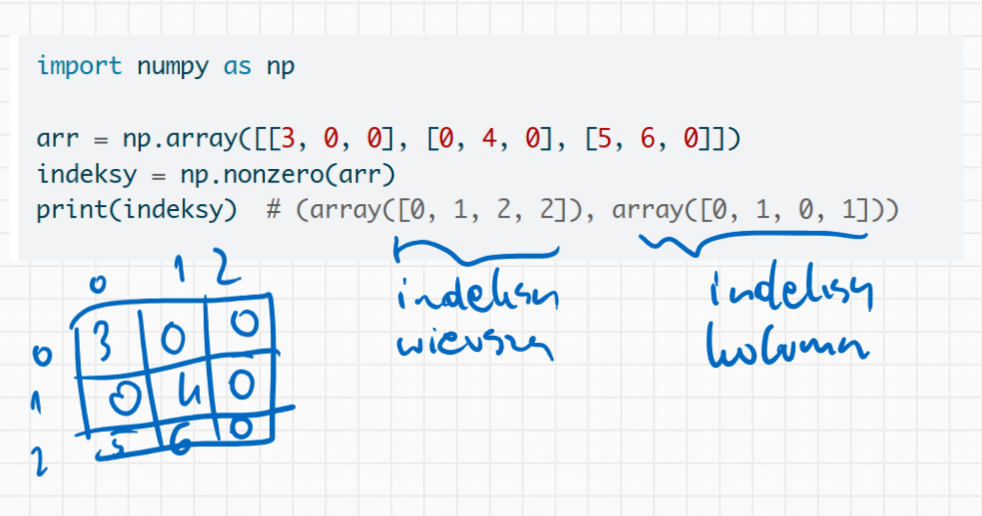
\includegraphics[keepaspectratio]{f1.png}}

\section{\texorpdfstring{Funkcja
\texttt{where()}}{Funkcja where()}}\label{funkcja-where}

Zwraca elementy wybrane z \texttt{x} lub \texttt{y} w zależności od
warunku. Jest to warunkowy selektor elementów.

\begin{Shaded}
\begin{Highlighting}[]
\ImportTok{import}\NormalTok{ numpy }\ImportTok{as}\NormalTok{ np}

\CommentTok{\# Zastąp wartości niedodatnie przez 0}
\NormalTok{arr }\OperatorTok{=}\NormalTok{ np.array([}\DecValTok{1}\NormalTok{, }\OperatorTok{{-}}\DecValTok{2}\NormalTok{, }\DecValTok{3}\NormalTok{, }\OperatorTok{{-}}\DecValTok{4}\NormalTok{, }\DecValTok{5}\NormalTok{])}
\NormalTok{wynik }\OperatorTok{=}\NormalTok{ np.where(arr }\OperatorTok{\textgreater{}} \DecValTok{0}\NormalTok{, arr, }\DecValTok{0}\NormalTok{)}
\BuiltInTok{print}\NormalTok{(wynik)  }\CommentTok{\# [1 0 3 0 5]}

\CommentTok{\# Zastosowanie w tablicy 2D}
\NormalTok{arr\_2d }\OperatorTok{=}\NormalTok{ np.array([[}\DecValTok{1}\NormalTok{, }\OperatorTok{{-}}\DecValTok{2}\NormalTok{, }\DecValTok{3}\NormalTok{], [}\OperatorTok{{-}}\DecValTok{4}\NormalTok{, }\DecValTok{5}\NormalTok{, }\OperatorTok{{-}}\DecValTok{6}\NormalTok{]])}
\NormalTok{wynik\_2d }\OperatorTok{=}\NormalTok{ np.where(arr\_2d }\OperatorTok{\textless{}} \DecValTok{0}\NormalTok{, }\OperatorTok{{-}}\DecValTok{1}\NormalTok{, arr\_2d)}
\BuiltInTok{print}\NormalTok{(wynik\_2d)}
\CommentTok{\# [[ 1 {-}1  3]}
\CommentTok{\#  [{-}1  5 {-}1]]}
\end{Highlighting}
\end{Shaded}

\begin{verbatim}
[1 0 3 0 5]
[[ 1 -1  3]
 [-1  5 -1]]
\end{verbatim}

\pandocbounded{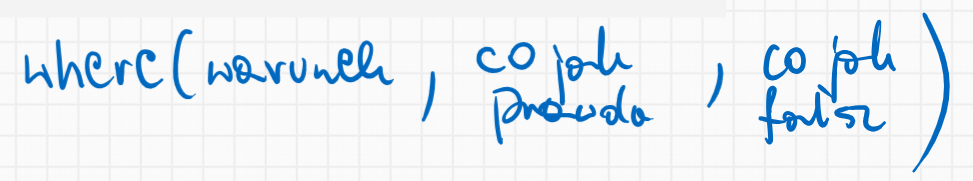
\includegraphics[keepaspectratio]{f2.png}}

\section{\texorpdfstring{Funkcje \texttt{indices()} i
\texttt{ix\_()}}{Funkcje indices() i ix\_()}}\label{funkcje-indices-i-ix_}

\subsection{\texorpdfstring{\texttt{indices()}}{indices()}}\label{indices}

Tworzy tablicę reprezentującą indeksy siatki.

\begin{Shaded}
\begin{Highlighting}[]
\ImportTok{import}\NormalTok{ numpy }\ImportTok{as}\NormalTok{ np}

\CommentTok{\# Tworzenie siatki indeksów 3x4}
\NormalTok{grid }\OperatorTok{=}\NormalTok{ np.indices((}\DecValTok{3}\NormalTok{, }\DecValTok{4}\NormalTok{))}
\BuiltInTok{print}\NormalTok{(grid.shape)  }\CommentTok{\# (2, 3, 4)}
\BuiltInTok{print}\NormalTok{(grid[}\DecValTok{0}\NormalTok{])  }\CommentTok{\# indeksy wierszy}
\CommentTok{\# [[0 0 0 0]}
\CommentTok{\#  [1 1 1 1]}
\CommentTok{\#  [2 2 2 2]]}
\BuiltInTok{print}\NormalTok{(grid[}\DecValTok{1}\NormalTok{])  }\CommentTok{\# indeksy kolumn}
\CommentTok{\# [[0 1 2 3]}
\CommentTok{\#  [0 1 2 3]}
\CommentTok{\#  [0 1 2 3]]}
\end{Highlighting}
\end{Shaded}

\begin{verbatim}
(2, 3, 4)
[[0 0 0 0]
 [1 1 1 1]
 [2 2 2 2]]
[[0 1 2 3]
 [0 1 2 3]
 [0 1 2 3]]
\end{verbatim}

\pandocbounded{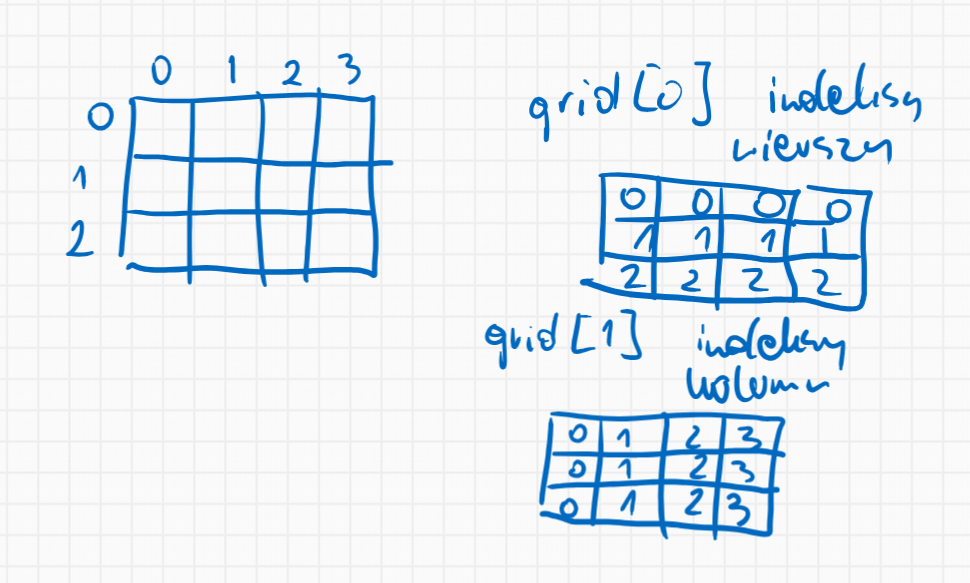
\includegraphics[keepaspectratio]{f3.png}}

\subsection{\texorpdfstring{\texttt{ix\_()}}{ix\_()}}\label{ix_}

Konstruuje otwartą siatkę z wielu sekwencji, co jest przydatne do
indeksowania wielowymiarowego.

\begin{Shaded}
\begin{Highlighting}[]
\ImportTok{import}\NormalTok{ numpy }\ImportTok{as}\NormalTok{ np}
\NormalTok{x }\OperatorTok{=}\NormalTok{ np.array([}\DecValTok{0}\NormalTok{, }\DecValTok{1}\NormalTok{, }\DecValTok{2}\NormalTok{])}
\NormalTok{y }\OperatorTok{=}\NormalTok{ np.array([}\DecValTok{3}\NormalTok{, }\DecValTok{4}\NormalTok{, }\DecValTok{5}\NormalTok{, }\DecValTok{6}\NormalTok{])}
\NormalTok{indeksy }\OperatorTok{=}\NormalTok{ np.ix\_(x, y)}

\CommentTok{\# Tworzy indeksy dla wszystkich kombinacji (0,3), (0,4), ..., (2,6)}
\BuiltInTok{print}\NormalTok{(indeksy[}\DecValTok{0}\NormalTok{].shape, indeksy[}\DecValTok{1}\NormalTok{].shape)  }\CommentTok{\# (3, 1) (1, 4)}

\CommentTok{\# Użycie do wybierania podtablicy}
\NormalTok{arr }\OperatorTok{=}\NormalTok{ np.arange(}\DecValTok{16}\NormalTok{).reshape(}\DecValTok{4}\NormalTok{, }\DecValTok{4}\NormalTok{)}
\BuiltInTok{print}\NormalTok{(arr)}
\CommentTok{\# [[ 0  1  2  3]}
\CommentTok{\#  [ 4  5  6  7]}
\CommentTok{\#  [ 8  9 10 11]}
\CommentTok{\#  [12 13 14 15]]}

\NormalTok{podtablica }\OperatorTok{=}\NormalTok{ arr[np.ix\_([}\DecValTok{0}\NormalTok{, }\DecValTok{2}\NormalTok{, }\DecValTok{3}\NormalTok{], [}\DecValTok{0}\NormalTok{, }\DecValTok{2}\NormalTok{])]}
\BuiltInTok{print}\NormalTok{(podtablica)}
\CommentTok{\# [[ 0  2]}
\CommentTok{\#  [ 8 10]}
\CommentTok{\#  [12 14]]}
\end{Highlighting}
\end{Shaded}

\begin{verbatim}
(3, 1) (1, 4)
[[ 0  1  2  3]
 [ 4  5  6  7]
 [ 8  9 10 11]
 [12 13 14 15]]
[[ 0  2]
 [ 8 10]
 [12 14]]
\end{verbatim}

\section{\texorpdfstring{\texttt{ogrid} i operacje na
siatkach}{ogrid i operacje na siatkach}}\label{ogrid-i-operacje-na-siatkach}

\texttt{ogrid} pozwala na tworzenie otwartych siatek, co jest pamięciowo
wydajniejsze niż pełne siatki.

\begin{Shaded}
\begin{Highlighting}[]
\ImportTok{import}\NormalTok{ numpy }\ImportTok{as}\NormalTok{ np}

\CommentTok{\# Siatka punktów w zakresie od {-}2 do 2 z krokiem 0.1}
\NormalTok{x, y }\OperatorTok{=}\NormalTok{ np.ogrid[}\OperatorTok{{-}}\DecValTok{2}\NormalTok{:}\DecValTok{2}\NormalTok{:}\FloatTok{0.1}\NormalTok{, }\OperatorTok{{-}}\DecValTok{2}\NormalTok{:}\DecValTok{2}\NormalTok{:}\FloatTok{0.1}\NormalTok{]}
\NormalTok{maska }\OperatorTok{=}\NormalTok{ x}\OperatorTok{**}\DecValTok{2} \OperatorTok{+}\NormalTok{ y}\OperatorTok{**}\DecValTok{2} \OperatorTok{\textless{}=} \DecValTok{1}  \CommentTok{\# Okrąg o promieniu 1}
\BuiltInTok{print}\NormalTok{(maska.shape)  }\CommentTok{\# (40, 40)}
\end{Highlighting}
\end{Shaded}

\begin{verbatim}
(40, 40)
\end{verbatim}

\section{\texorpdfstring{Funkcje \texttt{ravel\_multi\_index()} i
\texttt{unravel\_index()}}{Funkcje ravel\_multi\_index() i unravel\_index()}}\label{funkcje-ravel_multi_index-i-unravel_index}

Te funkcje konwertują między indeksami wielowymiarowymi a płaskimi.

\begin{Shaded}
\begin{Highlighting}[]
\ImportTok{import}\NormalTok{ numpy }\ImportTok{as}\NormalTok{ np}

\CommentTok{\# Konwersja indeksów wielowymiarowych na płaskie}
\NormalTok{indeksy\_wielo }\OperatorTok{=}\NormalTok{ np.array([[}\DecValTok{0}\NormalTok{, }\DecValTok{0}\NormalTok{], [}\DecValTok{1}\NormalTok{, }\DecValTok{1}\NormalTok{], [}\DecValTok{2}\NormalTok{, }\DecValTok{1}\NormalTok{]])}
\NormalTok{wymiary }\OperatorTok{=}\NormalTok{ (}\DecValTok{3}\NormalTok{, }\DecValTok{3}\NormalTok{)}
\NormalTok{indeksy\_plaskie }\OperatorTok{=}\NormalTok{ np.ravel\_multi\_index(indeksy\_wielo.T, wymiary)}
\BuiltInTok{print}\NormalTok{(indeksy\_plaskie)  }\CommentTok{\# [0 4 7]}

\CommentTok{\# Konwersja indeksów płaskich na wielowymiarowe}
\NormalTok{indeksy\_plaskie }\OperatorTok{=}\NormalTok{ np.array([}\DecValTok{0}\NormalTok{, }\DecValTok{3}\NormalTok{, }\DecValTok{8}\NormalTok{])}
\NormalTok{ksztalt }\OperatorTok{=}\NormalTok{ (}\DecValTok{3}\NormalTok{, }\DecValTok{3}\NormalTok{)}
\NormalTok{indeksy\_wielo }\OperatorTok{=}\NormalTok{ np.unravel\_index(indeksy\_plaskie, ksztalt)}
\BuiltInTok{print}\NormalTok{(indeksy\_wielo)  }\CommentTok{\# (array([0, 1, 2]), array([0, 0, 2]))}
\end{Highlighting}
\end{Shaded}

\begin{verbatim}
[0 4 7]
(array([0, 1, 2]), array([0, 0, 2]))
\end{verbatim}

\section{Indeksy diagonalne}\label{indeksy-diagonalne}

NumPy oferuje wiele funkcji do pracy z diagonalami macierzy.

\begin{Shaded}
\begin{Highlighting}[]
\ImportTok{import}\NormalTok{ numpy }\ImportTok{as}\NormalTok{ np}
\CommentTok{\# Uzyskanie indeksów głównej przekątnej}
\NormalTok{n }\OperatorTok{=} \DecValTok{4}
\NormalTok{indeksy\_diag }\OperatorTok{=}\NormalTok{ np.diag\_indices(n)}
\BuiltInTok{print}\NormalTok{(indeksy\_diag)  }\CommentTok{\# (array([0, 1, 2, 3]), array([0, 1, 2, 3]))}

\CommentTok{\# Zastosowanie do ustawienia głównej przekątnej}
\NormalTok{arr }\OperatorTok{=}\NormalTok{ np.zeros((}\DecValTok{4}\NormalTok{, }\DecValTok{4}\NormalTok{))}
\NormalTok{arr[indeksy\_diag] }\OperatorTok{=} \DecValTok{1}  \CommentTok{\# Ustawienie jedynek na głównej przekątnej}
\BuiltInTok{print}\NormalTok{(arr)}
\CommentTok{\# [[1. 0. 0. 0.]}
\CommentTok{\#  [0. 1. 0. 0.]}
\CommentTok{\#  [0. 0. 1. 0.]}
\CommentTok{\#  [0. 0. 0. 1.]]}

\CommentTok{\# Uzyskanie indeksów z istniejącej tablicy}
\NormalTok{arr2 }\OperatorTok{=}\NormalTok{ np.ones((}\DecValTok{3}\NormalTok{, }\DecValTok{3}\NormalTok{))}
\NormalTok{indeksy\_diag2 }\OperatorTok{=}\NormalTok{ np.diag\_indices\_from(arr2)}
\BuiltInTok{print}\NormalTok{(indeksy\_diag2)}
\end{Highlighting}
\end{Shaded}

\begin{verbatim}
(array([0, 1, 2, 3]), array([0, 1, 2, 3]))
[[1. 0. 0. 0.]
 [0. 1. 0. 0.]
 [0. 0. 1. 0.]
 [0. 0. 0. 1.]]
(array([0, 1, 2]), array([0, 1, 2]))
\end{verbatim}

\section{\texorpdfstring{3.1 Funkcja
\texttt{take()}}{3.1 Funkcja take()}}\label{funkcja-take}

Pobiera elementy z tablicy wzdłuż określonej osi na podstawie indeksów.

\begin{Shaded}
\begin{Highlighting}[]
\ImportTok{import}\NormalTok{ numpy }\ImportTok{as}\NormalTok{ np}

\NormalTok{arr }\OperatorTok{=}\NormalTok{ np.array([}\DecValTok{10}\NormalTok{, }\DecValTok{20}\NormalTok{, }\DecValTok{30}\NormalTok{, }\DecValTok{40}\NormalTok{, }\DecValTok{50}\NormalTok{])}
\NormalTok{indeksy }\OperatorTok{=}\NormalTok{ np.array([}\DecValTok{0}\NormalTok{, }\DecValTok{2}\NormalTok{, }\DecValTok{4}\NormalTok{])}
\NormalTok{wynik }\OperatorTok{=}\NormalTok{ np.take(arr, indeksy)}
\BuiltInTok{print}\NormalTok{(wynik)  }\CommentTok{\# [10 30 50]}

\CommentTok{\# W tablicach wielowymiarowych możemy wybrać oś}
\NormalTok{arr\_2d }\OperatorTok{=}\NormalTok{ np.array([[}\DecValTok{1}\NormalTok{, }\DecValTok{2}\NormalTok{, }\DecValTok{3}\NormalTok{], [}\DecValTok{4}\NormalTok{, }\DecValTok{5}\NormalTok{, }\DecValTok{6}\NormalTok{], [}\DecValTok{7}\NormalTok{, }\DecValTok{8}\NormalTok{, }\DecValTok{9}\NormalTok{]])}
\NormalTok{indeksy\_wierszy }\OperatorTok{=}\NormalTok{ np.array([}\DecValTok{0}\NormalTok{, }\DecValTok{2}\NormalTok{])}
\NormalTok{wynik\_2d }\OperatorTok{=}\NormalTok{ np.take(arr\_2d, indeksy\_wierszy, axis}\OperatorTok{=}\DecValTok{0}\NormalTok{)}
\BuiltInTok{print}\NormalTok{(wynik\_2d)}
\CommentTok{\# [[1 2 3]}
\CommentTok{\#  [7 8 9]]}
\end{Highlighting}
\end{Shaded}

\begin{verbatim}
[10 30 50]
[[1 2 3]
 [7 8 9]]
\end{verbatim}

\#\#Funkcja \texttt{take\_along\_axis()}

Pobiera wartości z tablicy poprzez dopasowanie 1D indeksu i fragmentów
danych. Jest bezpieczna dla duplikatów indeksów.

\begin{Shaded}
\begin{Highlighting}[]
\ImportTok{import}\NormalTok{ numpy }\ImportTok{as}\NormalTok{ np}

\NormalTok{arr }\OperatorTok{=}\NormalTok{ np.array([[}\DecValTok{10}\NormalTok{, }\DecValTok{30}\NormalTok{, }\DecValTok{20}\NormalTok{], [}\DecValTok{60}\NormalTok{, }\DecValTok{40}\NormalTok{, }\DecValTok{50}\NormalTok{]])}
\NormalTok{indeksy\_kolejnosc }\OperatorTok{=}\NormalTok{ np.argsort(arr, axis}\OperatorTok{=}\DecValTok{1}\NormalTok{)}
\NormalTok{wynik }\OperatorTok{=}\NormalTok{ np.take\_along\_axis(arr, indeksy\_kolejnosc, axis}\OperatorTok{=}\DecValTok{1}\NormalTok{)}
\BuiltInTok{print}\NormalTok{(wynik)}
\CommentTok{\# [[10 20 30]}
\CommentTok{\#  [40 50 60]]}
\end{Highlighting}
\end{Shaded}

\begin{verbatim}
[[10 20 30]
 [40 50 60]]
\end{verbatim}

\section{\texorpdfstring{Funkcja
\texttt{choose()}}{Funkcja choose()}}\label{funkcja-choose}

Konstruuje tablicę wybierając elementy z listy tablic.

\begin{Shaded}
\begin{Highlighting}[]
\ImportTok{import}\NormalTok{ numpy }\ImportTok{as}\NormalTok{ np}

\NormalTok{opcje }\OperatorTok{=}\NormalTok{ [np.array([}\DecValTok{0}\NormalTok{, }\DecValTok{1}\NormalTok{, }\DecValTok{2}\NormalTok{, }\DecValTok{3}\NormalTok{]),}
\NormalTok{         np.array([}\DecValTok{10}\NormalTok{, }\DecValTok{11}\NormalTok{, }\DecValTok{12}\NormalTok{, }\DecValTok{13}\NormalTok{]),}
\NormalTok{         np.array([}\DecValTok{20}\NormalTok{, }\DecValTok{21}\NormalTok{, }\DecValTok{22}\NormalTok{, }\DecValTok{23}\NormalTok{])]}
\NormalTok{indeksy }\OperatorTok{=}\NormalTok{ np.array([}\DecValTok{0}\NormalTok{, }\DecValTok{2}\NormalTok{, }\DecValTok{1}\NormalTok{, }\DecValTok{0}\NormalTok{])  }\CommentTok{\# Wybiera z której tablicy opcji wziąć element}
\NormalTok{wynik }\OperatorTok{=}\NormalTok{ np.choose(indeksy, opcje)}
\BuiltInTok{print}\NormalTok{(wynik)  }\CommentTok{\# [ 0 21 12  3]}
\end{Highlighting}
\end{Shaded}

\begin{verbatim}
[ 0 21 12  3]
\end{verbatim}

\section{\texorpdfstring{Funkcja
\texttt{compress()}}{Funkcja compress()}}\label{funkcja-compress}

Zwraca wybrane elementy tablicy wzdłuż określonej osi.

\begin{Shaded}
\begin{Highlighting}[]
\ImportTok{import}\NormalTok{ numpy }\ImportTok{as}\NormalTok{ np}
\NormalTok{arr }\OperatorTok{=}\NormalTok{ np.array([[}\DecValTok{1}\NormalTok{, }\DecValTok{2}\NormalTok{, }\DecValTok{3}\NormalTok{], [}\DecValTok{4}\NormalTok{, }\DecValTok{5}\NormalTok{, }\DecValTok{6}\NormalTok{]])}
\NormalTok{maska }\OperatorTok{=}\NormalTok{ np.array([}\VariableTok{True}\NormalTok{, }\VariableTok{False}\NormalTok{, }\VariableTok{True}\NormalTok{])}
\NormalTok{wynik }\OperatorTok{=}\NormalTok{ np.compress(maska, arr, axis}\OperatorTok{=}\DecValTok{1}\NormalTok{)}
\BuiltInTok{print}\NormalTok{(wynik)}
\CommentTok{\# [[1 3]}
\CommentTok{\#  [4 6]]}
\end{Highlighting}
\end{Shaded}

\begin{verbatim}
[[1 3]
 [4 6]]
\end{verbatim}

\section{\texorpdfstring{Funkcje \texttt{diag()} i
\texttt{diagonal()}}{Funkcje diag() i diagonal()}}\label{funkcje-diag-i-diagonal}

Funkcje do pracy z przekątnymi.

\begin{Shaded}
\begin{Highlighting}[]
\ImportTok{import}\NormalTok{ numpy }\ImportTok{as}\NormalTok{ np}

\CommentTok{\# Tworzenie tablicy diagonalnej}
\NormalTok{diag\_arr }\OperatorTok{=}\NormalTok{ np.diag([}\DecValTok{1}\NormalTok{, }\DecValTok{2}\NormalTok{, }\DecValTok{3}\NormalTok{, }\DecValTok{4}\NormalTok{])}
\BuiltInTok{print}\NormalTok{(diag\_arr)}
\CommentTok{\# [[1 0 0 0]}
\CommentTok{\#  [0 2 0 0]}
\CommentTok{\#  [0 0 3 0]}
\CommentTok{\#  [0 0 0 4]]}

\CommentTok{\# Pobieranie diagonali z tablicy}
\NormalTok{arr }\OperatorTok{=}\NormalTok{ np.array([[}\DecValTok{1}\NormalTok{, }\DecValTok{2}\NormalTok{, }\DecValTok{3}\NormalTok{], [}\DecValTok{4}\NormalTok{, }\DecValTok{5}\NormalTok{, }\DecValTok{6}\NormalTok{], [}\DecValTok{7}\NormalTok{, }\DecValTok{8}\NormalTok{, }\DecValTok{9}\NormalTok{]])}
\NormalTok{diag }\OperatorTok{=}\NormalTok{ np.diag(arr)}
\BuiltInTok{print}\NormalTok{(diag)  }\CommentTok{\# [1 5 9]}

\CommentTok{\# Pobieranie przekątnej przesuniętej o 1}
\NormalTok{diag\_offset }\OperatorTok{=}\NormalTok{ np.diagonal(arr, offset}\OperatorTok{=}\DecValTok{1}\NormalTok{)}
\BuiltInTok{print}\NormalTok{(diag\_offset)  }\CommentTok{\# [2 6]}
\end{Highlighting}
\end{Shaded}

\begin{verbatim}
[[1 0 0 0]
 [0 2 0 0]
 [0 0 3 0]
 [0 0 0 4]]
[1 5 9]
[2 6]
\end{verbatim}

\section{\texorpdfstring{Funkcja
\texttt{select()}}{Funkcja select()}}\label{funkcja-select}

Zwraca tablicę zbudowaną z elementów z listy opcji, w zależności od
warunków.

\begin{Shaded}
\begin{Highlighting}[]
\ImportTok{import}\NormalTok{ numpy }\ImportTok{as}\NormalTok{ np}

\NormalTok{arr }\OperatorTok{=}\NormalTok{ np.array([[}\DecValTok{1}\NormalTok{, }\DecValTok{2}\NormalTok{, }\DecValTok{3}\NormalTok{], [}\DecValTok{4}\NormalTok{, }\DecValTok{5}\NormalTok{, }\DecValTok{6}\NormalTok{], [}\DecValTok{7}\NormalTok{, }\DecValTok{8}\NormalTok{, }\DecValTok{9}\NormalTok{]])}
\NormalTok{warunki }\OperatorTok{=}\NormalTok{ [arr }\OperatorTok{\textless{}} \DecValTok{3}\NormalTok{, arr }\OperatorTok{\textless{}} \DecValTok{6}\NormalTok{, arr }\OperatorTok{\textless{}} \DecValTok{9}\NormalTok{]}
\NormalTok{opcje }\OperatorTok{=}\NormalTok{ [}\DecValTok{100}\NormalTok{, }\DecValTok{200}\NormalTok{, }\DecValTok{300}\NormalTok{]}
\NormalTok{wynik }\OperatorTok{=}\NormalTok{ np.select(warunki, opcje, default}\OperatorTok{=}\DecValTok{400}\NormalTok{)}
\BuiltInTok{print}\NormalTok{(wynik)}
\CommentTok{\# [[100 100 200]}
\CommentTok{\#  [200 200 300]}
\CommentTok{\#  [300 300 400]]}
\end{Highlighting}
\end{Shaded}

\begin{verbatim}
[[100 100 200]
 [200 200 300]
 [300 300 400]]
\end{verbatim}

\section{\texorpdfstring{Funkcja
\texttt{place()}}{Funkcja place()}}\label{funkcja-place}

Zmienia elementy tablicy na podstawie maski i podanych wartości.

\begin{Shaded}
\begin{Highlighting}[]
\ImportTok{import}\NormalTok{ numpy }\ImportTok{as}\NormalTok{ np}

\NormalTok{arr }\OperatorTok{=}\NormalTok{ np.arange(}\DecValTok{5}\NormalTok{)}
\NormalTok{maska }\OperatorTok{=}\NormalTok{ np.array([}\VariableTok{True}\NormalTok{, }\VariableTok{False}\NormalTok{, }\VariableTok{True}\NormalTok{, }\VariableTok{False}\NormalTok{, }\VariableTok{True}\NormalTok{])}
\NormalTok{np.place(arr, maska, [}\OperatorTok{{-}}\DecValTok{1}\NormalTok{, }\OperatorTok{{-}}\DecValTok{2}\NormalTok{, }\OperatorTok{{-}}\DecValTok{3}\NormalTok{])  }\CommentTok{\# Cyklicznie używa wartości [{-}1, {-}2, {-}3]}
\BuiltInTok{print}\NormalTok{(arr)  }\CommentTok{\# [{-}1  1 {-}2  3 {-}3]}
\end{Highlighting}
\end{Shaded}

\begin{verbatim}
[-1  1 -2  3 -3]
\end{verbatim}

\section{\texorpdfstring{Funkcja
\texttt{put()}}{Funkcja put()}}\label{funkcja-put}

Zastępuje określone elementy tablicy podanymi wartościami.

\begin{Shaded}
\begin{Highlighting}[]
\ImportTok{import}\NormalTok{ numpy }\ImportTok{as}\NormalTok{ np}

\NormalTok{arr }\OperatorTok{=}\NormalTok{ np.arange(}\DecValTok{5}\NormalTok{)}
\NormalTok{indeksy }\OperatorTok{=}\NormalTok{ [}\DecValTok{0}\NormalTok{, }\DecValTok{2}\NormalTok{, }\DecValTok{4}\NormalTok{]}
\NormalTok{np.put(arr, indeksy, [}\DecValTok{10}\NormalTok{, }\DecValTok{20}\NormalTok{, }\DecValTok{30}\NormalTok{])}
\BuiltInTok{print}\NormalTok{(arr)  }\CommentTok{\# [10  1 20  3 30]}
\end{Highlighting}
\end{Shaded}

\begin{verbatim}
[10  1 20  3 30]
\end{verbatim}

\section{\texorpdfstring{Funkcja
\texttt{put\_along\_axis()}}{Funkcja put\_along\_axis()}}\label{funkcja-put_along_axis}

Umieszcza wartości w tablicy docelowej, dopasowując 1D indeks i
fragmenty danych wzdłuż określonej osi.

\begin{Shaded}
\begin{Highlighting}[]
\ImportTok{import}\NormalTok{ numpy }\ImportTok{as}\NormalTok{ np}

\NormalTok{arr }\OperatorTok{=}\NormalTok{ np.array([[}\DecValTok{10}\NormalTok{, }\DecValTok{30}\NormalTok{, }\DecValTok{20}\NormalTok{], [}\DecValTok{60}\NormalTok{, }\DecValTok{40}\NormalTok{, }\DecValTok{50}\NormalTok{]])}
\NormalTok{indeksy }\OperatorTok{=}\NormalTok{ np.argmin(arr, axis}\OperatorTok{=}\DecValTok{1}\NormalTok{)}
\NormalTok{indeksy }\OperatorTok{=}\NormalTok{ np.expand\_dims(indeksy, axis}\OperatorTok{=}\DecValTok{1}\NormalTok{)  }\CommentTok{\# Przekształć do kształtu (2, 1)}
\NormalTok{np.put\_along\_axis(arr, indeksy, }\DecValTok{99}\NormalTok{, axis}\OperatorTok{=}\DecValTok{1}\NormalTok{)}
\BuiltInTok{print}\NormalTok{(arr)}
\CommentTok{\# [[99 30 20]}
\CommentTok{\#  [60 40 99]]}
\end{Highlighting}
\end{Shaded}

\begin{verbatim}
[[99 30 20]
 [60 99 50]]
\end{verbatim}

\section{\texorpdfstring{Funkcja
\texttt{putmask()}}{Funkcja putmask()}}\label{funkcja-putmask}

Zmienia elementy tablicy na podstawie warunku i podanych wartości.

\begin{Shaded}
\begin{Highlighting}[]
\ImportTok{import}\NormalTok{ numpy }\ImportTok{as}\NormalTok{ np}

\NormalTok{arr }\OperatorTok{=}\NormalTok{ np.arange(}\DecValTok{5}\NormalTok{)}
\NormalTok{maska }\OperatorTok{=}\NormalTok{ np.array([}\VariableTok{True}\NormalTok{, }\VariableTok{False}\NormalTok{, }\VariableTok{True}\NormalTok{, }\VariableTok{False}\NormalTok{, }\VariableTok{True}\NormalTok{])}
\NormalTok{np.putmask(arr, maska, [}\OperatorTok{{-}}\DecValTok{1}\NormalTok{, }\OperatorTok{{-}}\DecValTok{2}\NormalTok{, }\OperatorTok{{-}}\DecValTok{3}\NormalTok{])  }\CommentTok{\# Cyklicznie używa wartości}
\BuiltInTok{print}\NormalTok{(arr)  }\CommentTok{\# [{-}1  1 {-}2  3 {-}3]}
\end{Highlighting}
\end{Shaded}

\begin{verbatim}
[-1  1 -3  3 -2]
\end{verbatim}

\section{\texorpdfstring{Funkcja
\texttt{fill\_diagonal()}}{Funkcja fill\_diagonal()}}\label{funkcja-fill_diagonal}

Wypełnia główną przekątną tablicy podaną wartością.

\begin{Shaded}
\begin{Highlighting}[]
\ImportTok{import}\NormalTok{ numpy }\ImportTok{as}\NormalTok{ np}

\NormalTok{arr }\OperatorTok{=}\NormalTok{ np.zeros((}\DecValTok{4}\NormalTok{, }\DecValTok{4}\NormalTok{))}
\NormalTok{np.fill\_diagonal(arr, }\DecValTok{5}\NormalTok{)}
\BuiltInTok{print}\NormalTok{(arr)}
\CommentTok{\# [[5. 0. 0. 0.]}
\CommentTok{\#  [0. 5. 0. 0.]}
\CommentTok{\#  [0. 0. 5. 0.]}
\CommentTok{\#  [0. 0. 0. 5.]]}

\NormalTok{arr\_rect }\OperatorTok{=}\NormalTok{ np.zeros((}\DecValTok{4}\NormalTok{, }\DecValTok{4}\NormalTok{, }\DecValTok{4}\NormalTok{))}
\NormalTok{np.fill\_diagonal(arr\_rect, }\DecValTok{9}\NormalTok{)}
\BuiltInTok{print}\NormalTok{(arr\_rect[}\DecValTok{0}\NormalTok{])  }\CommentTok{\# Wypełnia przekątną w każdym "plasterku" 3D tablicy}
\end{Highlighting}
\end{Shaded}

\begin{verbatim}
[[5. 0. 0. 0.]
 [0. 5. 0. 0.]
 [0. 0. 5. 0.]
 [0. 0. 0. 5.]]
[[9. 0. 0. 0.]
 [0. 0. 0. 0.]
 [0. 0. 0. 0.]
 [0. 0. 0. 0.]]
\end{verbatim}

\chapter{Numpy - inne}\label{numpy---inne}

\section{Stałe}\label{staux142e}

\texttt{NumPy} dostarcza kilka znanych stałych matematycznych, które
mogą być przydatne w obliczeniach naukowych i inżynierskich. Wbudowane
stałe takie jak liczba Pi czy podstawa logarytmu naturalnego \texttt{e}
ułatwiają pisanie czytelnego i zwięzłego kodu.

\begin{enumerate}
\def\labelenumi{\arabic{enumi}.}
\tightlist
\item
  \textbf{\texttt{numpy.pi}}

  \begin{itemize}
  \tightlist
  \item
    Reprezentuje liczbę Pi (π) z dużą dokładnością.\\
  \item
    Pi to stosunek obwodu okręgu do jego średnicy.\\
  \item
    W przybliżeniu: \texttt{3.141592653589793}
  \end{itemize}
\item
  \textbf{\texttt{numpy.e}}

  \begin{itemize}
  \tightlist
  \item
    Reprezentuje podstawę logarytmu naturalnego, \texttt{e}.\\
  \item
    \texttt{e} jest wykorzystywane w wielu dziedzinach, takich jak
    analiza matematyczna, probabilistyka, statystyka.\\
  \item
    W przybliżeniu: \texttt{2.718281828459045}
  \end{itemize}
\item
  \textbf{\texttt{numpy.eulergamma}}

  \begin{itemize}
  \tightlist
  \item
    Reprezentuje stałą Eulera-Mascheroniego, zwykle oznaczaną jako γ
    (gamma).
  \item
    Pojawia się w analizie matematycznej, szczególnie w teorii liczb i
    badaniu szeregów harmonicznych.
  \item
    W przybliżeniu: \texttt{0.5772156649015329}
  \end{itemize}
\end{enumerate}

\begin{Shaded}
\begin{Highlighting}[]
\ImportTok{import}\NormalTok{ numpy }\ImportTok{as}\NormalTok{ np}

\CommentTok{\# Promień koła}
\NormalTok{r }\OperatorTok{=} \FloatTok{5.0}

\CommentTok{\# Obwód koła: 2 * π * r}
\NormalTok{obwod }\OperatorTok{=} \DecValTok{2} \OperatorTok{*}\NormalTok{ np.pi }\OperatorTok{*}\NormalTok{ r}
\BuiltInTok{print}\NormalTok{(}\StringTok{"Obwód koła:"}\NormalTok{, obwod)}

\CommentTok{\# Pole koła: π * r\^{}2}
\NormalTok{pole }\OperatorTok{=}\NormalTok{ np.pi }\OperatorTok{*}\NormalTok{ r}\OperatorTok{**}\DecValTok{2}
\BuiltInTok{print}\NormalTok{(}\StringTok{"Pole koła:"}\NormalTok{, pole)}
\end{Highlighting}
\end{Shaded}

\begin{verbatim}
Obwód koła: 31.41592653589793
Pole koła: 78.53981633974483
\end{verbatim}

\begin{Shaded}
\begin{Highlighting}[]
\ImportTok{import}\NormalTok{ numpy }\ImportTok{as}\NormalTok{ np}

\CommentTok{\# Przykładowy punkt x}
\NormalTok{x }\OperatorTok{=} \FloatTok{1.0}

\CommentTok{\# Wartość funkcji e\^{}x}
\NormalTok{exp\_value }\OperatorTok{=}\NormalTok{ np.e}\OperatorTok{**}\NormalTok{x}
\BuiltInTok{print}\NormalTok{(}\StringTok{"e\^{}x dla x=1:"}\NormalTok{, exp\_value)}

\CommentTok{\# Porównanie z funkcją np.exp}
\NormalTok{exp\_compare }\OperatorTok{=}\NormalTok{ np.exp(x)}
\BuiltInTok{print}\NormalTok{(}\StringTok{"Porównanie z np.exp(1):"}\NormalTok{, exp\_compare)}
\end{Highlighting}
\end{Shaded}

\begin{verbatim}
e^x dla x=1: 2.718281828459045
Porównanie z np.exp(1): 2.718281828459045
\end{verbatim}

\section{\texorpdfstring{\texttt{numpy.inf}}{numpy.inf}}\label{numpy.inf}

\begin{itemize}
\tightlist
\item
  \textbf{Opis}: \texttt{np.inf} reprezentuje wartość nieskończoną
  (∞).\\
\item
  Często pojawia się w obliczeniach, gdy wartość danego wyrażenia dąży
  do nieskończoności (np. dzielenie przez zero, pewne limity, itp.).\\
\item
  Przykładowo, \texttt{1.0\ /\ 0.0} zwróci ostrzeżenie i w konsekwencji
  może dać wartość \texttt{inf}.
\end{itemize}

\begin{Shaded}
\begin{Highlighting}[]
\ImportTok{import}\NormalTok{ numpy }\ImportTok{as}\NormalTok{ np}

\CommentTok{\# Zastosowanie w tworzeniu masek logicznych}
\NormalTok{arr }\OperatorTok{=}\NormalTok{ np.array([}\DecValTok{1}\NormalTok{, }\DecValTok{2}\NormalTok{, np.inf, }\DecValTok{4}\NormalTok{, }\DecValTok{5}\NormalTok{])}
\NormalTok{mask }\OperatorTok{=}\NormalTok{ np.isinf(arr)}
\BuiltInTok{print}\NormalTok{(}\StringTok{"Maska elementów o wartości inf:"}\NormalTok{, mask)}
\end{Highlighting}
\end{Shaded}

\begin{verbatim}
Maska elementów o wartości inf: [False False  True False False]
\end{verbatim}

\section{\texorpdfstring{\texttt{numpy.nan}}{numpy.nan}}\label{numpy.nan}

\begin{itemize}
\tightlist
\item
  \textbf{Opis}: \texttt{np.nan} oznacza ``Not a Number'' (NaN), czyli
  wartość nieokreśloną lub niereprezentowalną w systemie liczbowym.\\
\item
  Pojawia się, gdy wynik operacji numerycznej jest nieokreślony, np.
  \texttt{0.0/0.0}, \texttt{inf\ -\ inf} lub przy błędach wczytywania
  danych.\\
\item
  Operacje arytmetyczne z \texttt{nan} zazwyczaj również zwracają
  \texttt{nan}.
\end{itemize}

\begin{Shaded}
\begin{Highlighting}[]
\ImportTok{import}\NormalTok{ numpy }\ImportTok{as}\NormalTok{ np}

\CommentTok{\# Zamiana wartości nan w tablicy}
\NormalTok{data }\OperatorTok{=}\NormalTok{ np.array([}\DecValTok{1}\NormalTok{, }\DecValTok{2}\NormalTok{, np.nan, }\DecValTok{4}\NormalTok{, np.nan])}
\BuiltInTok{print}\NormalTok{(}\StringTok{"Oryginalne dane:"}\NormalTok{, data)}

\CommentTok{\# Wypełnienie wartości nan zerem}
\NormalTok{data\_no\_nan }\OperatorTok{=}\NormalTok{ np.nan\_to\_num(data, nan}\OperatorTok{=}\FloatTok{0.0}\NormalTok{)}
\BuiltInTok{print}\NormalTok{(}\StringTok{"Dane bez nan:"}\NormalTok{, data\_no\_nan)}
\end{Highlighting}
\end{Shaded}

\begin{verbatim}
Oryginalne dane: [ 1.  2. nan  4. nan]
Dane bez nan: [1. 2. 0. 4. 0.]
\end{verbatim}

\section{\texorpdfstring{\texttt{numpy.newaxis}}{numpy.newaxis}}\label{numpy.newaxis}

\begin{itemize}
\tightlist
\item
  \textbf{Opis}: \texttt{np.newaxis} jest specjalną ``stałą''/obiektem
  służącym do zmiany wymiarów tablic przez zwiększenie ich liczby
  wymiarów o 1.
\end{itemize}

\begin{Shaded}
\begin{Highlighting}[]
\ImportTok{import}\NormalTok{ numpy }\ImportTok{as}\NormalTok{ np}

\CommentTok{\# Mamy tablicę 1D}
\NormalTok{vec }\OperatorTok{=}\NormalTok{ np.array([}\DecValTok{1}\NormalTok{, }\DecValTok{2}\NormalTok{, }\DecValTok{3}\NormalTok{, }\DecValTok{4}\NormalTok{])}
\BuiltInTok{print}\NormalTok{(}\StringTok{"Oryginalna tablica:"}\NormalTok{, vec, }\StringTok{"Kształt:"}\NormalTok{, vec.shape)}

\CommentTok{\# Dodajemy nowy wymiar jako wymiar wierszy}
\NormalTok{vec\_as\_col }\OperatorTok{=}\NormalTok{ vec[:, np.newaxis]}
\BuiltInTok{print}\NormalTok{(}\StringTok{"Tablica jako kolumna:}\CharTok{\textbackslash{}n}\StringTok{"}\NormalTok{, vec\_as\_col, }\StringTok{"Kształt:"}\NormalTok{, vec\_as\_col.shape)}

\CommentTok{\# Dodawanie wymiaru na początku}
\NormalTok{vec\_as\_row }\OperatorTok{=}\NormalTok{ vec[np.newaxis, :]}
\BuiltInTok{print}\NormalTok{(}\StringTok{"Tablica jako wiersz:}\CharTok{\textbackslash{}n}\StringTok{"}\NormalTok{, vec\_as\_row, }\StringTok{"Kształt:"}\NormalTok{, vec\_as\_row.shape)}

\CommentTok{\# Kolejny przykład: dodanie wymiaru by z łatwością broadcastować operacje}
\NormalTok{a }\OperatorTok{=}\NormalTok{ np.array([}\DecValTok{10}\NormalTok{, }\DecValTok{20}\NormalTok{, }\DecValTok{30}\NormalTok{])}
\NormalTok{b }\OperatorTok{=}\NormalTok{ np.array([}\DecValTok{1}\NormalTok{, }\DecValTok{2}\NormalTok{])}
\CommentTok{\# Bez nowego wymiaru próba dodania a do b się nie powiedzie, }
\CommentTok{\# bo kształty nie są kompatybilne.}
\CommentTok{\# Z nowym wymiarem a ma kształt (3,1), a b (2,), co pozwala na broadcast}
\NormalTok{sum\_matrix }\OperatorTok{=}\NormalTok{ a[:, np.newaxis] }\OperatorTok{+}\NormalTok{ b}
\BuiltInTok{print}\NormalTok{(}\StringTok{"Operacja z broadcast:}\CharTok{\textbackslash{}n}\StringTok{"}\NormalTok{, sum\_matrix)}
\end{Highlighting}
\end{Shaded}

\begin{verbatim}
Oryginalna tablica: [1 2 3 4] Kształt: (4,)
Tablica jako kolumna:
 [[1]
 [2]
 [3]
 [4]] Kształt: (4, 1)
Tablica jako wiersz:
 [[1 2 3 4]] Kształt: (1, 4)
Operacja z broadcast:
 [[11 12]
 [21 22]
 [31 32]]
\end{verbatim}

\section{Statystyka i agregacja}\label{statystyka-i-agregacja}

\begin{longtable}[]{@{}
  >{\raggedright\arraybackslash}p{(\linewidth - 2\tabcolsep) * \real{0.2558}}
  >{\raggedright\arraybackslash}p{(\linewidth - 2\tabcolsep) * \real{0.7442}}@{}}
\toprule\noalign{}
\begin{minipage}[b]{\linewidth}\raggedright
Funkcja
\end{minipage} & \begin{minipage}[b]{\linewidth}\raggedright
Opis
\end{minipage} \\
\midrule\noalign{}
\endhead
\bottomrule\noalign{}
\endlastfoot
np.mean & Średnia wszystkich wartości w tablicy. \\
np.std & Odchylenie standardowe. \\
np.var & Wariancja. \\
np.sum & Suma wszystkich elementów. \\
np.prod & Iloczyn wszystkich elementów. \\
np.cumsum & Skumulowana suma wszystkich elementów. \\
np.cumprod & Skumulowany iloczyn wszystkich elementów. \\
np.min,np.max & Minimalna/maksymalna wartość w tablicy. \\
np.argmin, np.argmax & Indeks minimalnej/maksymalnej wartości w
tablicy. \\
np.all & Sprawdza czy wszystki elementy są różne od zera. \\
np.any & Sprawdza czy co najmniej jeden z elementów jest różny od
zera. \\
\end{longtable}

\part{Eksploracja danych}

\chapter{Etapy eksploracji danych}\label{etapy-eksploracji-danych}

\begin{itemize}
\tightlist
\item
  \textbf{Zbieranie danych}:

  \begin{itemize}
  \tightlist
  \item
    Zebranie danych z różnych źródeł (bazy danych, pliki CSV, API,
    itd.).
  \end{itemize}
\item
  \textbf{Zrozumienie danych}:

  \begin{itemize}
  \tightlist
  \item
    Analiza struktury danych, typów danych i ich znaczenia.
  \item
    Eksploracja wstępnych zależności i trendów.
  \end{itemize}
\item
  \textbf{Czyszczenie danych}:

  \begin{itemize}
  \tightlist
  \item
    Usuwanie braków, błędów i anomalii w danych.
  \item
    Obsługa brakujących wartości i duplikatów.
  \end{itemize}
\item
  \textbf{Transformacja danych}:

  \begin{itemize}
  \tightlist
  \item
    Normalizacja, standaryzacja, kodowanie zmiennych kategorycznych.
  \item
    Tworzenie nowych zmiennych (cech).
  \end{itemize}
\item
  \textbf{Redukcja danych}:

  \begin{itemize}
  \tightlist
  \item
    Selekcja istotnych cech lub zmniejszenie wymiarowości danych (np.
    PCA).
  \end{itemize}
\end{itemize}

\part{Pandas}

\chapter{Pandas - start}\label{pandas---start}

Pandas jest biblioteką Pythona służącą do analizy i manipulowania danymi

\section{Import:}\label{import}

\begin{Shaded}
\begin{Highlighting}[]
\ImportTok{import}\NormalTok{ pandas }\ImportTok{as}\NormalTok{ pd}
\end{Highlighting}
\end{Shaded}

\section{Podstawowe byty}\label{podstawowe-byty}

Seria - Series

\pandocbounded{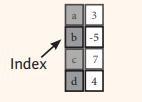
\includegraphics[keepaspectratio]{51.png}}

\begin{center}\rule{0.5\linewidth}{0.5pt}\end{center}

Ramka danych - DataFrame

\pandocbounded{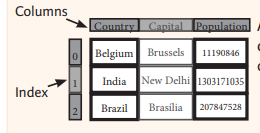
\includegraphics[keepaspectratio]{52.png}}

\begin{Shaded}
\begin{Highlighting}[]
\ImportTok{import}\NormalTok{ pandas }\ImportTok{as}\NormalTok{ pd}

\NormalTok{s }\OperatorTok{=}\NormalTok{ pd.Series([}\DecValTok{3}\NormalTok{, }\OperatorTok{{-}}\DecValTok{5}\NormalTok{, }\DecValTok{7}\NormalTok{, }\DecValTok{4}\NormalTok{])}
\BuiltInTok{print}\NormalTok{(s)}
\BuiltInTok{print}\NormalTok{(}\StringTok{"values"}\NormalTok{)}
\BuiltInTok{print}\NormalTok{(s.to\_numpy())}
\BuiltInTok{print}\NormalTok{(}\BuiltInTok{type}\NormalTok{(s.to\_numpy()))}
\BuiltInTok{print}\NormalTok{(s.index)}
\BuiltInTok{print}\NormalTok{(}\BuiltInTok{type}\NormalTok{(s.index))}
\end{Highlighting}
\end{Shaded}

\begin{verbatim}
0    3
1   -5
2    7
3    4
dtype: int64
values
[ 3 -5  7  4]
<class 'numpy.ndarray'>
RangeIndex(start=0, stop=4, step=1)
<class 'pandas.core.indexes.range.RangeIndex'>
\end{verbatim}

\begin{Shaded}
\begin{Highlighting}[]
\ImportTok{import}\NormalTok{ pandas }\ImportTok{as}\NormalTok{ pd}
\ImportTok{import}\NormalTok{ numpy }\ImportTok{as}\NormalTok{ np}

\NormalTok{s }\OperatorTok{=}\NormalTok{ pd.Series([}\DecValTok{3}\NormalTok{, }\OperatorTok{{-}}\DecValTok{5}\NormalTok{, }\DecValTok{7}\NormalTok{, }\DecValTok{4}\NormalTok{], index}\OperatorTok{=}\NormalTok{[}\StringTok{\textquotesingle{}a\textquotesingle{}}\NormalTok{, }\StringTok{\textquotesingle{}b\textquotesingle{}}\NormalTok{, }\StringTok{\textquotesingle{}c\textquotesingle{}}\NormalTok{, }\StringTok{\textquotesingle{}d\textquotesingle{}}\NormalTok{])}
\BuiltInTok{print}\NormalTok{(s)}
\BuiltInTok{print}\NormalTok{(s[}\StringTok{\textquotesingle{}b\textquotesingle{}}\NormalTok{])}
\NormalTok{s[}\StringTok{\textquotesingle{}b\textquotesingle{}}\NormalTok{] }\OperatorTok{=} \DecValTok{8}
\BuiltInTok{print}\NormalTok{(s)}
\BuiltInTok{print}\NormalTok{(s[s }\OperatorTok{\textgreater{}} \DecValTok{5}\NormalTok{])}
\BuiltInTok{print}\NormalTok{(s }\OperatorTok{*} \DecValTok{2}\NormalTok{)}
\BuiltInTok{print}\NormalTok{(np.sin(s))}
\end{Highlighting}
\end{Shaded}

\begin{verbatim}
a    3
b   -5
c    7
d    4
dtype: int64
-5
a    3
b    8
c    7
d    4
dtype: int64
b    8
c    7
dtype: int64
a     6
b    16
c    14
d     8
dtype: int64
a    0.141120
b    0.989358
c    0.656987
d   -0.756802
dtype: float64
\end{verbatim}

\begin{Shaded}
\begin{Highlighting}[]
\ImportTok{import}\NormalTok{ pandas }\ImportTok{as}\NormalTok{ pd}

\NormalTok{d }\OperatorTok{=}\NormalTok{ \{}\StringTok{\textquotesingle{}key1\textquotesingle{}}\NormalTok{: }\DecValTok{350}\NormalTok{, }\StringTok{\textquotesingle{}key2\textquotesingle{}}\NormalTok{: }\DecValTok{700}\NormalTok{, }\StringTok{\textquotesingle{}key3\textquotesingle{}}\NormalTok{: }\DecValTok{70}\NormalTok{\}}
\NormalTok{s }\OperatorTok{=}\NormalTok{ pd.Series(d)}
\BuiltInTok{print}\NormalTok{(s)}
\end{Highlighting}
\end{Shaded}

\begin{verbatim}
key1    350
key2    700
key3     70
dtype: int64
\end{verbatim}

\begin{Shaded}
\begin{Highlighting}[]
\ImportTok{import}\NormalTok{ pandas }\ImportTok{as}\NormalTok{ pd}

\NormalTok{d }\OperatorTok{=}\NormalTok{ \{}\StringTok{\textquotesingle{}key1\textquotesingle{}}\NormalTok{: }\DecValTok{350}\NormalTok{, }\StringTok{\textquotesingle{}key2\textquotesingle{}}\NormalTok{: }\DecValTok{700}\NormalTok{, }\StringTok{\textquotesingle{}key3\textquotesingle{}}\NormalTok{: }\DecValTok{70}\NormalTok{\}}
\NormalTok{k }\OperatorTok{=}\NormalTok{ [}\StringTok{\textquotesingle{}key0\textquotesingle{}}\NormalTok{, }\StringTok{\textquotesingle{}key2\textquotesingle{}}\NormalTok{, }\StringTok{\textquotesingle{}key3\textquotesingle{}}\NormalTok{, }\StringTok{\textquotesingle{}key1\textquotesingle{}}\NormalTok{]}
\NormalTok{s }\OperatorTok{=}\NormalTok{ pd.Series(d, index}\OperatorTok{=}\NormalTok{k)}
\BuiltInTok{print}\NormalTok{(s)}
\NormalTok{s.name }\OperatorTok{=} \StringTok{"Wartosc"}
\NormalTok{s.index.name }\OperatorTok{=} \StringTok{"Klucz"}
\BuiltInTok{print}\NormalTok{(s)}
\end{Highlighting}
\end{Shaded}

\begin{verbatim}
key0      NaN
key2    700.0
key3     70.0
key1    350.0
dtype: float64
Klucz
key0      NaN
key2    700.0
key3     70.0
key1    350.0
Name: Wartosc, dtype: float64
\end{verbatim}

\begin{Shaded}
\begin{Highlighting}[]
\ImportTok{import}\NormalTok{ pandas }\ImportTok{as}\NormalTok{ pd}

\NormalTok{data }\OperatorTok{=}\NormalTok{ \{}\StringTok{\textquotesingle{}Country\textquotesingle{}}\NormalTok{: [}\StringTok{\textquotesingle{}Belgium\textquotesingle{}}\NormalTok{, }\StringTok{\textquotesingle{}India\textquotesingle{}}\NormalTok{, }\StringTok{\textquotesingle{}Brazil\textquotesingle{}}\NormalTok{],}
        \StringTok{\textquotesingle{}Capital\textquotesingle{}}\NormalTok{: [}\StringTok{\textquotesingle{}Brussels\textquotesingle{}}\NormalTok{, }\StringTok{\textquotesingle{}New Delhi\textquotesingle{}}\NormalTok{, }\StringTok{\textquotesingle{}Brasília\textquotesingle{}}\NormalTok{],}
        \StringTok{\textquotesingle{}Population\textquotesingle{}}\NormalTok{: [}\DecValTok{11190846}\NormalTok{, }\DecValTok{1303171035}\NormalTok{, }\DecValTok{207847528}\NormalTok{]\}}
\NormalTok{frame }\OperatorTok{=}\NormalTok{ pd.DataFrame(data)}
\BuiltInTok{print}\NormalTok{(frame)}
\NormalTok{data2 }\OperatorTok{=}\NormalTok{ pd.DataFrame(data, columns}\OperatorTok{=}\NormalTok{[}\StringTok{\textquotesingle{}Country\textquotesingle{}}\NormalTok{, }\StringTok{\textquotesingle{}Population\textquotesingle{}}\NormalTok{, }\StringTok{\textquotesingle{}Capital\textquotesingle{}}\NormalTok{])}
\BuiltInTok{print}\NormalTok{(data2)}
\end{Highlighting}
\end{Shaded}

\begin{verbatim}
   Country    Capital  Population
0  Belgium   Brussels    11190846
1    India  New Delhi  1303171035
2   Brazil   Brasília   207847528
   Country  Population    Capital
0  Belgium    11190846   Brussels
1    India  1303171035  New Delhi
2   Brazil   207847528   Brasília
\end{verbatim}

\begin{Shaded}
\begin{Highlighting}[]
\ImportTok{import}\NormalTok{ pandas }\ImportTok{as}\NormalTok{ pd}

\NormalTok{data }\OperatorTok{=}\NormalTok{ \{}\StringTok{\textquotesingle{}Country\textquotesingle{}}\NormalTok{: [}\StringTok{\textquotesingle{}Belgium\textquotesingle{}}\NormalTok{, }\StringTok{\textquotesingle{}India\textquotesingle{}}\NormalTok{, }\StringTok{\textquotesingle{}Brazil\textquotesingle{}}\NormalTok{],}
        \StringTok{\textquotesingle{}Capital\textquotesingle{}}\NormalTok{: [}\StringTok{\textquotesingle{}Brussels\textquotesingle{}}\NormalTok{, }\StringTok{\textquotesingle{}New Delhi\textquotesingle{}}\NormalTok{, }\StringTok{\textquotesingle{}Brasília\textquotesingle{}}\NormalTok{],}
        \StringTok{\textquotesingle{}Population\textquotesingle{}}\NormalTok{: [}\DecValTok{11190846}\NormalTok{, }\DecValTok{1303171035}\NormalTok{, }\DecValTok{207847528}\NormalTok{]\}}
\NormalTok{df\_data }\OperatorTok{=}\NormalTok{ pd.DataFrame(data, columns}\OperatorTok{=}\NormalTok{[}\StringTok{\textquotesingle{}Country\textquotesingle{}}\NormalTok{, }\StringTok{\textquotesingle{}Population\textquotesingle{}}\NormalTok{, }\StringTok{\textquotesingle{}Capital\textquotesingle{}}\NormalTok{])}
\BuiltInTok{print}\NormalTok{(}\StringTok{"Shape:"}\NormalTok{, df\_data.shape)}
\BuiltInTok{print}\NormalTok{(}\StringTok{"{-}{-}"}\NormalTok{)}
\BuiltInTok{print}\NormalTok{(}\StringTok{"Index:"}\NormalTok{, df\_data.index)}
\BuiltInTok{print}\NormalTok{(}\StringTok{"{-}{-}"}\NormalTok{)}
\BuiltInTok{print}\NormalTok{(}\StringTok{"columns:"}\NormalTok{, df\_data.columns)}
\BuiltInTok{print}\NormalTok{(}\StringTok{"{-}{-}"}\NormalTok{)}
\NormalTok{df\_data.info()}
\BuiltInTok{print}\NormalTok{(}\StringTok{"{-}{-}"}\NormalTok{)}
\BuiltInTok{print}\NormalTok{(df\_data.count())}
\end{Highlighting}
\end{Shaded}

\begin{verbatim}
Shape: (3, 3)
--
Index: RangeIndex(start=0, stop=3, step=1)
--
columns: Index(['Country', 'Population', 'Capital'], dtype='object')
--
<class 'pandas.core.frame.DataFrame'>
RangeIndex: 3 entries, 0 to 2
Data columns (total 3 columns):
 #   Column      Non-Null Count  Dtype 
---  ------      --------------  ----- 
 0   Country     3 non-null      object
 1   Population  3 non-null      int64 
 2   Capital     3 non-null      object
dtypes: int64(1), object(2)
memory usage: 204.0+ bytes
--
Country       3
Population    3
Capital       3
dtype: int64
\end{verbatim}

\textbf{Ćwiczenia:} (\texttt{ex8.py})

\begin{enumerate}
\def\labelenumi{\arabic{enumi}.}
\tightlist
\item
  Napisz kod, który utworzy serię z następującej listy liczb:
  \texttt{{[}10,\ 20,\ 30,\ 40,\ 50{]}}. Wyświetl serię w formacie
  tabelarycznym:
\end{enumerate}

\begin{longtable}[]{@{}ll@{}}
\toprule\noalign{}
Index & Value \\
\midrule\noalign{}
\endhead
\bottomrule\noalign{}
\endlastfoot
0 & 10 \\
1 & 20 \\
2 & 30 \\
3 & 40 \\
4 & 50 \\
\end{longtable}

\begin{enumerate}
\def\labelenumi{\arabic{enumi}.}
\setcounter{enumi}{1}
\tightlist
\item
  Utwórz serię, gdzie kluczami będą miesiące
  (\texttt{\textquotesingle{}Jan\textquotesingle{},\ \textquotesingle{}Feb\textquotesingle{},\ \textquotesingle{}Mar\textquotesingle{}}),
  a wartościami odpowiednie temperatury: \texttt{{[}0,\ 3,\ 5{]}}.
  Wyświetl w formacie tabelarycznym:
\end{enumerate}

\begin{longtable}[]{@{}ll@{}}
\toprule\noalign{}
Month & Temperature \\
\midrule\noalign{}
\endhead
\bottomrule\noalign{}
\endlastfoot
Jan & 0 \\
Feb & 3 \\
Mar & 5 \\
\end{longtable}

\begin{enumerate}
\def\labelenumi{\arabic{enumi}.}
\setcounter{enumi}{2}
\tightlist
\item
  Stwórz pustą ramkę danych z kolumnami \texttt{Product},
  \texttt{Price}, \texttt{Quantity}, a następnie wypełnij ją danymi:
\end{enumerate}

\begin{longtable}[]{@{}lll@{}}
\toprule\noalign{}
Product & Price & Quantity \\
\midrule\noalign{}
\endhead
\bottomrule\noalign{}
\endlastfoot
Apple & 1.2 & 10 \\
Banana & 0.5 & 20 \\
Orange & 0.8 & 15 \\
\end{longtable}

\chapter{Pandas - indeksowanie}\label{pandas---indeksowanie}

\begin{Shaded}
\begin{Highlighting}[]
\ImportTok{import}\NormalTok{ pandas }\ImportTok{as}\NormalTok{ pd}

\NormalTok{data }\OperatorTok{=}\NormalTok{ \{}\StringTok{\textquotesingle{}Country\textquotesingle{}}\NormalTok{: [}\StringTok{\textquotesingle{}Belgium\textquotesingle{}}\NormalTok{, }\StringTok{\textquotesingle{}India\textquotesingle{}}\NormalTok{, }\StringTok{\textquotesingle{}Brazil\textquotesingle{}}\NormalTok{],}
        \StringTok{\textquotesingle{}Capital\textquotesingle{}}\NormalTok{: [}\StringTok{\textquotesingle{}Brussels\textquotesingle{}}\NormalTok{, }\StringTok{\textquotesingle{}New Delhi\textquotesingle{}}\NormalTok{, }\StringTok{\textquotesingle{}Brasília\textquotesingle{}}\NormalTok{],}
        \StringTok{\textquotesingle{}Population\textquotesingle{}}\NormalTok{: [}\DecValTok{11190846}\NormalTok{, }\DecValTok{1303171035}\NormalTok{, }\DecValTok{207847528}\NormalTok{]\}}
\NormalTok{data2 }\OperatorTok{=}\NormalTok{ pd.DataFrame(data, columns}\OperatorTok{=}\NormalTok{[}\StringTok{\textquotesingle{}Country\textquotesingle{}}\NormalTok{, }\StringTok{\textquotesingle{}Population\textquotesingle{}}\NormalTok{, }\StringTok{\textquotesingle{}Capital\textquotesingle{}}\NormalTok{])}
\BuiltInTok{print}\NormalTok{(data2.iloc[[}\DecValTok{0}\NormalTok{], [}\DecValTok{0}\NormalTok{]])}
\BuiltInTok{print}\NormalTok{(}\StringTok{"{-}{-}"}\NormalTok{)}
\BuiltInTok{print}\NormalTok{(data2.loc[[}\DecValTok{0}\NormalTok{], [}\StringTok{\textquotesingle{}Country\textquotesingle{}}\NormalTok{]])}
\BuiltInTok{print}\NormalTok{(}\StringTok{"{-}{-}"}\NormalTok{)}
\BuiltInTok{print}\NormalTok{(data2.loc[}\DecValTok{2}\NormalTok{])}
\BuiltInTok{print}\NormalTok{(}\StringTok{"{-}{-}"}\NormalTok{)}
\BuiltInTok{print}\NormalTok{(data2.loc[:, }\StringTok{\textquotesingle{}Capital\textquotesingle{}}\NormalTok{])}
\BuiltInTok{print}\NormalTok{(}\StringTok{"{-}{-}"}\NormalTok{)}
\BuiltInTok{print}\NormalTok{(data2.loc[}\DecValTok{1}\NormalTok{, }\StringTok{\textquotesingle{}Capital\textquotesingle{}}\NormalTok{])}
\end{Highlighting}
\end{Shaded}

\begin{verbatim}
   Country
0  Belgium
--
   Country
0  Belgium
--
Country          Brazil
Population    207847528
Capital       Brasília
Name: 2, dtype: object
--
0     Brussels
1    New Delhi
2    Brasília
Name: Capital, dtype: object
--
New Delhi
\end{verbatim}

\begin{enumerate}
\def\labelenumi{\arabic{enumi}.}
\tightlist
\item
  \texttt{loc}:
\end{enumerate}

\begin{itemize}
\tightlist
\item
  To metoda indeksowania oparta na etykietach, co oznacza, że używa nazw
  etykiet kolumn i indeksów wierszy do wyboru danych.
\item
  Działa na podstawie etykiet indeksu oraz etykiet kolumny, co pozwala
  na wygodniejsze filtrowanie danych.
\item
  Obsługuje zarówno jednostkowe etykiety, jak i zakresy etykiet.
\item
  Działa również z etykietami nieliczbowymi.
\item
  Przykład użycia:
  \texttt{df.loc{[}1:3,\ {[}\textquotesingle{}A\textquotesingle{},\ \textquotesingle{}B\textquotesingle{}{]}{]}}
  - zwraca wiersze od indeksu 1 do 3 (włącznie) oraz kolumny `A' i `B'.
\end{itemize}

\begin{enumerate}
\def\labelenumi{\arabic{enumi}.}
\setcounter{enumi}{1}
\tightlist
\item
  \texttt{iloc}:
\end{enumerate}

\begin{itemize}
\tightlist
\item
  To metoda indeksowania oparta na pozycji, co oznacza, że używa
  liczbowych indeksów kolumn i wierszy do wyboru danych.
\item
  Działa na podstawie liczbowych indeksów zarówno dla wierszy, jak i
  kolumn.
\item
  Obsługuje jednostkowe indeksy oraz zakresy indeksów.
\item
  W przypadku używania zakresów indeksów, zakres jest półotwarty, co
  oznacza, że prawy kraniec nie jest uwzględniany.
\item
  Przykład użycia: \texttt{df.iloc{[}1:3,\ 0:2{]}} - zwraca wiersze od
  indeksu 1 do 3 (bez 3) oraz kolumny od indeksu 0 do 2 (bez 2).
\end{itemize}

\begin{Shaded}
\begin{Highlighting}[]
\ImportTok{import}\NormalTok{ pandas }\ImportTok{as}\NormalTok{ pd}

\NormalTok{data }\OperatorTok{=}\NormalTok{ \{}\StringTok{\textquotesingle{}Country\textquotesingle{}}\NormalTok{: [}\StringTok{\textquotesingle{}Belgium\textquotesingle{}}\NormalTok{, }\StringTok{\textquotesingle{}India\textquotesingle{}}\NormalTok{, }\StringTok{\textquotesingle{}Brazil\textquotesingle{}}\NormalTok{],}
        \StringTok{\textquotesingle{}Capital\textquotesingle{}}\NormalTok{: [}\StringTok{\textquotesingle{}Brussels\textquotesingle{}}\NormalTok{, }\StringTok{\textquotesingle{}New Delhi\textquotesingle{}}\NormalTok{, }\StringTok{\textquotesingle{}Brasília\textquotesingle{}}\NormalTok{],}
        \StringTok{\textquotesingle{}Population\textquotesingle{}}\NormalTok{: [}\DecValTok{11190846}\NormalTok{, }\DecValTok{1303171035}\NormalTok{, }\DecValTok{207847528}\NormalTok{]\}}
\NormalTok{data2 }\OperatorTok{=}\NormalTok{ pd.DataFrame(data, columns}\OperatorTok{=}\NormalTok{[}\StringTok{\textquotesingle{}Country\textquotesingle{}}\NormalTok{, }\StringTok{\textquotesingle{}Population\textquotesingle{}}\NormalTok{, }\StringTok{\textquotesingle{}Capital\textquotesingle{}}\NormalTok{])}
\BuiltInTok{print}\NormalTok{(data2[}\StringTok{\textquotesingle{}Population\textquotesingle{}}\NormalTok{])}
\BuiltInTok{print}\NormalTok{(}\StringTok{"{-}{-}"}\NormalTok{)}
\BuiltInTok{print}\NormalTok{(data2[data2[}\StringTok{\textquotesingle{}Population\textquotesingle{}}\NormalTok{] }\OperatorTok{\textgreater{}} \DecValTok{1200000000}\NormalTok{])}
\BuiltInTok{print}\NormalTok{(}\StringTok{"{-}{-}"}\NormalTok{)}
\end{Highlighting}
\end{Shaded}

\begin{verbatim}
0      11190846
1    1303171035
2     207847528
Name: Population, dtype: int64
--
  Country  Population    Capital
1   India  1303171035  New Delhi
--
\end{verbatim}

\textbf{Ćwiczenia:} (\texttt{ex9.py})

Poćwicz indeksowanie na poniższej ramce (nie muszą być wszystkie
wiersze):

\begin{itemize}
\tightlist
\item
  \textbf{Kolumny kategoryczne}:

  \begin{itemize}
  \tightlist
  \item
    \texttt{Region} -- region sprzedaży
  \item
    \texttt{Product} -- rodzaj produktu
  \item
    \texttt{Sales\_Channel} -- kanał sprzedaży (online, sklep
    stacjonarny, hurt)
  \end{itemize}
\item
  \textbf{Kolumny liczbowe}:

  \begin{itemize}
  \tightlist
  \item
    \texttt{Units\_Sold} -- liczba sprzedanych jednostek
  \item
    \texttt{Revenue} -- przychód w tysiącach GBP
  \item
    \texttt{Profit} -- zysk w tysiącach GBP
  \end{itemize}
\end{itemize}

\begin{longtable}[]{@{}
  >{\raggedright\arraybackslash}p{(\linewidth - 10\tabcolsep) * \real{0.1733}}
  >{\raggedright\arraybackslash}p{(\linewidth - 10\tabcolsep) * \real{0.2133}}
  >{\raggedright\arraybackslash}p{(\linewidth - 10\tabcolsep) * \real{0.2267}}
  >{\raggedright\arraybackslash}p{(\linewidth - 10\tabcolsep) * \real{0.1600}}
  >{\raggedright\arraybackslash}p{(\linewidth - 10\tabcolsep) * \real{0.1200}}
  >{\raggedright\arraybackslash}p{(\linewidth - 10\tabcolsep) * \real{0.1067}}@{}}
\toprule\noalign{}
\begin{minipage}[b]{\linewidth}\raggedright
Region
\end{minipage} & \begin{minipage}[b]{\linewidth}\raggedright
Product
\end{minipage} & \begin{minipage}[b]{\linewidth}\raggedright
Sales\_Channel
\end{minipage} & \begin{minipage}[b]{\linewidth}\raggedright
Units\_Sold
\end{minipage} & \begin{minipage}[b]{\linewidth}\raggedright
Revenue
\end{minipage} & \begin{minipage}[b]{\linewidth}\raggedright
Profit
\end{minipage} \\
\midrule\noalign{}
\endhead
\bottomrule\noalign{}
\endlastfoot
North & Electronics & Online & 120 & 60.5 & 15.2 \\
South & Furniture & Retail & 80 & 45.0 & 12.0 \\
East & Clothing & Online & 200 & 35.0 & 8.5 \\
West & Electronics & Wholesale & 150 & 70.0 & 20.5 \\
North & Furniture & Retail & 90 & 50.5 & 13.2 \\
South & Clothing & Online & 300 & 55.0 & 10.0 \\
East & Electronics & Retail & 110 & 62.0 & 16.0 \\
West & Furniture & Online & 70 & 30.0 & 7.5 \\
North & Clothing & Wholesale & 250 & 40.0 & 9.0 \\
South & Electronics & Retail & 130 & 75.0 & 22.0 \\
\end{longtable}

\chapter{Ładowanie danych}\label{ux142adowanie-danych}

\section{Obsługa plików csv}\label{obsux142uga-plikuxf3w-csv}

Funkcja \texttt{pandas.read\_csv}

Dokumentacja:
\href{https://pandas.pydata.org/pandas-docs/stable/reference/api/pandas.read_csv.html}{link}

Wybrane argumenty:

\begin{itemize}
\tightlist
\item
  \texttt{filepath} - ścieżka dostępu
\item
  \texttt{sep=\_NoDefault.no\_default,\ delimiter=None} - separator
\item
  \texttt{header=\textquotesingle{}infer\textquotesingle{}} - nagłówek -
  domyślnie nazwy kolumn, ew. \texttt{header=None} oznacza brak nagłówka
\item
  \texttt{index\_col=None} - ustalenie kolumny na indeksy (nazwy
  wierszy)
\item
  \texttt{thousands=None} - separator tysięczny
\item
  \texttt{decimal=\textquotesingle{}.\textquotesingle{}} - separator
  dziesiętny
\end{itemize}

Zapis \texttt{pandas.DataFrame.to\_csv}

Dokumentacja:
\href{https://pandas.pydata.org/pandas-docs/stable/reference/api/pandas.DataFrame.to_csv.html}{link}

\section{Obsługa plików z Excela}\label{obsux142uga-plikuxf3w-z-excela}

Funkcja \texttt{pandas.read\_excel}

\url{https://pandas.pydata.org/docs/reference/api/pandas.read_excel.html}

** Ważne: trzeba zainstalować bibliotekę \texttt{openpyxl} do importu
.xlsx oraz \texttt{xlrd} do importu .xls (nie trzeba ich importować w
kodzie jawnie w większości wypadków)

Wybrane argumenty:

\begin{itemize}
\tightlist
\item
  \texttt{io} - ścieżka dostępu
\item
  \texttt{sheet\_name=0} - nazwa arkusza
\item
  \texttt{header=\textquotesingle{}infer\textquotesingle{}} - nagłówek -
  domyślnie nazwy kolumn, ew. \texttt{header=None} oznacza brak nagłówka
\item
  \texttt{index\_col=None} - ustalenie kolumny na indeksy (nazwy
  wierszy)
\item
  \texttt{thousands=None} - separator tysięczny
\item
  \texttt{decimal=\textquotesingle{}.\textquotesingle{}} - separator
  dziesiętny
\end{itemize}

\textbf{Ćwiczenie:} (\texttt{ex10.py})

Poćwicz ładowanie danych z plików

\url{https://github.com/pjastr/AIWD-files}

\section{\texorpdfstring{Obsługa
\texttt{sqllite3}}{Obsługa sqllite3}}\label{obsux142uga-sqllite3}

\begin{Shaded}
\begin{Highlighting}[]
\ImportTok{import}\NormalTok{ pandas }\ImportTok{as}\NormalTok{ pd}
\ImportTok{from}\NormalTok{ sqlite3 }\ImportTok{import} \ExtensionTok{connect}

\NormalTok{conn }\OperatorTok{=} \ExtensionTok{connect}\NormalTok{(}\StringTok{\textquotesingle{}sales\_data2.db\textquotesingle{}}\NormalTok{)}
\NormalTok{data }\OperatorTok{=}\NormalTok{ pd.read\_sql(}\StringTok{"SELECT * FROM sales\_data"}\NormalTok{, con}\OperatorTok{=}\NormalTok{conn)}
\end{Highlighting}
\end{Shaded}

\chapter{Pandas - sortowanie}\label{pandas---sortowanie}

\begin{Shaded}
\begin{Highlighting}[]
\ImportTok{import}\NormalTok{ pandas }\ImportTok{as}\NormalTok{ pd}

\CommentTok{\# Przykładowa ramka danych}
\NormalTok{data }\OperatorTok{=}\NormalTok{ pd.DataFrame(\{}
    \StringTok{\textquotesingle{}Name\textquotesingle{}}\NormalTok{: [}\StringTok{\textquotesingle{}Alice\textquotesingle{}}\NormalTok{, }\StringTok{\textquotesingle{}Tom\textquotesingle{}}\NormalTok{, }\StringTok{\textquotesingle{}Charlie\textquotesingle{}}\NormalTok{],}
    \StringTok{\textquotesingle{}Age\textquotesingle{}}\NormalTok{: [}\DecValTok{25}\NormalTok{, }\DecValTok{42}\NormalTok{, }\DecValTok{35}\NormalTok{],}
    \StringTok{\textquotesingle{}Salary\textquotesingle{}}\NormalTok{: [}\DecValTok{50000}\NormalTok{, }\DecValTok{60000}\NormalTok{, }\DecValTok{70000}\NormalTok{]}
\NormalTok{\})}

\CommentTok{\# Sortowanie po kolumnie \textquotesingle{}Age\textquotesingle{}}
\NormalTok{s1 }\OperatorTok{=}\NormalTok{ data.sort\_values(by}\OperatorTok{=}\StringTok{\textquotesingle{}Age\textquotesingle{}}\NormalTok{)}
\BuiltInTok{print}\NormalTok{(s1)}
\CommentTok{\# Sortowanie w odworotnej kolejności}
\NormalTok{s2 }\OperatorTok{=}\NormalTok{ data.sort\_values(by}\OperatorTok{=}\StringTok{\textquotesingle{}Salary\textquotesingle{}}\NormalTok{, ascending}\OperatorTok{=}\VariableTok{False}\NormalTok{)}
\BuiltInTok{print}\NormalTok{(s2)}
\CommentTok{\# Sortowanie według \textquotesingle{}Age\textquotesingle{} rosnąco, a następnie \textquotesingle{}Salary\textquotesingle{} malejąco}
\NormalTok{s3 }\OperatorTok{=}\NormalTok{ data.sort\_values(by}\OperatorTok{=}\NormalTok{[}\StringTok{\textquotesingle{}Age\textquotesingle{}}\NormalTok{, }\StringTok{\textquotesingle{}Salary\textquotesingle{}}\NormalTok{], ascending}\OperatorTok{=}\NormalTok{[}\VariableTok{True}\NormalTok{, }\VariableTok{False}\NormalTok{])}
\BuiltInTok{print}\NormalTok{(s3)}
\end{Highlighting}
\end{Shaded}

\begin{verbatim}
      Name  Age  Salary
0    Alice   25   50000
2  Charlie   35   70000
1      Tom   42   60000
      Name  Age  Salary
2  Charlie   35   70000
1      Tom   42   60000
0    Alice   25   50000
      Name  Age  Salary
0    Alice   25   50000
2  Charlie   35   70000
1      Tom   42   60000
\end{verbatim}

\begin{Shaded}
\begin{Highlighting}[]
\ImportTok{import}\NormalTok{ pandas }\ImportTok{as}\NormalTok{ pd}

\CommentTok{\# Przykładowa ramka danych}
\NormalTok{data }\OperatorTok{=}\NormalTok{ pd.DataFrame(\{}
    \StringTok{\textquotesingle{}Name\textquotesingle{}}\NormalTok{: [}\StringTok{\textquotesingle{}Alice\textquotesingle{}}\NormalTok{, }\StringTok{\textquotesingle{}Tom\textquotesingle{}}\NormalTok{, }\StringTok{\textquotesingle{}Charlie\textquotesingle{}}\NormalTok{],}
    \StringTok{\textquotesingle{}Age\textquotesingle{}}\NormalTok{: [}\DecValTok{25}\NormalTok{, }\DecValTok{41}\NormalTok{, }\DecValTok{35}\NormalTok{],}
    \StringTok{\textquotesingle{}Salary\textquotesingle{}}\NormalTok{: [}\DecValTok{50000}\NormalTok{, }\DecValTok{60000}\NormalTok{, }\DecValTok{70000}\NormalTok{]}
\NormalTok{\})}

\CommentTok{\# Sortowanie inplace (zamiana istniejącej zmiennej) {-} obecnie niezalecane}
\NormalTok{data.sort\_values(by}\OperatorTok{=}\StringTok{\textquotesingle{}Age\textquotesingle{}}\NormalTok{, inplace}\OperatorTok{=}\VariableTok{True}\NormalTok{)}
\BuiltInTok{print}\NormalTok{(data)}
\end{Highlighting}
\end{Shaded}

\begin{verbatim}
      Name  Age  Salary
0    Alice   25   50000
2  Charlie   35   70000
1      Tom   41   60000
\end{verbatim}

\begin{Shaded}
\begin{Highlighting}[]
\ImportTok{import}\NormalTok{ pandas }\ImportTok{as}\NormalTok{ pd}

\NormalTok{df2 }\OperatorTok{=}\NormalTok{ pd.DataFrame(\{}
    \StringTok{\textquotesingle{}Name\textquotesingle{}}\NormalTok{: [}\StringTok{\textquotesingle{}Alice\textquotesingle{}}\NormalTok{, }\StringTok{\textquotesingle{}Bob\textquotesingle{}}\NormalTok{, }\StringTok{\textquotesingle{}Charlie\textquotesingle{}}\NormalTok{, }\StringTok{\textquotesingle{}Dave\textquotesingle{}}\NormalTok{],}
    \StringTok{\textquotesingle{}Age\textquotesingle{}}\NormalTok{: [}\DecValTok{25}\NormalTok{, }\DecValTok{30}\NormalTok{, }\VariableTok{None}\NormalTok{, }\DecValTok{35}\NormalTok{],}
    \StringTok{\textquotesingle{}Salary\textquotesingle{}}\NormalTok{: [}\DecValTok{50000}\NormalTok{, }\VariableTok{None}\NormalTok{, }\DecValTok{70000}\NormalTok{, }\DecValTok{60000}\NormalTok{]}
\NormalTok{\})}

\CommentTok{\# Sortowanie z NaN na końcu}
\NormalTok{s2 }\OperatorTok{=}\NormalTok{ df2.sort\_values(by}\OperatorTok{=}\StringTok{\textquotesingle{}Age\textquotesingle{}}\NormalTok{, na\_position}\OperatorTok{=}\StringTok{\textquotesingle{}last\textquotesingle{}}\NormalTok{)}
\BuiltInTok{print}\NormalTok{(s2)}
\CommentTok{\# Sortowanie z NaN na początku}
\NormalTok{s3 }\OperatorTok{=}\NormalTok{ df2.sort\_values(by}\OperatorTok{=}\StringTok{\textquotesingle{}Age\textquotesingle{}}\NormalTok{, na\_position}\OperatorTok{=}\StringTok{\textquotesingle{}first\textquotesingle{}}\NormalTok{)}
\BuiltInTok{print}\NormalTok{(s3)}
\end{Highlighting}
\end{Shaded}

\begin{verbatim}
      Name   Age   Salary
0    Alice  25.0  50000.0
1      Bob  30.0      NaN
3     Dave  35.0  60000.0
2  Charlie   NaN  70000.0
      Name   Age   Salary
2  Charlie   NaN  70000.0
0    Alice  25.0  50000.0
1      Bob  30.0      NaN
3     Dave  35.0  60000.0
\end{verbatim}

\begin{Shaded}
\begin{Highlighting}[]
\ImportTok{import}\NormalTok{ pandas }\ImportTok{as}\NormalTok{ pd}

\NormalTok{df3 }\OperatorTok{=}\NormalTok{ pd.DataFrame(\{}
    \StringTok{\textquotesingle{}Name\textquotesingle{}}\NormalTok{: [}\StringTok{\textquotesingle{}Alice\textquotesingle{}}\NormalTok{, }\StringTok{\textquotesingle{}Bob\textquotesingle{}}\NormalTok{, }\StringTok{\textquotesingle{}Charlie\textquotesingle{}}\NormalTok{, }\StringTok{\textquotesingle{}Dave\textquotesingle{}}\NormalTok{],}
    \StringTok{\textquotesingle{}Age\textquotesingle{}}\NormalTok{: [}\DecValTok{25}\NormalTok{, }\DecValTok{30}\NormalTok{, }\VariableTok{None}\NormalTok{, }\DecValTok{35}\NormalTok{],}
    \StringTok{\textquotesingle{}Salary\textquotesingle{}}\NormalTok{: [}\DecValTok{50000}\NormalTok{, }\VariableTok{None}\NormalTok{, }\DecValTok{70000}\NormalTok{, }\DecValTok{60000}\NormalTok{]}
\NormalTok{\})}

\NormalTok{s3 }\OperatorTok{=}\NormalTok{ df3.sort\_values(by}\OperatorTok{=}\StringTok{\textquotesingle{}Name\textquotesingle{}}\NormalTok{, key}\OperatorTok{=}\KeywordTok{lambda}\NormalTok{ x: x.}\BuiltInTok{str}\NormalTok{.}\BuiltInTok{len}\NormalTok{())}
\BuiltInTok{print}\NormalTok{(s3)}
\end{Highlighting}
\end{Shaded}

\begin{verbatim}
      Name   Age   Salary
1      Bob  30.0      NaN
3     Dave  35.0  60000.0
0    Alice  25.0  50000.0
2  Charlie   NaN  70000.0
\end{verbatim}

\textbf{Ćwiczenie:} (\texttt{exsort.py})

Załaduj poniższe pliki i posortuj wg wybranych samodzielnie kryteriów:

\begin{itemize}
\item
  date\_sale.csv
\item
  wynagrodzenia21.csv
\end{itemize}

\chapter{Pandas - szeregi czasowe}\label{pandas---szeregi-czasowe}

Zamiana stringu na format \texttt{datetime} (dato-czasowy)

\begin{Shaded}
\begin{Highlighting}[]
\ImportTok{import}\NormalTok{ pandas }\ImportTok{as}\NormalTok{ pd}

\NormalTok{data }\OperatorTok{=}\NormalTok{ \{}\StringTok{\textquotesingle{}date\textquotesingle{}}\NormalTok{: [}\StringTok{\textquotesingle{}2023{-}01{-}01\textquotesingle{}}\NormalTok{, }\StringTok{\textquotesingle{}2023{-}01{-}02\textquotesingle{}}\NormalTok{, }\StringTok{\textquotesingle{}2023{-}01{-}03\textquotesingle{}}\NormalTok{], }\StringTok{\textquotesingle{}value\textquotesingle{}}\NormalTok{: [}\DecValTok{10}\NormalTok{, }\DecValTok{15}\NormalTok{, }\DecValTok{20}\NormalTok{]\}}
\NormalTok{data\_frame }\OperatorTok{=}\NormalTok{ pd.DataFrame(data)}
\NormalTok{data\_frame[}\StringTok{\textquotesingle{}date\textquotesingle{}}\NormalTok{] }\OperatorTok{=}\NormalTok{ pd.to\_datetime(data\_frame[}\StringTok{\textquotesingle{}date\textquotesingle{}}\NormalTok{])}
\BuiltInTok{print}\NormalTok{(data)}
\end{Highlighting}
\end{Shaded}

\begin{verbatim}
{'date': ['2023-01-01', '2023-01-02', '2023-01-03'], 'value': [10, 15, 20]}
\end{verbatim}

Argument \texttt{errors} w funkcji \texttt{pd.to\_datetime} kontroluje,
jak funkcja ma się zachować, gdy napotka nieprawidłowe dane podczas
próby konwersji wartości na obiekty \texttt{datetime}. Możliwe wartości
dla \texttt{errors} to:

\begin{enumerate}
\def\labelenumi{\arabic{enumi}.}
\tightlist
\item
  \textbf{\texttt{\textquotesingle{}raise\textquotesingle{}}}
  (domyślnie): Rzuca wyjątek, jeśli napotka nieprawidłowy format danych.
\item
  \textbf{\texttt{\textquotesingle{}coerce\textquotesingle{}}}:
  Zastępuje nieprawidłowe wartości \texttt{NaT} (Not a Time).
\item
  \textbf{\texttt{\textquotesingle{}ignore\textquotesingle{}}}: Zwraca
  dane wejściowe bez zmian, gdy napotka błąd (opcja wycofana w kolejnych
  wersjach).
\end{enumerate}

Kod do wklejenia do środowiska:

\begin{Shaded}
\begin{Highlighting}[]
\ImportTok{import}\NormalTok{ pandas }\ImportTok{as}\NormalTok{ pd}

\NormalTok{data }\OperatorTok{=}\NormalTok{ \{}\StringTok{\textquotesingle{}date\textquotesingle{}}\NormalTok{: [}\StringTok{\textquotesingle{}2023{-}01{-}01\textquotesingle{}}\NormalTok{, }\StringTok{\textquotesingle{}invalid\textquotesingle{}}\NormalTok{, }\StringTok{\textquotesingle{}2023{-}01{-}03\textquotesingle{}}\NormalTok{], }\StringTok{\textquotesingle{}value\textquotesingle{}}\NormalTok{: [}\DecValTok{10}\NormalTok{, }\DecValTok{15}\NormalTok{, }\DecValTok{20}\NormalTok{]\}}
\NormalTok{data\_frame }\OperatorTok{=}\NormalTok{ pd.DataFrame(data)}
\NormalTok{data\_frame[}\StringTok{\textquotesingle{}date\textquotesingle{}}\NormalTok{] }\OperatorTok{=}\NormalTok{ pd.to\_datetime(data\_frame[}\StringTok{\textquotesingle{}date\textquotesingle{}}\NormalTok{], errors}\OperatorTok{=}\StringTok{\textquotesingle{}ignore\textquotesingle{}}\NormalTok{)}
\end{Highlighting}
\end{Shaded}

Argument \texttt{format} w funkcji \texttt{pandas.to\_datetime} pozwala
określić dokładny format daty i czasu, który ma zostać użyty do
parsowania wartości wejściowych. Jest to przydatne, gdy dane wejściowe
mają stały, specyficzny format, co może przyspieszyć przetwarzanie i
zmniejszyć ryzyko błędnej interpretacji dat.

\begin{Shaded}
\begin{Highlighting}[]
\ImportTok{import}\NormalTok{ pandas }\ImportTok{as}\NormalTok{ pd}

\CommentTok{\# Przykładowe dane wejściowe z różnymi formatami}
\NormalTok{data1 }\OperatorTok{=}\NormalTok{ [}\StringTok{\textquotesingle{}01{-}01{-}2025\textquotesingle{}}\NormalTok{, }\StringTok{\textquotesingle{}15{-}03{-}2025\textquotesingle{}}\NormalTok{, }\StringTok{\textquotesingle{}30{-}12{-}2025\textquotesingle{}}\NormalTok{]  }\CommentTok{\# Format: DD{-}MM{-}YYYY}
\NormalTok{data2 }\OperatorTok{=}\NormalTok{ [}\StringTok{\textquotesingle{}2025/01/01\textquotesingle{}}\NormalTok{, }\StringTok{\textquotesingle{}2025/03/15\textquotesingle{}}\NormalTok{, }\StringTok{\textquotesingle{}2025/12/30\textquotesingle{}}\NormalTok{]  }\CommentTok{\# Format: YYYY/MM/DD}

\CommentTok{\# Konwersja z określonym formatem (DD{-}MM{-}YYYY)}
\NormalTok{df1 }\OperatorTok{=}\NormalTok{ pd.DataFrame(data1)}
\NormalTok{df1[}\DecValTok{0}\NormalTok{] }\OperatorTok{=}\NormalTok{ pd.to\_datetime(df1[}\DecValTok{0}\NormalTok{], }\BuiltInTok{format}\OperatorTok{=}\StringTok{\textquotesingle{}}\SpecialCharTok{\%d}\StringTok{{-}\%m{-}\%Y\textquotesingle{}}\NormalTok{)}
\BuiltInTok{print}\NormalTok{(}\StringTok{"Konwersja z formatem \textquotesingle{}}\SpecialCharTok{\%d}\StringTok{{-}\%m{-}\%Y\textquotesingle{}:"}\NormalTok{)}
\BuiltInTok{print}\NormalTok{(df1)}

\CommentTok{\# Konwersja z określonym formatem (YYYY/MM/DD)}
\NormalTok{df2 }\OperatorTok{=}\NormalTok{ pd.DataFrame(data2)}
\NormalTok{df2[}\DecValTok{0}\NormalTok{] }\OperatorTok{=}\NormalTok{ pd.to\_datetime(df2[}\DecValTok{0}\NormalTok{], }\BuiltInTok{format}\OperatorTok{=}\StringTok{\textquotesingle{}\%Y/\%m/}\SpecialCharTok{\%d}\StringTok{\textquotesingle{}}\NormalTok{)}
\BuiltInTok{print}\NormalTok{(}\StringTok{"}\CharTok{\textbackslash{}n}\StringTok{Konwersja z formatem \textquotesingle{}\%Y/\%m/}\SpecialCharTok{\%d}\StringTok{\textquotesingle{}:"}\NormalTok{)}
\BuiltInTok{print}\NormalTok{(df2)}
\end{Highlighting}
\end{Shaded}

\begin{verbatim}
Konwersja z formatem '%d-%m-%Y':
           0
0 2025-01-01
1 2025-03-15
2 2025-12-30

Konwersja z formatem '%Y/%m/%d':
           0
0 2025-01-01
1 2025-03-15
2 2025-12-30
\end{verbatim}

\begin{longtable}[]{@{}
  >{\raggedright\arraybackslash}p{(\linewidth - 4\tabcolsep) * \real{0.1884}}
  >{\raggedright\arraybackslash}p{(\linewidth - 4\tabcolsep) * \real{0.4928}}
  >{\raggedright\arraybackslash}p{(\linewidth - 4\tabcolsep) * \real{0.3188}}@{}}
\toprule\noalign{}
\begin{minipage}[b]{\linewidth}\raggedright
Kod formatu
\end{minipage} & \begin{minipage}[b]{\linewidth}\raggedright
Opis
\end{minipage} & \begin{minipage}[b]{\linewidth}\raggedright
Przykład
\end{minipage} \\
\midrule\noalign{}
\endhead
\bottomrule\noalign{}
\endlastfoot
\texttt{\%Y} & Rok w formacie 4-cyfrowym & 2025 \\
\texttt{\%y} & Rok w formacie 2-cyfrowym & 25 \\
\texttt{\%m} & Miesiąc (cyfry, 2-cyfrowe) & 01 (styczeń), 12
(grudzień) \\
\texttt{\%d} & Dzień miesiąca (2-cyfrowe) & 01, 15, 31 \\
\texttt{\%B} & Pełna nazwa miesiąca & January, December \\
\texttt{\%b} & Skrót nazwy miesiąca & Jan, Dec \\
\texttt{\%A} & Pełna nazwa dnia tygodnia & Monday, Sunday \\
\texttt{\%a} & Skrót nazwy dnia tygodnia & Mon, Sun \\
\texttt{\%H} & Godzina w formacie 24-godzinnym & 00, 12, 23 \\
\texttt{\%I} & Godzina w formacie 12-godzinnym & 01, 11 \\
\texttt{\%p} & AM/PM & AM, PM \\
\texttt{\%M} & Minuty & 00, 30, 59 \\
\texttt{\%S} & Sekundy & 00, 30, 59 \\
\end{longtable}

Polskie nazwy miesięcy w mianowniku lub skrócie:

\begin{Shaded}
\begin{Highlighting}[]
\ImportTok{import}\NormalTok{ locale}
\ImportTok{import}\NormalTok{ pandas }\ImportTok{as}\NormalTok{ pd}

\NormalTok{locale.setlocale(locale.LC\_ALL, }\StringTok{\textquotesingle{}PL\textquotesingle{}}\NormalTok{)}
\CommentTok{\# locale.setlocale(locale.LC\_TIME, \textquotesingle{}pl\_PL.UTF{-}8\textquotesingle{})  \# Na systemach Linux/Mac}
\CommentTok{\# locale.setlocale(locale.LC\_TIME, \textquotesingle{}Polish\_Poland.1250\textquotesingle{})  \# Na Windows}

\NormalTok{data }\OperatorTok{=}\NormalTok{ [}\StringTok{\textquotesingle{}10 styczeń 2025\textquotesingle{}}\NormalTok{, }\StringTok{\textquotesingle{}15 grudzień 2025\textquotesingle{}}\NormalTok{, }\StringTok{\textquotesingle{}5 marzec 2025\textquotesingle{}}\NormalTok{]}
\NormalTok{data\_frame }\OperatorTok{=}\NormalTok{ pd.DataFrame(data)}
\NormalTok{data\_frame[}\DecValTok{0}\NormalTok{] }\OperatorTok{=}\NormalTok{ pd.to\_datetime(data\_frame[}\DecValTok{0}\NormalTok{], }\BuiltInTok{format}\OperatorTok{=}\StringTok{\textquotesingle{}}\SpecialCharTok{\%d}\StringTok{ \%B \%Y\textquotesingle{}}\NormalTok{)}
\BuiltInTok{print}\NormalTok{(data\_frame)}
\NormalTok{data2 }\OperatorTok{=}\NormalTok{ [}\StringTok{\textquotesingle{}10 sty 2025\textquotesingle{}}\NormalTok{, }\StringTok{\textquotesingle{}15 gru 2025\textquotesingle{}}\NormalTok{, }\StringTok{\textquotesingle{}5 mar 2025\textquotesingle{}}\NormalTok{]}
\NormalTok{df2 }\OperatorTok{=}\NormalTok{ pd.DataFrame(data2)}
\NormalTok{df2[}\DecValTok{0}\NormalTok{] }\OperatorTok{=}\NormalTok{ pd.to\_datetime(df2[}\DecValTok{0}\NormalTok{], }\BuiltInTok{format}\OperatorTok{=}\StringTok{\textquotesingle{}}\SpecialCharTok{\%d}\StringTok{ \%b \%Y\textquotesingle{}}\NormalTok{)}
\BuiltInTok{print}\NormalTok{(df2)}
\end{Highlighting}
\end{Shaded}

\begin{verbatim}
           0
0 2025-01-10
1 2025-12-15
2 2025-03-05
           0
0 2025-01-10
1 2025-12-15
2 2025-03-05
\end{verbatim}

\textbf{Ćwiczenie:} (\texttt{extime.py})

Załaduj poniższe pliki i przekształć kolumnę z datą:

\begin{itemize}
\item
  date\_sale.csv
\item
  date\_temp.csv
\end{itemize}

Wskazówka:

\begin{Shaded}
\begin{Highlighting}[]
\ImportTok{import}\NormalTok{ pandas }\ImportTok{as}\NormalTok{ pd}

\NormalTok{data }\OperatorTok{=}\NormalTok{ pd.read\_csv(}\StringTok{"date\_sale.csv"}\NormalTok{, parse\_dates}\OperatorTok{=}\NormalTok{[}\StringTok{"Sale\_Date"}\NormalTok{], date\_format}\OperatorTok{=}\StringTok{"}\SpecialCharTok{\%d}\StringTok{{-}\%m{-}\%Y"}\NormalTok{)}
\end{Highlighting}
\end{Shaded}

\chapter{Pandas - dane tekstowe}\label{pandas---dane-tekstowe}

\section{Normalizacja}\label{normalizacja}

Normalizacja danych tekstowych polega na przekształceniu tekstu w
jednolity i porównywalny format. W Pandas można to osiągnąć poprzez
zastosowanie różnych operacji na kolumnach zawierających dane tekstowe.

Stare podejście (na piechotę, pełna kontrola):

\begin{Shaded}
\begin{Highlighting}[]
\ImportTok{import}\NormalTok{ pandas }\ImportTok{as}\NormalTok{ pd}

\CommentTok{\# Przykładowa ramka danych}
\NormalTok{data }\OperatorTok{=}\NormalTok{ pd.DataFrame(\{}
    \StringTok{\textquotesingle{}Text\textquotesingle{}}\NormalTok{: [}\StringTok{\textquotesingle{}  Hello World  \textquotesingle{}}\NormalTok{, }\StringTok{\textquotesingle{}Pandas  Library43\textquotesingle{}}\NormalTok{, }\StringTok{\textquotesingle{}   Data   Science  \textquotesingle{}}\NormalTok{]}
\NormalTok{\})}

\CommentTok{\# Usunięcie białych znaków}
\NormalTok{data[}\StringTok{\textquotesingle{}Text\textquotesingle{}}\NormalTok{] }\OperatorTok{=}\NormalTok{ data[}\StringTok{\textquotesingle{}Text\textquotesingle{}}\NormalTok{].}\BuiltInTok{str}\NormalTok{.strip()}
\BuiltInTok{print}\NormalTok{(data)}
\CommentTok{\# Konwersja do małych liter}
\NormalTok{data[}\StringTok{\textquotesingle{}Text\textquotesingle{}}\NormalTok{] }\OperatorTok{=}\NormalTok{ data[}\StringTok{\textquotesingle{}Text\textquotesingle{}}\NormalTok{].}\BuiltInTok{str}\NormalTok{.lower()}
\BuiltInTok{print}\NormalTok{(data)}
\CommentTok{\# Konwersja do wielkich liter}
\NormalTok{data[}\StringTok{\textquotesingle{}Text\textquotesingle{}}\NormalTok{] }\OperatorTok{=}\NormalTok{ data[}\StringTok{\textquotesingle{}Text\textquotesingle{}}\NormalTok{].}\BuiltInTok{str}\NormalTok{.upper()}
\BuiltInTok{print}\NormalTok{(data)}
\CommentTok{\# Usunięcie znaków specjalnych}
\NormalTok{data[}\StringTok{\textquotesingle{}Text\textquotesingle{}}\NormalTok{] }\OperatorTok{=}\NormalTok{ data[}\StringTok{\textquotesingle{}Text\textquotesingle{}}\NormalTok{].}\BuiltInTok{str}\NormalTok{.replace(}\VerbatimStringTok{r\textquotesingle{}}\PreprocessorTok{[\^{}}\DecValTok{\textbackslash{}w\textbackslash{}s}\PreprocessorTok{]}\VerbatimStringTok{\textquotesingle{}}\NormalTok{, }\StringTok{\textquotesingle{}\textquotesingle{}}\NormalTok{, regex}\OperatorTok{=}\VariableTok{True}\NormalTok{)}
\BuiltInTok{print}\NormalTok{(data)}
\CommentTok{\# Usunięcie liczb}
\NormalTok{data[}\StringTok{\textquotesingle{}Text\textquotesingle{}}\NormalTok{] }\OperatorTok{=}\NormalTok{ data[}\StringTok{\textquotesingle{}Text\textquotesingle{}}\NormalTok{].}\BuiltInTok{str}\NormalTok{.replace(}\VerbatimStringTok{r\textquotesingle{}}\DecValTok{\textbackslash{}d}\OperatorTok{+}\VerbatimStringTok{\textquotesingle{}}\NormalTok{, }\StringTok{\textquotesingle{}\textquotesingle{}}\NormalTok{, regex}\OperatorTok{=}\VariableTok{True}\NormalTok{)}
\BuiltInTok{print}\NormalTok{(data)}
\CommentTok{\# Usunięcie duplikatów}
\NormalTok{data }\OperatorTok{=}\NormalTok{ data.drop\_duplicates(subset}\OperatorTok{=}\StringTok{\textquotesingle{}Text\textquotesingle{}}\NormalTok{)}
\BuiltInTok{print}\NormalTok{(data)}
\end{Highlighting}
\end{Shaded}

\begin{verbatim}
                Text
0        Hello World
1  Pandas  Library43
2     Data   Science
                Text
0        hello world
1  pandas  library43
2     data   science
                Text
0        HELLO WORLD
1  PANDAS  LIBRARY43
2     DATA   SCIENCE
                Text
0        HELLO WORLD
1  PANDAS  LIBRARY43
2     DATA   SCIENCE
              Text
0      HELLO WORLD
1  PANDAS  LIBRARY
2   DATA   SCIENCE
              Text
0      HELLO WORLD
1  PANDAS  LIBRARY
2   DATA   SCIENCE
\end{verbatim}

Nowsza wersja (wygodna, ale w detalach trudna)

\begin{Shaded}
\begin{Highlighting}[]
\ImportTok{import}\NormalTok{ pandas }\ImportTok{as}\NormalTok{ pd}

\CommentTok{\# Utworzenie przykładowej serii z różnymi formami zapisu tego samego tekstu}
\NormalTok{s }\OperatorTok{=}\NormalTok{ pd.Series([}\StringTok{\textquotesingle{}café\textquotesingle{}}\NormalTok{, }\StringTok{\textquotesingle{}cafe}\CharTok{\textbackslash{}u0301}\StringTok{\textquotesingle{}}\NormalTok{, }\StringTok{\textquotesingle{}café\textquotesingle{}}\NormalTok{])}

\CommentTok{\# Normalizacja do jednolitej formy}
\NormalTok{normalized }\OperatorTok{=}\NormalTok{ s.}\BuiltInTok{str}\NormalTok{.normalize(}\StringTok{\textquotesingle{}NFC\textquotesingle{}}\NormalTok{)}

\CommentTok{\# Sprawdzenie czy wszystkie wartości są teraz identyczne}
\BuiltInTok{print}\NormalTok{(normalized.nunique())  }\CommentTok{\# Powinno zwrócić 1}
\end{Highlighting}
\end{Shaded}

\begin{verbatim}
1
\end{verbatim}

Inne opcje: \texttt{‘NFC’,\ ‘NFKC’,\ ‘NFD’,\ ‘NFKD’}

\section{Operacje wektorowe na
tekstach}\label{operacje-wektorowe-na-tekstach}

Oto tabela w języku Markdown wyjaśniająca funkcje z
\textbf{\texttt{pandas.Series.str}} i ich zastosowanie:

\begin{longtable}[]{@{}
  >{\raggedright\arraybackslash}p{(\linewidth - 2\tabcolsep) * \real{0.1892}}
  >{\raggedright\arraybackslash}p{(\linewidth - 2\tabcolsep) * \real{0.8108}}@{}}
\toprule\noalign{}
\begin{minipage}[b]{\linewidth}\raggedright
Funkcja
\end{minipage} & \begin{minipage}[b]{\linewidth}\raggedright
Opis
\end{minipage} \\
\midrule\noalign{}
\endhead
\bottomrule\noalign{}
\endlastfoot
\textbf{\texttt{len()}} & Zwraca długość każdego ciągu znaków w
serii. \\
\textbf{\texttt{lower()}} & Konwertuje wszystkie znaki na małe
litery. \\
\textbf{\texttt{translate()}} & Zastępuje znaki według podanej mapy
translacji. \\
\textbf{\texttt{islower()}} & Sprawdza, czy wszystkie znaki w ciągu są
małymi literami. \\
\textbf{\texttt{ljust()}} & Justuje tekst w lewo, wypełniając go
określonym znakiem do zadanej szerokości. \\
\textbf{\texttt{upper()}} & Konwertuje wszystkie znaki na wielkie
litery. \\
\textbf{\texttt{startswith()}} & Sprawdza, czy ciąg znaków zaczyna się
od podanego prefiksu. \\
\textbf{\texttt{isupper()}} & Sprawdza, czy wszystkie znaki w ciągu są
wielkimi literami. \\
\textbf{\texttt{rjust()}} & Justuje tekst w prawo, wypełniając go
określonym znakiem do zadanej szerokości. \\
\textbf{\texttt{find()}} & Zwraca indeks pierwszego wystąpienia
podciągu; zwraca \texttt{-1}, jeśli podciąg nie istnieje. \\
\textbf{\texttt{endswith()}} & Sprawdza, czy ciąg znaków kończy się
podanym sufiksem. \\
\textbf{\texttt{isnumeric()}} & Sprawdza, czy ciąg zawiera tylko znaki
numeryczne. \\
\textbf{\texttt{center()}} & Centruje tekst, wypełniając go określonym
znakiem do zadanej szerokości. \\
\textbf{\texttt{rfind()}} & Zwraca indeks ostatniego wystąpienia
podciągu; zwraca \texttt{-1}, jeśli podciąg nie istnieje. \\
\textbf{\texttt{isalnum()}} & Sprawdza, czy ciąg zawiera tylko litery i
cyfry. \\
\textbf{\texttt{isdecimal()}} & Sprawdza, czy ciąg zawiera tylko znaki
dziesiętne. \\
\textbf{\texttt{zfill()}} & Wypełnia ciąg zerami z lewej strony, aby
osiągnąć określoną długość. \\
\textbf{\texttt{index()}} & Zwraca indeks pierwszego wystąpienia
podciągu; zgłasza wyjątek, jeśli podciąg nie istnieje. \\
\textbf{\texttt{isalpha()}} & Sprawdza, czy ciąg zawiera tylko
litery. \\
\textbf{\texttt{split()}} & Dzieli ciąg na listę podciągów na podstawie
separatora (domyślnie spacja). \\
\textbf{\texttt{strip()}} & Usuwa białe znaki (lub inne wskazane znaki)
z obu stron ciągu. \\
\textbf{\texttt{rindex()}} & Zwraca indeks ostatniego wystąpienia
podciągu; zgłasza wyjątek, jeśli podciąg nie istnieje. \\
\textbf{\texttt{isdigit()}} & Sprawdza, czy ciąg zawiera tylko cyfry. \\
\textbf{\texttt{rsplit()}} & Dzieli ciąg od prawej strony na listę
podciągów na podstawie separatora (domyślnie spacja). \\
\textbf{\texttt{rstrip()}} & Usuwa białe znaki (lub inne wskazane znaki)
z prawej strony ciągu. \\
\textbf{\texttt{capitalize()}} & Zmienia pierwszą literę na wielką, a
resztę na małe. \\
\textbf{\texttt{isspace()}} & Sprawdza, czy ciąg zawiera tylko białe
znaki. \\
\textbf{\texttt{partition()}} & Dzieli ciąg na trzy części: przed
separator, separator i po separatorze. \\
\textbf{\texttt{lstrip()}} & Usuwa białe znaki (lub inne wskazane znaki)
z lewej strony ciągu. \\
\textbf{\texttt{swapcase()}} & Zmienia wielkość liter na przeciwną (małe
na wielkie i odwrotnie). \\
\textbf{\texttt{istitle()}} & Sprawdza, czy ciąg jest sformatowany jako
tytuł (pierwsze litery wyrazów są wielkie). \\
\textbf{\texttt{rpartition()}} & Dzieli ciąg na trzy części od prawej
strony: przed separator, separator i po separatorze. \\
\end{longtable}

Zwykle operacje wektorowe są szybsze:

\begin{Shaded}
\begin{Highlighting}[]
\ImportTok{import}\NormalTok{ time}
\ImportTok{import}\NormalTok{ pandas }\ImportTok{as}\NormalTok{ pd}

\CommentTok{\# Tworzenie przykładowej ramki danych z 2000000 wierszami}
\NormalTok{data }\OperatorTok{=}\NormalTok{ \{}\StringTok{\textquotesingle{}Text\textquotesingle{}}\NormalTok{: [}\StringTok{\textquotesingle{}Pandas is awesome\textquotesingle{}}\NormalTok{] }\OperatorTok{*} \DecValTok{2000000}\NormalTok{\}}
\NormalTok{data2 }\OperatorTok{=}\NormalTok{ pd.DataFrame(data)}


\CommentTok{\# Funkcja, która konwertuje tekst na małe litery (przykładowa operacja)}
\KeywordTok{def}\NormalTok{ to\_lower(text):}
    \ControlFlowTok{return}\NormalTok{ text.lower()}


\CommentTok{\# 1. Operacja wektorowa}
\NormalTok{start\_vectorized }\OperatorTok{=}\NormalTok{ time.time()}
\NormalTok{data2[}\StringTok{\textquotesingle{}Vectorized\textquotesingle{}}\NormalTok{] }\OperatorTok{=}\NormalTok{ data2[}\StringTok{\textquotesingle{}Text\textquotesingle{}}\NormalTok{].}\BuiltInTok{str}\NormalTok{.lower()}
\NormalTok{end\_vectorized }\OperatorTok{=}\NormalTok{ time.time()}

\CommentTok{\# 2. Operacja z list comprehension}
\NormalTok{start\_comprehension }\OperatorTok{=}\NormalTok{ time.time()}
\NormalTok{data2[}\StringTok{\textquotesingle{}Comprehension\textquotesingle{}}\NormalTok{] }\OperatorTok{=}\NormalTok{ [to\_lower(text) }\ControlFlowTok{for}\NormalTok{ text }\KeywordTok{in}\NormalTok{ data2[}\StringTok{\textquotesingle{}Text\textquotesingle{}}\NormalTok{]]}
\NormalTok{end\_comprehension }\OperatorTok{=}\NormalTok{ time.time()}

\CommentTok{\# Czasy wykonania}
\NormalTok{vectorized\_time }\OperatorTok{=}\NormalTok{ end\_vectorized }\OperatorTok{{-}}\NormalTok{ start\_vectorized}
\NormalTok{comprehension\_time }\OperatorTok{=}\NormalTok{ end\_comprehension }\OperatorTok{{-}}\NormalTok{ start\_comprehension}

\CommentTok{\# Wynik}
\BuiltInTok{print}\NormalTok{(vectorized\_time, comprehension\_time)}
\end{Highlighting}
\end{Shaded}

\begin{verbatim}
0.1601097583770752 0.31416893005371094
\end{verbatim}

\chapter{Pandas - inne}\label{pandas---inne}

\section{Uzupełnianie braków}\label{uzupeux142nianie-brakuxf3w}

\begin{Shaded}
\begin{Highlighting}[]
\ImportTok{import}\NormalTok{ pandas }\ImportTok{as}\NormalTok{ pd}

\NormalTok{s }\OperatorTok{=}\NormalTok{ pd.Series([}\DecValTok{3}\NormalTok{, }\OperatorTok{{-}}\DecValTok{5}\NormalTok{, }\DecValTok{7}\NormalTok{, }\DecValTok{4}\NormalTok{], index}\OperatorTok{=}\NormalTok{[}\StringTok{\textquotesingle{}a\textquotesingle{}}\NormalTok{, }\StringTok{\textquotesingle{}b\textquotesingle{}}\NormalTok{, }\StringTok{\textquotesingle{}c\textquotesingle{}}\NormalTok{, }\StringTok{\textquotesingle{}d\textquotesingle{}}\NormalTok{])}
\NormalTok{s2 }\OperatorTok{=}\NormalTok{ pd.Series([}\DecValTok{7}\NormalTok{, }\OperatorTok{{-}}\DecValTok{2}\NormalTok{, }\DecValTok{3}\NormalTok{], index}\OperatorTok{=}\NormalTok{[}\StringTok{\textquotesingle{}a\textquotesingle{}}\NormalTok{, }\StringTok{\textquotesingle{}c\textquotesingle{}}\NormalTok{, }\StringTok{\textquotesingle{}d\textquotesingle{}}\NormalTok{])}
\BuiltInTok{print}\NormalTok{(s }\OperatorTok{+}\NormalTok{ s2)}
\BuiltInTok{print}\NormalTok{(}\StringTok{"{-}{-}"}\NormalTok{)}
\BuiltInTok{print}\NormalTok{(s.add(s2, fill\_value}\OperatorTok{=}\DecValTok{0}\NormalTok{))}
\BuiltInTok{print}\NormalTok{(}\StringTok{"{-}{-}"}\NormalTok{)}
\BuiltInTok{print}\NormalTok{(s.mul(s2, fill\_value}\OperatorTok{=}\DecValTok{2}\NormalTok{))}
\end{Highlighting}
\end{Shaded}

\begin{verbatim}
a    10.0
b     NaN
c     5.0
d     7.0
dtype: float64
--
a    10.0
b    -5.0
c     5.0
d     7.0
dtype: float64
--
a    21.0
b   -10.0
c   -14.0
d    12.0
dtype: float64
\end{verbatim}

\section{Obsługa brakujących
danych}\label{obsux142uga-brakujux105cych-danych}

\begin{Shaded}
\begin{Highlighting}[]
\ImportTok{import}\NormalTok{ numpy }\ImportTok{as}\NormalTok{ np}
\ImportTok{import}\NormalTok{ pandas }\ImportTok{as}\NormalTok{ pd}

\NormalTok{string\_data }\OperatorTok{=}\NormalTok{ pd.Series([}\StringTok{\textquotesingle{}aardvark\textquotesingle{}}\NormalTok{, }\StringTok{\textquotesingle{}artichoke\textquotesingle{}}\NormalTok{, np.nan, }\StringTok{\textquotesingle{}avocado\textquotesingle{}}\NormalTok{])}
\BuiltInTok{print}\NormalTok{(string\_data)}
\BuiltInTok{print}\NormalTok{(string\_data.isna())}
\BuiltInTok{print}\NormalTok{(string\_data.dropna())}
\end{Highlighting}
\end{Shaded}

\begin{verbatim}
0     aardvark
1    artichoke
2          NaN
3      avocado
dtype: object
0    False
1    False
2     True
3    False
dtype: bool
0     aardvark
1    artichoke
3      avocado
dtype: object
\end{verbatim}

\begin{center}\rule{0.5\linewidth}{0.5pt}\end{center}

\begin{Shaded}
\begin{Highlighting}[]
\ImportTok{from}\NormalTok{ numpy }\ImportTok{import}\NormalTok{ nan }\ImportTok{as}\NormalTok{ NA}
\ImportTok{import}\NormalTok{ pandas }\ImportTok{as}\NormalTok{ pd}

\NormalTok{data }\OperatorTok{=}\NormalTok{ pd.DataFrame([[}\FloatTok{1.}\NormalTok{, }\FloatTok{6.5}\NormalTok{, }\FloatTok{3.}\NormalTok{], [}\FloatTok{1.}\NormalTok{, NA, NA],}
\NormalTok{                     [NA, NA, NA], [NA, }\FloatTok{6.5}\NormalTok{, }\FloatTok{3.}\NormalTok{]])}
\NormalTok{cleaned }\OperatorTok{=}\NormalTok{ data.dropna()}
\BuiltInTok{print}\NormalTok{(cleaned)}
\BuiltInTok{print}\NormalTok{(data.dropna(how}\OperatorTok{=}\StringTok{\textquotesingle{}all\textquotesingle{}}\NormalTok{))}
\NormalTok{data[}\DecValTok{4}\NormalTok{] }\OperatorTok{=}\NormalTok{ NA}
\BuiltInTok{print}\NormalTok{(data.dropna(how}\OperatorTok{=}\StringTok{\textquotesingle{}all\textquotesingle{}}\NormalTok{, axis}\OperatorTok{=}\DecValTok{1}\NormalTok{))}
\BuiltInTok{print}\NormalTok{(data)}
\BuiltInTok{print}\NormalTok{(data.fillna(}\DecValTok{0}\NormalTok{))}
\BuiltInTok{print}\NormalTok{(data.fillna(\{}\DecValTok{1}\NormalTok{: }\FloatTok{0.5}\NormalTok{, }\DecValTok{2}\NormalTok{: }\DecValTok{0}\NormalTok{\}))}
\end{Highlighting}
\end{Shaded}

\begin{verbatim}
     0    1    2
0  1.0  6.5  3.0
     0    1    2
0  1.0  6.5  3.0
1  1.0  NaN  NaN
3  NaN  6.5  3.0
     0    1    2
0  1.0  6.5  3.0
1  1.0  NaN  NaN
2  NaN  NaN  NaN
3  NaN  6.5  3.0
     0    1    2   4
0  1.0  6.5  3.0 NaN
1  1.0  NaN  NaN NaN
2  NaN  NaN  NaN NaN
3  NaN  6.5  3.0 NaN
     0    1    2    4
0  1.0  6.5  3.0  0.0
1  1.0  0.0  0.0  0.0
2  0.0  0.0  0.0  0.0
3  0.0  6.5  3.0  0.0
     0    1    2   4
0  1.0  6.5  3.0 NaN
1  1.0  0.5  0.0 NaN
2  NaN  0.5  0.0 NaN
3  NaN  6.5  3.0 NaN
\end{verbatim}

\section{Usuwanie duplikatów}\label{usuwanie-duplikatuxf3w}

\begin{Shaded}
\begin{Highlighting}[]
\ImportTok{import}\NormalTok{ pandas }\ImportTok{as}\NormalTok{ pd}

\NormalTok{data }\OperatorTok{=}\NormalTok{ pd.DataFrame(\{}\StringTok{\textquotesingle{}k1\textquotesingle{}}\NormalTok{: [}\StringTok{\textquotesingle{}one\textquotesingle{}}\NormalTok{, }\StringTok{\textquotesingle{}two\textquotesingle{}}\NormalTok{] }\OperatorTok{*} \DecValTok{3} \OperatorTok{+}\NormalTok{ [}\StringTok{\textquotesingle{}two\textquotesingle{}}\NormalTok{],}
                     \StringTok{\textquotesingle{}k2\textquotesingle{}}\NormalTok{: [}\DecValTok{1}\NormalTok{, }\DecValTok{1}\NormalTok{, }\DecValTok{2}\NormalTok{, }\DecValTok{3}\NormalTok{, }\DecValTok{3}\NormalTok{, }\DecValTok{4}\NormalTok{, }\DecValTok{4}\NormalTok{]\})}
\BuiltInTok{print}\NormalTok{(data)}
\BuiltInTok{print}\NormalTok{(data.duplicated())}
\BuiltInTok{print}\NormalTok{(data.drop\_duplicates())}
\end{Highlighting}
\end{Shaded}

\begin{verbatim}
    k1  k2
0  one   1
1  two   1
2  one   2
3  two   3
4  one   3
5  two   4
6  two   4
0    False
1    False
2    False
3    False
4    False
5    False
6     True
dtype: bool
    k1  k2
0  one   1
1  two   1
2  one   2
3  two   3
4  one   3
5  two   4
\end{verbatim}

\section{Zastępowanie
wartościami}\label{zastux119powanie-wartoux15bciami}

\begin{Shaded}
\begin{Highlighting}[]
\ImportTok{import}\NormalTok{ pandas }\ImportTok{as}\NormalTok{ pd}
\ImportTok{import}\NormalTok{ numpy }\ImportTok{as}\NormalTok{ np}

\NormalTok{data }\OperatorTok{=}\NormalTok{ pd.Series([}\FloatTok{1.}\NormalTok{, }\OperatorTok{{-}}\FloatTok{999.}\NormalTok{, }\FloatTok{2.}\NormalTok{, }\OperatorTok{{-}}\FloatTok{999.}\NormalTok{, }\OperatorTok{{-}}\FloatTok{1000.}\NormalTok{, }\FloatTok{3.}\NormalTok{])}
\BuiltInTok{print}\NormalTok{(data)}
\BuiltInTok{print}\NormalTok{(data.replace(}\OperatorTok{{-}}\DecValTok{999}\NormalTok{, np.nan))}
\BuiltInTok{print}\NormalTok{(data.replace([}\OperatorTok{{-}}\DecValTok{999}\NormalTok{, }\OperatorTok{{-}}\DecValTok{1000}\NormalTok{], np.nan))}
\BuiltInTok{print}\NormalTok{(data.replace([}\OperatorTok{{-}}\DecValTok{999}\NormalTok{, }\OperatorTok{{-}}\DecValTok{1000}\NormalTok{], [np.nan, }\DecValTok{0}\NormalTok{]))}
\BuiltInTok{print}\NormalTok{(data.replace(\{}\OperatorTok{{-}}\DecValTok{999}\NormalTok{: np.nan, }\OperatorTok{{-}}\DecValTok{1000}\NormalTok{: }\DecValTok{0}\NormalTok{\}))}
\end{Highlighting}
\end{Shaded}

\begin{verbatim}
0       1.0
1    -999.0
2       2.0
3    -999.0
4   -1000.0
5       3.0
dtype: float64
0       1.0
1       NaN
2       2.0
3       NaN
4   -1000.0
5       3.0
dtype: float64
0    1.0
1    NaN
2    2.0
3    NaN
4    NaN
5    3.0
dtype: float64
0    1.0
1    NaN
2    2.0
3    NaN
4    0.0
5    3.0
dtype: float64
0    1.0
1    NaN
2    2.0
3    NaN
4    0.0
5    3.0
dtype: float64
\end{verbatim}

\section{Dyskretyzacja i podział na
koszyki}\label{dyskretyzacja-i-podziaux142-na-koszyki}

\begin{Shaded}
\begin{Highlighting}[]
\ImportTok{import}\NormalTok{ pandas }\ImportTok{as}\NormalTok{ pd}

\NormalTok{ages }\OperatorTok{=}\NormalTok{ [}\DecValTok{20}\NormalTok{, }\DecValTok{22}\NormalTok{, }\DecValTok{25}\NormalTok{, }\DecValTok{27}\NormalTok{, }\DecValTok{21}\NormalTok{, }\DecValTok{23}\NormalTok{, }\DecValTok{37}\NormalTok{, }\DecValTok{31}\NormalTok{, }\DecValTok{61}\NormalTok{, }\DecValTok{45}\NormalTok{, }\DecValTok{41}\NormalTok{, }\DecValTok{32}\NormalTok{]}
\NormalTok{bins }\OperatorTok{=}\NormalTok{ [}\DecValTok{18}\NormalTok{, }\DecValTok{25}\NormalTok{, }\DecValTok{35}\NormalTok{, }\DecValTok{60}\NormalTok{, }\DecValTok{100}\NormalTok{]}
\NormalTok{cats }\OperatorTok{=}\NormalTok{ pd.cut(ages, bins)}
\BuiltInTok{print}\NormalTok{(cats)}
\BuiltInTok{print}\NormalTok{(cats.codes)}
\BuiltInTok{print}\NormalTok{(cats.categories)}
\BuiltInTok{print}\NormalTok{(pd.Series(cats).value\_counts())}
\end{Highlighting}
\end{Shaded}

\begin{verbatim}
[(18, 25], (18, 25], (18, 25], (25, 35], (18, 25], ..., (25, 35], (60, 100], (35, 60], (35, 60], (25, 35]]
Length: 12
Categories (4, interval[int64, right]): [(18, 25] < (25, 35] < (35, 60] < (60, 100]]
[0 0 0 1 0 0 2 1 3 2 2 1]
IntervalIndex([(18, 25], (25, 35], (35, 60], (60, 100]], dtype='interval[int64, right]')
(18, 25]     5
(25, 35]     3
(35, 60]     3
(60, 100]    1
Name: count, dtype: int64
\end{verbatim}

\begin{center}\rule{0.5\linewidth}{0.5pt}\end{center}

\begin{Shaded}
\begin{Highlighting}[]
\ImportTok{import}\NormalTok{ pandas }\ImportTok{as}\NormalTok{ pd}

\NormalTok{ages }\OperatorTok{=}\NormalTok{ [}\DecValTok{20}\NormalTok{, }\DecValTok{22}\NormalTok{, }\DecValTok{25}\NormalTok{, }\DecValTok{27}\NormalTok{, }\DecValTok{21}\NormalTok{, }\DecValTok{23}\NormalTok{, }\DecValTok{37}\NormalTok{, }\DecValTok{31}\NormalTok{, }\DecValTok{61}\NormalTok{, }\DecValTok{45}\NormalTok{, }\DecValTok{41}\NormalTok{, }\DecValTok{32}\NormalTok{]}
\NormalTok{bins }\OperatorTok{=}\NormalTok{ [}\DecValTok{18}\NormalTok{, }\DecValTok{25}\NormalTok{, }\DecValTok{35}\NormalTok{, }\DecValTok{60}\NormalTok{, }\DecValTok{100}\NormalTok{]}
\NormalTok{cats2 }\OperatorTok{=}\NormalTok{ pd.cut(ages, [}\DecValTok{18}\NormalTok{, }\DecValTok{26}\NormalTok{, }\DecValTok{36}\NormalTok{, }\DecValTok{61}\NormalTok{, }\DecValTok{100}\NormalTok{], right}\OperatorTok{=}\VariableTok{False}\NormalTok{)}
\BuiltInTok{print}\NormalTok{(cats2)}
\NormalTok{group\_names }\OperatorTok{=}\NormalTok{ [}\StringTok{\textquotesingle{}Youth\textquotesingle{}}\NormalTok{, }\StringTok{\textquotesingle{}YoungAdult\textquotesingle{}}\NormalTok{,}
               \StringTok{\textquotesingle{}MiddleAged\textquotesingle{}}\NormalTok{, }\StringTok{\textquotesingle{}Senior\textquotesingle{}}\NormalTok{]}
\BuiltInTok{print}\NormalTok{(pd.cut(ages, bins, labels}\OperatorTok{=}\NormalTok{group\_names))}
\end{Highlighting}
\end{Shaded}

\begin{verbatim}
[[18, 26), [18, 26), [18, 26), [26, 36), [18, 26), ..., [26, 36), [61, 100), [36, 61), [36, 61), [26, 36)]
Length: 12
Categories (4, interval[int64, left]): [[18, 26) < [26, 36) < [36, 61) < [61, 100)]
['Youth', 'Youth', 'Youth', 'YoungAdult', 'Youth', ..., 'YoungAdult', 'Senior', 'MiddleAged', 'MiddleAged', 'YoungAdult']
Length: 12
Categories (4, object): ['Youth' < 'YoungAdult' < 'MiddleAged' < 'Senior']
\end{verbatim}

\begin{center}\rule{0.5\linewidth}{0.5pt}\end{center}

\begin{Shaded}
\begin{Highlighting}[]
\ImportTok{import}\NormalTok{ pandas }\ImportTok{as}\NormalTok{ pd}
\ImportTok{import}\NormalTok{ numpy }\ImportTok{as}\NormalTok{ np}

\NormalTok{data }\OperatorTok{=}\NormalTok{ np.random.rand(}\DecValTok{20}\NormalTok{)}
\BuiltInTok{print}\NormalTok{(pd.cut(data, }\DecValTok{4}\NormalTok{, precision}\OperatorTok{=}\DecValTok{2}\NormalTok{))}
\end{Highlighting}
\end{Shaded}

\begin{verbatim}
[(0.0067, 0.23], (0.23, 0.46], (0.0067, 0.23], (0.69, 0.91], (0.23, 0.46], ..., (0.69, 0.91], (0.69, 0.91], (0.0067, 0.23], (0.69, 0.91], (0.23, 0.46]]
Length: 20
Categories (4, interval[float64, right]): [(0.0067, 0.23] < (0.23, 0.46] < (0.46, 0.69] < (0.69, 0.91]]
\end{verbatim}

\begin{center}\rule{0.5\linewidth}{0.5pt}\end{center}

\begin{Shaded}
\begin{Highlighting}[]
\ImportTok{import}\NormalTok{ pandas }\ImportTok{as}\NormalTok{ pd}
\ImportTok{import}\NormalTok{ numpy }\ImportTok{as}\NormalTok{ np}

\NormalTok{data }\OperatorTok{=}\NormalTok{ np.random.randn(}\DecValTok{1000}\NormalTok{)}
\NormalTok{cats }\OperatorTok{=}\NormalTok{ pd.qcut(data, }\DecValTok{4}\NormalTok{)}
\BuiltInTok{print}\NormalTok{(cats)}
\BuiltInTok{print}\NormalTok{(pd.Series(cats).value\_counts())}
\end{Highlighting}
\end{Shaded}

\begin{verbatim}
[(-3.461, -0.668], (0.645, 3.223], (0.0572, 0.645], (-0.668, 0.0572], (-3.461, -0.668], ..., (-3.461, -0.668], (-0.668, 0.0572], (0.645, 3.223], (-0.668, 0.0572], (0.645, 3.223]]
Length: 1000
Categories (4, interval[float64, right]): [(-3.461, -0.668] < (-0.668, 0.0572] < (0.0572, 0.645] < (0.645, 3.223]]
(-3.461, -0.668]    250
(-0.668, 0.0572]    250
(0.0572, 0.645]     250
(0.645, 3.223]      250
Name: count, dtype: int64
\end{verbatim}

\section{Wykrywanie i filtrowanie elementów
odstających}\label{wykrywanie-i-filtrowanie-elementuxf3w-odstajux105cych}

\begin{Shaded}
\begin{Highlighting}[]
\ImportTok{import}\NormalTok{ pandas }\ImportTok{as}\NormalTok{ pd}
\ImportTok{import}\NormalTok{ numpy }\ImportTok{as}\NormalTok{ np}

\NormalTok{data }\OperatorTok{=}\NormalTok{ pd.DataFrame(np.random.randn(}\DecValTok{1000}\NormalTok{, }\DecValTok{4}\NormalTok{))}
\BuiltInTok{print}\NormalTok{(data.describe())}
\BuiltInTok{print}\NormalTok{(}\StringTok{"{-}{-}{-}"}\NormalTok{)}
\NormalTok{col }\OperatorTok{=}\NormalTok{ data[}\DecValTok{2}\NormalTok{]}
\BuiltInTok{print}\NormalTok{(col[np.}\BuiltInTok{abs}\NormalTok{(col) }\OperatorTok{\textgreater{}} \DecValTok{3}\NormalTok{])}
\BuiltInTok{print}\NormalTok{(}\StringTok{"{-}{-}{-}"}\NormalTok{)}
\BuiltInTok{print}\NormalTok{(data[(np.}\BuiltInTok{abs}\NormalTok{(data) }\OperatorTok{\textgreater{}} \DecValTok{3}\NormalTok{).}\BuiltInTok{any}\NormalTok{(axis}\OperatorTok{=}\DecValTok{1}\NormalTok{)])}
\end{Highlighting}
\end{Shaded}

\begin{verbatim}
                 0            1            2            3
count  1000.000000  1000.000000  1000.000000  1000.000000
mean     -0.004400    -0.019564    -0.046036     0.026372
std       1.004421     1.005820     0.974513     1.035495
min      -3.262707    -2.995729    -3.217590    -3.217875
25%      -0.642428    -0.715467    -0.713862    -0.693629
50%      -0.033701    -0.000906    -0.059704     0.047065
75%       0.643228     0.684133     0.618592     0.720866
max       3.273411     2.916578     3.324598     3.063337
---
75     3.324598
591   -3.217590
611   -3.207665
Name: 2, dtype: float64
---
            0         1         2         3
28  -0.088833 -0.503107  0.057880 -3.020674
62   3.143228  1.662252  0.144335 -1.449680
75   1.283282  1.326140  3.324598  1.168343
363 -1.604148  2.152233 -0.355075 -3.058534
366 -0.299043 -2.699259 -0.231658 -3.217875
509 -3.084428 -0.109235 -0.635709 -2.825169
514 -3.262707 -1.107029  0.816387 -0.804256
591 -0.571711  0.092800 -3.217590  2.083280
610  3.247024  0.355076  1.420504  1.671392
611  0.340249  0.428371 -3.207665  0.194434
834  3.273411  0.722863 -0.030006  2.188619
925  0.502238 -2.991065 -0.649700  3.063337
951 -1.683799 -1.030595 -0.505454  3.043160
964  3.176995 -0.549771  0.115128  0.548519
\end{verbatim}

\section{Zmiana typu w kolumnie}\label{zmiana-typu-w-kolumnie}

\begin{Shaded}
\begin{Highlighting}[]
\ImportTok{import}\NormalTok{ pandas }\ImportTok{as}\NormalTok{ pd}


\NormalTok{data }\OperatorTok{=}\NormalTok{ \{}
    \StringTok{\textquotesingle{}A\textquotesingle{}}\NormalTok{: [}\StringTok{\textquotesingle{}1\textquotesingle{}}\NormalTok{, }\StringTok{\textquotesingle{}2\textquotesingle{}}\NormalTok{, }\StringTok{\textquotesingle{}3\textquotesingle{}}\NormalTok{, }\StringTok{\textquotesingle{}4\textquotesingle{}}\NormalTok{, }\StringTok{\textquotesingle{}5\textquotesingle{}}\NormalTok{, }\StringTok{\textquotesingle{}6\textquotesingle{}}\NormalTok{],}
    \StringTok{\textquotesingle{}B\textquotesingle{}}\NormalTok{: [}\StringTok{\textquotesingle{}7.5\textquotesingle{}}\NormalTok{, }\StringTok{\textquotesingle{}8.5\textquotesingle{}}\NormalTok{, }\StringTok{\textquotesingle{}9.5\textquotesingle{}}\NormalTok{, }\StringTok{\textquotesingle{}10.5\textquotesingle{}}\NormalTok{, }\StringTok{\textquotesingle{}11.5\textquotesingle{}}\NormalTok{, }\StringTok{\textquotesingle{}12.5\textquotesingle{}}\NormalTok{],}
    \StringTok{\textquotesingle{}C\textquotesingle{}}\NormalTok{: [}\StringTok{\textquotesingle{}x\textquotesingle{}}\NormalTok{, }\StringTok{\textquotesingle{}y\textquotesingle{}}\NormalTok{, }\StringTok{\textquotesingle{}z\textquotesingle{}}\NormalTok{, }\StringTok{\textquotesingle{}x\textquotesingle{}}\NormalTok{, }\StringTok{\textquotesingle{}y\textquotesingle{}}\NormalTok{, }\StringTok{\textquotesingle{}z\textquotesingle{}}\NormalTok{]}
\NormalTok{\}}
\NormalTok{data2 }\OperatorTok{=}\NormalTok{ pd.DataFrame(data)}

\CommentTok{\# Wyświetlenie oryginalnej ramki danych}
\BuiltInTok{print}\NormalTok{(}\StringTok{"Oryginalna ramka danych:"}\NormalTok{)}
\BuiltInTok{print}\NormalTok{(data2)}

\CommentTok{\# Zmiana typu danych kolumny \textquotesingle{}A\textquotesingle{} na int}
\NormalTok{data2[}\StringTok{\textquotesingle{}A\textquotesingle{}}\NormalTok{] }\OperatorTok{=}\NormalTok{ pd.Series(data2[}\StringTok{\textquotesingle{}A\textquotesingle{}}\NormalTok{], dtype}\OperatorTok{=}\BuiltInTok{int}\NormalTok{)}

\CommentTok{\# Zmiana typu danych kolumny \textquotesingle{}B\textquotesingle{} na float}
\NormalTok{data2[}\StringTok{\textquotesingle{}B\textquotesingle{}}\NormalTok{] }\OperatorTok{=}\NormalTok{ pd.Series(data2[}\StringTok{\textquotesingle{}A\textquotesingle{}}\NormalTok{], dtype}\OperatorTok{=}\BuiltInTok{float}\NormalTok{)}

\CommentTok{\# Wyświetlenie ramki danych po zmianie typów}
\BuiltInTok{print}\NormalTok{(}\StringTok{"}\CharTok{\textbackslash{}n}\StringTok{Ramka danych po zmianie typów:"}\NormalTok{)}
\BuiltInTok{print}\NormalTok{(data2)}
\end{Highlighting}
\end{Shaded}

\begin{verbatim}
Oryginalna ramka danych:
   A     B  C
0  1   7.5  x
1  2   8.5  y
2  3   9.5  z
3  4  10.5  x
4  5  11.5  y
5  6  12.5  z

Ramka danych po zmianie typów:
   A    B  C
0  1  1.0  x
1  2  2.0  y
2  3  3.0  z
3  4  4.0  x
4  5  5.0  y
5  6  6.0  z
\end{verbatim}

\begin{Shaded}
\begin{Highlighting}[]
\ImportTok{import}\NormalTok{ pandas }\ImportTok{as}\NormalTok{ pd}


\NormalTok{data }\OperatorTok{=}\NormalTok{ \{}
    \StringTok{\textquotesingle{}A\textquotesingle{}}\NormalTok{: [}\StringTok{\textquotesingle{}1\textquotesingle{}}\NormalTok{, }\StringTok{\textquotesingle{}2\textquotesingle{}}\NormalTok{, }\StringTok{\textquotesingle{}3\textquotesingle{}}\NormalTok{, }\StringTok{\textquotesingle{}4\textquotesingle{}}\NormalTok{, }\StringTok{\textquotesingle{}5\textquotesingle{}}\NormalTok{, }\StringTok{\textquotesingle{}6\textquotesingle{}}\NormalTok{],}
    \StringTok{\textquotesingle{}B\textquotesingle{}}\NormalTok{: [}\StringTok{\textquotesingle{}7.5\textquotesingle{}}\NormalTok{, }\StringTok{\textquotesingle{}8.5\textquotesingle{}}\NormalTok{, }\StringTok{\textquotesingle{}9.5\textquotesingle{}}\NormalTok{, }\StringTok{\textquotesingle{}10.5\textquotesingle{}}\NormalTok{, }\StringTok{\textquotesingle{}11.5\textquotesingle{}}\NormalTok{, }\StringTok{\textquotesingle{}12.5\textquotesingle{}}\NormalTok{],}
    \StringTok{\textquotesingle{}C\textquotesingle{}}\NormalTok{: [}\StringTok{\textquotesingle{}x\textquotesingle{}}\NormalTok{, }\StringTok{\textquotesingle{}y\textquotesingle{}}\NormalTok{, }\StringTok{\textquotesingle{}z\textquotesingle{}}\NormalTok{, }\StringTok{\textquotesingle{}x\textquotesingle{}}\NormalTok{, }\StringTok{\textquotesingle{}y\textquotesingle{}}\NormalTok{, }\StringTok{\textquotesingle{}z\textquotesingle{}}\NormalTok{]}
\NormalTok{\}}
\NormalTok{data2 }\OperatorTok{=}\NormalTok{ pd.DataFrame(data)}

\CommentTok{\# Wyświetlenie oryginalnej ramki danych}
\BuiltInTok{print}\NormalTok{(}\StringTok{"Oryginalna ramka danych:"}\NormalTok{)}
\BuiltInTok{print}\NormalTok{(data2)}

\CommentTok{\# Zmiana typu danych kolumny \textquotesingle{}A\textquotesingle{} na int}
\NormalTok{data2[}\StringTok{\textquotesingle{}A\textquotesingle{}}\NormalTok{] }\OperatorTok{=}\NormalTok{ data2[}\StringTok{\textquotesingle{}A\textquotesingle{}}\NormalTok{].astype(}\BuiltInTok{int}\NormalTok{)}

\CommentTok{\# Zmiana typu danych kolumny \textquotesingle{}B\textquotesingle{} na float}
\NormalTok{data2[}\StringTok{\textquotesingle{}B\textquotesingle{}}\NormalTok{] }\OperatorTok{=}\NormalTok{ data2[}\StringTok{\textquotesingle{}B\textquotesingle{}}\NormalTok{].astype(}\BuiltInTok{float}\NormalTok{)}

\CommentTok{\# Wyświetlenie ramki danych po zmianie typów}
\BuiltInTok{print}\NormalTok{(}\StringTok{"}\CharTok{\textbackslash{}n}\StringTok{Ramka danych po zmianie typów:"}\NormalTok{)}
\BuiltInTok{print}\NormalTok{(data2)}
\end{Highlighting}
\end{Shaded}

\begin{verbatim}
Oryginalna ramka danych:
   A     B  C
0  1   7.5  x
1  2   8.5  y
2  3   9.5  z
3  4  10.5  x
4  5  11.5  y
5  6  12.5  z

Ramka danych po zmianie typów:
   A     B  C
0  1   7.5  x
1  2   8.5  y
2  3   9.5  z
3  4  10.5  x
4  5  11.5  y
5  6  12.5  z
\end{verbatim}

\section{Zmiana znaku kategoriach}\label{zmiana-znaku-kategoriach}

\begin{Shaded}
\begin{Highlighting}[]
\ImportTok{import}\NormalTok{ pandas }\ImportTok{as}\NormalTok{ pd}

\CommentTok{\# Tworzenie ramki danych}
\NormalTok{data }\OperatorTok{=}\NormalTok{ \{}
    \StringTok{\textquotesingle{}A\textquotesingle{}}\NormalTok{: [}\StringTok{\textquotesingle{}abc\textquotesingle{}}\NormalTok{, }\StringTok{\textquotesingle{}def\textquotesingle{}}\NormalTok{, }\StringTok{\textquotesingle{}ghi\textquotesingle{}}\NormalTok{, }\StringTok{\textquotesingle{}jkl\textquotesingle{}}\NormalTok{, }\StringTok{\textquotesingle{}mno\textquotesingle{}}\NormalTok{, }\StringTok{\textquotesingle{}pqr\textquotesingle{}}\NormalTok{],}
    \StringTok{\textquotesingle{}B\textquotesingle{}}\NormalTok{: [}\StringTok{\textquotesingle{}1.23\textquotesingle{}}\NormalTok{, }\StringTok{\textquotesingle{}4.56\textquotesingle{}}\NormalTok{, }\StringTok{\textquotesingle{}7.89\textquotesingle{}}\NormalTok{, }\StringTok{\textquotesingle{}0.12\textquotesingle{}}\NormalTok{, }\StringTok{\textquotesingle{}3.45\textquotesingle{}}\NormalTok{, }\StringTok{\textquotesingle{}6.78\textquotesingle{}}\NormalTok{],}
    \StringTok{\textquotesingle{}C\textquotesingle{}}\NormalTok{: [}\StringTok{\textquotesingle{}xyz\textquotesingle{}}\NormalTok{, }\StringTok{\textquotesingle{}uvw\textquotesingle{}}\NormalTok{, }\StringTok{\textquotesingle{}rst\textquotesingle{}}\NormalTok{, }\StringTok{\textquotesingle{}opq\textquotesingle{}}\NormalTok{, }\StringTok{\textquotesingle{}lmn\textquotesingle{}}\NormalTok{, }\StringTok{\textquotesingle{}ijk\textquotesingle{}}\NormalTok{]}
\NormalTok{\}}
\NormalTok{data2 }\OperatorTok{=}\NormalTok{ pd.DataFrame(data)}

\CommentTok{\# Wyświetlenie oryginalnej ramki danych}
\BuiltInTok{print}\NormalTok{(}\StringTok{"Oryginalna ramka danych:"}\NormalTok{)}
\BuiltInTok{print}\NormalTok{(data2)}

\CommentTok{\# Zmiana małych liter na duże w kolumnie \textquotesingle{}A\textquotesingle{}}
\NormalTok{data2[}\StringTok{\textquotesingle{}A\textquotesingle{}}\NormalTok{] }\OperatorTok{=}\NormalTok{ data2[}\StringTok{\textquotesingle{}A\textquotesingle{}}\NormalTok{].}\BuiltInTok{str}\NormalTok{.upper()}

\CommentTok{\# Zastąpienie kropki przecinkiem w kolumnie \textquotesingle{}B\textquotesingle{}}
\NormalTok{data2[}\StringTok{\textquotesingle{}B\textquotesingle{}}\NormalTok{] }\OperatorTok{=}\NormalTok{ data2[}\StringTok{\textquotesingle{}B\textquotesingle{}}\NormalTok{].}\BuiltInTok{str}\NormalTok{.replace(}\StringTok{\textquotesingle{}.\textquotesingle{}}\NormalTok{, }\StringTok{\textquotesingle{},\textquotesingle{}}\NormalTok{)}

\CommentTok{\# Wyświetlenie ramki danych po modyfikacji}
\BuiltInTok{print}\NormalTok{(}\StringTok{"}\CharTok{\textbackslash{}n}\StringTok{Ramka danych po modyfikacji:"}\NormalTok{)}
\BuiltInTok{print}\NormalTok{(data2)}
\end{Highlighting}
\end{Shaded}

\begin{verbatim}
Oryginalna ramka danych:
     A     B    C
0  abc  1.23  xyz
1  def  4.56  uvw
2  ghi  7.89  rst
3  jkl  0.12  opq
4  mno  3.45  lmn
5  pqr  6.78  ijk

Ramka danych po modyfikacji:
     A     B    C
0  ABC  1,23  xyz
1  DEF  4,56  uvw
2  GHI  7,89  rst
3  JKL  0,12  opq
4  MNO  3,45  lmn
5  PQR  6,78  ijk
\end{verbatim}

\section{Operacje manipulacyjne}\label{operacje-manipulacyjne}

Ściągawka \url{https://pandas.pydata.org/Pandas_Cheat_Sheet.pdf}

\begin{itemize}
\tightlist
\item
  \texttt{merge}
\end{itemize}

\url{https://pandas.pydata.org/docs/reference/api/pandas.DataFrame.merge.html}

Funkcja \texttt{merge} służy do łączenia dwóch ramek danych wzdłuż
wspólnej kolumny, podobnie jak operacje JOIN w SQL.

\begin{Shaded}
\begin{Highlighting}[]
\NormalTok{DataFrame.merge(right, how}\OperatorTok{=}\StringTok{\textquotesingle{}inner\textquotesingle{}}\NormalTok{, on}\OperatorTok{=}\VariableTok{None}\NormalTok{, left\_on}\OperatorTok{=}\VariableTok{None}\NormalTok{, right\_on}\OperatorTok{=}\VariableTok{None}\NormalTok{,}
\NormalTok{                left\_index}\OperatorTok{=}\VariableTok{False}\NormalTok{, right\_index}\OperatorTok{=}\VariableTok{False}\NormalTok{, sort}\OperatorTok{=}\VariableTok{False}\NormalTok{,}
\NormalTok{                suffixes}\OperatorTok{=}\NormalTok{(}\StringTok{\textquotesingle{}\_x\textquotesingle{}}\NormalTok{, }\StringTok{\textquotesingle{}\_y\textquotesingle{}}\NormalTok{), copy}\OperatorTok{=}\VariableTok{True}\NormalTok{, indicator}\OperatorTok{=}\VariableTok{False}\NormalTok{, validate}\OperatorTok{=}\VariableTok{None}\NormalTok{)}
\end{Highlighting}
\end{Shaded}

Gdzie:

\begin{itemize}
\tightlist
\item
  \texttt{right}: ramka danych, którą chcesz dołączyć do oryginalnej
  ramki danych.
\item
  \texttt{how}: określa typ łączenia. Dostępne są cztery typy: `inner',
  `outer', `left' i `right'. `inner' to domyślna wartość, która zwraca
  tylko te wiersze, które mają pasujące klucze w obu ramkach danych.
\item
  \texttt{on}: nazwa lub lista nazw, które mają być używane do łączenia.
  Musi to być nazwa występująca zarówno w oryginalnej, jak i prawej
  ramce danych.
\item
  \texttt{left\_on} i \texttt{right\_on}: nazwy kolumn w lewej i prawej
  ramce danych, które mają być używane do łączenia. Można to użyć, jeśli
  nazwy kolumn nie są takie same.
\item
  \texttt{left\_index} i \texttt{right\_index}: czy indeksy z lewej i
  prawej ramki danych mają być używane do łączenia.
\item
  \texttt{sort}: czy wynikowa ramka danych ma być posortowany według
  łączonych kluczy.
\item
  \texttt{suffixes}: sufiksy, które mają być dodane do nazw kolumn,
  które nachodzą na siebie. Domyślnie to ('\_x', '\_y').
\item
  \texttt{copy}: czy zawsze kopiować dane, nawet jeśli nie są potrzebne.
\item
  \texttt{indicator}: dodaj kolumnę do wynikowej ramki danych, która
  pokazuje źródło każdego wiersza.
\item
  \texttt{validate}: sprawdź, czy określone zasady łączenia są
  spełnione.
\end{itemize}

\begin{Shaded}
\begin{Highlighting}[]
\ImportTok{import}\NormalTok{ pandas }\ImportTok{as}\NormalTok{ pd}

\NormalTok{df1 }\OperatorTok{=}\NormalTok{ pd.DataFrame(\{}
    \StringTok{\textquotesingle{}A\textquotesingle{}}\NormalTok{: [}\StringTok{\textquotesingle{}A0\textquotesingle{}}\NormalTok{, }\StringTok{\textquotesingle{}A1\textquotesingle{}}\NormalTok{, }\StringTok{\textquotesingle{}A2\textquotesingle{}}\NormalTok{, }\StringTok{\textquotesingle{}A3\textquotesingle{}}\NormalTok{],}
    \StringTok{\textquotesingle{}B\textquotesingle{}}\NormalTok{: [}\StringTok{\textquotesingle{}B0\textquotesingle{}}\NormalTok{, }\StringTok{\textquotesingle{}B1\textquotesingle{}}\NormalTok{, }\StringTok{\textquotesingle{}B2\textquotesingle{}}\NormalTok{, }\StringTok{\textquotesingle{}B3\textquotesingle{}}\NormalTok{],}
    \StringTok{\textquotesingle{}key\textquotesingle{}}\NormalTok{: [}\StringTok{\textquotesingle{}K0\textquotesingle{}}\NormalTok{, }\StringTok{\textquotesingle{}K1\textquotesingle{}}\NormalTok{, }\StringTok{\textquotesingle{}K0\textquotesingle{}}\NormalTok{, }\StringTok{\textquotesingle{}K1\textquotesingle{}}\NormalTok{]}
\NormalTok{\})}

\NormalTok{df2 }\OperatorTok{=}\NormalTok{ pd.DataFrame(\{}
    \StringTok{\textquotesingle{}C\textquotesingle{}}\NormalTok{: [}\StringTok{\textquotesingle{}C0\textquotesingle{}}\NormalTok{, }\StringTok{\textquotesingle{}C1\textquotesingle{}}\NormalTok{],}
    \StringTok{\textquotesingle{}D\textquotesingle{}}\NormalTok{: [}\StringTok{\textquotesingle{}D0\textquotesingle{}}\NormalTok{, }\StringTok{\textquotesingle{}D1\textquotesingle{}}\NormalTok{]\},}
\NormalTok{    index}\OperatorTok{=}\NormalTok{[}\StringTok{\textquotesingle{}K0\textquotesingle{}}\NormalTok{, }\StringTok{\textquotesingle{}K1\textquotesingle{}}\NormalTok{]}
\NormalTok{)}

\BuiltInTok{print}\NormalTok{(df1)}
\BuiltInTok{print}\NormalTok{(df2)}
\NormalTok{merged\_df }\OperatorTok{=}\NormalTok{ df1.merge(df2, left\_on}\OperatorTok{=}\StringTok{\textquotesingle{}key\textquotesingle{}}\NormalTok{, right\_index}\OperatorTok{=}\VariableTok{True}\NormalTok{)}
\BuiltInTok{print}\NormalTok{(merged\_df)}
\end{Highlighting}
\end{Shaded}

\begin{verbatim}
    A   B key
0  A0  B0  K0
1  A1  B1  K1
2  A2  B2  K0
3  A3  B3  K1
     C   D
K0  C0  D0
K1  C1  D1
    A   B key   C   D
0  A0  B0  K0  C0  D0
1  A1  B1  K1  C1  D1
2  A2  B2  K0  C0  D0
3  A3  B3  K1  C1  D1
\end{verbatim}

\pandocbounded{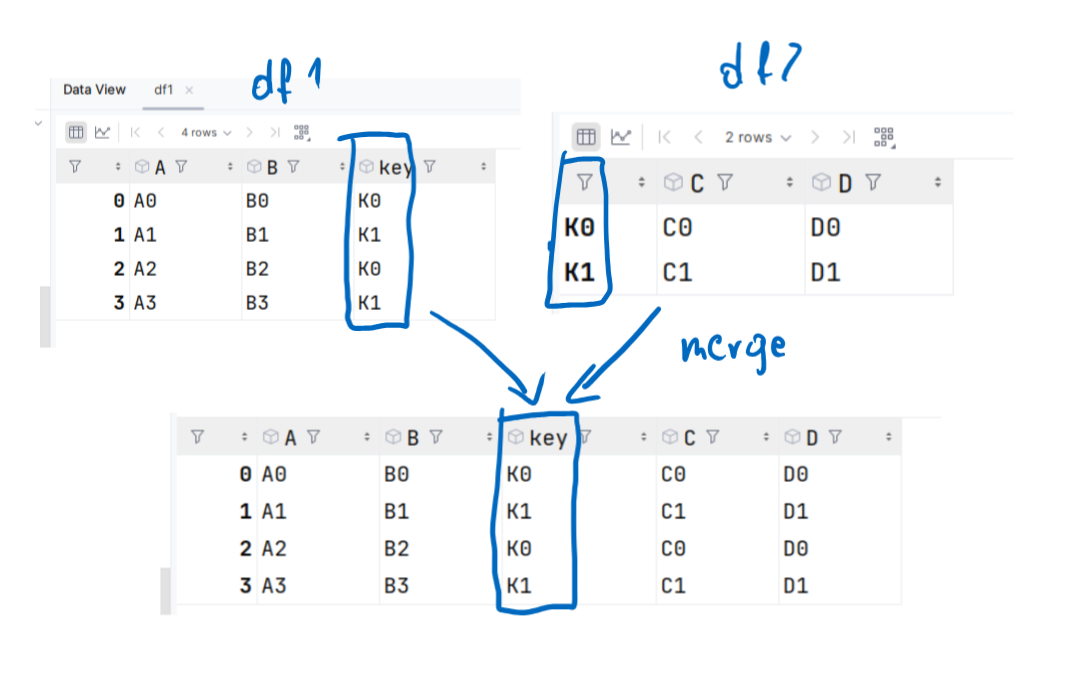
\includegraphics[keepaspectratio]{merge.png}}

\begin{Shaded}
\begin{Highlighting}[]
\ImportTok{import}\NormalTok{ pandas }\ImportTok{as}\NormalTok{ pd}

\NormalTok{df1 }\OperatorTok{=}\NormalTok{ pd.DataFrame(\{}
    \StringTok{\textquotesingle{}key\textquotesingle{}}\NormalTok{: [}\StringTok{\textquotesingle{}K0\textquotesingle{}}\NormalTok{, }\StringTok{\textquotesingle{}K1\textquotesingle{}}\NormalTok{, }\StringTok{\textquotesingle{}K2\textquotesingle{}}\NormalTok{, }\StringTok{\textquotesingle{}K3\textquotesingle{}}\NormalTok{],}
    \StringTok{\textquotesingle{}A\textquotesingle{}}\NormalTok{: [}\StringTok{\textquotesingle{}A0\textquotesingle{}}\NormalTok{, }\StringTok{\textquotesingle{}A1\textquotesingle{}}\NormalTok{, }\StringTok{\textquotesingle{}A2\textquotesingle{}}\NormalTok{, }\StringTok{\textquotesingle{}A3\textquotesingle{}}\NormalTok{],}
    \StringTok{\textquotesingle{}B\textquotesingle{}}\NormalTok{: [}\StringTok{\textquotesingle{}B0\textquotesingle{}}\NormalTok{, }\StringTok{\textquotesingle{}B1\textquotesingle{}}\NormalTok{, }\StringTok{\textquotesingle{}B2\textquotesingle{}}\NormalTok{, }\StringTok{\textquotesingle{}B3\textquotesingle{}}\NormalTok{]}
\NormalTok{\})}

\NormalTok{df2 }\OperatorTok{=}\NormalTok{ pd.DataFrame(\{}
    \StringTok{\textquotesingle{}key\textquotesingle{}}\NormalTok{: [}\StringTok{\textquotesingle{}K0\textquotesingle{}}\NormalTok{, }\StringTok{\textquotesingle{}K1\textquotesingle{}}\NormalTok{, }\StringTok{\textquotesingle{}K4\textquotesingle{}}\NormalTok{, }\StringTok{\textquotesingle{}K5\textquotesingle{}}\NormalTok{],}
    \StringTok{\textquotesingle{}C\textquotesingle{}}\NormalTok{: [}\StringTok{\textquotesingle{}C0\textquotesingle{}}\NormalTok{, }\StringTok{\textquotesingle{}C1\textquotesingle{}}\NormalTok{, }\StringTok{\textquotesingle{}C2\textquotesingle{}}\NormalTok{, }\StringTok{\textquotesingle{}C3\textquotesingle{}}\NormalTok{],}
    \StringTok{\textquotesingle{}D\textquotesingle{}}\NormalTok{: [}\StringTok{\textquotesingle{}D0\textquotesingle{}}\NormalTok{, }\StringTok{\textquotesingle{}D1\textquotesingle{}}\NormalTok{, }\StringTok{\textquotesingle{}D2\textquotesingle{}}\NormalTok{, }\StringTok{\textquotesingle{}D3\textquotesingle{}}\NormalTok{]}
\NormalTok{\})}

\BuiltInTok{print}\NormalTok{(df1)}

\BuiltInTok{print}\NormalTok{(df2)}

\NormalTok{inner\_merged\_df }\OperatorTok{=}\NormalTok{ df1.merge(df2, how}\OperatorTok{=}\StringTok{\textquotesingle{}inner\textquotesingle{}}\NormalTok{, on}\OperatorTok{=}\StringTok{\textquotesingle{}key\textquotesingle{}}\NormalTok{, suffixes}\OperatorTok{=}\NormalTok{(}\StringTok{\textquotesingle{}\_left\textquotesingle{}}\NormalTok{, }\StringTok{\textquotesingle{}\_right\textquotesingle{}}\NormalTok{),}
\NormalTok{                            indicator}\OperatorTok{=}\VariableTok{True}\NormalTok{)}
\NormalTok{outer\_merged\_df }\OperatorTok{=}\NormalTok{ df1.merge(df2, how}\OperatorTok{=}\StringTok{\textquotesingle{}outer\textquotesingle{}}\NormalTok{, on}\OperatorTok{=}\StringTok{\textquotesingle{}key\textquotesingle{}}\NormalTok{, suffixes}\OperatorTok{=}\NormalTok{(}\StringTok{\textquotesingle{}\_left\textquotesingle{}}\NormalTok{, }\StringTok{\textquotesingle{}\_right\textquotesingle{}}\NormalTok{),}
\NormalTok{                            indicator}\OperatorTok{=}\VariableTok{True}\NormalTok{)}
\NormalTok{left\_merged\_df }\OperatorTok{=}\NormalTok{ df1.merge(df2, how}\OperatorTok{=}\StringTok{\textquotesingle{}left\textquotesingle{}}\NormalTok{, on}\OperatorTok{=}\StringTok{\textquotesingle{}key\textquotesingle{}}\NormalTok{, suffixes}\OperatorTok{=}\NormalTok{(}\StringTok{\textquotesingle{}\_left\textquotesingle{}}\NormalTok{, }\StringTok{\textquotesingle{}\_right\textquotesingle{}}\NormalTok{),}
\NormalTok{                           indicator}\OperatorTok{=}\VariableTok{True}\NormalTok{)}
\NormalTok{right\_merged\_df }\OperatorTok{=}\NormalTok{ df1.merge(df2, how}\OperatorTok{=}\StringTok{\textquotesingle{}right\textquotesingle{}}\NormalTok{, on}\OperatorTok{=}\StringTok{\textquotesingle{}key\textquotesingle{}}\NormalTok{, suffixes}\OperatorTok{=}\NormalTok{(}\StringTok{\textquotesingle{}\_left\textquotesingle{}}\NormalTok{, }\StringTok{\textquotesingle{}\_right\textquotesingle{}}\NormalTok{),}
\NormalTok{                            indicator}\OperatorTok{=}\VariableTok{True}\NormalTok{)}

\BuiltInTok{print}\NormalTok{(}\StringTok{"Inner join"}\NormalTok{)}
\BuiltInTok{print}\NormalTok{(inner\_merged\_df)}

\BuiltInTok{print}\NormalTok{(}\StringTok{"Outer join"}\NormalTok{)}
\BuiltInTok{print}\NormalTok{(outer\_merged\_df)}

\BuiltInTok{print}\NormalTok{(}\StringTok{"Left join"}\NormalTok{)}
\BuiltInTok{print}\NormalTok{(left\_merged\_df)}

\BuiltInTok{print}\NormalTok{(}\StringTok{"Right join"}\NormalTok{)}
\BuiltInTok{print}\NormalTok{(right\_merged\_df)}
\end{Highlighting}
\end{Shaded}

\begin{verbatim}
  key   A   B
0  K0  A0  B0
1  K1  A1  B1
2  K2  A2  B2
3  K3  A3  B3
  key   C   D
0  K0  C0  D0
1  K1  C1  D1
2  K4  C2  D2
3  K5  C3  D3
Inner join
  key   A   B   C   D _merge
0  K0  A0  B0  C0  D0   both
1  K1  A1  B1  C1  D1   both
Outer join
  key    A    B    C    D      _merge
0  K0   A0   B0   C0   D0        both
1  K1   A1   B1   C1   D1        both
2  K2   A2   B2  NaN  NaN   left_only
3  K3   A3   B3  NaN  NaN   left_only
4  K4  NaN  NaN   C2   D2  right_only
5  K5  NaN  NaN   C3   D3  right_only
Left join
  key   A   B    C    D     _merge
0  K0  A0  B0   C0   D0       both
1  K1  A1  B1   C1   D1       both
2  K2  A2  B2  NaN  NaN  left_only
3  K3  A3  B3  NaN  NaN  left_only
Right join
  key    A    B   C   D      _merge
0  K0   A0   B0  C0  D0        both
1  K1   A1   B1  C1  D1        both
2  K4  NaN  NaN  C2  D2  right_only
3  K5  NaN  NaN  C3  D3  right_only
\end{verbatim}

\pandocbounded{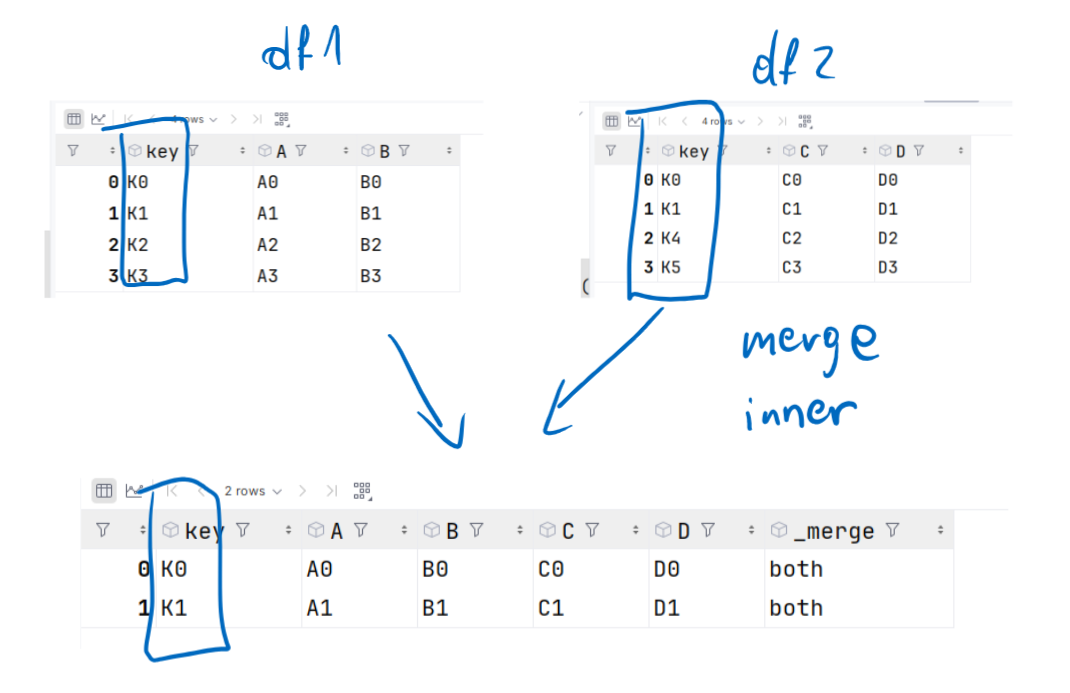
\includegraphics[keepaspectratio]{merge_inner.png}}

\pandocbounded{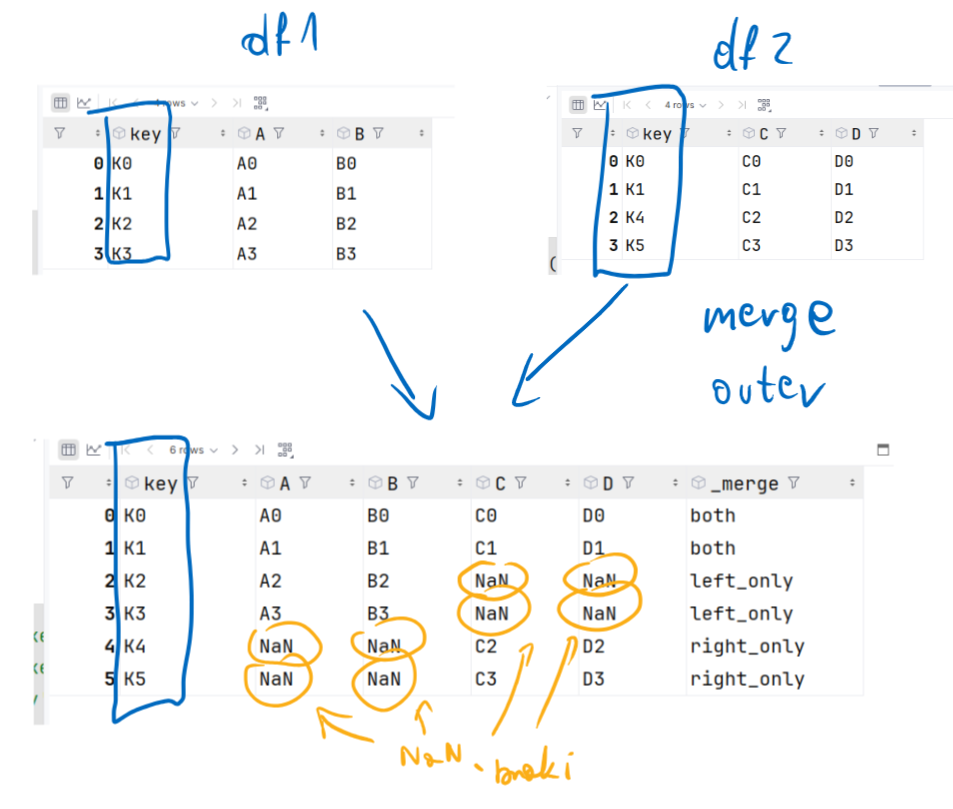
\includegraphics[keepaspectratio]{merge_outer.png}}

\pandocbounded{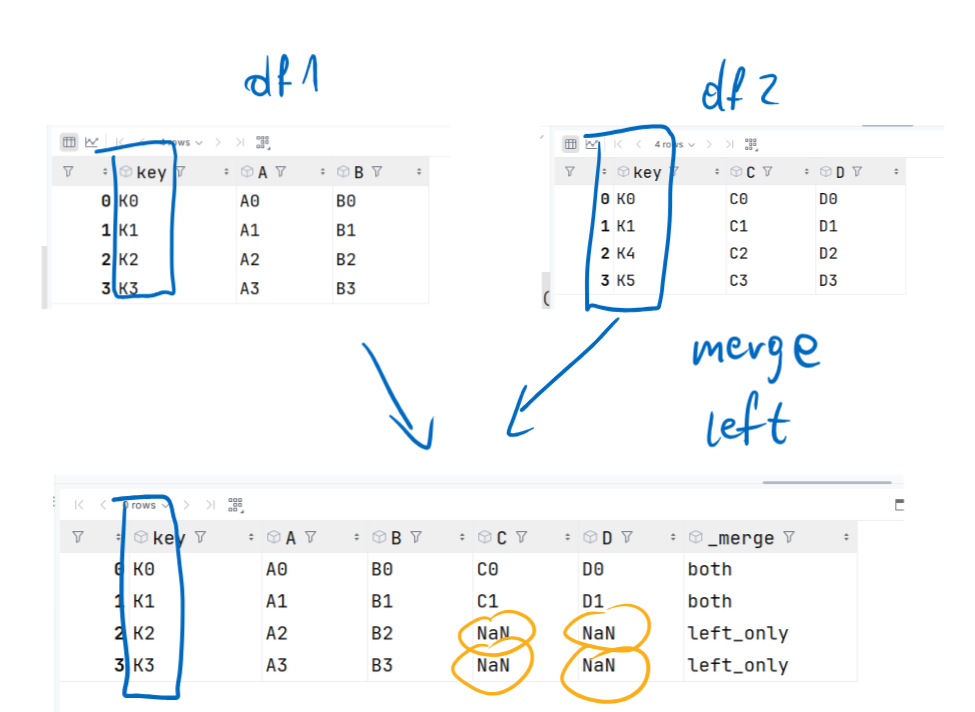
\includegraphics[keepaspectratio]{merge_left.png}}

\pandocbounded{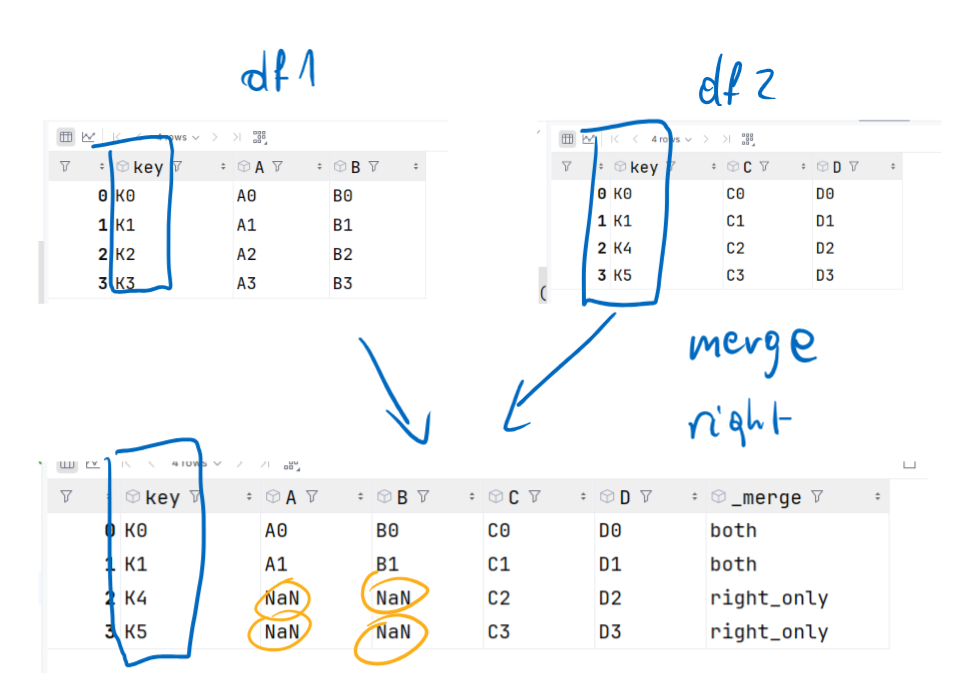
\includegraphics[keepaspectratio]{merge_right.png}}

\begin{itemize}
\tightlist
\item
  \texttt{join}
\end{itemize}

\url{https://pandas.pydata.org/docs/reference/api/pandas.DataFrame.join.html}

Metoda \texttt{join} jest używana do łączenia dwóch ramek danych wzdłuż
osi.

Podstawowe użycie tej metody wygląda następująco:

\begin{Shaded}
\begin{Highlighting}[]
\NormalTok{DataFrame.join(other, on}\OperatorTok{=}\VariableTok{None}\NormalTok{, how}\OperatorTok{=}\StringTok{\textquotesingle{}left\textquotesingle{}}\NormalTok{, lsuffix}\OperatorTok{=}\StringTok{\textquotesingle{}\textquotesingle{}}\NormalTok{, rsuffix}\OperatorTok{=}\StringTok{\textquotesingle{}\textquotesingle{}}\NormalTok{, sort}\OperatorTok{=}\VariableTok{False}\NormalTok{)}
\end{Highlighting}
\end{Shaded}

Gdzie:

\begin{itemize}
\tightlist
\item
  \texttt{other}: ramka danych, którą chcesz dołączyć do oryginalnej
  ramki danych.
\item
  \texttt{on}: nazwa lub lista nazw kolumn w oryginalnej ramxce danych,
  do których chcesz dołączyć.
\item
  \texttt{how}: określa typ łączenia. Dostępne są cztery typy: `inner',
  `outer', `left' i `right'. `left' to domyślna wartość, która zwraca
  wszystkie wiersze z oryginalnej ramki danych i pasujące wiersze z
  drugiej ramki danych. Wartości są uzupełniane wartością NaN, jeśli nie
  ma dopasowania.
\item
  \texttt{lsuffix} i \texttt{rsuffix}: sufiksy do dodania do kolumn,
  które się powtarzają. Domyślnie jest to puste.
\item
  \texttt{sort}: czy sortować dane według klucza.
\end{itemize}

\begin{Shaded}
\begin{Highlighting}[]
\ImportTok{import}\NormalTok{ pandas }\ImportTok{as}\NormalTok{ pd}

\NormalTok{df1 }\OperatorTok{=}\NormalTok{ pd.DataFrame(\{}
    \StringTok{\textquotesingle{}A\textquotesingle{}}\NormalTok{: [}\StringTok{\textquotesingle{}A0\textquotesingle{}}\NormalTok{, }\StringTok{\textquotesingle{}A1\textquotesingle{}}\NormalTok{, }\StringTok{\textquotesingle{}A2\textquotesingle{}}\NormalTok{],}
    \StringTok{\textquotesingle{}B\textquotesingle{}}\NormalTok{: [}\StringTok{\textquotesingle{}B0\textquotesingle{}}\NormalTok{, }\StringTok{\textquotesingle{}B1\textquotesingle{}}\NormalTok{, }\StringTok{\textquotesingle{}B2\textquotesingle{}}\NormalTok{]\},}
\NormalTok{    index}\OperatorTok{=}\NormalTok{[}\StringTok{\textquotesingle{}K0\textquotesingle{}}\NormalTok{, }\StringTok{\textquotesingle{}K1\textquotesingle{}}\NormalTok{, }\StringTok{\textquotesingle{}K2\textquotesingle{}}\NormalTok{]}
\NormalTok{)}

\NormalTok{df2 }\OperatorTok{=}\NormalTok{ pd.DataFrame(\{}
    \StringTok{\textquotesingle{}C\textquotesingle{}}\NormalTok{: [}\StringTok{\textquotesingle{}C0\textquotesingle{}}\NormalTok{, }\StringTok{\textquotesingle{}C2\textquotesingle{}}\NormalTok{, }\StringTok{\textquotesingle{}C3\textquotesingle{}}\NormalTok{],}
    \StringTok{\textquotesingle{}D\textquotesingle{}}\NormalTok{: [}\StringTok{\textquotesingle{}D0\textquotesingle{}}\NormalTok{, }\StringTok{\textquotesingle{}D2\textquotesingle{}}\NormalTok{, }\StringTok{\textquotesingle{}D3\textquotesingle{}}\NormalTok{]\},}
\NormalTok{    index}\OperatorTok{=}\NormalTok{[}\StringTok{\textquotesingle{}K0\textquotesingle{}}\NormalTok{, }\StringTok{\textquotesingle{}K2\textquotesingle{}}\NormalTok{, }\StringTok{\textquotesingle{}K3\textquotesingle{}}\NormalTok{]}
\NormalTok{)}

\BuiltInTok{print}\NormalTok{(df1)}

\BuiltInTok{print}\NormalTok{(df2)}

\NormalTok{joined\_df }\OperatorTok{=}\NormalTok{ df1.join(df2)}
\BuiltInTok{print}\NormalTok{(joined\_df)}
\end{Highlighting}
\end{Shaded}

\begin{verbatim}
     A   B
K0  A0  B0
K1  A1  B1
K2  A2  B2
     C   D
K0  C0  D0
K2  C2  D2
K3  C3  D3
     A   B    C    D
K0  A0  B0   C0   D0
K1  A1  B1  NaN  NaN
K2  A2  B2   C2   D2
\end{verbatim}

\pandocbounded{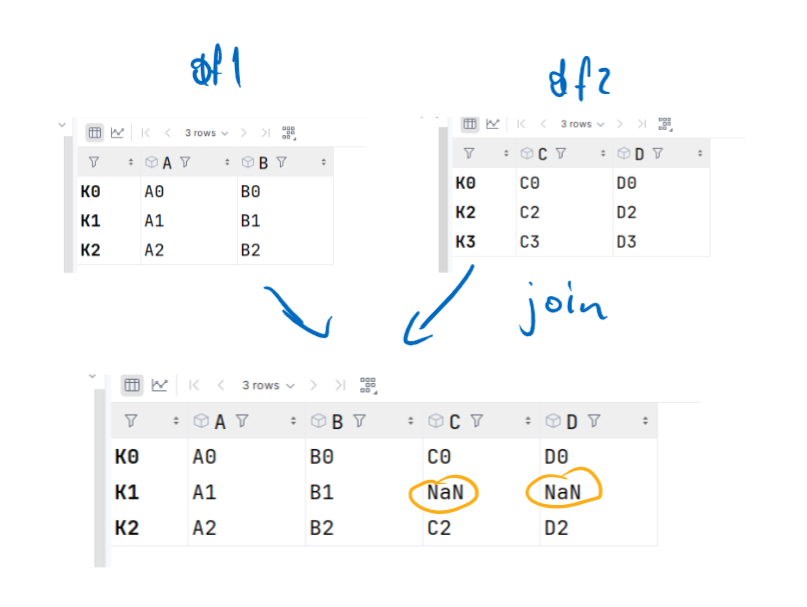
\includegraphics[keepaspectratio]{join.png}}

\begin{itemize}
\tightlist
\item
  \texttt{concat}
\end{itemize}

\url{https://pandas.pydata.org/docs/reference/api/pandas.concat.html}

Metoda \texttt{concat} jest używana do łączenia dwóch lub więcej ramek
danych wzdłuż określonej osi.

Podstawowe użycie tej metody wygląda następująco:

\begin{Shaded}
\begin{Highlighting}[]
\NormalTok{pandas.concat(objs, axis}\OperatorTok{=}\DecValTok{0}\NormalTok{, join}\OperatorTok{=}\StringTok{\textquotesingle{}outer\textquotesingle{}}\NormalTok{, ignore\_index}\OperatorTok{=}\VariableTok{False}\NormalTok{, keys}\OperatorTok{=}\VariableTok{None}\NormalTok{,}
\NormalTok{              levels}\OperatorTok{=}\VariableTok{None}\NormalTok{, names}\OperatorTok{=}\VariableTok{None}\NormalTok{, verify\_integrity}\OperatorTok{=}\VariableTok{False}\NormalTok{, sort}\OperatorTok{=}\VariableTok{False}\NormalTok{,}
\NormalTok{              copy}\OperatorTok{=}\VariableTok{True}\NormalTok{)}
\end{Highlighting}
\end{Shaded}

Gdzie:

\begin{itemize}
\tightlist
\item
  \texttt{objs}: sekwencja ramek danych, które chcesz połączyć.
\item
  \texttt{axis}: oś, wzdłuż której chcesz łączyć ramki danych. Domyślnie
  to 0 (łączenie wierszy, pionowo), ale można także ustawić na 1
  (łączenie kolumn, poziomo).
\item
  \texttt{join}: określa typ łączenia. Dostępne są dwa typy: `outer' i
  `inner'. `outer' to domyślna wartość, która zwraca wszystkie kolumny z
  każdej ramki danych. `inner' zwraca tylko te kolumny, które są wspólne
  dla wszystkich ramek danych.
\item
  \texttt{ignore\_index}: jeśli ustawione na True, nie używa indeksów z
  ramek danych do tworzenia indeksu w wynikowej ramce danych. Zamiast
  tego tworzy nowy indeks od 0 do n-1.
\item
  \texttt{keys}: wartości do skojarzenia z obiektami.
\item
  \texttt{levels}: określone indeksy dla nowej ramki danych.
\item
  \texttt{names}: nazwy dla poziomów indeksów (jeśli są wielopoziomowe).
\item
  \texttt{verify\_integrity}: sprawdza, czy nowy, skonkatenowana ramka
  danych nie ma powtarzających się indeksów.
\item
  \texttt{sort}: czy sortować niekonkatenacyjną oś (np. indeksy, jeśli
  axis=0), niezależnie od danych.
\item
  \texttt{copy}: czy zawsze kopiować dane, nawet jeśli nie są potrzebne.
\end{itemize}

\begin{Shaded}
\begin{Highlighting}[]
\ImportTok{import}\NormalTok{ pandas }\ImportTok{as}\NormalTok{ pd}

\NormalTok{df1 }\OperatorTok{=}\NormalTok{ pd.DataFrame(\{}
    \StringTok{\textquotesingle{}A\textquotesingle{}}\NormalTok{: [}\StringTok{\textquotesingle{}A0\textquotesingle{}}\NormalTok{, }\StringTok{\textquotesingle{}A1\textquotesingle{}}\NormalTok{, }\StringTok{\textquotesingle{}A2\textquotesingle{}}\NormalTok{],}
    \StringTok{\textquotesingle{}B\textquotesingle{}}\NormalTok{: [}\StringTok{\textquotesingle{}B0\textquotesingle{}}\NormalTok{, }\StringTok{\textquotesingle{}B1\textquotesingle{}}\NormalTok{, }\StringTok{\textquotesingle{}B2\textquotesingle{}}\NormalTok{]}
\NormalTok{\})}

\NormalTok{df2 }\OperatorTok{=}\NormalTok{ pd.DataFrame(\{}
    \StringTok{\textquotesingle{}A\textquotesingle{}}\NormalTok{: [}\StringTok{\textquotesingle{}A3\textquotesingle{}}\NormalTok{, }\StringTok{\textquotesingle{}A4\textquotesingle{}}\NormalTok{, }\StringTok{\textquotesingle{}A5\textquotesingle{}}\NormalTok{],}
    \StringTok{\textquotesingle{}B\textquotesingle{}}\NormalTok{: [}\StringTok{\textquotesingle{}B3\textquotesingle{}}\NormalTok{, }\StringTok{\textquotesingle{}B4\textquotesingle{}}\NormalTok{, }\StringTok{\textquotesingle{}B5\textquotesingle{}}\NormalTok{]}
\NormalTok{\})}

\BuiltInTok{print}\NormalTok{(df1)}

\BuiltInTok{print}\NormalTok{(df2)}

\NormalTok{concatenated\_df }\OperatorTok{=}\NormalTok{ pd.concat([df1, df2], ignore\_index}\OperatorTok{=}\VariableTok{True}\NormalTok{)}
\BuiltInTok{print}\NormalTok{(concatenated\_df)}
\end{Highlighting}
\end{Shaded}

\begin{verbatim}
    A   B
0  A0  B0
1  A1  B1
2  A2  B2
    A   B
0  A3  B3
1  A4  B4
2  A5  B5
    A   B
0  A0  B0
1  A1  B1
2  A2  B2
3  A3  B3
4  A4  B4
5  A5  B5
\end{verbatim}

\pandocbounded{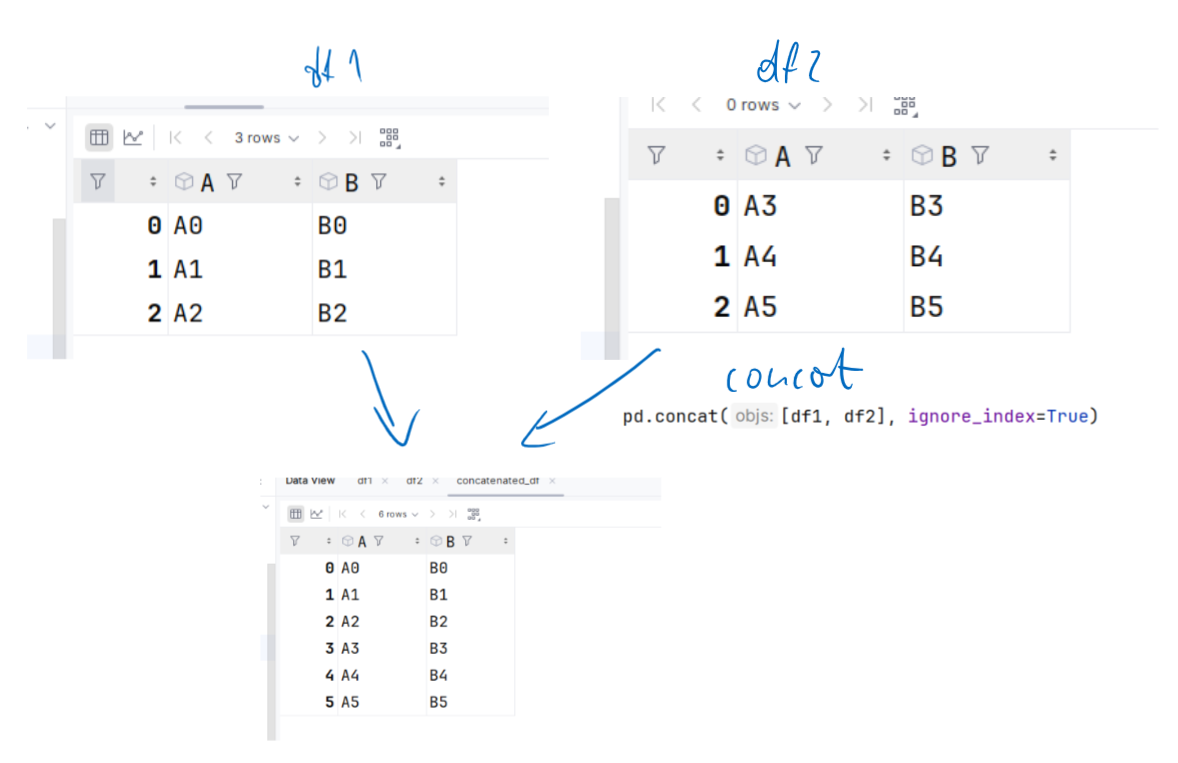
\includegraphics[keepaspectratio]{concat1.png}}

\begin{Shaded}
\begin{Highlighting}[]
\ImportTok{import}\NormalTok{ pandas }\ImportTok{as}\NormalTok{ pd}

\NormalTok{df1 }\OperatorTok{=}\NormalTok{ pd.DataFrame(\{}
    \StringTok{\textquotesingle{}A\textquotesingle{}}\NormalTok{: [}\StringTok{\textquotesingle{}A0\textquotesingle{}}\NormalTok{, }\StringTok{\textquotesingle{}A1\textquotesingle{}}\NormalTok{, }\StringTok{\textquotesingle{}A2\textquotesingle{}}\NormalTok{],}
    \StringTok{\textquotesingle{}B\textquotesingle{}}\NormalTok{: [}\StringTok{\textquotesingle{}B0\textquotesingle{}}\NormalTok{, }\StringTok{\textquotesingle{}B1\textquotesingle{}}\NormalTok{, }\StringTok{\textquotesingle{}B2\textquotesingle{}}\NormalTok{]}
\NormalTok{\})}

\NormalTok{df2 }\OperatorTok{=}\NormalTok{ pd.DataFrame(\{}
    \StringTok{\textquotesingle{}C\textquotesingle{}}\NormalTok{: [}\StringTok{\textquotesingle{}C0\textquotesingle{}}\NormalTok{, }\StringTok{\textquotesingle{}C1\textquotesingle{}}\NormalTok{, }\StringTok{\textquotesingle{}C2\textquotesingle{}}\NormalTok{],}
    \StringTok{\textquotesingle{}D\textquotesingle{}}\NormalTok{: [}\StringTok{\textquotesingle{}D0\textquotesingle{}}\NormalTok{, }\StringTok{\textquotesingle{}D1\textquotesingle{}}\NormalTok{, }\StringTok{\textquotesingle{}D2\textquotesingle{}}\NormalTok{]}
\NormalTok{\})}

\BuiltInTok{print}\NormalTok{(df1)}

\BuiltInTok{print}\NormalTok{(df2)}

\NormalTok{concatenated\_df\_axis1 }\OperatorTok{=}\NormalTok{ pd.concat([df1, df2], axis}\OperatorTok{=}\DecValTok{1}\NormalTok{)}
\NormalTok{concatenated\_df\_keys }\OperatorTok{=}\NormalTok{ pd.concat([df1, df2], keys}\OperatorTok{=}\NormalTok{[}\StringTok{\textquotesingle{}df1\textquotesingle{}}\NormalTok{, }\StringTok{\textquotesingle{}df2\textquotesingle{}}\NormalTok{])}

\BuiltInTok{print}\NormalTok{(concatenated\_df\_axis1)}
\BuiltInTok{print}\NormalTok{(concatenated\_df\_keys)}
\end{Highlighting}
\end{Shaded}

\begin{verbatim}
    A   B
0  A0  B0
1  A1  B1
2  A2  B2
    C   D
0  C0  D0
1  C1  D1
2  C2  D2
    A   B   C   D
0  A0  B0  C0  D0
1  A1  B1  C1  D1
2  A2  B2  C2  D2
         A    B    C    D
df1 0   A0   B0  NaN  NaN
    1   A1   B1  NaN  NaN
    2   A2   B2  NaN  NaN
df2 0  NaN  NaN   C0   D0
    1  NaN  NaN   C1   D1
    2  NaN  NaN   C2   D2
\end{verbatim}

\pandocbounded{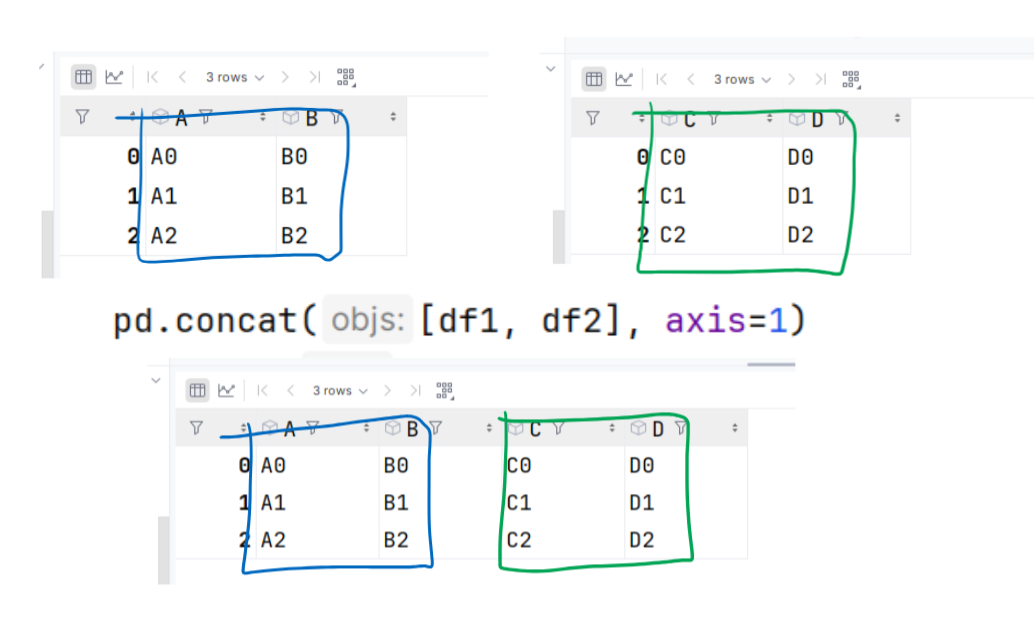
\includegraphics[keepaspectratio]{concat2.png}}

\pandocbounded{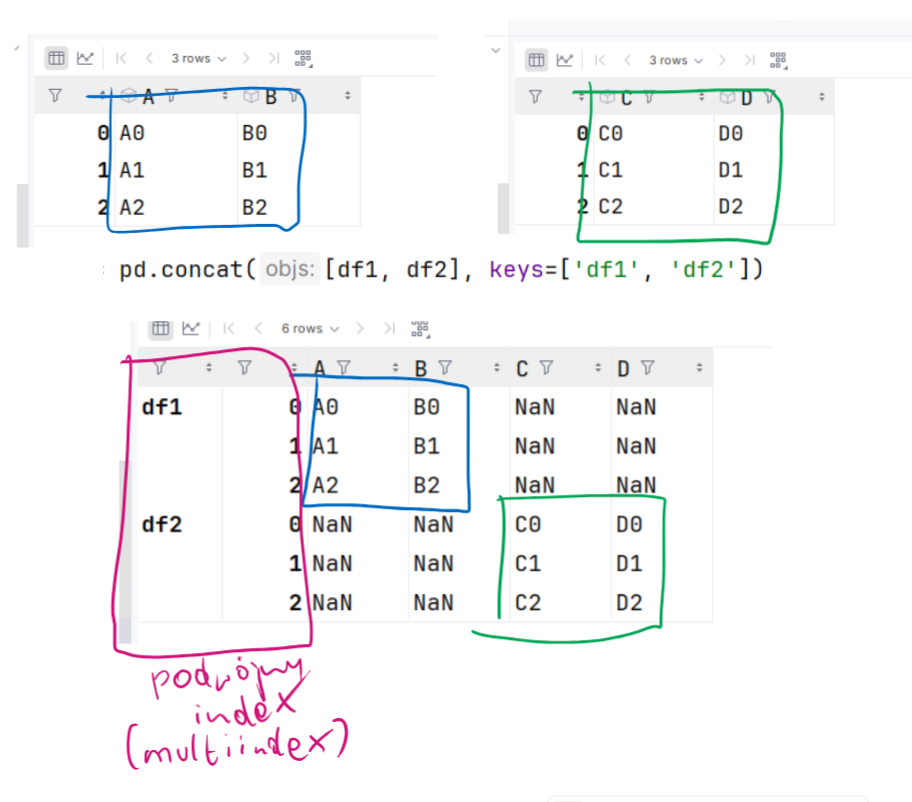
\includegraphics[keepaspectratio]{concat3.png}}

\begin{itemize}
\tightlist
\item
  \texttt{pivot}
\end{itemize}

\url{https://pandas.pydata.org/docs/reference/api/pandas.DataFrame.pivot.html}

\pandocbounded{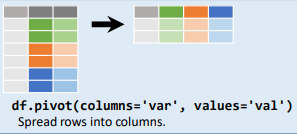
\includegraphics[keepaspectratio]{62.png}}

Metoda \texttt{pivot} jest używana do przekształcenia danych z formatu
``długiego'' do ``szerokiego''.

Podstawowe użycie tej metody wygląda następująco:

\begin{Shaded}
\begin{Highlighting}[]
\NormalTok{DataFrame.pivot(index}\OperatorTok{=}\VariableTok{None}\NormalTok{, columns}\OperatorTok{=}\VariableTok{None}\NormalTok{, values}\OperatorTok{=}\VariableTok{None}\NormalTok{)}
\end{Highlighting}
\end{Shaded}

Gdzie:

\begin{itemize}
\tightlist
\item
  \texttt{index}: nazwa kolumny lub lista nazw kolumn, które mają stać
  się indeksem w nowej ramce danych.
\item
  \texttt{columns}: nazwa kolumny, z której unikalne wartości mają stać
  się kolumnami w nowej ramce danych.
\item
  \texttt{values}: nazwa kolumny lub lista nazw kolumn, które mają stać
  się wartościami dla nowych kolumn w nowej ramce danych.
\end{itemize}

\begin{Shaded}
\begin{Highlighting}[]
\ImportTok{import}\NormalTok{ pandas }\ImportTok{as}\NormalTok{ pd}

\NormalTok{df }\OperatorTok{=}\NormalTok{ pd.DataFrame(\{}
    \StringTok{\textquotesingle{}foo\textquotesingle{}}\NormalTok{: [}\StringTok{\textquotesingle{}one\textquotesingle{}}\NormalTok{, }\StringTok{\textquotesingle{}one\textquotesingle{}}\NormalTok{, }\StringTok{\textquotesingle{}one\textquotesingle{}}\NormalTok{, }\StringTok{\textquotesingle{}two\textquotesingle{}}\NormalTok{, }\StringTok{\textquotesingle{}two\textquotesingle{}}\NormalTok{, }\StringTok{\textquotesingle{}two\textquotesingle{}}\NormalTok{],}
    \StringTok{\textquotesingle{}bar\textquotesingle{}}\NormalTok{: [}\StringTok{\textquotesingle{}A\textquotesingle{}}\NormalTok{, }\StringTok{\textquotesingle{}B\textquotesingle{}}\NormalTok{, }\StringTok{\textquotesingle{}C\textquotesingle{}}\NormalTok{, }\StringTok{\textquotesingle{}A\textquotesingle{}}\NormalTok{, }\StringTok{\textquotesingle{}B\textquotesingle{}}\NormalTok{, }\StringTok{\textquotesingle{}C\textquotesingle{}}\NormalTok{],}
    \StringTok{\textquotesingle{}baz\textquotesingle{}}\NormalTok{: [}\DecValTok{1}\NormalTok{, }\DecValTok{2}\NormalTok{, }\DecValTok{3}\NormalTok{, }\DecValTok{4}\NormalTok{, }\DecValTok{5}\NormalTok{, }\DecValTok{6}\NormalTok{],}
    \StringTok{\textquotesingle{}zoo\textquotesingle{}}\NormalTok{: [}\StringTok{\textquotesingle{}x\textquotesingle{}}\NormalTok{, }\StringTok{\textquotesingle{}y\textquotesingle{}}\NormalTok{, }\StringTok{\textquotesingle{}z\textquotesingle{}}\NormalTok{, }\StringTok{\textquotesingle{}q\textquotesingle{}}\NormalTok{, }\StringTok{\textquotesingle{}w\textquotesingle{}}\NormalTok{, }\StringTok{\textquotesingle{}t\textquotesingle{}}\NormalTok{],}
\NormalTok{\})}

\BuiltInTok{print}\NormalTok{(df)}

\NormalTok{pivot\_df }\OperatorTok{=}\NormalTok{ df.pivot(index}\OperatorTok{=}\StringTok{\textquotesingle{}foo\textquotesingle{}}\NormalTok{, columns}\OperatorTok{=}\StringTok{\textquotesingle{}bar\textquotesingle{}}\NormalTok{, values}\OperatorTok{=}\StringTok{\textquotesingle{}baz\textquotesingle{}}\NormalTok{)}
\BuiltInTok{print}\NormalTok{(pivot\_df)}
\end{Highlighting}
\end{Shaded}

\begin{verbatim}
   foo bar  baz zoo
0  one   A    1   x
1  one   B    2   y
2  one   C    3   z
3  two   A    4   q
4  two   B    5   w
5  two   C    6   t
bar  A  B  C
foo         
one  1  2  3
two  4  5  6
\end{verbatim}

\pandocbounded{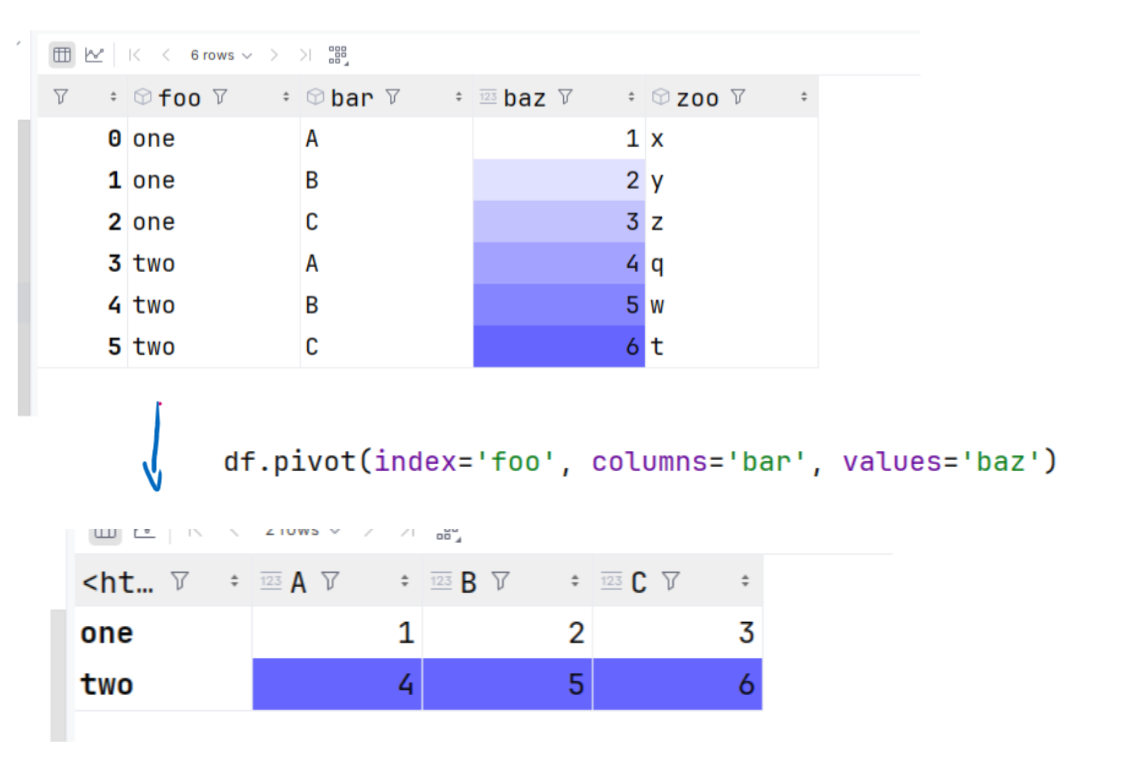
\includegraphics[keepaspectratio]{pivot.png}}

\begin{itemize}
\tightlist
\item
  \texttt{wide\_to\_long}
\end{itemize}

\url{https://pandas.pydata.org/docs/reference/api/pandas.wide_to_long.html}

Metoda \texttt{wide\_to\_long} jest używana do przekształcenia danych z
szerokiego formatu (gdzie każda kolumna zawiera wiele zmiennych) do
długiego formatu (gdzie każda kolumna zawiera jedną zmienną z wieloma
pomiarami). Jest to przydatne, gdy mamy dane, które są rozłożone w wielu
kolumnach z powtarzającymi się lub sekwencyjnymi nazwami, i chcemy
przekształcić te dane w sposób, który ułatwia analizę i wizualizację.

Wyjaśnienie parametrów \texttt{wide\_to\_long}

\begin{itemize}
\tightlist
\item
  \textbf{stubnames}: Lista początkowych części nazw kolumn, które mają
  zostać przekształcone.
\item
  \textbf{i}: Nazwa kolumny lub lista kolumn, które identyfikują
  poszczególne wiersze. W naszym przykładzie jest to \texttt{id}, które
  unikalnie identyfikuje osobę.
\item
  \textbf{j}: Nazwa nowej kolumny, w której będą przechowywane różne
  poziomy zmiennych (w naszym przypadku rok).
\item
  \textbf{sep}: Opcjonalny separator (domyślnie \texttt{""}).
\end{itemize}

\begin{Shaded}
\begin{Highlighting}[]
\ImportTok{import}\NormalTok{ pandas }\ImportTok{as}\NormalTok{ pd}

\CommentTok{\# Przykładowe dane}
\NormalTok{data }\OperatorTok{=}\NormalTok{ \{}
    \StringTok{\textquotesingle{}id\textquotesingle{}}\NormalTok{: [}\StringTok{\textquotesingle{}A\textquotesingle{}}\NormalTok{, }\StringTok{\textquotesingle{}B\textquotesingle{}}\NormalTok{, }\StringTok{\textquotesingle{}C\textquotesingle{}}\NormalTok{],}
    \StringTok{\textquotesingle{}height\_2020\textquotesingle{}}\NormalTok{: [}\DecValTok{180}\NormalTok{, }\DecValTok{175}\NormalTok{, }\DecValTok{165}\NormalTok{],}
    \StringTok{\textquotesingle{}weight\_2020\textquotesingle{}}\NormalTok{: [}\DecValTok{70}\NormalTok{, }\DecValTok{76}\NormalTok{, }\DecValTok{65}\NormalTok{],}
    \StringTok{\textquotesingle{}height\_2021\textquotesingle{}}\NormalTok{: [}\DecValTok{181}\NormalTok{, }\DecValTok{176}\NormalTok{, }\DecValTok{166}\NormalTok{],}
    \StringTok{\textquotesingle{}weight\_2021\textquotesingle{}}\NormalTok{: [}\DecValTok{71}\NormalTok{, }\DecValTok{77}\NormalTok{, }\DecValTok{66}\NormalTok{]}
\NormalTok{\}}

\NormalTok{data2 }\OperatorTok{=}\NormalTok{ pd.DataFrame(data)}

\CommentTok{\# Przekształcenie do formatu długiego}
\NormalTok{df\_long }\OperatorTok{=}\NormalTok{ pd.wide\_to\_long(data2, stubnames}\OperatorTok{=}\NormalTok{[}\StringTok{\textquotesingle{}height\textquotesingle{}}\NormalTok{, }\StringTok{\textquotesingle{}weight\textquotesingle{}}\NormalTok{], i}\OperatorTok{=}\StringTok{\textquotesingle{}id\textquotesingle{}}\NormalTok{, j}\OperatorTok{=}\StringTok{\textquotesingle{}year\textquotesingle{}}\NormalTok{, sep}\OperatorTok{=}\StringTok{\textquotesingle{}\_\textquotesingle{}}\NormalTok{)}
\NormalTok{df\_long }\OperatorTok{=}\NormalTok{ df\_long.reset\_index()}

\BuiltInTok{print}\NormalTok{(df\_long)}
\end{Highlighting}
\end{Shaded}

\begin{verbatim}
  id  year  height  weight
0  A  2020     180      70
1  B  2020     175      76
2  C  2020     165      65
3  A  2021     181      71
4  B  2021     176      77
5  C  2021     166      66
\end{verbatim}

\pandocbounded{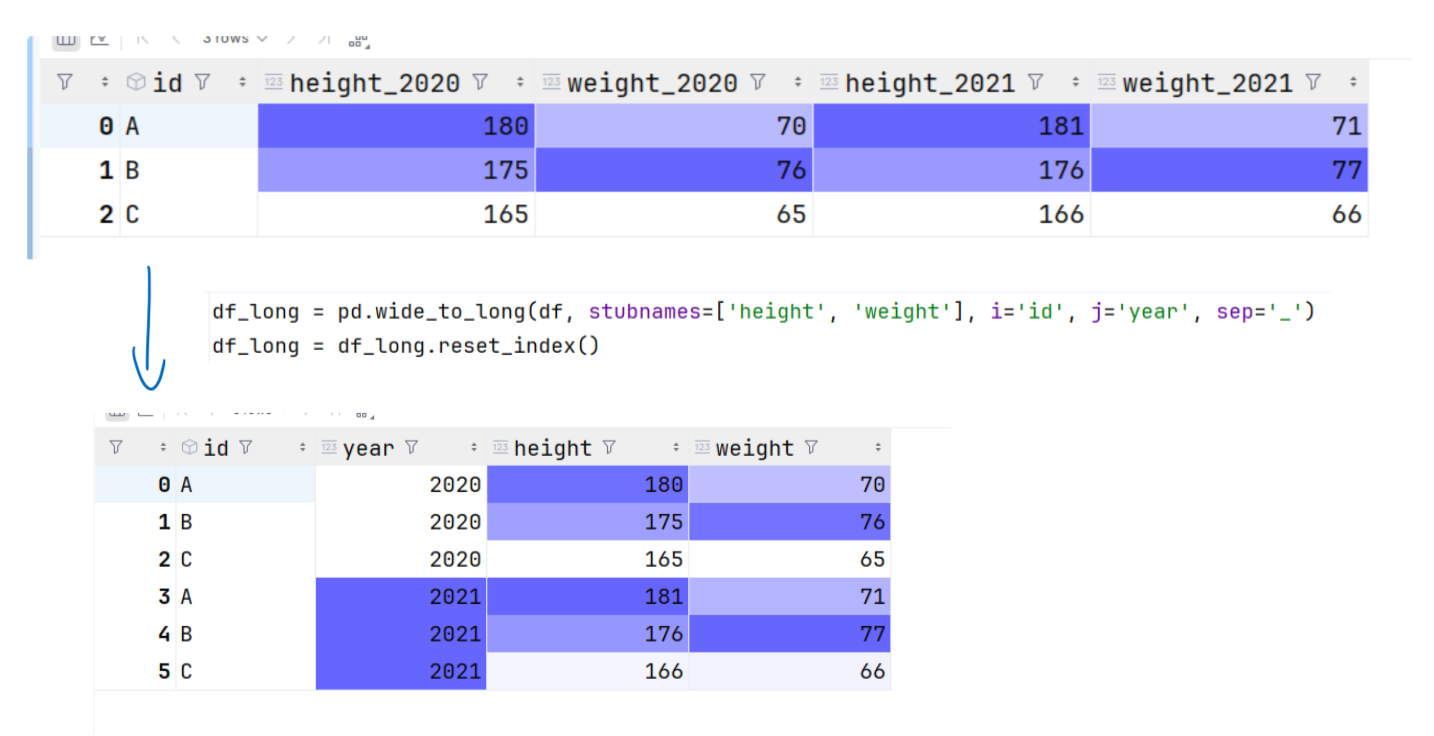
\includegraphics[keepaspectratio]{wide_to_long.png}}

\begin{itemize}
\tightlist
\item
  \texttt{melt}
\end{itemize}

\pandocbounded{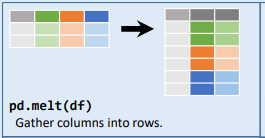
\includegraphics[keepaspectratio]{61.png}}

\url{https://pandas.pydata.org/docs/reference/api/pandas.DataFrame.melt.html}

Funkcja \texttt{melt} służy do przekształcania danych z formatu
szerokiego na długi.

Podstawowe użycie tej metody wygląda następująco:

\begin{Shaded}
\begin{Highlighting}[]
\NormalTok{pandas.melt(frame, id\_vars}\OperatorTok{=}\VariableTok{None}\NormalTok{, value\_vars}\OperatorTok{=}\VariableTok{None}\NormalTok{, var\_name}\OperatorTok{=}\VariableTok{None}\NormalTok{, value\_name}\OperatorTok{=}\StringTok{\textquotesingle{}value\textquotesingle{}}\NormalTok{, col\_level}\OperatorTok{=}\VariableTok{None}\NormalTok{)}
\end{Highlighting}
\end{Shaded}

Gdzie:

\begin{itemize}
\tightlist
\item
  \texttt{frame}: ramka danych, którą chcesz przetworzyć.
\item
  \texttt{id\_vars}: kolumna(y), które chcesz zachować jako
  identyfikatory. Te kolumny nie będą zmieniane.
\item
  \texttt{value\_vars}: kolumna(y), które chcesz przekształcić na pary
  klucz-wartość. Jeżeli nie jest podane, wszystkie kolumny nie będące
  \texttt{id\_vars} zostaną użyte.
\item
  \texttt{var\_name}: nazwa nowej kolumny, która będzie zawierała nazwy
  kolumn przekształconych na pary klucz-wartość. Domyślnie to
  `variable'.
\item
  \texttt{value\_name}: nazwa nowej kolumny, która będzie zawierała
  wartości kolumn przekształconych na pary klucz-wartość. Domyślnie to
  `value'.
\item
  \texttt{col\_level}: jeżeli kolumny są wielopoziomowe, to jest poziom,
  który będzie użyty do przekształcania kolumn na pary klucz-wartość.
\end{itemize}

\begin{Shaded}
\begin{Highlighting}[]
\ImportTok{import}\NormalTok{ pandas }\ImportTok{as}\NormalTok{ pd}

\NormalTok{data }\OperatorTok{=}\NormalTok{ pd.DataFrame(\{}
    \StringTok{\textquotesingle{}A\textquotesingle{}}\NormalTok{: [}\StringTok{\textquotesingle{}foo\textquotesingle{}}\NormalTok{, }\StringTok{\textquotesingle{}bar\textquotesingle{}}\NormalTok{, }\StringTok{\textquotesingle{}baz\textquotesingle{}}\NormalTok{],}
    \StringTok{\textquotesingle{}B\textquotesingle{}}\NormalTok{: [}\StringTok{\textquotesingle{}one\textquotesingle{}}\NormalTok{, }\StringTok{\textquotesingle{}one\textquotesingle{}}\NormalTok{, }\StringTok{\textquotesingle{}two\textquotesingle{}}\NormalTok{],}
    \StringTok{\textquotesingle{}C\textquotesingle{}}\NormalTok{: [}\FloatTok{2.0}\NormalTok{, }\FloatTok{1.0}\NormalTok{, }\FloatTok{3.0}\NormalTok{],}
    \StringTok{\textquotesingle{}D\textquotesingle{}}\NormalTok{: [}\FloatTok{3.0}\NormalTok{, }\FloatTok{2.0}\NormalTok{, }\FloatTok{1.0}\NormalTok{]}
\NormalTok{\})}
\BuiltInTok{print}\NormalTok{(data)}
\NormalTok{melted\_df }\OperatorTok{=}\NormalTok{ data.melt(id\_vars}\OperatorTok{=}\NormalTok{[}\StringTok{\textquotesingle{}A\textquotesingle{}}\NormalTok{, }\StringTok{\textquotesingle{}B\textquotesingle{}}\NormalTok{], value\_vars}\OperatorTok{=}\NormalTok{[}\StringTok{\textquotesingle{}C\textquotesingle{}}\NormalTok{, }\StringTok{\textquotesingle{}D\textquotesingle{}}\NormalTok{], var\_name}\OperatorTok{=}\StringTok{\textquotesingle{}My\_Var\textquotesingle{}}\NormalTok{,}
\NormalTok{                      value\_name}\OperatorTok{=}\StringTok{\textquotesingle{}My\_Val\textquotesingle{}}\NormalTok{)}
\BuiltInTok{print}\NormalTok{(melted\_df)}
\end{Highlighting}
\end{Shaded}

\begin{verbatim}
     A    B    C    D
0  foo  one  2.0  3.0
1  bar  one  1.0  2.0
2  baz  two  3.0  1.0
     A    B My_Var  My_Val
0  foo  one      C     2.0
1  bar  one      C     1.0
2  baz  two      C     3.0
3  foo  one      D     3.0
4  bar  one      D     2.0
5  baz  two      D     1.0
\end{verbatim}

\pandocbounded{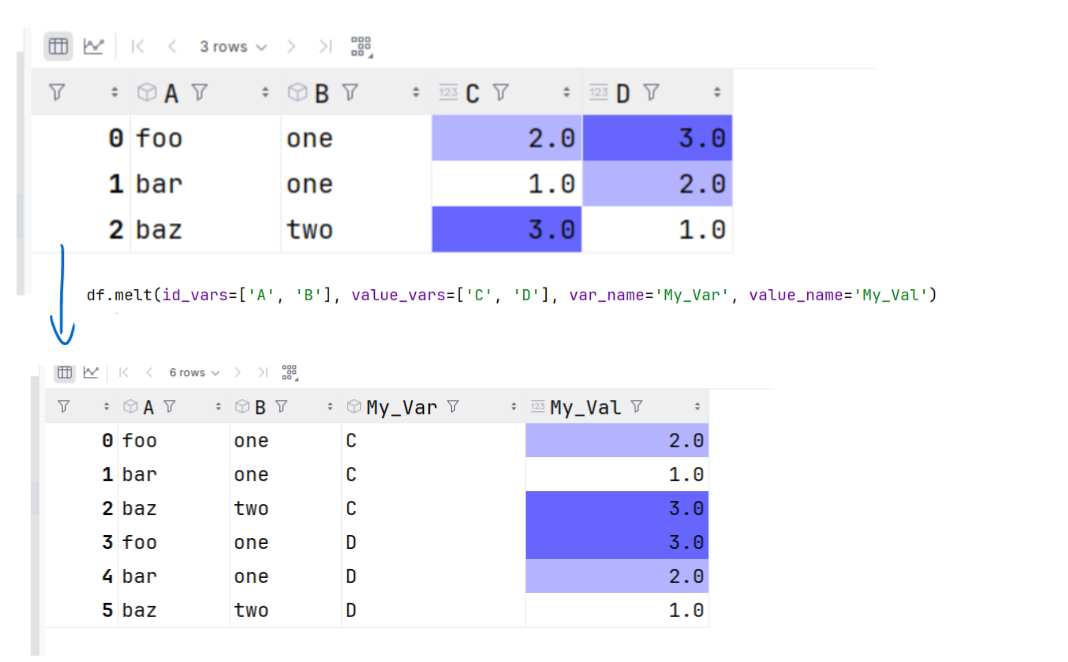
\includegraphics[keepaspectratio]{melt.png}}

\part{Analia struktury danych}

\chapter{Analiza struktury}\label{analiza-struktury}

Miary statystyczne

\begin{itemize}
\tightlist
\item
  to charakterystyki liczbowe pozwalające opisać właściwości rozkładu
  badanej cechy.
\item
  inne nazwy:

  \begin{itemize}
  \tightlist
  \item
    parametry - dane analizowane z całej populacji,
  \item
    statystyki próby - dane analizowane z próby.
  \end{itemize}
\end{itemize}

\textbf{Klasyfikacja miar statystycznych:}

\begin{itemize}
\tightlist
\item
  miary położenia (miary poziomu, miary przeciętne) - pozwalają określić
  gdzie w zbiorze wartości znajdują się dane pochodzące z obserwacji,
\item
  miary zróżnicowania (miary rozproszenia, zmienności, rozrzutu,
  dyspersji) - pozwalają określić zróżnicowanie jednostek,
\item
  miary asymetrii (miary skośności) - pozwalają określić asymetrię (czy
  większość jednostek ma wartości większe lub mniejsze względem
  przeciętnego poziomu),
\item
  miary koncentracji - pozwalają określić skupienie wartości względem
  średniej.
\end{itemize}

\section{Miary położenia}\label{miary-poux142oux17cenia}

\begin{itemize}
\tightlist
\item
  średnie klasyczne:

  \begin{itemize}
  \tightlist
  \item
    średnia arytmetyczna,
  \end{itemize}
\item
  średnie pozycyjne i kwantyle:

  \begin{itemize}
  \tightlist
  \item
    dominanta/moda,
  \item
    mediana (kwartyl drugi),
  \item
    kwantyle (kwartyle, decyle, percentyle).
  \end{itemize}
\end{itemize}

\subsection{Średnia arytmetyczna}\label{ux15brednia-arytmetyczna}

\[\overline{x} = \frac{1}{n} \sum_{i=1}^n x_i\]

Interpretacja średniej arytmetycznej polega na rozumieniu jej jako
reprezentacji ``środkowego'' lub ``typowego'' poziomu cechy badanej
zbiorowości. Średnia daje ogólne wyobrażenie o danych, ale może być
myląca w przypadku obecności skrajnych wartości (outlierów), które mogą
znacząco wpływać na jej wartość. Przydatna jest w wielu dziedzinach, od
ekonomii po nauki społeczne, jako sposób na podsumowanie danych i
porównanie różnych grup lub zestawów danych. Warto pamiętać, że średnia
nie zawsze jest najlepszym wyborem dla skośnych rozkładów i może nie
odzwierciedlać adekwatnie rozkładu danych, zwłaszcza w obecności
skrajnych wartości.

\begin{Shaded}
\begin{Highlighting}[]
\ImportTok{import}\NormalTok{ pandas }\ImportTok{as}\NormalTok{ pd}

\CommentTok{\# Przykładowe dane jako seria Pandas}
\NormalTok{dane }\OperatorTok{=}\NormalTok{ pd.Series([}\DecValTok{10}\NormalTok{, }\DecValTok{20}\NormalTok{, }\DecValTok{30}\NormalTok{, }\DecValTok{40}\NormalTok{, }\DecValTok{50}\NormalTok{, }\DecValTok{60}\NormalTok{, }\DecValTok{70}\NormalTok{, }\DecValTok{80}\NormalTok{, }\DecValTok{90}\NormalTok{, }\DecValTok{100}\NormalTok{])}

\CommentTok{\# Obliczanie średniej}
\NormalTok{srednia }\OperatorTok{=}\NormalTok{ dane.mean()}

\BuiltInTok{print}\NormalTok{(}\SpecialStringTok{f"Średnia: }\SpecialCharTok{\{}\NormalTok{srednia}\SpecialCharTok{\}}\SpecialStringTok{"}\NormalTok{)}
\end{Highlighting}
\end{Shaded}

\begin{verbatim}
Średnia: 55.0
\end{verbatim}

\subsection{Dominanta}\label{dominanta}

\begin{itemize}
\tightlist
\item
  symbol: \(Do\)
\item
  inaczej wartość modalna, moda.
\item
  dla cechy skokowej jest to wartość cechy występująca najczęściej.
\item
  dla cechy ciągłej to wartość cechy, wokół której oscyluje najwięcej
  pomiarów (argument, dla którego gęstość prawdopodobieństwa przyjmuje
  wartość największą)
\end{itemize}

\begin{Shaded}
\begin{Highlighting}[]
\ImportTok{import}\NormalTok{ pandas }\ImportTok{as}\NormalTok{ pd}

\CommentTok{\# Przykładowe dane dla zmiennej skokowej}
\NormalTok{dane\_skokowe }\OperatorTok{=}\NormalTok{ pd.Series([}\DecValTok{1}\NormalTok{, }\DecValTok{2}\NormalTok{, }\DecValTok{2}\NormalTok{, }\DecValTok{3}\NormalTok{, }\DecValTok{3}\NormalTok{, }\DecValTok{3}\NormalTok{, }\DecValTok{4}\NormalTok{, }\DecValTok{4}\NormalTok{, }\DecValTok{4}\NormalTok{, }\DecValTok{4}\NormalTok{])}

\CommentTok{\# Obliczanie mody}
\NormalTok{moda\_skokowa }\OperatorTok{=}\NormalTok{ dane\_skokowe.mode()}

\BuiltInTok{print}\NormalTok{(}\SpecialStringTok{f"Moda dla zmiennej skokowej: }\SpecialCharTok{\{}\NormalTok{moda\_skokowa}\SpecialCharTok{.}\NormalTok{tolist()}\SpecialCharTok{\}}\SpecialStringTok{"}\NormalTok{)}
\end{Highlighting}
\end{Shaded}

\begin{verbatim}
Moda dla zmiennej skokowej: [4]
\end{verbatim}

\textbf{Uwagi:}

\begin{itemize}
\tightlist
\item
  nie zawsze można ją określić dokładnie.
\item
  wyznaczenie dominanty ma sens kiedy rozkład jest jednomodalny
  (jednostki mają jeden punkt skupienia), liczenie jej dla rozkładów
  wielomodalnych jest błędem.
\item
  nie jest wrażliwa na skrajne wartości jak średnia arytmetyczna.
\item
  w przypadku rozkładu symetrycznego dominanta równa się średniej
\end{itemize}

\subsection{Mediana}\label{mediana}

\begin{itemize}
\tightlist
\item
  symbol: \(Me\)
\item
  można ją wyznaczyć dla cech wyrażonych w dowolnej skali poza skalą
  nominalną.
\item
  wartość cechy jaką ma jednostka w środku uporządkowanego ciągu
  obserwacji.
\item
  dla nieparzystej liczby obserwacji: wartość dla pozycji
  \(\frac{n+1}{2}\)
\item
  dla parzystej liczby obserwacji:

  \begin{itemize}
  \tightlist
  \item
    wyznaczamy wartości dla pozycji \(\frac{n}{2}\) oraz
    \(\frac{n}{2}+1\)
  \item
    liczymy średnią wartości
  \end{itemize}
\end{itemize}

Uwaga: częstym błędem jest mylenie wartości cechy z jej pozycją.

\textbf{Kod}

\begin{Shaded}
\begin{Highlighting}[]
\ImportTok{import}\NormalTok{ pandas }\ImportTok{as}\NormalTok{ pd}

\CommentTok{\# Przykładowe dane w DataFrame}
\NormalTok{df }\OperatorTok{=}\NormalTok{ pd.DataFrame(\{}
    \StringTok{\textquotesingle{}Kolumna1\textquotesingle{}}\NormalTok{: [}\DecValTok{10}\NormalTok{, }\DecValTok{20}\NormalTok{, }\DecValTok{30}\NormalTok{, }\DecValTok{40}\NormalTok{, }\DecValTok{50}\NormalTok{],}
    \StringTok{\textquotesingle{}Kolumna2\textquotesingle{}}\NormalTok{: [}\DecValTok{15}\NormalTok{, }\DecValTok{25}\NormalTok{, }\DecValTok{35}\NormalTok{, }\DecValTok{45}\NormalTok{, }\DecValTok{55}\NormalTok{]}
\NormalTok{\})}

\CommentTok{\# Obliczanie mediany dla każdej kolumny}
\NormalTok{mediany }\OperatorTok{=}\NormalTok{ df.median()}

\BuiltInTok{print}\NormalTok{(}\StringTok{"Mediana dla każdej kolumny:"}\NormalTok{)}
\BuiltInTok{print}\NormalTok{(mediany)}
\end{Highlighting}
\end{Shaded}

\begin{verbatim}
Mediana dla każdej kolumny:
Kolumna1    30.0
Kolumna2    35.0
dtype: float64
\end{verbatim}

\textbf{Interpretacja mediany:}

\begin{itemize}
\tightlist
\item
  przynajmniej połowa jednostek jest mniejsza lub równa medianie.
\item
  mediana jest nieczuła na wartości ekstremalne.
\end{itemize}

\subsection{Kwantyle}\label{kwantyle}

\begin{itemize}
\tightlist
\item
  wartości cechy, które dzielą zbiorowość na określone części pod
  względem liczby jednostek.
\item
  najczęściej używane:

  \begin{itemize}
  \tightlist
  \item
    kwartyle - dzielą zbiorowość na 4 równe części (kwartyl drugi to
    mediana)
  \item
    decyle - dzielą zbiorowość na 10 równych części
  \item
    percentyle (centyle) - dzielą zbiorowość na 100 równych części.
  \end{itemize}
\end{itemize}

\textbf{Kwartyle}

\begin{itemize}
\tightlist
\item
  symbole: \(Q_1, Q_2, Q_3\)
\end{itemize}

\begin{Shaded}
\begin{Highlighting}[]
\ImportTok{import}\NormalTok{ pandas }\ImportTok{as}\NormalTok{ pd}

\CommentTok{\# Przykładowe dane jako seria Pandas}
\NormalTok{dane }\OperatorTok{=}\NormalTok{ pd.Series([}\DecValTok{10}\NormalTok{, }\DecValTok{20}\NormalTok{, }\DecValTok{30}\NormalTok{, }\DecValTok{40}\NormalTok{, }\DecValTok{50}\NormalTok{, }\DecValTok{60}\NormalTok{, }\DecValTok{70}\NormalTok{, }\DecValTok{80}\NormalTok{, }\DecValTok{90}\NormalTok{, }\DecValTok{100}\NormalTok{])}

\CommentTok{\# Obliczanie kwartylów}
\NormalTok{kwartyl\_1 }\OperatorTok{=}\NormalTok{ dane.quantile(}\FloatTok{0.25}\NormalTok{)  }\CommentTok{\# Pierwszy kwartyl (Q1)}
\NormalTok{mediana }\OperatorTok{=}\NormalTok{ dane.quantile(}\FloatTok{0.50}\NormalTok{)    }\CommentTok{\# Mediana (Q2)}
\NormalTok{kwartyl\_3 }\OperatorTok{=}\NormalTok{ dane.quantile(}\FloatTok{0.75}\NormalTok{)  }\CommentTok{\# Trzeci kwartyl (Q3)}

\BuiltInTok{print}\NormalTok{(}\SpecialStringTok{f"Pierwszy kwartyl (Q1): }\SpecialCharTok{\{}\NormalTok{kwartyl\_1}\SpecialCharTok{\}}\SpecialStringTok{"}\NormalTok{)}
\BuiltInTok{print}\NormalTok{(}\SpecialStringTok{f"Mediana (Q2): }\SpecialCharTok{\{}\NormalTok{mediana}\SpecialCharTok{\}}\SpecialStringTok{"}\NormalTok{)}
\BuiltInTok{print}\NormalTok{(}\SpecialStringTok{f"Trzeci kwartyl (Q3): }\SpecialCharTok{\{}\NormalTok{kwartyl\_3}\SpecialCharTok{\}}\SpecialStringTok{"}\NormalTok{)}
\end{Highlighting}
\end{Shaded}

\begin{verbatim}
Pierwszy kwartyl (Q1): 32.5
Mediana (Q2): 55.0
Trzeci kwartyl (Q3): 77.5
\end{verbatim}

\section{Miary zmienności}\label{miary-zmiennoux15bci}

\begin{itemize}
\tightlist
\item
  podział:

  \begin{itemize}
  \tightlist
  \item
    miary klasyczne - na podstawie wszystkich obserwacji,

    \begin{itemize}
    \tightlist
    \item
      wariancja,
    \item
      odchylenie standardowe,
    \end{itemize}
  \item
    miary pozycyjne - na podstawie wartości cechy zajmujących określone
    pozycje,

    \begin{itemize}
    \tightlist
    \item
      rozstęp
    \item
      rozstęp międzykwartylowy,
    \end{itemize}
  \end{itemize}
\end{itemize}

\subsection{Rozstęp}\label{rozstux119p}

\begin{itemize}
\tightlist
\item
  symbol \(R=\max-\min\)
\item
  inaczej empiryczny obszar zmienności, amplituda wahań.
\item
  różnica między wartością maksymalną a wartością minimalną.
\end{itemize}

\begin{Shaded}
\begin{Highlighting}[]
\ImportTok{import}\NormalTok{ pandas }\ImportTok{as}\NormalTok{ pd}

\CommentTok{\# Przykładowe dane jako seria Pandas}
\NormalTok{dane }\OperatorTok{=}\NormalTok{ pd.Series([}\DecValTok{10}\NormalTok{, }\DecValTok{20}\NormalTok{, }\DecValTok{30}\NormalTok{, }\DecValTok{40}\NormalTok{, }\DecValTok{50}\NormalTok{, }\DecValTok{60}\NormalTok{, }\DecValTok{70}\NormalTok{, }\DecValTok{80}\NormalTok{, }\DecValTok{90}\NormalTok{, }\DecValTok{100}\NormalTok{])}

\CommentTok{\# Obliczanie maksimum i minimum}
\NormalTok{maksimum }\OperatorTok{=}\NormalTok{ dane.}\BuiltInTok{max}\NormalTok{()}
\NormalTok{minimum }\OperatorTok{=}\NormalTok{ dane.}\BuiltInTok{min}\NormalTok{()}

\CommentTok{\# Obliczanie różnicy między maksimum a minimum}
\NormalTok{roznica }\OperatorTok{=}\NormalTok{ maksimum }\OperatorTok{{-}}\NormalTok{ minimum}

\BuiltInTok{print}\NormalTok{(}\SpecialStringTok{f"Maksimum: }\SpecialCharTok{\{}\NormalTok{maksimum}\SpecialCharTok{\}}\SpecialStringTok{"}\NormalTok{)}
\BuiltInTok{print}\NormalTok{(}\SpecialStringTok{f"Minimum: }\SpecialCharTok{\{}\NormalTok{minimum}\SpecialCharTok{\}}\SpecialStringTok{"}\NormalTok{)}
\BuiltInTok{print}\NormalTok{(}\SpecialStringTok{f"Różnica między maksimum a minimum: }\SpecialCharTok{\{}\NormalTok{roznica}\SpecialCharTok{\}}\SpecialStringTok{"}\NormalTok{)}
\end{Highlighting}
\end{Shaded}

\begin{verbatim}
Maksimum: 100
Minimum: 10
Różnica między maksimum a minimum: 90
\end{verbatim}

\subsection{Rozstęp
międzykwartylowy}\label{rozstux119p-miux119dzykwartylowy}

\begin{itemize}
\tightlist
\item
  symbol \(R_Q=Q_3-Q_1\)
\item
  różnica pomiędzy kwartyle trzecim a kwartylem pierwszym.
\item
  mierzy zakres 50\% środkowych jednostek.
\end{itemize}

\subsection{Odchylenie ćwiartkowe}\label{odchylenie-ux107wiartkowe}

\begin{itemize}
\tightlist
\item
  wzór: \(Q=\frac{Q_3-Q_1}{2}\)
\item
  połowa rozstępu międzykwartylowego.
\end{itemize}

\subsection{Wariancja}\label{wariancja}

Wariancja informuje o tym, jak duże jest zróżnicowanie wyników w danym
zbiorze wartości cechy. Inaczej mówiąc, czy wyniki są bardziej
skoncentrowane wokół średniej, czy są małe różnice pomiędzy średnią a
poszczególnymi wynikami czy może rozproszenie wyników jest duże, duża
jest różnica poszczególnych wyników od średniej.

\begin{itemize}
\tightlist
\item
  wzór: \(s^2=\frac{\sum\limits_{i=1}^n (x_i-\overline{x})^2}{n}\)
  (populacja) lub
  \(s^2=\frac{\sum\limits_{i=1}^n (x_i-\overline{x})^2}{n-1}\) (próba)
\end{itemize}

\subsection{Odchylenie standardowe}\label{odchylenie-standardowe}

Odchylenie standardowe mierzy zróżnicowanie o mianie zgodnym z mianem
badanej cechy, daje przeciętne różnice poszczególnych wartości cechy od
średniej arytmetycznej.

\begin{itemize}
\tightlist
\item
  wzór: \(s=\sqrt{s^2}\)
\end{itemize}

\begin{Shaded}
\begin{Highlighting}[]
\ImportTok{import}\NormalTok{ pandas }\ImportTok{as}\NormalTok{ pd}

\CommentTok{\# Przykładowe dane jako seria Pandas}
\NormalTok{dane }\OperatorTok{=}\NormalTok{ pd.Series([}\DecValTok{10}\NormalTok{, }\DecValTok{20}\NormalTok{, }\DecValTok{30}\NormalTok{, }\DecValTok{40}\NormalTok{, }\DecValTok{50}\NormalTok{, }\DecValTok{60}\NormalTok{, }\DecValTok{70}\NormalTok{, }\DecValTok{80}\NormalTok{, }\DecValTok{90}\NormalTok{, }\DecValTok{100}\NormalTok{])}

\CommentTok{\# Obliczanie wariancji}
\NormalTok{wariancja }\OperatorTok{=}\NormalTok{ dane.var()  }\CommentTok{\# Uwaga: Pandas domyślnie dzieli przez (n{-}1), co odpowiada wariancji z próby}

\CommentTok{\# Obliczanie odchylenia standardowego}
\NormalTok{odchylenie\_standardowe }\OperatorTok{=}\NormalTok{ dane.std()  }\CommentTok{\# Domyślnie liczone z próby (n{-}1)}

\BuiltInTok{print}\NormalTok{(}\SpecialStringTok{f"Wariancja: }\SpecialCharTok{\{}\NormalTok{wariancja}\SpecialCharTok{\}}\SpecialStringTok{"}\NormalTok{)}
\BuiltInTok{print}\NormalTok{(}\SpecialStringTok{f"Odchylenie standardowe: }\SpecialCharTok{\{}\NormalTok{odchylenie\_standardowe}\SpecialCharTok{\}}\SpecialStringTok{"}\NormalTok{)}
\end{Highlighting}
\end{Shaded}

\begin{verbatim}
Wariancja: 916.6666666666666
Odchylenie standardowe: 30.276503540974915
\end{verbatim}

W praktyce często zakłada się, że dane mają rozkład normalny. Założenie
to nigdy nie jest całkowicie spełnione. Rozkład normalny ma bowiem
niezerową gęstość prawdopodobieństwa dla każdej wartości ze zbioru liczb
rzeczywistych, a w realnym świecie wartości zmiennych losowych są zawsze
ograniczone, na przykład nie istnieją ludzie o ujemnym wzroście. Bardzo
często jednak założenie to jest spełnione z wystarczająco dobrym
przybliżeniem. Im lepiej jest ono uzasadnione, tym bliższe prawdy mogą
być poniższe stwierdzenia:

\begin{itemize}
\tightlist
\item
  68\% wartości cechy leży w odległości \(\leqslant s\) od wartości
  oczekiwanej
\item
  95,5\% wartości cechy leży w odległości \(\leqslant 2s\) od wartości
  oczekiwanej
\item
  99,7\% wartości cechy leży w odległości \(\leqslant 3s\) od wartości
  oczekiwanej.
\end{itemize}

\url{https://en.wikipedia.org/wiki/68\%E2\%80\%9395\%E2\%80\%9399.7_rule}

\section{Miary asymetrii}\label{miary-asymetrii}

\textbf{Jak rozpoznać typ rozkładu?}

\begin{itemize}
\item
  rozkład symetryczny \[\overline{x} =Me=Do\]
\item
  rozkład o asymetrii prawostronnej \[\overline{x} >Me>Do\]
\item
  rozkład o asymetrii lewostronnej \[\overline{x}<Me<Do\]
\item
  klasyczny współczynnik asymetrii
\item
  wzór: \[A_s=\frac{m_3}{(s^2)^{\frac{3}{2}}}\]
\end{itemize}

\section{Miary koncentracji}\label{miary-koncentracji}

Współczynnik kurtozy

\begin{itemize}
\tightlist
\item
  inaczej współczynnik koncentracji, współczynnik spłaszczenia.
\item
  wzór:
  \[K=\frac{m_4}{s^4} \qquad \qquad m_4=\frac{\sum\limits_{i=1}^n (x_i-\overline{x})^4}{n}\]
\end{itemize}

\textbf{Interpretacja kurtozy}

\begin{itemize}
\tightlist
\item
  \(K=3\) - rozkłada ma taką koncentrację jak rozkład normalny
\item
  \(K>3\) - koncentracja silniejsza
\item
  \(K<3\) - koncentracja słabsza
\end{itemize}

Czasem bada się współczynnik ekcesu \(K’=K-3\).

Wysoka kurtoza oznacza większą liczbę wartości ekstremalnych
(skrajnych), natomiast niska kurtoza wskazuje na rozkład bardziej płaski
niż normalny.

\begin{Shaded}
\begin{Highlighting}[]
\ImportTok{import}\NormalTok{ pandas }\ImportTok{as}\NormalTok{ pd}

\CommentTok{\# Przykładowe dane w serii}
\NormalTok{dane }\OperatorTok{=}\NormalTok{ pd.Series([}\DecValTok{10}\NormalTok{, }\DecValTok{20}\NormalTok{, }\DecValTok{30}\NormalTok{, }\DecValTok{40}\NormalTok{, }\DecValTok{50}\NormalTok{, }\DecValTok{60}\NormalTok{, }\DecValTok{70}\NormalTok{, }\DecValTok{80}\NormalTok{, }\DecValTok{90}\NormalTok{, }\DecValTok{100}\NormalTok{])}

\CommentTok{\# Obliczanie skośności}
\NormalTok{skosnosc }\OperatorTok{=}\NormalTok{ dane.skew()}

\CommentTok{\# Obliczanie kurtozy}
\NormalTok{kurtoza }\OperatorTok{=}\NormalTok{ dane.kurt()}

\BuiltInTok{print}\NormalTok{(}\SpecialStringTok{f"Skośność: }\SpecialCharTok{\{}\NormalTok{skosnosc}\SpecialCharTok{\}}\SpecialStringTok{"}\NormalTok{)}
\BuiltInTok{print}\NormalTok{(}\SpecialStringTok{f"Kurtoza: }\SpecialCharTok{\{}\NormalTok{kurtoza}\SpecialCharTok{\}}\SpecialStringTok{"}\NormalTok{)}
\end{Highlighting}
\end{Shaded}

\begin{verbatim}
Skośność: 0.0
Kurtoza: -1.2000000000000002
\end{verbatim}

\section{Przyśpieszanie
działania:}\label{przyux15bpieszanie-dziaux142ania}

\begin{Shaded}
\begin{Highlighting}[]
\ImportTok{import}\NormalTok{ pandas }\ImportTok{as}\NormalTok{ pd}
\ImportTok{import}\NormalTok{ numpy }\ImportTok{as}\NormalTok{ np}

\CommentTok{\# Tworzymy ramkę danych}
\NormalTok{data }\OperatorTok{=}\NormalTok{ \{}
    \StringTok{"Produkt"}\NormalTok{: [}\StringTok{"A"}\NormalTok{, }\StringTok{"B"}\NormalTok{, }\StringTok{"A"}\NormalTok{, }\StringTok{"C"}\NormalTok{, }\StringTok{"B"}\NormalTok{, }\StringTok{"A"}\NormalTok{, }\StringTok{"C"}\NormalTok{, }\StringTok{"B"}\NormalTok{, }\StringTok{"A"}\NormalTok{, }\StringTok{"C"}\NormalTok{],}
    \StringTok{"Sprzedaż"}\NormalTok{: [}\DecValTok{200}\NormalTok{, }\DecValTok{150}\NormalTok{, }\DecValTok{250}\NormalTok{, }\DecValTok{300}\NormalTok{, }\DecValTok{200}\NormalTok{, }\DecValTok{220}\NormalTok{, }\DecValTok{310}\NormalTok{, }\DecValTok{180}\NormalTok{, }\DecValTok{240}\NormalTok{, }\DecValTok{290}\NormalTok{],}
    \StringTok{"Koszt"}\NormalTok{: [}\DecValTok{120}\NormalTok{, }\DecValTok{100}\NormalTok{, }\DecValTok{140}\NormalTok{, }\DecValTok{180}\NormalTok{, }\DecValTok{110}\NormalTok{, }\DecValTok{130}\NormalTok{, }\DecValTok{190}\NormalTok{, }\DecValTok{105}\NormalTok{, }\DecValTok{125}\NormalTok{, }\DecValTok{170}\NormalTok{],}
    \StringTok{"Marża"}\NormalTok{: [}\DecValTok{80}\NormalTok{, }\DecValTok{50}\NormalTok{, }\DecValTok{110}\NormalTok{, }\DecValTok{120}\NormalTok{, }\DecValTok{90}\NormalTok{, }\DecValTok{90}\NormalTok{, }\DecValTok{120}\NormalTok{, }\DecValTok{75}\NormalTok{, }\DecValTok{115}\NormalTok{, }\DecValTok{120}\NormalTok{],}
\NormalTok{\}}

\NormalTok{df }\OperatorTok{=}\NormalTok{ pd.DataFrame(data)}
\BuiltInTok{print}\NormalTok{(df)}
\end{Highlighting}
\end{Shaded}

\textbf{Ramka danych:}

\begin{longtable}[]{@{}llll@{}}
\toprule\noalign{}
Produkt & Sprzedaż & Koszt & Marża \\
\midrule\noalign{}
\endhead
\bottomrule\noalign{}
\endlastfoot
A & 200 & 120 & 80 \\
B & 150 & 100 & 50 \\
A & 250 & 140 & 110 \\
C & 300 & 180 & 120 \\
B & 200 & 110 & 90 \\
A & 220 & 130 & 90 \\
C & 310 & 190 & 120 \\
B & 180 & 105 & 75 \\
A & 240 & 125 & 115 \\
C & 290 & 170 & 120 \\
\end{longtable}

Średnia dla wybranych dwóch kolumn

\begin{Shaded}
\begin{Highlighting}[]
\CommentTok{\# Obliczamy średnią dla kolumn "Sprzedaż" i "Koszt"}
\NormalTok{mean\_values }\OperatorTok{=}\NormalTok{ df[[}\StringTok{"Sprzedaż"}\NormalTok{, }\StringTok{"Koszt"}\NormalTok{]].mean()}
\BuiltInTok{print}\NormalTok{(mean\_values)}
\end{Highlighting}
\end{Shaded}

Funkcja \texttt{describe()}

\begin{Shaded}
\begin{Highlighting}[]
\CommentTok{\# Generujemy opisowe statystyki dla danych liczbowych}
\NormalTok{description }\OperatorTok{=}\NormalTok{ df.describe()}
\BuiltInTok{print}\NormalTok{(description)}
\end{Highlighting}
\end{Shaded}

Działanie funkcji \texttt{agg}

Funkcja \texttt{agg} pozwala na zastosowanie różnych miar dla wielu
kolumn.

\begin{Shaded}
\begin{Highlighting}[]
\CommentTok{\# Zastosowanie funkcji agregujących}
\NormalTok{agg\_results }\OperatorTok{=}\NormalTok{ df[[}\StringTok{"Sprzedaż"}\NormalTok{, }\StringTok{"Koszt"}\NormalTok{]].agg([}\StringTok{"mean"}\NormalTok{, }\StringTok{"sum"}\NormalTok{, }\StringTok{"max"}\NormalTok{])}
\BuiltInTok{print}\NormalTok{(agg\_results)}
\end{Highlighting}
\end{Shaded}

Działanie \texttt{groupby}

Grupowanie danych według kolumny kategorycznej (np. ``Produkt'').

\begin{Shaded}
\begin{Highlighting}[]
\CommentTok{\# Grupowanie i obliczanie średniej}
\NormalTok{grouped }\OperatorTok{=}\NormalTok{ df.groupby(}\StringTok{"Produkt"}\NormalTok{)[[}\StringTok{"Sprzedaż"}\NormalTok{, }\StringTok{"Koszt"}\NormalTok{]].mean()}
\BuiltInTok{print}\NormalTok{(grouped)}
\end{Highlighting}
\end{Shaded}

Opcja \texttt{numeric\_only=True}

Opcja \texttt{numeric\_only=True} pozwala analizować tylko kolumny
liczbowe, pomijając kategoryczne.

\begin{Shaded}
\begin{Highlighting}[]
\CommentTok{\# Obliczanie sumy tylko dla kolumn liczbowych}
\NormalTok{numeric\_sum }\OperatorTok{=}\NormalTok{ df.}\BuiltInTok{sum}\NormalTok{(numeric\_only}\OperatorTok{=}\VariableTok{True}\NormalTok{)}
\BuiltInTok{print}\NormalTok{(numeric\_sum)}
\end{Highlighting}
\end{Shaded}

\textbf{Ćwiczenia:} (\texttt{ex11.py} - \texttt{ex20.py})

Sprawdź, dla których plików wygodnie jest liczenie odpowiednich
charakerystyk.

\url{https://github.com/pjastr/AIWD-files}

\part{Matplotlib}

\chapter{Matplotlib - start}\label{matplotlib---start}

Ładowanie biblioteki:

\begin{Shaded}
\begin{Highlighting}[]
\ImportTok{import}\NormalTok{ matplotlib.pyplot }\ImportTok{as}\NormalTok{ plt}
\ImportTok{import}\NormalTok{ numpy }\ImportTok{as}\NormalTok{ np}
\ImportTok{import}\NormalTok{ pandas }\ImportTok{as}\NormalTok{ pd}
\end{Highlighting}
\end{Shaded}

\url{https://matplotlib.org/}

\pandocbounded{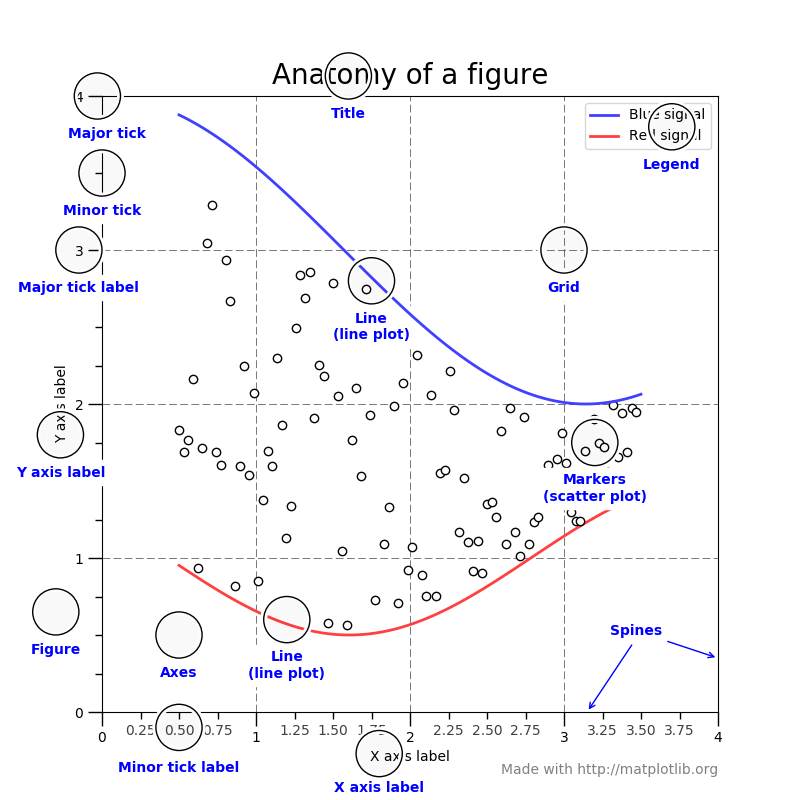
\includegraphics[keepaspectratio]{anatomy.png}}

Galerie wykresów

\url{https://matplotlib.org/gallery/index.html}

\url{https://python-graph-gallery.com/}

\url{https://github.com/rasbt/matplotlib-gallery}

\url{https://seaborn.pydata.org/examples/index.html}

\pandocbounded{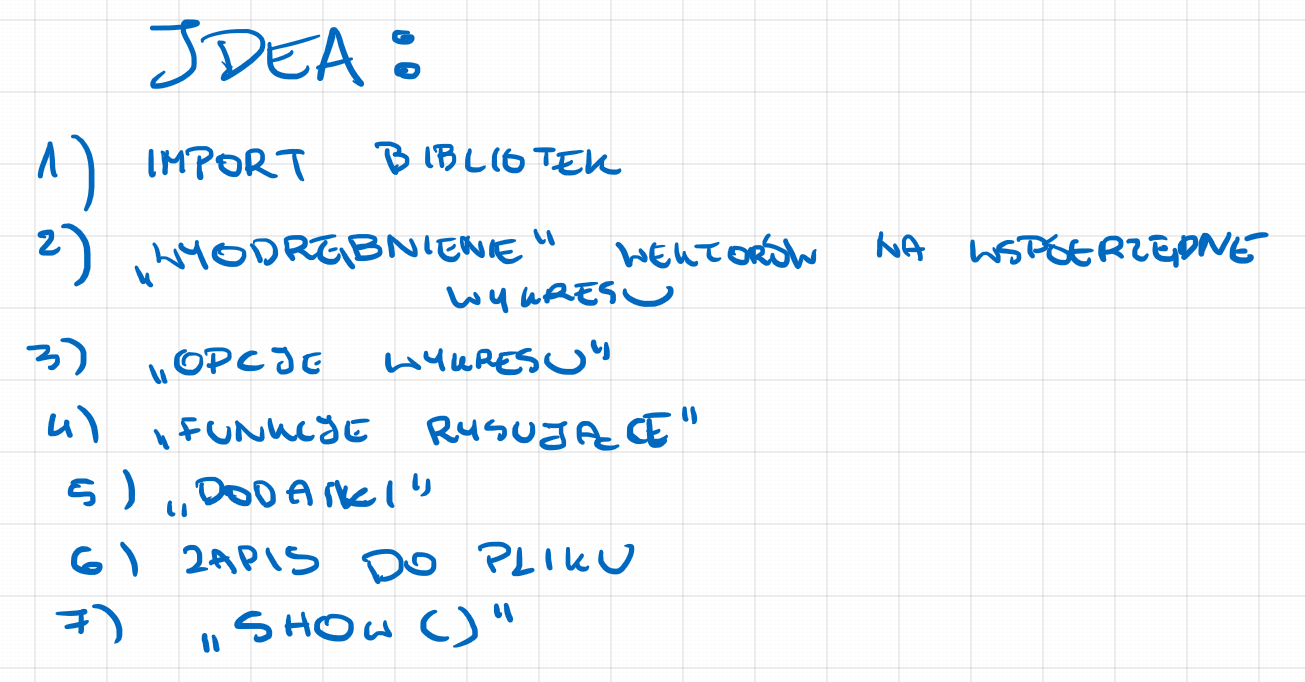
\includegraphics[keepaspectratio]{m1.png}}

\chapter{Matplotlib - wykres liniowy}\label{matplotlib---wykres-liniowy}

Wykres liniowy to jedno z najpotężniejszych narzędzi wizualizacji
danych, które pozwala nam dostrzec zależności i trendy, które mogłyby
pozostać niezauważone w surowych danych. Poniżej przedstawiam
szczegółowe objaśnienie, kiedy i dlaczego warto sięgnąć po ten typ
wykresu.

Wykres liniowy najlepiej sprawdza się, gdy chcemy przedstawić
\textbf{zmiany wartości w czasie} lub w \textbf{funkcji innej zmiennej
ciągłej}. Jego siła tkwi w zdolności do ukazywania ciągłych relacji
między punktami danych, co pozwala na łatwe śledzenie trendów i wzorców.

\begin{enumerate}
\def\labelenumi{\arabic{enumi}.}
\tightlist
\item
  Analiza zmian w czasie
\end{enumerate}

Wykres liniowy doskonale obrazuje, jak dane zmieniają się w kolejnych
jednostkach czasu. Jest nieoceniony przy prezentacji: - Trendów
gospodarczych (wzrost PKB, inflacja, stopy bezrobocia) - Zmian na
rynkach finansowych (kursy walut, ceny akcji, stopy procentowe) - Danych
klimatycznych i pogodowych (zmiany temperatury, opady, poziom
zanieczyszczeń) - Wskaźników zdrowotnych (tętno, poziom cukru we krwi,
ciśnienie)

\begin{enumerate}
\def\labelenumi{\arabic{enumi}.}
\setcounter{enumi}{1}
\tightlist
\item
  Ukazywanie zależności między zmiennymi
\end{enumerate}

Gdy chcemy zbadać, jak jedna zmienna wpływa na drugą, wykres liniowy
pozwala na intuicyjne przedstawienie tych relacji: - Związek między
poziomem wykształcenia a średnimi zarobkami - Korelacja między wiekiem a
określonymi umiejętnościami - Zależność między nakładami na reklamę a
wynikami sprzedaży

\begin{enumerate}
\def\labelenumi{\arabic{enumi}.}
\setcounter{enumi}{2}
\tightlist
\item
  Porównywanie wielu trendów jednocześnie
\end{enumerate}

Wykres liniowy umożliwia efektywne zestawienie kilku serii danych na
jednym wykresie: - Analiza sprzedaży różnych produktów w czasie -
Porównanie wyników różnych regionów, zespołów lub krajów - Zestawienie
faktycznych wyników z planowanymi celami - Porównanie różnych wskaźników
ekonomicznych w tym samym okresie

\begin{enumerate}
\def\labelenumi{\arabic{enumi}.}
\setcounter{enumi}{3}
\tightlist
\item
  Analiza korelacji i przyczynowości
\end{enumerate}

Linie na wykresie pomagają dostrzec, jak zmiany jednej zmiennej mogą
wpływać na inne: - Badanie wpływu cen paliwa na sprzedaż różnych typów
pojazdów - Analiza związku między temperaturą otoczenia a zużyciem
energii - Ocena wpływu kampanii marketingowych na świadomość marki

\begin{enumerate}
\def\labelenumi{\arabic{enumi}.}
\setcounter{enumi}{4}
\tightlist
\item
  Identyfikacja anomalii i punktów zwrotnych
\end{enumerate}

Wykres liniowy pozwala szybko zauważyć wartości odstające oraz momenty
znaczących zmian: - Wykrywanie nietypowych wzorców w danych finansowych
- Identyfikacja punktów przełomowych w trendach społecznych -
Rozpoznawanie sezonowych wahań w danych

Choć wykresy liniowe są najodpowiedniejsze dla danych ciągłych, mogą być
również wykorzystywane do prezentacji danych dyskretnych, o ile istnieje
logiczny związek między kolejnymi punktami. Na przykład, miesięczne
wyniki sprzedaży to dane dyskretne, ale ich przedstawienie w formie
linii pomoże dostrzec trend roczny.

Należy jednak pamiętać, że łączenie punktów linią sugeruje ciągłość
między nimi. Jeśli nie ma logicznej ciągłości między punktami danych
(np. przy porównywaniu niezwiązanych ze sobą kategorii), lepszym wyborem
będzie wykres słupkowy lub punktowy.

\begin{Shaded}
\begin{Highlighting}[]
\ImportTok{import}\NormalTok{ matplotlib.pyplot }\ImportTok{as}\NormalTok{ plt}

\NormalTok{x }\OperatorTok{=}\NormalTok{ [}\DecValTok{0}\NormalTok{, }\DecValTok{7}\NormalTok{, }\DecValTok{4}\NormalTok{, }\DecValTok{5}\NormalTok{, }\DecValTok{8}\NormalTok{, }\OperatorTok{{-}}\DecValTok{9}\NormalTok{]}
\NormalTok{plt.plot(x)}
\NormalTok{plt.show()}
\end{Highlighting}
\end{Shaded}

\pandocbounded{\includegraphics[keepaspectratio]{matplotlib-wykresliniowy_files/figure-pdf/cell-2-output-1.png}}

\phantomsection\label{annotated-cell-155}%
\begin{Shaded}
\begin{Highlighting}[]
\ImportTok{import}\NormalTok{ matplotlib.pyplot }\ImportTok{as}\NormalTok{ plt}
\ImportTok{import}\NormalTok{ numpy }\ImportTok{as}\NormalTok{ np}

\NormalTok{x }\OperatorTok{=}\NormalTok{ np.linspace(}\DecValTok{0}\NormalTok{, }\DecValTok{2}\NormalTok{, }\DecValTok{100}\NormalTok{) }\hspace*{\fill}\NormalTok{\circled{1}}
\NormalTok{plt.plot(x, x, label}\OperatorTok{=}\StringTok{\textquotesingle{}linear\textquotesingle{}}\NormalTok{) }\hspace*{\fill}\NormalTok{\circled{2}}
\NormalTok{plt.plot(x, x }\OperatorTok{**} \DecValTok{2}\NormalTok{, label}\OperatorTok{=}\StringTok{\textquotesingle{}quadratic\textquotesingle{}}\NormalTok{) }\hspace*{\fill}\NormalTok{\circled{3}}
\NormalTok{plt.plot(x, x }\OperatorTok{**} \DecValTok{3}\NormalTok{, label}\OperatorTok{=}\StringTok{\textquotesingle{}cubic\textquotesingle{}}\NormalTok{) }\hspace*{\fill}\NormalTok{\circled{4}}
\NormalTok{plt.xlabel(}\StringTok{\textquotesingle{}x label\textquotesingle{}}\NormalTok{) }\hspace*{\fill}\NormalTok{\circled{5}}
\NormalTok{plt.ylabel(}\StringTok{\textquotesingle{}y label\textquotesingle{}}\NormalTok{) }\hspace*{\fill}\NormalTok{\circled{6}}
\NormalTok{plt.title(}\StringTok{"Simple Plot"}\NormalTok{) }\hspace*{\fill}\NormalTok{\circled{7}}
\NormalTok{plt.legend() }\hspace*{\fill}\NormalTok{\circled{8}}
\NormalTok{plt.show() }\hspace*{\fill}\NormalTok{\circled{9}}
\end{Highlighting}
\end{Shaded}

\begin{description}
\tightlist
\item[\circled{1}]
\texttt{x\ =\ np.linspace(0,\ 2,\ 100)}: tworzy tablicę \texttt{x} z 100
równomiernie rozłożonymi wartościami od 0 do 2 (włącznie), korzystając z
funkcji \texttt{linspace} z biblioteki \texttt{numpy}.
\item[\circled{2}]
\texttt{plt.plot(x,\ x,\ label=\textquotesingle{}linear\textquotesingle{})}:
rysuje liniowy wykres (y = x) z wartościami z tablicy \texttt{x}.
\item[\circled{3}]
\texttt{plt.plot(x,\ x**2,\ label=\textquotesingle{}quadratic\textquotesingle{})}:
rysuje wykres kwadratowy (y = x\^{}2) z wartościami z tablicy
\texttt{x}.
\item[\circled{4}]
\texttt{plt.plot(x,\ x**3,\ label=\textquotesingle{}cubic\textquotesingle{})}:
rysuje wykres sześcienny (y = x\^{}3) z wartościami z tablicy
\texttt{x}.
\item[\circled{5}]
\texttt{plt.xlabel(\textquotesingle{}x\ label\textquotesingle{})}:
dodaje etykietę osi X.
\item[\circled{6}]
\texttt{plt.ylabel(\textquotesingle{}y\ label\textquotesingle{})}:
dodaje etykietę osi Y.
\item[\circled{7}]
\texttt{plt.title("Simple\ Plot")}: nadaje tytuł wykresu ``Simple
Plot''.
\item[\circled{8}]
\texttt{plt.legend()}: dodaje legendę do wykresu, która pokazuje
etykiety (label) dla poszczególnych linii.
\item[\circled{9}]
\texttt{plt.show()}: wyświetla wykres.
\end{description}

\pandocbounded{\includegraphics[keepaspectratio]{matplotlib-wykresliniowy_files/figure-pdf/cell-3-output-1.png}}

Wersja obiektowa:

\begin{Shaded}
\begin{Highlighting}[]
\ImportTok{import}\NormalTok{ matplotlib.pyplot }\ImportTok{as}\NormalTok{ plt}
\ImportTok{import}\NormalTok{ numpy }\ImportTok{as}\NormalTok{ np}

\NormalTok{fig, ax }\OperatorTok{=}\NormalTok{ plt.subplots()}
\NormalTok{x }\OperatorTok{=}\NormalTok{ np.linspace(}\DecValTok{0}\NormalTok{, }\DecValTok{2}\NormalTok{, }\DecValTok{100}\NormalTok{)}

\NormalTok{ax.plot(x, x, label}\OperatorTok{=}\StringTok{\textquotesingle{}linear\textquotesingle{}}\NormalTok{)}
\NormalTok{ax.plot(x, x }\OperatorTok{**} \DecValTok{2}\NormalTok{, label}\OperatorTok{=}\StringTok{\textquotesingle{}quadratic\textquotesingle{}}\NormalTok{)}
\NormalTok{ax.plot(x, x }\OperatorTok{**} \DecValTok{3}\NormalTok{, label}\OperatorTok{=}\StringTok{\textquotesingle{}cubic\textquotesingle{}}\NormalTok{)}

\NormalTok{ax.set\_xlabel(}\StringTok{\textquotesingle{}x label\textquotesingle{}}\NormalTok{)}
\NormalTok{ax.set\_ylabel(}\StringTok{\textquotesingle{}y label\textquotesingle{}}\NormalTok{)}
\NormalTok{ax.set\_title(}\StringTok{"Simple Plot"}\NormalTok{)}

\NormalTok{ax.legend()}
\NormalTok{plt.show()}
\end{Highlighting}
\end{Shaded}

\pandocbounded{\includegraphics[keepaspectratio]{matplotlib-wykresliniowy_files/figure-pdf/cell-4-output-1.png}}

Wersja z datami:

\begin{Shaded}
\begin{Highlighting}[]
\ImportTok{import}\NormalTok{ matplotlib.pyplot }\ImportTok{as}\NormalTok{ plt}
\ImportTok{import}\NormalTok{ numpy }\ImportTok{as}\NormalTok{ np}

\NormalTok{daty }\OperatorTok{=}\NormalTok{ np.arange(}\StringTok{\textquotesingle{}2024{-}01\textquotesingle{}}\NormalTok{, }\StringTok{\textquotesingle{}2025{-}01\textquotesingle{}}\NormalTok{, dtype}\OperatorTok{=}\StringTok{\textquotesingle{}datetime64\textquotesingle{}}\NormalTok{) }

\NormalTok{index }\OperatorTok{=}\NormalTok{ np.arange(}\BuiltInTok{len}\NormalTok{(daty))}

\NormalTok{y\_1 }\OperatorTok{=}\NormalTok{ index}
\NormalTok{y\_2 }\OperatorTok{=}\NormalTok{ index }\OperatorTok{**} \DecValTok{2}
\NormalTok{y\_3 }\OperatorTok{=}\NormalTok{ index }\OperatorTok{**} \DecValTok{3}

\NormalTok{plt.plot(daty, y\_1, label}\OperatorTok{=}\StringTok{\textquotesingle{}Liniowa\textquotesingle{}}\NormalTok{)}
\NormalTok{plt.plot(daty, y\_2, label}\OperatorTok{=}\StringTok{\textquotesingle{}Kwadratowa\textquotesingle{}}\NormalTok{)}
\NormalTok{plt.plot(daty, y\_3, label}\OperatorTok{=}\StringTok{\textquotesingle{}Sześcienna\textquotesingle{}}\NormalTok{)}

\NormalTok{plt.xlabel(}\StringTok{\textquotesingle{}Miesiąc (2024)\textquotesingle{}}\NormalTok{)}
\NormalTok{plt.ylabel(}\StringTok{\textquotesingle{}Wartość\textquotesingle{}}\NormalTok{)}
\NormalTok{plt.title(}\StringTok{"Funkcje w roku 2024"}\NormalTok{)}
\NormalTok{plt.legend()}
\NormalTok{plt.grid(}\VariableTok{True}\NormalTok{)}

\NormalTok{plt.show()}
\end{Highlighting}
\end{Shaded}

\pandocbounded{\includegraphics[keepaspectratio]{matplotlib-wykresliniowy_files/figure-pdf/cell-5-output-1.png}}

\begin{Shaded}
\begin{Highlighting}[]
\ImportTok{import}\NormalTok{ matplotlib.pyplot }\ImportTok{as}\NormalTok{ plt}
\ImportTok{import}\NormalTok{ numpy }\ImportTok{as}\NormalTok{ np}

\CommentTok{\# Tworzenie danych}
\NormalTok{daty }\OperatorTok{=}\NormalTok{ np.arange(}\StringTok{\textquotesingle{}2024{-}01\textquotesingle{}}\NormalTok{, }\StringTok{\textquotesingle{}2025{-}01\textquotesingle{}}\NormalTok{, dtype}\OperatorTok{=}\StringTok{\textquotesingle{}datetime64\textquotesingle{}}\NormalTok{)}
\NormalTok{index }\OperatorTok{=}\NormalTok{ np.arange(}\BuiltInTok{len}\NormalTok{(daty))}
\NormalTok{y\_1 }\OperatorTok{=}\NormalTok{ index}
\NormalTok{y\_2 }\OperatorTok{=}\NormalTok{ index}\OperatorTok{**}\DecValTok{2}
\NormalTok{y\_3 }\OperatorTok{=}\NormalTok{ index}\OperatorTok{**}\DecValTok{3}

\CommentTok{\# Tworzenie figury i osi w podejściu obiektowym}
\NormalTok{fig, ax }\OperatorTok{=}\NormalTok{ plt.subplots()}

\CommentTok{\# Rysowanie linii na osiach}
\NormalTok{ax.plot(daty, y\_1, label}\OperatorTok{=}\StringTok{\textquotesingle{}Liniowa\textquotesingle{}}\NormalTok{)}
\NormalTok{ax.plot(daty, y\_2, label}\OperatorTok{=}\StringTok{\textquotesingle{}Kwadratowa\textquotesingle{}}\NormalTok{)}
\NormalTok{ax.plot(daty, y\_3, label}\OperatorTok{=}\StringTok{\textquotesingle{}Sześcienna\textquotesingle{}}\NormalTok{)}

\CommentTok{\# Dodawanie etykiet i tytułu}
\NormalTok{ax.set\_xlabel(}\StringTok{\textquotesingle{}Miesiąc (2024)\textquotesingle{}}\NormalTok{)}
\NormalTok{ax.set\_ylabel(}\StringTok{\textquotesingle{}Wartość\textquotesingle{}}\NormalTok{)}
\NormalTok{ax.set\_title(}\StringTok{\textquotesingle{}Funkcje w roku 2024\textquotesingle{}}\NormalTok{)}

\CommentTok{\# Dodawanie legendy i siatki}
\NormalTok{ax.legend()}
\NormalTok{ax.grid(}\VariableTok{True}\NormalTok{)}

\CommentTok{\# Dostosowanie wyglądu {-} opcjonalne ulepszenia}
\NormalTok{fig.autofmt\_xdate()  }\CommentTok{\# Automatyczne formatowanie dat na osi X dla lepszej czytelności}
\NormalTok{plt.tight\_layout()   }\CommentTok{\# Automatyczne dostosowanie rozmiaru wykresu}

\CommentTok{\# Wyświetlenie wykresu}
\NormalTok{plt.show()}
\end{Highlighting}
\end{Shaded}

\pandocbounded{\includegraphics[keepaspectratio]{matplotlib-wykresliniowy_files/figure-pdf/cell-6-output-1.png}}

\chapter{Matplotlib - dodatki cz.1}\label{matplotlib---dodatki-cz.1}

\section{Parametry legendy}\label{parametry-legendy}

\pandocbounded{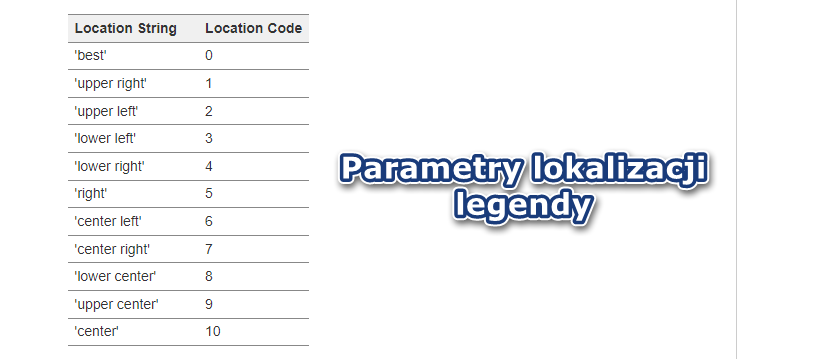
\includegraphics[keepaspectratio]{m2.png}}

\begin{Shaded}
\begin{Highlighting}[]
\ImportTok{import}\NormalTok{ matplotlib.pyplot }\ImportTok{as}\NormalTok{ plt}
\ImportTok{import}\NormalTok{ numpy }\ImportTok{as}\NormalTok{ np}

\NormalTok{x }\OperatorTok{=}\NormalTok{ np.linspace(}\DecValTok{0}\NormalTok{, }\DecValTok{2}\NormalTok{, }\DecValTok{100}\NormalTok{)}
\NormalTok{plt.plot(x, x, label}\OperatorTok{=}\StringTok{\textquotesingle{}linear\textquotesingle{}}\NormalTok{)}
\NormalTok{plt.plot(x, x }\OperatorTok{**} \DecValTok{2}\NormalTok{, label}\OperatorTok{=}\StringTok{\textquotesingle{}quadratic\textquotesingle{}}\NormalTok{)}
\NormalTok{plt.plot(x, x }\OperatorTok{**} \DecValTok{3}\NormalTok{, label}\OperatorTok{=}\StringTok{\textquotesingle{}cubic\textquotesingle{}}\NormalTok{)}
\NormalTok{plt.xlabel(}\StringTok{\textquotesingle{}x label\textquotesingle{}}\NormalTok{)}
\NormalTok{plt.ylabel(}\StringTok{\textquotesingle{}y label\textquotesingle{}}\NormalTok{)}
\NormalTok{plt.title(}\StringTok{"Simple Plot"}\NormalTok{)}
\NormalTok{plt.legend(loc }\OperatorTok{=} \DecValTok{5}\NormalTok{)}
\NormalTok{plt.show()}
\end{Highlighting}
\end{Shaded}

\pandocbounded{\includegraphics[keepaspectratio]{matplotlib-dodatki1_files/figure-pdf/cell-2-output-1.png}}

\begin{Shaded}
\begin{Highlighting}[]
\ImportTok{import}\NormalTok{ matplotlib.pyplot }\ImportTok{as}\NormalTok{ plt}
\ImportTok{import}\NormalTok{ numpy }\ImportTok{as}\NormalTok{ np}

\CommentTok{\# Tworzymy obiekt Figure i osie (Axes)}
\NormalTok{fig }\OperatorTok{=}\NormalTok{ plt.figure()}
\NormalTok{ax }\OperatorTok{=}\NormalTok{ fig.add\_subplot(}\DecValTok{111}\NormalTok{)  }\CommentTok{\# 111 oznacza: 1 wiersz, 1 kolumna, pierwszy wykres}

\CommentTok{\# Generujemy dane}
\NormalTok{x }\OperatorTok{=}\NormalTok{ np.linspace(}\DecValTok{0}\NormalTok{, }\DecValTok{2}\NormalTok{, }\DecValTok{100}\NormalTok{)}

\CommentTok{\# Rysujemy wykresy na osi}
\NormalTok{ax.plot(x, x, label}\OperatorTok{=}\StringTok{\textquotesingle{}linear\textquotesingle{}}\NormalTok{)}
\NormalTok{ax.plot(x, x}\OperatorTok{**}\DecValTok{2}\NormalTok{, label}\OperatorTok{=}\StringTok{\textquotesingle{}quadratic\textquotesingle{}}\NormalTok{)}
\NormalTok{ax.plot(x, x}\OperatorTok{**}\DecValTok{3}\NormalTok{, label}\OperatorTok{=}\StringTok{\textquotesingle{}cubic\textquotesingle{}}\NormalTok{)}

\CommentTok{\# Dodajemy etykiety i tytuł}
\NormalTok{ax.set\_xlabel(}\StringTok{\textquotesingle{}x label\textquotesingle{}}\NormalTok{)}
\NormalTok{ax.set\_ylabel(}\StringTok{\textquotesingle{}y label\textquotesingle{}}\NormalTok{)}
\NormalTok{ax.set\_title(}\StringTok{"Simple Plot"}\NormalTok{)}

\CommentTok{\# Dodajemy legendę}
\NormalTok{ax.legend(loc}\OperatorTok{=}\DecValTok{5}\NormalTok{)  }\CommentTok{\# loc=5 oznacza położenie "right"}

\CommentTok{\# Wyświetlamy wykres}
\NormalTok{plt.show()}
\end{Highlighting}
\end{Shaded}

\pandocbounded{\includegraphics[keepaspectratio]{matplotlib-dodatki1_files/figure-pdf/cell-3-output-1.png}}

\section{Style, kolory linii}\label{style-kolory-linii}

\phantomsection\label{annotated-cell-161}%
\begin{Shaded}
\begin{Highlighting}[]
\ImportTok{import}\NormalTok{ numpy }\ImportTok{as}\NormalTok{ np}
\ImportTok{import}\NormalTok{ matplotlib.pyplot }\ImportTok{as}\NormalTok{ plt}

\NormalTok{x }\OperatorTok{=}\NormalTok{ np.arange(}\DecValTok{14}\NormalTok{) }\hspace*{\fill}\NormalTok{\circled{1}}
\NormalTok{y }\OperatorTok{=}\NormalTok{ np.cos(}\DecValTok{5} \OperatorTok{*}\NormalTok{ x) }\hspace*{\fill}\NormalTok{\circled{2}}
\NormalTok{plt.plot(x, y }\OperatorTok{+} \DecValTok{2}\NormalTok{, }\StringTok{\textquotesingle{}blue\textquotesingle{}}\NormalTok{, linestyle}\OperatorTok{=}\StringTok{"{-}"}\NormalTok{, label}\OperatorTok{=}\StringTok{"niebieski"}\NormalTok{) }\hspace*{\fill}\NormalTok{\circled{3}}
\NormalTok{plt.plot(x, y }\OperatorTok{+} \DecValTok{1}\NormalTok{, }\StringTok{\textquotesingle{}red\textquotesingle{}}\NormalTok{, linestyle}\OperatorTok{=}\StringTok{":"}\NormalTok{, label}\OperatorTok{=}\StringTok{"czerwony"}\NormalTok{) }\hspace*{\fill}\NormalTok{\circled{4}}
\NormalTok{plt.plot(x, y, }\StringTok{\textquotesingle{}green\textquotesingle{}}\NormalTok{, linestyle}\OperatorTok{=}\StringTok{"{-}{-}"}\NormalTok{, label}\OperatorTok{=}\StringTok{"zielony"}\NormalTok{) }\hspace*{\fill}\NormalTok{\circled{5}}
\NormalTok{plt.legend(title}\OperatorTok{=}\StringTok{\textquotesingle{}Legenda:\textquotesingle{}}\NormalTok{)}
\NormalTok{plt.show()}
\end{Highlighting}
\end{Shaded}

\begin{description}
\tightlist
\item[\circled{1}]
\texttt{x\ =\ np.arange(14)}: tworzy tablicę \texttt{x} z wartościami od
0 do 13 (łącznie z 13), korzystając z funkcji \texttt{arange} z
biblioteki \texttt{numpy}.
\item[\circled{2}]
\texttt{y\ =\ np.cos(5\ *\ x)}: oblicza wartości funkcji cosinus dla
każdej wartości \texttt{x}, przemnożonej przez 5. Wynikowe wartości są
zapisane w tablicy \texttt{y}.
\item[\circled{3}]
\texttt{plt.plot(x,\ y\ +\ 2,\ \textquotesingle{}blue\textquotesingle{},\ linestyle="-",\ label="niebieski")}:
rysuje niebieski wykres z wartościami z tablicy \texttt{x}, a wartości
\texttt{y} przesunięte o 2 w górę. Linia jest ciągła
(\texttt{linestyle="-"}).
\item[\circled{4}]
\texttt{plt.plot(x,\ y\ +\ 1,\ \textquotesingle{}red\textquotesingle{},\ linestyle=":",\ label="czerwony")}:
rysuje czerwony wykres z wartościami z tablicy \texttt{x}, a wartości
\texttt{y} przesunięte o 1 w górę. Linia jest punktowana
(\texttt{linestyle=":"}).
\item[\circled{5}]
\texttt{plt.plot(x,\ y,\ \textquotesingle{}green\textquotesingle{},\ linestyle="-\/-",\ label="zielony")}:
rysuje zielony wykres z wartościami z tablicy \texttt{x} i wartościami
\texttt{y}. Linia jest przerywana (\texttt{linestyle="-\/-"}).
\end{description}

\pandocbounded{\includegraphics[keepaspectratio]{matplotlib-dodatki1_files/figure-pdf/cell-4-output-1.png}}

\pandocbounded{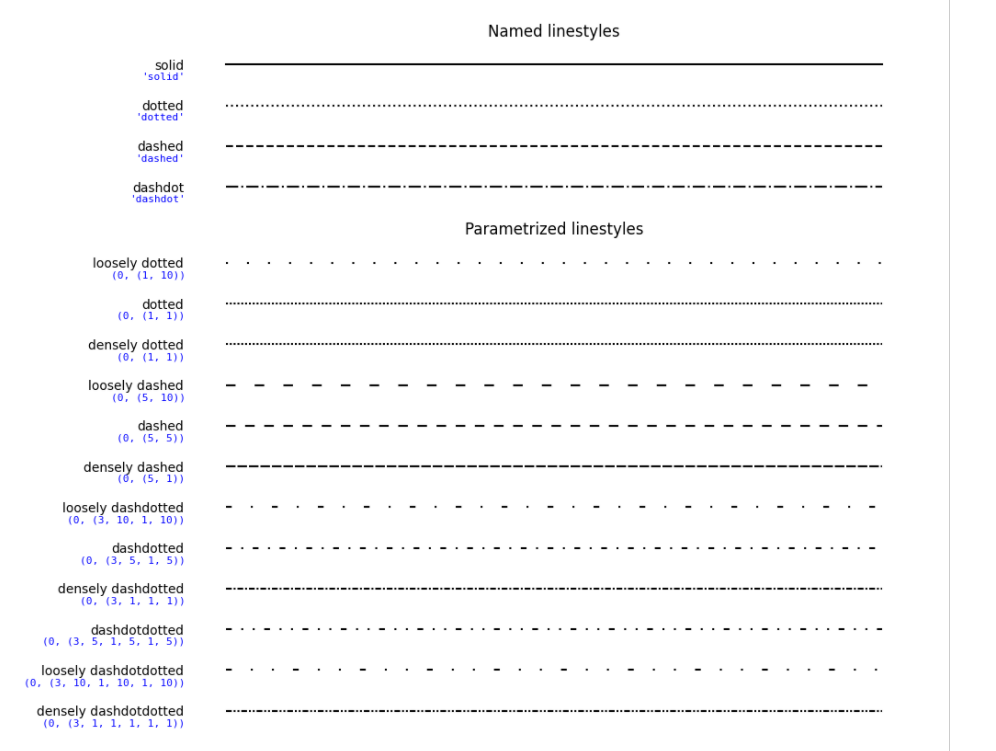
\includegraphics[keepaspectratio]{m3.png}}

\pandocbounded{
\includegraphics[keepaspectratio]{m4.png}}

\pandocbounded{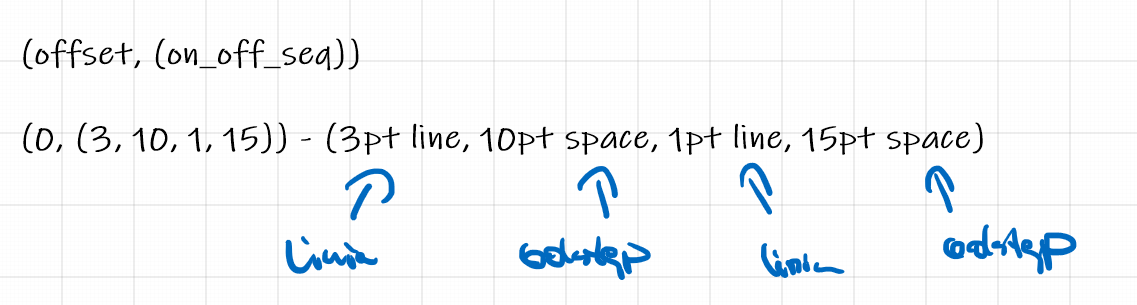
\includegraphics[keepaspectratio]{m5.png}}

\begin{Shaded}
\begin{Highlighting}[]
\ImportTok{import}\NormalTok{ numpy }\ImportTok{as}\NormalTok{ np}
\ImportTok{import}\NormalTok{ matplotlib.pyplot }\ImportTok{as}\NormalTok{ plt}

\NormalTok{fig }\OperatorTok{=}\NormalTok{ plt.figure()}
\NormalTok{ax }\OperatorTok{=}\NormalTok{ fig.add\_subplot(}\DecValTok{111}\NormalTok{)}

\NormalTok{x }\OperatorTok{=}\NormalTok{ np.arange(}\DecValTok{14}\NormalTok{)}
\NormalTok{y }\OperatorTok{=}\NormalTok{ np.cos(}\DecValTok{5} \OperatorTok{*}\NormalTok{ x)}

\NormalTok{ax.plot(x, y }\OperatorTok{+} \DecValTok{2}\NormalTok{, }\StringTok{\textquotesingle{}blue\textquotesingle{}}\NormalTok{, linestyle}\OperatorTok{=}\StringTok{"{-}"}\NormalTok{, label}\OperatorTok{=}\StringTok{"niebieski"}\NormalTok{)}
\NormalTok{ax.plot(x, y }\OperatorTok{+} \DecValTok{1}\NormalTok{, }\StringTok{\textquotesingle{}red\textquotesingle{}}\NormalTok{, linestyle}\OperatorTok{=}\StringTok{":"}\NormalTok{, label}\OperatorTok{=}\StringTok{"czerwony"}\NormalTok{)}
\NormalTok{ax.plot(x, y, }\StringTok{\textquotesingle{}green\textquotesingle{}}\NormalTok{, linestyle}\OperatorTok{=}\StringTok{"{-}{-}"}\NormalTok{, label}\OperatorTok{=}\StringTok{"zielony"}\NormalTok{)}

\NormalTok{ax.legend(title}\OperatorTok{=}\StringTok{\textquotesingle{}Legenda:\textquotesingle{}}\NormalTok{)}

\NormalTok{plt.show()}
\end{Highlighting}
\end{Shaded}

\pandocbounded{\includegraphics[keepaspectratio]{matplotlib-dodatki1_files/figure-pdf/cell-5-output-1.png}}

\begin{Shaded}
\begin{Highlighting}[]
\ImportTok{import}\NormalTok{ matplotlib.pyplot }\ImportTok{as}\NormalTok{ plt}
\ImportTok{import}\NormalTok{ numpy }\ImportTok{as}\NormalTok{ np}

\NormalTok{miesiace }\OperatorTok{=}\NormalTok{ [}\StringTok{\textquotesingle{}Sty\textquotesingle{}}\NormalTok{, }\StringTok{\textquotesingle{}Lut\textquotesingle{}}\NormalTok{, }\StringTok{\textquotesingle{}Mar\textquotesingle{}}\NormalTok{, }\StringTok{\textquotesingle{}Kwi\textquotesingle{}}\NormalTok{, }\StringTok{\textquotesingle{}Maj\textquotesingle{}}\NormalTok{, }\StringTok{\textquotesingle{}Cze\textquotesingle{}}\NormalTok{]}
\NormalTok{sprzedaz }\OperatorTok{=}\NormalTok{ [}\DecValTok{12500}\NormalTok{, }\DecValTok{14000}\NormalTok{, }\DecValTok{16700}\NormalTok{, }\DecValTok{15400}\NormalTok{, }\DecValTok{18200}\NormalTok{, }\DecValTok{19500}\NormalTok{]}

\NormalTok{plt.plot(miesiace, sprzedaz, }\StringTok{\textquotesingle{}bo{-}\textquotesingle{}}\NormalTok{, linewidth}\OperatorTok{=}\DecValTok{2}\NormalTok{, markersize}\OperatorTok{=}\DecValTok{8}\NormalTok{)}
\NormalTok{plt.grid(}\VariableTok{True}\NormalTok{, linestyle}\OperatorTok{=}\StringTok{\textquotesingle{}{-}{-}\textquotesingle{}}\NormalTok{, alpha}\OperatorTok{=}\FloatTok{0.7}\NormalTok{)}
\NormalTok{plt.title(}\StringTok{\textquotesingle{}Sprzedaż w pierwszym półroczu 2025\textquotesingle{}}\NormalTok{)}
\NormalTok{plt.xlabel(}\StringTok{\textquotesingle{}Miesiąc\textquotesingle{}}\NormalTok{)}
\NormalTok{plt.ylabel(}\StringTok{\textquotesingle{}Sprzedaż (PLN)\textquotesingle{}}\NormalTok{)}
\NormalTok{plt.ylim([}\DecValTok{10000}\NormalTok{, }\DecValTok{21000}\NormalTok{])}
\NormalTok{plt.fill\_between(miesiace, sprzedaz, }\DecValTok{10000}\NormalTok{, alpha}\OperatorTok{=}\FloatTok{0.2}\NormalTok{, color}\OperatorTok{=}\StringTok{\textquotesingle{}skyblue\textquotesingle{}}\NormalTok{)}
\NormalTok{plt.axhline(y}\OperatorTok{=}\DecValTok{15000}\NormalTok{, color}\OperatorTok{=}\StringTok{\textquotesingle{}red\textquotesingle{}}\NormalTok{, linestyle}\OperatorTok{=}\StringTok{\textquotesingle{}{-}{-}\textquotesingle{}}\NormalTok{)}
\NormalTok{plt.text(}\DecValTok{0}\NormalTok{, }\DecValTok{15300}\NormalTok{, }\StringTok{\textquotesingle{}Cel miesięczny\textquotesingle{}}\NormalTok{, color}\OperatorTok{=}\StringTok{\textquotesingle{}red\textquotesingle{}}\NormalTok{)}
\NormalTok{plt.tight\_layout()}
\NormalTok{plt.show()}
\end{Highlighting}
\end{Shaded}

\pandocbounded{\includegraphics[keepaspectratio]{matplotlib-dodatki1_files/figure-pdf/cell-6-output-1.png}}

\begin{Shaded}
\begin{Highlighting}[]
\ImportTok{import}\NormalTok{ matplotlib.pyplot }\ImportTok{as}\NormalTok{ plt}
\ImportTok{import}\NormalTok{ numpy }\ImportTok{as}\NormalTok{ np}

\NormalTok{miesiace }\OperatorTok{=}\NormalTok{ [}\StringTok{\textquotesingle{}Sty\textquotesingle{}}\NormalTok{, }\StringTok{\textquotesingle{}Lut\textquotesingle{}}\NormalTok{, }\StringTok{\textquotesingle{}Mar\textquotesingle{}}\NormalTok{, }\StringTok{\textquotesingle{}Kwi\textquotesingle{}}\NormalTok{, }\StringTok{\textquotesingle{}Maj\textquotesingle{}}\NormalTok{, }\StringTok{\textquotesingle{}Cze\textquotesingle{}}\NormalTok{]}
\NormalTok{sprzedaz }\OperatorTok{=}\NormalTok{ [}\DecValTok{12500}\NormalTok{, }\DecValTok{14000}\NormalTok{, }\DecValTok{16700}\NormalTok{, }\DecValTok{15400}\NormalTok{, }\DecValTok{18200}\NormalTok{, }\DecValTok{19500}\NormalTok{]}

\NormalTok{fig, ax }\OperatorTok{=}\NormalTok{ plt.subplots()}
\NormalTok{ax.plot(miesiace, sprzedaz, }\StringTok{\textquotesingle{}bo{-}\textquotesingle{}}\NormalTok{, linewidth}\OperatorTok{=}\DecValTok{2}\NormalTok{, markersize}\OperatorTok{=}\DecValTok{8}\NormalTok{)}
\NormalTok{ax.grid(}\VariableTok{True}\NormalTok{, linestyle}\OperatorTok{=}\StringTok{\textquotesingle{}{-}{-}\textquotesingle{}}\NormalTok{, alpha}\OperatorTok{=}\FloatTok{0.7}\NormalTok{)}
\NormalTok{ax.set\_title(}\StringTok{\textquotesingle{}Sprzedaż w pierwszym półroczu 2025\textquotesingle{}}\NormalTok{)}
\NormalTok{ax.set\_xlabel(}\StringTok{\textquotesingle{}Miesiąc\textquotesingle{}}\NormalTok{)}
\NormalTok{ax.set\_ylabel(}\StringTok{\textquotesingle{}Sprzedaż (PLN)\textquotesingle{}}\NormalTok{)}
\NormalTok{ax.set\_ylim([}\DecValTok{10000}\NormalTok{, }\DecValTok{21000}\NormalTok{])}
\NormalTok{ax.fill\_between(miesiace, sprzedaz, }\DecValTok{10000}\NormalTok{, alpha}\OperatorTok{=}\FloatTok{0.2}\NormalTok{, color}\OperatorTok{=}\StringTok{\textquotesingle{}skyblue\textquotesingle{}}\NormalTok{)}
\NormalTok{ax.axhline(y}\OperatorTok{=}\DecValTok{15000}\NormalTok{, color}\OperatorTok{=}\StringTok{\textquotesingle{}red\textquotesingle{}}\NormalTok{, linestyle}\OperatorTok{=}\StringTok{\textquotesingle{}{-}{-}\textquotesingle{}}\NormalTok{)}
\NormalTok{ax.text(}\DecValTok{0}\NormalTok{, }\DecValTok{15300}\NormalTok{, }\StringTok{\textquotesingle{}Cel miesięczny\textquotesingle{}}\NormalTok{, color}\OperatorTok{=}\StringTok{\textquotesingle{}red\textquotesingle{}}\NormalTok{)}
\NormalTok{plt.tight\_layout()}
\NormalTok{plt.show()}
\end{Highlighting}
\end{Shaded}

\pandocbounded{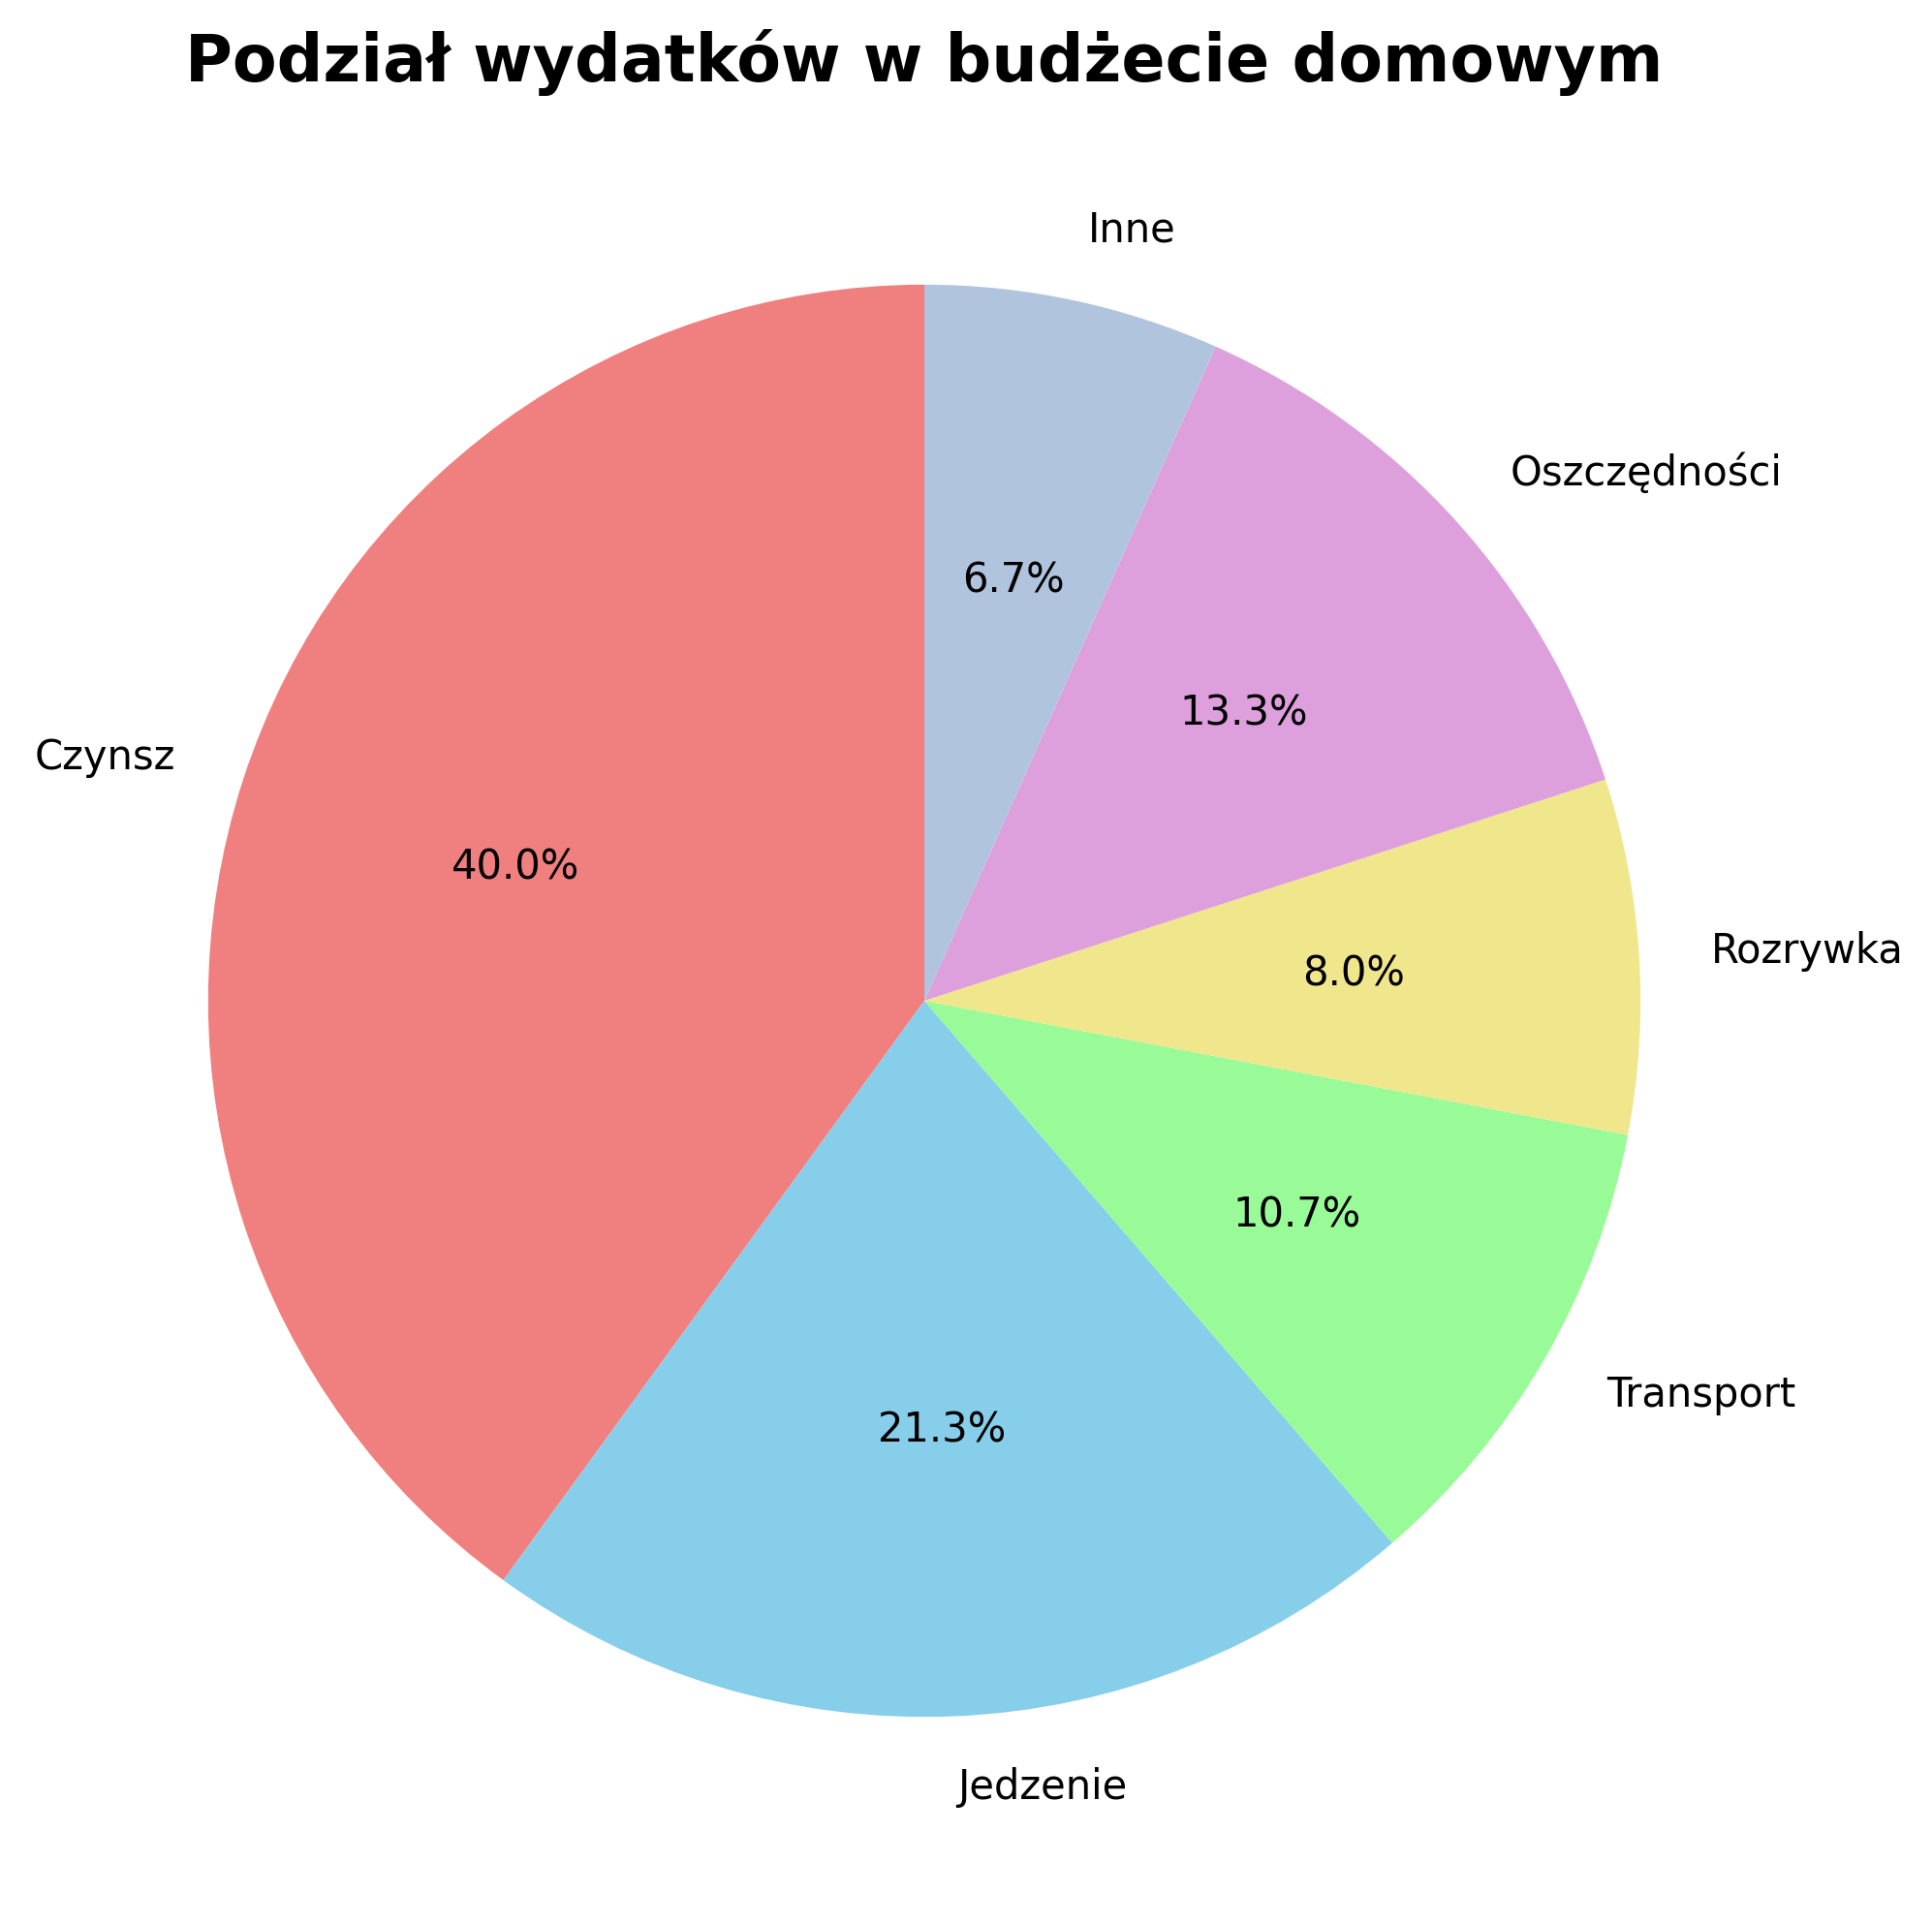
\includegraphics[keepaspectratio]{matplotlib-dodatki1_files/figure-pdf/cell-7-output-1.png}}

\chapter{Matplotlib - podwykresy}\label{matplotlib---podwykresy}

\pandocbounded{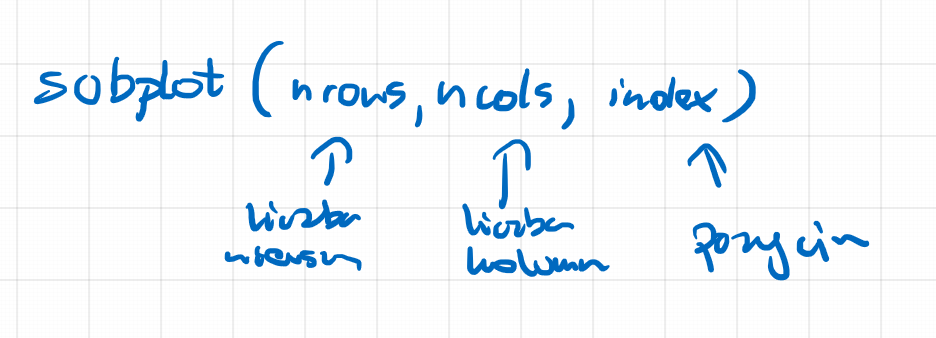
\includegraphics[keepaspectratio]{m8.png}}

Funkcja \texttt{subplot} pozwala na tworzenie wielu wykresów w
pojedynczym oknie lub figurze. Dzięki temu można porównać różne wykresy,
które mają wspólny kontekst lub prezentować różne aspekty danych.

Składnia funkcji to
\texttt{plt.subplot(nrows,\ ncols,\ index,\ **kwargs)}, gdzie:

\begin{itemize}
\tightlist
\item
  \texttt{nrows} - liczba wierszy w siatce wykresów.
\item
  \texttt{ncols} - liczba kolumn w siatce wykresów.
\item
  \texttt{index} - indeks bieżącego wykresu, który ma być utworzony
  (indeksacja zaczyna się od 1). Indeksy są numerowane wierszami, tzn.
  kolejny wykres w rzędzie będzie miał indeks o jeden większy.
\item
  \texttt{**kwargs} - dodatkowe argumenty dotyczące formatowania
  wykresu.
\end{itemize}

\begin{Shaded}
\begin{Highlighting}[]
\ImportTok{import}\NormalTok{ matplotlib.pyplot }\ImportTok{as}\NormalTok{ plt}
\ImportTok{import}\NormalTok{ numpy }\ImportTok{as}\NormalTok{ np}

\NormalTok{x }\OperatorTok{=}\NormalTok{ np.linspace(}\DecValTok{0}\NormalTok{, }\DecValTok{2} \OperatorTok{*}\NormalTok{ np.pi, }\DecValTok{100}\NormalTok{)}

\CommentTok{\# Tworzenie siatki wykresów 2x2}
\CommentTok{\# Pierwszy wykres (w lewym górnym rogu)}
\NormalTok{plt.subplot(}\DecValTok{2}\NormalTok{, }\DecValTok{2}\NormalTok{, }\DecValTok{1}\NormalTok{)}
\NormalTok{plt.plot(x, np.sin(x))}
\NormalTok{plt.title(}\StringTok{\textquotesingle{}sin(x)\textquotesingle{}}\NormalTok{)}

\CommentTok{\# Drugi wykres (w prawym górnym rogu)}
\NormalTok{plt.subplot(}\DecValTok{2}\NormalTok{, }\DecValTok{2}\NormalTok{, }\DecValTok{2}\NormalTok{)}
\NormalTok{plt.plot(x, np.cos(x))}
\NormalTok{plt.title(}\StringTok{\textquotesingle{}cos(x)\textquotesingle{}}\NormalTok{)}

\CommentTok{\# Trzeci wykres (w lewym dolnym rogu)}
\NormalTok{plt.subplot(}\DecValTok{2}\NormalTok{, }\DecValTok{2}\NormalTok{, }\DecValTok{3}\NormalTok{)}
\NormalTok{plt.plot(x, np.tan(x))}
\NormalTok{plt.title(}\StringTok{\textquotesingle{}tan(x)\textquotesingle{}}\NormalTok{)}

\CommentTok{\# Czwarty wykres (w prawym dolnym rogu)}
\NormalTok{plt.subplot(}\DecValTok{2}\NormalTok{, }\DecValTok{2}\NormalTok{, }\DecValTok{4}\NormalTok{)}
\NormalTok{plt.plot(x, }\OperatorTok{{-}}\NormalTok{np.sin(x))}
\NormalTok{plt.title(}\StringTok{\textquotesingle{}{-}sin(x)\textquotesingle{}}\NormalTok{)}

\CommentTok{\# Dopasowanie odstępów między wykresami}
\NormalTok{plt.tight\_layout()}

\CommentTok{\# Wyświetlenie wykresów}
\NormalTok{plt.show()}
\end{Highlighting}
\end{Shaded}

\pandocbounded{\includegraphics[keepaspectratio]{matplotlib-podwykresy_files/figure-pdf/cell-2-output-1.png}}

\begin{Shaded}
\begin{Highlighting}[]
\ImportTok{import}\NormalTok{ numpy }\ImportTok{as}\NormalTok{ np}
\ImportTok{import}\NormalTok{ matplotlib.pyplot }\ImportTok{as}\NormalTok{ plt}

\NormalTok{x }\OperatorTok{=}\NormalTok{ np.arange(}\DecValTok{0}\NormalTok{, }\DecValTok{3}\NormalTok{, }\FloatTok{0.1}\NormalTok{)}
\NormalTok{plt.subplot(}\DecValTok{2}\NormalTok{, }\DecValTok{2}\NormalTok{, }\DecValTok{1}\NormalTok{)}
\NormalTok{plt.plot(x, x)}
\NormalTok{plt.subplot(}\DecValTok{2}\NormalTok{, }\DecValTok{2}\NormalTok{, }\DecValTok{2}\NormalTok{)}
\NormalTok{plt.plot(x, x }\OperatorTok{*} \DecValTok{2}\NormalTok{)}
\NormalTok{plt.subplot(}\DecValTok{2}\NormalTok{, }\DecValTok{2}\NormalTok{, }\DecValTok{3}\NormalTok{)}
\NormalTok{plt.plot(x, x }\OperatorTok{*}\NormalTok{ x)}
\NormalTok{plt.subplot(}\DecValTok{2}\NormalTok{, }\DecValTok{2}\NormalTok{, }\DecValTok{4}\NormalTok{)}
\NormalTok{plt.plot(x, x }\OperatorTok{**} \DecValTok{3}\NormalTok{)}
\NormalTok{plt.tight\_layout()}
\NormalTok{plt.show()}
\end{Highlighting}
\end{Shaded}

\pandocbounded{\includegraphics[keepaspectratio]{matplotlib-podwykresy_files/figure-pdf/cell-3-output-1.png}}

\begin{Shaded}
\begin{Highlighting}[]
\ImportTok{import}\NormalTok{ numpy }\ImportTok{as}\NormalTok{ np}
\ImportTok{import}\NormalTok{ matplotlib.pyplot }\ImportTok{as}\NormalTok{ plt}

\NormalTok{x }\OperatorTok{=}\NormalTok{ np.arange(}\DecValTok{0}\NormalTok{, }\DecValTok{3}\NormalTok{, }\FloatTok{0.1}\NormalTok{)}

\NormalTok{fig, axes }\OperatorTok{=}\NormalTok{ plt.subplots(}\DecValTok{2}\NormalTok{, }\DecValTok{2}\NormalTok{)}

\NormalTok{axes[}\DecValTok{0}\NormalTok{, }\DecValTok{0}\NormalTok{].plot(x, x)}
\NormalTok{axes[}\DecValTok{0}\NormalTok{, }\DecValTok{1}\NormalTok{].plot(x, x }\OperatorTok{*} \DecValTok{2}\NormalTok{)}
\NormalTok{axes[}\DecValTok{1}\NormalTok{, }\DecValTok{0}\NormalTok{].plot(x, x }\OperatorTok{*}\NormalTok{ x)}
\NormalTok{axes[}\DecValTok{1}\NormalTok{, }\DecValTok{1}\NormalTok{].plot(x, x }\OperatorTok{**} \DecValTok{3}\NormalTok{)}

\NormalTok{fig.tight\_layout()}
\NormalTok{plt.show()}
\end{Highlighting}
\end{Shaded}

\pandocbounded{\includegraphics[keepaspectratio]{matplotlib-podwykresy_files/figure-pdf/cell-4-output-1.png}}

\begin{Shaded}
\begin{Highlighting}[]
\ImportTok{import}\NormalTok{ numpy }\ImportTok{as}\NormalTok{ np}
\ImportTok{import}\NormalTok{ matplotlib.pyplot }\ImportTok{as}\NormalTok{ plt}

\CommentTok{\# Przygotowanie danych do wizualizacji}
\NormalTok{x }\OperatorTok{=}\NormalTok{ np.linspace(}\DecValTok{0}\NormalTok{, }\DecValTok{10}\NormalTok{, }\DecValTok{100}\NormalTok{)  }\CommentTok{\# Tworzymy 100 punktów w zakresie od 0 do 10}
\NormalTok{y1 }\OperatorTok{=}\NormalTok{ np.sin(x)               }\CommentTok{\# Funkcja sinus}
\NormalTok{y2 }\OperatorTok{=}\NormalTok{ np.cos(x)               }\CommentTok{\# Funkcja cosinus}
\NormalTok{y3 }\OperatorTok{=}\NormalTok{ np.exp(}\OperatorTok{{-}}\FloatTok{0.2}\OperatorTok{*}\NormalTok{x) }\OperatorTok{*}\NormalTok{ np.sin(x)  }\CommentTok{\# Funkcja tłumionego sinusa}
\NormalTok{y4 }\OperatorTok{=}\NormalTok{ x}\OperatorTok{**}\DecValTok{2} \OperatorTok{/} \DecValTok{20}               \CommentTok{\# Funkcja kwadratowa}

\CommentTok{\# Tworzenie figury i podwykresów (2 rzędy, 2 kolumny)}
\CommentTok{\# W podejściu proceduralnym używamy pyplot bezpośrednio}
\NormalTok{plt.figure(figsize}\OperatorTok{=}\NormalTok{(}\DecValTok{12}\NormalTok{, }\DecValTok{8}\NormalTok{))  }\CommentTok{\# Ustawiamy rozmiar całej figury (szerokość, wysokość w calach)}

\CommentTok{\# Pierwszy podwykres (lewy górny)}
\NormalTok{plt.subplot(}\DecValTok{2}\NormalTok{, }\DecValTok{2}\NormalTok{, }\DecValTok{1}\NormalTok{)  }\CommentTok{\# 2 rzędy, 2 kolumny, pozycja 1}
\NormalTok{plt.plot(x, y1, }\StringTok{\textquotesingle{}r{-}\textquotesingle{}}\NormalTok{, linewidth}\OperatorTok{=}\DecValTok{2}\NormalTok{)  }\CommentTok{\# Czerwona linia}
\NormalTok{plt.title(}\StringTok{\textquotesingle{}Funkcja sinus\textquotesingle{}}\NormalTok{)}
\NormalTok{plt.xlabel(}\StringTok{\textquotesingle{}X\textquotesingle{}}\NormalTok{)}
\NormalTok{plt.ylabel(}\StringTok{\textquotesingle{}sin(x)\textquotesingle{}}\NormalTok{)}
\NormalTok{plt.grid(}\VariableTok{True}\NormalTok{)  }\CommentTok{\# Dodajemy siatkę}
\NormalTok{plt.axhline(y}\OperatorTok{=}\DecValTok{0}\NormalTok{, color}\OperatorTok{=}\StringTok{\textquotesingle{}k\textquotesingle{}}\NormalTok{, linestyle}\OperatorTok{=}\StringTok{\textquotesingle{}{-}\textquotesingle{}}\NormalTok{, alpha}\OperatorTok{=}\FloatTok{0.3}\NormalTok{)  }\CommentTok{\# Linia pozioma na y=0}

\CommentTok{\# Drugi podwykres (prawy górny)}
\NormalTok{plt.subplot(}\DecValTok{2}\NormalTok{, }\DecValTok{2}\NormalTok{, }\DecValTok{2}\NormalTok{)  }\CommentTok{\# 2 rzędy, 2 kolumny, pozycja 2}
\NormalTok{plt.plot(x, y2, }\StringTok{\textquotesingle{}b{-}\textquotesingle{}}\NormalTok{, linewidth}\OperatorTok{=}\DecValTok{2}\NormalTok{)  }\CommentTok{\# Niebieska linia}
\NormalTok{plt.title(}\StringTok{\textquotesingle{}Funkcja cosinus\textquotesingle{}}\NormalTok{)}
\NormalTok{plt.xlabel(}\StringTok{\textquotesingle{}X\textquotesingle{}}\NormalTok{)}
\NormalTok{plt.ylabel(}\StringTok{\textquotesingle{}cos(x)\textquotesingle{}}\NormalTok{)}
\NormalTok{plt.grid(}\VariableTok{True}\NormalTok{)}
\NormalTok{plt.axhline(y}\OperatorTok{=}\DecValTok{0}\NormalTok{, color}\OperatorTok{=}\StringTok{\textquotesingle{}k\textquotesingle{}}\NormalTok{, linestyle}\OperatorTok{=}\StringTok{\textquotesingle{}{-}\textquotesingle{}}\NormalTok{, alpha}\OperatorTok{=}\FloatTok{0.3}\NormalTok{)}

\CommentTok{\# Trzeci podwykres (lewy dolny)}
\NormalTok{plt.subplot(}\DecValTok{2}\NormalTok{, }\DecValTok{2}\NormalTok{, }\DecValTok{3}\NormalTok{)  }\CommentTok{\# 2 rzędy, 2 kolumny, pozycja 3}
\NormalTok{plt.plot(x, y3, }\StringTok{\textquotesingle{}g{-}\textquotesingle{}}\NormalTok{, linewidth}\OperatorTok{=}\DecValTok{2}\NormalTok{)  }\CommentTok{\# Zielona linia}
\NormalTok{plt.title(}\StringTok{\textquotesingle{}Tłumiony sinus\textquotesingle{}}\NormalTok{)}
\NormalTok{plt.xlabel(}\StringTok{\textquotesingle{}X\textquotesingle{}}\NormalTok{)}
\NormalTok{plt.ylabel(}\StringTok{\textquotesingle{}exp({-}0.2x) * sin(x)\textquotesingle{}}\NormalTok{)}
\NormalTok{plt.grid(}\VariableTok{True}\NormalTok{)}
\NormalTok{plt.axhline(y}\OperatorTok{=}\DecValTok{0}\NormalTok{, color}\OperatorTok{=}\StringTok{\textquotesingle{}k\textquotesingle{}}\NormalTok{, linestyle}\OperatorTok{=}\StringTok{\textquotesingle{}{-}\textquotesingle{}}\NormalTok{, alpha}\OperatorTok{=}\FloatTok{0.3}\NormalTok{)}

\CommentTok{\# Czwarty podwykres (prawy dolny)}
\NormalTok{plt.subplot(}\DecValTok{2}\NormalTok{, }\DecValTok{2}\NormalTok{, }\DecValTok{4}\NormalTok{)  }\CommentTok{\# 2 rzędy, 2 kolumny, pozycja 4}
\NormalTok{plt.plot(x, y4, }\StringTok{\textquotesingle{}orange\textquotesingle{}}\NormalTok{, linewidth}\OperatorTok{=}\DecValTok{2}\NormalTok{, linestyle}\OperatorTok{=}\StringTok{\textquotesingle{}{-}{-}\textquotesingle{}}\NormalTok{, marker}\OperatorTok{=}\StringTok{\textquotesingle{}o\textquotesingle{}}\NormalTok{, markevery}\OperatorTok{=}\DecValTok{10}\NormalTok{, markersize}\OperatorTok{=}\DecValTok{5}\NormalTok{)}
\NormalTok{plt.title(}\StringTok{\textquotesingle{}Funkcja kwadratowa\textquotesingle{}}\NormalTok{)}
\NormalTok{plt.xlabel(}\StringTok{\textquotesingle{}X\textquotesingle{}}\NormalTok{)}
\NormalTok{plt.ylabel(}\StringTok{\textquotesingle{}x²/20\textquotesingle{}}\NormalTok{)}
\NormalTok{plt.grid(}\VariableTok{True}\NormalTok{)}

\CommentTok{\# Dodanie adnotacji na ostatnim wykresie}
\NormalTok{plt.annotate(}\StringTok{\textquotesingle{}Punkt (5, 1.25)\textquotesingle{}}\NormalTok{, xy}\OperatorTok{=}\NormalTok{(}\DecValTok{5}\NormalTok{, }\FloatTok{1.25}\NormalTok{), xytext}\OperatorTok{=}\NormalTok{(}\DecValTok{6}\NormalTok{, }\FloatTok{1.8}\NormalTok{),}
\NormalTok{             arrowprops}\OperatorTok{=}\BuiltInTok{dict}\NormalTok{(facecolor}\OperatorTok{=}\StringTok{\textquotesingle{}black\textquotesingle{}}\NormalTok{, shrink}\OperatorTok{=}\FloatTok{0.05}\NormalTok{, width}\OperatorTok{=}\FloatTok{1.5}\NormalTok{))}

\CommentTok{\# Dostosowanie układu wykresów {-} zapobiega nakładaniu się}
\NormalTok{plt.tight\_layout()}

\CommentTok{\# Dodanie ogólnego tytułu dla całej figury}
\NormalTok{plt.suptitle(}\StringTok{\textquotesingle{}Przykład wykresów z podwykresami {-} podejście proceduralne\textquotesingle{}}\NormalTok{, fontsize}\OperatorTok{=}\DecValTok{16}\NormalTok{)}
\NormalTok{plt.subplots\_adjust(top}\OperatorTok{=}\FloatTok{0.9}\NormalTok{)  }\CommentTok{\# Dodanie miejsca na główny tytuł}

\CommentTok{\# Wyświetlenie wykresu}
\NormalTok{plt.show()}
\end{Highlighting}
\end{Shaded}

\pandocbounded{\includegraphics[keepaspectratio]{matplotlib-podwykresy_files/figure-pdf/cell-5-output-1.png}}

\chapter{Matplotlib - zapis}\label{matplotlib---zapis}

\begin{enumerate}
\def\labelenumi{\arabic{enumi}.}
\tightlist
\item
  PNG (Portable Network Graphics) - plik rasterowy, popularny format do
  zapisywania obrazów w Internecie.
\item
  JPEG (Joint Photographic Experts Group) - plik rasterowy, popularny
  format do zapisywania obrazów fotograficznych.
\item
  SVG (Scalable Vector Graphics) - plik wektorowy, dobrze skalujący się
  i zachowujący jakość na różnych rozdzielczościach.
\item
  PDF (Portable Document Format) - format dokumentów wektorowych,
  popularny w druku i przeglądaniu dokumentów.
\item
  EPS (Encapsulated PostScript) - plik wektorowy, często używany w
  publikacjach naukowych i materiałach drukowanych.
\item
  TIFF (Tagged Image File Format) - plik rasterowy, popularny w
  profesjonalnym druku i grafice.
\item
  WebP to nowoczesny format obrazów opracowany przez Google, który
  oferuje lepszą kompresję oraz niższe straty jakości w porównaniu do
  popularnych formatów JPEG i PNG, co przyczynia się do szybszego
  ładowania stron internetowych i oszczędności transferu danych.
\end{enumerate}

\begin{Shaded}
\begin{Highlighting}[]
\ImportTok{import}\NormalTok{ numpy }\ImportTok{as}\NormalTok{ np}
\ImportTok{import}\NormalTok{ matplotlib.pyplot }\ImportTok{as}\NormalTok{ plt}

\NormalTok{x }\OperatorTok{=}\NormalTok{ np.arange(}\DecValTok{0}\NormalTok{, }\DecValTok{10}\NormalTok{)}
\NormalTok{y }\OperatorTok{=}\NormalTok{ x }\OperatorTok{\^{}} \DecValTok{2}
\CommentTok{\# Labeling the Axes and Title}
\NormalTok{plt.title(}\StringTok{"Graph Drawing"}\NormalTok{)}
\NormalTok{plt.xlabel(}\StringTok{"Time"}\NormalTok{)}
\NormalTok{plt.ylabel(}\StringTok{"Distance"}\NormalTok{)}

\CommentTok{\# Formatting the line colors}
\NormalTok{plt.plot(x, y, }\StringTok{\textquotesingle{}r\textquotesingle{}}\NormalTok{)}

\CommentTok{\# Formatting the line type}
\NormalTok{plt.plot(x, y, }\StringTok{\textquotesingle{}\textgreater{}\textquotesingle{}}\NormalTok{)}

\CommentTok{\# save in pdf formats}
\NormalTok{plt.savefig(}\StringTok{\textquotesingle{}timevsdist.pdf\textquotesingle{}}\NormalTok{, }\BuiltInTok{format}\OperatorTok{=}\StringTok{\textquotesingle{}pdf\textquotesingle{}}\NormalTok{)}
\end{Highlighting}
\end{Shaded}

\pandocbounded{\includegraphics[keepaspectratio]{matplotlib-zapis_files/figure-pdf/cell-2-output-1.png}}

\pandocbounded{\includegraphics[keepaspectratio]{m6.png}}

\chapter{Matplotlib - wykres
punktowy}\label{matplotlib---wykres-punktowy}

Wykres punktowy (scatter plot) jest stosowany, gdy chcemy przedstawić
związek między dwiema zmiennymi lub rozkład punktów danych w przestrzeni
dwuwymiarowej. Wykres punktowy jest odpowiedni dla danych zarówno
ciągłych, jak i dyskretnych, gdy chcemy zobrazować wzory, korelację lub
związki między zmiennymi.

Oto niektóre sytuacje, w których wykresy punktowe są stosowane:

\begin{enumerate}
\def\labelenumi{\arabic{enumi}.}
\tightlist
\item
  Analiza korelacji między dwiema zmiennymi, na przykład związek między
  wiekiem a dochodem.
\item
  Prezentowanie rozkładu punktów danych, na przykład wykazanie
  geograficznego rozmieszczenia sklepów w mieście.
\item
  Eksploracja danych, aby zrozumieć strukturę danych i znaleźć wzorce,
  grupy lub anomalie, na przykład w celu identyfikacji skupisk danych w
  analizie skupień (clustering).
\item
  Wykrywanie wartości odstających (outliers) w danych, na przykład dla
  wykrywania nietypowych obserwacji w zbiorze danych.
\item
  Porównywanie różnych grup lub kategorii danych, na przykład porównanie
  wzrostu gospodarczego różnych krajów względem ich długu publicznego.
\end{enumerate}

Wykresy punktowe są szczególnie przydatne, gdy mamy do czynienia z
danymi o różnym charakterze (ciągłe lub dyskretne) oraz gdy chcemy
zbadać korelację, grupy, wzorce lub wartości odstające.

\phantomsection\label{annotated-cell-170}%
\begin{Shaded}
\begin{Highlighting}[]
\ImportTok{import}\NormalTok{ matplotlib.pyplot }\ImportTok{as}\NormalTok{ plt}

\NormalTok{plt.plot([}\DecValTok{1}\NormalTok{, }\DecValTok{2}\NormalTok{, }\DecValTok{3}\NormalTok{, }\DecValTok{4}\NormalTok{], [}\DecValTok{10}\NormalTok{, }\DecValTok{20}\NormalTok{, }\DecValTok{25}\NormalTok{, }\DecValTok{30}\NormalTok{], color}\OperatorTok{=}\StringTok{\textquotesingle{}lightblue\textquotesingle{}}\NormalTok{, linewidth}\OperatorTok{=}\DecValTok{3}\NormalTok{) }\hspace*{\fill}\NormalTok{\circled{1}}
\NormalTok{plt.scatter([}\FloatTok{0.3}\NormalTok{, }\FloatTok{3.8}\NormalTok{, }\FloatTok{1.2}\NormalTok{, }\FloatTok{2.5}\NormalTok{], [}\DecValTok{11}\NormalTok{, }\DecValTok{25}\NormalTok{, }\DecValTok{9}\NormalTok{, }\DecValTok{26}\NormalTok{], color}\OperatorTok{=}\StringTok{\textquotesingle{}darkgreen\textquotesingle{}}\NormalTok{, marker}\OperatorTok{=}\StringTok{\textquotesingle{}\^{}\textquotesingle{}}\NormalTok{) }\hspace*{\fill}\NormalTok{\circled{2}}
\NormalTok{plt.xlim(}\FloatTok{0.5}\NormalTok{, }\FloatTok{4.5}\NormalTok{) }\hspace*{\fill}\NormalTok{\circled{3}}
\NormalTok{plt.show(block}\OperatorTok{=}\VariableTok{True}\NormalTok{)}
\end{Highlighting}
\end{Shaded}

\begin{description}
\tightlist
\item[\circled{1}]
\texttt{plt.plot({[}1,\ 2,\ 3,\ 4{]},\ {[}10,\ 20,\ 25,\ 30{]},\ color=\textquotesingle{}lightblue\textquotesingle{},\ linewidth=3)}
- Tworzy wykres liniowy z podanymi współrzędnymi punktów (1, 10), (2,
20), (3, 25) i (4, 30). Kolor linii to jasnoniebieski (lightblue), a jej
grubość wynosi 3.
\item[\circled{2}]
\texttt{plt.scatter({[}0.3,\ 3.8,\ 1.2,\ 2.5{]},\ {[}11,\ 25,\ 9,\ 26{]},\ color=\textquotesingle{}darkgreen\textquotesingle{},\ marker=\textquotesingle{}\^{}\textquotesingle{})}
- Tworzy wykres punktowy z podanymi współrzędnymi punktów (0.3, 11),
(3.8, 25), (1.2, 9) i (2.5, 26). - Kolor punktów to ciemnozielony
(darkgreen), a ich kształt to trójkąty wypełnione w górę (\^{}).
\item[\circled{3}]
\texttt{plt.xlim(0.5,\ 4.5)} - Ustala zakres wartości na osi X,
zaczynając od 0.5 do 4.5.
\end{description}

\pandocbounded{\includegraphics[keepaspectratio]{matplotlib-wykrespunktowy_files/figure-pdf/cell-2-output-1.png}}

\begin{Shaded}
\begin{Highlighting}[]
\ImportTok{import}\NormalTok{ matplotlib.pyplot }\ImportTok{as}\NormalTok{ plt}

\NormalTok{fig, ax }\OperatorTok{=}\NormalTok{ plt.subplots()}
\NormalTok{ax.plot([}\DecValTok{1}\NormalTok{, }\DecValTok{2}\NormalTok{, }\DecValTok{3}\NormalTok{, }\DecValTok{4}\NormalTok{], [}\DecValTok{10}\NormalTok{, }\DecValTok{20}\NormalTok{, }\DecValTok{25}\NormalTok{, }\DecValTok{30}\NormalTok{], color}\OperatorTok{=}\StringTok{\textquotesingle{}lightblue\textquotesingle{}}\NormalTok{, linewidth}\OperatorTok{=}\DecValTok{3}\NormalTok{)}
\NormalTok{ax.scatter([}\FloatTok{0.3}\NormalTok{, }\FloatTok{3.8}\NormalTok{, }\FloatTok{1.2}\NormalTok{, }\FloatTok{2.5}\NormalTok{], [}\DecValTok{11}\NormalTok{, }\DecValTok{25}\NormalTok{, }\DecValTok{9}\NormalTok{, }\DecValTok{26}\NormalTok{], color}\OperatorTok{=}\StringTok{\textquotesingle{}darkgreen\textquotesingle{}}\NormalTok{, marker}\OperatorTok{=}\StringTok{\textquotesingle{}\^{}\textquotesingle{}}\NormalTok{)}
\NormalTok{ax.set\_xlim(}\FloatTok{0.5}\NormalTok{, }\FloatTok{4.5}\NormalTok{)}
\NormalTok{plt.show()}
\end{Highlighting}
\end{Shaded}

\pandocbounded{\includegraphics[keepaspectratio]{matplotlib-wykrespunktowy_files/figure-pdf/cell-3-output-1.png}}

\phantomsection\label{annotated-cell-172}%
\begin{Shaded}
\begin{Highlighting}[]
\ImportTok{import}\NormalTok{ matplotlib.pyplot }\ImportTok{as}\NormalTok{ plt}

\NormalTok{house\_prices }\OperatorTok{=}\NormalTok{ [}\DecValTok{230000}\NormalTok{, }\DecValTok{350000}\NormalTok{, }\DecValTok{480000}\NormalTok{, }\DecValTok{280000}\NormalTok{, }\DecValTok{420000}\NormalTok{, }\DecValTok{610000}\NormalTok{, }\DecValTok{390000}\NormalTok{, }\DecValTok{580000}\NormalTok{]}
\NormalTok{square\_meters }\OperatorTok{=}\NormalTok{ [}\DecValTok{90}\NormalTok{, }\DecValTok{140}\NormalTok{, }\DecValTok{210}\NormalTok{, }\DecValTok{100}\NormalTok{, }\DecValTok{170}\NormalTok{, }\DecValTok{260}\NormalTok{, }\DecValTok{150}\NormalTok{, }\DecValTok{240}\NormalTok{]}
\NormalTok{plt.scatter(square\_meters, house\_prices, color}\OperatorTok{=}\StringTok{\textquotesingle{}blue\textquotesingle{}}\NormalTok{, marker}\OperatorTok{=}\StringTok{\textquotesingle{}o\textquotesingle{}}\NormalTok{) }\hspace*{\fill}\NormalTok{\circled{1}}
\NormalTok{plt.xlabel(}\StringTok{\textquotesingle{}Metraż [m2]\textquotesingle{}}\NormalTok{)}
\NormalTok{plt.ylabel(}\StringTok{\textquotesingle{}Cena domu [PLN]\textquotesingle{}}\NormalTok{)}
\NormalTok{plt.title(}\StringTok{\textquotesingle{}Związek między metrażem a ceną domu\textquotesingle{}}\NormalTok{)}
\NormalTok{plt.show(block}\OperatorTok{=}\VariableTok{True}\NormalTok{)}
\end{Highlighting}
\end{Shaded}

\begin{description}
\tightlist
\item[\circled{1}]
\texttt{plt.scatter(square\_meters,\ house\_prices,\ color=\textquotesingle{}blue\textquotesingle{},\ marker=\textquotesingle{}o\textquotesingle{})}:
tworzy wykres punktowy (\texttt{scatter\ plot}) z metrażem domów na osi
X (\texttt{square\_meters}) i cenami domów na osi Y
(\texttt{house\_prices}). Punkty są koloru niebieskiego
(\texttt{color=\textquotesingle{}blue\textquotesingle{}}) i mają kształt
kółka (\texttt{marker=\textquotesingle{}o\textquotesingle{}}).
\end{description}

\pandocbounded{\includegraphics[keepaspectratio]{matplotlib-wykrespunktowy_files/figure-pdf/cell-4-output-1.png}}

\begin{Shaded}
\begin{Highlighting}[]
\ImportTok{import}\NormalTok{ matplotlib.pyplot }\ImportTok{as}\NormalTok{ plt}

\NormalTok{fig, ax }\OperatorTok{=}\NormalTok{ plt.subplots()}
\NormalTok{house\_prices }\OperatorTok{=}\NormalTok{ [}\DecValTok{230000}\NormalTok{, }\DecValTok{350000}\NormalTok{, }\DecValTok{480000}\NormalTok{, }\DecValTok{280000}\NormalTok{, }\DecValTok{420000}\NormalTok{, }\DecValTok{610000}\NormalTok{, }\DecValTok{390000}\NormalTok{, }\DecValTok{580000}\NormalTok{]}
\NormalTok{square\_meters }\OperatorTok{=}\NormalTok{ [}\DecValTok{90}\NormalTok{, }\DecValTok{140}\NormalTok{, }\DecValTok{210}\NormalTok{, }\DecValTok{100}\NormalTok{, }\DecValTok{170}\NormalTok{, }\DecValTok{260}\NormalTok{, }\DecValTok{150}\NormalTok{, }\DecValTok{240}\NormalTok{]}
\NormalTok{ax.scatter(square\_meters, house\_prices, color}\OperatorTok{=}\StringTok{\textquotesingle{}blue\textquotesingle{}}\NormalTok{, marker}\OperatorTok{=}\StringTok{\textquotesingle{}o\textquotesingle{}}\NormalTok{)}
\NormalTok{ax.set\_xlabel(}\StringTok{\textquotesingle{}Metraż [m2]\textquotesingle{}}\NormalTok{)}
\NormalTok{ax.set\_ylabel(}\StringTok{\textquotesingle{}Cena domu [PLN]\textquotesingle{}}\NormalTok{)}
\NormalTok{ax.set\_title(}\StringTok{\textquotesingle{}Związek między metrażem a ceną domu\textquotesingle{}}\NormalTok{)}
\NormalTok{plt.show()}
\end{Highlighting}
\end{Shaded}

\pandocbounded{\includegraphics[keepaspectratio]{matplotlib-wykrespunktowy_files/figure-pdf/cell-5-output-1.png}}

\phantomsection\label{annotated-cell-174}%
\begin{Shaded}
\begin{Highlighting}[]
\ImportTok{from}\NormalTok{ matplotlib }\ImportTok{import}\NormalTok{ pyplot }\ImportTok{as}\NormalTok{ plt}

\NormalTok{x }\OperatorTok{=}\NormalTok{ [}\DecValTok{1}\NormalTok{, }\OperatorTok{{-}}\DecValTok{3}\NormalTok{, }\DecValTok{4}\NormalTok{, }\DecValTok{5}\NormalTok{, }\DecValTok{6}\NormalTok{]}
\NormalTok{y }\OperatorTok{=}\NormalTok{ [}\DecValTok{2}\NormalTok{, }\DecValTok{6}\NormalTok{, }\OperatorTok{{-}}\DecValTok{4}\NormalTok{, }\DecValTok{1}\NormalTok{, }\DecValTok{2}\NormalTok{]}
\NormalTok{area }\OperatorTok{=}\NormalTok{ [}\DecValTok{70}\NormalTok{, }\DecValTok{60}\NormalTok{, }\DecValTok{1}\NormalTok{, }\DecValTok{50}\NormalTok{, }\DecValTok{2}\NormalTok{]}
\NormalTok{plt.scatter(x, y, marker}\OperatorTok{=}\StringTok{"\textgreater{}"}\NormalTok{, color}\OperatorTok{=}\StringTok{"brown"}\NormalTok{, alpha}\OperatorTok{=}\FloatTok{0.5}\NormalTok{, s}\OperatorTok{=}\NormalTok{area) }\hspace*{\fill}\NormalTok{\circled{1}}
\NormalTok{plt.show(block}\OperatorTok{=}\VariableTok{True}\NormalTok{)}
\end{Highlighting}
\end{Shaded}

\begin{description}
\tightlist
\item[\circled{1}]
Kod
\texttt{plt.scatter(x,\ y,\ marker="\textgreater{}",\ color="brown",\ alpha=0.5,\ s=area)}
tworzy wykres punktowy (scatter plot) \texttt{x}: lista lub tablica
współrzędnych x punktów na wykresie. \texttt{y}: lista lub tablica
współrzędnych y punktów na wykresie. Wartości \texttt{x} i \texttt{y}
muszą mieć tę samą długość, aby przedstawić każdy punkt na wykresie.
\texttt{marker}: symbol reprezentujący kształt punktów na wykresie. W
tym przypadku, używamy \texttt{"\textgreater{}"} co oznacza strzałkę
skierowaną w prawo. \texttt{color}: kolor punktów na wykresie. W tym
przypadku, używamy koloru ``brown'' (brązowy). \texttt{alpha}:
przezroczystość punktów na wykresie, gdzie wartość \texttt{1} oznacza
całkowitą nieprzezroczystość, a \texttt{0} całkowitą przezroczystość. W
tym przypadku, używamy wartości \texttt{0.5} co oznacza
półprzezroczystość punktów. \texttt{s}: rozmiar punktów na wykresie,
który może być pojedynczą wartością lub listą/tablicą wartości o
długości takiej samej jak współrzędne \texttt{x} i \texttt{y}.
\end{description}

\pandocbounded{\includegraphics[keepaspectratio]{matplotlib-wykrespunktowy_files/figure-pdf/cell-6-output-1.png}}

\phantomsection\label{annotated-cell-175}%
\begin{Shaded}
\begin{Highlighting}[]
\ImportTok{import}\NormalTok{ pandas }\ImportTok{as}\NormalTok{ pd}
\ImportTok{import}\NormalTok{ matplotlib.pyplot }\ImportTok{as}\NormalTok{ plt}


\NormalTok{data }\OperatorTok{=}\NormalTok{ \{ }\hspace*{\fill}\NormalTok{\circled{1}}
    \StringTok{\textquotesingle{}product\_id\textquotesingle{}}\NormalTok{: [}\DecValTok{101}\NormalTok{, }\DecValTok{102}\NormalTok{, }\DecValTok{103}\NormalTok{, }\DecValTok{104}\NormalTok{, }\DecValTok{105}\NormalTok{, }\DecValTok{106}\NormalTok{, }\DecValTok{107}\NormalTok{, }\DecValTok{108}\NormalTok{, }\DecValTok{109}\NormalTok{, }\DecValTok{110}\NormalTok{],}
    \StringTok{\textquotesingle{}price\textquotesingle{}}\NormalTok{: [}\FloatTok{19.99}\NormalTok{, }\FloatTok{29.99}\NormalTok{, }\FloatTok{14.99}\NormalTok{, }\FloatTok{49.99}\NormalTok{, }\FloatTok{9.99}\NormalTok{, }\FloatTok{39.99}\NormalTok{, }\FloatTok{24.99}\NormalTok{, }\FloatTok{34.99}\NormalTok{, }\FloatTok{44.99}\NormalTok{, }\FloatTok{15.99}\NormalTok{],}
    \StringTok{\textquotesingle{}units\_sold\textquotesingle{}}\NormalTok{: [}\DecValTok{150}\NormalTok{, }\DecValTok{85}\NormalTok{, }\DecValTok{200}\NormalTok{, }\DecValTok{50}\NormalTok{, }\DecValTok{300}\NormalTok{, }\DecValTok{75}\NormalTok{, }\DecValTok{120}\NormalTok{, }\DecValTok{95}\NormalTok{, }\DecValTok{60}\NormalTok{, }\DecValTok{180}\NormalTok{],}
    \StringTok{\textquotesingle{}rating\textquotesingle{}}\NormalTok{: [}\FloatTok{4.5}\NormalTok{, }\FloatTok{4.2}\NormalTok{, }\FloatTok{4.8}\NormalTok{, }\FloatTok{3.9}\NormalTok{, }\FloatTok{4.6}\NormalTok{, }\FloatTok{4.1}\NormalTok{, }\FloatTok{4.3}\NormalTok{, }\FloatTok{4.0}\NormalTok{, }\FloatTok{3.8}\NormalTok{, }\FloatTok{4.7}\NormalTok{],}
    \StringTok{\textquotesingle{}discount\textquotesingle{}}\NormalTok{: [}\FloatTok{0.1}\NormalTok{, }\FloatTok{0.05}\NormalTok{, }\FloatTok{0.15}\NormalTok{, }\FloatTok{0.0}\NormalTok{, }\FloatTok{0.2}\NormalTok{, }\FloatTok{0.1}\NormalTok{, }\FloatTok{0.05}\NormalTok{, }\FloatTok{0.08}\NormalTok{, }\FloatTok{0.0}\NormalTok{, }\FloatTok{0.12}\NormalTok{]}
\NormalTok{\}}

\NormalTok{df }\OperatorTok{=}\NormalTok{ pd.DataFrame(data) }\hspace*{\fill}\NormalTok{\circled{2}}
\NormalTok{x\_values }\OperatorTok{=}\NormalTok{ df[}\StringTok{\textquotesingle{}price\textquotesingle{}}\NormalTok{] }\hspace*{\fill}\NormalTok{\circled{3}}
\NormalTok{y\_values }\OperatorTok{=}\NormalTok{ df[}\StringTok{\textquotesingle{}units\_sold\textquotesingle{}}\NormalTok{] }\hspace*{\fill}\NormalTok{\circled{4}}
\NormalTok{colors }\OperatorTok{=}\NormalTok{ df[}\StringTok{\textquotesingle{}rating\textquotesingle{}}\NormalTok{] }\hspace*{\fill}\NormalTok{\circled{5}}
\NormalTok{sizes }\OperatorTok{=}\NormalTok{ df[}\StringTok{\textquotesingle{}discount\textquotesingle{}}\NormalTok{] }\OperatorTok{*} \DecValTok{1000} \OperatorTok{+} \DecValTok{50} \hspace*{\fill}\NormalTok{\circled{6}}

\NormalTok{plt.scatter(x\_values, y\_values, s}\OperatorTok{=}\NormalTok{sizes, c}\OperatorTok{=}\NormalTok{colors, alpha}\OperatorTok{=}\FloatTok{0.7}\NormalTok{, cmap}\OperatorTok{=}\StringTok{\textquotesingle{}viridis\textquotesingle{}}\NormalTok{) }\hspace*{\fill}\NormalTok{\circled{7}}

\NormalTok{plt.colorbar(label}\OperatorTok{=}\StringTok{\textquotesingle{}Ocena produktu\textquotesingle{}}\NormalTok{) }\hspace*{\fill}\NormalTok{\circled{8}}

\NormalTok{plt.xlabel(}\StringTok{\textquotesingle{}Cena produktu (PLN)\textquotesingle{}}\NormalTok{) }\hspace*{\fill}\NormalTok{\circled{9}}
\NormalTok{plt.ylabel(}\StringTok{\textquotesingle{}Liczba sprzedanych sztuk\textquotesingle{}}\NormalTok{) }\hspace*{\fill}\NormalTok{\circled{10}}
\NormalTok{plt.title(}\StringTok{\textquotesingle{}Analiza sprzedaży\textquotesingle{}}\NormalTok{) }\hspace*{\fill}\NormalTok{\circled{11}}

\NormalTok{plt.grid(}\VariableTok{True}\NormalTok{, alpha}\OperatorTok{=}\FloatTok{0.3}\NormalTok{) }\hspace*{\fill}\NormalTok{\circled{12}}

\NormalTok{plt.show() }\hspace*{\fill}\NormalTok{\circled{13}}
\end{Highlighting}
\end{Shaded}

\begin{description}
\tightlist
\item[\circled{1}]
\texttt{data\ =\ \{...\}}: tworzy słownik zawierający dane o produktach,
gdzie każdy klucz odpowiada nazwie kolumny, a wartości to listy
zawierające dane dla 10 produktów (id produktu, cena, liczba sprzedanych
sztuk, ocena i rabat).
\item[\circled{2}]
\texttt{df\ =\ pd.DataFrame(data)}: konwertuje słownik \texttt{data} na
DataFrame biblioteki pandas, co tworzy uporządkowaną tabelę danych z
nazwanymi kolumnami.
\item[\circled{3}]
\texttt{x\_values\ =\ df{[}\textquotesingle{}price\textquotesingle{}{]}}:
wyodrębnia kolumnę z cenami produktów i przypisuje ją do zmiennej
\texttt{x\_values}, która będzie użyta jako współrzędne X na wykresie.
\item[\circled{4}]
\texttt{y\_values\ =\ df{[}\textquotesingle{}units\_sold\textquotesingle{}{]}}:
wyodrębnia kolumnę z liczbą sprzedanych sztuk i przypisuje ją do
zmiennej \texttt{y\_values}, która będzie użyta jako współrzędne Y na
wykresie.
\item[\circled{5}]
\texttt{colors\ =\ df{[}\textquotesingle{}rating\textquotesingle{}{]}}:
wyodrębnia kolumnę z ocenami produktów i przypisuje ją do zmiennej
\texttt{colors}, która posłuży do nadania kolorów punktom na wykresie.
\item[\circled{6}]
\texttt{sizes\ =\ df{[}\textquotesingle{}discount\textquotesingle{}{]}\ *\ 1000\ +\ 50}:
tworzy zmienną \texttt{sizes} określającą rozmiar punktów przez
przemnożenie wartości rabatu przez 1000 i dodanie 50, co zapewnia
widoczność wszystkich punktów (minimalna wielkość 50 jednostek).
\item[\circled{7}]
\texttt{plt.scatter(x\_values,\ y\_values,\ s=sizes,\ c=colors,\ alpha=0.7,\ cmap=\textquotesingle{}viridis\textquotesingle{})}:
tworzy wykres punktowy (scatter plot) używając cen jako współrzędnych X,
sprzedaży jako Y, wielkości punktów określonych przez rabaty, kolorów
opartych na ocenach, z przezroczystością 0.7 i paletą kolorów `viridis'.
\item[\circled{8}]
\texttt{plt.colorbar(label=\textquotesingle{}Ocena\ produktu\textquotesingle{})}:
dodaje pasek kolorów (colorbar) do wykresu, który pokazuje skalę ocen
produktów i ich odpowiadające kolory.
\item[\circled{9}]
\texttt{plt.xlabel(\textquotesingle{}Cena\ produktu\ (PLN)\textquotesingle{})}:
ustawia etykietę osi X, opisującą że pokazuje cenę produktu w złotych.
\item[\circled{10}]
\texttt{plt.ylabel(\textquotesingle{}Liczba\ sprzedanych\ sztuk\textquotesingle{})}:
ustawia etykietę osi Y, opisującą że pokazuje liczbę sprzedanych sztuk
produktu.
\item[\circled{11}]
\texttt{plt.title(\textquotesingle{}Analiza\ sprzedaży\textquotesingle{})}:
nadaje wykresowi tytuł ``Analiza sprzedaży''.
\item[\circled{12}]
\texttt{plt.grid(True,\ alpha=0.3)}: włącza siatkę na wykresie z
przezroczystością 0.3, co poprawia czytelność danych.
\item[\circled{13}]
\texttt{plt.show()}: wyświetla przygotowany wykres.
\end{description}

\pandocbounded{\includegraphics[keepaspectratio]{matplotlib-wykrespunktowy_files/figure-pdf/cell-7-output-1.png}}

\begin{Shaded}
\begin{Highlighting}[]
\ImportTok{import}\NormalTok{ pandas }\ImportTok{as}\NormalTok{ pd}
\ImportTok{import}\NormalTok{ matplotlib.pyplot }\ImportTok{as}\NormalTok{ plt}

\NormalTok{data }\OperatorTok{=}\NormalTok{ \{}
    \StringTok{\textquotesingle{}product\_id\textquotesingle{}}\NormalTok{: [}\DecValTok{101}\NormalTok{, }\DecValTok{102}\NormalTok{, }\DecValTok{103}\NormalTok{, }\DecValTok{104}\NormalTok{, }\DecValTok{105}\NormalTok{, }\DecValTok{106}\NormalTok{, }\DecValTok{107}\NormalTok{, }\DecValTok{108}\NormalTok{, }\DecValTok{109}\NormalTok{, }\DecValTok{110}\NormalTok{],}
    \StringTok{\textquotesingle{}price\textquotesingle{}}\NormalTok{: [}\FloatTok{19.99}\NormalTok{, }\FloatTok{29.99}\NormalTok{, }\FloatTok{14.99}\NormalTok{, }\FloatTok{49.99}\NormalTok{, }\FloatTok{9.99}\NormalTok{, }\FloatTok{39.99}\NormalTok{, }\FloatTok{24.99}\NormalTok{, }\FloatTok{34.99}\NormalTok{, }\FloatTok{44.99}\NormalTok{, }\FloatTok{15.99}\NormalTok{],}
    \StringTok{\textquotesingle{}units\_sold\textquotesingle{}}\NormalTok{: [}\DecValTok{150}\NormalTok{, }\DecValTok{85}\NormalTok{, }\DecValTok{200}\NormalTok{, }\DecValTok{50}\NormalTok{, }\DecValTok{300}\NormalTok{, }\DecValTok{75}\NormalTok{, }\DecValTok{120}\NormalTok{, }\DecValTok{95}\NormalTok{, }\DecValTok{60}\NormalTok{, }\DecValTok{180}\NormalTok{],}
    \StringTok{\textquotesingle{}rating\textquotesingle{}}\NormalTok{: [}\FloatTok{4.5}\NormalTok{, }\FloatTok{4.2}\NormalTok{, }\FloatTok{4.8}\NormalTok{, }\FloatTok{3.9}\NormalTok{, }\FloatTok{4.6}\NormalTok{, }\FloatTok{4.1}\NormalTok{, }\FloatTok{4.3}\NormalTok{, }\FloatTok{4.0}\NormalTok{, }\FloatTok{3.8}\NormalTok{, }\FloatTok{4.7}\NormalTok{],}
    \StringTok{\textquotesingle{}discount\textquotesingle{}}\NormalTok{: [}\FloatTok{0.1}\NormalTok{, }\FloatTok{0.05}\NormalTok{, }\FloatTok{0.15}\NormalTok{, }\FloatTok{0.0}\NormalTok{, }\FloatTok{0.2}\NormalTok{, }\FloatTok{0.1}\NormalTok{, }\FloatTok{0.05}\NormalTok{, }\FloatTok{0.08}\NormalTok{, }\FloatTok{0.0}\NormalTok{, }\FloatTok{0.12}\NormalTok{]}
\NormalTok{\}}

\NormalTok{df }\OperatorTok{=}\NormalTok{ pd.DataFrame(data)}
\NormalTok{x\_values }\OperatorTok{=}\NormalTok{ df[}\StringTok{\textquotesingle{}price\textquotesingle{}}\NormalTok{]}
\NormalTok{y\_values }\OperatorTok{=}\NormalTok{ df[}\StringTok{\textquotesingle{}units\_sold\textquotesingle{}}\NormalTok{]}
\NormalTok{colors }\OperatorTok{=}\NormalTok{ df[}\StringTok{\textquotesingle{}rating\textquotesingle{}}\NormalTok{]}
\NormalTok{sizes }\OperatorTok{=}\NormalTok{ df[}\StringTok{\textquotesingle{}discount\textquotesingle{}}\NormalTok{] }\OperatorTok{*} \DecValTok{1000} \OperatorTok{+} \DecValTok{50}

\NormalTok{fig, ax }\OperatorTok{=}\NormalTok{ plt.subplots()}
\NormalTok{scatter }\OperatorTok{=}\NormalTok{ ax.scatter(x\_values, y\_values, s}\OperatorTok{=}\NormalTok{sizes, c}\OperatorTok{=}\NormalTok{colors, alpha}\OperatorTok{=}\FloatTok{0.7}\NormalTok{, cmap}\OperatorTok{=}\StringTok{\textquotesingle{}viridis\textquotesingle{}}\NormalTok{)}
\NormalTok{cbar }\OperatorTok{=}\NormalTok{ fig.colorbar(scatter, ax}\OperatorTok{=}\NormalTok{ax)}
\NormalTok{cbar.set\_label(}\StringTok{\textquotesingle{}Ocena produktu\textquotesingle{}}\NormalTok{)}

\NormalTok{ax.set\_xlabel(}\StringTok{\textquotesingle{}Cena produktu (PLN)\textquotesingle{}}\NormalTok{)}
\NormalTok{ax.set\_ylabel(}\StringTok{\textquotesingle{}Liczba sprzedanych sztuk\textquotesingle{}}\NormalTok{)}
\NormalTok{ax.set\_title(}\StringTok{\textquotesingle{}Analiza sprzedaży\textquotesingle{}}\NormalTok{)}
\NormalTok{ax.grid(}\VariableTok{True}\NormalTok{, alpha}\OperatorTok{=}\FloatTok{0.3}\NormalTok{)}

\NormalTok{plt.show()}
\end{Highlighting}
\end{Shaded}

\pandocbounded{\includegraphics[keepaspectratio]{matplotlib-wykrespunktowy_files/figure-pdf/cell-8-output-1.png}}

\url{https://matplotlib.org/stable/api/markers_api.html}

\pandocbounded{\includegraphics[keepaspectratio]{m21.png}}

\pandocbounded{\includegraphics[keepaspectratio]{m22.png}}

\pandocbounded{\includegraphics[keepaspectratio]{m23.png}}

\chapter{Matplotlib - wykres
kołowy}\label{matplotlib---wykres-koux142owy}

Wykres kołowy (pie chart) jest stosowany, gdy chcemy przedstawić
proporcje różnych kategorii lub segmentów w stosunku do całości. Jest
szczególnie użyteczny, gdy mamy niewielką liczbę kategorii (zazwyczaj
nie więcej niż 5-7) oraz gdy dane są jakościowe (kategoryczne). Wykres
kołowy pozwala na wizualne zrozumienie udziałów procentowych
poszczególnych kategorii w ramach całego zbioru danych.

Przykłady danych, dla których stosuje się wykres kołowy:

\begin{enumerate}
\def\labelenumi{\arabic{enumi}.}
\tightlist
\item
  Struktura wydatków domowych, gdzie kategorie to: mieszkanie, jedzenie,
  transport, rozrywka, inne.
\item
  Procentowy udział w rynku różnych firm w danej branży.
\item
  Rozkład głosów na partie polityczne w wyborach.
\item
  Procentowy udział różnych rodzajów energii w produkcji energii
  elektrycznej (węgiel, gaz, energia odnawialna, energia jądrowa itp.).
\end{enumerate}

Chociaż wykresy kołowe mają swoje zastosowania, są również krytykowane
za ograniczoną precyzję w ocenie proporcji. Dlatego często zaleca się
stosowanie innych rodzajów wykresów, takich jak słupkowe (bar chart) czy
stosunkowe (stacked bar chart), które mogą być bardziej przejrzyste i
precyzyjne w porównywaniu wartości między kategoriami.

Funkcja \texttt{pie} służy do tworzenia wykresów kołowych. Pozwala na
wizualne przedstawienie proporcji różnych segmentów względem całości.

Składnia funkcji to
\texttt{plt.pie(x,\ explode=None,\ labels=None,\ colors=None,\ autopct=None,\ shadow=False,\ startangle=0,\ counterclock=True)},
gdzie:

\begin{itemize}
\tightlist
\item
  \texttt{x} - lista wartości numerycznych, reprezentująca dane dla
  każdego segmentu. Funkcja \texttt{pie} automatycznie obliczy
  procentowe udziały każdej wartości względem sumy wszystkich wartości.
\item
  \texttt{explode} - lista wartości, które określają, czy (i jak bardzo)
  każdy segment ma być oddzielony od środka wykresu. Wartość 0 oznacza
  brak oddzielenia, a wartości większe oznaczają większe oddzielenie.
\item
  \texttt{labels} - lista ciągów znaków, które będą używane jako
  etykiety segmentów.
\item
  \texttt{colors} - lista kolorów dla poszczególnych segmentów.
\item
  \texttt{autopct} - formatowanie procentów, które mają być wyświetlane
  na wykresie (np.
  \texttt{\textquotesingle{}\%1.1f\%\%\textquotesingle{}}).
\item
  \texttt{shadow} - wartość logiczna (True/False), która określa, czy
  wykres ma mieć cień. Domyślnie ustawione na \texttt{False}.
\item
  \texttt{startangle} - kąt początkowy wykresu kołowego, mierzony w
  stopniach przeciwnie do ruchu wskazówek zegara od osi X.
\item
  \texttt{counterclock} - wartość logiczna (True/False), która określa,
  czy segmenty mają być rysowane zgodnie z ruchem wskazówek zegara.
  Domyślnie ustawione na \texttt{True}.
\end{itemize}

\pandocbounded{\includegraphics[keepaspectratio]{m7.png}}

\begin{Shaded}
\begin{Highlighting}[]
\ImportTok{import}\NormalTok{ matplotlib.pyplot }\ImportTok{as}\NormalTok{ plt}

\CommentTok{\# Dane}
\NormalTok{sizes }\OperatorTok{=}\NormalTok{ [}\DecValTok{20}\NormalTok{, }\DecValTok{30}\NormalTok{, }\DecValTok{40}\NormalTok{, }\DecValTok{10}\NormalTok{]}
\NormalTok{labels }\OperatorTok{=}\NormalTok{ [}\StringTok{\textquotesingle{}Kategoria A\textquotesingle{}}\NormalTok{, }\StringTok{\textquotesingle{}Kategoria B\textquotesingle{}}\NormalTok{, }\StringTok{\textquotesingle{}Kategoria C\textquotesingle{}}\NormalTok{, }\StringTok{\textquotesingle{}Kategoria D\textquotesingle{}}\NormalTok{]}
\NormalTok{colors }\OperatorTok{=}\NormalTok{ [}\StringTok{\textquotesingle{}red\textquotesingle{}}\NormalTok{, }\StringTok{\textquotesingle{}blue\textquotesingle{}}\NormalTok{, }\StringTok{\textquotesingle{}green\textquotesingle{}}\NormalTok{, }\StringTok{\textquotesingle{}yellow\textquotesingle{}}\NormalTok{]}
\NormalTok{explode }\OperatorTok{=}\NormalTok{ (}\DecValTok{0}\NormalTok{, }\FloatTok{0.1}\NormalTok{, }\DecValTok{0}\NormalTok{, }\DecValTok{0}\NormalTok{)  }\CommentTok{\# Wyróżnienie segmentu Kategoria B}

\CommentTok{\# Tworzenie wykresu kołowego}
\NormalTok{plt.pie(sizes, explode}\OperatorTok{=}\NormalTok{explode, labels}\OperatorTok{=}\NormalTok{labels, colors}\OperatorTok{=}\NormalTok{colors, autopct}\OperatorTok{=}\StringTok{\textquotesingle{}}\SpecialCharTok{\%1.1f\%\%}\StringTok{\textquotesingle{}}\NormalTok{, shadow}\OperatorTok{=}\VariableTok{True}\NormalTok{, startangle}\OperatorTok{=}\DecValTok{90}\NormalTok{)}

\CommentTok{\# Dodanie tytułu}
\NormalTok{plt.title(}\StringTok{\textquotesingle{}Przykład wykresu kołowego\textquotesingle{}}\NormalTok{)}

\CommentTok{\# Równomierne skalowanie osi X i Y, aby koło było okrągłe}
\NormalTok{plt.axis(}\StringTok{\textquotesingle{}equal\textquotesingle{}}\NormalTok{)}

\NormalTok{plt.show()}
\end{Highlighting}
\end{Shaded}

\pandocbounded{\includegraphics[keepaspectratio]{matplotlib-wykreskolowy_files/figure-pdf/cell-2-output-1.png}}

\begin{Shaded}
\begin{Highlighting}[]
\ImportTok{import}\NormalTok{ matplotlib.pyplot }\ImportTok{as}\NormalTok{ plt}

\NormalTok{sizes }\OperatorTok{=}\NormalTok{ [}\DecValTok{20}\NormalTok{, }\DecValTok{30}\NormalTok{, }\DecValTok{40}\NormalTok{, }\DecValTok{10}\NormalTok{]}
\NormalTok{labels }\OperatorTok{=}\NormalTok{ [}\StringTok{\textquotesingle{}Kategoria A\textquotesingle{}}\NormalTok{, }\StringTok{\textquotesingle{}Kategoria B\textquotesingle{}}\NormalTok{, }\StringTok{\textquotesingle{}Kategoria C\textquotesingle{}}\NormalTok{, }\StringTok{\textquotesingle{}Kategoria D\textquotesingle{}}\NormalTok{]}
\NormalTok{colors }\OperatorTok{=}\NormalTok{ [}\StringTok{\textquotesingle{}red\textquotesingle{}}\NormalTok{, }\StringTok{\textquotesingle{}blue\textquotesingle{}}\NormalTok{, }\StringTok{\textquotesingle{}green\textquotesingle{}}\NormalTok{, }\StringTok{\textquotesingle{}yellow\textquotesingle{}}\NormalTok{]}
\NormalTok{explode }\OperatorTok{=}\NormalTok{ (}\DecValTok{0}\NormalTok{, }\FloatTok{0.1}\NormalTok{, }\DecValTok{0}\NormalTok{, }\DecValTok{0}\NormalTok{)}

\NormalTok{fig, ax }\OperatorTok{=}\NormalTok{ plt.subplots()}
\NormalTok{ax.pie(sizes, explode}\OperatorTok{=}\NormalTok{explode, labels}\OperatorTok{=}\NormalTok{labels, colors}\OperatorTok{=}\NormalTok{colors, autopct}\OperatorTok{=}\StringTok{\textquotesingle{}}\SpecialCharTok{\%1.1f\%\%}\StringTok{\textquotesingle{}}\NormalTok{, shadow}\OperatorTok{=}\VariableTok{True}\NormalTok{, startangle}\OperatorTok{=}\DecValTok{90}\NormalTok{)}
\NormalTok{ax.set\_title(}\StringTok{\textquotesingle{}Przykład wykresu kołowego\textquotesingle{}}\NormalTok{)}
\NormalTok{ax.set\_aspect(}\StringTok{\textquotesingle{}equal\textquotesingle{}}\NormalTok{)}
\NormalTok{plt.show()}
\end{Highlighting}
\end{Shaded}

\pandocbounded{\includegraphics[keepaspectratio]{matplotlib-wykreskolowy_files/figure-pdf/cell-3-output-1.png}}

\begin{Shaded}
\begin{Highlighting}[]
\ImportTok{import}\NormalTok{ matplotlib.pyplot }\ImportTok{as}\NormalTok{ plt}

\CommentTok{\# Pie chart, where the slices will be ordered and plotted counter{-}clockwise:}
\NormalTok{labels }\OperatorTok{=}\NormalTok{ [}\StringTok{\textquotesingle{}Frogs\textquotesingle{}}\NormalTok{, }\StringTok{\textquotesingle{}Hogs\textquotesingle{}}\NormalTok{, }\StringTok{\textquotesingle{}Dogs\textquotesingle{}}\NormalTok{, }\StringTok{\textquotesingle{}Logs\textquotesingle{}}\NormalTok{]}
\NormalTok{sizes }\OperatorTok{=}\NormalTok{ [}\DecValTok{15}\NormalTok{, }\DecValTok{30}\NormalTok{, }\DecValTok{45}\NormalTok{, }\DecValTok{10}\NormalTok{]}
\NormalTok{explode }\OperatorTok{=}\NormalTok{ [}\DecValTok{0}\NormalTok{, }\FloatTok{0.1}\NormalTok{, }\DecValTok{0}\NormalTok{, }\DecValTok{0}\NormalTok{]  }\CommentTok{\# only "explode" the 2nd slice (i.e. \textquotesingle{}Hogs\textquotesingle{})}

\NormalTok{plt.pie(sizes, explode}\OperatorTok{=}\NormalTok{explode, labels}\OperatorTok{=}\NormalTok{labels, autopct}\OperatorTok{=}\StringTok{\textquotesingle{}}\SpecialCharTok{\%1.1f\%\%}\StringTok{\textquotesingle{}}\NormalTok{,}
\NormalTok{        shadow}\OperatorTok{=}\VariableTok{True}\NormalTok{, startangle}\OperatorTok{=}\DecValTok{90}\NormalTok{)}
\NormalTok{plt.axis(}\StringTok{\textquotesingle{}equal\textquotesingle{}}\NormalTok{)}

\NormalTok{plt.show()}
\end{Highlighting}
\end{Shaded}

\pandocbounded{\includegraphics[keepaspectratio]{matplotlib-wykreskolowy_files/figure-pdf/cell-4-output-1.png}}

\begin{Shaded}
\begin{Highlighting}[]
\ImportTok{import}\NormalTok{ matplotlib.pyplot }\ImportTok{as}\NormalTok{ plt}

\NormalTok{labels }\OperatorTok{=}\NormalTok{ [}\StringTok{\textquotesingle{}Frogs\textquotesingle{}}\NormalTok{, }\StringTok{\textquotesingle{}Hogs\textquotesingle{}}\NormalTok{, }\StringTok{\textquotesingle{}Dogs\textquotesingle{}}\NormalTok{, }\StringTok{\textquotesingle{}Logs\textquotesingle{}}\NormalTok{]}
\NormalTok{sizes }\OperatorTok{=}\NormalTok{ [}\DecValTok{15}\NormalTok{, }\DecValTok{30}\NormalTok{, }\DecValTok{45}\NormalTok{, }\DecValTok{10}\NormalTok{]}
\NormalTok{explode }\OperatorTok{=}\NormalTok{ [}\DecValTok{0}\NormalTok{, }\FloatTok{0.1}\NormalTok{, }\DecValTok{0}\NormalTok{, }\DecValTok{0}\NormalTok{]}

\NormalTok{fig, ax }\OperatorTok{=}\NormalTok{ plt.subplots()}
\NormalTok{ax.pie(sizes, explode}\OperatorTok{=}\NormalTok{explode, labels}\OperatorTok{=}\NormalTok{labels, autopct}\OperatorTok{=}\StringTok{\textquotesingle{}}\SpecialCharTok{\%1.1f\%\%}\StringTok{\textquotesingle{}}\NormalTok{, shadow}\OperatorTok{=}\VariableTok{True}\NormalTok{, startangle}\OperatorTok{=}\DecValTok{90}\NormalTok{)}
\NormalTok{ax.set\_aspect(}\StringTok{\textquotesingle{}equal\textquotesingle{}}\NormalTok{)}
\NormalTok{plt.show()}
\end{Highlighting}
\end{Shaded}

\pandocbounded{\includegraphics[keepaspectratio]{matplotlib-wykreskolowy_files/figure-pdf/cell-5-output-1.png}}

\phantomsection\label{annotated-cell-181}%
\begin{Shaded}
\begin{Highlighting}[]
\ImportTok{import}\NormalTok{ matplotlib.pyplot }\ImportTok{as}\NormalTok{ plt }\hspace*{\fill}\NormalTok{\circled{1}}
\NormalTok{kategorie }\OperatorTok{=}\NormalTok{ [}\StringTok{\textquotesingle{}Czynsz\textquotesingle{}}\NormalTok{, }\StringTok{\textquotesingle{}Jedzenie\textquotesingle{}}\NormalTok{, }\StringTok{\textquotesingle{}Transport\textquotesingle{}}\NormalTok{, }\StringTok{\textquotesingle{}Rozrywka\textquotesingle{}}\NormalTok{, }\StringTok{\textquotesingle{}Oszczędności\textquotesingle{}}\NormalTok{, }\StringTok{\textquotesingle{}Inne\textquotesingle{}}\NormalTok{] }\hspace*{\fill}\NormalTok{\circled{2}}
\NormalTok{wydatki }\OperatorTok{=}\NormalTok{ [}\DecValTok{1500}\NormalTok{, }\DecValTok{800}\NormalTok{, }\DecValTok{400}\NormalTok{, }\DecValTok{300}\NormalTok{, }\DecValTok{500}\NormalTok{, }\DecValTok{250}\NormalTok{] }\hspace*{\fill}\NormalTok{\circled{3}}
\NormalTok{kolory }\OperatorTok{=}\NormalTok{ [}\StringTok{\textquotesingle{}lightcoral\textquotesingle{}}\NormalTok{, }\StringTok{\textquotesingle{}skyblue\textquotesingle{}}\NormalTok{, }\StringTok{\textquotesingle{}palegreen\textquotesingle{}}\NormalTok{, }\StringTok{\textquotesingle{}khaki\textquotesingle{}}\NormalTok{, }\StringTok{\textquotesingle{}plum\textquotesingle{}}\NormalTok{, }\StringTok{\textquotesingle{}lightsteelblue\textquotesingle{}}\NormalTok{] }\hspace*{\fill}\NormalTok{\circled{4}}
\NormalTok{plt.figure(figsize}\OperatorTok{=}\NormalTok{(}\DecValTok{10}\NormalTok{, }\DecValTok{8}\NormalTok{)) }\hspace*{\fill}\NormalTok{\circled{5}}
\NormalTok{plt.pie(wydatki,}
\NormalTok{        labels}\OperatorTok{=}\NormalTok{kategorie,}
\NormalTok{        colors}\OperatorTok{=}\NormalTok{kolory,}
\NormalTok{        autopct}\OperatorTok{=}\StringTok{\textquotesingle{}}\SpecialCharTok{\%1.1f\%\%}\StringTok{\textquotesingle{}}\NormalTok{,}
\NormalTok{        startangle}\OperatorTok{=}\DecValTok{90}\NormalTok{) }\hspace*{\fill}\NormalTok{\circled{6}}
\NormalTok{plt.title(}\StringTok{\textquotesingle{}Podział wydatków w budżecie domowym\textquotesingle{}}\NormalTok{, fontsize}\OperatorTok{=}\DecValTok{16}\NormalTok{, fontweight}\OperatorTok{=}\StringTok{\textquotesingle{}bold\textquotesingle{}}\NormalTok{) }\hspace*{\fill}\NormalTok{\circled{7}}
\NormalTok{plt.axis(}\StringTok{\textquotesingle{}equal\textquotesingle{}}\NormalTok{) }\hspace*{\fill}\NormalTok{\circled{8}}
\NormalTok{plt.show() }\hspace*{\fill}\NormalTok{\circled{9}}
\end{Highlighting}
\end{Shaded}

\begin{description}
\tightlist
\item[\circled{1}]
\texttt{import\ matplotlib.pyplot\ as\ plt}: importuje bibliotekę
matplotlib.pyplot pod skróconą nazwą plt, co pozwala na wygodne użycie
funkcji do tworzenia wykresów.
\item[\circled{2}]
\texttt{kategorie\ =\ {[}\textquotesingle{}Czynsz\textquotesingle{},\ \textquotesingle{}Jedzenie\textquotesingle{},\ \textquotesingle{}Transport\textquotesingle{},\ \textquotesingle{}Rozrywka\textquotesingle{},\ \textquotesingle{}Oszczędności\textquotesingle{},\ \textquotesingle{}Inne\textquotesingle{}{]}}:
tworzy listę stringów przedstawiających kategorie wydatków budżetu
domowego.
\item[\circled{3}]
\texttt{wydatki\ =\ {[}1500,\ 800,\ 400,\ 300,\ 500,\ 250{]}}: tworzy
listę liczb reprezentujących kwoty wydatków (w złotówkach) dla każdej
odpowiadającej kategorii.
\item[\circled{4}]
\texttt{kolory\ =\ {[}\textquotesingle{}lightcoral\textquotesingle{},\ \textquotesingle{}skyblue\textquotesingle{},\ \textquotesingle{}palegreen\textquotesingle{},\ \textquotesingle{}khaki\textquotesingle{},\ \textquotesingle{}plum\textquotesingle{},\ \textquotesingle{}lightsteelblue\textquotesingle{}{]}}:
tworzy listę nazw kolorów, które będą użyte dla każdego wycinka wykresu
kołowego.
\item[\circled{5}]
\texttt{plt.figure(figsize=(10,\ 8))}: tworzy nową figurę (obszar
rysowania) o wymiarach 10 cali szerokości na 8 cali wysokości.
\item[\circled{6}]
\texttt{plt.pie(wydatki,\ labels=kategorie,\ colors=kolory,\ autopct=\textquotesingle{}\%1.1f\%\%\textquotesingle{},\ startangle=90)}:
rysuje wykres kołowy z wartościami z listy \texttt{wydatki}, etykietami
z listy \texttt{kategorie}, kolorami z listy \texttt{kolory}. Parametr
\texttt{autopct=\textquotesingle{}\%1.1f\%\%\textquotesingle{}}
formatuje wyświetlane wartości procentowe z dokładnością do jednego
miejsca po przecinku i dodaje znak procentu. Parametr
\texttt{startangle=90} określa, że wykres rozpocznie się od kąta 90
stopni (góra).
\item[\circled{7}]
\texttt{plt.title(\textquotesingle{}Podział\ wydatków\ w\ budżecie\ domowym\textquotesingle{},\ fontsize=16,\ fontweight=\textquotesingle{}bold\textquotesingle{})}:
dodaje tytuł do wykresu z rozmiarem czcionki 16 i pogrubionym tekstem.
\item[\circled{8}]
\texttt{plt.axis(\textquotesingle{}equal\textquotesingle{})}: ustawia
równe proporcje osi X i Y, co zapewnia, że wykres kołowy będzie idealnie
okrągły, a nie eliptyczny.
\item[\circled{9}]
\texttt{plt.show()}: wyświetla stworzony wykres w oknie graficznym.
\end{description}

\pandocbounded{\includegraphics[keepaspectratio]{matplotlib-wykreskolowy_files/figure-pdf/cell-6-output-1.png}}

\begin{Shaded}
\begin{Highlighting}[]
\ImportTok{import}\NormalTok{ matplotlib.pyplot }\ImportTok{as}\NormalTok{ plt}
\NormalTok{kategorie }\OperatorTok{=}\NormalTok{ [}\StringTok{\textquotesingle{}Czynsz\textquotesingle{}}\NormalTok{, }\StringTok{\textquotesingle{}Jedzenie\textquotesingle{}}\NormalTok{, }\StringTok{\textquotesingle{}Transport\textquotesingle{}}\NormalTok{, }\StringTok{\textquotesingle{}Rozrywka\textquotesingle{}}\NormalTok{, }\StringTok{\textquotesingle{}Oszczędności\textquotesingle{}}\NormalTok{, }\StringTok{\textquotesingle{}Inne\textquotesingle{}}\NormalTok{]}
\NormalTok{wydatki }\OperatorTok{=}\NormalTok{ [}\DecValTok{1500}\NormalTok{, }\DecValTok{800}\NormalTok{, }\DecValTok{400}\NormalTok{, }\DecValTok{300}\NormalTok{, }\DecValTok{500}\NormalTok{, }\DecValTok{250}\NormalTok{]}
\NormalTok{kolory }\OperatorTok{=}\NormalTok{ [}\StringTok{\textquotesingle{}lightcoral\textquotesingle{}}\NormalTok{, }\StringTok{\textquotesingle{}skyblue\textquotesingle{}}\NormalTok{, }\StringTok{\textquotesingle{}palegreen\textquotesingle{}}\NormalTok{, }\StringTok{\textquotesingle{}khaki\textquotesingle{}}\NormalTok{, }\StringTok{\textquotesingle{}plum\textquotesingle{}}\NormalTok{, }\StringTok{\textquotesingle{}lightsteelblue\textquotesingle{}}\NormalTok{]}

\NormalTok{fig, ax }\OperatorTok{=}\NormalTok{ plt.subplots(figsize}\OperatorTok{=}\NormalTok{(}\DecValTok{10}\NormalTok{, }\DecValTok{8}\NormalTok{))}
\NormalTok{ax.pie(wydatki,}
\NormalTok{       labels}\OperatorTok{=}\NormalTok{kategorie,}
\NormalTok{       colors}\OperatorTok{=}\NormalTok{kolory,}
\NormalTok{       autopct}\OperatorTok{=}\StringTok{\textquotesingle{}}\SpecialCharTok{\%1.1f\%\%}\StringTok{\textquotesingle{}}\NormalTok{,}
\NormalTok{       startangle}\OperatorTok{=}\DecValTok{90}\NormalTok{)}
\NormalTok{ax.set\_title(}\StringTok{\textquotesingle{}Podział wydatków w budżecie domowym\textquotesingle{}}\NormalTok{, fontsize}\OperatorTok{=}\DecValTok{16}\NormalTok{, fontweight}\OperatorTok{=}\StringTok{\textquotesingle{}bold\textquotesingle{}}\NormalTok{)}
\NormalTok{ax.set\_aspect(}\StringTok{\textquotesingle{}equal\textquotesingle{}}\NormalTok{)}
\NormalTok{plt.show()}
\end{Highlighting}
\end{Shaded}

\pandocbounded{\includegraphics[keepaspectratio]{matplotlib-wykreskolowy_files/figure-pdf/cell-7-output-1.png}}

Zamiana na mapę kolorów:

\begin{Shaded}
\begin{Highlighting}[]
\ImportTok{import}\NormalTok{ matplotlib.pyplot }\ImportTok{as}\NormalTok{ plt}
\ImportTok{import}\NormalTok{ matplotlib.cm }\ImportTok{as}\NormalTok{ cm  }\CommentTok{\# Dodajemy import modułu cm (color maps)}

\NormalTok{kategorie }\OperatorTok{=}\NormalTok{ [}\StringTok{\textquotesingle{}Czynsz\textquotesingle{}}\NormalTok{, }\StringTok{\textquotesingle{}Jedzenie\textquotesingle{}}\NormalTok{, }\StringTok{\textquotesingle{}Transport\textquotesingle{}}\NormalTok{, }\StringTok{\textquotesingle{}Rozrywka\textquotesingle{}}\NormalTok{, }\StringTok{\textquotesingle{}Oszczędności\textquotesingle{}}\NormalTok{, }\StringTok{\textquotesingle{}Inne\textquotesingle{}}\NormalTok{]}
\NormalTok{wydatki }\OperatorTok{=}\NormalTok{ [}\DecValTok{1500}\NormalTok{, }\DecValTok{800}\NormalTok{, }\DecValTok{400}\NormalTok{, }\DecValTok{300}\NormalTok{, }\DecValTok{500}\NormalTok{, }\DecValTok{250}\NormalTok{]}

\CommentTok{\# Używamy jakościowej mapy kolorów \textquotesingle{}Set3\textquotesingle{}}
\NormalTok{cmap }\OperatorTok{=}\NormalTok{ plt.colormaps[}\StringTok{\textquotesingle{}Set3\textquotesingle{}}\NormalTok{]}
\NormalTok{kolory }\OperatorTok{=}\NormalTok{ [cmap(i) }\ControlFlowTok{for}\NormalTok{ i }\KeywordTok{in} \BuiltInTok{range}\NormalTok{(}\BuiltInTok{len}\NormalTok{(kategorie))]}

\NormalTok{plt.figure(figsize}\OperatorTok{=}\NormalTok{(}\DecValTok{10}\NormalTok{, }\DecValTok{8}\NormalTok{))}
\NormalTok{plt.pie(wydatki, labels}\OperatorTok{=}\NormalTok{kategorie, colors}\OperatorTok{=}\NormalTok{kolory, autopct}\OperatorTok{=}\StringTok{\textquotesingle{}}\SpecialCharTok{\%1.1f\%\%}\StringTok{\textquotesingle{}}\NormalTok{, startangle}\OperatorTok{=}\DecValTok{90}\NormalTok{)}
\NormalTok{plt.title(}\StringTok{\textquotesingle{}Podział wydatków w budżecie domowym\textquotesingle{}}\NormalTok{, fontsize}\OperatorTok{=}\DecValTok{16}\NormalTok{, fontweight}\OperatorTok{=}\StringTok{\textquotesingle{}bold\textquotesingle{}}\NormalTok{)}
\NormalTok{plt.axis(}\StringTok{\textquotesingle{}equal\textquotesingle{}}\NormalTok{)}
\NormalTok{plt.show()}
\end{Highlighting}
\end{Shaded}

\pandocbounded{\includegraphics[keepaspectratio]{matplotlib-wykreskolowy_files/figure-pdf/cell-8-output-1.png}}

\begin{Shaded}
\begin{Highlighting}[]
\ImportTok{import}\NormalTok{ matplotlib.pyplot }\ImportTok{as}\NormalTok{ plt}
\ImportTok{import}\NormalTok{ matplotlib.cm }\ImportTok{as}\NormalTok{ cm  }

\NormalTok{kategorie }\OperatorTok{=}\NormalTok{ [}\StringTok{\textquotesingle{}Czynsz\textquotesingle{}}\NormalTok{, }\StringTok{\textquotesingle{}Jedzenie\textquotesingle{}}\NormalTok{, }\StringTok{\textquotesingle{}Transport\textquotesingle{}}\NormalTok{, }\StringTok{\textquotesingle{}Rozrywka\textquotesingle{}}\NormalTok{, }\StringTok{\textquotesingle{}Oszczędności\textquotesingle{}}\NormalTok{, }\StringTok{\textquotesingle{}Inne\textquotesingle{}}\NormalTok{]}
\NormalTok{wydatki }\OperatorTok{=}\NormalTok{ [}\DecValTok{1500}\NormalTok{, }\DecValTok{800}\NormalTok{, }\DecValTok{400}\NormalTok{, }\DecValTok{300}\NormalTok{, }\DecValTok{500}\NormalTok{, }\DecValTok{250}\NormalTok{]}

\NormalTok{cmap }\OperatorTok{=}\NormalTok{ plt.colormaps[}\StringTok{\textquotesingle{}Set3\textquotesingle{}}\NormalTok{]}
\NormalTok{kolory }\OperatorTok{=}\NormalTok{ [cmap(i) }\ControlFlowTok{for}\NormalTok{ i }\KeywordTok{in} \BuiltInTok{range}\NormalTok{(}\BuiltInTok{len}\NormalTok{(kategorie))]}

\NormalTok{fig, ax }\OperatorTok{=}\NormalTok{ plt.subplots(figsize}\OperatorTok{=}\NormalTok{(}\DecValTok{10}\NormalTok{, }\DecValTok{8}\NormalTok{))}

\NormalTok{ax.pie(wydatki, labels}\OperatorTok{=}\NormalTok{kategorie, colors}\OperatorTok{=}\NormalTok{kolory, autopct}\OperatorTok{=}\StringTok{\textquotesingle{}}\SpecialCharTok{\%1.1f\%\%}\StringTok{\textquotesingle{}}\NormalTok{, startangle}\OperatorTok{=}\DecValTok{90}\NormalTok{)}
\NormalTok{ax.set\_title(}\StringTok{\textquotesingle{}Podział wydatków w budżecie domowym\textquotesingle{}}\NormalTok{, fontsize}\OperatorTok{=}\DecValTok{16}\NormalTok{, fontweight}\OperatorTok{=}\StringTok{\textquotesingle{}bold\textquotesingle{}}\NormalTok{)}
\NormalTok{ax.axis(}\StringTok{\textquotesingle{}equal\textquotesingle{}}\NormalTok{)}

\NormalTok{plt.show()}
\end{Highlighting}
\end{Shaded}

\pandocbounded{\includegraphics[keepaspectratio]{matplotlib-wykreskolowy_files/figure-pdf/cell-9-output-1.png}}

\section{Wykres pierścieniowy}\label{wykres-pierux15bcieniowy}

\phantomsection\label{annotated-cell-185}%
\begin{Shaded}
\begin{Highlighting}[]
\ImportTok{import}\NormalTok{ matplotlib.pyplot }\ImportTok{as}\NormalTok{ plt}
\ImportTok{import}\NormalTok{ numpy }\ImportTok{as}\NormalTok{ np}

\NormalTok{np.random.seed(}\DecValTok{345}\NormalTok{) }\hspace*{\fill}\NormalTok{\circled{1}}
\NormalTok{data }\OperatorTok{=}\NormalTok{ np.random.randint(}\DecValTok{20}\NormalTok{, }\DecValTok{100}\NormalTok{, }\DecValTok{6}\NormalTok{) }\hspace*{\fill}\NormalTok{\circled{2}}
\NormalTok{total }\OperatorTok{=} \BuiltInTok{sum}\NormalTok{(data) }\hspace*{\fill}\NormalTok{\circled{3}}
\NormalTok{data\_per }\OperatorTok{=}\NormalTok{ data }\OperatorTok{/}\NormalTok{ total }\OperatorTok{*} \DecValTok{100} \hspace*{\fill}\NormalTok{\circled{4}}
\NormalTok{explode }\OperatorTok{=}\NormalTok{ (}\FloatTok{0.2}\NormalTok{, }\DecValTok{0}\NormalTok{, }\DecValTok{0}\NormalTok{, }\DecValTok{0}\NormalTok{, }\DecValTok{0}\NormalTok{, }\DecValTok{0}\NormalTok{) }\hspace*{\fill}\NormalTok{\circled{5}}
\NormalTok{plt.pie(data\_per, explode}\OperatorTok{=}\NormalTok{explode, labels}\OperatorTok{=}\NormalTok{[}\BuiltInTok{round}\NormalTok{(i, }\DecValTok{2}\NormalTok{) }\ControlFlowTok{for}\NormalTok{ i }\KeywordTok{in} \BuiltInTok{list}\NormalTok{(data\_per)]) }\hspace*{\fill}\NormalTok{\circled{6}}
\NormalTok{circle }\OperatorTok{=}\NormalTok{ plt.Circle((}\DecValTok{0}\NormalTok{, }\DecValTok{0}\NormalTok{), }\FloatTok{0.7}\NormalTok{, color}\OperatorTok{=}\StringTok{\textquotesingle{}white\textquotesingle{}}\NormalTok{) }\hspace*{\fill}\NormalTok{\circled{7}}
\NormalTok{p }\OperatorTok{=}\NormalTok{ plt.gcf() }\hspace*{\fill}\NormalTok{\circled{8}}
\NormalTok{p.gca().add\_artist(circle) }\hspace*{\fill}\NormalTok{\circled{9}}
\NormalTok{plt.show() }\hspace*{\fill}\NormalTok{\circled{10}}
\end{Highlighting}
\end{Shaded}

\begin{description}
\tightlist
\item[\circled{1}]
\texttt{np.random.seed(345)}: ustawia ziarno generatora liczb losowych
na wartość 345, co zapewnia powtarzalność wyników.
\item[\circled{2}]
\texttt{data\ =\ np.random.randint(20,\ 100,\ 6)}: generuje tablicę z 6
losowymi liczbami całkowitymi w zakresie od 20 do 99 (włącznie).
\item[\circled{3}]
\texttt{total\ =\ sum(data)}: oblicza sumę wszystkich wygenerowanych
liczb.
\item[\circled{4}]
\texttt{data\_per\ =\ data\ /\ total\ *\ 100}: oblicza wartości
procentowe każdej liczby względem sumy całkowitej.
\item[\circled{5}]
\texttt{explode\ =\ (0.2,\ 0,\ 0,\ 0,\ 0,\ 0)}: tworzy krotkę
określającą wysunięcie wycinka dla każdego elementu (pierwszy wycinek
będzie wysunięty o 0.2).
\item[\circled{6}]
\texttt{plt.pie(data\_per,\ explode=explode,\ labels={[}round(i,\ 2)\ for\ i\ in\ list(data\_per){]})}:
tworzy wykres kołowy z wartościami procentowymi, z określonym
wysunięciem i etykietami zaokrąglonymi do 2 miejsc po przecinku.
\item[\circled{7}]
\texttt{circle\ =\ plt.Circle((0,\ 0),\ 0.7,\ color=\textquotesingle{}white\textquotesingle{})}:
tworzy białe koło o środku w punkcie (0, 0) i promieniu 0.7.
\item[\circled{8}]
\texttt{p\ =\ plt.gcf()}: pobiera aktualne obiekty figury (get current
figure).
\item[\circled{9}]
\texttt{p.gca().add\_artist(circle)}: dodaje utworzone białe koło do
aktualnych osi wykresu, tworząc efekt ``donut chart''.
\item[\circled{10}]
\texttt{plt.show()}: wyświetla wykres.
\end{description}

\pandocbounded{\includegraphics[keepaspectratio]{matplotlib-wykreskolowy_files/figure-pdf/cell-10-output-1.png}}

\begin{Shaded}
\begin{Highlighting}[]
\ImportTok{import}\NormalTok{ matplotlib.pyplot }\ImportTok{as}\NormalTok{ plt}
\ImportTok{import}\NormalTok{ numpy }\ImportTok{as}\NormalTok{ np}

\NormalTok{np.random.seed(}\DecValTok{345}\NormalTok{)}
\NormalTok{data }\OperatorTok{=}\NormalTok{ np.random.randint(}\DecValTok{20}\NormalTok{, }\DecValTok{100}\NormalTok{, }\DecValTok{6}\NormalTok{)}
\NormalTok{total }\OperatorTok{=} \BuiltInTok{sum}\NormalTok{(data)}
\NormalTok{data\_per }\OperatorTok{=}\NormalTok{ data }\OperatorTok{/}\NormalTok{ total }\OperatorTok{*} \DecValTok{100}
\NormalTok{explode }\OperatorTok{=}\NormalTok{ (}\FloatTok{0.2}\NormalTok{, }\DecValTok{0}\NormalTok{, }\DecValTok{0}\NormalTok{, }\DecValTok{0}\NormalTok{, }\DecValTok{0}\NormalTok{, }\DecValTok{0}\NormalTok{)}

\NormalTok{fig, ax }\OperatorTok{=}\NormalTok{ plt.subplots()}
\NormalTok{ax.pie(data\_per, explode}\OperatorTok{=}\NormalTok{explode, labels}\OperatorTok{=}\NormalTok{[}\BuiltInTok{round}\NormalTok{(i, }\DecValTok{2}\NormalTok{) }\ControlFlowTok{for}\NormalTok{ i }\KeywordTok{in} \BuiltInTok{list}\NormalTok{(data\_per)])}
\NormalTok{circle }\OperatorTok{=}\NormalTok{ plt.Circle((}\DecValTok{0}\NormalTok{, }\DecValTok{0}\NormalTok{), }\FloatTok{0.7}\NormalTok{, color}\OperatorTok{=}\StringTok{\textquotesingle{}white\textquotesingle{}}\NormalTok{)}
\NormalTok{ax.add\_artist(circle)}
\NormalTok{plt.show()}
\end{Highlighting}
\end{Shaded}

\pandocbounded{\includegraphics[keepaspectratio]{matplotlib-wykreskolowy_files/figure-pdf/cell-11-output-1.png}}

\chapter{Matplotlib - wykres
słupkowy}\label{matplotlib---wykres-sux142upkowy}

Wykres słupkowy jest stosowany do przedstawiania danych kategorialnych
lub dyskretnych. Jest to powszechnie używany rodzaj wykresu, który
pomaga wizualnie porównać wartości lub ilości dla różnych kategorii. Oto
kilka typów danych, dla których wykres słupkowy może być stosowany:

\begin{enumerate}
\def\labelenumi{\arabic{enumi}.}
\tightlist
\item
  Częstości: Wykres słupkowy jest używany do przedstawiania liczby
  wystąpień różnych kategorii, takich jak wyniki ankiety, preferencje
  konsumentów lub różne grupy ludności.
\item
  Proporcje: Można go stosować do przedstawiania udziału procentowego
  poszczególnych kategorii w całości, np. udział rynkowy różnych firm,
  procentowe wyniki testów czy procentowy rozkład ludności według wieku.
\item
  Wartości liczbowe: Wykres słupkowy może przedstawiać wartości liczbowe
  związane z różnymi kategoriami, np. sprzedaż produktów, przychody z
  różnych źródeł czy średnią temperaturę w różnych miastach.
\item
  Danych szeregów czasowych: Wykres słupkowy może być również używany do
  przedstawiania danych szeregów czasowych w przypadku, gdy zmiany
  występują w regularnych odstępach czasu, np. roczna sprzedaż,
  miesięczne opady czy tygodniowe przychody.
\end{enumerate}

Warto zauważyć, że wykresy słupkowe są odpowiednie, gdy mamy do
czynienia z niewielką liczbą kategorii, ponieważ zbyt wiele słupków na
wykresie może sprawić, że stanie się on trudny do interpretacji. W
takich przypadkach warto rozważyć inne typy wykresów, takie jak wykres
kołowy lub stosunkowy.

Funkcja \texttt{bar} w bibliotece Matplotlib służy do tworzenia wykresów
słupkowych (bar chart). Wykresy słupkowe są często stosowane, gdy chcemy
porównać wartości różnych kategorii.

Składnia funkcji to
\texttt{plt.bar(x,\ height,\ width=0.8,\ bottom=None,\ align=\textquotesingle{}center\textquotesingle{},\ data=None,\ **kwargs)},
gdzie:

\begin{itemize}
\tightlist
\item
  \texttt{x} - pozycje słupków na osi X. Może to być sekwencja wartości
  numerycznych lub lista etykiet, które będą umieszczone na osi X.
\item
  \texttt{height} - wysokość słupków.
\item
  \texttt{width} - szerokość słupków.
\item
  \texttt{bottom} - położenie dolnej krawędzi słupków. Domyślnie
  ustawione na \texttt{None}, co oznacza, że słupki zaczynają się od
  zera.
\item
  \texttt{align} - sposób wyśrodkowania słupków wzdłuż osi X. Domyślnie
  ustawione na `center'.
\item
  \texttt{data} - obiekt DataFrame, który zawiera dane do wykresu.
\item
  \texttt{**kwargs} - dodatkowe argumenty dotyczące formatowania
  wykresu, takie jak kolor, przezroczystość, etykiety osi, tytuł i
  legendę.
\end{itemize}

\phantomsection\label{annotated-cell-187}%
\begin{Shaded}
\begin{Highlighting}[]
\ImportTok{import}\NormalTok{ matplotlib.pyplot }\ImportTok{as}\NormalTok{ plt }\hspace*{\fill}\NormalTok{\circled{1}}

\NormalTok{kategorie }\OperatorTok{=}\NormalTok{ [}\StringTok{\textquotesingle{}Kategoria 1\textquotesingle{}}\NormalTok{, }\StringTok{\textquotesingle{}Kategoria 2\textquotesingle{}}\NormalTok{, }\StringTok{\textquotesingle{}Kategoria 3\textquotesingle{}}\NormalTok{] }\hspace*{\fill}\NormalTok{\circled{2}}
\NormalTok{wartosci }\OperatorTok{=}\NormalTok{ [}\DecValTok{10}\NormalTok{, }\DecValTok{20}\NormalTok{, }\DecValTok{15}\NormalTok{] }\hspace*{\fill}\NormalTok{\circled{3}}

\NormalTok{plt.bar(kategorie, wartosci, color}\OperatorTok{=}\StringTok{\textquotesingle{}green\textquotesingle{}}\NormalTok{, alpha}\OperatorTok{=}\FloatTok{0.5}\NormalTok{) }\hspace*{\fill}\NormalTok{\circled{4}}

\NormalTok{plt.title(}\StringTok{\textquotesingle{}Wykres słupkowy\textquotesingle{}}\NormalTok{) }\hspace*{\fill}\NormalTok{\circled{5}}
\NormalTok{plt.xlabel(}\StringTok{\textquotesingle{}Kategorie\textquotesingle{}}\NormalTok{) }\hspace*{\fill}\NormalTok{\circled{6}}
\NormalTok{plt.ylabel(}\StringTok{\textquotesingle{}Wartości\textquotesingle{}}\NormalTok{) }\hspace*{\fill}\NormalTok{\circled{7}}

\NormalTok{plt.show() }\hspace*{\fill}\NormalTok{\circled{8}}
\end{Highlighting}
\end{Shaded}

\begin{description}
\tightlist
\item[\circled{1}]
\texttt{import\ matplotlib.pyplot\ as\ plt}: importuje bibliotekę
matplotlib.pyplot jako \texttt{plt}, która jest potrzebna do tworzenia
wykresów.
\item[\circled{2}]
\texttt{kategorie\ =\ {[}\textquotesingle{}Kategoria\ 1\textquotesingle{},\ \textquotesingle{}Kategoria\ 2\textquotesingle{},\ \textquotesingle{}Kategoria\ 3\textquotesingle{}{]}}:
tworzy listę \texttt{kategorie} zawierającą nazwy trzech kategorii,
które będą użyte na osi X wykresu słupkowego.
\item[\circled{3}]
\texttt{wartosci\ =\ {[}10,\ 20,\ 15{]}}: tworzy listę \texttt{wartosci}
zawierającą wartości liczbowe odpowiadające każdej kategorii - te
wartości określają wysokość poszczególnych słupków.
\item[\circled{4}]
\texttt{plt.bar(kategorie,\ wartosci,\ color=\textquotesingle{}green\textquotesingle{},\ alpha=0.5)}:
tworzy wykres słupkowy, gdzie:
\item[\circled{5}]
\texttt{plt.title(\textquotesingle{}Wykres\ słupkowy\textquotesingle{})}:
nadaje tytuł wykresu ``Wykres słupkowy''.
\item[\circled{6}]
\texttt{plt.xlabel(\textquotesingle{}Kategorie\textquotesingle{})}:
dodaje etykietę osi X z tekstem ``Kategorie''.
\item[\circled{7}]
\texttt{plt.ylabel(\textquotesingle{}Wartości\textquotesingle{})}:
dodaje etykietę osi Y z tekstem ``Wartości''.
\item[\circled{8}]
\texttt{plt.show()}: wyświetla przygotowany wykres.
\end{description}

\pandocbounded{\includegraphics[keepaspectratio]{matplotlib-wykresslupkowy_files/figure-pdf/cell-2-output-1.png}}

\begin{Shaded}
\begin{Highlighting}[]
\ImportTok{import}\NormalTok{ matplotlib.pyplot }\ImportTok{as}\NormalTok{ plt}

\NormalTok{kategorie }\OperatorTok{=}\NormalTok{ [}\StringTok{\textquotesingle{}Kategoria 1\textquotesingle{}}\NormalTok{, }\StringTok{\textquotesingle{}Kategoria 2\textquotesingle{}}\NormalTok{, }\StringTok{\textquotesingle{}Kategoria 3\textquotesingle{}}\NormalTok{]}
\NormalTok{wartosci }\OperatorTok{=}\NormalTok{ [}\DecValTok{10}\NormalTok{, }\DecValTok{20}\NormalTok{, }\DecValTok{15}\NormalTok{]}
\NormalTok{fig, ax }\OperatorTok{=}\NormalTok{ plt.subplots()}
\NormalTok{ax.bar(kategorie, wartosci, color}\OperatorTok{=}\StringTok{\textquotesingle{}green\textquotesingle{}}\NormalTok{, alpha}\OperatorTok{=}\FloatTok{0.5}\NormalTok{)}
\NormalTok{ax.set\_title(}\StringTok{\textquotesingle{}Wykres słupkowy\textquotesingle{}}\NormalTok{)}
\NormalTok{ax.set\_xlabel(}\StringTok{\textquotesingle{}Kategorie\textquotesingle{}}\NormalTok{)}
\NormalTok{ax.set\_ylabel(}\StringTok{\textquotesingle{}Wartości\textquotesingle{}}\NormalTok{)}
\NormalTok{plt.show()}
\end{Highlighting}
\end{Shaded}

\pandocbounded{\includegraphics[keepaspectratio]{matplotlib-wykresslupkowy_files/figure-pdf/cell-3-output-1.png}}

\begin{Shaded}
\begin{Highlighting}[]
\ImportTok{import}\NormalTok{ numpy }\ImportTok{as}\NormalTok{ np}
\ImportTok{import}\NormalTok{ matplotlib.pyplot }\ImportTok{as}\NormalTok{ plt}
\ImportTok{import}\NormalTok{ pandas }\ImportTok{as}\NormalTok{ pd}

\NormalTok{dane\_sprzedazy }\OperatorTok{=}\NormalTok{ \{}
    \StringTok{\textquotesingle{}produkt\textquotesingle{}}\NormalTok{: [}\StringTok{\textquotesingle{}Smartfon\textquotesingle{}}\NormalTok{, }\StringTok{\textquotesingle{}Tablet\textquotesingle{}}\NormalTok{, }\StringTok{\textquotesingle{}Laptop\textquotesingle{}}\NormalTok{, }\StringTok{\textquotesingle{}Słuchawki\textquotesingle{}}\NormalTok{, }\StringTok{\textquotesingle{}Smartwatch\textquotesingle{}}\NormalTok{],}
    \StringTok{\textquotesingle{}sprzedane\_sztuki\textquotesingle{}}\NormalTok{: [}\DecValTok{156}\NormalTok{, }\DecValTok{89}\NormalTok{, }\DecValTok{234}\NormalTok{, }\DecValTok{312}\NormalTok{, }\DecValTok{178}\NormalTok{],}
    \StringTok{\textquotesingle{}kategoria\textquotesingle{}}\NormalTok{: [}\StringTok{\textquotesingle{}telefony\textquotesingle{}}\NormalTok{, }\StringTok{\textquotesingle{}tablety\textquotesingle{}}\NormalTok{, }\StringTok{\textquotesingle{}komputery\textquotesingle{}}\NormalTok{, }\StringTok{\textquotesingle{}akcesoria\textquotesingle{}}\NormalTok{, }\StringTok{\textquotesingle{}zegarek\textquotesingle{}}\NormalTok{]}
\NormalTok{\}}

\NormalTok{df }\OperatorTok{=}\NormalTok{ pd.DataFrame(dane\_sprzedazy)}

\NormalTok{y\_pos }\OperatorTok{=}\NormalTok{ np.arange(}\BuiltInTok{len}\NormalTok{(df))}

\NormalTok{kolory }\OperatorTok{=}\NormalTok{ \{}\StringTok{\textquotesingle{}telefony\textquotesingle{}}\NormalTok{: }\StringTok{\textquotesingle{}blue\textquotesingle{}}\NormalTok{, }\StringTok{\textquotesingle{}tablety\textquotesingle{}}\NormalTok{: }\StringTok{\textquotesingle{}red\textquotesingle{}}\NormalTok{, }\StringTok{\textquotesingle{}komputery\textquotesingle{}}\NormalTok{: }\StringTok{\textquotesingle{}green\textquotesingle{}}\NormalTok{, }
          \StringTok{\textquotesingle{}akcesoria\textquotesingle{}}\NormalTok{: }\StringTok{\textquotesingle{}purple\textquotesingle{}}\NormalTok{, }\StringTok{\textquotesingle{}zegarek\textquotesingle{}}\NormalTok{: }\StringTok{\textquotesingle{}orange\textquotesingle{}}\NormalTok{\}}

\NormalTok{colors\_list }\OperatorTok{=}\NormalTok{ [kolory[kat] }\ControlFlowTok{for}\NormalTok{ kat }\KeywordTok{in}\NormalTok{ df[}\StringTok{\textquotesingle{}kategoria\textquotesingle{}}\NormalTok{]]}

\NormalTok{plt.bar(y\_pos, df[}\StringTok{\textquotesingle{}sprzedane\_sztuki\textquotesingle{}}\NormalTok{], color}\OperatorTok{=}\NormalTok{colors\_list, alpha}\OperatorTok{=}\FloatTok{0.8}\NormalTok{)}
\NormalTok{plt.xticks(y\_pos, df[}\StringTok{\textquotesingle{}produkt\textquotesingle{}}\NormalTok{], rotation}\OperatorTok{=}\DecValTok{45}\NormalTok{, ha}\OperatorTok{=}\StringTok{\textquotesingle{}right\textquotesingle{}}\NormalTok{)}
\NormalTok{plt.xlabel(}\StringTok{\textquotesingle{}Produkty\textquotesingle{}}\NormalTok{)}
\NormalTok{plt.ylabel(}\StringTok{\textquotesingle{}Liczba sprzedanych sztuk\textquotesingle{}}\NormalTok{)}
\NormalTok{plt.title(}\StringTok{\textquotesingle{}Sprzedaż produktów elektronicznych w ostatnim miesiącu\textquotesingle{}}\NormalTok{)}
\NormalTok{plt.grid(axis}\OperatorTok{=}\StringTok{\textquotesingle{}y\textquotesingle{}}\NormalTok{, alpha}\OperatorTok{=}\FloatTok{0.3}\NormalTok{)}
\NormalTok{plt.tight\_layout()}
\NormalTok{plt.show()}
\end{Highlighting}
\end{Shaded}

\pandocbounded{\includegraphics[keepaspectratio]{matplotlib-wykresslupkowy_files/figure-pdf/cell-4-output-1.png}}

\begin{Shaded}
\begin{Highlighting}[]
\ImportTok{import}\NormalTok{ numpy }\ImportTok{as}\NormalTok{ np}
\ImportTok{import}\NormalTok{ matplotlib.pyplot }\ImportTok{as}\NormalTok{ plt}
\ImportTok{import}\NormalTok{ pandas }\ImportTok{as}\NormalTok{ pd}
\NormalTok{dane\_sprzedazy }\OperatorTok{=}\NormalTok{ \{}
    \StringTok{\textquotesingle{}produkt\textquotesingle{}}\NormalTok{: [}\StringTok{\textquotesingle{}Smartfon\textquotesingle{}}\NormalTok{, }\StringTok{\textquotesingle{}Tablet\textquotesingle{}}\NormalTok{, }\StringTok{\textquotesingle{}Laptop\textquotesingle{}}\NormalTok{, }\StringTok{\textquotesingle{}Słuchawki\textquotesingle{}}\NormalTok{, }\StringTok{\textquotesingle{}Smartwatch\textquotesingle{}}\NormalTok{],}
    \StringTok{\textquotesingle{}sprzedane\_sztuki\textquotesingle{}}\NormalTok{: [}\DecValTok{156}\NormalTok{, }\DecValTok{89}\NormalTok{, }\DecValTok{234}\NormalTok{, }\DecValTok{312}\NormalTok{, }\DecValTok{178}\NormalTok{],}
    \StringTok{\textquotesingle{}kategoria\textquotesingle{}}\NormalTok{: [}\StringTok{\textquotesingle{}telefony\textquotesingle{}}\NormalTok{, }\StringTok{\textquotesingle{}tablety\textquotesingle{}}\NormalTok{, }\StringTok{\textquotesingle{}komputery\textquotesingle{}}\NormalTok{, }\StringTok{\textquotesingle{}akcesoria\textquotesingle{}}\NormalTok{, }\StringTok{\textquotesingle{}zegarek\textquotesingle{}}\NormalTok{]}
\NormalTok{\}}
\NormalTok{df }\OperatorTok{=}\NormalTok{ pd.DataFrame(dane\_sprzedazy)}
\NormalTok{y\_pos }\OperatorTok{=}\NormalTok{ np.arange(}\BuiltInTok{len}\NormalTok{(df))}
\NormalTok{kolory }\OperatorTok{=}\NormalTok{ \{}\StringTok{\textquotesingle{}telefony\textquotesingle{}}\NormalTok{: }\StringTok{\textquotesingle{}blue\textquotesingle{}}\NormalTok{, }\StringTok{\textquotesingle{}tablety\textquotesingle{}}\NormalTok{: }\StringTok{\textquotesingle{}red\textquotesingle{}}\NormalTok{, }\StringTok{\textquotesingle{}komputery\textquotesingle{}}\NormalTok{: }\StringTok{\textquotesingle{}green\textquotesingle{}}\NormalTok{, }
          \StringTok{\textquotesingle{}akcesoria\textquotesingle{}}\NormalTok{: }\StringTok{\textquotesingle{}purple\textquotesingle{}}\NormalTok{, }\StringTok{\textquotesingle{}zegarek\textquotesingle{}}\NormalTok{: }\StringTok{\textquotesingle{}orange\textquotesingle{}}\NormalTok{\}}
\NormalTok{colors\_list }\OperatorTok{=}\NormalTok{ [kolory[kat] }\ControlFlowTok{for}\NormalTok{ kat }\KeywordTok{in}\NormalTok{ df[}\StringTok{\textquotesingle{}kategoria\textquotesingle{}}\NormalTok{]]}
\NormalTok{fig, ax }\OperatorTok{=}\NormalTok{ plt.subplots()}
\NormalTok{ax.bar(y\_pos, df[}\StringTok{\textquotesingle{}sprzedane\_sztuki\textquotesingle{}}\NormalTok{], color}\OperatorTok{=}\NormalTok{colors\_list, alpha}\OperatorTok{=}\FloatTok{0.8}\NormalTok{)}
\NormalTok{ax.set\_xticks(y\_pos)}
\NormalTok{ax.set\_xticklabels(df[}\StringTok{\textquotesingle{}produkt\textquotesingle{}}\NormalTok{], rotation}\OperatorTok{=}\DecValTok{45}\NormalTok{, ha}\OperatorTok{=}\StringTok{\textquotesingle{}right\textquotesingle{}}\NormalTok{)}
\NormalTok{ax.set\_xlabel(}\StringTok{\textquotesingle{}Produkty\textquotesingle{}}\NormalTok{)}
\NormalTok{ax.set\_ylabel(}\StringTok{\textquotesingle{}Liczba sprzedanych sztuk\textquotesingle{}}\NormalTok{)}
\NormalTok{ax.set\_title(}\StringTok{\textquotesingle{}Sprzedaż produktów elektronicznych w ostatnim miesiącu\textquotesingle{}}\NormalTok{)}
\NormalTok{ax.grid(axis}\OperatorTok{=}\StringTok{\textquotesingle{}y\textquotesingle{}}\NormalTok{, alpha}\OperatorTok{=}\FloatTok{0.3}\NormalTok{)}
\NormalTok{fig.tight\_layout()}
\NormalTok{plt.show()}
\end{Highlighting}
\end{Shaded}

\pandocbounded{\includegraphics[keepaspectratio]{matplotlib-wykresslupkowy_files/figure-pdf/cell-5-output-1.png}}

\phantomsection\label{annotated-cell-191}%
\begin{Shaded}
\begin{Highlighting}[]
\ImportTok{import}\NormalTok{ numpy }\ImportTok{as}\NormalTok{ np }\hspace*{\fill}\NormalTok{\circled{1}}
\ImportTok{import}\NormalTok{ matplotlib.pyplot }\ImportTok{as}\NormalTok{ plt }\hspace*{\fill}\NormalTok{\circled{2}}
\ImportTok{import}\NormalTok{ pandas }\ImportTok{as}\NormalTok{ pd }\hspace*{\fill}\NormalTok{\circled{3}}

\NormalTok{df }\OperatorTok{=}\NormalTok{ pd.DataFrame(\{ }\hspace*{\fill}\NormalTok{\circled{4}}
    \StringTok{\textquotesingle{}Kwartał\textquotesingle{}}\NormalTok{: [}\StringTok{\textquotesingle{}Q1\textquotesingle{}}\NormalTok{, }\StringTok{\textquotesingle{}Q2\textquotesingle{}}\NormalTok{, }\StringTok{\textquotesingle{}Q3\textquotesingle{}}\NormalTok{, }\StringTok{\textquotesingle{}Q4\textquotesingle{}}\NormalTok{],}
    \StringTok{\textquotesingle{}Telefony\textquotesingle{}}\NormalTok{: [}\DecValTok{30}\NormalTok{, }\DecValTok{25}\NormalTok{, }\DecValTok{50}\NormalTok{, }\DecValTok{20}\NormalTok{],}
    \StringTok{\textquotesingle{}Laptopy\textquotesingle{}}\NormalTok{: [}\DecValTok{40}\NormalTok{, }\DecValTok{23}\NormalTok{, }\DecValTok{51}\NormalTok{, }\DecValTok{17}\NormalTok{],}
    \StringTok{\textquotesingle{}Tablety\textquotesingle{}}\NormalTok{: [}\DecValTok{35}\NormalTok{, }\DecValTok{22}\NormalTok{, }\DecValTok{45}\NormalTok{, }\DecValTok{19}\NormalTok{]}
\NormalTok{\})}

\NormalTok{telefony }\OperatorTok{=}\NormalTok{ df[}\StringTok{\textquotesingle{}Telefony\textquotesingle{}}\NormalTok{] }\hspace*{\fill}\NormalTok{\circled{5}}
\NormalTok{laptopy }\OperatorTok{=}\NormalTok{ df[}\StringTok{\textquotesingle{}Laptopy\textquotesingle{}}\NormalTok{] }\hspace*{\fill}\NormalTok{\circled{6}}
\NormalTok{tablety }\OperatorTok{=}\NormalTok{ df[}\StringTok{\textquotesingle{}Tablety\textquotesingle{}}\NormalTok{] }\hspace*{\fill}\NormalTok{\circled{7}}
\NormalTok{kwartaly }\OperatorTok{=}\NormalTok{ df[}\StringTok{\textquotesingle{}Kwartał\textquotesingle{}}\NormalTok{] }\hspace*{\fill}\NormalTok{\circled{8}}
\NormalTok{X }\OperatorTok{=}\NormalTok{ np.arange(}\BuiltInTok{len}\NormalTok{(kwartaly)) }\hspace*{\fill}\NormalTok{\circled{9}}
\NormalTok{plt.bar(X }\OperatorTok{{-}} \FloatTok{0.25}\NormalTok{, telefony, color}\OperatorTok{=}\StringTok{\textquotesingle{}dodgerblue\textquotesingle{}}\NormalTok{, width}\OperatorTok{=}\FloatTok{0.25}\NormalTok{, label}\OperatorTok{=}\StringTok{\textquotesingle{}Telefony\textquotesingle{}}\NormalTok{) }\hspace*{\fill}\NormalTok{\circled{10}}
\NormalTok{plt.bar(X, laptopy, color}\OperatorTok{=}\StringTok{\textquotesingle{}mediumseagreen\textquotesingle{}}\NormalTok{, width}\OperatorTok{=}\FloatTok{0.25}\NormalTok{, label}\OperatorTok{=}\StringTok{\textquotesingle{}Laptopy\textquotesingle{}}\NormalTok{) }\hspace*{\fill}\NormalTok{\circled{11}}
\NormalTok{plt.bar(X }\OperatorTok{+} \FloatTok{0.25}\NormalTok{, tablety, color}\OperatorTok{=}\StringTok{\textquotesingle{}tomato\textquotesingle{}}\NormalTok{, width}\OperatorTok{=}\FloatTok{0.25}\NormalTok{, label}\OperatorTok{=}\StringTok{\textquotesingle{}Tablety\textquotesingle{}}\NormalTok{) }\hspace*{\fill}\NormalTok{\circled{12}}
\NormalTok{plt.xticks(X, kwartaly) }\hspace*{\fill}\NormalTok{\circled{13}}
\NormalTok{plt.legend() }\hspace*{\fill}\NormalTok{\circled{14}}
\NormalTok{plt.title(}\StringTok{\textquotesingle{}Sprzedaż produktów elektronicznych w poszczególnych kwartałach\textquotesingle{}}\NormalTok{, fontsize}\OperatorTok{=}\DecValTok{14}\NormalTok{) }\hspace*{\fill}\NormalTok{\circled{15}}
\NormalTok{plt.ylabel(}\StringTok{\textquotesingle{}Liczba sprzedanych sztuk\textquotesingle{}}\NormalTok{) }\hspace*{\fill}\NormalTok{\circled{16}}
\NormalTok{plt.xlabel(}\StringTok{\textquotesingle{}Kwartał\textquotesingle{}}\NormalTok{) }\hspace*{\fill}\NormalTok{\circled{17}}
\NormalTok{plt.grid(axis}\OperatorTok{=}\StringTok{\textquotesingle{}y\textquotesingle{}}\NormalTok{, alpha}\OperatorTok{=}\FloatTok{0.3}\NormalTok{) }\hspace*{\fill}\NormalTok{\circled{18}}
\NormalTok{plt.tight\_layout() }\hspace*{\fill}\NormalTok{\circled{19}}
\NormalTok{plt.show() }\hspace*{\fill}\NormalTok{\circled{20}}
\end{Highlighting}
\end{Shaded}

\begin{description}
\tightlist
\item[\circled{1}]
\texttt{import\ numpy\ as\ np}: importuje bibliotekę NumPy do operacji
numerycznych i przypisuje jej alias \texttt{np}.
\item[\circled{2}]
\texttt{import\ matplotlib.pyplot\ as\ plt}: importuje moduł pyplot z
biblioteki Matplotlib do tworzenia wykresów i przypisuje mu alias
\texttt{plt}.
\item[\circled{3}]
\texttt{import\ pandas\ as\ pd}: importuje bibliotekę Pandas do pracy z
danymi i przypisuje jej alias \texttt{pd}.
\item[\circled{4}]
\texttt{df\ =\ pd.DataFrame(\{...\})}: tworzy DataFrame z danymi o
sprzedaży produktów elektronicznych w poszczególnych kwartałach.
\item[\circled{5}]
\texttt{telefony\ =\ df{[}\textquotesingle{}Telefony\textquotesingle{}{]}}:
wyodrębnia kolumnę `Telefony' z DataFrame i przypisuje ją do zmiennej
\texttt{telefony}.
\item[\circled{6}]
\texttt{laptopy\ =\ df{[}\textquotesingle{}Laptopy\textquotesingle{}{]}}:
wyodrębnia kolumnę `Laptopy' z DataFrame i przypisuje ją do zmiennej
\texttt{laptopy}.
\item[\circled{7}]
\texttt{tablety\ =\ df{[}\textquotesingle{}Tablety\textquotesingle{}{]}}:
wyodrębnia kolumnę `Tablety' z DataFrame i przypisuje ją do zmiennej
\texttt{tablety}.
\item[\circled{8}]
\texttt{kwartaly\ =\ df{[}\textquotesingle{}Kwartał\textquotesingle{}{]}}:
wyodrębnia kolumnę `Kwartał' z DataFrame i przypisuje ją do zmiennej
\texttt{kwartaly}.
\item[\circled{9}]
\texttt{X\ =\ np.arange(len(kwartaly))}: tworzy tablicę indeksów od 0 do
długości listy kwartałów (0, 1, 2, 3), która posłuży do pozycjonowania
słupków.
\item[\circled{10}]
\texttt{plt.bar(X\ -\ 0.25,\ telefony,\ color=\textquotesingle{}dodgerblue\textquotesingle{},\ width=0.25,\ label=\textquotesingle{}Telefony\textquotesingle{})}:
rysuje słupki dla telefonów z przesunięciem w lewo (-0.25), kolorem
niebieskim i szerokością 0.25.
\item[\circled{11}]
\texttt{plt.bar(X,\ laptopy,\ color=\textquotesingle{}mediumseagreen\textquotesingle{},\ width=0.25,\ label=\textquotesingle{}Laptopy\textquotesingle{})}:
rysuje słupki dla laptopów w środku (bez przesunięcia), kolorem zielonym
i szerokością 0.25.
\item[\circled{12}]
\texttt{plt.bar(X\ +\ 0.25,\ tablety,\ color=\textquotesingle{}tomato\textquotesingle{},\ width=0.25,\ label=\textquotesingle{}Tablety\textquotesingle{})}:
rysuje słupki dla tabletów z przesunięciem w prawo (+0.25), kolorem
czerwonym i szerokością 0.25.
\item[\circled{13}]
\texttt{plt.xticks(X,\ kwartaly)}: ustawia etykiety osi X na nazwy
kwartałów (Q1, Q2, Q3, Q4) w pozycjach określonych przez tablicę X.
\item[\circled{14}]
\texttt{plt.legend()}: dodaje legendę do wykresu, która pokazuje kolory
i nazwy poszczególnych kategorii produktów.
\item[\circled{15}]
\texttt{plt.title(\textquotesingle{}Sprzedaż\ produktów\ elektronicznych\ w\ poszczególnych\ kwartałach\textquotesingle{},\ fontsize=14)}:
ustawia tytuł wykresu z rozmiarem czcionki 14.
\item[\circled{16}]
\texttt{plt.ylabel(\textquotesingle{}Liczba\ sprzedanych\ sztuk\textquotesingle{})}:
dodaje etykietę osi Y opisującą, co reprezentują wartości na osi
pionowej.
\item[\circled{17}]
\texttt{plt.xlabel(\textquotesingle{}Kwartał\textquotesingle{})}: dodaje
etykietę osi X opisującą, co reprezentują wartości na osi poziomej.
\item[\circled{18}]
\texttt{plt.grid(axis=\textquotesingle{}y\textquotesingle{},\ alpha=0.3)}:
dodaje poziome linie siatki (tylko na osi Y) z przezroczystością 0.3.
\item[\circled{19}]
\texttt{plt.tight\_layout()}: automatycznie dostosowuje marginesy
wykresu, aby wszystkie elementy były dobrze widoczne i nie zachodziły na
siebie.
\item[\circled{20}]
\texttt{plt.show()}: wyświetla wykres
\end{description}

\pandocbounded{\includegraphics[keepaspectratio]{matplotlib-wykresslupkowy_files/figure-pdf/cell-6-output-1.png}}

\begin{Shaded}
\begin{Highlighting}[]
\ImportTok{import}\NormalTok{ numpy }\ImportTok{as}\NormalTok{ np}
\ImportTok{import}\NormalTok{ matplotlib.pyplot }\ImportTok{as}\NormalTok{ plt}
\ImportTok{import}\NormalTok{ pandas }\ImportTok{as}\NormalTok{ pd}
\NormalTok{df }\OperatorTok{=}\NormalTok{ pd.DataFrame(\{}
    \StringTok{\textquotesingle{}Kwartał\textquotesingle{}}\NormalTok{: [}\StringTok{\textquotesingle{}Q1\textquotesingle{}}\NormalTok{, }\StringTok{\textquotesingle{}Q2\textquotesingle{}}\NormalTok{, }\StringTok{\textquotesingle{}Q3\textquotesingle{}}\NormalTok{, }\StringTok{\textquotesingle{}Q4\textquotesingle{}}\NormalTok{],}
    \StringTok{\textquotesingle{}Telefony\textquotesingle{}}\NormalTok{: [}\DecValTok{30}\NormalTok{, }\DecValTok{25}\NormalTok{, }\DecValTok{50}\NormalTok{, }\DecValTok{20}\NormalTok{],}
    \StringTok{\textquotesingle{}Laptopy\textquotesingle{}}\NormalTok{: [}\DecValTok{40}\NormalTok{, }\DecValTok{23}\NormalTok{, }\DecValTok{51}\NormalTok{, }\DecValTok{17}\NormalTok{],}
    \StringTok{\textquotesingle{}Tablety\textquotesingle{}}\NormalTok{: [}\DecValTok{35}\NormalTok{, }\DecValTok{22}\NormalTok{, }\DecValTok{45}\NormalTok{, }\DecValTok{19}\NormalTok{]}
\NormalTok{\})}
\NormalTok{telefony }\OperatorTok{=}\NormalTok{ df[}\StringTok{\textquotesingle{}Telefony\textquotesingle{}}\NormalTok{]}
\NormalTok{laptopy }\OperatorTok{=}\NormalTok{ df[}\StringTok{\textquotesingle{}Laptopy\textquotesingle{}}\NormalTok{]}
\NormalTok{tablety }\OperatorTok{=}\NormalTok{ df[}\StringTok{\textquotesingle{}Tablety\textquotesingle{}}\NormalTok{]}
\NormalTok{kwartaly }\OperatorTok{=}\NormalTok{ df[}\StringTok{\textquotesingle{}Kwartał\textquotesingle{}}\NormalTok{]}
\NormalTok{X }\OperatorTok{=}\NormalTok{ np.arange(}\BuiltInTok{len}\NormalTok{(kwartaly))}
\NormalTok{fig, ax }\OperatorTok{=}\NormalTok{ plt.subplots()}
\NormalTok{ax.bar(X }\OperatorTok{{-}} \FloatTok{0.25}\NormalTok{, telefony, color}\OperatorTok{=}\StringTok{\textquotesingle{}dodgerblue\textquotesingle{}}\NormalTok{, width}\OperatorTok{=}\FloatTok{0.25}\NormalTok{, label}\OperatorTok{=}\StringTok{\textquotesingle{}Telefony\textquotesingle{}}\NormalTok{)}
\NormalTok{ax.bar(X, laptopy, color}\OperatorTok{=}\StringTok{\textquotesingle{}mediumseagreen\textquotesingle{}}\NormalTok{, width}\OperatorTok{=}\FloatTok{0.25}\NormalTok{, label}\OperatorTok{=}\StringTok{\textquotesingle{}Laptopy\textquotesingle{}}\NormalTok{)}
\NormalTok{ax.bar(X }\OperatorTok{+} \FloatTok{0.25}\NormalTok{, tablety, color}\OperatorTok{=}\StringTok{\textquotesingle{}tomato\textquotesingle{}}\NormalTok{, width}\OperatorTok{=}\FloatTok{0.25}\NormalTok{, label}\OperatorTok{=}\StringTok{\textquotesingle{}Tablety\textquotesingle{}}\NormalTok{)}
\NormalTok{ax.set\_xticks(X)}
\NormalTok{ax.set\_xticklabels(kwartaly)}
\NormalTok{ax.legend()}
\NormalTok{ax.set\_title(}\StringTok{\textquotesingle{}Sprzedaż produktów elektronicznych w poszczególnych kwartałach\textquotesingle{}}\NormalTok{, fontsize}\OperatorTok{=}\DecValTok{14}\NormalTok{)}
\NormalTok{ax.set\_ylabel(}\StringTok{\textquotesingle{}Liczba sprzedanych sztuk\textquotesingle{}}\NormalTok{)}
\NormalTok{ax.set\_xlabel(}\StringTok{\textquotesingle{}Kwartał\textquotesingle{}}\NormalTok{)}
\NormalTok{ax.grid(axis}\OperatorTok{=}\StringTok{\textquotesingle{}y\textquotesingle{}}\NormalTok{, alpha}\OperatorTok{=}\FloatTok{0.3}\NormalTok{)}
\NormalTok{fig.tight\_layout()}
\NormalTok{plt.show()}
\end{Highlighting}
\end{Shaded}

\pandocbounded{\includegraphics[keepaspectratio]{matplotlib-wykresslupkowy_files/figure-pdf/cell-7-output-1.png}}

\phantomsection\label{annotated-cell-193}%
\begin{Shaded}
\begin{Highlighting}[]
\ImportTok{import}\NormalTok{ numpy }\ImportTok{as}\NormalTok{ np }\hspace*{\fill}\NormalTok{\circled{1}}
\ImportTok{import}\NormalTok{ matplotlib.pyplot }\ImportTok{as}\NormalTok{ plt }\hspace*{\fill}\NormalTok{\circled{2}}

\NormalTok{N }\OperatorTok{=} \DecValTok{5} \hspace*{\fill}\NormalTok{\circled{3}}

\NormalTok{boys }\OperatorTok{=}\NormalTok{ (}\DecValTok{20}\NormalTok{, }\DecValTok{35}\NormalTok{, }\DecValTok{30}\NormalTok{, }\DecValTok{35}\NormalTok{, }\DecValTok{27}\NormalTok{) }\hspace*{\fill}\NormalTok{\circled{4}}
\NormalTok{girls }\OperatorTok{=}\NormalTok{ (}\DecValTok{25}\NormalTok{, }\DecValTok{32}\NormalTok{, }\DecValTok{34}\NormalTok{, }\DecValTok{20}\NormalTok{, }\DecValTok{25}\NormalTok{) }\hspace*{\fill}\NormalTok{\circled{5}}
\NormalTok{ind }\OperatorTok{=}\NormalTok{ np.arange(N) }\hspace*{\fill}\NormalTok{\circled{6}}
\NormalTok{width }\OperatorTok{=} \FloatTok{0.35} \hspace*{\fill}\NormalTok{\circled{7}}

\NormalTok{plt.bar(ind, boys, width, label}\OperatorTok{=}\StringTok{"boys"}\NormalTok{) }\hspace*{\fill}\NormalTok{\circled{8}}
\NormalTok{plt.bar(ind, girls, width, bottom}\OperatorTok{=}\NormalTok{boys, label}\OperatorTok{=}\StringTok{"girls"}\NormalTok{) }\hspace*{\fill}\NormalTok{\circled{9}}

\NormalTok{plt.ylabel(}\StringTok{\textquotesingle{}Contribution\textquotesingle{}}\NormalTok{) }\hspace*{\fill}\NormalTok{\circled{10}}
\NormalTok{plt.title(}\StringTok{\textquotesingle{}Contribution by the teams\textquotesingle{}}\NormalTok{) }\hspace*{\fill}\NormalTok{\circled{11}}
\NormalTok{plt.xticks(ind, (}\StringTok{\textquotesingle{}T1\textquotesingle{}}\NormalTok{, }\StringTok{\textquotesingle{}T2\textquotesingle{}}\NormalTok{, }\StringTok{\textquotesingle{}T3\textquotesingle{}}\NormalTok{, }\StringTok{\textquotesingle{}T4\textquotesingle{}}\NormalTok{, }\StringTok{\textquotesingle{}T5\textquotesingle{}}\NormalTok{)) }\hspace*{\fill}\NormalTok{\circled{12}}
\NormalTok{plt.yticks(np.arange(}\DecValTok{0}\NormalTok{, }\DecValTok{81}\NormalTok{, }\DecValTok{10}\NormalTok{)) }\hspace*{\fill}\NormalTok{\circled{13}}
\NormalTok{plt.legend() }\hspace*{\fill}\NormalTok{\circled{14}}
\NormalTok{plt.show() }\hspace*{\fill}\NormalTok{\circled{15}}
\end{Highlighting}
\end{Shaded}

\begin{description}
\tightlist
\item[\circled{1}]
\texttt{import\ numpy\ as\ np}: importuje bibliotekę NumPy do operacji
numerycznych i przypisuje jej alias \texttt{np}.
\item[\circled{2}]
\texttt{import\ matplotlib.pyplot\ as\ plt}: importuje moduł pyplot z
biblioteki Matplotlib do tworzenia wykresów i przypisuje mu alias
\texttt{plt}.
\item[\circled{3}]
\texttt{N\ =\ 5}: definiuje stałą N równą 5, która reprezentuje liczbę
zespołów/grup danych.
\item[\circled{4}]
\texttt{boys\ =\ (20,\ 35,\ 30,\ 35,\ 27)}: tworzy krotkę zawierającą
wartości wkładu chłopców dla każdego z 5 zespołów.
\item[\circled{5}]
\texttt{girls\ =\ (25,\ 32,\ 34,\ 20,\ 25)}: tworzy krotkę zawierającą
wartości wkładu dziewcząt dla każdego z 5 zespołów.
\item[\circled{6}]
\texttt{ind\ =\ np.arange(N)}: tworzy tablicę indeksów {[}0, 1, 2, 3,
4{]}, która określa pozycje słupków na osi X.
\item[\circled{7}]
\texttt{width\ =\ 0.35}: ustawia szerokość słupków na 0.35 jednostki.
\item[\circled{8}]
\texttt{plt.bar(ind,\ boys,\ width,\ label="boys")}: rysuje słupki dla
chłopców na pozycjach określonych przez \texttt{ind}, z wysokościami z
\texttt{boys}, szerokością \texttt{width} i etykietą ``boys''.
\item[\circled{9}]
\texttt{plt.bar(ind,\ girls,\ width,\ bottom=boys,\ label="girls")}:
rysuje słupki dla dziewcząt na tych samych pozycjach, ale używając
parametru \texttt{bottom=boys}, który sprawia, że słupki dziewcząt są
umieszczone ponad słupkami chłopców, tworząc wykres słupkowy
skumulowany.
\item[\circled{10}]
\texttt{plt.ylabel(\textquotesingle{}Contribution\textquotesingle{})}:
dodaje etykietę osi Y opisującą, że wartości reprezentują wkład.
\item[\circled{11}]
\texttt{plt.title(\textquotesingle{}Contribution\ by\ the\ teams\textquotesingle{})}:
nadaje tytuł wykresu ``Contribution by the teams''.
\item[\circled{12}]
\texttt{plt.xticks(ind,\ (\textquotesingle{}T1\textquotesingle{},\ \textquotesingle{}T2\textquotesingle{},\ \textquotesingle{}T3\textquotesingle{},\ \textquotesingle{}T4\textquotesingle{},\ \textquotesingle{}T5\textquotesingle{}))}:
ustawia etykiety osi X na nazwy zespołów (T1, T2, T3, T4, T5) w
pozycjach określonych przez tablicę \texttt{ind}.
\item[\circled{13}]
\texttt{plt.yticks(np.arange(0,\ 81,\ 10))}: ustawia znaczniki na osi Y
co 10 jednostek, od 0 do 80.
\item[\circled{14}]
\texttt{plt.legend()}: dodaje legendę do wykresu, która pokazuje kolory
i etykiety dla chłopców i dziewcząt.
\item[\circled{15}]
\texttt{plt.show()}: wyświetla wykres
\end{description}

\pandocbounded{\includegraphics[keepaspectratio]{matplotlib-wykresslupkowy_files/figure-pdf/cell-8-output-1.png}}

\begin{Shaded}
\begin{Highlighting}[]
\ImportTok{import}\NormalTok{ numpy }\ImportTok{as}\NormalTok{ np}
\ImportTok{import}\NormalTok{ matplotlib.pyplot }\ImportTok{as}\NormalTok{ plt}
\NormalTok{N }\OperatorTok{=} \DecValTok{5}
\NormalTok{boys }\OperatorTok{=}\NormalTok{ (}\DecValTok{20}\NormalTok{, }\DecValTok{35}\NormalTok{, }\DecValTok{30}\NormalTok{, }\DecValTok{35}\NormalTok{, }\DecValTok{27}\NormalTok{)}
\NormalTok{girls }\OperatorTok{=}\NormalTok{ (}\DecValTok{25}\NormalTok{, }\DecValTok{32}\NormalTok{, }\DecValTok{34}\NormalTok{, }\DecValTok{20}\NormalTok{, }\DecValTok{25}\NormalTok{)}
\NormalTok{ind }\OperatorTok{=}\NormalTok{ np.arange(N)}
\NormalTok{width }\OperatorTok{=} \FloatTok{0.35}
\NormalTok{fig, ax }\OperatorTok{=}\NormalTok{ plt.subplots()}
\NormalTok{ax.bar(ind, boys, width, label}\OperatorTok{=}\StringTok{"boys"}\NormalTok{)}
\NormalTok{ax.bar(ind, girls, width, bottom}\OperatorTok{=}\NormalTok{boys, label}\OperatorTok{=}\StringTok{"girls"}\NormalTok{)}
\NormalTok{ax.set\_ylabel(}\StringTok{\textquotesingle{}Contribution\textquotesingle{}}\NormalTok{)}
\NormalTok{ax.set\_title(}\StringTok{\textquotesingle{}Contribution by the teams\textquotesingle{}}\NormalTok{)}
\NormalTok{ax.set\_xticks(ind)}
\NormalTok{ax.set\_xticklabels((}\StringTok{\textquotesingle{}T1\textquotesingle{}}\NormalTok{, }\StringTok{\textquotesingle{}T2\textquotesingle{}}\NormalTok{, }\StringTok{\textquotesingle{}T3\textquotesingle{}}\NormalTok{, }\StringTok{\textquotesingle{}T4\textquotesingle{}}\NormalTok{, }\StringTok{\textquotesingle{}T5\textquotesingle{}}\NormalTok{))}
\NormalTok{ax.set\_yticks(np.arange(}\DecValTok{0}\NormalTok{, }\DecValTok{81}\NormalTok{, }\DecValTok{10}\NormalTok{))}
\NormalTok{ax.legend()}
\NormalTok{plt.show()}
\end{Highlighting}
\end{Shaded}

\pandocbounded{\includegraphics[keepaspectratio]{matplotlib-wykresslupkowy_files/figure-pdf/cell-9-output-1.png}}

\pandocbounded{\includegraphics[keepaspectratio]{m9.png}}

Funkcja \texttt{barh} służy do tworzenia wykresów słupkowych
horyzontalnych (horizontal bar chart). Wykresy słupkowe horyzontalne są
często stosowane, gdy chcemy porównać wartości różnych kategorii, a
etykiety na osi X są długie lub są bardzo liczne.

Składnia funkcji to
\texttt{plt.barh(y,\ width,\ height=0.8,\ left=None,\ align=\textquotesingle{}center\textquotesingle{},\ data=None,\ **kwargs)},
gdzie:

\begin{itemize}
\tightlist
\item
  \texttt{y} - pozycje słupków na osi Y. Może to być sekwencja wartości
  numerycznych lub lista etykiet, które będą umieszczone na osi Y.
\item
  \texttt{width} - szerokość słupków.
\item
  \texttt{height} - wysokość słupków.
\item
  \texttt{left} - położenie lewej krawędzi słupków. Domyślnie ustawione
  na \texttt{None}, co oznacza, że słupki zaczynają się od zera.
\item
  \texttt{align} - sposób wyśrodkowania słupków wzdłuż osi Y. Domyślnie
  ustawione na `center'.
\item
  \texttt{data} - obiekt DataFrame, który zawiera dane do wykresu.
\item
  \texttt{**kwargs} - dodatkowe argumenty dotyczące formatowania
  wykresu, takie jak kolor, przezroczystość, etykiety osi, tytuł i
  legenda.
\end{itemize}

\begin{Shaded}
\begin{Highlighting}[]
\ImportTok{import}\NormalTok{ matplotlib.pyplot }\ImportTok{as}\NormalTok{ plt}

\CommentTok{\# Dane}
\NormalTok{kategorie }\OperatorTok{=}\NormalTok{ [}\StringTok{\textquotesingle{}Kategoria 1\textquotesingle{}}\NormalTok{, }\StringTok{\textquotesingle{}Kategoria 2\textquotesingle{}}\NormalTok{, }\StringTok{\textquotesingle{}Kategoria 3\textquotesingle{}}\NormalTok{]}
\NormalTok{wartosci }\OperatorTok{=}\NormalTok{ [}\DecValTok{10}\NormalTok{, }\DecValTok{20}\NormalTok{, }\DecValTok{15}\NormalTok{]}

\CommentTok{\# Tworzenie wykresu słupkowego horyzontalnego}
\NormalTok{plt.barh(kategorie, wartosci, color}\OperatorTok{=}\StringTok{\textquotesingle{}green\textquotesingle{}}\NormalTok{, alpha}\OperatorTok{=}\FloatTok{0.5}\NormalTok{)}

\CommentTok{\# Dodanie tytułu i etykiet osi}
\NormalTok{plt.title(}\StringTok{\textquotesingle{}Wykres słupkowy horyzontalny\textquotesingle{}}\NormalTok{)}
\NormalTok{plt.xlabel(}\StringTok{\textquotesingle{}Wartości\textquotesingle{}}\NormalTok{)}
\NormalTok{plt.ylabel(}\StringTok{\textquotesingle{}Kategorie\textquotesingle{}}\NormalTok{)}

\CommentTok{\# Wyświetlenie wykresu}
\NormalTok{plt.show()}
\end{Highlighting}
\end{Shaded}

\pandocbounded{\includegraphics[keepaspectratio]{matplotlib-wykresslupkowy_files/figure-pdf/cell-10-output-1.png}}

\begin{Shaded}
\begin{Highlighting}[]
\ImportTok{import}\NormalTok{ numpy }\ImportTok{as}\NormalTok{ np}
\ImportTok{import}\NormalTok{ matplotlib.pyplot }\ImportTok{as}\NormalTok{ plt}
\ImportTok{import}\NormalTok{ pandas }\ImportTok{as}\NormalTok{ pd}
\NormalTok{dane\_sprzedazy }\OperatorTok{=}\NormalTok{ \{}
    \StringTok{\textquotesingle{}produkt\textquotesingle{}}\NormalTok{: [}\StringTok{\textquotesingle{}Smartfon\textquotesingle{}}\NormalTok{, }\StringTok{\textquotesingle{}Tablet\textquotesingle{}}\NormalTok{, }\StringTok{\textquotesingle{}Laptop\textquotesingle{}}\NormalTok{, }\StringTok{\textquotesingle{}Słuchawki\textquotesingle{}}\NormalTok{, }\StringTok{\textquotesingle{}Smartwatch\textquotesingle{}}\NormalTok{],}
    \StringTok{\textquotesingle{}sprzedane\_sztuki\textquotesingle{}}\NormalTok{: [}\DecValTok{156}\NormalTok{, }\DecValTok{89}\NormalTok{, }\DecValTok{234}\NormalTok{, }\DecValTok{312}\NormalTok{, }\DecValTok{178}\NormalTok{],}
    \StringTok{\textquotesingle{}kategoria\textquotesingle{}}\NormalTok{: [}\StringTok{\textquotesingle{}telefony\textquotesingle{}}\NormalTok{, }\StringTok{\textquotesingle{}tablety\textquotesingle{}}\NormalTok{, }\StringTok{\textquotesingle{}komputery\textquotesingle{}}\NormalTok{, }\StringTok{\textquotesingle{}akcesoria\textquotesingle{}}\NormalTok{, }\StringTok{\textquotesingle{}zegarek\textquotesingle{}}\NormalTok{]}
\NormalTok{\}}
\NormalTok{df }\OperatorTok{=}\NormalTok{ pd.DataFrame(dane\_sprzedazy)}
\NormalTok{y\_pos }\OperatorTok{=}\NormalTok{ np.arange(}\BuiltInTok{len}\NormalTok{(df))}
\NormalTok{kolory }\OperatorTok{=}\NormalTok{ \{}\StringTok{\textquotesingle{}telefony\textquotesingle{}}\NormalTok{: }\StringTok{\textquotesingle{}blue\textquotesingle{}}\NormalTok{, }\StringTok{\textquotesingle{}tablety\textquotesingle{}}\NormalTok{: }\StringTok{\textquotesingle{}red\textquotesingle{}}\NormalTok{, }\StringTok{\textquotesingle{}komputery\textquotesingle{}}\NormalTok{: }\StringTok{\textquotesingle{}green\textquotesingle{}}\NormalTok{, }
          \StringTok{\textquotesingle{}akcesoria\textquotesingle{}}\NormalTok{: }\StringTok{\textquotesingle{}purple\textquotesingle{}}\NormalTok{, }\StringTok{\textquotesingle{}zegarek\textquotesingle{}}\NormalTok{: }\StringTok{\textquotesingle{}orange\textquotesingle{}}\NormalTok{\}}
\NormalTok{colors\_list }\OperatorTok{=}\NormalTok{ [kolory[kat] }\ControlFlowTok{for}\NormalTok{ kat }\KeywordTok{in}\NormalTok{ df[}\StringTok{\textquotesingle{}kategoria\textquotesingle{}}\NormalTok{]]}
\NormalTok{plt.barh(y\_pos, df[}\StringTok{\textquotesingle{}sprzedane\_sztuki\textquotesingle{}}\NormalTok{], color}\OperatorTok{=}\NormalTok{colors\_list, alpha}\OperatorTok{=}\FloatTok{0.8}\NormalTok{)}
\NormalTok{plt.yticks(y\_pos, df[}\StringTok{\textquotesingle{}produkt\textquotesingle{}}\NormalTok{])}
\NormalTok{plt.ylabel(}\StringTok{\textquotesingle{}Produkty\textquotesingle{}}\NormalTok{)}
\NormalTok{plt.xlabel(}\StringTok{\textquotesingle{}Liczba sprzedanych sztuk\textquotesingle{}}\NormalTok{)}
\NormalTok{plt.title(}\StringTok{\textquotesingle{}Sprzedaż produktów elektronicznych w ostatnim miesiącu\textquotesingle{}}\NormalTok{)}
\NormalTok{plt.grid(axis}\OperatorTok{=}\StringTok{\textquotesingle{}x\textquotesingle{}}\NormalTok{, alpha}\OperatorTok{=}\FloatTok{0.3}\NormalTok{)}
\NormalTok{plt.tight\_layout()}
\NormalTok{plt.show()}
\end{Highlighting}
\end{Shaded}

\pandocbounded{\includegraphics[keepaspectratio]{matplotlib-wykresslupkowy_files/figure-pdf/cell-11-output-1.png}}

\begin{Shaded}
\begin{Highlighting}[]
\ImportTok{import}\NormalTok{ numpy }\ImportTok{as}\NormalTok{ np}
\ImportTok{import}\NormalTok{ matplotlib.pyplot }\ImportTok{as}\NormalTok{ plt}
\ImportTok{import}\NormalTok{ pandas }\ImportTok{as}\NormalTok{ pd}

\NormalTok{df }\OperatorTok{=}\NormalTok{ pd.DataFrame(\{}
    \StringTok{\textquotesingle{}Kwartał\textquotesingle{}}\NormalTok{: [}\StringTok{\textquotesingle{}Q1\textquotesingle{}}\NormalTok{, }\StringTok{\textquotesingle{}Q2\textquotesingle{}}\NormalTok{, }\StringTok{\textquotesingle{}Q3\textquotesingle{}}\NormalTok{, }\StringTok{\textquotesingle{}Q4\textquotesingle{}}\NormalTok{],}
    \StringTok{\textquotesingle{}Telefony\textquotesingle{}}\NormalTok{: [}\DecValTok{30}\NormalTok{, }\DecValTok{25}\NormalTok{, }\DecValTok{50}\NormalTok{, }\DecValTok{20}\NormalTok{],}
    \StringTok{\textquotesingle{}Laptopy\textquotesingle{}}\NormalTok{: [}\DecValTok{40}\NormalTok{, }\DecValTok{23}\NormalTok{, }\DecValTok{51}\NormalTok{, }\DecValTok{17}\NormalTok{],}
    \StringTok{\textquotesingle{}Tablety\textquotesingle{}}\NormalTok{: [}\DecValTok{35}\NormalTok{, }\DecValTok{22}\NormalTok{, }\DecValTok{45}\NormalTok{, }\DecValTok{19}\NormalTok{]}
\NormalTok{\})}

\NormalTok{telefony }\OperatorTok{=}\NormalTok{ df[}\StringTok{\textquotesingle{}Telefony\textquotesingle{}}\NormalTok{]}
\NormalTok{laptopy }\OperatorTok{=}\NormalTok{ df[}\StringTok{\textquotesingle{}Laptopy\textquotesingle{}}\NormalTok{]}
\NormalTok{tablety }\OperatorTok{=}\NormalTok{ df[}\StringTok{\textquotesingle{}Tablety\textquotesingle{}}\NormalTok{]}
\NormalTok{kwartaly }\OperatorTok{=}\NormalTok{ df[}\StringTok{\textquotesingle{}Kwartał\textquotesingle{}}\NormalTok{]}
\NormalTok{Y }\OperatorTok{=}\NormalTok{ np.arange(}\BuiltInTok{len}\NormalTok{(kwartaly))}
\NormalTok{plt.barh(Y, telefony, color}\OperatorTok{=}\StringTok{\textquotesingle{}dodgerblue\textquotesingle{}}\NormalTok{, height}\OperatorTok{=}\FloatTok{0.25}\NormalTok{, label}\OperatorTok{=}\StringTok{\textquotesingle{}Telefony\textquotesingle{}}\NormalTok{)}
\NormalTok{plt.barh(Y }\OperatorTok{+} \FloatTok{0.25}\NormalTok{, laptopy, color}\OperatorTok{=}\StringTok{\textquotesingle{}mediumseagreen\textquotesingle{}}\NormalTok{, height}\OperatorTok{=}\FloatTok{0.25}\NormalTok{, label}\OperatorTok{=}\StringTok{\textquotesingle{}Laptopy\textquotesingle{}}\NormalTok{)}
\NormalTok{plt.barh(Y }\OperatorTok{+} \FloatTok{0.50}\NormalTok{, tablety, color}\OperatorTok{=}\StringTok{\textquotesingle{}tomato\textquotesingle{}}\NormalTok{, height}\OperatorTok{=}\FloatTok{0.25}\NormalTok{, label}\OperatorTok{=}\StringTok{\textquotesingle{}Tablety\textquotesingle{}}\NormalTok{)}
\NormalTok{plt.yticks(Y }\OperatorTok{+} \FloatTok{0.25}\NormalTok{, kwartaly)}
\NormalTok{plt.legend()}
\NormalTok{plt.title(}\StringTok{\textquotesingle{}Sprzedaż produktów elektronicznych w poszczególnych kwartałach\textquotesingle{}}\NormalTok{, fontsize}\OperatorTok{=}\DecValTok{14}\NormalTok{)}
\NormalTok{plt.xlabel(}\StringTok{\textquotesingle{}Liczba sprzedanych sztuk\textquotesingle{}}\NormalTok{)}
\NormalTok{plt.ylabel(}\StringTok{\textquotesingle{}Kwartał\textquotesingle{}}\NormalTok{)}
\NormalTok{plt.grid(axis}\OperatorTok{=}\StringTok{\textquotesingle{}x\textquotesingle{}}\NormalTok{, alpha}\OperatorTok{=}\FloatTok{0.3}\NormalTok{)}
\NormalTok{plt.tight\_layout()}
\NormalTok{plt.show()}
\end{Highlighting}
\end{Shaded}

\pandocbounded{\includegraphics[keepaspectratio]{matplotlib-wykresslupkowy_files/figure-pdf/cell-12-output-1.png}}

\begin{Shaded}
\begin{Highlighting}[]
\ImportTok{import}\NormalTok{ numpy }\ImportTok{as}\NormalTok{ np}
\ImportTok{import}\NormalTok{ matplotlib.pyplot }\ImportTok{as}\NormalTok{ plt}

\NormalTok{N }\OperatorTok{=} \DecValTok{5}

\NormalTok{boys }\OperatorTok{=}\NormalTok{ (}\DecValTok{20}\NormalTok{, }\DecValTok{35}\NormalTok{, }\DecValTok{30}\NormalTok{, }\DecValTok{35}\NormalTok{, }\DecValTok{27}\NormalTok{)}
\NormalTok{girls }\OperatorTok{=}\NormalTok{ (}\DecValTok{25}\NormalTok{, }\DecValTok{32}\NormalTok{, }\DecValTok{34}\NormalTok{, }\DecValTok{20}\NormalTok{, }\DecValTok{25}\NormalTok{)}
\NormalTok{ind }\OperatorTok{=}\NormalTok{ np.arange(N)}
\NormalTok{height }\OperatorTok{=} \FloatTok{0.35}

\NormalTok{plt.barh(ind, boys, height, label}\OperatorTok{=}\StringTok{"boys"}\NormalTok{)}
\NormalTok{plt.barh(ind, girls, height, left}\OperatorTok{=}\NormalTok{boys, label}\OperatorTok{=}\StringTok{"girls"}\NormalTok{)}

\NormalTok{plt.xlabel(}\StringTok{\textquotesingle{}Contribution\textquotesingle{}}\NormalTok{)}
\NormalTok{plt.title(}\StringTok{\textquotesingle{}Contribution by the teams\textquotesingle{}}\NormalTok{)}
\NormalTok{plt.yticks(ind, (}\StringTok{\textquotesingle{}T1\textquotesingle{}}\NormalTok{, }\StringTok{\textquotesingle{}T2\textquotesingle{}}\NormalTok{, }\StringTok{\textquotesingle{}T3\textquotesingle{}}\NormalTok{, }\StringTok{\textquotesingle{}T4\textquotesingle{}}\NormalTok{, }\StringTok{\textquotesingle{}T5\textquotesingle{}}\NormalTok{))}
\NormalTok{plt.xticks(np.arange(}\DecValTok{0}\NormalTok{, }\DecValTok{81}\NormalTok{, }\DecValTok{10}\NormalTok{))}
\NormalTok{plt.legend()}
\NormalTok{plt.show()}
\end{Highlighting}
\end{Shaded}

\pandocbounded{\includegraphics[keepaspectratio]{matplotlib-wykresslupkowy_files/figure-pdf/cell-13-output-1.png}}

\chapter{Matplotlib - regresja}\label{matplotlib---regresja}

W poniższej części omówiony jest przykład działania regresji
wielomianowej. Inne rodzaje regresji można zmienić wybierając inną
komendę do jej generowania.

\textbf{Regresja} - metoda statystyczna pozwalająca na badanie związku
pomiędzy wielkościami danych. Celem regresji wielowymiarowej jest
ilościowe ujęcie związków pomiędzy wieloma zmiennymi niezależnymi
(objaśniającymi, czynnikami, predyktorami) a zmienną zależną
(kryterialną, objaśnianą, odpowiedzią).

Przykłady regresji wielowymiarowej:

\begin{itemize}
\item
  Wytrzymałość betonu zależy od składników użytych przy jego produkcji.
  Pytanie: W jakiej proporcji stosować te składniki, by wytrzymałość
  była największa?
\item
  Cena mieszkania zależy od\ldots. Pytanie: jak udział poszczególnych
  elementów wpływa na to, aby cena rynkowa była najwyższa?
\item
  Udzielenie kredytu zależy od \ldots. Pytanie: jak udział
  poszczególnych elementów wpływa na decyzję o przyznaniu lub nie
  kredytu? \emph{czy to na pewno regresja?}
\end{itemize}

W ujęcie ``naukowym'', badania statystyczne mają w ogólności wyjaśniać
zależności pomiędzy różnymi cechami badanej populacji.

Cele badań w analizie regresji:

\begin{itemize}
\tightlist
\item
  Scharakteryzowanie relacji (między innymi jej zasięgu, kierunku i
  siły).
\item
  Określenie modelu matematycznego, który w najbardziej wiarygodny
  sposób oddaje zachowanie się odpowiedzi (innymi słowy, znalezienie
  odpowiedniej funkcji, która może być później wykorzystana do
  predykcji).
\item
  Określenie, które ze zmiennych objaśniających są ważne w analizie
  współzależności i uszeregowanie tych zmiennych ze względu na siłę
  wpływu na zmienną objaśnianą.
\item
  Porównywanie różnych modeli dla jednej zmiennej objaśnianej, tzn.
  porównanie modeli, które składają się z różnych zestawów zmiennych
  objaśniających.
\item
  Określenie interakcji zmiennych objaśniających oraz (przy
  dwukierunkowej zależności) określenie zależności zmiennych
  objaśniających od zmiennej objaśnianej.
\item
  Oszacowanie punktowe wartości współczynników regresji (kierunek i siła
  współzależności oraz istotność statystyczna parametrów wprowadzonych
  do modelu).
\end{itemize}

Uzyskiwane wyniki należy zweryfikować pod kątem następujących kryteriów:

\begin{itemize}
\tightlist
\item
  Określenie logicznego związku pomiędzy zmiennymi, tzn. sprawdzenie czy
  uzyskane wyniki nie kolidują z naturą zjawiska.
\item
  Sprawdzenie czy przyczyna poprzedza w czasie skutek.
\item
  Analiza siły związku pomiędzy zmiennymi np. wysoka korelacja między
  zmiennymi, które w rzeczywistości nie oddziałują na siebie.
\item
  Sprawdzenie czy otrzymany model sprawdza się w rzeczywistości.
\item
  Spójności wyników.
\item
  Określenie zgodności wyników z wiedzą teoretyczną oraz doświadczalną.
\item
  Rozpatrzenie możliwości otrzymania badanego skutku, jako przejawu
  działania różnych przyczyn oraz możliwości wystąpienia kilku skutków
  jednej przyczyny.
\end{itemize}

Najczęściej stosowane funkcje w analizie regresji:

\begin{itemize}
\tightlist
\item
  funkcja liniowa \(f(x)=ax+b\),
\item
  funkcja wielomianowa, np. kwadratowa \(f(x)=ax^2+bx+c\),
\item
  funkcja logarytmiczna \(f(x) = \ln x\),
\item
  funkcja eksponencjalna \(f(x)=e^{-x}\),
\item
  funkcja logistyczna \(f(x) = \frac{1}{1+e^{-x}}\).
\end{itemize}

\textbf{\emph{Wybór metody współzależności wielu zmiennych:}}

\begin{longtable}[]{@{}
  >{\raggedright\arraybackslash}p{(\linewidth - 4\tabcolsep) * \real{0.4194}}
  >{\raggedright\arraybackslash}p{(\linewidth - 4\tabcolsep) * \real{0.4194}}
  >{\raggedright\arraybackslash}p{(\linewidth - 4\tabcolsep) * \real{0.1613}}@{}}
\toprule\noalign{}
\begin{minipage}[b]{\linewidth}\raggedright
Metoda analizy
\end{minipage} & \begin{minipage}[b]{\linewidth}\raggedright
Zmienna objaśniana
\end{minipage} & \begin{minipage}[b]{\linewidth}\raggedright
Zmienne objaśniające
\end{minipage} \\
\midrule\noalign{}
\endhead
\bottomrule\noalign{}
\endlastfoot
Regresja wieloraka & ciągła & ciągłe (dopuszcza się także dyskretne) \\
Analiza wariancji & ciągła & jakościowe \\
Analiza kowariancji & ciągła & jakościowe (symboliczne) i ciągłe \\
Regresja Poissona & dyskretna & różne typy \\
Regresja logistyczna & dwuwartościowa & różne typy \\
\end{longtable}

Zastosowania:

\begin{itemize}
\item
  Ekonometria: Regresja wielowymiarowa może być używana do analizowania
  wpływu różnych czynników na wzrost gospodarczy, takich jak inwestycje,
  konsumpcja, inflacja czy poziom zatrudnienia.
\item
  Medycyna: W badaniach medycznych regresja wielowymiarowa może pomóc w
  identyfikacji czynników wpływających na rozwój chorób, takich jak
  wiek, dieta, styl życia czy obciążenie genetyczne.
\item
  Marketing: Regresja wielowymiarowa może być stosowana do analizy
  wpływu różnych cech produktów na sprzedaż, np. cen, reklam, rodzaju
  opakowania, czy też konkurencji.
\item
  Finanse: Regresja wielowymiarowa może być używana do analizowania
  wpływu różnych czynników na zwrot z inwestycji, takich jak ryzyko,
  stopy procentowe, wzrost gospodarczy czy polityka fiskalna.
\item
  Inżynieria: W inżynierii regresja wielowymiarowa może pomóc w analizie
  wpływu różnych parametrów na wydajność maszyn, takich jak temperatura,
  ciśnienie czy prędkość.
\item
  Nauki społeczne: W naukach społecznych regresja wielowymiarowa może
  być stosowana do analizy wpływu różnych czynników na wyniki edukacyjne
  uczniów, takich jak poziom wykształcenia rodziców, dochody czy
  środowisko kulturowe.
\end{itemize}

Rozważamy wpływ zbioru \(k\) zmiennych \(X_1, \ldots, X_k\) na zmienną
\(Y\). Należy wprowadzić do modelu jak największą liczbę zmiennych
niezależnych oraz powinny się w nim znaleźć zmienne silnie skorelowane
ze zmienną zależną i jednocześnie jak najsłabiej skorelowane między
sobą.

Liniowy model regresji wielowymiarowej:

\[Y=\beta_0 +\beta_1\cdot X_1+\beta_2\cdot X_2+\ldots+\beta_k\cdot X_k+\varepsilon.\]
\(\beta_i\) - współczynniki regresji (parametry modelu) opisujące wpływ
\(i\)-tej zmiennej. \(\varepsilon\) - składnik losowy.

\begin{Shaded}
\begin{Highlighting}[]
\ImportTok{import}\NormalTok{ numpy }\ImportTok{as}\NormalTok{ np}

\CommentTok{\# Przykładowe dane}
\NormalTok{x }\OperatorTok{=}\NormalTok{ np.array([}\DecValTok{0}\NormalTok{, }\DecValTok{1}\NormalTok{, }\DecValTok{2}\NormalTok{, }\DecValTok{3}\NormalTok{, }\DecValTok{4}\NormalTok{, }\DecValTok{5}\NormalTok{])}
\NormalTok{y }\OperatorTok{=}\NormalTok{ np.array([}\FloatTok{2.1}\NormalTok{, }\FloatTok{2.9}\NormalTok{, }\FloatTok{4.2}\NormalTok{, }\FloatTok{6.1}\NormalTok{, }\FloatTok{8.1}\NormalTok{, }\FloatTok{9.9}\NormalTok{])}

\CommentTok{\# Dopasowanie linii prostoliniowej (stopień 1) z pełnymi wynikami}
\NormalTok{coefs, stats }\OperatorTok{=}\NormalTok{ np.polynomial.polynomial.polyfit(x, y, deg}\OperatorTok{=}\DecValTok{1}\NormalTok{, full}\OperatorTok{=}\VariableTok{True}\NormalTok{)}

\CommentTok{\# Wyświetlenie wyników}
\BuiltInTok{print}\NormalTok{(}\StringTok{"Współczynniki dopasowania:"}\NormalTok{, coefs)}
\BuiltInTok{print}\NormalTok{(}\StringTok{"}\CharTok{\textbackslash{}n}\StringTok{Informacje diagnostyczne:"}\NormalTok{)}
\BuiltInTok{print}\NormalTok{(}\StringTok{"Reszty:"}\NormalTok{, stats[}\DecValTok{0}\NormalTok{])  }\CommentTok{\# Suma kwadratów reszt}
\BuiltInTok{print}\NormalTok{(}\StringTok{"Ranga macierzy układu:"}\NormalTok{, stats[}\DecValTok{1}\NormalTok{])}
\BuiltInTok{print}\NormalTok{(}\StringTok{"Wartości osobliwe macierzy układu:"}\NormalTok{, stats[}\DecValTok{2}\NormalTok{])}
\BuiltInTok{print}\NormalTok{(}\StringTok{"Przewidywany błąd dopasowania:"}\NormalTok{, stats[}\DecValTok{3}\NormalTok{])}
\end{Highlighting}
\end{Shaded}

\begin{verbatim}
Współczynniki dopasowania: [1.51428571 1.61428571]

Informacje diagnostyczne:
Reszty: [0.87142857]
Ranga macierzy układu: 2
Wartości osobliwe macierzy układu: [1.35119311 0.41746518]
Przewidywany błąd dopasowania: 1.3322676295501878e-15
\end{verbatim}

\begin{Shaded}
\begin{Highlighting}[]
\ImportTok{import}\NormalTok{ numpy }\ImportTok{as}\NormalTok{ np}
\ImportTok{import}\NormalTok{ matplotlib.pyplot }\ImportTok{as}\NormalTok{ plt}

\CommentTok{\# Przykładowe dane}
\NormalTok{np.random.seed(}\DecValTok{42}\NormalTok{)  }\CommentTok{\# Ustawienie ziarna losowego dla powtarzalności wyników}
\NormalTok{x }\OperatorTok{=}\NormalTok{ np.linspace(}\DecValTok{0}\NormalTok{, }\DecValTok{10}\NormalTok{, }\DecValTok{20}\NormalTok{)  }\CommentTok{\# 20 równomiernie rozłożonych punktów między 0 a 10}
\NormalTok{y }\OperatorTok{=} \DecValTok{3} \OperatorTok{*}\NormalTok{ x }\OperatorTok{+} \DecValTok{7} \OperatorTok{+}\NormalTok{ np.random.normal(}\DecValTok{0}\NormalTok{, }\DecValTok{3}\NormalTok{, }\BuiltInTok{len}\NormalTok{(x))  }\CommentTok{\# Dane y z losowym szumem}

\CommentTok{\# Dopasowanie linii prostoliniowej (regresja liniowa)}
\NormalTok{coefs }\OperatorTok{=}\NormalTok{ np.polynomial.polynomial.polyfit(x, y, deg}\OperatorTok{=}\DecValTok{1}\NormalTok{)  }\CommentTok{\# Współczynniki regresji (y = a + b*x)}

\CommentTok{\# Wyznaczenie linii regresji}
\NormalTok{x\_fit }\OperatorTok{=}\NormalTok{ np.linspace(}\BuiltInTok{min}\NormalTok{(x), }\BuiltInTok{max}\NormalTok{(x), }\DecValTok{100}\NormalTok{)  }\CommentTok{\# Dodatkowe punkty dla gładkiej linii regresji}
\NormalTok{y\_fit }\OperatorTok{=}\NormalTok{ coefs[}\DecValTok{0}\NormalTok{] }\OperatorTok{+}\NormalTok{ coefs[}\DecValTok{1}\NormalTok{] }\OperatorTok{*}\NormalTok{ x\_fit}

\CommentTok{\# Tworzenie wykresu}
\NormalTok{plt.figure(figsize}\OperatorTok{=}\NormalTok{(}\DecValTok{8}\NormalTok{, }\DecValTok{6}\NormalTok{))}
\NormalTok{plt.scatter(x, y, color}\OperatorTok{=}\StringTok{\textquotesingle{}blue\textquotesingle{}}\NormalTok{, label}\OperatorTok{=}\StringTok{\textquotesingle{}Punkty danych\textquotesingle{}}\NormalTok{, alpha}\OperatorTok{=}\FloatTok{0.7}\NormalTok{)  }\CommentTok{\# Wykres punktowy}
\NormalTok{plt.plot(x\_fit, y\_fit, color}\OperatorTok{=}\StringTok{\textquotesingle{}red\textquotesingle{}}\NormalTok{, label}\OperatorTok{=}\SpecialStringTok{f\textquotesingle{}Prosta regresji\textquotesingle{}}\NormalTok{)  }\CommentTok{\# Prosta regresji}

\CommentTok{\# Dostosowanie wyglądu wykresu}
\NormalTok{plt.title(}\StringTok{\textquotesingle{}Regresja liniowa przy użyciu numpy.polyfit\textquotesingle{}}\NormalTok{)}
\NormalTok{plt.xlabel(}\StringTok{\textquotesingle{}x\textquotesingle{}}\NormalTok{)}
\NormalTok{plt.ylabel(}\StringTok{\textquotesingle{}y\textquotesingle{}}\NormalTok{)}
\NormalTok{plt.legend()}
\NormalTok{plt.grid(}\VariableTok{True}\NormalTok{, linestyle}\OperatorTok{=}\StringTok{\textquotesingle{}{-}{-}\textquotesingle{}}\NormalTok{, alpha}\OperatorTok{=}\FloatTok{0.6}\NormalTok{)}
\NormalTok{plt.tight\_layout()}

\CommentTok{\# Wyświetlenie wykresu}
\NormalTok{plt.show()}
\end{Highlighting}
\end{Shaded}

\pandocbounded{\includegraphics[keepaspectratio]{matplotlib-regresja_files/figure-pdf/cell-3-output-1.png}}

\begin{Shaded}
\begin{Highlighting}[]
\ImportTok{import}\NormalTok{ numpy }\ImportTok{as}\NormalTok{ np}
\ImportTok{import}\NormalTok{ matplotlib.pyplot }\ImportTok{as}\NormalTok{ plt}

\CommentTok{\# Przykładowe dane}
\NormalTok{x }\OperatorTok{=}\NormalTok{ np.array([}\OperatorTok{{-}}\DecValTok{10}\NormalTok{, }\OperatorTok{{-}}\DecValTok{8}\NormalTok{, }\OperatorTok{{-}}\DecValTok{6}\NormalTok{, }\OperatorTok{{-}}\DecValTok{4}\NormalTok{, }\OperatorTok{{-}}\DecValTok{2}\NormalTok{, }\DecValTok{0}\NormalTok{, }\DecValTok{2}\NormalTok{, }\DecValTok{4}\NormalTok{, }\DecValTok{6}\NormalTok{, }\DecValTok{8}\NormalTok{, }\DecValTok{10}\NormalTok{])  }\CommentTok{\# Punkty x}
\NormalTok{y }\OperatorTok{=}\NormalTok{ np.array([}\DecValTok{100}\NormalTok{, }\DecValTok{88}\NormalTok{, }\DecValTok{36}\NormalTok{, }\DecValTok{16}\NormalTok{, }\DecValTok{7}\NormalTok{, }\OperatorTok{{-}}\DecValTok{3}\NormalTok{, }\DecValTok{4}\NormalTok{, }\DecValTok{16}\NormalTok{, }\DecValTok{36}\NormalTok{, }\DecValTok{52}\NormalTok{, }\DecValTok{100}\NormalTok{])   }\CommentTok{\# Punkty y z losowym szumem (większe rozproszenie)}

\CommentTok{\# Dopasowanie krzywej stopnia drugiego}
\NormalTok{coefs }\OperatorTok{=}\NormalTok{ np.polynomial.polynomial.polyfit(x, y, deg}\OperatorTok{=}\DecValTok{2}\NormalTok{)  }\CommentTok{\# Współczynniki regresji (y = a + b*x + c*x\^{}2)}

\CommentTok{\# Wyznaczenie krzywej regresji}
\NormalTok{x\_fit }\OperatorTok{=}\NormalTok{ np.linspace(}\BuiltInTok{min}\NormalTok{(x), }\BuiltInTok{max}\NormalTok{(x), }\DecValTok{100}\NormalTok{)  }\CommentTok{\# Dodatkowe punkty dla gładkiej krzywej regresji}
\NormalTok{y\_fit }\OperatorTok{=}\NormalTok{ coefs[}\DecValTok{0}\NormalTok{] }\OperatorTok{+}\NormalTok{ coefs[}\DecValTok{1}\NormalTok{] }\OperatorTok{*}\NormalTok{ x\_fit }\OperatorTok{+}\NormalTok{ coefs[}\DecValTok{2}\NormalTok{] }\OperatorTok{*}\NormalTok{ x\_fit}\OperatorTok{**}\DecValTok{2}

\CommentTok{\# Tworzenie wykresu}
\NormalTok{plt.figure(figsize}\OperatorTok{=}\NormalTok{(}\DecValTok{8}\NormalTok{, }\DecValTok{6}\NormalTok{))}
\NormalTok{plt.scatter(x, y, color}\OperatorTok{=}\StringTok{\textquotesingle{}blue\textquotesingle{}}\NormalTok{, label}\OperatorTok{=}\StringTok{\textquotesingle{}Punkty danych\textquotesingle{}}\NormalTok{, alpha}\OperatorTok{=}\FloatTok{0.7}\NormalTok{)  }\CommentTok{\# Wykres punktowy}
\NormalTok{plt.plot(x\_fit, y\_fit, color}\OperatorTok{=}\StringTok{\textquotesingle{}red\textquotesingle{}}\NormalTok{, label}\OperatorTok{=}\SpecialStringTok{f\textquotesingle{}Krzywa regresji\textquotesingle{}}\NormalTok{)  }\CommentTok{\# Krzywa regresji}

\CommentTok{\# Dostosowanie wyglądu wykresu}
\NormalTok{plt.title(}\StringTok{\textquotesingle{}Regresja kwadratowa przy użyciu numpy.polyfit\textquotesingle{}}\NormalTok{)}
\NormalTok{plt.xlabel(}\StringTok{\textquotesingle{}x\textquotesingle{}}\NormalTok{)}
\NormalTok{plt.ylabel(}\StringTok{\textquotesingle{}y\textquotesingle{}}\NormalTok{)}
\NormalTok{plt.legend()}
\NormalTok{plt.grid(}\VariableTok{True}\NormalTok{, linestyle}\OperatorTok{=}\StringTok{\textquotesingle{}{-}{-}\textquotesingle{}}\NormalTok{, alpha}\OperatorTok{=}\FloatTok{0.6}\NormalTok{)}
\NormalTok{plt.tight\_layout()}

\CommentTok{\# Wyświetlenie wykresu}
\NormalTok{plt.show()}
\end{Highlighting}
\end{Shaded}

\pandocbounded{\includegraphics[keepaspectratio]{matplotlib-regresja_files/figure-pdf/cell-4-output-1.png}}

\chapter{Matplotlib - kolory}\label{matplotlib---kolory}

\begin{itemize}
\tightlist
\item
  \url{https://matplotlib.org/stable/gallery/color/named_colors.html}
\item
  \url{https://pl.wikipedia.org/wiki/Lista_kolor\%C3\%B3w}
\end{itemize}

\pandocbounded{\includegraphics[keepaspectratio]{k1.png}}

\pandocbounded{\includegraphics[keepaspectratio]{k2.png}}

\pandocbounded{\includegraphics[keepaspectratio]{k3.png}}

\phantomsection\label{annotated-cell-202}%
\begin{Shaded}
\begin{Highlighting}[]
\ImportTok{import}\NormalTok{ numpy }\ImportTok{as}\NormalTok{ np}
\ImportTok{import}\NormalTok{ matplotlib.pyplot }\ImportTok{as}\NormalTok{ plt}

\NormalTok{x }\OperatorTok{=}\NormalTok{ np.random.rand(}\DecValTok{50}\NormalTok{)}
\NormalTok{y }\OperatorTok{=}\NormalTok{ np.random.rand(}\DecValTok{50}\NormalTok{)}
\NormalTok{z }\OperatorTok{=}\NormalTok{ np.random.rand(}\DecValTok{50}\NormalTok{)}
\NormalTok{plt.scatter(x, y, c}\OperatorTok{=}\NormalTok{z, cmap}\OperatorTok{=}\StringTok{\textquotesingle{}viridis\textquotesingle{}}\NormalTok{) }\hspace*{\fill}\NormalTok{\circled{1}}
\NormalTok{plt.colorbar() }\hspace*{\fill}\NormalTok{\circled{2}}
\NormalTok{plt.xlabel(}\StringTok{\textquotesingle{}Oś X\textquotesingle{}}\NormalTok{)}
\NormalTok{plt.ylabel(}\StringTok{\textquotesingle{}Oś Y\textquotesingle{}}\NormalTok{)}
\NormalTok{plt.title(}\StringTok{\textquotesingle{}Mapa kolorów dla wykresu punktowego\textquotesingle{}}\NormalTok{)}
\NormalTok{plt.show(block}\OperatorTok{=}\VariableTok{True}\NormalTok{)}
\end{Highlighting}
\end{Shaded}

\begin{description}
\tightlist
\item[\circled{1}]
\texttt{plt.scatter(x,\ y,\ c=z,\ cmap=\textquotesingle{}viridis\textquotesingle{})}:
ta linia tworzy wykres punktowy (\texttt{scatter\ plot}) z danymi
\texttt{x}, \texttt{y} i \texttt{z}. \texttt{x} i \texttt{y} to dane,
które będą wyświetlane na osi X i Y, a \texttt{z} to dane, które będą
używane do stworzenia mapy kolorów. Argument
\texttt{cmap=\textquotesingle{}viridis\textquotesingle{}} określa mapę
kolorów, która będzie użyta do przypisania kolorów do wartości
numerycznych.
\item[\circled{2}]
\texttt{plt.colorbar()}: ta linia dodaje pasek kolorów do wykresu
punktowego. Pasek kolorów wskazuje, które kolory odpowiadają wartościom
numerycznym na mapie kolorów.
\end{description}

\pandocbounded{\includegraphics[keepaspectratio]{matplotlib-kolory_files/figure-pdf/cell-2-output-1.png}}

Mapy kolorów

Lista wbudowanych map kolorów:
\url{https://matplotlib.org/stable/tutorials/colors/colormaps.html}

\pandocbounded{\includegraphics[keepaspectratio]{km1.png}}

\pandocbounded{\includegraphics[keepaspectratio]{km2.png}}

\pandocbounded{\includegraphics[keepaspectratio]{km3.png}}

\pandocbounded{\includegraphics[keepaspectratio]{km4.png}}

\pandocbounded{\includegraphics[keepaspectratio]{km5.png}}

\pandocbounded{\includegraphics[keepaspectratio]{km6.png}}

\pandocbounded{\includegraphics[keepaspectratio]{km7.png}}

\begin{Shaded}
\begin{Highlighting}[]
\ImportTok{import}\NormalTok{ numpy }\ImportTok{as}\NormalTok{ np}
\ImportTok{import}\NormalTok{ matplotlib.pyplot }\ImportTok{as}\NormalTok{ plt}
\ImportTok{from}\NormalTok{ matplotlib.colors }\ImportTok{import}\NormalTok{ Normalize}

\CommentTok{\# Przykładowe dane}
\NormalTok{x }\OperatorTok{=}\NormalTok{ np.random.rand(}\DecValTok{50}\NormalTok{)}
\NormalTok{y }\OperatorTok{=}\NormalTok{ np.random.rand(}\DecValTok{50}\NormalTok{)}
\NormalTok{z }\OperatorTok{=}\NormalTok{ np.random.rand(}\DecValTok{50}\NormalTok{) }\OperatorTok{*} \DecValTok{100}

\CommentTok{\# Utworzenie mapy kolorów}
\NormalTok{norm }\OperatorTok{=}\NormalTok{ Normalize(vmin}\OperatorTok{=}\DecValTok{0}\NormalTok{, vmax}\OperatorTok{=}\DecValTok{100}\NormalTok{)}
\NormalTok{cmap }\OperatorTok{=}\NormalTok{ plt.cm.viridis}

\CommentTok{\# Tworzenie wykresu punktowego z mapą kolorów}
\NormalTok{plt.scatter(x, y, c}\OperatorTok{=}\NormalTok{z, cmap}\OperatorTok{=}\NormalTok{cmap, norm}\OperatorTok{=}\NormalTok{norm)}
\NormalTok{plt.colorbar()}

\CommentTok{\# Dodanie etykiet osi}
\NormalTok{plt.xlabel(}\StringTok{\textquotesingle{}Oś X\textquotesingle{}}\NormalTok{)}
\NormalTok{plt.ylabel(}\StringTok{\textquotesingle{}Oś Y\textquotesingle{}}\NormalTok{)}
\NormalTok{plt.title(}\StringTok{\textquotesingle{}Mapa kolorów dla wykresu punktowego\textquotesingle{}}\NormalTok{)}

\CommentTok{\# Wyświetlenie wykresu}
\NormalTok{plt.show(block}\OperatorTok{=}\VariableTok{True}\NormalTok{)}
\end{Highlighting}
\end{Shaded}

\pandocbounded{\includegraphics[keepaspectratio]{matplotlib-kolory_files/figure-pdf/cell-3-output-1.png}}

\chapter{Matplotlib - opcje wykresu}\label{matplotlib---opcje-wykresu}

\section{\texorpdfstring{Argumenty \texttt{figure} w
Matplotlib}{Argumenty figure w Matplotlib}}\label{argumenty-figure-w-matplotlib}

W Matplotlib kluczową rolę w zarządzaniu właściwościami wykresu pełni
obiekt \textbf{figure}, który reprezentuje ``płótno'', na którym
rysowane są wszystkie elementy graficzne. Funkcje \texttt{plt.figure()}
oraz \texttt{plt.subplots()} pozwalają dostosować różne aspekty figury.

\begin{Shaded}
\begin{Highlighting}[]
\NormalTok{plt.figure(num}\OperatorTok{=}\VariableTok{None}\NormalTok{, figsize}\OperatorTok{=}\VariableTok{None}\NormalTok{, dpi}\OperatorTok{=}\VariableTok{None}\NormalTok{, facecolor}\OperatorTok{=}\VariableTok{None}\NormalTok{, edgecolor}\OperatorTok{=}\VariableTok{None}\NormalTok{, frameon}\OperatorTok{=}\VariableTok{None}\NormalTok{, tight\_layout}\OperatorTok{=}\VariableTok{None}\NormalTok{)}
\end{Highlighting}
\end{Shaded}

Argumenty:

\begin{longtable}[]{@{}
  >{\raggedright\arraybackslash}p{(\linewidth - 4\tabcolsep) * \real{0.1259}}
  >{\raggedright\arraybackslash}p{(\linewidth - 4\tabcolsep) * \real{0.7037}}
  >{\raggedright\arraybackslash}p{(\linewidth - 4\tabcolsep) * \real{0.1704}}@{}}
\toprule\noalign{}
\begin{minipage}[b]{\linewidth}\raggedright
Argument
\end{minipage} & \begin{minipage}[b]{\linewidth}\raggedright
Opis
\end{minipage} & \begin{minipage}[b]{\linewidth}\raggedright
Domyślna wartość
\end{minipage} \\
\midrule\noalign{}
\endhead
\bottomrule\noalign{}
\endlastfoot
\textbf{\texttt{num}} & Numer identyfikacyjny lub nazwa figury (może być
liczbą lub ciągiem znaków). & \texttt{None} (automatyczne) \\
\textbf{\texttt{figsize}} & Rozmiar figury w calach, podany jako krotka
\texttt{(szerokość,\ wysokość)}. & \texttt{(6.4,\ 4.8)} \\
\textbf{\texttt{dpi}} & Rozdzielczość figury w punktach na cal (dots per
inch). & \texttt{100} \\
\textbf{\texttt{facecolor}} & Kolor tła figury (całe płótno). &
\texttt{white} \\
\textbf{\texttt{edgecolor}} & Kolor ramki figury. & \texttt{white} \\
\textbf{\texttt{frameon}} & Czy figura powinna mieć ramkę (\texttt{True}
lub \texttt{False}). & \texttt{True} \\
\textbf{\texttt{tight\_layout}} & Automatyczne dopasowanie elementów na
figurze w celu uniknięcia nakładania się (\texttt{True} lub
\texttt{False}). & \texttt{False} \\
\end{longtable}

\begin{Shaded}
\begin{Highlighting}[]
\ImportTok{import}\NormalTok{ matplotlib.pyplot }\ImportTok{as}\NormalTok{ plt}

\CommentTok{\# Tworzenie figury o wymiarach 10x5 cali}
\NormalTok{plt.figure(figsize}\OperatorTok{=}\NormalTok{(}\DecValTok{10}\NormalTok{, }\DecValTok{5}\NormalTok{))}
\NormalTok{plt.plot([}\DecValTok{1}\NormalTok{, }\DecValTok{2}\NormalTok{, }\DecValTok{3}\NormalTok{], [}\DecValTok{4}\NormalTok{, }\DecValTok{5}\NormalTok{, }\DecValTok{6}\NormalTok{])}
\NormalTok{plt.title(}\StringTok{"Wykres z niestandardowymi wymiarami"}\NormalTok{)}
\NormalTok{plt.show(block}\OperatorTok{=}\VariableTok{True}\NormalTok{)}
\end{Highlighting}
\end{Shaded}

\pandocbounded{\includegraphics[keepaspectratio]{matplotlib-opcjewykresu_files/figure-pdf/cell-2-output-1.png}}

\begin{Shaded}
\begin{Highlighting}[]
\ImportTok{import}\NormalTok{ matplotlib.pyplot }\ImportTok{as}\NormalTok{ plt}

\NormalTok{plt.figure(dpi}\OperatorTok{=}\DecValTok{200}\NormalTok{)  }\CommentTok{\# Wyższa rozdzielczość}
\NormalTok{plt.plot([}\DecValTok{1}\NormalTok{, }\DecValTok{2}\NormalTok{, }\DecValTok{3}\NormalTok{], [}\DecValTok{4}\NormalTok{, }\DecValTok{5}\NormalTok{, }\DecValTok{6}\NormalTok{])}
\NormalTok{plt.title(}\StringTok{"Wykres z wyższą rozdzielczością"}\NormalTok{)}
\NormalTok{plt.show(block}\OperatorTok{=}\VariableTok{True}\NormalTok{)}
\end{Highlighting}
\end{Shaded}

\pandocbounded{\includegraphics[keepaspectratio]{matplotlib-opcjewykresu_files/figure-pdf/cell-3-output-1.png}}

\begin{Shaded}
\begin{Highlighting}[]
\ImportTok{import}\NormalTok{ matplotlib.pyplot }\ImportTok{as}\NormalTok{ plt}

\NormalTok{plt.figure(facecolor}\OperatorTok{=}\StringTok{\textquotesingle{}lightblue\textquotesingle{}}\NormalTok{, edgecolor}\OperatorTok{=}\StringTok{\textquotesingle{}gray\textquotesingle{}}\NormalTok{)  }\CommentTok{\# Kolor tła i ramki}
\NormalTok{plt.plot([}\DecValTok{1}\NormalTok{, }\DecValTok{2}\NormalTok{, }\DecValTok{3}\NormalTok{], [}\DecValTok{4}\NormalTok{, }\DecValTok{5}\NormalTok{, }\DecValTok{6}\NormalTok{])}
\NormalTok{plt.title(}\StringTok{"Wykres z niestandardowym tłem"}\NormalTok{)}
\NormalTok{plt.show(block}\OperatorTok{=}\VariableTok{True}\NormalTok{)}
\end{Highlighting}
\end{Shaded}

\pandocbounded{\includegraphics[keepaspectratio]{matplotlib-opcjewykresu_files/figure-pdf/cell-4-output-1.png}}

\begin{Shaded}
\begin{Highlighting}[]
\ImportTok{import}\NormalTok{ matplotlib.pyplot }\ImportTok{as}\NormalTok{ plt}

\NormalTok{plt.figure(tight\_layout}\OperatorTok{=}\VariableTok{True}\NormalTok{)  }\CommentTok{\# Automatyczne dopasowanie}
\NormalTok{plt.plot([}\DecValTok{1}\NormalTok{, }\DecValTok{2}\NormalTok{, }\DecValTok{3}\NormalTok{], [}\DecValTok{4}\NormalTok{, }\DecValTok{5}\NormalTok{, }\DecValTok{6}\NormalTok{])}
\NormalTok{plt.title(}\StringTok{"Wykres z automatycznym układem"}\NormalTok{)}
\NormalTok{plt.show(block}\OperatorTok{=}\VariableTok{True}\NormalTok{)}
\end{Highlighting}
\end{Shaded}

\pandocbounded{\includegraphics[keepaspectratio]{matplotlib-opcjewykresu_files/figure-pdf/cell-5-output-1.png}}

\begin{Shaded}
\begin{Highlighting}[]
\ImportTok{import}\NormalTok{ matplotlib.pyplot }\ImportTok{as}\NormalTok{ plt}

\NormalTok{plt.figure(num}\OperatorTok{=}\StringTok{"Moja Figura"}\NormalTok{)  }\CommentTok{\# Nazwa figury}
\NormalTok{plt.plot([}\DecValTok{1}\NormalTok{, }\DecValTok{2}\NormalTok{, }\DecValTok{3}\NormalTok{], [}\DecValTok{4}\NormalTok{, }\DecValTok{5}\NormalTok{, }\DecValTok{6}\NormalTok{])}
\NormalTok{plt.title(}\StringTok{"Figura z nazwą"}\NormalTok{)}
\NormalTok{plt.show(block}\OperatorTok{=}\VariableTok{True}\NormalTok{)}
\NormalTok{plt.show()}
\end{Highlighting}
\end{Shaded}

\pandocbounded{\includegraphics[keepaspectratio]{matplotlib-opcjewykresu_files/figure-pdf/cell-6-output-1.png}}

\section{Style}\label{style}

atplotlib oferuje wbudowane style, które pozwalają na szybkie i łatwe
dostosowanie wyglądu wykresów. Za pomocą funkcji \texttt{plt.style.use}
można załadować gotowy styl, dzięki czemu wykresy zyskają spójny i
estetyczny wygląd bez potrzeby ręcznego ustawiania wszystkich
parametrów.

\begin{Shaded}
\begin{Highlighting}[]
\NormalTok{plt.style.use(style)}
\end{Highlighting}
\end{Shaded}

\begin{Shaded}
\begin{Highlighting}[]
\ImportTok{import}\NormalTok{ matplotlib.pyplot }\ImportTok{as}\NormalTok{ plt}

\CommentTok{\# Użycie stylu \textquotesingle{}ggplot\textquotesingle{}}
\NormalTok{plt.style.use(}\StringTok{\textquotesingle{}ggplot\textquotesingle{}}\NormalTok{)}
\NormalTok{plt.plot([}\DecValTok{1}\NormalTok{, }\DecValTok{2}\NormalTok{, }\DecValTok{3}\NormalTok{], [}\DecValTok{4}\NormalTok{, }\DecValTok{5}\NormalTok{, }\DecValTok{6}\NormalTok{])}
\NormalTok{plt.title(}\StringTok{"Wykres w stylu ggplot"}\NormalTok{)}
\NormalTok{plt.show(block}\OperatorTok{=}\VariableTok{True}\NormalTok{)}
\end{Highlighting}
\end{Shaded}

\pandocbounded{\includegraphics[keepaspectratio]{matplotlib-opcjewykresu_files/figure-pdf/cell-7-output-1.png}}

Lista styli:

\begin{Shaded}
\begin{Highlighting}[]
\BuiltInTok{print}\NormalTok{(plt.style.available)}
\end{Highlighting}
\end{Shaded}

Rozpiska:
\url{https://matplotlib.org/stable/gallery/style_sheets/style_sheets_reference.html}

\chapter{Matplotlib - dodatki cz.2.}\label{matplotlib---dodatki-cz.2.}

\section{Linie poziome i pionowe}\label{linie-poziome-i-pionowe}

Funkcje \texttt{axhline} i \texttt{axvline} służą do dodawania poziomych
(horyzontalnych) i pionowych (wertykalnych) linii do wykresu,
odpowiednio.

\texttt{axhline} rysuje horyzontalną linię przechodzącą przez określoną
wartość na osi Y, niezależnie od wartości na osi X. Składnia funkcji to
\texttt{axhline(y,\ xmin,\ xmax,\ **kwargs)}, gdzie:

\begin{itemize}
\tightlist
\item
  \texttt{y} - wartość na osi Y, przez którą przechodzi linia (domyślnie
  0)
\item
  \texttt{xmin}, \texttt{xmax} - wartości z zakresu 0-1 określające
  początek i koniec linii na osi X (domyślnie 0 i 1)
\item
  \texttt{**kwargs} - dodatkowe argumenty, takie jak \texttt{color},
  \texttt{linewidth} czy \texttt{linestyle}, służące do kontrolowania
  wyglądu linii
\end{itemize}

\texttt{axvline} rysuje pionową linię przechodzącą przez określoną
wartość na osi X, niezależnie od wartości na osi Y. Składnia funkcji to
\texttt{axvline(x,\ ymin,\ ymax,\ **kwargs)}, gdzie:

\begin{itemize}
\tightlist
\item
  \texttt{x} - wartość na osi X, przez którą przechodzi linia (domyślnie
  0)
\item
  \texttt{ymin}, \texttt{ymax} - wartości z zakresu 0-1 określające
  początek i koniec linii na osi Y (domyślnie 0 i 1)
\item
  \texttt{**kwargs} - dodatkowe argumenty, takie jak \texttt{color},
  \texttt{linewidth} czy \texttt{linestyle}, służące do kontrolowania
  wyglądu linii
\end{itemize}

\begin{Shaded}
\begin{Highlighting}[]
\ImportTok{import}\NormalTok{ matplotlib.pyplot }\ImportTok{as}\NormalTok{ plt}

\NormalTok{plt.plot([}\DecValTok{0}\NormalTok{, }\DecValTok{5}\NormalTok{], [}\DecValTok{0}\NormalTok{, }\DecValTok{5}\NormalTok{], color}\OperatorTok{=}\StringTok{\textquotesingle{}blue\textquotesingle{}}\NormalTok{)}
\NormalTok{plt.axhline(}\DecValTok{2}\NormalTok{, color}\OperatorTok{=}\StringTok{\textquotesingle{}red\textquotesingle{}}\NormalTok{, linewidth}\OperatorTok{=}\DecValTok{2}\NormalTok{)  }\CommentTok{\# Horyzontalna linia przechodząca przez Y=2}
\NormalTok{plt.axvline(}\DecValTok{3}\NormalTok{, color}\OperatorTok{=}\StringTok{\textquotesingle{}green\textquotesingle{}}\NormalTok{, linestyle}\OperatorTok{=}\StringTok{\textquotesingle{}{-}{-}\textquotesingle{}}\NormalTok{)  }\CommentTok{\# Pionowa linia przechodząca przez X=3, styl linii przerywany}
\NormalTok{plt.show(block}\OperatorTok{=}\VariableTok{True}\NormalTok{)}
\end{Highlighting}
\end{Shaded}

\pandocbounded{\includegraphics[keepaspectratio]{matplotlib-dodatki2_files/figure-pdf/cell-2-output-1.png}}

W powyższym przykładzie, \texttt{axhline} rysuje czerwoną linię
horyzontalną przechodzącą przez wartość 2 na osi Y, natomiast
\texttt{axvline} rysuje zieloną przerywaną linię pionową przechodzącą
przez wartość 3 na osi X.

\begin{Shaded}
\begin{Highlighting}[]
\ImportTok{import}\NormalTok{ numpy }\ImportTok{as}\NormalTok{ np}
\ImportTok{import}\NormalTok{ matplotlib.pyplot }\ImportTok{as}\NormalTok{ plt}

\NormalTok{x }\OperatorTok{=}\NormalTok{ np.arange(}\OperatorTok{{-}}\DecValTok{5}\NormalTok{, }\DecValTok{5}\NormalTok{, }\FloatTok{0.1}\NormalTok{)}
\NormalTok{x1 }\OperatorTok{=}\NormalTok{ x[x }\OperatorTok{\textless{}} \DecValTok{0}\NormalTok{]}
\NormalTok{y1 }\OperatorTok{=} \DecValTok{1} \OperatorTok{/}\NormalTok{ x1}
\NormalTok{plt.plot(x1, y1)}
\NormalTok{x2 }\OperatorTok{=}\NormalTok{ x[x }\OperatorTok{\textgreater{}} \DecValTok{0}\NormalTok{]}
\NormalTok{y2 }\OperatorTok{=} \DecValTok{1} \OperatorTok{/}\NormalTok{ x2}
\NormalTok{plt.plot(x2, y2)}
\NormalTok{plt.ylim(}\OperatorTok{{-}}\DecValTok{10}\NormalTok{, }\DecValTok{10}\NormalTok{)}
\NormalTok{plt.axhline(y}\OperatorTok{=}\DecValTok{0}\NormalTok{, linestyle}\OperatorTok{=}\StringTok{"{-}{-}"}\NormalTok{)}
\NormalTok{plt.axvline(x}\OperatorTok{=}\DecValTok{0}\NormalTok{, linestyle}\OperatorTok{=}\StringTok{":"}\NormalTok{)}
\NormalTok{plt.show(block}\OperatorTok{=}\VariableTok{True}\NormalTok{)}
\end{Highlighting}
\end{Shaded}

\pandocbounded{\includegraphics[keepaspectratio]{matplotlib-dodatki2_files/figure-pdf/cell-3-output-1.png}}

\section{Adnotacje (tekst) na
wykresie}\label{adnotacje-tekst-na-wykresie}

Funkcja \texttt{annotate} służy do dodawania adnotacji (tekstu i
strzałek) na wykresie w celu wyróżnienia lub zaznaczenia określonych
punktów czy obszarów.

Składnia funkcji to
\texttt{annotate(text,\ xy,\ xytext,\ arrowprops,\ **kwargs)}, gdzie:

\begin{itemize}
\tightlist
\item
  \texttt{text} - ciąg znaków reprezentujący tekst adnotacji.
\item
  \texttt{xy} - krotka (x, y) określająca współrzędne punktu, do którego
  odnosimy się w adnotacji.
\item
  \texttt{xytext} - krotka (x, y) określająca współrzędne, w których
  tekst adnotacji powinien się zacząć. Jeśli nie podano, tekst zostanie
  wyświetlony bezpośrednio przy współrzędnych \texttt{xy}.
\item
  \texttt{arrowprops} - słownik zawierający opcje rysowania strzałki,
  takie jak \texttt{arrowstyle}, \texttt{color} czy \texttt{linewidth}.
  Jeśli nie podano, strzałka nie zostanie narysowana.
\item
  \texttt{**kwargs} - dodatkowe argumenty dotyczące formatowania tekstu,
  takie jak \texttt{fontsize}, \texttt{color} czy \texttt{fontweight}.
\end{itemize}

\begin{Shaded}
\begin{Highlighting}[]
\ImportTok{import}\NormalTok{ matplotlib.pyplot }\ImportTok{as}\NormalTok{ plt}

\NormalTok{plt.plot([}\DecValTok{1}\NormalTok{, }\DecValTok{2}\NormalTok{, }\DecValTok{3}\NormalTok{, }\DecValTok{4}\NormalTok{], [}\DecValTok{2}\NormalTok{, }\DecValTok{4}\NormalTok{, }\DecValTok{9}\NormalTok{, }\DecValTok{16}\NormalTok{], marker}\OperatorTok{=}\StringTok{\textquotesingle{}o\textquotesingle{}}\NormalTok{, linestyle}\OperatorTok{=}\StringTok{\textquotesingle{}{-}\textquotesingle{}}\NormalTok{, color}\OperatorTok{=}\StringTok{\textquotesingle{}blue\textquotesingle{}}\NormalTok{)}
\NormalTok{plt.xlabel(}\StringTok{\textquotesingle{}X{-}axis\textquotesingle{}}\NormalTok{)}
\NormalTok{plt.ylabel(}\StringTok{\textquotesingle{}Y{-}axis\textquotesingle{}}\NormalTok{)}

\NormalTok{plt.annotate(}\StringTok{\textquotesingle{}Ważny punkt (2, 4)\textquotesingle{}}\NormalTok{,}
\NormalTok{             xy}\OperatorTok{=}\NormalTok{(}\DecValTok{2}\NormalTok{, }\DecValTok{4}\NormalTok{),                           }\CommentTok{\# Współrzędne punktu do zaznaczenia}
\NormalTok{             xytext}\OperatorTok{=}\NormalTok{(}\FloatTok{2.5}\NormalTok{, }\DecValTok{6}\NormalTok{),                     }\CommentTok{\# Współrzędne początku tekstu}
\NormalTok{             arrowprops}\OperatorTok{=}\BuiltInTok{dict}\NormalTok{(facecolor}\OperatorTok{=}\StringTok{\textquotesingle{}red\textquotesingle{}}\NormalTok{),    }\CommentTok{\# Właściwości strzałki (kolor)}
\NormalTok{             fontsize}\OperatorTok{=}\DecValTok{12}\NormalTok{,                         }\CommentTok{\# Rozmiar czcionki}
\NormalTok{             color}\OperatorTok{=}\StringTok{\textquotesingle{}blue\textquotesingle{}}\NormalTok{,                        }\CommentTok{\# Kolor tekstu}
\NormalTok{             fontweight}\OperatorTok{=}\StringTok{\textquotesingle{}bold\textquotesingle{}}\NormalTok{)                   }\CommentTok{\# Grubość czcionki}

\NormalTok{plt.show(block}\OperatorTok{=}\VariableTok{True}\NormalTok{)}
\end{Highlighting}
\end{Shaded}

\pandocbounded{\includegraphics[keepaspectratio]{matplotlib-dodatki2_files/figure-pdf/cell-4-output-1.png}}

Jeśli chcesz dodać adnotację tylko z tekstem, składnia funkcji to
\texttt{annotate(text,\ xy,\ **kwargs)}, gdzie:

\begin{itemize}
\tightlist
\item
  \texttt{text} - ciąg znaków reprezentujący tekst adnotacji.
\item
  \texttt{xy} - krotka (x, y) określająca współrzędne, w których tekst
  adnotacji powinien się zacząć.
\item
  \texttt{**kwargs} - dodatkowe argumenty dotyczące formatowania tekstu,
  takie jak \texttt{fontsize}, \texttt{color}, \texttt{fontweight} czy
  \texttt{horizontalalignment}.
\end{itemize}

\begin{Shaded}
\begin{Highlighting}[]
\ImportTok{import}\NormalTok{ matplotlib.pyplot }\ImportTok{as}\NormalTok{ plt}

\NormalTok{plt.plot([}\DecValTok{1}\NormalTok{, }\DecValTok{2}\NormalTok{, }\DecValTok{3}\NormalTok{, }\DecValTok{4}\NormalTok{], [}\DecValTok{2}\NormalTok{, }\DecValTok{4}\NormalTok{, }\DecValTok{9}\NormalTok{, }\DecValTok{16}\NormalTok{], marker}\OperatorTok{=}\StringTok{\textquotesingle{}o\textquotesingle{}}\NormalTok{, linestyle}\OperatorTok{=}\StringTok{\textquotesingle{}{-}\textquotesingle{}}\NormalTok{, color}\OperatorTok{=}\StringTok{\textquotesingle{}blue\textquotesingle{}}\NormalTok{)}
\NormalTok{plt.xlabel(}\StringTok{\textquotesingle{}X{-}axis\textquotesingle{}}\NormalTok{)}
\NormalTok{plt.ylabel(}\StringTok{\textquotesingle{}Y{-}axis\textquotesingle{}}\NormalTok{)}

\NormalTok{plt.annotate(}\StringTok{\textquotesingle{}Ważny punkt (2, 4)\textquotesingle{}}\NormalTok{,}
\NormalTok{             xy}\OperatorTok{=}\NormalTok{(}\DecValTok{2}\NormalTok{, }\DecValTok{4}\NormalTok{),                           }\CommentTok{\# Współrzędne początku tekstu}
\NormalTok{             fontsize}\OperatorTok{=}\DecValTok{12}\NormalTok{,                         }\CommentTok{\# Rozmiar czcionki}
\NormalTok{             color}\OperatorTok{=}\StringTok{\textquotesingle{}blue\textquotesingle{}}\NormalTok{,                        }\CommentTok{\# Kolor tekstu}
\NormalTok{             fontweight}\OperatorTok{=}\StringTok{\textquotesingle{}bold\textquotesingle{}}\NormalTok{,                   }\CommentTok{\# Grubość czcionki}
\NormalTok{             horizontalalignment}\OperatorTok{=}\StringTok{\textquotesingle{}right\textquotesingle{}}\NormalTok{)         }\CommentTok{\# Wyrównanie tekstu do prawej strony}

\NormalTok{plt.show(block}\OperatorTok{=}\VariableTok{True}\NormalTok{)}
\end{Highlighting}
\end{Shaded}

\pandocbounded{\includegraphics[keepaspectratio]{matplotlib-dodatki2_files/figure-pdf/cell-5-output-1.png}}

\section{Etykiety osi}\label{etykiety-osi}

Funkcje \texttt{xlabel} i \texttt{ylabel} łużą do dodawania etykiet osi
X i Y na wykresie, odpowiednio. Etykiety osi pomagają w lepszym
zrozumieniu prezentowanych danych, wskazując, jakie wartości są
reprezentowane na poszczególnych osiach.

Składnia funkcji to \texttt{xlabel(label,\ **kwargs)} lub
\texttt{ylabel(label,\ **kwargs)}, gdzie:

\begin{itemize}
\tightlist
\item
  \texttt{label} - ciąg znaków reprezentujący tekst etykiety osi.
\item
  \texttt{**kwargs} - dodatkowe argumenty dotyczące formatowania
  etykiety, takie jak \texttt{fontsize}, \texttt{color},
  \texttt{fontweight} czy \texttt{horizontalalignment}.
\end{itemize}

\begin{Shaded}
\begin{Highlighting}[]
\ImportTok{import}\NormalTok{ matplotlib.pyplot }\ImportTok{as}\NormalTok{ plt}

\NormalTok{x }\OperatorTok{=}\NormalTok{ [}\DecValTok{1}\NormalTok{, }\DecValTok{2}\NormalTok{, }\DecValTok{3}\NormalTok{, }\DecValTok{4}\NormalTok{]}
\NormalTok{y }\OperatorTok{=}\NormalTok{ [}\DecValTok{2}\NormalTok{, }\DecValTok{4}\NormalTok{, }\DecValTok{6}\NormalTok{, }\DecValTok{8}\NormalTok{]}

\NormalTok{plt.plot(x, y, marker}\OperatorTok{=}\StringTok{\textquotesingle{}o\textquotesingle{}}\NormalTok{, linestyle}\OperatorTok{=}\StringTok{\textquotesingle{}{-}\textquotesingle{}}\NormalTok{, color}\OperatorTok{=}\StringTok{\textquotesingle{}blue\textquotesingle{}}\NormalTok{)}

\NormalTok{plt.xlabel(}\StringTok{\textquotesingle{}Oś X\textquotesingle{}}\NormalTok{, fontsize}\OperatorTok{=}\DecValTok{12}\NormalTok{, color}\OperatorTok{=}\StringTok{\textquotesingle{}red\textquotesingle{}}\NormalTok{, fontweight}\OperatorTok{=}\StringTok{\textquotesingle{}bold\textquotesingle{}}\NormalTok{)}
\NormalTok{plt.ylabel(}\StringTok{\textquotesingle{}Oś Y\textquotesingle{}}\NormalTok{, fontsize}\OperatorTok{=}\DecValTok{12}\NormalTok{, color}\OperatorTok{=}\StringTok{\textquotesingle{}green\textquotesingle{}}\NormalTok{, fontweight}\OperatorTok{=}\StringTok{\textquotesingle{}bold\textquotesingle{}}\NormalTok{)}

\NormalTok{plt.show(block}\OperatorTok{=}\VariableTok{True}\NormalTok{)}
\end{Highlighting}
\end{Shaded}

\pandocbounded{\includegraphics[keepaspectratio]{matplotlib-dodatki2_files/figure-pdf/cell-6-output-1.png}}

Funkcja \texttt{annotate} pozwala na użycie składni LaTeX w tekście
adnotacji, co jest szczególnie przydatne, gdy chcemy dodać na wykresie
równania matematyczne lub symbole. Aby użyć składni LaTeX, należy
umieścić tekst w znacznikach dolara (\texttt{\$}).

\begin{Shaded}
\begin{Highlighting}[]
\ImportTok{import}\NormalTok{ matplotlib.pyplot }\ImportTok{as}\NormalTok{ plt}
\ImportTok{import}\NormalTok{ numpy }\ImportTok{as}\NormalTok{ np}

\NormalTok{x }\OperatorTok{=}\NormalTok{ np.linspace(}\DecValTok{0}\NormalTok{, }\DecValTok{2} \OperatorTok{*}\NormalTok{ np.pi, }\DecValTok{100}\NormalTok{)}
\NormalTok{y }\OperatorTok{=}\NormalTok{ np.sin(x)}

\NormalTok{plt.plot(x, y)}
\NormalTok{plt.xlabel(}\StringTok{\textquotesingle{}x\textquotesingle{}}\NormalTok{)}
\NormalTok{plt.ylabel(}\StringTok{\textquotesingle{}sin(x)\textquotesingle{}}\NormalTok{)}

\CommentTok{\# Adnotacja z tekstem w składni LaTeX}
\NormalTok{plt.annotate(}\VerbatimStringTok{r\textquotesingle{}}\DecValTok{$\textbackslash{}s}\VerbatimStringTok{in}\KeywordTok{(}\CharTok{\textbackslash{}f}\VerbatimStringTok{rac\{2}\ErrorTok{\textbackslash{}}\VerbatimStringTok{pi\}}\OperatorTok{\{3\}}\KeywordTok{)}\VerbatimStringTok{=}\CharTok{\textbackslash{}f}\VerbatimStringTok{rac\{}\DecValTok{\textbackslash{}s}\VerbatimStringTok{qrt}\OperatorTok{\{3\}}\VerbatimStringTok{\}}\OperatorTok{\{2\}}\DecValTok{$}\VerbatimStringTok{\textquotesingle{}}\NormalTok{,}
\NormalTok{             xy}\OperatorTok{=}\NormalTok{(}\DecValTok{2} \OperatorTok{*}\NormalTok{ np.pi }\OperatorTok{/} \DecValTok{3}\NormalTok{, np.sqrt(}\DecValTok{3}\NormalTok{) }\OperatorTok{/} \DecValTok{2}\NormalTok{),  }\CommentTok{\# Współrzędne punktu do zaznaczenia}
\NormalTok{             xytext}\OperatorTok{=}\NormalTok{(}\DecValTok{3}\NormalTok{, }\FloatTok{1.0}\NormalTok{),                     }\CommentTok{\# Współrzędne początku tekstu}
\NormalTok{             fontsize}\OperatorTok{=}\DecValTok{12}\NormalTok{,                         }\CommentTok{\# Rozmiar czcionki}
\NormalTok{             arrowprops}\OperatorTok{=}\BuiltInTok{dict}\NormalTok{(facecolor}\OperatorTok{=}\StringTok{\textquotesingle{}red\textquotesingle{}}\NormalTok{),    }\CommentTok{\# Właściwości strzałki (kolor)}
\NormalTok{             bbox}\OperatorTok{=}\BuiltInTok{dict}\NormalTok{(facecolor}\OperatorTok{=}\StringTok{\textquotesingle{}white\textquotesingle{}}\NormalTok{))        }\CommentTok{\# Ramka wokół tekstu (kolor tła)}

\NormalTok{plt.show(block}\OperatorTok{=}\VariableTok{True}\NormalTok{)}
\end{Highlighting}
\end{Shaded}

\pandocbounded{\includegraphics[keepaspectratio]{matplotlib-dodatki2_files/figure-pdf/cell-7-output-1.png}}

\section{Etykiety podziałki osi}\label{etykiety-podziaux142ki-osi}

Funkcje \texttt{xticks} i \texttt{yticks} służą do manipulowania
etykietami osi X i Y oraz wartościami na osi, odpowiednio. Pozwalają na
kontrolowanie wyświetlania etykiet, odstępów między nimi oraz
formatowania.

\texttt{xticks} manipuluje etykietami i wartościami na osi X, a
\texttt{yticks} na osi Y. Składnia funkcji to
\texttt{xticks(ticks,\ labels,\ **kwargs)} lub
\texttt{yticks(ticks,\ labels,\ **kwargs)}, gdzie:

\begin{itemize}
\tightlist
\item
  \texttt{ticks} - lista wartości, dla których mają być umieszczone
  etykiety na osi. Jeśli nie podano, pozostają aktualne wartości.
\item
  \texttt{labels} - lista ciągów znaków, które mają być użyte jako
  etykiety dla wartości z listy \texttt{ticks}. Jeśli nie podano,
  zostaną użyte domyślne etykiety.
\item
  \texttt{**kwargs} - dodatkowe argumenty dotyczące formatowania
  etykiet, takie jak \texttt{fontsize}, \texttt{color},
  \texttt{fontweight} czy \texttt{rotation}.
\end{itemize}

\begin{Shaded}
\begin{Highlighting}[]
\ImportTok{import}\NormalTok{ matplotlib.pyplot }\ImportTok{as}\NormalTok{ plt}
\ImportTok{import}\NormalTok{ numpy }\ImportTok{as}\NormalTok{ np}

\NormalTok{x }\OperatorTok{=}\NormalTok{ np.arange(}\DecValTok{0}\NormalTok{, }\DecValTok{10}\NormalTok{, }\FloatTok{0.1}\NormalTok{)}
\NormalTok{y }\OperatorTok{=}\NormalTok{ np.sin(x)}

\NormalTok{plt.plot(x, y)}

\NormalTok{xtick\_vals }\OperatorTok{=}\NormalTok{ [}\DecValTok{0}\NormalTok{, np.pi, }\DecValTok{2} \OperatorTok{*}\NormalTok{ np.pi, }\DecValTok{3} \OperatorTok{*}\NormalTok{ np.pi]}
\NormalTok{xtick\_labels }\OperatorTok{=}\NormalTok{ [}\StringTok{\textquotesingle{}0\textquotesingle{}}\NormalTok{, }\VerbatimStringTok{r\textquotesingle{}}\DecValTok{$}\ErrorTok{\textbackslash{}}\VerbatimStringTok{pi}\DecValTok{$}\VerbatimStringTok{\textquotesingle{}}\NormalTok{, }\VerbatimStringTok{r\textquotesingle{}}\DecValTok{$}\VerbatimStringTok{2}\ErrorTok{\textbackslash{}}\VerbatimStringTok{pi}\DecValTok{$}\VerbatimStringTok{\textquotesingle{}}\NormalTok{, }\VerbatimStringTok{r\textquotesingle{}}\DecValTok{$}\VerbatimStringTok{3}\ErrorTok{\textbackslash{}}\VerbatimStringTok{pi}\DecValTok{$}\VerbatimStringTok{\textquotesingle{}}\NormalTok{]}

\NormalTok{ytick\_vals }\OperatorTok{=}\NormalTok{ [}\OperatorTok{{-}}\DecValTok{1}\NormalTok{, }\OperatorTok{{-}}\FloatTok{0.5}\NormalTok{, }\DecValTok{0}\NormalTok{, }\FloatTok{0.5}\NormalTok{, }\DecValTok{1}\NormalTok{]}
\NormalTok{ytick\_labels }\OperatorTok{=}\NormalTok{ [}\StringTok{\textquotesingle{}{-}1\textquotesingle{}}\NormalTok{, }\StringTok{\textquotesingle{}{-}1/2\textquotesingle{}}\NormalTok{, }\StringTok{\textquotesingle{}0\textquotesingle{}}\NormalTok{, }\StringTok{\textquotesingle{}1/2\textquotesingle{}}\NormalTok{, }\StringTok{\textquotesingle{}1\textquotesingle{}}\NormalTok{]}

\NormalTok{plt.xticks(xtick\_vals, xtick\_labels, fontsize}\OperatorTok{=}\DecValTok{12}\NormalTok{, color}\OperatorTok{=}\StringTok{\textquotesingle{}red\textquotesingle{}}\NormalTok{)}
\NormalTok{plt.yticks(ytick\_vals, ytick\_labels, fontsize}\OperatorTok{=}\DecValTok{12}\NormalTok{, rotation}\OperatorTok{=}\DecValTok{45}\NormalTok{)}

\NormalTok{plt.show(block}\OperatorTok{=}\VariableTok{True}\NormalTok{)}
\end{Highlighting}
\end{Shaded}

\pandocbounded{\includegraphics[keepaspectratio]{matplotlib-dodatki2_files/figure-pdf/cell-8-output-1.png}}

\begin{Shaded}
\begin{Highlighting}[]
\ImportTok{import}\NormalTok{ numpy }\ImportTok{as}\NormalTok{ np}
\ImportTok{import}\NormalTok{ matplotlib.pyplot }\ImportTok{as}\NormalTok{ plt}

\NormalTok{x }\OperatorTok{=}\NormalTok{ np.arange(}\OperatorTok{{-}}\DecValTok{3}\NormalTok{, }\DecValTok{3}\NormalTok{, }\FloatTok{0.1}\NormalTok{)}
\NormalTok{y }\OperatorTok{=}\NormalTok{ x }\OperatorTok{**} \DecValTok{2} \OperatorTok{+} \DecValTok{2} \OperatorTok{*}\NormalTok{ x}
\NormalTok{plt.plot(x, y)}
\NormalTok{plt.annotate(xy}\OperatorTok{=}\NormalTok{(}\OperatorTok{{-}}\DecValTok{1}\NormalTok{, }\DecValTok{5}\NormalTok{), text}\OperatorTok{=}\StringTok{"cos tam"}\NormalTok{)}
\NormalTok{plt.xticks([}\OperatorTok{{-}}\DecValTok{2}\NormalTok{, }\DecValTok{1}\NormalTok{, }\DecValTok{2}\NormalTok{], color}\OperatorTok{=}\StringTok{"red"}\NormalTok{)}
\NormalTok{plt.ylabel(}\StringTok{"abc"}\NormalTok{, color}\OperatorTok{=}\StringTok{"green"}\NormalTok{)}
\NormalTok{plt.show(block}\OperatorTok{=}\VariableTok{True}\NormalTok{)}
\end{Highlighting}
\end{Shaded}

\pandocbounded{\includegraphics[keepaspectratio]{matplotlib-dodatki2_files/figure-pdf/cell-9-output-1.png}}

\section{Siatka}\label{siatka}

Funkcja \texttt{grid} pozwala na dodanie siatki na wykresie, co ułatwia
ocenę wartości na osiach i ich porównywanie. Można kontrolować kolor,
grubość i styl linii siatki, a także określać, które osie mają mieć
siatkę.

Składnia funkcji to
\texttt{plt.grid(b=None,\ which=\textquotesingle{}major\textquotesingle{},\ axis=\textquotesingle{}both\textquotesingle{},\ **kwargs)},
gdzie:

\begin{itemize}
\tightlist
\item
  \texttt{b} - wartość logiczna (True/False), która określa, czy siatka
  ma być wyświetlana. Domyślnie ustawione na \texttt{None}, co oznacza,
  że Matplotlib automatycznie określa, czy siatka powinna być
  wyświetlana na podstawie konfiguracji.
\item
  \texttt{which} - określa, które linie siatki mają być wyświetlane:
  `major' (tylko linie siatki dla głównych podziałek), `minor' (linie
  siatki dla podziałek pomocniczych), lub `both' (domyślnie - linie
  siatki dla obu rodzajów podziałek).
\item
  \texttt{axis} - określa, które osie mają mieć siatkę: `both' (obie
  osie), `x' (tylko oś X), lub `y' (tylko oś Y).
\item
  \texttt{**kwargs} - dodatkowe argumenty dotyczące formatowania siatki.
\end{itemize}

\begin{Shaded}
\begin{Highlighting}[]
\ImportTok{import}\NormalTok{ matplotlib.pyplot }\ImportTok{as}\NormalTok{ plt}
\ImportTok{import}\NormalTok{ numpy }\ImportTok{as}\NormalTok{ np}

\NormalTok{x }\OperatorTok{=}\NormalTok{ np.linspace(}\DecValTok{0}\NormalTok{, }\DecValTok{2} \OperatorTok{*}\NormalTok{ np.pi, }\DecValTok{100}\NormalTok{)}
\NormalTok{y }\OperatorTok{=}\NormalTok{ np.sin(x)}

\CommentTok{\# Tworzenie wykresu}
\NormalTok{plt.plot(x, y, color}\OperatorTok{=}\StringTok{\textquotesingle{}blue\textquotesingle{}}\NormalTok{, linewidth}\OperatorTok{=}\DecValTok{2}\NormalTok{)}

\CommentTok{\# Dodanie siatki}
\NormalTok{plt.grid(}\VariableTok{True}\NormalTok{, which}\OperatorTok{=}\StringTok{\textquotesingle{}both\textquotesingle{}}\NormalTok{, color}\OperatorTok{=}\StringTok{\textquotesingle{}gray\textquotesingle{}}\NormalTok{, linewidth}\OperatorTok{=}\FloatTok{0.5}\NormalTok{, linestyle}\OperatorTok{=}\StringTok{\textquotesingle{}{-}{-}\textquotesingle{}}\NormalTok{)}

\CommentTok{\# Dodanie tytułu i etykiet osi}
\NormalTok{plt.title(}\StringTok{\textquotesingle{}Wykres funkcji sin(x)\textquotesingle{}}\NormalTok{)}
\NormalTok{plt.xlabel(}\StringTok{\textquotesingle{}x\textquotesingle{}}\NormalTok{)}
\NormalTok{plt.ylabel(}\StringTok{\textquotesingle{}sin(x)\textquotesingle{}}\NormalTok{)}

\CommentTok{\# Wyświetlenie wykresu}
\NormalTok{plt.show(block}\OperatorTok{=}\VariableTok{True}\NormalTok{)}
\end{Highlighting}
\end{Shaded}

\pandocbounded{\includegraphics[keepaspectratio]{matplotlib-dodatki2_files/figure-pdf/cell-10-output-1.png}}

\begin{Shaded}
\begin{Highlighting}[]
\ImportTok{import}\NormalTok{ matplotlib.pyplot }\ImportTok{as}\NormalTok{ plt}
\ImportTok{import}\NormalTok{ numpy }\ImportTok{as}\NormalTok{ np}

\NormalTok{x }\OperatorTok{=}\NormalTok{ np.linspace(}\DecValTok{0}\NormalTok{, np.pi }\OperatorTok{*} \DecValTok{2}\NormalTok{, }\DecValTok{100}\NormalTok{)}
\NormalTok{plt.subplot(}\DecValTok{3}\NormalTok{, }\DecValTok{1}\NormalTok{, }\DecValTok{1}\NormalTok{)}
\NormalTok{plt.plot(x, np.sin(x), }\StringTok{\textquotesingle{}r\textquotesingle{}}\NormalTok{)}
\NormalTok{plt.grid(}\VariableTok{True}\NormalTok{)}
\NormalTok{plt.xlim(}\DecValTok{0}\NormalTok{, np.pi }\OperatorTok{*} \DecValTok{2}\NormalTok{)}
\NormalTok{plt.subplot(}\DecValTok{3}\NormalTok{, }\DecValTok{1}\NormalTok{, }\DecValTok{2}\NormalTok{)}
\NormalTok{plt.plot(x, np.cos(x), }\StringTok{\textquotesingle{}g\textquotesingle{}}\NormalTok{)}
\NormalTok{plt.grid(}\VariableTok{True}\NormalTok{)}
\NormalTok{plt.xlim(}\DecValTok{0}\NormalTok{, np.pi }\OperatorTok{*} \DecValTok{2}\NormalTok{)}
\NormalTok{plt.subplot(}\DecValTok{3}\NormalTok{, }\DecValTok{1}\NormalTok{, }\DecValTok{3}\NormalTok{)}
\NormalTok{plt.plot(x, np.sin(x), }\StringTok{\textquotesingle{}r\textquotesingle{}}\NormalTok{, x, np.cos(x), }\StringTok{\textquotesingle{}g\textquotesingle{}}\NormalTok{)}
\NormalTok{plt.grid(}\VariableTok{True}\NormalTok{)}
\NormalTok{plt.xlim(}\DecValTok{0}\NormalTok{, np.pi }\OperatorTok{*} \DecValTok{2}\NormalTok{)}
\NormalTok{plt.tight\_layout()}
\NormalTok{plt.savefig(}\StringTok{"fig3.png"}\NormalTok{, dpi}\OperatorTok{=}\DecValTok{72}\NormalTok{)}
\NormalTok{plt.show(block}\OperatorTok{=}\VariableTok{True}\NormalTok{)}
\end{Highlighting}
\end{Shaded}

\pandocbounded{\includegraphics[keepaspectratio]{matplotlib-dodatki2_files/figure-pdf/cell-11-output-1.png}}

\chapter{Matplotlib - inne wykresy}\label{matplotlib---inne-wykresy}

\section{Wykres dwuosiowy}\label{wykres-dwuosiowy}

Funkcja \texttt{twinx} w bibliotece Matplotlib pozwala na utworzenie
drugiej osi Y, która będzie współdzielić oś X z pierwszą osią Y. Dzięki
temu, można w prosty sposób przedstawić dwie serie danych, które są
mierzne w różnych jednostkach, ale mają wspólną zmienną niezależną.

Składnia funkcji to \texttt{twinx(ax=None,\ **kwargs)}, gdzie:

\begin{itemize}
\tightlist
\item
  \texttt{ax} - obiekt Axes, który ma być użyty do tworzenia nowej osi
  Y. Domyślnie ustawione na \texttt{None}, co oznacza, że będzie
  tworzona nowa osie Y.
\item
  \texttt{**kwargs} - dodatkowe argumenty dotyczące formatowania nowej
  osi Y.
\end{itemize}

\begin{Shaded}
\begin{Highlighting}[]
\ImportTok{import}\NormalTok{ numpy }\ImportTok{as}\NormalTok{ np}
\ImportTok{import}\NormalTok{ matplotlib.pyplot }\ImportTok{as}\NormalTok{ plt}

\NormalTok{fig, ax1 }\OperatorTok{=}\NormalTok{ plt.subplots()}
\NormalTok{x }\OperatorTok{=}\NormalTok{ np.arange(}\FloatTok{0.01}\NormalTok{, }\FloatTok{10.0}\NormalTok{, }\FloatTok{0.01}\NormalTok{)}
\NormalTok{y }\OperatorTok{=}\NormalTok{ x }\OperatorTok{**} \DecValTok{2}
\NormalTok{ax1.plot(x, y, }\StringTok{\textquotesingle{}r\textquotesingle{}}\NormalTok{)}
\NormalTok{ax2 }\OperatorTok{=}\NormalTok{ ax1.twinx()}
\NormalTok{y2 }\OperatorTok{=}\NormalTok{ np.sin(x)}
\NormalTok{ax2.plot(x, y2)}
\NormalTok{fig.tight\_layout()}
\NormalTok{plt.show(block}\OperatorTok{=}\VariableTok{True}\NormalTok{)}
\end{Highlighting}
\end{Shaded}

\pandocbounded{\includegraphics[keepaspectratio]{matplotlib-innewykresy_files/figure-pdf/cell-2-output-1.png}}

\begin{Shaded}
\begin{Highlighting}[]
\ImportTok{import}\NormalTok{ numpy }\ImportTok{as}\NormalTok{ np}
\ImportTok{import}\NormalTok{ matplotlib.pyplot }\ImportTok{as}\NormalTok{ plt}

\NormalTok{fig, ax1 }\OperatorTok{=}\NormalTok{ plt.subplots()}
\NormalTok{t }\OperatorTok{=}\NormalTok{ np.arange(}\FloatTok{0.01}\NormalTok{, }\FloatTok{10.0}\NormalTok{, }\FloatTok{0.01}\NormalTok{)}
\NormalTok{s1 }\OperatorTok{=}\NormalTok{ np.exp(t)}
\NormalTok{ax1.plot(t, s1, }\StringTok{\textquotesingle{}b{-}\textquotesingle{}}\NormalTok{)}
\NormalTok{ax1.set\_xlabel(}\StringTok{\textquotesingle{}time (s)\textquotesingle{}}\NormalTok{)}

\NormalTok{ax1.set\_ylabel(}\StringTok{\textquotesingle{}exp\textquotesingle{}}\NormalTok{, color}\OperatorTok{=}\StringTok{\textquotesingle{}b\textquotesingle{}}\NormalTok{)}
\NormalTok{ax1.tick\_params(}\StringTok{\textquotesingle{}y\textquotesingle{}}\NormalTok{, colors}\OperatorTok{=}\StringTok{\textquotesingle{}b\textquotesingle{}}\NormalTok{)}

\NormalTok{ax2 }\OperatorTok{=}\NormalTok{ ax1.twinx()}
\NormalTok{s2 }\OperatorTok{=}\NormalTok{ np.sin(}\DecValTok{2} \OperatorTok{*}\NormalTok{ np.pi }\OperatorTok{*}\NormalTok{ t)}
\NormalTok{ax2.plot(t, s2, }\StringTok{\textquotesingle{}r.\textquotesingle{}}\NormalTok{)}
\NormalTok{ax2.set\_ylabel(}\StringTok{\textquotesingle{}sin\textquotesingle{}}\NormalTok{, color}\OperatorTok{=}\StringTok{\textquotesingle{}r\textquotesingle{}}\NormalTok{)}
\NormalTok{ax2.tick\_params(}\StringTok{\textquotesingle{}y\textquotesingle{}}\NormalTok{, colors}\OperatorTok{=}\StringTok{\textquotesingle{}r\textquotesingle{}}\NormalTok{)}

\NormalTok{fig.tight\_layout()}
\NormalTok{plt.show(block}\OperatorTok{=}\VariableTok{True}\NormalTok{)}
\end{Highlighting}
\end{Shaded}

\pandocbounded{\includegraphics[keepaspectratio]{matplotlib-innewykresy_files/figure-pdf/cell-3-output-1.png}}

\section{Wykres pudełkowy}\label{wykres-pudeux142kowy}

Wykres pudełkowy (inaczej box plot) jest stosowany do przedstawiania
informacji o rozkładzie danych liczbowych oraz do identyfikacji wartości
odstających. Jest szczególnie przydatny w przypadku analizy danych
ciągłych, które mają różne wartości i rozkłady. Oto kilka typów danych,
dla których wykres pudełkowy może być stosowany:

\begin{enumerate}
\def\labelenumi{\arabic{enumi}.}
\item
  Porównanie grup: Wykres pudełkowy jest używany do porównywania
  rozkładu danych między różnymi grupami. Na przykład, można go użyć do
  porównania wyników testów uczniów z różnych szkół, wynagrodzeń w
  różnych sektorach czy wartości sprzedaży różnych produktów.
\item
  Identyfikacja wartości odstających: Wykres pudełkowy jest używany do
  identyfikacji wartości odstających (outlierów) w danych, które mogą
  wskazywać na błędy pomiarowe, nietypowe obserwacje lub wartości
  ekstremalne. Na przykład, może to być użyte do wykrywania anomalii w
  danych meteorologicznych, wartościach giełdowych czy danych
  medycznych.
\item
  Analiza rozkładu: Wykres pudełkowy pomaga zrozumieć rozkład danych,
  takich jak mediana, kwartyle, zakres wartości i potencjalne wartości
  odstające. Może to być użyte w analizie danych takich jak oceny,
  wzrost ludności, wartość akcji czy ceny nieruchomości.
\item
  Wizualizacja wielowymiarowych danych: Wykres pudełkowy może być
  używany do wizualizacji wielowymiarowych danych, przedstawiając
  rozkład wielu zmiennych na jednym wykresie. Na przykład, można
  porównać zmienne takie jak wiek, zarobki i wykształcenie w badaniu
  demograficznym.
\end{enumerate}

Warto zauważyć, że wykres pudełkowy jest szczególnie przydatny, gdy
chcemy zrozumieć rozkład danych, ale nie pokazuje on konkretnej liczby
obserwacji ani wartości indywidualnych punktów danych. W takich
przypadkach inne rodzaje wykresów, takie jak wykres punktowy, mogą być
bardziej odpowiednie.

Wykres pudełkowy pokazuje pięć statystyk opisowych danych: minimum,
pierwszy kwartyl (Q1), medianę, trzeci kwartyl (Q3) i maksimum.

\begin{Shaded}
\begin{Highlighting}[]
\ImportTok{import}\NormalTok{ matplotlib.pyplot }\ImportTok{as}\NormalTok{ plt}
\ImportTok{import}\NormalTok{ numpy }\ImportTok{as}\NormalTok{ np}

\CommentTok{\# Przykładowe dane}
\NormalTok{data }\OperatorTok{=}\NormalTok{ np.random.rand(}\DecValTok{100}\NormalTok{)}

\CommentTok{\# Tworzenie wykresu}
\NormalTok{fig, ax }\OperatorTok{=}\NormalTok{ plt.subplots()}

\CommentTok{\# Rysowanie boxplota}
\NormalTok{ax.boxplot(data)}

\CommentTok{\# Dodanie opisów}
\NormalTok{ax.set\_title(}\StringTok{\textquotesingle{}Boxplot\textquotesingle{}}\NormalTok{)}
\NormalTok{ax.set\_ylabel(}\StringTok{\textquotesingle{}Wartości\textquotesingle{}}\NormalTok{)}
\NormalTok{ax.set\_xticklabels([}\StringTok{\textquotesingle{}Przykładowe dane\textquotesingle{}}\NormalTok{])}

\CommentTok{\# Wyświetlanie wykresu}
\NormalTok{plt.show(block}\OperatorTok{=}\VariableTok{True}\NormalTok{)}
\end{Highlighting}
\end{Shaded}

\pandocbounded{\includegraphics[keepaspectratio]{matplotlib-innewykresy_files/figure-pdf/cell-4-output-1.png}}

\pandocbounded{\includegraphics[keepaspectratio]{m10.png}}

\begin{Shaded}
\begin{Highlighting}[]
\ImportTok{import}\NormalTok{ matplotlib.pyplot }\ImportTok{as}\NormalTok{ plt}
\ImportTok{import}\NormalTok{ numpy }\ImportTok{as}\NormalTok{ np}

\CommentTok{\# Creating dataset}
\NormalTok{np.random.seed(}\DecValTok{10}\NormalTok{)}
\NormalTok{data }\OperatorTok{=}\NormalTok{ np.random.normal(}\DecValTok{100}\NormalTok{, }\DecValTok{20}\NormalTok{, }\DecValTok{200}\NormalTok{)}

\CommentTok{\# Creating plot}
\NormalTok{plt.boxplot(data)}

\CommentTok{\# show plot}
\NormalTok{plt.show(block}\OperatorTok{=}\VariableTok{True}\NormalTok{)}
\end{Highlighting}
\end{Shaded}

\pandocbounded{\includegraphics[keepaspectratio]{matplotlib-innewykresy_files/figure-pdf/cell-5-output-1.png}}

\textbf{\texttt{patch\_artist=True,\ \ \ \ \#\ kolorowe\ pudełka}} --
włącza użycie obiektów typu „Patch'' do rysowania samych pudełek, dzięki
czemu możemy je wypełnić kolorem (sterowanym dalej przez
\texttt{boxprops}).

\textbf{\texttt{notch=True,\ \ \ \ \ \ \ \ \ \ \ \#\ wcięcia\ przy\ medianie}}
-- rysuje wcięcie („notch'') wokół linii mediany, co pomaga wizualnie
ocenić istotność różnic między mediami.

\textbf{\texttt{boxprops=dict(facecolor=\textquotesingle{}lightblue\textquotesingle{},\ edgecolor=\textquotesingle{}navy\textquotesingle{}),}}
-- stylowanie samych pudełek:

\begin{itemize}
\tightlist
\item
  \texttt{facecolor=\textquotesingle{}lightblue\textquotesingle{}} --
  wypełnienie pudełka jasnoniebieskim kolorem,
\item
  \texttt{edgecolor=\textquotesingle{}navy\textquotesingle{}} --
  obramowanie pudełka ciemnogranatowym.
\end{itemize}

\textbf{\texttt{medianprops=dict(color=\textquotesingle{}darkred\textquotesingle{}),}}
-- właściwości linii mediany: jedynie kolor ciemnoczerwony
(\texttt{darkred}).

\textbf{\texttt{whiskerprops=dict(color=\textquotesingle{}navy\textquotesingle{}),}}
-- styl wąsów (ang. whiskers): kolor „navy'' dla linii, które łączą
pudełko z końcami zakresu danych (bez uwzględniania odstających).

\textbf{\texttt{capprops=dict(color=\textquotesingle{}navy\textquotesingle{}),}}
-- styl „czapeczek'' (caps) na końcach wąsów: również granatowy kolor.

\textbf{\texttt{flierprops=dict(}} -- styl punktów odstających
(„fliers'', wartości poza zasięgiem whiskers):

\begin{verbatim}
* `marker='o'` – kółko jako znacznik,
* `markerfacecolor='gray'` – szare wypełnienie kółka,
* `markersize=5` – rozmiar znacznika,
* `linestyle='none'` – bez linii łączącej te punkty.
\end{verbatim}

\begin{Shaded}
\begin{Highlighting}[]
\ImportTok{import}\NormalTok{ pandas }\ImportTok{as}\NormalTok{ pd}
\ImportTok{import}\NormalTok{ matplotlib.pyplot }\ImportTok{as}\NormalTok{ plt}

\CommentTok{\# Przygotowanie danych}
\NormalTok{dane }\OperatorTok{=}\NormalTok{ pd.DataFrame(\{}
    \StringTok{\textquotesingle{}Środek transportu\textquotesingle{}}\NormalTok{: [}
        \StringTok{\textquotesingle{}Samochód\textquotesingle{}}\NormalTok{, }\StringTok{\textquotesingle{}Samochód\textquotesingle{}}\NormalTok{, }\StringTok{\textquotesingle{}Samochód\textquotesingle{}}\NormalTok{, }\StringTok{\textquotesingle{}Samochód\textquotesingle{}}\NormalTok{, }\StringTok{\textquotesingle{}Samochód\textquotesingle{}}\NormalTok{,}
        \StringTok{\textquotesingle{}Rower\textquotesingle{}}\NormalTok{,    }\StringTok{\textquotesingle{}Rower\textquotesingle{}}\NormalTok{,    }\StringTok{\textquotesingle{}Rower\textquotesingle{}}\NormalTok{,    }\StringTok{\textquotesingle{}Rower\textquotesingle{}}\NormalTok{,    }\StringTok{\textquotesingle{}Rower\textquotesingle{}}\NormalTok{,}
        \StringTok{\textquotesingle{}Komunikacja miejska\textquotesingle{}}\NormalTok{, }\StringTok{\textquotesingle{}Komunikacja miejska\textquotesingle{}}\NormalTok{, }\StringTok{\textquotesingle{}Komunikacja miejska\textquotesingle{}}\NormalTok{, }\StringTok{\textquotesingle{}Komunikacja miejska\textquotesingle{}}\NormalTok{, }\StringTok{\textquotesingle{}Komunikacja miejska\textquotesingle{}}
\NormalTok{    ],}
    \StringTok{\textquotesingle{}Czas dojazdu (minuty)\textquotesingle{}}\NormalTok{: [}
        \DecValTok{25}\NormalTok{, }\DecValTok{30}\NormalTok{, }\DecValTok{28}\NormalTok{, }\DecValTok{55}\NormalTok{, }\DecValTok{32}\NormalTok{,}
        \DecValTok{20}\NormalTok{, }\DecValTok{18}\NormalTok{, }\DecValTok{22}\NormalTok{, }\DecValTok{19}\NormalTok{, }\DecValTok{21}\NormalTok{,}
        \DecValTok{40}\NormalTok{, }\DecValTok{45}\NormalTok{, }\DecValTok{42}\NormalTok{, }\DecValTok{38}\NormalTok{, }\DecValTok{44}
\NormalTok{    ]}
\NormalTok{\})}

\CommentTok{\# Przygotowanie danych do wykresu pudełkowego}
\NormalTok{grupy }\OperatorTok{=}\NormalTok{ dane[}\StringTok{\textquotesingle{}Środek transportu\textquotesingle{}}\NormalTok{].unique()}
\NormalTok{lista\_czasow }\OperatorTok{=}\NormalTok{ [dane.loc[dane[}\StringTok{\textquotesingle{}Środek transportu\textquotesingle{}}\NormalTok{] }\OperatorTok{==}\NormalTok{ s, }\StringTok{\textquotesingle{}Czas dojazdu (minuty)\textquotesingle{}}\NormalTok{]}
                \ControlFlowTok{for}\NormalTok{ s }\KeywordTok{in}\NormalTok{ grupy]}

\CommentTok{\# Rysowanie wykresu}
\NormalTok{plt.figure(figsize}\OperatorTok{=}\NormalTok{(}\DecValTok{8}\NormalTok{, }\DecValTok{6}\NormalTok{))}
\NormalTok{plt.boxplot(}
\NormalTok{    lista\_czasow,}
\NormalTok{    tick\_labels}\OperatorTok{=}\NormalTok{grupy,}
\NormalTok{    patch\_artist}\OperatorTok{=}\VariableTok{True}\NormalTok{,    }\CommentTok{\# kolorowe pudełka}
\NormalTok{    notch}\OperatorTok{=}\VariableTok{True}\NormalTok{,           }\CommentTok{\# wcięcia przy medianie}
\NormalTok{    boxprops}\OperatorTok{=}\BuiltInTok{dict}\NormalTok{(facecolor}\OperatorTok{=}\StringTok{\textquotesingle{}lightblue\textquotesingle{}}\NormalTok{, edgecolor}\OperatorTok{=}\StringTok{\textquotesingle{}navy\textquotesingle{}}\NormalTok{),}
\NormalTok{    medianprops}\OperatorTok{=}\BuiltInTok{dict}\NormalTok{(color}\OperatorTok{=}\StringTok{\textquotesingle{}darkred\textquotesingle{}}\NormalTok{),}
\NormalTok{    whiskerprops}\OperatorTok{=}\BuiltInTok{dict}\NormalTok{(color}\OperatorTok{=}\StringTok{\textquotesingle{}navy\textquotesingle{}}\NormalTok{),}
\NormalTok{    capprops}\OperatorTok{=}\BuiltInTok{dict}\NormalTok{(color}\OperatorTok{=}\StringTok{\textquotesingle{}navy\textquotesingle{}}\NormalTok{),}
\NormalTok{    flierprops}\OperatorTok{=}\BuiltInTok{dict}\NormalTok{(marker}\OperatorTok{=}\StringTok{\textquotesingle{}o\textquotesingle{}}\NormalTok{, markerfacecolor}\OperatorTok{=}\StringTok{\textquotesingle{}gray\textquotesingle{}}\NormalTok{, markersize}\OperatorTok{=}\DecValTok{5}\NormalTok{, linestyle}\OperatorTok{=}\StringTok{\textquotesingle{}none\textquotesingle{}}\NormalTok{)}
\NormalTok{)}

\CommentTok{\# Opisy osi i tytuł}
\NormalTok{plt.ylabel(}\StringTok{\textquotesingle{}Czas dojazdu [minuty]\textquotesingle{}}\NormalTok{, fontsize}\OperatorTok{=}\DecValTok{12}\NormalTok{)}
\NormalTok{plt.title(}\StringTok{\textquotesingle{}Porównanie czasów dojazdu do pracy}\CharTok{\textbackslash{}n}\StringTok{w zależności od środka transportu\textquotesingle{}}\NormalTok{, fontsize}\OperatorTok{=}\DecValTok{14}\NormalTok{)}

\CommentTok{\# Siatka i estetyka}
\NormalTok{plt.grid(axis}\OperatorTok{=}\StringTok{\textquotesingle{}y\textquotesingle{}}\NormalTok{, linestyle}\OperatorTok{=}\StringTok{\textquotesingle{}{-}{-}\textquotesingle{}}\NormalTok{, alpha}\OperatorTok{=}\FloatTok{0.7}\NormalTok{)}
\NormalTok{plt.tight\_layout()}

\CommentTok{\# Wyświetlenie}
\NormalTok{plt.show()}
\end{Highlighting}
\end{Shaded}

\pandocbounded{\includegraphics[keepaspectratio]{matplotlib-innewykresy_files/figure-pdf/cell-6-output-1.png}}

\section{Histogram}\label{histogram}

Wykres histogramu jest stosowany do przedstawiania rozkładu danych
liczbowych, zarówno ciągłych, jak i dyskretnych. Histogram pokazuje
częstość występowania danych w określonych przedziałach (binach), co
pozwala na analizę dystrybucji i identyfikację wzorców. Oto kilka typów
danych, dla których histogram może być stosowany:

\begin{enumerate}
\def\labelenumi{\arabic{enumi}.}
\item
  Analiza rozkładu: Histogram może być używany do analizy rozkładu
  danych, takich jak oceny, ceny, wartości akcji, wzrost ludności czy
  dane meteorologiczne. Pozwala to zrozumieć, jak dane są rozłożone, czy
  są skoncentrowane wokół pewnych wartości, czy mają długi ogon (tj. czy
  występują wartości odstające).
\item
  Identyfikacja tendencji: Histogram może pomóc w identyfikacji
  tendencji lub wzorców w danych. Na przykład, można użyć histogramu do
  identyfikacji sezonowych wzorców sprzedaży, zmian w wartościach
  giełdowych czy wzorców migracji ludności.
\item
  Porównanie grup: Histogram może być również używany do porównywania
  rozkładu danych między różnymi grupami. Na przykład, można go użyć do
  porównania wyników testów uczniów z różnych szkół, wynagrodzeń w
  różnych sektorach czy wartości sprzedaży różnych produktów.
\item
  Szacowanie parametrów: Histogram może pomóc w szacowaniu parametrów
  rozkładu, takich jak średnia, mediana czy wariancja, co może być
  użyteczne w analizie statystycznej.
\end{enumerate}

Warto zauważyć, że histogram jest odpowiedni dla danych liczbowych, ale
nie jest przeznaczony do przedstawiania danych kategorialnych. W takich
przypadkach inne rodzaje wykresów, takie jak wykres słupkowy, mogą być
bardziej odpowiednie.

\begin{Shaded}
\begin{Highlighting}[]
\ImportTok{import}\NormalTok{ matplotlib.pyplot }\ImportTok{as}\NormalTok{ plt}

\NormalTok{x }\OperatorTok{=}\NormalTok{ [}\DecValTok{1}\NormalTok{, }\DecValTok{1}\NormalTok{, }\DecValTok{2}\NormalTok{, }\DecValTok{3}\NormalTok{, }\DecValTok{3}\NormalTok{, }\DecValTok{5}\NormalTok{, }\DecValTok{7}\NormalTok{, }\DecValTok{8}\NormalTok{, }\DecValTok{9}\NormalTok{, }\DecValTok{10}\NormalTok{,}
     \DecValTok{10}\NormalTok{, }\DecValTok{11}\NormalTok{, }\DecValTok{11}\NormalTok{, }\DecValTok{13}\NormalTok{, }\DecValTok{13}\NormalTok{, }\DecValTok{15}\NormalTok{, }\DecValTok{16}\NormalTok{, }\DecValTok{17}\NormalTok{, }\DecValTok{18}\NormalTok{, }\DecValTok{18}\NormalTok{]}

\NormalTok{plt.hist(x, bins}\OperatorTok{=}\DecValTok{4}\NormalTok{)}
\NormalTok{plt.show(block}\OperatorTok{=}\VariableTok{True}\NormalTok{)}
\end{Highlighting}
\end{Shaded}

\pandocbounded{\includegraphics[keepaspectratio]{matplotlib-innewykresy_files/figure-pdf/cell-7-output-1.png}}

\begin{Shaded}
\begin{Highlighting}[]
\ImportTok{import}\NormalTok{ pandas }\ImportTok{as}\NormalTok{ pd}
\ImportTok{import}\NormalTok{ matplotlib.pyplot }\ImportTok{as}\NormalTok{ plt}

\NormalTok{ages }\OperatorTok{=}\NormalTok{ [}\DecValTok{20}\NormalTok{, }\DecValTok{22}\NormalTok{, }\DecValTok{25}\NormalTok{, }\DecValTok{27}\NormalTok{, }\DecValTok{21}\NormalTok{, }\DecValTok{23}\NormalTok{, }\DecValTok{37}\NormalTok{, }\DecValTok{31}\NormalTok{, }\DecValTok{61}\NormalTok{, }\DecValTok{45}\NormalTok{, }\DecValTok{41}\NormalTok{, }\DecValTok{32}\NormalTok{]}
\NormalTok{bins }\OperatorTok{=}\NormalTok{ [}\DecValTok{18}\NormalTok{, }\DecValTok{25}\NormalTok{, }\DecValTok{35}\NormalTok{, }\DecValTok{60}\NormalTok{, }\DecValTok{100}\NormalTok{]}
\NormalTok{cats2 }\OperatorTok{=}\NormalTok{ pd.cut(ages, [}\DecValTok{18}\NormalTok{, }\DecValTok{26}\NormalTok{, }\DecValTok{36}\NormalTok{, }\DecValTok{61}\NormalTok{, }\DecValTok{100}\NormalTok{], right}\OperatorTok{=}\VariableTok{False}\NormalTok{)}
\BuiltInTok{print}\NormalTok{(cats2)}
\NormalTok{group\_names }\OperatorTok{=}\NormalTok{ [}\StringTok{\textquotesingle{}Youth\textquotesingle{}}\NormalTok{, }\StringTok{\textquotesingle{}YoungAdult\textquotesingle{}}\NormalTok{,}
               \StringTok{\textquotesingle{}MiddleAged\textquotesingle{}}\NormalTok{, }\StringTok{\textquotesingle{}Senior\textquotesingle{}}\NormalTok{]}
\NormalTok{data }\OperatorTok{=}\NormalTok{ pd.cut(ages, bins, labels}\OperatorTok{=}\NormalTok{group\_names)}
\NormalTok{plt.hist(data)}
\NormalTok{plt.show(block}\OperatorTok{=}\VariableTok{True}\NormalTok{)}
\end{Highlighting}
\end{Shaded}

\begin{verbatim}
[[18, 26), [18, 26), [18, 26), [26, 36), [18, 26), ..., [26, 36), [61, 100), [36, 61), [36, 61), [26, 36)]
Length: 12
Categories (4, interval[int64, left]): [[18, 26) < [26, 36) < [36, 61) < [61, 100)]
\end{verbatim}

\pandocbounded{\includegraphics[keepaspectratio]{matplotlib-innewykresy_files/figure-pdf/cell-8-output-2.png}}

\begin{Shaded}
\begin{Highlighting}[]
\ImportTok{import}\NormalTok{ matplotlib.pyplot }\ImportTok{as}\NormalTok{ plt}

\NormalTok{ages }\OperatorTok{=}\NormalTok{ [}\DecValTok{20}\NormalTok{, }\DecValTok{22}\NormalTok{, }\DecValTok{25}\NormalTok{, }\DecValTok{27}\NormalTok{, }\DecValTok{21}\NormalTok{, }\DecValTok{23}\NormalTok{, }\DecValTok{37}\NormalTok{, }\DecValTok{31}\NormalTok{, }\DecValTok{61}\NormalTok{, }\DecValTok{45}\NormalTok{, }\DecValTok{41}\NormalTok{, }\DecValTok{32}\NormalTok{]}
\NormalTok{bins }\OperatorTok{=}\NormalTok{ [}\DecValTok{18}\NormalTok{, }\DecValTok{25}\NormalTok{, }\DecValTok{35}\NormalTok{, }\DecValTok{60}\NormalTok{, }\DecValTok{100}\NormalTok{]}
\NormalTok{plt.hist(ages, bins}\OperatorTok{=}\NormalTok{bins)}
\NormalTok{plt.show(block}\OperatorTok{=}\VariableTok{True}\NormalTok{)}
\end{Highlighting}
\end{Shaded}

\pandocbounded{\includegraphics[keepaspectratio]{matplotlib-innewykresy_files/figure-pdf/cell-9-output-1.png}}

\begin{Shaded}
\begin{Highlighting}[]
\ImportTok{import}\NormalTok{ matplotlib.pyplot }\ImportTok{as}\NormalTok{ plt}

\NormalTok{x }\OperatorTok{=}\NormalTok{ [}\DecValTok{1}\NormalTok{, }\DecValTok{1}\NormalTok{, }\DecValTok{2}\NormalTok{, }\DecValTok{3}\NormalTok{, }\DecValTok{3}\NormalTok{, }\DecValTok{5}\NormalTok{, }\DecValTok{7}\NormalTok{, }\DecValTok{8}\NormalTok{, }\DecValTok{9}\NormalTok{, }\DecValTok{10}\NormalTok{,}
     \DecValTok{10}\NormalTok{, }\DecValTok{11}\NormalTok{, }\DecValTok{11}\NormalTok{, }\DecValTok{13}\NormalTok{, }\DecValTok{13}\NormalTok{, }\DecValTok{15}\NormalTok{, }\DecValTok{14}\NormalTok{, }\DecValTok{12}\NormalTok{, }\DecValTok{18}\NormalTok{, }\DecValTok{18}\NormalTok{]}

\NormalTok{plt.hist(x, bins}\OperatorTok{=}\NormalTok{[}\DecValTok{0}\NormalTok{, }\DecValTok{5}\NormalTok{, }\DecValTok{10}\NormalTok{, }\DecValTok{15}\NormalTok{, }\DecValTok{20}\NormalTok{])}
\NormalTok{plt.xticks([}\DecValTok{0}\NormalTok{, }\DecValTok{5}\NormalTok{, }\DecValTok{10}\NormalTok{, }\DecValTok{15}\NormalTok{, }\DecValTok{20}\NormalTok{])}
\NormalTok{plt.show(block}\OperatorTok{=}\VariableTok{True}\NormalTok{)}
\end{Highlighting}
\end{Shaded}

\pandocbounded{\includegraphics[keepaspectratio]{matplotlib-innewykresy_files/figure-pdf/cell-10-output-1.png}}

\begin{Shaded}
\begin{Highlighting}[]
\ImportTok{import}\NormalTok{ matplotlib.pyplot }\ImportTok{as}\NormalTok{ plt}

\NormalTok{x }\OperatorTok{=}\NormalTok{ [}\DecValTok{1}\NormalTok{, }\DecValTok{1}\NormalTok{, }\DecValTok{2}\NormalTok{, }\DecValTok{3}\NormalTok{, }\DecValTok{3}\NormalTok{, }\DecValTok{5}\NormalTok{, }\DecValTok{7}\NormalTok{, }\DecValTok{8}\NormalTok{, }\DecValTok{9}\NormalTok{, }\DecValTok{10}\NormalTok{,}
     \DecValTok{10}\NormalTok{, }\DecValTok{11}\NormalTok{, }\DecValTok{11}\NormalTok{, }\DecValTok{13}\NormalTok{, }\DecValTok{13}\NormalTok{, }\DecValTok{15}\NormalTok{, }\DecValTok{14}\NormalTok{, }\DecValTok{12}\NormalTok{, }\DecValTok{18}\NormalTok{, }\DecValTok{18}\NormalTok{]}

\NormalTok{plt.hist(x, bins}\OperatorTok{=}\NormalTok{[}\DecValTok{0}\NormalTok{, }\DecValTok{5}\NormalTok{, }\DecValTok{10}\NormalTok{, }\DecValTok{15}\NormalTok{, }\DecValTok{20}\NormalTok{], cumulative}\OperatorTok{=}\VariableTok{True}\NormalTok{)}
\NormalTok{plt.xticks([}\DecValTok{0}\NormalTok{, }\DecValTok{5}\NormalTok{, }\DecValTok{10}\NormalTok{, }\DecValTok{15}\NormalTok{, }\DecValTok{20}\NormalTok{])}
\NormalTok{plt.show(block}\OperatorTok{=}\VariableTok{True}\NormalTok{)}
\end{Highlighting}
\end{Shaded}

\pandocbounded{\includegraphics[keepaspectratio]{matplotlib-innewykresy_files/figure-pdf/cell-11-output-1.png}}

\begin{Shaded}
\begin{Highlighting}[]
\ImportTok{import}\NormalTok{ matplotlib.pyplot }\ImportTok{as}\NormalTok{ plt}

\NormalTok{x }\OperatorTok{=}\NormalTok{ [}\DecValTok{1}\NormalTok{, }\DecValTok{1}\NormalTok{, }\DecValTok{2}\NormalTok{, }\DecValTok{3}\NormalTok{, }\DecValTok{3}\NormalTok{, }\DecValTok{5}\NormalTok{, }\DecValTok{7}\NormalTok{, }\DecValTok{8}\NormalTok{, }\DecValTok{9}\NormalTok{, }\DecValTok{10}\NormalTok{,}
     \DecValTok{10}\NormalTok{, }\DecValTok{11}\NormalTok{, }\DecValTok{11}\NormalTok{, }\DecValTok{13}\NormalTok{, }\DecValTok{13}\NormalTok{, }\DecValTok{15}\NormalTok{, }\DecValTok{14}\NormalTok{, }\DecValTok{12}\NormalTok{, }\DecValTok{18}\NormalTok{, }\DecValTok{18}\NormalTok{]}

\NormalTok{plt.hist(x, bins}\OperatorTok{=}\NormalTok{[}\DecValTok{0}\NormalTok{, }\DecValTok{5}\NormalTok{, }\DecValTok{10}\NormalTok{, }\DecValTok{15}\NormalTok{, }\DecValTok{20}\NormalTok{], density}\OperatorTok{=}\VariableTok{True}\NormalTok{)}
\NormalTok{plt.xticks([}\DecValTok{0}\NormalTok{, }\DecValTok{5}\NormalTok{, }\DecValTok{10}\NormalTok{, }\DecValTok{15}\NormalTok{, }\DecValTok{20}\NormalTok{])}
\NormalTok{plt.show(block}\OperatorTok{=}\VariableTok{True}\NormalTok{)}
\end{Highlighting}
\end{Shaded}

\pandocbounded{\includegraphics[keepaspectratio]{matplotlib-innewykresy_files/figure-pdf/cell-12-output-1.png}}

\begin{Shaded}
\begin{Highlighting}[]
\ImportTok{import}\NormalTok{ pandas }\ImportTok{as}\NormalTok{ pd}
\ImportTok{import}\NormalTok{ matplotlib.pyplot }\ImportTok{as}\NormalTok{ plt}

\CommentTok{\# 1. Tworzymy ramkę danych}
\NormalTok{dane }\OperatorTok{=}\NormalTok{ pd.DataFrame(\{}
    \StringTok{\textquotesingle{}Dzień\textquotesingle{}}\NormalTok{: }\BuiltInTok{list}\NormalTok{(}\BuiltInTok{range}\NormalTok{(}\DecValTok{1}\NormalTok{, }\DecValTok{17}\NormalTok{)),}
    \StringTok{\textquotesingle{}Czas dojazdu (min)\textquotesingle{}}\NormalTok{: [}\DecValTok{25}\NormalTok{, }\DecValTok{30}\NormalTok{, }\DecValTok{20}\NormalTok{, }\DecValTok{35}\NormalTok{, }\DecValTok{40}\NormalTok{, }\DecValTok{22}\NormalTok{, }\DecValTok{28}\NormalTok{, }\DecValTok{33}\NormalTok{,}
                           \DecValTok{27}\NormalTok{, }\DecValTok{32}\NormalTok{, }\DecValTok{29}\NormalTok{, }\DecValTok{31}\NormalTok{, }\DecValTok{26}\NormalTok{, }\DecValTok{24}\NormalTok{, }\DecValTok{34}\NormalTok{, }\DecValTok{36}\NormalTok{]}
\NormalTok{\})}

\CommentTok{\# 2. Rysujemy histogram}
\NormalTok{plt.figure(figsize}\OperatorTok{=}\NormalTok{(}\DecValTok{8}\NormalTok{, }\DecValTok{6}\NormalTok{))}

\NormalTok{plt.hist(}
\NormalTok{    dane[}\StringTok{\textquotesingle{}Czas dojazdu (min)\textquotesingle{}}\NormalTok{],}
\NormalTok{    bins}\OperatorTok{=}\DecValTok{8}\NormalTok{,                    }\CommentTok{\# liczba słupków}
\NormalTok{    edgecolor}\OperatorTok{=}\StringTok{\textquotesingle{}black\textquotesingle{}}\NormalTok{,         }\CommentTok{\# obramowanie słupków}
\NormalTok{    alpha}\OperatorTok{=}\FloatTok{0.7}                  \CommentTok{\# przezroczystość dla lepszej estetyki}
\NormalTok{)}

\CommentTok{\# 3. Oznaczenia i estetyka}
\NormalTok{plt.title(}\StringTok{\textquotesingle{}Histogram czasu dojazdu do pracy\textquotesingle{}}\NormalTok{)}
\NormalTok{plt.xlabel(}\StringTok{\textquotesingle{}Czas dojazdu (minuty)\textquotesingle{}}\NormalTok{)}
\NormalTok{plt.ylabel(}\StringTok{\textquotesingle{}Liczba dni\textquotesingle{}}\NormalTok{)}
\NormalTok{plt.xticks(}\BuiltInTok{range}\NormalTok{(}\DecValTok{20}\NormalTok{, }\DecValTok{45}\NormalTok{, }\DecValTok{5}\NormalTok{))  }\CommentTok{\# dostosowane podziałki na osi X}
\NormalTok{plt.grid(axis}\OperatorTok{=}\StringTok{\textquotesingle{}y\textquotesingle{}}\NormalTok{, alpha}\OperatorTok{=}\FloatTok{0.75}\NormalTok{)}

\NormalTok{plt.tight\_layout()}
\NormalTok{plt.show()}
\end{Highlighting}
\end{Shaded}

\pandocbounded{\includegraphics[keepaspectratio]{matplotlib-innewykresy_files/figure-pdf/cell-13-output-1.png}}

\begin{Shaded}
\begin{Highlighting}[]
\ImportTok{import}\NormalTok{ pandas }\ImportTok{as}\NormalTok{ pd}
\ImportTok{import}\NormalTok{ matplotlib.pyplot }\ImportTok{as}\NormalTok{ plt}

\CommentTok{\# 1. Ramka danych}
\NormalTok{dane }\OperatorTok{=}\NormalTok{ pd.DataFrame(\{}
    \StringTok{\textquotesingle{}Dzień\textquotesingle{}}\NormalTok{: }\BuiltInTok{list}\NormalTok{(}\BuiltInTok{range}\NormalTok{(}\DecValTok{1}\NormalTok{, }\DecValTok{15}\NormalTok{)),}
    \StringTok{\textquotesingle{}Ilość kaw dziennie\textquotesingle{}}\NormalTok{: [}\DecValTok{1}\NormalTok{, }\DecValTok{2}\NormalTok{, }\DecValTok{3}\NormalTok{, }\DecValTok{3}\NormalTok{, }\DecValTok{2}\NormalTok{, }\DecValTok{4}\NormalTok{, }\DecValTok{5}\NormalTok{, }\DecValTok{3}\NormalTok{, }\DecValTok{2}\NormalTok{, }\DecValTok{1}\NormalTok{, }\DecValTok{4}\NormalTok{, }\DecValTok{3}\NormalTok{, }\DecValTok{2}\NormalTok{, }\DecValTok{3}\NormalTok{]}
\NormalTok{\})}

\CommentTok{\# 2. Rysujemy histogram z nowymi argumentami:}
\NormalTok{plt.figure(figsize}\OperatorTok{=}\NormalTok{(}\DecValTok{8}\NormalTok{, }\DecValTok{6}\NormalTok{))}

\NormalTok{plt.hist(}
\NormalTok{    dane[}\StringTok{\textquotesingle{}Ilość kaw dziennie\textquotesingle{}}\NormalTok{],}
\NormalTok{    bins}\OperatorTok{=}\NormalTok{[}\FloatTok{0.5}\NormalTok{, }\FloatTok{1.5}\NormalTok{, }\FloatTok{2.5}\NormalTok{, }\FloatTok{3.5}\NormalTok{, }\FloatTok{4.5}\NormalTok{, }\FloatTok{5.5}\NormalTok{],  }\CommentTok{\# precyzyjne przedziały wokół wartości 1–5}
\NormalTok{    color}\OperatorTok{=}\StringTok{\textquotesingle{}lightblue\textquotesingle{}}\NormalTok{,                     }\CommentTok{\# kolor słupka}
\NormalTok{    edgecolor}\OperatorTok{=}\StringTok{\textquotesingle{}black\textquotesingle{}}\NormalTok{,                    }\CommentTok{\# obramowanie każdego słupka}
\NormalTok{    alpha}\OperatorTok{=}\FloatTok{0.7}                             \CommentTok{\# przezroczystość}
\NormalTok{)}

\CommentTok{\# 3. Podpisy i estetyka}
\NormalTok{plt.title(}\StringTok{\textquotesingle{}Histogram: liczba kaw wypitych dziennie\textquotesingle{}}\NormalTok{)}
\NormalTok{plt.xlabel(}\StringTok{\textquotesingle{}Ilość kaw\textquotesingle{}}\NormalTok{)}
\NormalTok{plt.ylabel(}\StringTok{\textquotesingle{}Liczba dni\textquotesingle{}}\NormalTok{)}
\NormalTok{plt.xticks(}\BuiltInTok{range}\NormalTok{(}\DecValTok{1}\NormalTok{, }\DecValTok{6}\NormalTok{))                  }\CommentTok{\# od 1 do 5 kaw}
\NormalTok{plt.grid(axis}\OperatorTok{=}\StringTok{\textquotesingle{}y\textquotesingle{}}\NormalTok{, linestyle}\OperatorTok{=}\StringTok{\textquotesingle{}{-}{-}\textquotesingle{}}\NormalTok{, alpha}\OperatorTok{=}\FloatTok{0.7}\NormalTok{)}

\NormalTok{plt.tight\_layout()}
\NormalTok{plt.show()}
\end{Highlighting}
\end{Shaded}

\pandocbounded{\includegraphics[keepaspectratio]{matplotlib-innewykresy_files/figure-pdf/cell-14-output-1.png}}

\section{Wykresy w przestrzeni}\label{wykresy-w-przestrzeni}

\subsection{Helisa}\label{helisa}

\[\begin{cases}
x=a\cos (t) \\
y=a\sin(t) \\
z=at
\end{cases}\]

\begin{Shaded}
\begin{Highlighting}[]
\ImportTok{import}\NormalTok{ numpy }\ImportTok{as}\NormalTok{ np}
\ImportTok{import}\NormalTok{ matplotlib.pyplot }\ImportTok{as}\NormalTok{ plt}

\NormalTok{fig }\OperatorTok{=}\NormalTok{ plt.figure()}
\NormalTok{ax }\OperatorTok{=}\NormalTok{ plt.axes(projection}\OperatorTok{=}\StringTok{\textquotesingle{}3d\textquotesingle{}}\NormalTok{)}
\NormalTok{t }\OperatorTok{=}\NormalTok{ np.linspace(}\DecValTok{0}\NormalTok{, }\DecValTok{15}\NormalTok{, }\DecValTok{1000}\NormalTok{)}
\NormalTok{a }\OperatorTok{=} \DecValTok{3}
\NormalTok{xline }\OperatorTok{=}\NormalTok{ a }\OperatorTok{*}\NormalTok{ np.sin(t)}
\NormalTok{yline }\OperatorTok{=}\NormalTok{ a }\OperatorTok{*}\NormalTok{ np.cos(t)}
\NormalTok{zline }\OperatorTok{=}\NormalTok{ a }\OperatorTok{*}\NormalTok{ t}
\NormalTok{ax.plot3D(xline, yline, zline)}
\NormalTok{plt.show(block}\OperatorTok{=}\VariableTok{True}\NormalTok{)}
\end{Highlighting}
\end{Shaded}

\pandocbounded{\includegraphics[keepaspectratio]{matplotlib-innewykresy_files/figure-pdf/cell-15-output-1.png}}

\subsection{Torus}\label{torus}

\[p(\alpha,\ \beta)=\Big((R+r\cos \alpha)\cos \beta,\ (R+r\cos \alpha)\sin \beta,\ r\sin \alpha\Big)\]

\begin{Shaded}
\begin{Highlighting}[]
\ImportTok{import}\NormalTok{ numpy }\ImportTok{as}\NormalTok{ np}
\ImportTok{import}\NormalTok{ matplotlib.pyplot }\ImportTok{as}\NormalTok{ plt}

\NormalTok{fig }\OperatorTok{=}\NormalTok{ plt.figure()}
\NormalTok{ax }\OperatorTok{=}\NormalTok{ plt.axes(projection}\OperatorTok{=}\StringTok{\textquotesingle{}3d\textquotesingle{}}\NormalTok{)}
\NormalTok{r }\OperatorTok{=} \DecValTok{1}
\NormalTok{R }\OperatorTok{=} \DecValTok{5}
\NormalTok{alpha }\OperatorTok{=}\NormalTok{ np.arange(}\DecValTok{0}\NormalTok{, }\DecValTok{2} \OperatorTok{*}\NormalTok{ np.pi, }\FloatTok{0.1}\NormalTok{)}
\NormalTok{beta }\OperatorTok{=}\NormalTok{ np.arange(}\DecValTok{0}\NormalTok{, }\DecValTok{2} \OperatorTok{*}\NormalTok{ np.pi, }\FloatTok{0.1}\NormalTok{)}
\NormalTok{alpha, beta }\OperatorTok{=}\NormalTok{ np.meshgrid(alpha, beta)}
\NormalTok{x }\OperatorTok{=}\NormalTok{ (R }\OperatorTok{+}\NormalTok{ r }\OperatorTok{*}\NormalTok{ np.cos(alpha)) }\OperatorTok{*}\NormalTok{ np.cos(beta)}
\NormalTok{y }\OperatorTok{=}\NormalTok{ (R }\OperatorTok{+}\NormalTok{ r }\OperatorTok{*}\NormalTok{ np.cos(alpha)) }\OperatorTok{*}\NormalTok{ np.sin(beta)}
\NormalTok{z }\OperatorTok{=}\NormalTok{ r }\OperatorTok{*}\NormalTok{ np.sin(alpha)}
\NormalTok{ax.plot\_wireframe(x, y, z)}
\NormalTok{plt.show(block}\OperatorTok{=}\VariableTok{True}\NormalTok{)}
\end{Highlighting}
\end{Shaded}

\pandocbounded{\includegraphics[keepaspectratio]{matplotlib-innewykresy_files/figure-pdf/cell-16-output-1.png}}

\chapter{Matplotlib - mapa ciepła}\label{matplotlib---mapa-ciepux142a}

Mapa ciepła (ang. \emph{heatmap}) to dwuwymiarowa wizualizacja, w której
wartości liczbowe są reprezentowane za pomocą kolorów. Intensywność
koloru odpowiada natężeniu (wartości) w konkretnym punkcie siatki.

\textbf{Główne zastosowania map ciepła}

\begin{enumerate}
\def\labelenumi{\arabic{enumi}.}
\tightlist
\item
  \textbf{Macierze korelacji}

  \begin{itemize}
  \tightlist
  \item
    Pozwalają szybko zidentyfikować silne i słabe powiązania między
    zmiennymi w zbiorze danych.\\
  \item
    Ułatwiają wstępną selekcję cech np. w modelowaniu predykcyjnym.
  \end{itemize}
\item
  \textbf{Analiza czasowo-przestrzenna}

  \begin{itemize}
  \tightlist
  \item
    Wizualizacja natężenia zdarzeń (np. sprzedaży, ruchu sieciowego) na
    osi czasu versus kategorie lub strefy.\\
  \item
    Pomaga wykrywać wzorce sezonowe, dobowe lub tygodniowe.
  \end{itemize}
\item
  \textbf{Mapy geograficzne}

  \begin{itemize}
  \tightlist
  \item
    Prezentacja gęstości zdarzeń lub wartości (np. zachorowań, wypadków)
    na obszarach geograficznych.\\
  \item
    Umożliwiają szybkie wyłonienie „gorących punktów'' (ang.
    \emph{hotspots}).
  \end{itemize}
\item
  \textbf{Analiza zachowań użytkownika}

  \begin{itemize}
  \tightlist
  \item
    Śledzenie kliknięć, ruchu myszki lub przewijania na stronach
    WWW/aplikacjach.\\
  \item
    Optymalizacja układu elementów interfejsu pod kątem użyteczności.
  \end{itemize}
\item
  \textbf{Monitorowanie zasobów i wydajności}

  \begin{itemize}
  \tightlist
  \item
    Wizualizacja obciążenia serwerów, zużycia pamięci czy obrotów
    produkcji w czasie rzeczywistym.\\
  \item
    Pomaga wyłapać anomalie lub przeciążenia.
  \end{itemize}
\item
  \textbf{Wykrywanie anomalii i odchyleń}

  \begin{itemize}
  \tightlist
  \item
    Identyfikacja nietypowych odczytów np. w danych medycznych,
    finansowych czy sieciowych.\\
  \item
    Szybkie wskazanie obszarów wymagających dalszej analizy.
  \end{itemize}
\end{enumerate}

\begin{Shaded}
\begin{Highlighting}[]
\ImportTok{import}\NormalTok{ pandas }\ImportTok{as}\NormalTok{ pd}
\ImportTok{import}\NormalTok{ matplotlib.pyplot }\ImportTok{as}\NormalTok{ plt}

\NormalTok{data }\OperatorTok{=}\NormalTok{ \{}
    \StringTok{\textquotesingle{}Dzień\textquotesingle{}}\NormalTok{: [}\StringTok{\textquotesingle{}Poniedziałek\textquotesingle{}}\NormalTok{, }\StringTok{\textquotesingle{}Wtorek\textquotesingle{}}\NormalTok{, }\StringTok{\textquotesingle{}Środa\textquotesingle{}}\NormalTok{, }\StringTok{\textquotesingle{}Czwartek\textquotesingle{}}\NormalTok{, }\StringTok{\textquotesingle{}Piątek\textquotesingle{}}\NormalTok{] }\OperatorTok{*} \DecValTok{3}\NormalTok{,}
    \StringTok{\textquotesingle{}Pora dnia\textquotesingle{}}\NormalTok{: [}\StringTok{\textquotesingle{}Rano\textquotesingle{}}\NormalTok{]}\OperatorTok{*}\DecValTok{5} \OperatorTok{+}\NormalTok{ [}\StringTok{\textquotesingle{}Popołudnie\textquotesingle{}}\NormalTok{]}\OperatorTok{*}\DecValTok{5} \OperatorTok{+}\NormalTok{ [}\StringTok{\textquotesingle{}Wieczór\textquotesingle{}}\NormalTok{]}\OperatorTok{*}\DecValTok{5}\NormalTok{,}
    \StringTok{\textquotesingle{}Liczba klientów\textquotesingle{}}\NormalTok{: [}\DecValTok{50}\NormalTok{, }\DecValTok{60}\NormalTok{, }\DecValTok{55}\NormalTok{, }\DecValTok{65}\NormalTok{, }\DecValTok{80}\NormalTok{,    }\CommentTok{\# Rano}
                        \DecValTok{120}\NormalTok{, }\DecValTok{130}\NormalTok{, }\DecValTok{125}\NormalTok{, }\DecValTok{140}\NormalTok{, }\DecValTok{160}\NormalTok{,  }\CommentTok{\# Popołudnie}
                        \DecValTok{90}\NormalTok{, }\DecValTok{100}\NormalTok{, }\DecValTok{95}\NormalTok{, }\DecValTok{110}\NormalTok{, }\DecValTok{120}\NormalTok{]    }\CommentTok{\# Wieczór}
\NormalTok{\}}

\NormalTok{df }\OperatorTok{=}\NormalTok{ pd.DataFrame(data)}


\NormalTok{heatmap\_data }\OperatorTok{=}\NormalTok{ df.pivot(index}\OperatorTok{=}\StringTok{\textquotesingle{}Dzień\textquotesingle{}}\NormalTok{, columns}\OperatorTok{=}\StringTok{\textquotesingle{}Pora dnia\textquotesingle{}}\NormalTok{, values}\OperatorTok{=}\StringTok{\textquotesingle{}Liczba klientów\textquotesingle{}}\NormalTok{)}

\NormalTok{plt.imshow(heatmap\_data,}
\NormalTok{           cmap}\OperatorTok{=}\StringTok{\textquotesingle{}YlOrRd\textquotesingle{}}\NormalTok{,      }\CommentTok{\# paleta od żółtego (nisko) do czerwonego (wysoko)}
\NormalTok{           aspect}\OperatorTok{=}\StringTok{\textquotesingle{}auto\textquotesingle{}}\NormalTok{)      }\CommentTok{\# automatyczne dopasowanie proporcji}

\NormalTok{cbar }\OperatorTok{=}\NormalTok{ plt.colorbar()}
\NormalTok{cbar.set\_label(}\StringTok{\textquotesingle{}Liczba klientów\textquotesingle{}}\NormalTok{, rotation}\OperatorTok{=}\DecValTok{270}\NormalTok{, labelpad}\OperatorTok{=}\DecValTok{15}\NormalTok{)}

\NormalTok{plt.xticks(ticks}\OperatorTok{=}\BuiltInTok{range}\NormalTok{(}\BuiltInTok{len}\NormalTok{(heatmap\_data.columns)),}
\NormalTok{           labels}\OperatorTok{=}\NormalTok{heatmap\_data.columns,}
\NormalTok{           rotation}\OperatorTok{=}\DecValTok{45}\NormalTok{,}
\NormalTok{           ha}\OperatorTok{=}\StringTok{\textquotesingle{}right\textquotesingle{}}\NormalTok{)}
\NormalTok{plt.yticks(ticks}\OperatorTok{=}\BuiltInTok{range}\NormalTok{(}\BuiltInTok{len}\NormalTok{(heatmap\_data.index)),}
\NormalTok{           labels}\OperatorTok{=}\NormalTok{heatmap\_data.index)}

\NormalTok{plt.xlabel(}\StringTok{\textquotesingle{}Pora dnia\textquotesingle{}}\NormalTok{)}
\NormalTok{plt.ylabel(}\StringTok{\textquotesingle{}Dzień tygodnia\textquotesingle{}}\NormalTok{)}
\NormalTok{plt.title(}\StringTok{\textquotesingle{}Średnia liczba klientów w sklepie\textquotesingle{}}\NormalTok{)}

\NormalTok{plt.tight\_layout()}
\NormalTok{plt.show()}
\end{Highlighting}
\end{Shaded}

\pandocbounded{\includegraphics[keepaspectratio]{matplotlib-mapaciepla_files/figure-pdf/cell-2-output-1.png}}

\begin{Shaded}
\begin{Highlighting}[]
\ImportTok{import}\NormalTok{ pandas }\ImportTok{as}\NormalTok{ pd}
\ImportTok{import}\NormalTok{ matplotlib.pyplot }\ImportTok{as}\NormalTok{ plt}

\NormalTok{data }\OperatorTok{=}\NormalTok{ \{}
    \StringTok{\textquotesingle{}Dzień\textquotesingle{}}\NormalTok{: [}\StringTok{\textquotesingle{}Poniedziałek\textquotesingle{}}\NormalTok{, }\StringTok{\textquotesingle{}Wtorek\textquotesingle{}}\NormalTok{, }\StringTok{\textquotesingle{}Środa\textquotesingle{}}\NormalTok{, }\StringTok{\textquotesingle{}Czwartek\textquotesingle{}}\NormalTok{, }\StringTok{\textquotesingle{}Piątek\textquotesingle{}}\NormalTok{] }\OperatorTok{*} \DecValTok{3}\NormalTok{,}
    \StringTok{\textquotesingle{}Pora dnia\textquotesingle{}}\NormalTok{: [}\StringTok{\textquotesingle{}Rano\textquotesingle{}}\NormalTok{]}\OperatorTok{*}\DecValTok{5} \OperatorTok{+}\NormalTok{ [}\StringTok{\textquotesingle{}Popołudnie\textquotesingle{}}\NormalTok{]}\OperatorTok{*}\DecValTok{5} \OperatorTok{+}\NormalTok{ [}\StringTok{\textquotesingle{}Wieczór\textquotesingle{}}\NormalTok{]}\OperatorTok{*}\DecValTok{5}\NormalTok{,}
    \StringTok{\textquotesingle{}Liczba klientów\textquotesingle{}}\NormalTok{: [}\DecValTok{50}\NormalTok{, }\DecValTok{60}\NormalTok{, }\DecValTok{55}\NormalTok{, }\DecValTok{65}\NormalTok{, }\DecValTok{80}\NormalTok{,    }\CommentTok{\# Rano}
                        \DecValTok{120}\NormalTok{, }\DecValTok{130}\NormalTok{, }\DecValTok{125}\NormalTok{, }\DecValTok{140}\NormalTok{, }\DecValTok{160}\NormalTok{,  }\CommentTok{\# Popołudnie}
                        \DecValTok{90}\NormalTok{, }\DecValTok{100}\NormalTok{, }\DecValTok{95}\NormalTok{, }\DecValTok{110}\NormalTok{, }\DecValTok{120}\NormalTok{]    }\CommentTok{\# Wieczór}
\NormalTok{\}}

\NormalTok{df }\OperatorTok{=}\NormalTok{ pd.DataFrame(data)}

\NormalTok{heatmap\_data }\OperatorTok{=}\NormalTok{ df.pivot(index}\OperatorTok{=}\StringTok{\textquotesingle{}Dzień\textquotesingle{}}\NormalTok{, columns}\OperatorTok{=}\StringTok{\textquotesingle{}Pora dnia\textquotesingle{}}\NormalTok{, values}\OperatorTok{=}\StringTok{\textquotesingle{}Liczba klientów\textquotesingle{}}\NormalTok{)}

\NormalTok{fig, ax }\OperatorTok{=}\NormalTok{ plt.subplots()}

\NormalTok{im }\OperatorTok{=}\NormalTok{ ax.imshow(}
\NormalTok{    heatmap\_data,}
\NormalTok{    cmap}\OperatorTok{=}\StringTok{\textquotesingle{}YlOrRd\textquotesingle{}}\NormalTok{,      }\CommentTok{\# paleta od żółtego (nisko) do czerwonego (wysoko)}
\NormalTok{    aspect}\OperatorTok{=}\StringTok{\textquotesingle{}auto\textquotesingle{}}       \CommentTok{\# automatyczne dopasowanie proporcji}
\NormalTok{)}

\NormalTok{cbar }\OperatorTok{=}\NormalTok{ fig.colorbar(im, ax}\OperatorTok{=}\NormalTok{ax)}
\NormalTok{cbar.set\_label(}\StringTok{\textquotesingle{}Liczba klientów\textquotesingle{}}\NormalTok{, rotation}\OperatorTok{=}\DecValTok{270}\NormalTok{, labelpad}\OperatorTok{=}\DecValTok{15}\NormalTok{)}

\NormalTok{ax.set\_xticks(}\BuiltInTok{range}\NormalTok{(}\BuiltInTok{len}\NormalTok{(heatmap\_data.columns)))}
\NormalTok{ax.set\_xticklabels(heatmap\_data.columns, rotation}\OperatorTok{=}\DecValTok{45}\NormalTok{, ha}\OperatorTok{=}\StringTok{\textquotesingle{}right\textquotesingle{}}\NormalTok{)}
\NormalTok{ax.set\_yticks(}\BuiltInTok{range}\NormalTok{(}\BuiltInTok{len}\NormalTok{(heatmap\_data.index)))}
\NormalTok{ax.set\_yticklabels(heatmap\_data.index)}

\NormalTok{ax.set\_xlabel(}\StringTok{\textquotesingle{}Pora dnia\textquotesingle{}}\NormalTok{)}
\NormalTok{ax.set\_ylabel(}\StringTok{\textquotesingle{}Dzień tygodnia\textquotesingle{}}\NormalTok{)}
\NormalTok{ax.set\_title(}\StringTok{\textquotesingle{}Średnia liczba klientów w sklepie\textquotesingle{}}\NormalTok{)}

\NormalTok{fig.tight\_layout()}
\NormalTok{plt.show()}
\end{Highlighting}
\end{Shaded}

\pandocbounded{\includegraphics[keepaspectratio]{matplotlib-mapaciepla_files/figure-pdf/cell-3-output-1.png}}

\begin{Shaded}
\begin{Highlighting}[]
\ImportTok{import}\NormalTok{ matplotlib.pyplot }\ImportTok{as}\NormalTok{ plt}
\ImportTok{import}\NormalTok{ numpy }\ImportTok{as}\NormalTok{ np}

\CommentTok{\# Dane przykładowe}
\NormalTok{data }\OperatorTok{=}\NormalTok{ np.array([}
\NormalTok{    [}\DecValTok{23}\NormalTok{, }\DecValTok{45}\NormalTok{, }\DecValTok{12}\NormalTok{, }\DecValTok{34}\NormalTok{, }\DecValTok{56}\NormalTok{],}
\NormalTok{    [}\DecValTok{33}\NormalTok{, }\DecValTok{54}\NormalTok{, }\DecValTok{22}\NormalTok{, }\DecValTok{43}\NormalTok{, }\DecValTok{66}\NormalTok{],}
\NormalTok{    [}\DecValTok{12}\NormalTok{, }\DecValTok{34}\NormalTok{, }\DecValTok{15}\NormalTok{, }\DecValTok{28}\NormalTok{, }\DecValTok{39}\NormalTok{],}
\NormalTok{    [}\DecValTok{44}\NormalTok{, }\DecValTok{55}\NormalTok{, }\DecValTok{31}\NormalTok{, }\DecValTok{47}\NormalTok{, }\DecValTok{62}\NormalTok{]}
\NormalTok{])}

\CommentTok{\# Etykiety osi}
\NormalTok{days }\OperatorTok{=}\NormalTok{ [}\StringTok{\textquotesingle{}Poniedziałek\textquotesingle{}}\NormalTok{, }\StringTok{\textquotesingle{}Wtorek\textquotesingle{}}\NormalTok{, }\StringTok{\textquotesingle{}Środa\textquotesingle{}}\NormalTok{, }\StringTok{\textquotesingle{}Czwartek\textquotesingle{}}\NormalTok{]}
\NormalTok{hours }\OperatorTok{=}\NormalTok{ [}\StringTok{\textquotesingle{}9–11\textquotesingle{}}\NormalTok{, }\StringTok{\textquotesingle{}11–13\textquotesingle{}}\NormalTok{, }\StringTok{\textquotesingle{}13–15\textquotesingle{}}\NormalTok{, }\StringTok{\textquotesingle{}15–17\textquotesingle{}}\NormalTok{, }\StringTok{\textquotesingle{}17–19\textquotesingle{}}\NormalTok{]}

\CommentTok{\# Tworzenie mapy ciepła}
\NormalTok{plt.figure(figsize}\OperatorTok{=}\NormalTok{(}\DecValTok{8}\NormalTok{, }\DecValTok{6}\NormalTok{))}
\NormalTok{cax }\OperatorTok{=}\NormalTok{ plt.imshow(data, cmap}\OperatorTok{=}\StringTok{\textquotesingle{}Greens\textquotesingle{}}\NormalTok{)}

\CommentTok{\# Etykiety osi}
\NormalTok{plt.xticks(ticks}\OperatorTok{=}\NormalTok{np.arange(}\BuiltInTok{len}\NormalTok{(hours)), labels}\OperatorTok{=}\NormalTok{hours, rotation}\OperatorTok{=}\DecValTok{45}\NormalTok{, ha}\OperatorTok{=}\StringTok{\textquotesingle{}right\textquotesingle{}}\NormalTok{)}
\NormalTok{plt.yticks(ticks}\OperatorTok{=}\NormalTok{np.arange(}\BuiltInTok{len}\NormalTok{(days)), labels}\OperatorTok{=}\NormalTok{days)}

\CommentTok{\# Dodanie wartości liczbowych}
\ControlFlowTok{for}\NormalTok{ i }\KeywordTok{in} \BuiltInTok{range}\NormalTok{(data.shape[}\DecValTok{0}\NormalTok{]):}
    \ControlFlowTok{for}\NormalTok{ j }\KeywordTok{in} \BuiltInTok{range}\NormalTok{(data.shape[}\DecValTok{1}\NormalTok{]):}
\NormalTok{        plt.text(j, i, }\BuiltInTok{str}\NormalTok{(data[i, j]), ha}\OperatorTok{=}\StringTok{\textquotesingle{}center\textquotesingle{}}\NormalTok{, va}\OperatorTok{=}\StringTok{\textquotesingle{}center\textquotesingle{}}\NormalTok{, color}\OperatorTok{=}\StringTok{\textquotesingle{}black\textquotesingle{}}\NormalTok{)}

\CommentTok{\# Pasek kolorów}
\NormalTok{plt.colorbar(cax, orientation}\OperatorTok{=}\StringTok{\textquotesingle{}vertical\textquotesingle{}}\NormalTok{, label}\OperatorTok{=}\StringTok{\textquotesingle{}Liczba klientów\textquotesingle{}}\NormalTok{)}

\CommentTok{\# Tytuł i układ}
\NormalTok{plt.title(}\StringTok{\textquotesingle{}Liczba klientów w sklepie wg dnia i godziny\textquotesingle{}}\NormalTok{)}
\NormalTok{plt.tight\_layout()}

\CommentTok{\# Wyświetlenie wykresu}
\NormalTok{plt.show()}
\end{Highlighting}
\end{Shaded}

\pandocbounded{\includegraphics[keepaspectratio]{matplotlib-mapaciepla_files/figure-pdf/cell-4-output-1.png}}

\begin{Shaded}
\begin{Highlighting}[]
\ImportTok{import}\NormalTok{ matplotlib.pyplot }\ImportTok{as}\NormalTok{ plt}
\ImportTok{import}\NormalTok{ numpy }\ImportTok{as}\NormalTok{ np}

\NormalTok{data }\OperatorTok{=}\NormalTok{ np.array([}
\NormalTok{    [}\DecValTok{23}\NormalTok{, }\DecValTok{45}\NormalTok{, }\DecValTok{12}\NormalTok{, }\DecValTok{34}\NormalTok{, }\DecValTok{56}\NormalTok{],}
\NormalTok{    [}\DecValTok{33}\NormalTok{, }\DecValTok{54}\NormalTok{, }\DecValTok{22}\NormalTok{, }\DecValTok{43}\NormalTok{, }\DecValTok{66}\NormalTok{],}
\NormalTok{    [}\DecValTok{12}\NormalTok{, }\DecValTok{34}\NormalTok{, }\DecValTok{15}\NormalTok{, }\DecValTok{28}\NormalTok{, }\DecValTok{39}\NormalTok{],}
\NormalTok{    [}\DecValTok{44}\NormalTok{, }\DecValTok{55}\NormalTok{, }\DecValTok{31}\NormalTok{, }\DecValTok{47}\NormalTok{, }\DecValTok{62}\NormalTok{]}
\NormalTok{])}

\NormalTok{days }\OperatorTok{=}\NormalTok{ [}\StringTok{\textquotesingle{}Poniedziałek\textquotesingle{}}\NormalTok{, }\StringTok{\textquotesingle{}Wtorek\textquotesingle{}}\NormalTok{, }\StringTok{\textquotesingle{}Środa\textquotesingle{}}\NormalTok{, }\StringTok{\textquotesingle{}Czwartek\textquotesingle{}}\NormalTok{]}
\NormalTok{hours }\OperatorTok{=}\NormalTok{ [}\StringTok{\textquotesingle{}9–11\textquotesingle{}}\NormalTok{, }\StringTok{\textquotesingle{}11–13\textquotesingle{}}\NormalTok{, }\StringTok{\textquotesingle{}13–15\textquotesingle{}}\NormalTok{, }\StringTok{\textquotesingle{}15–17\textquotesingle{}}\NormalTok{, }\StringTok{\textquotesingle{}17–19\textquotesingle{}}\NormalTok{]}

\NormalTok{fig, ax }\OperatorTok{=}\NormalTok{ plt.subplots(figsize}\OperatorTok{=}\NormalTok{(}\DecValTok{8}\NormalTok{, }\DecValTok{6}\NormalTok{))}
\NormalTok{cax }\OperatorTok{=}\NormalTok{ ax.imshow(data, cmap}\OperatorTok{=}\StringTok{\textquotesingle{}Greens\textquotesingle{}}\NormalTok{)}

\NormalTok{ax.set\_xticks(np.arange(}\BuiltInTok{len}\NormalTok{(hours)))}
\NormalTok{ax.set\_xticklabels(hours, rotation}\OperatorTok{=}\DecValTok{45}\NormalTok{, ha}\OperatorTok{=}\StringTok{\textquotesingle{}right\textquotesingle{}}\NormalTok{)}
\NormalTok{ax.set\_yticks(np.arange(}\BuiltInTok{len}\NormalTok{(days)))}
\NormalTok{ax.set\_yticklabels(days)}

\ControlFlowTok{for}\NormalTok{ i }\KeywordTok{in} \BuiltInTok{range}\NormalTok{(data.shape[}\DecValTok{0}\NormalTok{]):}
    \ControlFlowTok{for}\NormalTok{ j }\KeywordTok{in} \BuiltInTok{range}\NormalTok{(data.shape[}\DecValTok{1}\NormalTok{]):}
\NormalTok{        ax.text(j, i, }\BuiltInTok{str}\NormalTok{(data[i, j]), ha}\OperatorTok{=}\StringTok{\textquotesingle{}center\textquotesingle{}}\NormalTok{, va}\OperatorTok{=}\StringTok{\textquotesingle{}center\textquotesingle{}}\NormalTok{, color}\OperatorTok{=}\StringTok{\textquotesingle{}black\textquotesingle{}}\NormalTok{)}

\NormalTok{fig.colorbar(cax, ax}\OperatorTok{=}\NormalTok{ax, orientation}\OperatorTok{=}\StringTok{\textquotesingle{}vertical\textquotesingle{}}\NormalTok{, label}\OperatorTok{=}\StringTok{\textquotesingle{}Liczba klientów\textquotesingle{}}\NormalTok{)}

\NormalTok{ax.set\_title(}\StringTok{\textquotesingle{}Liczba klientów w sklepie wg dnia i godziny\textquotesingle{}}\NormalTok{)}
\NormalTok{fig.tight\_layout()}

\NormalTok{plt.show()}
\end{Highlighting}
\end{Shaded}

\pandocbounded{\includegraphics[keepaspectratio]{matplotlib-mapaciepla_files/figure-pdf/cell-5-output-1.png}}

\chapter{Matplotlib - wykres
warstwowy}\label{matplotlib---wykres-warstwowy}

Wykres warstwowy to rodzaj wizualizacji, w której kolejne serie danych
są przedstawione jako nakładające się obszary/warstwy. Wysokość każdej
warstwy odpowiada wartości danej kategorii, a suma wysokości wszystkich
warstw pokazuje wartość łączną.

\section{Główne zastosowania wykresów
warstwowych}\label{gux142uxf3wne-zastosowania-wykresuxf3w-warstwowych}

\begin{enumerate}
\def\labelenumi{\arabic{enumi}.}
\tightlist
\item
  \textbf{Analiza składu całkowitego w czasie}

  \begin{itemize}
  \tightlist
  \item
    Pozwala zobaczyć, jak poszczególne komponenty (np. źródła
    przychodów, wydatki, segmenty rynku) przyczyniają się do wartości
    całkowitej w kolejnych momentach.\\
  \item
    Przydatne przy monitoringu udziałów procentowych i zmian w
    proporcjach.
  \end{itemize}
\item
  \textbf{Porównanie trendów wielowymiarowych}

  \begin{itemize}
  \tightlist
  \item
    Umożliwia jednoczesne śledzenie wielu serii czasowych („warstw'') w
    jednej przestrzeni, co ułatwia wykrycie wzajemnych korelacji i
    momentów przełomowych.\\
  \item
    Idealne do prezentacji wielokanałowych danych (np. ruch na stronie z
    różnych źródeł).
  \end{itemize}
\item
  \textbf{Prezentacja udziałów rynkowych lub segmentów}

  \begin{itemize}
  \tightlist
  \item
    Pokazuje, jak udziały poszczególnych produktów, regionów czy grup
    klientów zmieniają się w czasie.\\
  \item
    Ułatwia identyfikację „rosnących'' i „malejących'' segmentów.
  \end{itemize}
\item
  \textbf{Budżetowanie i rozliczenia}

  \begin{itemize}
  \tightlist
  \item
    Wizualizuje strukturę kosztów lub przychodów według kategorii na
    przestrzeni cyklu budżetowego.\\
  \item
    Pomaga w szybkim wychwyceniu nadmiernych wydatków lub źródeł wzrostu
    przychodów.
  \end{itemize}
\item
  \textbf{Monitorowanie zasobów i obciążeń}

  \begin{itemize}
  \tightlist
  \item
    Śledzenie wykorzystania zasobów (np. personelu, maszyn) pod kątem
    różnych projektów lub działów.\\
  \item
    Umożliwia planowanie i równoważenie obciążenia.
  \end{itemize}
\item
  \textbf{Porównanie scenariuszy lub wariantów}

  \begin{itemize}
  \tightlist
  \item
    Nakładanie prognozowanych danych obok historycznych ułatwia
    porównanie „spodziewanego'' vs.~„rzeczywistego'' przebiegu
    wskaźników.\\
  \item
    Wspiera decyzje strategiczne przez zobrazowanie odchyleń.
  \end{itemize}
\end{enumerate}

\begin{Shaded}
\begin{Highlighting}[]
\ImportTok{import}\NormalTok{ pandas }\ImportTok{as}\NormalTok{ pd}
\ImportTok{import}\NormalTok{ matplotlib.pyplot }\ImportTok{as}\NormalTok{ plt}

\NormalTok{data }\OperatorTok{=}\NormalTok{ \{}
    \StringTok{\textquotesingle{}Miesiąc\textquotesingle{}}\NormalTok{: [}\StringTok{\textquotesingle{}Styczeń\textquotesingle{}}\NormalTok{, }\StringTok{\textquotesingle{}Luty\textquotesingle{}}\NormalTok{, }\StringTok{\textquotesingle{}Marzec\textquotesingle{}}\NormalTok{, }\StringTok{\textquotesingle{}Kwiecień\textquotesingle{}}\NormalTok{, }\StringTok{\textquotesingle{}Maj\textquotesingle{}}\NormalTok{],}
    \StringTok{\textquotesingle{}Sprzedaż\textquotesingle{}}\NormalTok{: [}\DecValTok{1000}\NormalTok{, }\DecValTok{1200}\NormalTok{, }\DecValTok{900}\NormalTok{, }\DecValTok{1100}\NormalTok{, }\DecValTok{1300}\NormalTok{],}
    \StringTok{\textquotesingle{}Usługi\textquotesingle{}}\NormalTok{: [}\DecValTok{200}\NormalTok{, }\DecValTok{250}\NormalTok{, }\DecValTok{230}\NormalTok{, }\DecValTok{260}\NormalTok{, }\DecValTok{300}\NormalTok{],}
    \StringTok{\textquotesingle{}Reklama\textquotesingle{}}\NormalTok{: [}\DecValTok{150}\NormalTok{, }\DecValTok{180}\NormalTok{, }\DecValTok{170}\NormalTok{, }\DecValTok{160}\NormalTok{, }\DecValTok{190}\NormalTok{]}
\NormalTok{\}}

\NormalTok{df }\OperatorTok{=}\NormalTok{ pd.DataFrame(data)}

\NormalTok{x }\OperatorTok{=}\NormalTok{ df[}\StringTok{\textquotesingle{}Miesiąc\textquotesingle{}}\NormalTok{]}
\NormalTok{y1 }\OperatorTok{=}\NormalTok{ df[}\StringTok{\textquotesingle{}Sprzedaż\textquotesingle{}}\NormalTok{]}
\NormalTok{y2 }\OperatorTok{=}\NormalTok{ df[}\StringTok{\textquotesingle{}Usługi\textquotesingle{}}\NormalTok{]}
\NormalTok{y3 }\OperatorTok{=}\NormalTok{ df[}\StringTok{\textquotesingle{}Reklama\textquotesingle{}}\NormalTok{]}

\NormalTok{plt.figure(figsize}\OperatorTok{=}\NormalTok{(}\DecValTok{10}\NormalTok{,}\DecValTok{6}\NormalTok{))}
\NormalTok{plt.stackplot(x, y1, y2, y3, labels}\OperatorTok{=}\NormalTok{[}\StringTok{\textquotesingle{}Sprzedaż\textquotesingle{}}\NormalTok{, }\StringTok{\textquotesingle{}Usługi\textquotesingle{}}\NormalTok{, }\StringTok{\textquotesingle{}Reklama\textquotesingle{}}\NormalTok{])}
\NormalTok{plt.legend(loc}\OperatorTok{=}\StringTok{\textquotesingle{}upper left\textquotesingle{}}\NormalTok{)}
\NormalTok{plt.title(}\StringTok{\textquotesingle{}Przychody firmy w podziale na źródła\textquotesingle{}}\NormalTok{)}
\NormalTok{plt.xlabel(}\StringTok{\textquotesingle{}Miesiąc\textquotesingle{}}\NormalTok{)}
\NormalTok{plt.ylabel(}\StringTok{\textquotesingle{}Kwota (PLN)\textquotesingle{}}\NormalTok{)}
\NormalTok{plt.xticks(rotation}\OperatorTok{=}\DecValTok{45}\NormalTok{)}
\NormalTok{plt.tight\_layout()}
\NormalTok{plt.show()}
\end{Highlighting}
\end{Shaded}

\pandocbounded{\includegraphics[keepaspectratio]{matplotlib-wykreswarstwowy_files/figure-pdf/cell-2-output-1.png}}

\begin{Shaded}
\begin{Highlighting}[]
\ImportTok{import}\NormalTok{ pandas }\ImportTok{as}\NormalTok{ pd}
\ImportTok{import}\NormalTok{ matplotlib.pyplot }\ImportTok{as}\NormalTok{ plt}

\NormalTok{data }\OperatorTok{=}\NormalTok{ \{}
    \StringTok{\textquotesingle{}Miesiąc\textquotesingle{}}\NormalTok{: [}\StringTok{\textquotesingle{}Styczeń\textquotesingle{}}\NormalTok{, }\StringTok{\textquotesingle{}Luty\textquotesingle{}}\NormalTok{, }\StringTok{\textquotesingle{}Marzec\textquotesingle{}}\NormalTok{, }\StringTok{\textquotesingle{}Kwiecień\textquotesingle{}}\NormalTok{, }\StringTok{\textquotesingle{}Maj\textquotesingle{}}\NormalTok{],}
    \StringTok{\textquotesingle{}Sprzedaż\textquotesingle{}}\NormalTok{: [}\DecValTok{1000}\NormalTok{, }\DecValTok{1200}\NormalTok{, }\DecValTok{900}\NormalTok{, }\DecValTok{1100}\NormalTok{, }\DecValTok{1300}\NormalTok{],}
    \StringTok{\textquotesingle{}Usługi\textquotesingle{}}\NormalTok{: [}\DecValTok{200}\NormalTok{, }\DecValTok{250}\NormalTok{, }\DecValTok{230}\NormalTok{, }\DecValTok{260}\NormalTok{, }\DecValTok{300}\NormalTok{],}
    \StringTok{\textquotesingle{}Reklama\textquotesingle{}}\NormalTok{: [}\DecValTok{150}\NormalTok{, }\DecValTok{180}\NormalTok{, }\DecValTok{170}\NormalTok{, }\DecValTok{160}\NormalTok{, }\DecValTok{190}\NormalTok{]}
\NormalTok{\}}

\NormalTok{df }\OperatorTok{=}\NormalTok{ pd.DataFrame(data)}

\NormalTok{x }\OperatorTok{=}\NormalTok{ df[}\StringTok{\textquotesingle{}Miesiąc\textquotesingle{}}\NormalTok{]}
\NormalTok{y1 }\OperatorTok{=}\NormalTok{ df[}\StringTok{\textquotesingle{}Sprzedaż\textquotesingle{}}\NormalTok{]}
\NormalTok{y2 }\OperatorTok{=}\NormalTok{ df[}\StringTok{\textquotesingle{}Usługi\textquotesingle{}}\NormalTok{]}
\NormalTok{y3 }\OperatorTok{=}\NormalTok{ df[}\StringTok{\textquotesingle{}Reklama\textquotesingle{}}\NormalTok{]}

\NormalTok{fig, ax }\OperatorTok{=}\NormalTok{ plt.subplots(figsize}\OperatorTok{=}\NormalTok{(}\DecValTok{10}\NormalTok{,}\DecValTok{6}\NormalTok{))}
\NormalTok{ax.stackplot(x, y1, y2, y3, labels}\OperatorTok{=}\NormalTok{[}\StringTok{\textquotesingle{}Sprzedaż\textquotesingle{}}\NormalTok{, }\StringTok{\textquotesingle{}Usługi\textquotesingle{}}\NormalTok{, }\StringTok{\textquotesingle{}Reklama\textquotesingle{}}\NormalTok{])}
\NormalTok{ax.legend(loc}\OperatorTok{=}\StringTok{\textquotesingle{}upper left\textquotesingle{}}\NormalTok{)}
\NormalTok{ax.set\_title(}\StringTok{\textquotesingle{}Przychody firmy w podziale na źródła\textquotesingle{}}\NormalTok{)}
\NormalTok{ax.set\_xlabel(}\StringTok{\textquotesingle{}Miesiąc\textquotesingle{}}\NormalTok{)}
\NormalTok{ax.set\_ylabel(}\StringTok{\textquotesingle{}Kwota (PLN)\textquotesingle{}}\NormalTok{)}
\NormalTok{plt.xticks(rotation}\OperatorTok{=}\DecValTok{45}\NormalTok{)}
\NormalTok{fig.tight\_layout()}
\NormalTok{plt.show()}
\end{Highlighting}
\end{Shaded}

\pandocbounded{\includegraphics[keepaspectratio]{matplotlib-wykreswarstwowy_files/figure-pdf/cell-3-output-1.png}}

\begin{Shaded}
\begin{Highlighting}[]
\ImportTok{import}\NormalTok{ pandas }\ImportTok{as}\NormalTok{ pd}
\ImportTok{import}\NormalTok{ matplotlib.pyplot }\ImportTok{as}\NormalTok{ plt}

\NormalTok{data }\OperatorTok{=}\NormalTok{ \{}
    \StringTok{\textquotesingle{}Dzień\textquotesingle{}}\NormalTok{: [}\StringTok{\textquotesingle{}Poniedziałek\textquotesingle{}}\NormalTok{, }\StringTok{\textquotesingle{}Wtorek\textquotesingle{}}\NormalTok{, }\StringTok{\textquotesingle{}Środa\textquotesingle{}}\NormalTok{, }\StringTok{\textquotesingle{}Czwartek\textquotesingle{}}\NormalTok{, }\StringTok{\textquotesingle{}Piątek\textquotesingle{}}\NormalTok{],}
    \StringTok{\textquotesingle{}Mobilne\textquotesingle{}}\NormalTok{: [}\DecValTok{1500}\NormalTok{, }\DecValTok{1800}\NormalTok{, }\DecValTok{1600}\NormalTok{, }\DecValTok{1700}\NormalTok{, }\DecValTok{2000}\NormalTok{],}
    \StringTok{\textquotesingle{}Desktop\textquotesingle{}}\NormalTok{: [}\DecValTok{1200}\NormalTok{, }\DecValTok{1100}\NormalTok{, }\DecValTok{1300}\NormalTok{, }\DecValTok{1250}\NormalTok{, }\DecValTok{1400}\NormalTok{],}
    \StringTok{\textquotesingle{}Tablet\textquotesingle{}}\NormalTok{: [}\DecValTok{300}\NormalTok{, }\DecValTok{350}\NormalTok{, }\DecValTok{320}\NormalTok{, }\DecValTok{310}\NormalTok{, }\DecValTok{360}\NormalTok{]}
\NormalTok{\}}

\NormalTok{df }\OperatorTok{=}\NormalTok{ pd.DataFrame(data)}

\NormalTok{x }\OperatorTok{=}\NormalTok{ df[}\StringTok{\textquotesingle{}Dzień\textquotesingle{}}\NormalTok{]}
\NormalTok{y1 }\OperatorTok{=}\NormalTok{ df[}\StringTok{\textquotesingle{}Mobilne\textquotesingle{}}\NormalTok{]}
\NormalTok{y2 }\OperatorTok{=}\NormalTok{ df[}\StringTok{\textquotesingle{}Desktop\textquotesingle{}}\NormalTok{]}
\NormalTok{y3 }\OperatorTok{=}\NormalTok{ df[}\StringTok{\textquotesingle{}Tablet\textquotesingle{}}\NormalTok{]}

\NormalTok{plt.figure(figsize}\OperatorTok{=}\NormalTok{(}\DecValTok{10}\NormalTok{,}\DecValTok{6}\NormalTok{))}
\NormalTok{plt.stackplot(}
\NormalTok{    x, y1, y2, y3,}
\NormalTok{    labels}\OperatorTok{=}\NormalTok{[}\StringTok{\textquotesingle{}Mobilne\textquotesingle{}}\NormalTok{, }\StringTok{\textquotesingle{}Desktop\textquotesingle{}}\NormalTok{, }\StringTok{\textquotesingle{}Tablet\textquotesingle{}}\NormalTok{],}
\NormalTok{    colors}\OperatorTok{=}\NormalTok{[}\StringTok{\textquotesingle{}SteelBlue\textquotesingle{}}\NormalTok{, }\StringTok{\textquotesingle{}MediumSeaGreen\textquotesingle{}}\NormalTok{, }\StringTok{\textquotesingle{}IndianRed\textquotesingle{}}\NormalTok{],}
\NormalTok{    alpha}\OperatorTok{=}\FloatTok{0.8}
\NormalTok{)}
\NormalTok{plt.title(}\StringTok{\textquotesingle{}Ruch na stronie według urządzeń w ciągu tygodnia\textquotesingle{}}\NormalTok{)}
\NormalTok{plt.xlabel(}\StringTok{\textquotesingle{}Dzień tygodnia\textquotesingle{}}\NormalTok{)}
\NormalTok{plt.ylabel(}\StringTok{\textquotesingle{}Liczba odwiedzin\textquotesingle{}}\NormalTok{)}
\NormalTok{plt.legend(loc}\OperatorTok{=}\StringTok{\textquotesingle{}upper left\textquotesingle{}}\NormalTok{)}
\NormalTok{plt.grid(axis}\OperatorTok{=}\StringTok{\textquotesingle{}y\textquotesingle{}}\NormalTok{, linestyle}\OperatorTok{=}\StringTok{\textquotesingle{}{-}{-}\textquotesingle{}}\NormalTok{, alpha}\OperatorTok{=}\FloatTok{0.7}\NormalTok{)}
\NormalTok{plt.xticks(rotation}\OperatorTok{=}\DecValTok{45}\NormalTok{)}
\NormalTok{plt.tight\_layout()}
\NormalTok{plt.show()}
\end{Highlighting}
\end{Shaded}

\pandocbounded{\includegraphics[keepaspectratio]{matplotlib-wykreswarstwowy_files/figure-pdf/cell-4-output-1.png}}

\part{Seaborn}

\chapter{Seaborn - podstawy}\label{seaborn---podstawy}

\url{https://seaborn.pydata.org/}

\begin{Shaded}
\begin{Highlighting}[]
\ImportTok{import}\NormalTok{ seaborn }\ImportTok{as}\NormalTok{ sns}
\end{Highlighting}
\end{Shaded}

Biblioteka Seaborn, będąca nakładką na Matplotlib, ułatwia tworzenie
``pięknych i czytelnych'' wykresów statystycznych w języku Python.

\begin{enumerate}
\def\labelenumi{\arabic{enumi}.}
\item
  Eksploracyjna analiza danych (EDA): Seaborn jest często używany do
  wizualizacji danych podczas eksploracyjnej analizy danych, co pomaga
  zrozumieć strukturę, trendy i relacje między zmiennymi w danych.
  Pozwala to na identyfikację wzorców, wykrywanie wartości odstających
  oraz ewentualnych problemów z danymi.
\item
  Wizualizacja danych kategorialnych: Seaborn oferuje wiele rodzajów
  wykresów kategorialnych, takich jak wykresy słupkowe, pudełkowe,
  skrzypcowe, czy punktowe. Dzięki temu łatwo porównać wartości między
  różnymi kategoriami, co pomaga lepiej zrozumieć dane.
\item
  Wizualizacja danych wielowymiarowych: Seaborn pozwala na tworzenie
  wykresów z wieloma zmiennymi jednocześnie. Funkcje takie jak
  \texttt{pairplot} i \texttt{heatmap} są użyteczne do analizy
  wielowymiarowych danych i identyfikacji korelacji między zmiennymi.
\item
  Wizualizacja rozkładów statystycznych: Seaborn umożliwia tworzenie
  histogramów, wykresów estymacji gęstości jądra (KDE) oraz dystrybuanty
  empirycznej. Dzięki tym narzędziom można zrozumieć rozkład danych, co
  jest niezbędne w analizie statystycznej i modelowaniu.
\item
  Wizualizacja regresji: Seaborn oferuje narzędzia do analizy regresji,
  takie jak \texttt{regplot} i \texttt{lmplot}. Te funkcje pozwalają na
  wizualizację linii regresji, co ułatwia zrozumienie relacji między
  zmiennymi oraz ocenę dopasowania modeli.
\item
  Tworzenie siatek wykresów: Seaborn pozwala na tworzenie siatek
  wykresów za pomocą funkcji takich jak \texttt{FacetGrid} i
  \texttt{PairGrid}. Ułatwia to analizę i porównanie danych dla różnych
  podgrup, warstw czy kombinacji zmiennych.
\item
  Personalizacja wykresów: Seaborn umożliwia personalizację wykresów
  poprzez zmianę styli, palet kolorów oraz innych parametrów wykresów.
  Dzięki temu można tworzyć atrakcyjne i profesjonalnie wyglądające
  wizualizacje danych.
\item
  Prezentacje i raporty: Seaborn może być używany do tworzenia wysokiej
  jakości wizualizacji danych w celach prezentacji, raportów czy
  publikacji naukowych. Estetyka i łatwość w personalizacji wykresów
  sprawiają, że wizualizacje stworzone w Seaborn są czytelne i
  angażujące dla odbiorców.
\item
  Analiza czasowa: Seaborn może być używany do analizy danych czasowych,
  takich jak szeregi czasowe czy dane sezonowe. Funkcje takie jak
  \texttt{lineplot} czy \texttt{relplot} pozwalają na wizualizację
  trendów oraz ewentualnych zmian w danych na przestrzeni czasu.
\item
  Porównanie modeli i algorytmów: Wizualizacje danych stworzone za
  pomocą Seaborn mogą być użyte do porównywania wyników różnych modeli
  uczenia maszynowego czy algorytmów. Można w ten sposób prezentować
  wyniki analizy, jakość klasyfikacji, estymacji czy prognozowania.
\item
  Nauczanie i edukacja: Seaborn jest często stosowany jako narzędzie do
  nauczania i edukacji, zwłaszcza w kontekście nauki statystyki, analizy
  danych i uczenia maszynowego. Wizualizacje danych ułatwiają
  zrozumienie złożonych koncepcji i relacji między zmiennymi.
\end{enumerate}

\section{Ładowanie wbudowanych
danych}\label{ux142adowanie-wbudowanych-danych}

Funkcja \texttt{sns.load\_dataset()} pozwala na ładowanie wbudowanych
zestawów danych w bibliotece Seaborn. Wszystkie wbudowane zestawy danych
są przechowywane jako ramki danych Pandas.

\begin{enumerate}
\def\labelenumi{\arabic{enumi}.}
\tightlist
\item
  Ładowanie zestawu danych ``iris'':
\end{enumerate}

\begin{Shaded}
\begin{Highlighting}[]
\ImportTok{import}\NormalTok{ seaborn }\ImportTok{as}\NormalTok{ sns}

\NormalTok{iris\_data }\OperatorTok{=}\NormalTok{ sns.load\_dataset(}\StringTok{\textquotesingle{}iris\textquotesingle{}}\NormalTok{)}
\BuiltInTok{print}\NormalTok{(iris\_data.head())}
\end{Highlighting}
\end{Shaded}

\begin{verbatim}
   sepal_length  sepal_width  petal_length  petal_width species
0           5.1          3.5           1.4          0.2  setosa
1           4.9          3.0           1.4          0.2  setosa
2           4.7          3.2           1.3          0.2  setosa
3           4.6          3.1           1.5          0.2  setosa
4           5.0          3.6           1.4          0.2  setosa
\end{verbatim}

\begin{enumerate}
\def\labelenumi{\arabic{enumi}.}
\setcounter{enumi}{1}
\tightlist
\item
  Ładowanie zestawu danych ``titanic'':
\end{enumerate}

\begin{Shaded}
\begin{Highlighting}[]
\ImportTok{import}\NormalTok{ seaborn }\ImportTok{as}\NormalTok{ sns}

\NormalTok{titanic\_data }\OperatorTok{=}\NormalTok{ sns.load\_dataset(}\StringTok{\textquotesingle{}titanic\textquotesingle{}}\NormalTok{)}
\BuiltInTok{print}\NormalTok{(titanic\_data.head())}
\end{Highlighting}
\end{Shaded}

\begin{verbatim}
   survived  pclass     sex   age  sibsp  parch     fare embarked  class  \
0         0       3    male  22.0      1      0   7.2500        S  Third   
1         1       1  female  38.0      1      0  71.2833        C  First   
2         1       3  female  26.0      0      0   7.9250        S  Third   
3         1       1  female  35.0      1      0  53.1000        S  First   
4         0       3    male  35.0      0      0   8.0500        S  Third   

     who  adult_male deck  embark_town alive  alone  
0    man        True  NaN  Southampton    no  False  
1  woman       False    C    Cherbourg   yes  False  
2  woman       False  NaN  Southampton   yes   True  
3  woman       False    C  Southampton   yes  False  
4    man        True  NaN  Southampton    no   True  
\end{verbatim}

\begin{enumerate}
\def\labelenumi{\arabic{enumi}.}
\setcounter{enumi}{2}
\tightlist
\item
  Ładowanie zestawu danych ``tips'':
\end{enumerate}

\begin{Shaded}
\begin{Highlighting}[]
\ImportTok{import}\NormalTok{ seaborn }\ImportTok{as}\NormalTok{ sns}

\NormalTok{tips\_data }\OperatorTok{=}\NormalTok{ sns.load\_dataset(}\StringTok{\textquotesingle{}tips\textquotesingle{}}\NormalTok{)}
\BuiltInTok{print}\NormalTok{(tips\_data.head())}
\end{Highlighting}
\end{Shaded}

\begin{verbatim}
   total_bill   tip     sex smoker  day    time  size
0       16.99  1.01  Female     No  Sun  Dinner     2
1       10.34  1.66    Male     No  Sun  Dinner     3
2       21.01  3.50    Male     No  Sun  Dinner     3
3       23.68  3.31    Male     No  Sun  Dinner     2
4       24.59  3.61  Female     No  Sun  Dinner     4
\end{verbatim}

\section{Wykres punktowy}\label{wykres-punktowy}

\begin{Shaded}
\begin{Highlighting}[]
\ImportTok{import}\NormalTok{ seaborn }\ImportTok{as}\NormalTok{ sns}
\ImportTok{import}\NormalTok{ matplotlib.pyplot }\ImportTok{as}\NormalTok{ plt}

\CommentTok{\# Ładowanie danych}
\NormalTok{iris\_data }\OperatorTok{=}\NormalTok{ sns.load\_dataset(}\StringTok{\textquotesingle{}iris\textquotesingle{}}\NormalTok{)}

\CommentTok{\# Tworzenie wykresu punktowego}
\NormalTok{sns.scatterplot(x}\OperatorTok{=}\StringTok{\textquotesingle{}sepal\_length\textquotesingle{}}\NormalTok{, y}\OperatorTok{=}\StringTok{\textquotesingle{}sepal\_width\textquotesingle{}}\NormalTok{, data}\OperatorTok{=}\NormalTok{iris\_data)}

\CommentTok{\# Dodanie tytułu i etykiet osi}
\NormalTok{plt.title(}\StringTok{\textquotesingle{}Wykres punktowy długości i szerokości kielicha (sepal)\textquotesingle{}}\NormalTok{)}
\NormalTok{plt.xlabel(}\StringTok{\textquotesingle{}Długość kielicha (cm)\textquotesingle{}}\NormalTok{)}
\NormalTok{plt.ylabel(}\StringTok{\textquotesingle{}Szerokość kielicha (cm)\textquotesingle{}}\NormalTok{)}

\CommentTok{\# Wyświetlenie wykresu}
\NormalTok{plt.show()}
\end{Highlighting}
\end{Shaded}

\pandocbounded{\includegraphics[keepaspectratio]{seaborn-podstawy_files/figure-pdf/cell-5-output-1.png}}

Funkcja \texttt{sns.scatterplot()} oferuje dodatkowe parametry, które
pozwalają na modyfikację wykresu. Przykłady obejmują:

\begin{enumerate}
\def\labelenumi{\arabic{enumi}.}
\tightlist
\item
  Parametr \texttt{hue}: pozwala na dodanie kolorowania punktów na
  podstawie wartości zmiennej kategorialnej.
\end{enumerate}

\begin{Shaded}
\begin{Highlighting}[]
\ImportTok{import}\NormalTok{ seaborn }\ImportTok{as}\NormalTok{ sns}
\ImportTok{import}\NormalTok{ matplotlib.pyplot }\ImportTok{as}\NormalTok{ plt}

\CommentTok{\# Ładowanie danych}
\NormalTok{iris\_data }\OperatorTok{=}\NormalTok{ sns.load\_dataset(}\StringTok{\textquotesingle{}iris\textquotesingle{}}\NormalTok{)}

\CommentTok{\# Tworzenie wykresu punktowego z parametrem \textquotesingle{}hue\textquotesingle{}}
\NormalTok{sns.scatterplot(x}\OperatorTok{=}\StringTok{\textquotesingle{}sepal\_length\textquotesingle{}}\NormalTok{, y}\OperatorTok{=}\StringTok{\textquotesingle{}sepal\_width\textquotesingle{}}\NormalTok{, hue}\OperatorTok{=}\StringTok{\textquotesingle{}species\textquotesingle{}}\NormalTok{, data}\OperatorTok{=}\NormalTok{iris\_data)}

\CommentTok{\# Dodanie tytułu i etykiet osi}
\NormalTok{plt.title(}\StringTok{\textquotesingle{}Wykres punktowy długości i szerokości kielicha (sepal) z parametrem hue\textquotesingle{}}\NormalTok{)}
\NormalTok{plt.xlabel(}\StringTok{\textquotesingle{}Długość kielicha (cm)\textquotesingle{}}\NormalTok{)}
\NormalTok{plt.ylabel(}\StringTok{\textquotesingle{}Szerokość kielicha (cm)\textquotesingle{}}\NormalTok{)}

\CommentTok{\# Wyświetlenie wykresu}
\NormalTok{plt.show()}
\end{Highlighting}
\end{Shaded}

\pandocbounded{\includegraphics[keepaspectratio]{seaborn-podstawy_files/figure-pdf/cell-6-output-1.png}}

\begin{enumerate}
\def\labelenumi{\arabic{enumi}.}
\setcounter{enumi}{1}
\tightlist
\item
  Parametr \texttt{size}: pozwala na zmianę wielkości punktów na
  podstawie wartości zmiennej numerycznej.
\end{enumerate}

\begin{Shaded}
\begin{Highlighting}[]
\ImportTok{import}\NormalTok{ seaborn }\ImportTok{as}\NormalTok{ sns}
\ImportTok{import}\NormalTok{ matplotlib.pyplot }\ImportTok{as}\NormalTok{ plt}

\CommentTok{\# Ładowanie danych}
\NormalTok{iris\_data }\OperatorTok{=}\NormalTok{ sns.load\_dataset(}\StringTok{\textquotesingle{}iris\textquotesingle{}}\NormalTok{)}

\CommentTok{\# Tworzenie wykresu punktowego z parametrem \textquotesingle{}size\textquotesingle{}}
\NormalTok{sns.scatterplot(x}\OperatorTok{=}\StringTok{\textquotesingle{}sepal\_length\textquotesingle{}}\NormalTok{, y}\OperatorTok{=}\StringTok{\textquotesingle{}sepal\_width\textquotesingle{}}\NormalTok{, size}\OperatorTok{=}\StringTok{\textquotesingle{}petal\_length\textquotesingle{}}\NormalTok{, data}\OperatorTok{=}\NormalTok{iris\_data)}

\CommentTok{\# Dodanie tytułu i etykiet osi}
\NormalTok{plt.title(}\StringTok{\textquotesingle{}Wykres punktowy długości i szerokości kielicha (sepal) z parametrem size\textquotesingle{}}\NormalTok{)}
\NormalTok{plt.xlabel(}\StringTok{\textquotesingle{}Długość kielicha (cm)\textquotesingle{}}\NormalTok{)}
\NormalTok{plt.ylabel(}\StringTok{\textquotesingle{}Szerokość ielicha (cm)\textquotesingle{}}\NormalTok{)}

\CommentTok{\# Wyświetlenie wykresu}
\NormalTok{plt.show()}
\end{Highlighting}
\end{Shaded}

\pandocbounded{\includegraphics[keepaspectratio]{seaborn-podstawy_files/figure-pdf/cell-7-output-1.png}}

\begin{enumerate}
\def\labelenumi{\arabic{enumi}.}
\setcounter{enumi}{2}
\tightlist
\item
  Parametr \texttt{style}: pozwala na zmianę stylu punktów na podstawie
  wartości zmiennej kategorialnej.
\end{enumerate}

\begin{Shaded}
\begin{Highlighting}[]
\ImportTok{import}\NormalTok{ seaborn }\ImportTok{as}\NormalTok{ sns}
\ImportTok{import}\NormalTok{ matplotlib.pyplot }\ImportTok{as}\NormalTok{ plt}

\CommentTok{\# Ładowanie danych}
\NormalTok{iris\_data }\OperatorTok{=}\NormalTok{ sns.load\_dataset(}\StringTok{\textquotesingle{}iris\textquotesingle{}}\NormalTok{)}

\CommentTok{\# Tworzenie wykresu punktowego z parametrem \textquotesingle{}size\textquotesingle{}}
\NormalTok{sns.scatterplot(x}\OperatorTok{=}\StringTok{\textquotesingle{}sepal\_length\textquotesingle{}}\NormalTok{, y}\OperatorTok{=}\StringTok{\textquotesingle{}sepal\_width\textquotesingle{}}\NormalTok{, size}\OperatorTok{=}\StringTok{\textquotesingle{}petal\_length\textquotesingle{}}\NormalTok{, data}\OperatorTok{=}\NormalTok{iris\_data)}

\CommentTok{\# Dodanie tytułu i etykiet osi}
\NormalTok{plt.title(}\StringTok{\textquotesingle{}Wykres punktowy długości i szerokości kielicha (sepal) z parametrem size\textquotesingle{}}\NormalTok{)}
\NormalTok{plt.xlabel(}\StringTok{\textquotesingle{}Długość kielicha (cm)\textquotesingle{}}\NormalTok{)}
\NormalTok{plt.ylabel(}\StringTok{\textquotesingle{}Szerokość kielicha (cm)\textquotesingle{}}\NormalTok{)}

\CommentTok{\# Wyświetlenie wykresu}
\NormalTok{plt.show()}
\end{Highlighting}
\end{Shaded}

\pandocbounded{\includegraphics[keepaspectratio]{seaborn-podstawy_files/figure-pdf/cell-8-output-1.png}}

\section{Wykres liniowy}\label{wykres-liniowy}

Funkcja \texttt{sns.lineplot()} w bibliotece Seaborn służy do tworzenia
wykresów liniowych, które pozwalają na wizualizację związku między
dwiema zmiennymi, zwłaszcza w przypadku danych czasowych. Wykres liniowy
jest użyteczny do prezentacji trendów i zmian w danych na przestrzeni
czasu lub innej zmiennej ciągłej.

Oto przykład użycia funkcji \texttt{sns.lineplot()}:

\begin{Shaded}
\begin{Highlighting}[]
\ImportTok{import}\NormalTok{ seaborn }\ImportTok{as}\NormalTok{ sns}
\ImportTok{import}\NormalTok{ matplotlib.pyplot }\ImportTok{as}\NormalTok{ plt}

\CommentTok{\# Przykładowe dane}
\NormalTok{data }\OperatorTok{=}\NormalTok{ \{}
    \StringTok{\textquotesingle{}year\textquotesingle{}}\NormalTok{: [}\DecValTok{2010}\NormalTok{, }\DecValTok{2011}\NormalTok{, }\DecValTok{2012}\NormalTok{, }\DecValTok{2013}\NormalTok{, }\DecValTok{2014}\NormalTok{, }\DecValTok{2015}\NormalTok{, }\DecValTok{2016}\NormalTok{, }\DecValTok{2017}\NormalTok{, }\DecValTok{2018}\NormalTok{, }\DecValTok{2019}\NormalTok{],}
    \StringTok{\textquotesingle{}value\textquotesingle{}}\NormalTok{: [}\DecValTok{100}\NormalTok{, }\DecValTok{110}\NormalTok{, }\DecValTok{105}\NormalTok{, }\DecValTok{120}\NormalTok{, }\DecValTok{130}\NormalTok{, }\DecValTok{140}\NormalTok{, }\DecValTok{150}\NormalTok{, }\DecValTok{170}\NormalTok{, }\DecValTok{180}\NormalTok{, }\DecValTok{200}\NormalTok{]}
\NormalTok{\}}

\CommentTok{\# Ładowanie danych jako ramki danych Pandas}
\ImportTok{import}\NormalTok{ pandas }\ImportTok{as}\NormalTok{ pd}
\NormalTok{df }\OperatorTok{=}\NormalTok{ pd.DataFrame(data)}

\CommentTok{\# Tworzenie wykresu liniowego}
\NormalTok{sns.lineplot(x}\OperatorTok{=}\StringTok{\textquotesingle{}year\textquotesingle{}}\NormalTok{, y}\OperatorTok{=}\StringTok{\textquotesingle{}value\textquotesingle{}}\NormalTok{, data}\OperatorTok{=}\NormalTok{df)}

\CommentTok{\# Dodanie tytułu i etykiet osi}
\NormalTok{plt.title(}\StringTok{\textquotesingle{}Przykład wykresu liniowego\textquotesingle{}}\NormalTok{)}
\NormalTok{plt.xlabel(}\StringTok{\textquotesingle{}Rok\textquotesingle{}}\NormalTok{)}
\NormalTok{plt.ylabel(}\StringTok{\textquotesingle{}Wartość\textquotesingle{}}\NormalTok{)}

\CommentTok{\# Wyświetlenie wykresu}
\NormalTok{plt.show()}
\end{Highlighting}
\end{Shaded}

\pandocbounded{\includegraphics[keepaspectratio]{seaborn-podstawy_files/figure-pdf/cell-9-output-1.png}}

W powyższym przykładzie tworzymy wykres liniowy na podstawie ramki
danych \texttt{df}. Parametry \texttt{x} i \texttt{y} określają zmienne,
które mają być przedstawione na osiach wykresu. Parametr \texttt{data}
wskazuje źródło danych, w tym przypadku ramkę danych Pandas.

Funkcja \texttt{sns.lineplot()} oferuje dodatkowe parametry, które
pozwalają na modyfikację wykresu. Przykłady obejmują:

\begin{enumerate}
\def\labelenumi{\arabic{enumi}.}
\tightlist
\item
  Parametr \texttt{hue}: pozwala na dodanie kolorowania linii na
  podstawie wartości zmiennej kategorialnej.
\end{enumerate}

\begin{Shaded}
\begin{Highlighting}[]
\ImportTok{import}\NormalTok{ seaborn }\ImportTok{as}\NormalTok{ sns}
\ImportTok{import}\NormalTok{ matplotlib.pyplot }\ImportTok{as}\NormalTok{ plt}
\ImportTok{import}\NormalTok{ pandas }\ImportTok{as}\NormalTok{ pd}

\CommentTok{\# Przykładowe dane}
\NormalTok{data }\OperatorTok{=}\NormalTok{ \{}
    \StringTok{\textquotesingle{}year\textquotesingle{}}\NormalTok{: [}\DecValTok{2010}\NormalTok{, }\DecValTok{2011}\NormalTok{, }\DecValTok{2012}\NormalTok{, }\DecValTok{2013}\NormalTok{, }\DecValTok{2014}\NormalTok{, }\DecValTok{2015}\NormalTok{, }\DecValTok{2016}\NormalTok{, }\DecValTok{2017}\NormalTok{, }\DecValTok{2018}\NormalTok{, }\DecValTok{2019}\NormalTok{] }\OperatorTok{*} \DecValTok{2}\NormalTok{,}
    \StringTok{\textquotesingle{}value\textquotesingle{}}\NormalTok{: [}\DecValTok{100}\NormalTok{, }\DecValTok{110}\NormalTok{, }\DecValTok{105}\NormalTok{, }\DecValTok{120}\NormalTok{, }\DecValTok{130}\NormalTok{, }\DecValTok{140}\NormalTok{, }\DecValTok{150}\NormalTok{, }\DecValTok{170}\NormalTok{, }\DecValTok{180}\NormalTok{, }\DecValTok{200}\NormalTok{] }\OperatorTok{+}
\NormalTok{             [}\DecValTok{200}\NormalTok{, }\DecValTok{180}\NormalTok{, }\DecValTok{170}\NormalTok{, }\DecValTok{160}\NormalTok{, }\DecValTok{150}\NormalTok{, }\DecValTok{140}\NormalTok{, }\DecValTok{130}\NormalTok{, }\DecValTok{120}\NormalTok{, }\DecValTok{110}\NormalTok{, }\DecValTok{100}\NormalTok{],}
    \StringTok{\textquotesingle{}category\textquotesingle{}}\NormalTok{: [}\StringTok{\textquotesingle{}A\textquotesingle{}}\NormalTok{] }\OperatorTok{*} \DecValTok{10} \OperatorTok{+}\NormalTok{ [}\StringTok{\textquotesingle{}B\textquotesingle{}}\NormalTok{] }\OperatorTok{*} \DecValTok{10}
\NormalTok{\}}

\CommentTok{\# Ładowanie danych jako ramki danych Pandas}
\NormalTok{df }\OperatorTok{=}\NormalTok{ pd.DataFrame(data)}

\CommentTok{\# Tworzenie wykresu liniowego z parametrem \textquotesingle{}hue\textquotesingle{}}
\NormalTok{sns.lineplot(x}\OperatorTok{=}\StringTok{\textquotesingle{}year\textquotesingle{}}\NormalTok{, y}\OperatorTok{=}\StringTok{\textquotesingle{}value\textquotesingle{}}\NormalTok{, hue}\OperatorTok{=}\StringTok{\textquotesingle{}category\textquotesingle{}}\NormalTok{, data}\OperatorTok{=}\NormalTok{df)}

\CommentTok{\# Dodanie tytułu i etykiet osi}
\NormalTok{plt.title(}\StringTok{\textquotesingle{}Przykład wykresu liniowego z parametrem hue\textquotesingle{}}\NormalTok{)}
\NormalTok{plt.xlabel(}\StringTok{\textquotesingle{}Rok\textquotesingle{}}\NormalTok{)}
\NormalTok{plt.ylabel(}\StringTok{\textquotesingle{}Wartość\textquotesingle{}}\NormalTok{)}

\CommentTok{\# Wyświetlenie wykresu}
\NormalTok{plt.show()}
\end{Highlighting}
\end{Shaded}

\pandocbounded{\includegraphics[keepaspectratio]{seaborn-podstawy_files/figure-pdf/cell-10-output-1.png}}

\begin{enumerate}
\def\labelenumi{\arabic{enumi}.}
\setcounter{enumi}{1}
\tightlist
\item
  Parametr \texttt{style}: pozwala na zmianę stylu linii na podstawie
  wartości zmiennej kategorialnej.
\end{enumerate}

\begin{Shaded}
\begin{Highlighting}[]
\NormalTok{sns.lineplot(x}\OperatorTok{=}\StringTok{\textquotesingle{}year\textquotesingle{}}\NormalTok{, y}\OperatorTok{=}\StringTok{\textquotesingle{}value\textquotesingle{}}\NormalTok{, style}\OperatorTok{=}\StringTok{\textquotesingle{}category\textquotesingle{}}\NormalTok{, data}\OperatorTok{=}\NormalTok{df)}
\end{Highlighting}
\end{Shaded}

\begin{enumerate}
\def\labelenumi{\arabic{enumi}.}
\setcounter{enumi}{2}
\tightlist
\item
  Parametr \texttt{markers}: pozwala na dodanie znaczników do punktów
  danych.
\end{enumerate}

\begin{Shaded}
\begin{Highlighting}[]
\NormalTok{sns.lineplot(x}\OperatorTok{=}\StringTok{\textquotesingle{}year\textquotesingle{}}\NormalTok{, y}\OperatorTok{=}\StringTok{\textquotesingle{}value\textquotesingle{}}\NormalTok{, markers}\OperatorTok{=}\VariableTok{True}\NormalTok{, data}\OperatorTok{=}\NormalTok{df)}
\end{Highlighting}
\end{Shaded}

\begin{enumerate}
\def\labelenumi{\arabic{enumi}.}
\setcounter{enumi}{3}
\tightlist
\item
  Parametr \texttt{ci}: pozwala na dodanie przedziału ufności
  (confidence interval) dla wykresu, który może być użyteczny w
  przypadku wielokrotnych pomiarów dla tych samych wartości na osi X.
\end{enumerate}

\begin{Shaded}
\begin{Highlighting}[]
\NormalTok{sns.lineplot(x}\OperatorTok{=}\StringTok{\textquotesingle{}year\textquotesingle{}}\NormalTok{, y}\OperatorTok{=}\StringTok{\textquotesingle{}value\textquotesingle{}}\NormalTok{, ci}\OperatorTok{=}\DecValTok{95}\NormalTok{, data}\OperatorTok{=}\NormalTok{df)}
\end{Highlighting}
\end{Shaded}

\section{Wykres kołowy}\label{wykres-koux142owy}

Nie jest bezpośrednio wspierany.

\section{Wykres słupkowy}\label{wykres-sux142upkowy}

\begin{Shaded}
\begin{Highlighting}[]
\ImportTok{import}\NormalTok{ pandas }\ImportTok{as}\NormalTok{ pd}
\ImportTok{import}\NormalTok{ seaborn }\ImportTok{as}\NormalTok{ sns}
\ImportTok{import}\NormalTok{ matplotlib.pyplot }\ImportTok{as}\NormalTok{ plt}

\CommentTok{\# Przykładowa ramka danych}
\NormalTok{data }\OperatorTok{=}\NormalTok{ \{}\StringTok{\textquotesingle{}Kategoria\textquotesingle{}}\NormalTok{: [}\StringTok{\textquotesingle{}A\textquotesingle{}}\NormalTok{, }\StringTok{\textquotesingle{}B\textquotesingle{}}\NormalTok{, }\StringTok{\textquotesingle{}C\textquotesingle{}}\NormalTok{, }\StringTok{\textquotesingle{}D\textquotesingle{}}\NormalTok{, }\StringTok{\textquotesingle{}A\textquotesingle{}}\NormalTok{, }\StringTok{\textquotesingle{}B\textquotesingle{}}\NormalTok{, }\StringTok{\textquotesingle{}C\textquotesingle{}}\NormalTok{, }\StringTok{\textquotesingle{}D\textquotesingle{}}\NormalTok{],}
        \StringTok{\textquotesingle{}Wartość\textquotesingle{}}\NormalTok{: [}\DecValTok{10}\NormalTok{, }\DecValTok{15}\NormalTok{, }\DecValTok{8}\NormalTok{, }\DecValTok{12}\NormalTok{, }\DecValTok{11}\NormalTok{, }\DecValTok{14}\NormalTok{, }\DecValTok{9}\NormalTok{, }\DecValTok{13}\NormalTok{],}
        \StringTok{\textquotesingle{}Grupa\textquotesingle{}}\NormalTok{: [}\StringTok{\textquotesingle{}X\textquotesingle{}}\NormalTok{, }\StringTok{\textquotesingle{}X\textquotesingle{}}\NormalTok{, }\StringTok{\textquotesingle{}X\textquotesingle{}}\NormalTok{, }\StringTok{\textquotesingle{}X\textquotesingle{}}\NormalTok{, }\StringTok{\textquotesingle{}Y\textquotesingle{}}\NormalTok{, }\StringTok{\textquotesingle{}Y\textquotesingle{}}\NormalTok{, }\StringTok{\textquotesingle{}Y\textquotesingle{}}\NormalTok{, }\StringTok{\textquotesingle{}Y\textquotesingle{}}\NormalTok{]\}}
\NormalTok{df }\OperatorTok{=}\NormalTok{ pd.DataFrame(data)}
\end{Highlighting}
\end{Shaded}

Podstawowy wykres słupkowy:

\begin{Shaded}
\begin{Highlighting}[]
\NormalTok{sns.barplot(x}\OperatorTok{=}\StringTok{\textquotesingle{}Kategoria\textquotesingle{}}\NormalTok{, y}\OperatorTok{=}\StringTok{\textquotesingle{}Wartość\textquotesingle{}}\NormalTok{, data}\OperatorTok{=}\NormalTok{df)}
\NormalTok{plt.title(}\StringTok{\textquotesingle{}Podstawowy wykres słupkowy\textquotesingle{}}\NormalTok{)}
\NormalTok{plt.show()}
\end{Highlighting}
\end{Shaded}

\pandocbounded{\includegraphics[keepaspectratio]{seaborn-podstawy_files/figure-pdf/cell-12-output-1.png}}

\begin{enumerate}
\def\labelenumi{\arabic{enumi}.}
\tightlist
\item
  Przykład z \texttt{estimator}:
\end{enumerate}

\begin{Shaded}
\begin{Highlighting}[]
\NormalTok{sns.barplot(x}\OperatorTok{=}\StringTok{\textquotesingle{}Kategoria\textquotesingle{}}\NormalTok{, y}\OperatorTok{=}\StringTok{\textquotesingle{}Wartość\textquotesingle{}}\NormalTok{, data}\OperatorTok{=}\NormalTok{df, estimator}\OperatorTok{=}\BuiltInTok{max}\NormalTok{)}
\NormalTok{plt.title(}\StringTok{"Wykres słupkowy z \textquotesingle{}estimator=max\textquotesingle{}"}\NormalTok{)}
\NormalTok{plt.show()}
\end{Highlighting}
\end{Shaded}

\pandocbounded{\includegraphics[keepaspectratio]{seaborn-podstawy_files/figure-pdf/cell-13-output-1.png}}

W tym przykładzie \texttt{estimator=max} powoduje, że wysokość słupków
będzie maksymalną wartością dla każdej kategorii.

\begin{enumerate}
\def\labelenumi{\arabic{enumi}.}
\setcounter{enumi}{1}
\tightlist
\item
  Przykład z \texttt{errorbar}:
\end{enumerate}

\begin{Shaded}
\begin{Highlighting}[]
\NormalTok{sns.barplot(x}\OperatorTok{=}\StringTok{\textquotesingle{}Kategoria\textquotesingle{}}\NormalTok{, y}\OperatorTok{=}\StringTok{\textquotesingle{}Wartość\textquotesingle{}}\NormalTok{, data}\OperatorTok{=}\NormalTok{df, errorbar}\OperatorTok{=}\VariableTok{None}\NormalTok{)}
\NormalTok{plt.title(}\StringTok{"Wykres słupkowy z \textquotesingle{}errorbar=None\textquotesingle{}"}\NormalTok{)}
\NormalTok{plt.show()}
\end{Highlighting}
\end{Shaded}

\pandocbounded{\includegraphics[keepaspectratio]{seaborn-podstawy_files/figure-pdf/cell-14-output-1.png}}

Tutaj \texttt{errorbar=None} powoduje, że nie będą wyświetlane
przedziały ufności na wykresie.

\begin{enumerate}
\def\labelenumi{\arabic{enumi}.}
\setcounter{enumi}{2}
\tightlist
\item
  Przykład z \texttt{palette}:
\end{enumerate}

\begin{Shaded}
\begin{Highlighting}[]
\NormalTok{sns.barplot(x}\OperatorTok{=}\StringTok{\textquotesingle{}Kategoria\textquotesingle{}}\NormalTok{, y}\OperatorTok{=}\StringTok{\textquotesingle{}Wartość\textquotesingle{}}\NormalTok{, data}\OperatorTok{=}\NormalTok{df, palette}\OperatorTok{=}\StringTok{\textquotesingle{}Greens\textquotesingle{}}\NormalTok{, hue}\OperatorTok{=}\StringTok{\textquotesingle{}Kategoria\textquotesingle{}}\NormalTok{)}
\NormalTok{plt.title(}\StringTok{"Wykres słupkowy z \textquotesingle{}palette=Greens\textquotesingle{}"}\NormalTok{)}
\NormalTok{plt.show()}
\end{Highlighting}
\end{Shaded}

\pandocbounded{\includegraphics[keepaspectratio]{seaborn-podstawy_files/figure-pdf/cell-15-output-1.png}}

Argument \texttt{palette=\textquotesingle{}Greens\textquotesingle{}}
ustawia paletę kolorów na odcienie zielonego.

\begin{enumerate}
\def\labelenumi{\arabic{enumi}.}
\setcounter{enumi}{3}
\tightlist
\item
  Przykład z \texttt{hue}:
\end{enumerate}

\begin{Shaded}
\begin{Highlighting}[]
\NormalTok{sns.barplot(x}\OperatorTok{=}\StringTok{\textquotesingle{}Kategoria\textquotesingle{}}\NormalTok{, y}\OperatorTok{=}\StringTok{\textquotesingle{}Wartość\textquotesingle{}}\NormalTok{, hue}\OperatorTok{=}\StringTok{\textquotesingle{}Grupa\textquotesingle{}}\NormalTok{, data}\OperatorTok{=}\NormalTok{df)}
\NormalTok{plt.title(}\StringTok{"Wykres słupkowy z \textquotesingle{}hue=Grupa\textquotesingle{}"}\NormalTok{)}
\NormalTok{plt.show()}
\end{Highlighting}
\end{Shaded}

\pandocbounded{\includegraphics[keepaspectratio]{seaborn-podstawy_files/figure-pdf/cell-16-output-1.png}}

W tym przykładzie argument
\texttt{hue=\textquotesingle{}Grupa\textquotesingle{}} dzieli słupki dla
każdej kategorii według wartości z kolumny `Grupa'.

\begin{enumerate}
\def\labelenumi{\arabic{enumi}.}
\setcounter{enumi}{4}
\tightlist
\item
  Przykład z \texttt{orient}:
\end{enumerate}

\begin{Shaded}
\begin{Highlighting}[]
\NormalTok{sns.barplot(x}\OperatorTok{=}\StringTok{\textquotesingle{}Wartość\textquotesingle{}}\NormalTok{, y}\OperatorTok{=}\StringTok{\textquotesingle{}Kategoria\textquotesingle{}}\NormalTok{, data}\OperatorTok{=}\NormalTok{df, orient}\OperatorTok{=}\StringTok{\textquotesingle{}h\textquotesingle{}}\NormalTok{)}
\NormalTok{plt.title(}\StringTok{"Wykres słupkowy z \textquotesingle{}orient=h\textquotesingle{}"}\NormalTok{)}
\NormalTok{plt.show()}
\end{Highlighting}
\end{Shaded}

\pandocbounded{\includegraphics[keepaspectratio]{seaborn-podstawy_files/figure-pdf/cell-17-output-1.png}}

Tutaj \texttt{orient=\textquotesingle{}h\textquotesingle{}} zmienia
orientację wykresu na poziomą.

\begin{enumerate}
\def\labelenumi{\arabic{enumi}.}
\setcounter{enumi}{5}
\tightlist
\item
  Przykład z \texttt{order}:
\end{enumerate}

\begin{Shaded}
\begin{Highlighting}[]
\NormalTok{sns.barplot(x}\OperatorTok{=}\StringTok{\textquotesingle{}Kategoria\textquotesingle{}}\NormalTok{, y}\OperatorTok{=}\StringTok{\textquotesingle{}Wartość\textquotesingle{}}\NormalTok{, data}\OperatorTok{=}\NormalTok{df, order}\OperatorTok{=}\NormalTok{[}\StringTok{\textquotesingle{}B\textquotesingle{}}\NormalTok{, }\StringTok{\textquotesingle{}D\textquotesingle{}}\NormalTok{, }\StringTok{\textquotesingle{}A\textquotesingle{}}\NormalTok{, }\StringTok{\textquotesingle{}C\textquotesingle{}}\NormalTok{])}
\NormalTok{plt.title(}\StringTok{"Wykres słupkowy z \textquotesingle{}order=[\textquotesingle{}B\textquotesingle{}, \textquotesingle{}D\textquotesingle{}, \textquotesingle{}A\textquotesingle{}, \textquotesingle{}C\textquotesingle{}]\textquotesingle{}"}\NormalTok{)}
\NormalTok{plt.show()}
\end{Highlighting}
\end{Shaded}

\pandocbounded{\includegraphics[keepaspectratio]{seaborn-podstawy_files/figure-pdf/cell-18-output-1.png}}

Argument
\texttt{order={[}\textquotesingle{}B\textquotesingle{},\ \textquotesingle{}D\textquotesingle{},\ \textquotesingle{}A\textquotesingle{},\ \textquotesingle{}C\textquotesingle{}{]}}
określa kolejność kategorii na osi x.

\section{Style}\label{style-1}

Biblioteka Seaborn pozwala na dostosowywanie estetyki wykresów za pomocą
palet kolorów i styli, co pozwala na uzyskanie atrakcyjnych i czytelnych
wizualizacji danych. Oto kilka przykładów, jak możemy dostosować
estetykę wykresów w Seaborn:

\begin{enumerate}
\def\labelenumi{\arabic{enumi}.}
\tightlist
\item
  Palety kolorów:
\end{enumerate}

Palety kolorów pozwalają na zmianę kolorystyki wykresów. Seaborn oferuje
kilka wbudowanych palet kolorów, które można łatwo zastosować do
wykresów.

Przykład użycia palety kolorów `coolwarm' w wykresie punktowym:

\begin{Shaded}
\begin{Highlighting}[]
\ImportTok{import}\NormalTok{ seaborn }\ImportTok{as}\NormalTok{ sns}
\ImportTok{import}\NormalTok{ matplotlib.pyplot }\ImportTok{as}\NormalTok{ plt}

\NormalTok{iris\_data }\OperatorTok{=}\NormalTok{ sns.load\_dataset(}\StringTok{\textquotesingle{}iris\textquotesingle{}}\NormalTok{)}

\CommentTok{\# Ustawienie palety kolorów \textquotesingle{}coolwarm\textquotesingle{}}
\NormalTok{sns.set\_palette(}\StringTok{\textquotesingle{}coolwarm\textquotesingle{}}\NormalTok{)}

\NormalTok{sns.scatterplot(x}\OperatorTok{=}\StringTok{\textquotesingle{}sepal\_length\textquotesingle{}}\NormalTok{, y}\OperatorTok{=}\StringTok{\textquotesingle{}sepal\_width\textquotesingle{}}\NormalTok{, hue}\OperatorTok{=}\StringTok{\textquotesingle{}species\textquotesingle{}}\NormalTok{, data}\OperatorTok{=}\NormalTok{iris\_data)}

\NormalTok{plt.show()}
\end{Highlighting}
\end{Shaded}

\pandocbounded{\includegraphics[keepaspectratio]{seaborn-podstawy_files/figure-pdf/cell-19-output-1.png}}

Aby zresetować paletę kolorów do domyślnej, użyj
\texttt{sns.set\_palette(\textquotesingle{}deep\textquotesingle{})}.

\begin{enumerate}
\def\labelenumi{\arabic{enumi}.}
\setcounter{enumi}{1}
\tightlist
\item
  Style wykresów:
\end{enumerate}

Seaborn pozwala na zmianę stylu wykresów, co może wpłynąć na ogólny
wygląd i czytelność wizualizacji. Biblioteka oferuje kilka wbudowanych
styli.

Przykład użycia stylu `whitegrid' w wykresie punktowym:

\begin{Shaded}
\begin{Highlighting}[]
\ImportTok{import}\NormalTok{ seaborn }\ImportTok{as}\NormalTok{ sns}
\ImportTok{import}\NormalTok{ matplotlib.pyplot }\ImportTok{as}\NormalTok{ plt}

\NormalTok{iris\_data }\OperatorTok{=}\NormalTok{ sns.load\_dataset(}\StringTok{\textquotesingle{}iris\textquotesingle{}}\NormalTok{)}

\CommentTok{\# Ustawienie stylu \textquotesingle{}whitegrid\textquotesingle{}}
\NormalTok{sns.set\_style(}\StringTok{\textquotesingle{}whitegrid\textquotesingle{}}\NormalTok{)}

\NormalTok{sns.scatterplot(x}\OperatorTok{=}\StringTok{\textquotesingle{}sepal\_length\textquotesingle{}}\NormalTok{, y}\OperatorTok{=}\StringTok{\textquotesingle{}sepal\_width\textquotesingle{}}\NormalTok{, hue}\OperatorTok{=}\StringTok{\textquotesingle{}species\textquotesingle{}}\NormalTok{, data}\OperatorTok{=}\NormalTok{iris\_data)}

\NormalTok{plt.show()}
\end{Highlighting}
\end{Shaded}

\pandocbounded{\includegraphics[keepaspectratio]{seaborn-podstawy_files/figure-pdf/cell-20-output-1.png}}

Inne dostępne style to: `darkgrid', `white', `ticks' i `dark'. Aby
zresetować styl do domyślnego, użyj
\texttt{sns.set\_style(\textquotesingle{}darkgrid\textquotesingle{})}.

\begin{enumerate}
\def\labelenumi{\arabic{enumi}.}
\setcounter{enumi}{2}
\tightlist
\item
  Skalowanie elementów graficznych:
\end{enumerate}

Seaborn pozwala na skalowanie elementów graficznych, co może być
przydatne w przypadku różnych rozdzielczości ekranów lub potrzeby zmiany
rozmiaru wykresów.

Przykład użycia kontekstu `poster' w wykresie punktowym:

\begin{Shaded}
\begin{Highlighting}[]
\ImportTok{import}\NormalTok{ seaborn }\ImportTok{as}\NormalTok{ sns}
\ImportTok{import}\NormalTok{ matplotlib.pyplot }\ImportTok{as}\NormalTok{ plt}

\NormalTok{iris\_data }\OperatorTok{=}\NormalTok{ sns.load\_dataset(}\StringTok{\textquotesingle{}iris\textquotesingle{}}\NormalTok{)}

\CommentTok{\# Ustawienie kontekstu \textquotesingle{}poster\textquotesingle{}}
\NormalTok{sns.set\_context(}\StringTok{\textquotesingle{}poster\textquotesingle{}}\NormalTok{)}

\NormalTok{sns.scatterplot(x}\OperatorTok{=}\StringTok{\textquotesingle{}sepal\_length\textquotesingle{}}\NormalTok{, y}\OperatorTok{=}\StringTok{\textquotesingle{}sepal\_width\textquotesingle{}}\NormalTok{, hue}\OperatorTok{=}\StringTok{\textquotesingle{}species\textquotesingle{}}\NormalTok{, data}\OperatorTok{=}\NormalTok{iris\_data)}

\NormalTok{plt.show()}
\end{Highlighting}
\end{Shaded}

\pandocbounded{\includegraphics[keepaspectratio]{seaborn-podstawy_files/figure-pdf/cell-21-output-1.png}}

Inne dostępne konteksty to: `paper', `notebook' i `talk'. Aby zresetować
kontekst do domyślnego, użyj
\texttt{sns.set\_context(\textquotesingle{}notebook\textquotesingle{})}.

Kombinując te metody, można tworzyć różnorodne, atrakcyjne i czytelne
wizualizacje danych.

\part{Co dalej?}

\chapter{Jakość kodu}\label{jakoux15bux107-kodu}

\section{Flake8}\label{flake8}

Flake8 to popularne narzędzie do analizy statycznej kodu Python, które
łączy w sobie kilka narzędzi: PyFlakes (wykrywanie błędów logicznych),
pycodestyle (sprawdzanie zgodności z PEP 8) oraz McCabe (mierzenie
złożoności cyklomatycznej).

Dokumentacja \url{https://flake8.pycqa.org/en/latest/}

Instalacja flake8 z terminala

\begin{verbatim}
pip install flake8
\end{verbatim}

Sprawdzenie pojedynczego pliku:

\begin{verbatim}
flake8 plik.py
\end{verbatim}

Sprawdzenie całego katalogu:

\begin{verbatim}
flake8 moj_projekt/
\end{verbatim}

Z określonymi regułami:

\begin{verbatim}
flake8 --select E111,E121 --max-line-length=120 plik.py
\end{verbatim}

Typowe błędy wykrywane przez flake8

\begin{itemize}
\tightlist
\item
  E101: Wcięcia zawierają mieszankę spacji i tabulatorów
\item
  E111: Wcięcia nie są wielokrotnością 4 spacji
\item
  E501: Linia za długa (przekracza domyślne 79 znaków)
\item
  F401: Zaimportowany moduł, ale nieużywany
\item
  F841: Zmienna zdefiniowana, ale nieużywana
\end{itemize}

\url{https://flake8.pycqa.org/en/latest/user/error-codes.html}

\url{https://pycodestyle.pycqa.org/en/latest/intro.html\#error-codes}

Konfiguracja

Można skonfigurować flake8 tworząc plik setup.cfg lub .flake8 w głównym
katalogu projektu:

\begin{Shaded}
\begin{Highlighting}[]
\NormalTok{[flake8]}
\NormalTok{max{-}line{-}length = 100}
\NormalTok{exclude = .git,\_\_pycache\_\_,build,dist, .venv}
\NormalTok{ignore = E203,W503}
\end{Highlighting}
\end{Shaded}

\section{pandas-vet}\label{pandas-vet}

pandas-vet to bardzo przydatny plugin do flake8, który działa jak
``cyfrowy mentor'' dla osób pracujących z biblioteką pandas w Pythonie.

\begin{verbatim}
pip install pandas-vet
\end{verbatim}

\section{pylint}\label{pylint}

Pylint to zaawansowane narzędzie do analizy statycznej kodu Python,
które pomaga wykrywać błędy, egzekwować standardy kodowania i szukać
potencjalnych problemów. Ocenia kod w skali od 0 do 10, gdzie 10 oznacza
kod idealny.

Dokumentacja \url{https://docs.pylint.org/}

Instalacja pylint z terminala

\begin{verbatim}
pip install pylint
\end{verbatim}

Sprawdzenie pojedynczego pliku:

\begin{verbatim}
pylint plik.py
\end{verbatim}

Sprawdzenie całego pakietu:

\begin{verbatim}
pylint moj_pakiet
\end{verbatim}

Generowanie raportu:

\begin{verbatim}
pylint --reports=y plik.py
\end{verbatim}

Filtrowanie według kategorii:

\begin{verbatim}
pylint --disable=C,R plik.py
\end{verbatim}

Typowe komunikaty pylint

\begin{itemize}
\tightlist
\item
  C: Konwencje (style kodowania)
\item
  R: Refaktoring (sugestie ulepszeń)
\item
  W: Ostrzeżenia (potencjalne problemy)
\item
  E: Błędy (definite problems)
\item
  F: Błędy krytyczne (uniemożliwiające dalszą analizę)
\end{itemize}

Przykłady:

\begin{itemize}
\tightlist
\item
  C0111: Brak docstringa
\item
  W0611: Nieużywany import
\item
  E1101: Odwołanie do nieistniejącego atrybutu
\item
  R0903: Zbyt mało metod publicznych
\end{itemize}

Lista błędów
\url{https://pylint.readthedocs.io/en/stable/user_guide/messages/messages_overview.html}

Konfiguracja

Możesz skonfigurować pylint tworząc plik .pylintrc w katalogu projektu:

\begin{Shaded}
\begin{Highlighting}[]
\NormalTok{[MESSAGES CONTROL]}
\NormalTok{disable=C0111,W0611}

\NormalTok{[FORMAT]}
\NormalTok{max{-}line{-}length=100}
\end{Highlighting}
\end{Shaded}

Ew w pliku \texttt{setup.cfg}

\begin{Shaded}
\begin{Highlighting}[]
\NormalTok{[pylint]}
\NormalTok{max{-}line{-}length = 100}
\NormalTok{disable = C0111,W0611,R0903}
\NormalTok{ignore = migrations, .venv}

\NormalTok{[pylint.FORMAT]}
\NormalTok{max{-}line{-}length = 100}

\NormalTok{[pylint.MESSAGES CONTROL]}
\NormalTok{disable = C0111,W0611}

\NormalTok{[pylint.SIMILARITIES]}
\NormalTok{min{-}similarity{-}lines = 7}
\NormalTok{ignore{-}comments = yes}
\NormalTok{ignore{-}docstrings = yes}
\end{Highlighting}
\end{Shaded}

\section{Black}\label{black}

Black to automatyczny formater kodu dla języka Python. Jego głównym
zadaniem jest formatowanie kodu Python według określonych zasad, co
eliminuje dyskusje na temat stylu w zespołach programistycznych. Black
jest nazywany ``bezkompromisowym formatem kodu'' ponieważ oferuje bardzo
niewiele opcji konfiguracyjnych, wymuszając spójny styl.

Instalacja modułu Black

\begin{verbatim}
pip install black
\end{verbatim}

Formatowanie pojedynczego pliku:

\begin{verbatim}
black nazwa_pliku.py
\end{verbatim}

Formatowanie wszystkich plików w katalogu:

\begin{verbatim}
black katalog/
\end{verbatim}

Sprawdzenie, które pliki zostałyby zmodyfikowane bez faktycznego ich
formatowania:

\begin{verbatim}
black --check nazwa_pliku.py
black --diff nazwa_pliku.py
\end{verbatim}

Kod przed formatowaniem:

\begin{Shaded}
\begin{Highlighting}[]
\KeywordTok{def}\NormalTok{ funkcja\_testowa( argument1,argument2,    argument3):}
    \ControlFlowTok{return}\NormalTok{      argument1}\OperatorTok{+}\NormalTok{argument2}\OperatorTok{+}\NormalTok{argument3}

\NormalTok{lista }\OperatorTok{=}\NormalTok{ [}\DecValTok{1}\NormalTok{,}\DecValTok{2}\NormalTok{,}\DecValTok{3}\NormalTok{,}\DecValTok{4}\NormalTok{,}
\DecValTok{5}\NormalTok{,}\DecValTok{6}\NormalTok{,}\DecValTok{7}\NormalTok{]}

\NormalTok{słownik }\OperatorTok{=}\NormalTok{ \{}\StringTok{"klucz1"}\NormalTok{:    }\StringTok{"wartość1"}\NormalTok{,}
\StringTok{"klucz2"}\NormalTok{:}\StringTok{"wartość2"}\NormalTok{\}}
\end{Highlighting}
\end{Shaded}

Kod po zastosowaniu Black:

\begin{Shaded}
\begin{Highlighting}[]
\KeywordTok{def}\NormalTok{ funkcja\_testowa(argument1, argument2, argument3):}
    \ControlFlowTok{return}\NormalTok{ argument1 }\OperatorTok{+}\NormalTok{ argument2 }\OperatorTok{+}\NormalTok{ argument3}


\NormalTok{lista }\OperatorTok{=}\NormalTok{ [}\DecValTok{1}\NormalTok{, }\DecValTok{2}\NormalTok{, }\DecValTok{3}\NormalTok{, }\DecValTok{4}\NormalTok{, }\DecValTok{5}\NormalTok{, }\DecValTok{6}\NormalTok{, }\DecValTok{7}\NormalTok{]}

\NormalTok{słownik }\OperatorTok{=}\NormalTok{ \{}\StringTok{"klucz1"}\NormalTok{: }\StringTok{"wartość1"}\NormalTok{, }\StringTok{"klucz2"}\NormalTok{: }\StringTok{"wartość2"}\NormalTok{\}}
\end{Highlighting}
\end{Shaded}

Mimo że Black ma niewiele opcji konfiguracyjnych, możesz ustawić
podstawowe parametry w pliku pyproject.toml:

\begin{Shaded}
\begin{Highlighting}[]
\KeywordTok{[tool.black]}
\DataTypeTok{line{-}length} \OperatorTok{=} \DecValTok{88}
\DataTypeTok{target{-}version} \OperatorTok{=} \OperatorTok{[}\StringTok{\textquotesingle{}}\VerbatimStringTok{py312}\StringTok{\textquotesingle{}}\OperatorTok{]}
\DataTypeTok{include} \OperatorTok{=} \StringTok{\textquotesingle{}}\VerbatimStringTok{\textbackslash{}.pyi?$}\StringTok{\textquotesingle{}}
\DataTypeTok{exclude} \OperatorTok{=} \StringTok{\textquotesingle{}\textquotesingle{}\textquotesingle{}}
\VerbatimStringTok{/(}
\VerbatimStringTok{    \textbackslash{}.eggs}
\VerbatimStringTok{  | \textbackslash{}.git}
\VerbatimStringTok{  | \textbackslash{}.hg}
\VerbatimStringTok{  | \textbackslash{}.mypy\_cache}
\VerbatimStringTok{  | \textbackslash{}.tox}
\VerbatimStringTok{  | \textbackslash{}.venv}
\VerbatimStringTok{  | \_build}
\VerbatimStringTok{  | buck{-}out}
\VerbatimStringTok{  | build}
\VerbatimStringTok{  | dist}
\VerbatimStringTok{)/}
\StringTok{\textquotesingle{}\textquotesingle{}\textquotesingle{}}
\end{Highlighting}
\end{Shaded}

Można dodać ustawienia w \texttt{setup.cfg} jednak twórcy modułu tego
nie zalecają.

\begin{Shaded}
\begin{Highlighting}[]
\NormalTok{[tool:black]}
\NormalTok{line{-}length = 100}
\NormalTok{target{-}version = py312}
\NormalTok{include = \textbackslash{}.pyi?$}
\NormalTok{exclude = /(\textbackslash{}.eggs|\textbackslash{}.git|\textbackslash{}.hg|\textbackslash{}.mypy\_cache|\textbackslash{}.tox|\textbackslash{}.venv|\_build|buck{-}out|build|dist)/}
\end{Highlighting}
\end{Shaded}

\chapter{Markdown}\label{markdown}

GitHub Flavored Markdown (GFM) to rozszerzona wersja standardowego
Markdown, stworzona przez GitHub, która dodaje kilka użytecznych funkcji
do podstawowej składni. Zacznijmy od zrozumienia podstaw i
systematycznie przejdźmy przez wszystkie elementy.

\section{Czym się różni GFM od standardowego
Markdown?}\label{czym-siux119-ruxf3ux17cni-gfm-od-standardowego-markdown}

GFM zachowuje wszystkie podstawowe funkcje Markdown, ale dodaje kilka
kluczowych ulepszeń, które czynią go bardziej praktycznym w użyciu,
szczególnie w kontekście programistycznym. Te dodatki powstały z
rzeczywistych potrzeb użytkowników GitHub.

\section{Podstawowe elementy
formatowania}\label{podstawowe-elementy-formatowania}

\textbf{Nagłówki} tworzymy używając symboli kratki. Liczba kratek
określa poziom nagłówka:

\begin{Shaded}
\begin{Highlighting}[]
\FunctionTok{\# Nagłówek poziomu 1}
\FunctionTok{\#\# Nagłówek poziomu 2}
\FunctionTok{\#\#\# Nagłówek poziomu 3}
\end{Highlighting}
\end{Shaded}

\textbf{Formatowanie tekstu} działa intuicyjnie. Pojedyncze gwiazdki lub
podkreślniki tworzą kursywę (\texttt{*tekst*} daje \emph{tekst}),
podczas gdy podwójne tworzą pogrubienie (\texttt{**tekst**} daje
\textbf{tekst}). W GFM możemy także używać przekreślenia przez podwójną
tyldę
(\texttt{\textasciitilde{}\textasciitilde{}tekst\textasciitilde{}\textasciitilde{}}
daje \st{tekst}).

\section{Listy i ich zaawansowane
możliwości}\label{listy-i-ich-zaawansowane-moux17cliwoux15bci}

GFM obsługuje zarówno listy numerowane jak i punktowane. Co ciekawe, w
listach punktowanych możemy używać różnych symboli:

\begin{Shaded}
\begin{Highlighting}[]
\SpecialStringTok{{-} }\NormalTok{Element listy (myślnik)}
\SpecialStringTok{* }\NormalTok{Element listy (gwiazdka)}
\SpecialStringTok{+ }\NormalTok{Element listy (plus)}
\end{Highlighting}
\end{Shaded}

Szczególnie użyteczną funkcją GFM są \textbf{listy zadań} (task lists),
które pozwalają tworzyć interaktywne checkboxy:

\begin{Shaded}
\begin{Highlighting}[]
\SpecialStringTok{{-} }\VariableTok{[x]}\NormalTok{ Zadanie wykonane}
\SpecialStringTok{{-} }\VariableTok{[ ]}\NormalTok{ Zadanie do zrobienia}
\SpecialStringTok{{-} }\VariableTok{[ ]}\NormalTok{ Kolejne zadanie}
\end{Highlighting}
\end{Shaded}

\section{Bloki kodu - potęga GFM}\label{bloki-kodu---potux119ga-gfm}

Jedną z najważniejszych innowacji GFM są ulepszone bloki kodu. Oprócz
standardowych bloków z trzema grawisami, GFM dodaje
\textbf{podświetlanie składni}:

\begin{Shaded}
\begin{Highlighting}[]
\InformationTok{\textasciigrave{}\textasciigrave{}\textasciigrave{}javascript}
\NormalTok{function }\FunctionTok{powitanie}\OperatorTok{(}\NormalTok{imie}\OperatorTok{)} \OperatorTok{\{}
\NormalTok{    console}\OperatorTok{.}\FunctionTok{log}\OperatorTok{(}\NormalTok{\textasciigrave{}Cześć}\OperatorTok{,}\NormalTok{ $}\OperatorTok{\{}\NormalTok{imie}\OperatorTok{\}!}\NormalTok{\textasciigrave{}}\OperatorTok{);}
\OperatorTok{\}}
\InformationTok{\textasciigrave{}\textasciigrave{}\textasciigrave{}}
\end{Highlighting}
\end{Shaded}

System automatycznie rozpoznaje język i odpowiednio koloruje składnię.
Obsługuje dziesiątki języków programowania, od JavaScript przez Python
po SQL.

\section{Tabele - wizualna organizacja
danych}\label{tabele---wizualna-organizacja-danych}

GFM wprowadza składnię tabel, której brakuje w standardowym Markdown:

\begin{Shaded}
\begin{Highlighting}[]
\PreprocessorTok{|}\NormalTok{ Kolumna 1 }\PreprocessorTok{|}\NormalTok{ Kolumna 2 }\PreprocessorTok{|}\NormalTok{ Kolumna 3 }\PreprocessorTok{|}
\PreprocessorTok{|{-}{-}{-}{-}{-}{-}{-}{-}{-}{-}{-}|{-}{-}{-}{-}{-}{-}{-}{-}{-}{-}{-}|{-}{-}{-}{-}{-}{-}{-}{-}{-}{-}{-}|}
\PreprocessorTok{|}\NormalTok{ Wartość A }\PreprocessorTok{|}\NormalTok{ Wartość B }\PreprocessorTok{|}\NormalTok{ Wartość C }\PreprocessorTok{|}
\PreprocessorTok{|}\NormalTok{ Wartość D }\PreprocessorTok{|}\NormalTok{ Wartość E }\PreprocessorTok{|}\NormalTok{ Wartość F }\PreprocessorTok{|}
\end{Highlighting}
\end{Shaded}

Możemy również kontrolować wyrównanie tekstu w kolumnach używając
dwukropków:

\begin{Shaded}
\begin{Highlighting}[]
\PreprocessorTok{|}\NormalTok{ Lewo      }\PreprocessorTok{|}\NormalTok{ Środek    }\PreprocessorTok{|}\NormalTok{ Prawo     }\PreprocessorTok{|}
\PreprocessorTok{|:{-}{-}{-}{-}{-}{-}{-}{-}{-}{-}|:{-}{-}{-}{-}{-}{-}{-}{-}{-}:|{-}{-}{-}{-}{-}{-}{-}{-}{-}{-}:|}
\PreprocessorTok{|}\NormalTok{ tekst     }\PreprocessorTok{|}\NormalTok{ tekst     }\PreprocessorTok{|}\NormalTok{ tekst     }\PreprocessorTok{|}
\end{Highlighting}
\end{Shaded}

\section{Automatyczne linkowanie}\label{automatyczne-linkowanie}

GFM automatycznie przekształca URL-e w klikalny link. Gdy napiszesz
\texttt{https://github.com}, zostanie to automatycznie zamienione na
działający link. To znacznie upraszcza dodawanie odnośników w szybkich
notatkach.

\section{Emoji i ich praktyczne
zastosowanie}\label{emoji-i-ich-praktyczne-zastosowanie}

GFM obsługuje emoji przez specjalną składnię z dwukropkami:
\texttt{:smile:} staje się 😄, a \texttt{:rocket:} zamienia się w 🚀. To
może wydawać się trywialne, ale emoji pomagają uczynić dokumentację
bardziej przystępną i wizualnie atrakcyjną.

\section{Cytaty i ich
zagnieżdżanie}\label{cytaty-i-ich-zagnieux17cdux17canie}

Cytaty tworzymy za pomocą znaku \texttt{\textgreater{}} na początku
linii:

\begin{Shaded}
\begin{Highlighting}[]
\AttributeTok{\textgreater{} To jest cytat.}
\AttributeTok{\textgreater{} Może być wielolinijkowy.}

\AttributeTok{\textgreater{} Możemy także tworzyć}
\AttributeTok{\textgreater{}\textgreater{} cytaty zagnieżdżone}
\AttributeTok{\textgreater{}\textgreater{}\textgreater{} na różnych poziomach}
\end{Highlighting}
\end{Shaded}

\section{Linki referencyjne dla
czytelności}\label{linki-referencyjne-dla-czytelnoux15bci}

Gdy dokument zawiera wiele linków, możemy używać składni referencyjnej,
która znacznie poprawia czytelność kodu źródłowego:

\begin{Shaded}
\begin{Highlighting}[]
\NormalTok{Przejdź do }\CommentTok{[}\OtherTok{GitHub}\CommentTok{][1]}\NormalTok{ lub sprawdź }\CommentTok{[}\OtherTok{dokumentację}\CommentTok{][docs]}\NormalTok{.}

\OtherTok{[1]: https://github.com}
\OtherTok{[docs]: https://docs.github.com}
\end{Highlighting}
\end{Shaded}

\section{Specjalne funkcje GitHub}\label{specjalne-funkcje-github}

W kontekście GitHub, GFM oferuje dodatkowe możliwości. Możemy linkować
do konkretnych commitów używając SHA (\texttt{sha:\ a5c3785}), odwoływać
się do issues (\texttt{\#123}) czy wspominać użytkowników
(\texttt{@username}).

Więcej info:
\url{https://docs.github.com/en/get-started/writing-on-github/getting-started-with-writing-and-formatting-on-github/basic-writing-and-formatting-syntax}

\chapter{LaTeX}\label{latex}

\section{Wprowadzenie do składni}\label{wprowadzenie-do-skux142adni}

LaTeX w Markdown pozwala na eleganckie przedstawienie wzorów
matematycznych i statystycznych. Kluczową różnicą, którą musisz
zrozumieć na początku, są dwa sposoby włączania wzorów: \textbf{inline}
(w linii tekstu) i \textbf{block} (jako osobny blok).

\section{Podstawowa składnia - inline vs
block}\label{podstawowa-skux142adnia---inline-vs-block}

\subsection{Równania inline (w linii
tekstu)}\label{ruxf3wnania-inline-w-linii-tekstu}

Wzory w linii tekstu otaczamy \textbf{pojedynczymi} znakami dolara:

\textbf{Kod:}
\texttt{\$\textbackslash{}bar\{x\}\ =\ \textbackslash{}frac\{1\}\{n\}\textbackslash{}sum\_\{i=1\}\^{}\{n\}\ x\_i\$}

\textbf{Rezultat:} Średnia arytmetyczna to
\(\bar{x} = \frac{1}{n}\sum_{i=1}^{n} x_i\) w tej linii tekstu.

\subsection{Równania blokowe
(wycentrowane)}\label{ruxf3wnania-blokowe-wycentrowane}

Wzory jako osobne bloki otaczamy \textbf{podwójnymi} dolarami:

\textbf{Kod:}

\begin{verbatim}
$$\bar{x} = \frac{1}{n}\sum_{i=1}^{n} x_i$$
\end{verbatim}

\textbf{Rezultat:} \[\bar{x} = \frac{1}{n}\sum_{i=1}^{n} x_i\]

\section{Podstawowe symbole
matematyczne}\label{podstawowe-symbole-matematyczne}

Zacznijmy od fundamentów - podstawowych operatorów i symboli, które
będziesz używać najczęściej.

\subsection{Operatory arytmetyczne}\label{operatory-arytmetyczne}

\begin{longtable}[]{@{}lll@{}}
\toprule\noalign{}
Kod & Rezultat & Opis \\
\midrule\noalign{}
\endhead
\bottomrule\noalign{}
\endlastfoot
\texttt{\$a\ +\ b\$} & \(a + b\) & Dodawanie \\
\texttt{\$a\ -\ b\$} & \(a - b\) & Odejmowanie \\
\texttt{\$a\ \textbackslash{}times\ b\$} & \(a \times b\) & Mnożenie
(krzyżyk) \\
\texttt{\$a\ \textbackslash{}cdot\ b\$} & \(a \cdot b\) & Mnożenie
(kropka) \\
\texttt{\$a\ \textbackslash{}div\ b\$} & \(a \div b\) & Dzielenie \\
\texttt{\$\textbackslash{}frac\{a\}\{b\}\$} & \(\frac{a}{b}\) &
Ułamek \\
\end{longtable}

\subsection{Symbole specjalne w analizie
danych}\label{symbole-specjalne-w-analizie-danych}

\begin{longtable}[]{@{}lll@{}}
\toprule\noalign{}
Kod & Rezultat & Zastosowanie \\
\midrule\noalign{}
\endhead
\bottomrule\noalign{}
\endlastfoot
\texttt{\$\textbackslash{}infty\$} & \(\infty\) & Nieskończoność w
granicach \\
\texttt{\$\textbackslash{}pm\$} & \(\pm\) & Przedziały ufności \\
\texttt{\$\textbackslash{}neq\$} & \(\neq\) & Hipotezy alternatywne \\
\texttt{\$\textbackslash{}leq\$} & \(\leq\) & Nierówności w testach \\
\texttt{\$\textbackslash{}geq\$} & \(\geq\) & Warunki brzegowe \\
\texttt{\$\textbackslash{}propto\$} & \(\propto\) & Proporcjonalność \\
\texttt{\$\textbackslash{}approx\$} & \(\approx\) & Przybliżenia \\
\end{longtable}

\section{Potęgi, indeksy i pierwiastki - podstawy
notacji}\label{potux119gi-indeksy-i-pierwiastki---podstawy-notacji}

\subsection{Potęgi i indeksy}\label{potux119gi-i-indeksy}

Potęgi zapisujemy używając \texttt{\^{}}, a indeksy dolne \texttt{\_}.
To fundamentalna składnia w statystyce:

\textbf{Pojedyncze znaki:} - Kod: \texttt{\$x\^{}2\$} → Rezultat:
\(x^2\) - Kod: \texttt{\$x\_1\$} → Rezultat: \(x_1\)

\textbf{Wieloznakowe wyrażenia (zawsze w nawiasach klamrowych):} - Kod:
\texttt{\$x\^{}\{n+1\}\$} → Rezultat: \(x^{n+1}\) - Kod:
\texttt{\$x\_\{i,j\}\$} → Rezultat: \(x_{i,j}\)

\textbf{Kombinowane:} - Kod: \texttt{\$\textbackslash{}sigma\^{}2\_x\$}
→ Rezultat: \(\sigma^2_x\) (wariancja zmiennej x)

\subsection{Pierwiastki}\label{pierwiastki}

\textbf{Kod:} \texttt{\$\textbackslash{}sqrt\{x\}\$} →
\textbf{Rezultat:} \(\sqrt{x}\)

\textbf{Kod:} \texttt{\$\textbackslash{}sqrt{[}n{]}\{x\}\$} →
\textbf{Rezultat:} \(\sqrt[n]{x}\)

\textbf{Kod:} \texttt{\$\textbackslash{}sqrt\{x\^{}2\ +\ y\^{}2\}\$} →
\textbf{Rezultat:} \(\sqrt{x^2 + y^2}\) (odległość euklidesowa)

\section{Frakcje i ułamki - serce wzorów
statystycznych}\label{frakcje-i-uux142amki---serce-wzoruxf3w-statystycznych}

\subsection{Podstawowa składnia
frakcji}\label{podstawowa-skux142adnia-frakcji}

Używamy polecenia \texttt{\textbackslash{}frac\{licznik\}\{mianownik\}}:

\textbf{Kod:}

\begin{verbatim}
$$\frac{a}{b}, \quad \frac{x+1}{x-1}, \quad \frac{\partial f}{\partial x}$$
\end{verbatim}

\textbf{Rezultat:}
\[\frac{a}{b}, \quad \frac{x+1}{x-1}, \quad \frac{\partial f}{\partial x}\]

Zwróć uwagę na \texttt{\textbackslash{}quad} - to polecenie dodaje
odstęp między wyrażeniami.

\subsection{Frakcje zagnieżdżone}\label{frakcje-zagnieux17cdux17cone}

\textbf{Kod:}

\begin{verbatim}
$$\frac{1}{1 + \frac{1}{1 + \frac{1}{1 + \cdots}}}$$
\end{verbatim}

\textbf{Rezultat:} \[\frac{1}{1 + \frac{1}{1 + \frac{1}{1 + \cdots}}}\]

\section{Sumy, iloczyny i całki - notacja
agregatów}\label{sumy-iloczyny-i-caux142ki---notacja-agregatuxf3w}

Te konstrukcje są kluczowe w analizie danych, więc przyjrzyjmy się im
szczegółowo.

\subsection{Sumy}\label{sumy}

\textbf{Podstawowa suma inline:}

Kod: \texttt{\$\textbackslash{}sum\_\{i=1\}\^{}\{n\}\ x\_i\$} →
Rezultat: \(\sum_{i=1}^{n} x_i\)

\textbf{Suma w bloku z pełną notacją:}

Kod:

\begin{verbatim}
$$\sum_{i=1}^{n} x_i = x_1 + x_2 + \cdots + x_n$$
\end{verbatim}

Rezultat: \[\sum_{i=1}^{n} x_i = x_1 + x_2 + \cdots + x_n\]

\subsection{Iloczyny}\label{iloczyny}

\textbf{Kod:}

\begin{verbatim}
$$\prod_{i=1}^{n} x_i = x_1 \times x_2 \times \cdots \times x_n$$
\end{verbatim}

\textbf{Rezultat:}
\[\prod_{i=1}^{n} x_i = x_1 \times x_2 \times \cdots \times x_n\]

\subsection{Całki (w analizie
ciągłej)}\label{caux142ki-w-analizie-ciux105gux142ej}

\textbf{Całka nieoznaczona:}

Kod: \texttt{\$\textbackslash{}int\ f(x)\ dx\$} → Rezultat:
\(\int f(x) dx\)

\textbf{Całka oznaczona:}

Kod: \texttt{\$\textbackslash{}int\_a\^{}b\ f(x)\ dx\$} → Rezultat:
\(\int_a^b f(x) dx\)

\textbf{Całka podwójna:}

Kod:
\texttt{\$\textbackslash{}iint\_D\ f(x,y)\ \textbackslash{},\ dx\ \textbackslash{},\ dy\$}
→ Rezultat: \(\iint_D f(x,y) \, dx \, dy\)

Zwróć uwagę na \texttt{\textbackslash{},} - to małe odstępy przed dx i
dy.

\section{Granice - podstawa analizy
matematycznej}\label{granice---podstawa-analizy-matematycznej}

\textbf{Kod:}

\begin{verbatim}
$$\lim_{n \to \infty} \frac{1}{n} = 0$$
\end{verbatim}

\textbf{Rezultat:} \[\lim_{n \to \infty} \frac{1}{n} = 0\]

\textbf{Kod:}

\begin{verbatim}
$$\lim_{x \to 0} \frac{\sin x}{x} = 1$$
\end{verbatim}

\textbf{Rezultat:} \[\lim_{x \to 0} \frac{\sin x}{x} = 1\]

\section{Macierze i wektory - algebra liniowa w
praktyce}\label{macierze-i-wektory---algebra-liniowa-w-praktyce}

\subsection{Wektory kolumnowe}\label{wektory-kolumnowe}

\textbf{Kod:}

\begin{verbatim}
$$\vec{v} = \begin{pmatrix} v_1 \\ v_2 \\ v_3 \end{pmatrix}$$
\end{verbatim}

\textbf{Rezultat:}
\[\vec{v} = \begin{pmatrix} v_1 \\ v_2 \\ v_3 \end{pmatrix}\]

\subsection{Macierze podstawowe}\label{macierze-podstawowe}

\textbf{Macierz 2×2:}

Kod:

\begin{verbatim}
$$A = \begin{pmatrix}
a_{11} & a_{12} \\
a_{21} & a_{22}
\end{pmatrix}$$
\end{verbatim}

Rezultat: \[A = \begin{pmatrix}
a_{11} & a_{12} \\
a_{21} & a_{22}
\end{pmatrix}\]

\textbf{Macierz identycznościowa:}

Kod:

\begin{verbatim}
$$I = \begin{pmatrix}
1 & 0 & 0 \\
0 & 1 & 0 \\
0 & 0 & 1
\end{pmatrix}$$
\end{verbatim}

Rezultat: \[I = \begin{pmatrix}
1 & 0 & 0 \\
0 & 1 & 0 \\
0 & 0 & 1
\end{pmatrix}\]

\section{Praktyczne przykłady z analizy
danych}\label{praktyczne-przykux142ady-z-analizy-danych}

Teraz przejdźmy do rzeczywistych wzorów, które używasz w codziennej
pracy z danymi.

\subsection{Statystyka opisowa}\label{statystyka-opisowa}

\textbf{Średnia arytmetyczna:}

Kod:

\begin{verbatim}
$$\bar{x} = \frac{1}{n}\sum_{i=1}^{n} x_i$$
\end{verbatim}

Rezultat: \[\bar{x} = \frac{1}{n}\sum_{i=1}^{n} x_i\]

\textbf{Wariancja populacyjna:}

Kod:

\begin{verbatim}
$$\sigma^2 = \frac{1}{n}\sum_{i=1}^{n} (x_i - \bar{x})^2$$
\end{verbatim}

Rezultat: \[\sigma^2 = \frac{1}{n}\sum_{i=1}^{n} (x_i - \bar{x})^2\]

\textbf{Odchylenie standardowe:}

Kod:

\begin{verbatim}
$$\sigma = \sqrt{\frac{1}{n}\sum_{i=1}^{n} (x_i - \bar{x})^2}$$
\end{verbatim}

Rezultat:
\[\sigma = \sqrt{\frac{1}{n}\sum_{i=1}^{n} (x_i - \bar{x})^2}\]

\textbf{Współczynnik korelacji Pearsona:}

Kod:

\begin{verbatim}
$$r = \frac{\sum_{i=1}^{n}(x_i - \bar{x})(y_i - \bar{y})}{\sqrt{\sum_{i=1}^{n}(x_i - \bar{x})^2 \sum_{i=1}^{n}(y_i - \bar{y})^2}}$$
\end{verbatim}

Rezultat:
\[r = \frac{\sum_{i=1}^{n}(x_i - \bar{x})(y_i - \bar{y})}{\sqrt{\sum_{i=1}^{n}(x_i - \bar{x})^2 \sum_{i=1}^{n}(y_i - \bar{y})^2}}\]

\subsection{Prawdopodobieństwo i
rozkłady}\label{prawdopodobieux144stwo-i-rozkux142ady}

\textbf{Prawo prawdopodobieństwa całkowitego:}

Kod:

\begin{verbatim}
$$P(A) = \sum_{i=1}^{n} P(A|B_i)P(B_i)$$
\end{verbatim}

Rezultat: \[P(A) = \sum_{i=1}^{n} P(A|B_i)P(B_i)\]

\textbf{Wzór Bayesa:}

Kod:

\begin{verbatim}
$$P(A|B) = \frac{P(B|A)P(A)}{P(B)}$$
\end{verbatim}

Rezultat: \[P(A|B) = \frac{P(B|A)P(A)}{P(B)}\]

\textbf{Rozkład normalny (funkcja gęstości):}

Kod:

\begin{verbatim}
$$f(x) = \frac{1}{\sigma\sqrt{2\pi}} e^{-\frac{1}{2}\left(\frac{x-\mu}{\sigma}\right)^2}$$
\end{verbatim}

Rezultat:
\[f(x) = \frac{1}{\sigma\sqrt{2\pi}} e^{-\frac{1}{2}\left(\frac{x-\mu}{\sigma}\right)^2}\]

\subsection{Regresja liniowa}\label{regresja-liniowa}

\textbf{Model regresji prostej:}

Kod:

\begin{verbatim}
$$y = \beta_0 + \beta_1 x + \epsilon$$
\end{verbatim}

Rezultat: \[y = \beta_0 + \beta_1 x + \epsilon\]

\textbf{Estymator najmniejszych kwadratów dla \(\beta_1\):}

Kod:

\begin{verbatim}
$$\hat{\beta_1} = \frac{\sum_{i=1}^{n}(x_i - \bar{x})(y_i - \bar{y})}{\sum_{i=1}^{n}(x_i - \bar{x})^2}$$
\end{verbatim}

Rezultat:
\[\hat{\beta_1} = \frac{\sum_{i=1}^{n}(x_i - \bar{x})(y_i - \bar{y})}{\sum_{i=1}^{n}(x_i - \bar{x})^2}\]

\textbf{Współczynnik determinacji R²:}

Kod:

\begin{verbatim}
$$R^2 = 1 - \frac{SS_{res}}{SS_{tot}} = 1 - \frac{\sum_i (y_i - \hat{y_i})^2}{\sum_i (y_i - \bar{y})^2}$$
\end{verbatim}

Rezultat:
\[R^2 = 1 - \frac{SS_{res}}{SS_{tot}} = 1 - \frac{\sum_i (y_i - \hat{y_i})^2}{\sum_i (y_i - \bar{y})^2}\]

\subsection{Analiza szeregów
czasowych}\label{analiza-szereguxf3w-czasowych}

\textbf{Funkcja autokorelacji:}

Kod:

\begin{verbatim}
$$\rho_k = \frac{\sum_{t=k+1}^{n}(y_t - \bar{y})(y_{t-k} - \bar{y})}{\sum_{t=1}^{n}(y_t - \bar{y})^2}$$
\end{verbatim}

Rezultat:
\[\rho_k = \frac{\sum_{t=k+1}^{n}(y_t - \bar{y})(y_{t-k} - \bar{y})}{\sum_{t=1}^{n}(y_t - \bar{y})^2}\]

\textbf{Model ARIMA(p,d,q):}

Kod:

\begin{verbatim}
$$\phi(B)(1-B)^d X_t = \theta(B)\epsilon_t$$
\end{verbatim}

Rezultat: \[\phi(B)(1-B)^d X_t = \theta(B)\epsilon_t\]

gdzie B to operator przesunięcia wstecz.

\section{Uczenie maszynowe - wzory
optymalizacji}\label{uczenie-maszynowe---wzory-optymalizacji}

\subsection{Funkcje kosztu}\label{funkcje-kosztu}

\textbf{Błąd średniokwadratowy (MSE):}

Kod:

\begin{verbatim}
$$MSE = \frac{1}{n}\sum_{i=1}^{n}(y_i - \hat{y_i})^2$$
\end{verbatim}

Rezultat: \[MSE = \frac{1}{n}\sum_{i=1}^{n}(y_i - \hat{y_i})^2\]

\textbf{Cross-entropy loss:}

Kod:

\begin{verbatim}
$$H(p,q) = -\sum_{i=1}^{n} p_i \log q_i$$
\end{verbatim}

Rezultat: \[H(p,q) = -\sum_{i=1}^{n} p_i \log q_i\]

\subsection{Funkcje aktywacji}\label{funkcje-aktywacji}

\textbf{Sigmoid:}

Kod:

\begin{verbatim}
$$\sigma(x) = \frac{1}{1 + e^{-x}}$$
\end{verbatim}

Rezultat: \[\sigma(x) = \frac{1}{1 + e^{-x}}\]

\textbf{ReLU:}

Kod:

\begin{verbatim}
$$\text{ReLU}(x) = \max(0, x)$$
\end{verbatim}

Rezultat: \[\text{ReLU}(x) = \max(0, x)\]

\textbf{Softmax:}

Kod:

\begin{verbatim}
$$\text{softmax}(x_i) = \frac{e^{x_i}}{\sum_{j=1}^{n} e^{x_j}}$$
\end{verbatim}

Rezultat:
\[\text{softmax}(x_i) = \frac{e^{x_i}}{\sum_{j=1}^{n} e^{x_j}}\]

\subsection{Optymalizacja}\label{optymalizacja}

\textbf{Gradient descent:}

Kod:

\begin{verbatim}
$$\theta_{t+1} = \theta_t - \alpha \nabla_\theta J(\theta)$$
\end{verbatim}

Rezultat: \[\theta_{t+1} = \theta_t - \alpha \nabla_\theta J(\theta)\]

gdzie \(\alpha\) to learning rate, a \(J(\theta)\) to funkcja kosztu.

\section{Transformacje danych w
wizualizacji}\label{transformacje-danych-w-wizualizacji}

\subsection{Standaryzacja i
normalizacja}\label{standaryzacja-i-normalizacja}

\textbf{Standaryzacja (z-score):}

Kod:
\texttt{\$z\ =\ \textbackslash{}frac\{x\ -\ \textbackslash{}mu\}\{\textbackslash{}sigma\}\$}

Rezultat: \(z = \frac{x - \mu}{\sigma}\)

\textbf{Normalizacja min-max:}

Kod:

\begin{verbatim}
$$x_{norm} = \frac{x - x_{min}}{x_{max} - x_{min}}$$
\end{verbatim}

Rezultat: \[x_{norm} = \frac{x - x_{min}}{x_{max} - x_{min}}\]

\subsection{Metryki podobieństwa}\label{metryki-podobieux144stwa}

\textbf{Odległość euklidesowa:}

Kod:

\begin{verbatim}
$$d(p,q) = \sqrt{\sum_{i=1}^{n}(p_i - q_i)^2}$$
\end{verbatim}

Rezultat: \[d(p,q) = \sqrt{\sum_{i=1}^{n}(p_i - q_i)^2}\]

\textbf{Odległość Manhattan:}

Kod:

\begin{verbatim}
$$d(p,q) = \sum_{i=1}^{n}|p_i - q_i|$$
\end{verbatim}

Rezultat: \[d(p,q) = \sum_{i=1}^{n}|p_i - q_i|\]

\textbf{Podobieństwo kosinusowe:}

Kod:

\begin{verbatim}
$$\cos(\theta) = \frac{A \cdot B}{||A|| \cdot ||B||} = \frac{\sum_{i=1}^{n} A_i B_i}{\sqrt{\sum_{i=1}^{n} A_i^2} \sqrt{\sum_{i=1}^{n} B_i^2}}$$
\end{verbatim}

Rezultat:
\[\cos(\theta) = \frac{A \cdot B}{||A|| \cdot ||B||} = \frac{\sum_{i=1}^{n} A_i B_i}{\sqrt{\sum_{i=1}^{n} A_i^2} \sqrt{\sum_{i=1}^{n} B_i^2}}\]

\section{Zaawansowane techniki
formatowania}\label{zaawansowane-techniki-formatowania}

\subsection{Kontrola odstępów}\label{kontrola-odstux119puxf3w}

Aby wzory były czytelne, kontroluj odstępy za pomocą tych poleceń:

\begin{longtable}[]{@{}lll@{}}
\toprule\noalign{}
Kod & Rezultat & Opis \\
\midrule\noalign{}
\endhead
\bottomrule\noalign{}
\endlastfoot
\texttt{\$a\ \textbackslash{},\ b\$} & \(a \, b\) & Mały odstęp \\
\texttt{\$a\ \textbackslash{}:\ b\$} & \(a \: b\) & Średni odstęp \\
\texttt{\$a\ \textbackslash{};\ b\$} & \(a \; b\) & Większy odstęp \\
\texttt{\$a\ \textbackslash{}quad\ b\$} & \(a \quad b\) & Duży odstęp \\
\texttt{\$a\ \textbackslash{}qquad\ b\$} & \(a \qquad b\) & Bardzo duży
odstęp \\
\end{longtable}

\subsection{Wyrównywanie równań}\label{wyruxf3wnywanie-ruxf3wnaux144}

Dla układów równań używamy środowiska \texttt{align}:

\textbf{Kod:}

\begin{verbatim}
\begin{align}
x + y &= 5 \\
2x - y &= 1
\end{align}
\end{verbatim}

\textbf{Rezultat:} \begin{align}
x + y &= 5 \\
2x - y &= 1
\end{align}

Znak \texttt{\&} określa punkt wyrównania, a
\texttt{\textbackslash{}\textbackslash{}} kończy linię.

\subsection{Tekst w równaniach}\label{tekst-w-ruxf3wnaniach}

Używamy \texttt{\textbackslash{}text\{\}} dla zwykłego tekstu w
równaniach:

\textbf{Kod:}

\begin{verbatim}
$$P(\text{sukces}) = \frac{\text{liczba sukcesów}}{\text{liczba prób}}$$
\end{verbatim}

\textbf{Rezultat:}
\[P(\text{sukces}) = \frac{\text{liczba sukcesów}}{\text{liczba prób}}\]

\subsection{Przypadki i definicje po
kawałkach}\label{przypadki-i-definicje-po-kawaux142kach}

\textbf{Kod:}

\begin{verbatim}
$$f(x) = \begin{cases}
x^2 & \text{gdy } x \geq 0 \\
-x^2 & \text{gdy } x < 0
\end{cases}$$
\end{verbatim}

\textbf{Rezultat:} \[f(x) = \begin{cases}
x^2 & \text{gdy } x \geq 0 \\
-x^2 & \text{gdy } x < 0
\end{cases}\]

\section{Często używane greckie litery w analizie
danych}\label{czux119sto-uux17cywane-greckie-litery-w-analizie-danych}

Greckie litery są powszechnie używane w statystyce i uczeniu maszynowym:

\begin{longtable}[]{@{}llll@{}}
\toprule\noalign{}
Kod & Mała & Duża & Zastosowanie \\
\midrule\noalign{}
\endhead
\bottomrule\noalign{}
\endlastfoot
\texttt{\textbackslash{}alpha} & \(\alpha\) & A & Learning rate, poziom
istotności \\
\texttt{\textbackslash{}beta} & \(\beta\) & B & Współczynniki
regresji \\
\texttt{\textbackslash{}gamma} & \(\gamma\) & \(\Gamma\) & Funkcja
gamma \\
\texttt{\textbackslash{}delta} & \(\delta\) & \(\Delta\) & Różnice,
gradienty \\
\texttt{\textbackslash{}epsilon} & \(\epsilon\) & E & Błędy,
tolerancja \\
\texttt{\textbackslash{}theta} & \(\theta\) & \(\Theta\) & Parametry
modelu \\
\texttt{\textbackslash{}lambda} & \(\lambda\) & \(\Lambda\) &
Regularyzacja, eigenvalues \\
\texttt{\textbackslash{}mu} & \(\mu\) & M & Średnia populacyjna \\
\texttt{\textbackslash{}sigma} & \(\sigma\) & \(\Sigma\) & Odchylenie
standardowe, sumy \\
\texttt{\textbackslash{}rho} & \(\rho\) & P & Korelacja \\
\texttt{\textbackslash{}phi} & \(\phi\) & \(\Phi\) & Funkcja
standardowego rozkładu normalnego \\
\end{longtable}

\section{Praktyczne wskazówki dla analityków
danych}\label{praktyczne-wskazuxf3wki-dla-analitykuxf3w-danych}

Gdy tworzysz dokumentację analityczną, pamiętaj o kilku kluczowych
zasadach, które sprawią, że Twoje wzory będą nie tylko poprawne, ale
także profesjonalnie wyglądające i czytelne.

Pierwszą zasadą jest konsekwentność w używaniu notacji. Jeśli raz
zdecydujesz się używać \(\bar{x}\) dla średniej, trzymaj się tego przez
cały dokument. Nie mieszaj z \(\mu\) bez wyjaśnienia różnicy. Podobnie z
oznaczeniami indeksów - jeśli używasz \(i\) dla obserwacji, nie zmieniaj
nagle na \(j\) bez powodu.

Drugą kluczową sprawą jest kontekst. Zawsze wyjaśnij, co oznaczają Twoje
symbole. Po pierwszym użyciu wzoru dodaj definicję typu ``gdzie \(n\) to
liczba obserwacji, a \(x_i\) to \(i\)-ta obserwacja''. Czytelnik doceni
jasność, nawet jeśli wydaje mu się to oczywiste.

Trzecią zasadą jest umiejętne łączenie wzorów z kodem. W Jupyter
Notebook czy R Markdown często pokazujesz wzór teoretyczny, a potem jego
implementację. Dbaj o spójność nazw zmiennych między wzorem a kodem -
jeśli w wzorze masz \(\sigma^2\), to w kodzie użyj
\texttt{sigma\_squared} lub \texttt{variance}, nie \texttt{var2} czy
\texttt{s}.

Czwartą praktyczną wskazówką jest używanie numerowania wzorów dla
referencji. W dłuższych dokumentach oznaczaj ważne wzory numerami, żeby
móc się do nich później odwoływać.

\section{Rozwiązywanie typowych
problemów}\label{rozwiux105zywanie-typowych-problemuxf3w}

Podczas pracy z LaTeX w Markdown możesz napotkać kilka typowych
problemów. Najczęstszym błędem jest zapominanie o nawiasach klamrowych w
indeksach i potęgach. Pamiętaj: pojedyncze znaki nie wymagają nawiasów
(\texttt{\$x\^{}2\$}), ale wyrażenia już tak
(\texttt{\$x\^{}\{n+1\}\$}).

Kolejnym częstym problemem są spacje w nazwach funkcji. LaTeX nie
rozpoznaje \texttt{sin} jako funkcji - musisz użyć
\texttt{\textbackslash{}sin}. To samo dotyczy
\texttt{\textbackslash{}log}, \texttt{\textbackslash{}exp},
\texttt{\textbackslash{}max}, \texttt{\textbackslash{}min} itp.

Trzecim problemem jest mieszanie stylów inline i blokowych. Jeśli wzór
jest skomplikowany, lepiej użyj bloku (\texttt{\$\$}), nawet jeśli jest
krótki. Czytelność jest najważniejsza.

\chapter{Notatniki}\label{notatniki}

\chapter{Notatki w Pythonie - Ekosystem
Jupyter}\label{notatki-w-pythonie---ekosystem-jupyter}

\section{Wprowadzenie do
notebooków}\label{wprowadzenie-do-notebookuxf3w}

Notatniki (notebooks) w Pythonie to interaktywne dokumenty, które łączą
kod, wyniki jego wykonania, tekst opisowy i wizualizacje w jednym
miejscu. Stanowią one fundamentalne narzędzie w analizie danych,
prototypowaniu algorytmów i dokumentowaniu procesów badawczych. Głównym
ekosystemem obsługującym notatniki jest Jupyter, który oferuje kilka
różnych implementacji dostosowanych do różnych potrzeb użytkowników.

\section{Projekt Jupyter - fundament
ekosystemu}\label{projekt-jupyter---fundament-ekosystemu}

Projekt Jupyter powstał w 2014 roku jako rozwinięcie wcześniejszego
projektu IPython. Nazwa ``Jupyter'' pochodzi od trzech głównych języków
programowania: Julia, Python i R, choć obecnie obsługuje ponad 40
różnych języków programowania.

Architektura Jupyter opiera się na protokole komunikacyjnym między
interfejsem użytkownika (frontend) a kernelem (backend), który wykonuje
kod. Kernel to proces odpowiedzialny za interpretację i wykonywanie kodu
w określonym języku programowania. Dzięki tej architekturze możliwe jest
tworzenie różnych interfejsów użytkownika przy zachowaniu tej samej
funkcjonalności wykonawczej.

Projekt Jupyter wprowadzil format .ipynb (IPython Notebook), który
przechowuje strukturę notatnika w formacie JSON. Każdy notatnik składa
się z komórek, które mogą zawierać kod, tekst w formacie Markdown, lub
surowe dane. Ta struktura pozwala na tworzenie dokumentów, które są
jednocześnie wykonywalne i czytelne dla człowieka.

\section{Jupyter Lab - nowoczesne środowisko
rozwojowe}\label{jupyter-lab---nowoczesne-ux15brodowisko-rozwojowe}

Jupyter Lab reprezentuje najnowszą generację interfejsów w ekosystemie
Jupyter. Został zaprojektowany jako następca klasycznego Jupyter
Notebook i oferuje znacznie bardziej zaawansowane możliwości.

Główną cechą Jupyter Lab jest jego modularna architektura oparta na
extensjach. Interfejs przypomina nowoczesne IDE (Integrated Development
Environment) z możliwością otwierania wielu kart, dzielenia ekranu i
zarządzania różnymi typami plików w jednym oknie. Użytkownicy mogą
jednocześnie pracować z notatnikami, plikami tekstowymi, terminalem i
przeglądarką plików.

Jupyter Lab wprowadza także ulepszone możliwości debugowania, lepszą
integrację z systemami kontroli wersji jak Git, oraz bardziej
zaawansowane narzędzia do wizualizacji danych. System extensji pozwala
na dostosowanie środowiska do specyficznych potrzeb poprzez instalowanie
dodatkowych wtyczek.

Środowisko to szczególnie dobrze sprawdza się w przypadku większych
projektów, gdzie konieczne jest zarządzanie wieloma plikami i zasobami
jednocześnie. Jupyter Lab oferuje również lepszą wydajność przy pracy z
dużymi notatnikami zawierającymi wiele komórek z kodem i wizualizacjami.

\section{Klasyczny Jupyter Notebook - prostota i
funkcjonalność}\label{klasyczny-jupyter-notebook---prostota-i-funkcjonalnoux15bux107}

Klasyczny Jupyter Notebook to pierwsza i najbardziej rozpowszechniona
implementacja interfejsu dla notatników Jupyter. Charakteryzuje się
prostym, liniowym układem, gdzie użytkownik pracuje z jednym notatnikiem
w czasie, przeglądając go od góry do dołu.

Interfejs klasycznego notebooka jest intuicyjny i łatwy w nauce, co
czyni go idealnym wyborem dla osób rozpoczynających pracę z notatnikami.
Każdy notatnik otwiera się w osobnej karcie przeglądarki, a nawigacja
odbywa się głównie za pomocą klawiatury z wykorzystaniem skrótów
klawiaturowych.

Klasyczny Jupyter Notebook oferuje wszystkie podstawowe funkcjonalności
potrzebne do efektywnej pracy: wykonywanie kodu komórka po komórce,
tworzenie wizualizacji, formatowanie tekstu w Markdown, oraz
eksportowanie notatników do różnych formatów takich jak HTML, PDF czy
Python script.

Mimo że Jupyter Lab oferuje więcej możliwości, klasyczny Notebook
pozostaje popularny ze względu na swoją stabilność, mniejsze zużycie
zasobów systemowych i prostotę obsługi. Wiele organizacji i kursów
edukacyjnych nadal preferuje ten interfejs ze względu na jego
przewidywalność i łatwość wdrożenia.

\section{JupyterLite - Jupyter w
przeglądarce}\label{jupyterlite---jupyter-w-przeglux105darce}

JupyterLite to rewolucyjna implementacja Jupyter, która działa w całości
w przeglądarce internetowej bez konieczności instalowania jakiegokolwiek
oprogramowania na lokalnym komputerze. Wykorzystuje technologie
WebAssembly (WASM) do uruchamiania interpretera Pythona bezpośrednio w
przeglądarce.

Ta implementacja otwiera nowe możliwości w zakresie edukacji i szybkiego
prototypowania. Instruktorzy mogą udostępniać interaktywne materiały
edukacyjne poprzez zwykły link, a studenci mogą natychmiast rozpocząć
pracę bez skomplikowanego procesu instalacji środowiska
programistycznego.

JupyterLite obsługuje większość standardowych bibliotek Pythona,
włączając NumPy, Pandas, Matplotlib czy Scikit-learn. Dane są
przetwarzane lokalnie w przeglądarce, co oznacza, że nie ma konieczności
przesyłania kodu lub danych na zewnętrzne serwery, co zwiększa
prywatność i bezpieczeństwo.

Ograniczenia JupyterLite wynikają głównie z architektury przeglądarek
internetowych. Niektóre biblioteki wymagające dostępu do zasobów
systemowych mogą nie działać, a wydajność może być niższa w przypadku
bardzo zasobochłonnych obliczeń. Niemniej jednak, dla większości
zastosowań edukacyjnych i prototypowych JupyterLite stanowi doskonałe
rozwiązanie.

\section{Google Colab - chmurowa moc
obliczeniowa}\label{google-colab---chmurowa-moc-obliczeniowa}

Google Colaboratory, powszechnie znane jako Colab, to usługa chmurowa
oferowana przez Google, która umożliwia uruchamianie notatników Jupyter
bez konieczności lokalnej instalacji. Colab integruje się z ekosystemem
Google, umożliwiając łatwe zapisywanie notatników w Google Drive i
współdzielenie ich z innymi użytkownikami.

Największą zaletą Colab jest dostęp do darmowych zasobów obliczeniowych,
włączając procesory graficzne (GPU) i jednostki przetwarzania
tensorowego (TPU). To czyni Colab szczególnie atrakcyjnym dla projektów
związanych z uczeniem maszynowym i głębokim, gdzie potrzebna jest
znaczna moc obliczeniowa.

Środowisko Colab jest wstępnie skonfigurowane z najpopularniejszymi
bibliotekami do analizy danych i uczenia maszynowego, takimi jak
TensorFlow, PyTorch, scikit-learn czy pandas. Użytkownicy mogą
natychmiast rozpocząć pracę bez konieczności instalowania i
konfigurowania środowiska programistycznego.

Colab oferuje również zaawansowane funkcje współpracy, umożliwiając
wielu użytkownikom jednoczesną pracę nad tym samym notatnikiem, podobnie
jak w Google Docs. Komentarze i sugestie mogą być dodawane bezpośrednio
do komórek, co ułatwia proces recenzji kodu i współpracy zespołowej.

Ograniczenia Colab dotyczą głównie czasu sesji (który jest limitowany
dla użytkowników darmowych), ograniczeń w dostępie do lokalnego systemu
plików, oraz konieczności posiadania połączenia internetowego. Dla
użytkowników wymagających większej mocy obliczeniowej lub dłuższych
sesji dostępne są płatne plany Colab Pro.

\chapter{Procesy w analizie danych}\label{procesy-w-analizie-danych}

\section{Wprowadzenie}\label{wprowadzenie-1}

Analiza danych to złożony proces, który wymaga systematycznego podejścia
do przekształcania surowych danych w użyteczną wiedzę. W celu
standaryzacji i usprawnienia tego procesu, specjaliści opracowali kilka
metodologii, które służą jako mapy drogowe dla projektów analitycznych.
Każda z tych metodologii ma swoje unikalne cechy, ale wszystkie dzielą
wspólny cel: zapewnienie strukturalnego podejścia do odkrywania wzorców
i generowania wartościowych wniosków z danych.

\section{Proces KDD (Knowledge Discovery from
Data)}\label{proces-kdd-knowledge-discovery-from-data}

Knowledge Discovery from Data to jedna z pierwszych formalnych
metodologii analizy danych, która została opracowana w latach 90. XX
wieku. KDD koncentruje się na całościowym procesie odkrywania wiedzy,
traktując data mining jako jeden z etapów w szerszym kontekście.

\subsection{Etapy procesu KDD}\label{etapy-procesu-kdd}

Proces KDD składa się z pięciu głównych etapów, które tworzą logiczną
sekwencję działań prowadzących od surowych danych do użytecznej wiedzy:

\begin{itemize}
\item
  Selekcja danych: określenie celu analizy i identyfikacja odpowiednich
  źródeł danych. Na tym etapie podejmujemy decyzje o tym, które dane są
  istotne dla naszego problemu badawczego i jakie ograniczenia mogą
  wpłynąć na analizę.
\item
  Preprocessing: wstępne przetwarzanie danych obejmujące czyszczenie,
  usuwanie duplikatów, radzenie sobie z brakującymi wartościami oraz
  przekształcanie danych do formatu odpowiedniego dla dalszej analizy.
  Ten etap często zajmuje najwięcej czasu w całym procesie.
\item
  Transformacja danych: przeprowadzanie bardziej zaawansowanych
  przekształceń, takich jak normalizacja, standaryzacja, agregacja czy
  tworzenie nowych zmiennych. Celem jest przygotowanie danych w formie
  optymalnej dla algorytmów data mining.
\item
  Data mining: stosowanie algorytmów uczenia maszynowego lub
  statystycznych metod analizy w celu odkrycia wzorców, reguł lub modeli
  w danych. To tutaj następuje właściwe ``wydobycie'' informacji z
  danych.
\item
  Interpretacja i ewaluacja: ocena jakości odkrytych wzorców,
  sprawdzenie ich przydatności biznesowej i prezentacja wyników w
  zrozumiałej formie dla użytkowników końcowych.
\end{itemize}

\section{Proces SEMMA}\label{proces-semma}

SEMMA to metodologia opracowana przez firmę SAS, której nazwa stanowi
akronim angielskich słów: Sample, Explore, Modify, Model, Assess. Proces
ten został zaprojektowany z myślą o praktycznych zastosowaniach
biznesowych i charakteryzuje się dużą elastycznością.

\subsection{Etapy procesu SEMMA}\label{etapy-procesu-semma}

Proces SEMMA składa się z pięciu głównych faz, które mogą być
realizowane w sposób iteracyjny, co oznacza, że możemy wracać do
wcześniejszych etapów w miarę zdobywania nowych informacji:

\begin{itemize}
\item
  Sample (Próbkowanie): wybór reprezentatywnego podzbioru danych do
  analizy. Kluczowe jest zapewnienie, że próbka będzie wystarczająco
  duża i reprezentatywna, aby wyniki analizy były wiarygodne i możliwe
  do uogólnienia.
\item
  Explore (Eksploracja): eksploracyjna analiza danych, gdzie badamy
  strukturę danych, identyfikujemy wzorce, anomalie i zależności między
  zmiennymi. Używamy technik wizualizacji i statystyk opisowych, aby
  lepiej zrozumieć nasze dane.
\item
  Modify (Modyfikacja): modyfikacja i przygotowanie danych do
  modelowania. Tworzymy nowe zmienne, przekształcamy istniejące i
  wybieramy najważniejsze cechy dla naszego modelu. Ten etap często
  wymaga iteracyjnego podejścia.
\item
  Model (Modelowanie): budowanie modeli predykcyjnych lub opisowych.
  Testujemy różne algorytmy i techniki, aby znaleźć najlepsze
  rozwiązanie dla naszego problemu. Często budujemy kilka modeli i
  porównujemy ich wydajność.
\item
  Assess (Ocena): ocena i walidacja modeli. Sprawdzamy ich dokładność,
  niezawodność i przydatność biznesową. Używamy różnych metryk i technik
  walidacji, aby upewnić się, że model będzie działał dobrze na nowych
  danych.
\end{itemize}

\section{Proces CRISP-DM}\label{proces-crisp-dm}

Cross-Industry Standard Process for Data Mining to najbardziej popularna
i szeroko stosowana metodologia analizy danych. Została opracowana przez
konsorcjum firm i instytutów badawczych jako standard branżowy,
niezależny od konkretnych narzędzi czy technologii.

\subsection{Etapy procesu CRISP-DM}\label{etapy-procesu-crisp-dm}

CRISP-DM składa się z sześciu głównych faz, które tworzą cykl życia
projektu analizy danych. Proces ten jest iteracyjny i elastyczny, co
oznacza, że możemy wracać do wcześniejszych faz w miarę potrzeb:

\begin{itemize}
\item
  Business Understanding: koncentracja na zrozumieniu celów biznesowych
  i wymagań projektu. Definiujemy problem biznesowy, który chcemy
  rozwiązać, oraz określamy kryteria sukcesu. Ta faza jest fundamentalna
  dla całego projektu, ponieważ ustala kierunek dalszych działań.
\item
  Data Understanding: zbieranie i wstępna eksploracja danych.
  Identyfikujemy dostępne źródła danych, oceniamy ich jakość i
  kompletność oraz przeprowadzamy wstępną analizę, aby lepiej zrozumieć
  strukturę i charakterystykę danych.
\item
  Data Preparation: przygotowanie danych do analizy, które jest
  najczęściej najbardziej czasochłonną częścią procesu. Obejmuje to
  czyszczenie danych, integrację z różnych źródeł, transformację i
  selekcję odpowiednich zmiennych.
\item
  Modeling: zastosowanie technik modelowania do przygotowanych danych.
  Wybieramy odpowiednie algorytmy, konfigurujemy ich parametry i
  budujemy modele. Często testujemy kilka różnych podejść, aby znaleźć
  najlepsze rozwiązanie.
\item
  Evaluation: ocena jakości modeli z perspektywy biznesowej. Sprawdzamy,
  czy model rzeczywiście rozwiązuje pierwotny problem biznesowy oraz czy
  spełnia ustalone kryteria sukcesu. Ta faza może prowadzić do powrotu
  do wcześniejszych etapów, jeśli wyniki nie są zadowalające.
\item
  Deployment: wdrożenie modelu w środowisku produkcyjnym. Planujemy
  sposób monitorowania modelu, jego utrzymania i ewentualnej
  aktualizacji. Ta faza jest kluczowa dla praktycznego wykorzystania
  wyników analizy.
\end{itemize}

\part{Zadania problemowe}

\chapter{Problem \#1}\label{problem-1}

Pliki są dostępne tutaj
\url{https://github.com/pjastr/aiwd-book/tree/main/dataset}

Cel: wykres liniowy

Cel dodatkowy: różnice miedzy danymi szerokimi a długimi

\begin{Shaded}
\begin{Highlighting}[]
\ImportTok{import}\NormalTok{ pandas }\ImportTok{as}\NormalTok{ pd}
\ImportTok{import}\NormalTok{ matplotlib.pyplot }\ImportTok{as}\NormalTok{ plt}
\ImportTok{import}\NormalTok{ matplotlib }\ImportTok{as}\NormalTok{ mpl}

\CommentTok{\# Wczytanie danych}
\NormalTok{dane }\OperatorTok{=}\NormalTok{ pd.read\_csv(}\StringTok{\textquotesingle{}dataset/sprzedaz.csv\textquotesingle{}}\NormalTok{)}


\CommentTok{\# Dostosowanie kolorów dla lepszej czytelności}
\NormalTok{colors }\OperatorTok{=}\NormalTok{ [}\StringTok{\textquotesingle{}steelblue\textquotesingle{}}\NormalTok{, }\StringTok{\textquotesingle{}crimson\textquotesingle{}}\NormalTok{, }\StringTok{\textquotesingle{}forestgreen\textquotesingle{}}\NormalTok{]}
\NormalTok{markers }\OperatorTok{=}\NormalTok{ [}\StringTok{\textquotesingle{}o\textquotesingle{}}\NormalTok{, }\StringTok{\textquotesingle{}s\textquotesingle{}}\NormalTok{, }\StringTok{\textquotesingle{}\^{}\textquotesingle{}}\NormalTok{]}

\CommentTok{\# Utworzenie wykresu dla każdego regionu}
\ControlFlowTok{for}\NormalTok{ i, region }\KeywordTok{in} \BuiltInTok{enumerate}\NormalTok{(dane[}\StringTok{\textquotesingle{}Region\textquotesingle{}}\NormalTok{]):}
\NormalTok{    wartosci }\OperatorTok{=}\NormalTok{ dane.loc[dane[}\StringTok{\textquotesingle{}Region\textquotesingle{}}\NormalTok{] }\OperatorTok{==}\NormalTok{ region, [}\StringTok{\textquotesingle{}Styczeń\textquotesingle{}}\NormalTok{, }\StringTok{\textquotesingle{}Luty\textquotesingle{}}\NormalTok{, }\StringTok{\textquotesingle{}Marzec\textquotesingle{}}\NormalTok{, }\StringTok{\textquotesingle{}Kwiecień\textquotesingle{}}\NormalTok{]].values.flatten()}
\NormalTok{    miesiace }\OperatorTok{=}\NormalTok{ [}\StringTok{\textquotesingle{}Styczeń\textquotesingle{}}\NormalTok{, }\StringTok{\textquotesingle{}Luty\textquotesingle{}}\NormalTok{, }\StringTok{\textquotesingle{}Marzec\textquotesingle{}}\NormalTok{, }\StringTok{\textquotesingle{}Kwiecień\textquotesingle{}}\NormalTok{]}

\NormalTok{    plt.plot(miesiace, wartosci, marker}\OperatorTok{=}\NormalTok{markers[i], linestyle}\OperatorTok{=}\StringTok{\textquotesingle{}{-}\textquotesingle{}}\NormalTok{, linewidth}\OperatorTok{=}\FloatTok{2.5}\NormalTok{,}
\NormalTok{             color}\OperatorTok{=}\NormalTok{colors[i], label}\OperatorTok{=}\NormalTok{region, markersize}\OperatorTok{=}\DecValTok{8}\NormalTok{)}

\CommentTok{\# Dostosowanie wykresu}
\NormalTok{plt.title(}\StringTok{\textquotesingle{}Sprzedaż w poszczególnych regionach w pierwszym kwartale\textquotesingle{}}\NormalTok{, fontsize}\OperatorTok{=}\DecValTok{16}\NormalTok{, pad}\OperatorTok{=}\DecValTok{20}\NormalTok{)}
\NormalTok{plt.xlabel(}\StringTok{\textquotesingle{}Miesiąc\textquotesingle{}}\NormalTok{, fontsize}\OperatorTok{=}\DecValTok{12}\NormalTok{)}
\NormalTok{plt.ylabel(}\StringTok{\textquotesingle{}Wartość sprzedaży\textquotesingle{}}\NormalTok{, fontsize}\OperatorTok{=}\DecValTok{12}\NormalTok{)}
\NormalTok{plt.grid(}\VariableTok{True}\NormalTok{, linestyle}\OperatorTok{=}\StringTok{\textquotesingle{}{-}{-}\textquotesingle{}}\NormalTok{, alpha}\OperatorTok{=}\FloatTok{0.7}\NormalTok{)}

\CommentTok{\# Poprawienie legendy}
\NormalTok{plt.legend(title}\OperatorTok{=}\StringTok{\textquotesingle{}Region\textquotesingle{}}\NormalTok{, fontsize}\OperatorTok{=}\DecValTok{10}\NormalTok{, title\_fontsize}\OperatorTok{=}\DecValTok{12}\NormalTok{)}


\CommentTok{\# Dostosowanie zakresu osi Y dla lepszej prezentacji}
\NormalTok{plt.ylim(}\BuiltInTok{min}\NormalTok{(dane[[}\StringTok{\textquotesingle{}Styczeń\textquotesingle{}}\NormalTok{, }\StringTok{\textquotesingle{}Luty\textquotesingle{}}\NormalTok{, }\StringTok{\textquotesingle{}Marzec\textquotesingle{}}\NormalTok{, }\StringTok{\textquotesingle{}Kwiecień\textquotesingle{}}\NormalTok{]].values.flatten()) }\OperatorTok{{-}} \DecValTok{20}\NormalTok{,}
         \BuiltInTok{max}\NormalTok{(dane[[}\StringTok{\textquotesingle{}Styczeń\textquotesingle{}}\NormalTok{, }\StringTok{\textquotesingle{}Luty\textquotesingle{}}\NormalTok{, }\StringTok{\textquotesingle{}Marzec\textquotesingle{}}\NormalTok{, }\StringTok{\textquotesingle{}Kwiecień\textquotesingle{}}\NormalTok{]].values.flatten()) }\OperatorTok{+} \DecValTok{30}\NormalTok{)}

\CommentTok{\# Poprawienie układu}
\NormalTok{plt.tight\_layout()}

\CommentTok{\# Wyświetlenie wykresu}
\NormalTok{plt.show()}
\end{Highlighting}
\end{Shaded}

\pandocbounded{\includegraphics[keepaspectratio]{problem01_files/figure-pdf/cell-2-output-1.png}}

\begin{Shaded}
\begin{Highlighting}[]
\ImportTok{import}\NormalTok{ seaborn }\ImportTok{as}\NormalTok{ sns}
\ImportTok{import}\NormalTok{ matplotlib.pyplot }\ImportTok{as}\NormalTok{ plt}
\ImportTok{import}\NormalTok{ pandas }\ImportTok{as}\NormalTok{ pd}

\NormalTok{df }\OperatorTok{=}\NormalTok{ pd.read\_csv(}\StringTok{\textquotesingle{}dataset/sprzedaz.csv\textquotesingle{}}\NormalTok{)}
\NormalTok{df\_long }\OperatorTok{=}\NormalTok{ df.melt(}
\NormalTok{    id\_vars}\OperatorTok{=}\StringTok{\textquotesingle{}Region\textquotesingle{}}\NormalTok{,}
\NormalTok{    var\_name}\OperatorTok{=}\StringTok{\textquotesingle{}Miesiąc\textquotesingle{}}\NormalTok{,}
\NormalTok{    value\_name}\OperatorTok{=}\StringTok{\textquotesingle{}Sprzedaż\textquotesingle{}}
\NormalTok{)}
\BuiltInTok{print}\NormalTok{(df\_long)}
\NormalTok{sns.lineplot(}
\NormalTok{    data}\OperatorTok{=}\NormalTok{df\_long,}
\NormalTok{    x}\OperatorTok{=}\StringTok{\textquotesingle{}Miesiąc\textquotesingle{}}\NormalTok{,}
\NormalTok{    y}\OperatorTok{=}\StringTok{\textquotesingle{}Sprzedaż\textquotesingle{}}\NormalTok{,}
\NormalTok{    hue}\OperatorTok{=}\StringTok{\textquotesingle{}Region\textquotesingle{}}
\NormalTok{)}
\NormalTok{plt.show()}
\end{Highlighting}
\end{Shaded}

\begin{verbatim}
      Region   Miesiąc  Sprzedaż
0     Północ   Styczeń       200
1   Południe   Styczeń       180
2     Zachód   Styczeń       150
3     Północ      Luty       220
4   Południe      Luty       170
5     Zachód      Luty       160
6     Północ    Marzec       210
7   Południe    Marzec       175
8     Zachód    Marzec       155
9     Północ  Kwiecień       230
10  Południe  Kwiecień       190
11    Zachód  Kwiecień       165
\end{verbatim}

\pandocbounded{\includegraphics[keepaspectratio]{problem01_files/figure-pdf/cell-3-output-2.png}}

\chapter{Problem \#2}\label{problem-2}

Pliki są dostępne tutaj
\url{https://github.com/pjastr/aiwd-book/tree/main/dataset}

Cel: wykres liniowy

Cel dodatkowy: użycie funkcji \texttt{pivot}

\begin{Shaded}
\begin{Highlighting}[]
\ImportTok{import}\NormalTok{ pandas }\ImportTok{as}\NormalTok{ pd}
\ImportTok{import}\NormalTok{ matplotlib.pyplot }\ImportTok{as}\NormalTok{ plt}
\ImportTok{import}\NormalTok{ seaborn }\ImportTok{as}\NormalTok{ sns}
\ImportTok{import}\NormalTok{ io}



\CommentTok{\# Wczytaj dane do DataFrame}
\NormalTok{df }\OperatorTok{=}\NormalTok{ pd.read\_csv(}\StringTok{\textquotesingle{}dataset/economic\_data.csv\textquotesingle{}}\NormalTok{)}

\CommentTok{\# Wyświetl pierwsze kilka wierszy oryginalnego DataFrame}
\BuiltInTok{print}\NormalTok{(}\StringTok{"Oryginalny DataFrame:"}\NormalTok{)}
\BuiltInTok{print}\NormalTok{(df.head())}

\CommentTok{\# Użyj pivot do przekształcenia danych}
\CommentTok{\# Dla każdego wskaźnika tworzymy osobny pivot, aby otrzymać dane w formie odpowiedniej do wykresów}

\CommentTok{\# Przekształcenie danych za pomocą pivot dla każdego wskaźnika}
\NormalTok{gdp\_growth\_pivot }\OperatorTok{=}\NormalTok{ df[df[}\StringTok{\textquotesingle{}Indicator\textquotesingle{}}\NormalTok{] }\OperatorTok{==} \StringTok{\textquotesingle{}GDP Growth\textquotesingle{}}\NormalTok{].pivot(index}\OperatorTok{=}\StringTok{\textquotesingle{}Year\textquotesingle{}}\NormalTok{, columns}\OperatorTok{=}\StringTok{\textquotesingle{}Country\textquotesingle{}}\NormalTok{, values}\OperatorTok{=}\StringTok{\textquotesingle{}Value\textquotesingle{}}\NormalTok{)}
\NormalTok{inflation\_pivot }\OperatorTok{=}\NormalTok{ df[df[}\StringTok{\textquotesingle{}Indicator\textquotesingle{}}\NormalTok{] }\OperatorTok{==} \StringTok{\textquotesingle{}Inflation\textquotesingle{}}\NormalTok{].pivot(index}\OperatorTok{=}\StringTok{\textquotesingle{}Year\textquotesingle{}}\NormalTok{, columns}\OperatorTok{=}\StringTok{\textquotesingle{}Country\textquotesingle{}}\NormalTok{, values}\OperatorTok{=}\StringTok{\textquotesingle{}Value\textquotesingle{}}\NormalTok{)}
\NormalTok{unemployment\_pivot }\OperatorTok{=}\NormalTok{ df[df[}\StringTok{\textquotesingle{}Indicator\textquotesingle{}}\NormalTok{] }\OperatorTok{==} \StringTok{\textquotesingle{}Unemployment\textquotesingle{}}\NormalTok{].pivot(index}\OperatorTok{=}\StringTok{\textquotesingle{}Year\textquotesingle{}}\NormalTok{, columns}\OperatorTok{=}\StringTok{\textquotesingle{}Country\textquotesingle{}}\NormalTok{, values}\OperatorTok{=}\StringTok{\textquotesingle{}Value\textquotesingle{}}\NormalTok{)}

\CommentTok{\# Wyświetl przekształcone DataFrames}
\BuiltInTok{print}\NormalTok{(}\StringTok{"}\CharTok{\textbackslash{}n}\StringTok{DataFrame GDP Growth po transformacji pivot:"}\NormalTok{)}
\BuiltInTok{print}\NormalTok{(gdp\_growth\_pivot)}

\BuiltInTok{print}\NormalTok{(}\StringTok{"}\CharTok{\textbackslash{}n}\StringTok{DataFrame Inflation po transformacji pivot:"}\NormalTok{)}
\BuiltInTok{print}\NormalTok{(inflation\_pivot)}

\BuiltInTok{print}\NormalTok{(}\StringTok{"}\CharTok{\textbackslash{}n}\StringTok{DataFrame Unemployment po transformacji pivot:"}\NormalTok{)}
\BuiltInTok{print}\NormalTok{(unemployment\_pivot)}

\CommentTok{\# Ustawienie stylu dla lepszej estetyki}
\NormalTok{sns.set\_style(}\StringTok{"whitegrid"}\NormalTok{)}
\NormalTok{plt.figure(figsize}\OperatorTok{=}\NormalTok{(}\DecValTok{18}\NormalTok{, }\DecValTok{12}\NormalTok{))}

\CommentTok{\# Lista kolorów dla lepszego rozróżnienia krajów}
\NormalTok{colors }\OperatorTok{=}\NormalTok{ [}\StringTok{\textquotesingle{}\#1f77b4\textquotesingle{}}\NormalTok{, }\StringTok{\textquotesingle{}\#ff7f0e\textquotesingle{}}\NormalTok{, }\StringTok{\textquotesingle{}\#2ca02c\textquotesingle{}}\NormalTok{]}

\CommentTok{\# Wykres wzrostu PKB}
\NormalTok{plt.subplot(}\DecValTok{3}\NormalTok{, }\DecValTok{1}\NormalTok{, }\DecValTok{1}\NormalTok{)}
\ControlFlowTok{for}\NormalTok{ i, country }\KeywordTok{in} \BuiltInTok{enumerate}\NormalTok{(gdp\_growth\_pivot.columns):}
\NormalTok{    plt.plot(gdp\_growth\_pivot.index, gdp\_growth\_pivot[country], marker}\OperatorTok{=}\StringTok{\textquotesingle{}o\textquotesingle{}}\NormalTok{, }
\NormalTok{             linewidth}\OperatorTok{=}\FloatTok{2.5}\NormalTok{, label}\OperatorTok{=}\NormalTok{country, color}\OperatorTok{=}\NormalTok{colors[i])}
    

\NormalTok{plt.title(}\StringTok{\textquotesingle{}Wzrost PKB (\%) według krajów (2018{-}2023)\textquotesingle{}}\NormalTok{, fontsize}\OperatorTok{=}\DecValTok{16}\NormalTok{, fontweight}\OperatorTok{=}\StringTok{\textquotesingle{}bold\textquotesingle{}}\NormalTok{)}
\NormalTok{plt.ylabel(}\StringTok{\textquotesingle{}Wzrost PKB (\%)\textquotesingle{}}\NormalTok{, fontsize}\OperatorTok{=}\DecValTok{14}\NormalTok{)}
\NormalTok{plt.grid(}\VariableTok{True}\NormalTok{, alpha}\OperatorTok{=}\FloatTok{0.3}\NormalTok{)}
\NormalTok{plt.legend(loc}\OperatorTok{=}\StringTok{\textquotesingle{}upper left\textquotesingle{}}\NormalTok{, fontsize}\OperatorTok{=}\DecValTok{12}\NormalTok{)}
\NormalTok{plt.axhline(y}\OperatorTok{=}\DecValTok{0}\NormalTok{, color}\OperatorTok{=}\StringTok{\textquotesingle{}black\textquotesingle{}}\NormalTok{, linestyle}\OperatorTok{=}\StringTok{\textquotesingle{}{-}\textquotesingle{}}\NormalTok{, alpha}\OperatorTok{=}\FloatTok{0.2}\NormalTok{)  }\CommentTok{\# Linia na poziomie 0\%}

\CommentTok{\# Wykres inflacji}
\NormalTok{plt.subplot(}\DecValTok{3}\NormalTok{, }\DecValTok{1}\NormalTok{, }\DecValTok{2}\NormalTok{)}
\ControlFlowTok{for}\NormalTok{ i, country }\KeywordTok{in} \BuiltInTok{enumerate}\NormalTok{(inflation\_pivot.columns):}
\NormalTok{    plt.plot(inflation\_pivot.index, inflation\_pivot[country], marker}\OperatorTok{=}\StringTok{\textquotesingle{}s\textquotesingle{}}\NormalTok{, }
\NormalTok{             linewidth}\OperatorTok{=}\FloatTok{2.5}\NormalTok{, label}\OperatorTok{=}\NormalTok{country, color}\OperatorTok{=}\NormalTok{colors[i])}
    

\NormalTok{plt.title(}\StringTok{\textquotesingle{}Stopa inflacji (\%) według krajów (2018{-}2023)\textquotesingle{}}\NormalTok{, fontsize}\OperatorTok{=}\DecValTok{16}\NormalTok{, fontweight}\OperatorTok{=}\StringTok{\textquotesingle{}bold\textquotesingle{}}\NormalTok{)}
\NormalTok{plt.ylabel(}\StringTok{\textquotesingle{}Stopa inflacji (\%)\textquotesingle{}}\NormalTok{, fontsize}\OperatorTok{=}\DecValTok{14}\NormalTok{)}
\NormalTok{plt.grid(}\VariableTok{True}\NormalTok{, alpha}\OperatorTok{=}\FloatTok{0.3}\NormalTok{)}
\NormalTok{plt.legend(loc}\OperatorTok{=}\StringTok{\textquotesingle{}upper left\textquotesingle{}}\NormalTok{, fontsize}\OperatorTok{=}\DecValTok{12}\NormalTok{)}

\CommentTok{\# Wykres bezrobocia}
\NormalTok{plt.subplot(}\DecValTok{3}\NormalTok{, }\DecValTok{1}\NormalTok{, }\DecValTok{3}\NormalTok{)}
\ControlFlowTok{for}\NormalTok{ i, country }\KeywordTok{in} \BuiltInTok{enumerate}\NormalTok{(unemployment\_pivot.columns):}
\NormalTok{    plt.plot(unemployment\_pivot.index, unemployment\_pivot[country], marker}\OperatorTok{=}\StringTok{\textquotesingle{}\^{}\textquotesingle{}}\NormalTok{, }
\NormalTok{             linewidth}\OperatorTok{=}\FloatTok{2.5}\NormalTok{, label}\OperatorTok{=}\NormalTok{country, color}\OperatorTok{=}\NormalTok{colors[i])}
  

\NormalTok{plt.title(}\StringTok{\textquotesingle{}Stopa bezrobocia (\%) według krajów (2018{-}2023)\textquotesingle{}}\NormalTok{, fontsize}\OperatorTok{=}\DecValTok{16}\NormalTok{, fontweight}\OperatorTok{=}\StringTok{\textquotesingle{}bold\textquotesingle{}}\NormalTok{)}
\NormalTok{plt.xlabel(}\StringTok{\textquotesingle{}Rok\textquotesingle{}}\NormalTok{, fontsize}\OperatorTok{=}\DecValTok{14}\NormalTok{)}
\NormalTok{plt.ylabel(}\StringTok{\textquotesingle{}Stopa bezrobocia (\%)\textquotesingle{}}\NormalTok{, fontsize}\OperatorTok{=}\DecValTok{14}\NormalTok{)}
\NormalTok{plt.grid(}\VariableTok{True}\NormalTok{, alpha}\OperatorTok{=}\FloatTok{0.3}\NormalTok{)}
\NormalTok{plt.legend(loc}\OperatorTok{=}\StringTok{\textquotesingle{}upper left\textquotesingle{}}\NormalTok{, fontsize}\OperatorTok{=}\DecValTok{12}\NormalTok{)}

\NormalTok{plt.tight\_layout(pad}\OperatorTok{=}\FloatTok{3.0}\NormalTok{)}
\NormalTok{plt.savefig(}\StringTok{\textquotesingle{}wskazniki\_ekonomiczne.png\textquotesingle{}}\NormalTok{, dpi}\OperatorTok{=}\DecValTok{300}\NormalTok{, bbox\_inches}\OperatorTok{=}\StringTok{\textquotesingle{}tight\textquotesingle{}}\NormalTok{)}
\NormalTok{plt.show()}
\end{Highlighting}
\end{Shaded}

\begin{verbatim}
Oryginalny DataFrame:
   Year  Country     Indicator  Value
0  2018      USA    GDP Growth    2.9
1  2018      USA     Inflation    2.4
2  2018      USA  Unemployment    3.9
3  2018  Germany    GDP Growth    1.1
4  2018  Germany     Inflation    1.9

DataFrame GDP Growth po transformacji pivot:
Country  Germany  Japan  USA
Year                        
2018         1.1    0.6  2.9
2019         0.6    0.3  2.3
2020        -4.6   -4.5 -3.4
2021         2.9    1.6  5.7
2022         1.8    1.0  2.1
2023         0.3    1.9  2.5

DataFrame Inflation po transformacji pivot:
Country  Germany  Japan  USA
Year                        
2018         1.9    1.0  2.4
2019         1.4    0.5  1.8
2020         0.5    0.0  1.2
2021         3.1    0.3  4.7
2022         6.9    2.5  8.0
2023         5.9    3.1  4.1

DataFrame Unemployment po transformacji pivot:
Country  Germany  Japan  USA
Year                        
2018         3.4    2.4  3.9
2019         3.2    2.4  3.7
2020         4.2    2.8  8.1
2021         3.6    2.8  5.4
2022         3.0    2.6  3.6
2023         3.1    2.5  3.7
\end{verbatim}

\pandocbounded{\includegraphics[keepaspectratio]{problem02_files/figure-pdf/cell-2-output-2.png}}

\chapter{Problem \#3}\label{problem-3}

Pliki są dostępne tutaj
\url{https://github.com/pjastr/aiwd-book/tree/main/dataset}

Cel: piramida wieku

\begin{Shaded}
\begin{Highlighting}[]
\ImportTok{import}\NormalTok{ pandas }\ImportTok{as}\NormalTok{ pd}
\ImportTok{import}\NormalTok{ matplotlib.pyplot }\ImportTok{as}\NormalTok{ plt}
\ImportTok{import}\NormalTok{ numpy }\ImportTok{as}\NormalTok{ np}

\CommentTok{\# Wczytanie danych}
\NormalTok{df }\OperatorTok{=}\NormalTok{ pd.read\_csv(}\StringTok{\textquotesingle{}dataset/wiek.csv\textquotesingle{}}\NormalTok{)}

\CommentTok{\# Przygotowanie wartości}
\NormalTok{male }\OperatorTok{=} \OperatorTok{{-}}\NormalTok{df[}\StringTok{\textquotesingle{}Mężczyźni\textquotesingle{}}\NormalTok{]}
\NormalTok{female }\OperatorTok{=}\NormalTok{ df[}\StringTok{\textquotesingle{}Kobiety\textquotesingle{}}\NormalTok{]}
\NormalTok{age\_groups }\OperatorTok{=}\NormalTok{ df[}\StringTok{\textquotesingle{}Grupa wiekowa\textquotesingle{}}\NormalTok{]}

\CommentTok{\# Rysowanie wykresu przy użyciu}
\NormalTok{plt.figure(figsize}\OperatorTok{=}\NormalTok{(}\DecValTok{8}\NormalTok{, }\DecValTok{6}\NormalTok{))}
\NormalTok{plt.barh(age\_groups, male, label}\OperatorTok{=}\StringTok{\textquotesingle{}Mężczyźni\textquotesingle{}}\NormalTok{)}
\NormalTok{plt.barh(age\_groups, female, label}\OperatorTok{=}\StringTok{\textquotesingle{}Kobiety\textquotesingle{}}\NormalTok{)}
\NormalTok{plt.xlabel(}\StringTok{\textquotesingle{}Liczba osób\textquotesingle{}}\NormalTok{)}
\NormalTok{plt.ylabel(}\StringTok{\textquotesingle{}Grupa wiekowa\textquotesingle{}}\NormalTok{)}
\NormalTok{plt.title(}\StringTok{\textquotesingle{}Piramida wieku populacji\textquotesingle{}}\NormalTok{)}

\CommentTok{\# Definicja ticków co 2000, od {-}8000 do +8000, i wyświetlenie ich jako wartości bezwzględnych}
\NormalTok{ticks }\OperatorTok{=}\NormalTok{ np.arange(}\OperatorTok{{-}}\DecValTok{8000}\NormalTok{, }\DecValTok{8001}\NormalTok{, }\DecValTok{2000}\NormalTok{)}
\NormalTok{labels }\OperatorTok{=}\NormalTok{ np.}\BuiltInTok{abs}\NormalTok{(ticks)}
\NormalTok{plt.xticks(ticks, labels)}

\NormalTok{plt.legend()}
\NormalTok{plt.grid(axis}\OperatorTok{=}\StringTok{\textquotesingle{}x\textquotesingle{}}\NormalTok{, linestyle}\OperatorTok{=}\StringTok{\textquotesingle{}{-}{-}\textquotesingle{}}\NormalTok{, alpha}\OperatorTok{=}\FloatTok{0.5}\NormalTok{)}
\NormalTok{plt.tight\_layout()}
\NormalTok{plt.show()}
\end{Highlighting}
\end{Shaded}

\pandocbounded{\includegraphics[keepaspectratio]{problem03_files/figure-pdf/cell-2-output-1.png}}

\begin{Shaded}
\begin{Highlighting}[]
\ImportTok{import}\NormalTok{ pandas }\ImportTok{as}\NormalTok{ pd}
\ImportTok{import}\NormalTok{ matplotlib.pyplot }\ImportTok{as}\NormalTok{ plt}
\ImportTok{import}\NormalTok{ numpy }\ImportTok{as}\NormalTok{ np}

\CommentTok{\# Wczytanie danych}
\NormalTok{df }\OperatorTok{=}\NormalTok{ pd.read\_csv(}\StringTok{\textquotesingle{}dataset/wiek.csv\textquotesingle{}}\NormalTok{)}

\CommentTok{\# Przygotowanie wartości}
\NormalTok{male }\OperatorTok{=} \OperatorTok{{-}}\NormalTok{df[}\StringTok{\textquotesingle{}Mężczyźni\textquotesingle{}}\NormalTok{]}
\NormalTok{female }\OperatorTok{=}\NormalTok{ df[}\StringTok{\textquotesingle{}Kobiety\textquotesingle{}}\NormalTok{]}
\NormalTok{age\_groups }\OperatorTok{=}\NormalTok{ df[}\StringTok{\textquotesingle{}Grupa wiekowa\textquotesingle{}}\NormalTok{]}


\NormalTok{fig, ax }\OperatorTok{=}\NormalTok{ plt.subplots(figsize}\OperatorTok{=}\NormalTok{(}\DecValTok{8}\NormalTok{, }\DecValTok{6}\NormalTok{))}

\NormalTok{ax.barh(age\_groups, male, label}\OperatorTok{=}\StringTok{\textquotesingle{}Mężczyźni\textquotesingle{}}\NormalTok{)}
\NormalTok{ax.barh(age\_groups, female, label}\OperatorTok{=}\StringTok{\textquotesingle{}Kobiety\textquotesingle{}}\NormalTok{)}

\NormalTok{ax.set\_xlabel(}\StringTok{\textquotesingle{}Liczba osób\textquotesingle{}}\NormalTok{)}
\NormalTok{ax.set\_ylabel(}\StringTok{\textquotesingle{}Grupa wiekowa\textquotesingle{}}\NormalTok{)}
\NormalTok{ax.set\_title(}\StringTok{\textquotesingle{}Piramida wieku populacji\textquotesingle{}}\NormalTok{)}

\CommentTok{\# Definicja ticków co 2000, od {-}8000 do +8000, i wyświetlenie ich jako wartości bezwzględnych}
\NormalTok{ticks }\OperatorTok{=}\NormalTok{ np.arange(}\OperatorTok{{-}}\DecValTok{8000}\NormalTok{, }\DecValTok{8001}\NormalTok{, }\DecValTok{2000}\NormalTok{)}
\NormalTok{labels }\OperatorTok{=}\NormalTok{ np.}\BuiltInTok{abs}\NormalTok{(ticks)}
\NormalTok{ax.set\_xticks(ticks)}
\NormalTok{ax.set\_xticklabels(labels)}

\NormalTok{ax.legend()}
\NormalTok{ax.grid(axis}\OperatorTok{=}\StringTok{\textquotesingle{}x\textquotesingle{}}\NormalTok{, linestyle}\OperatorTok{=}\StringTok{\textquotesingle{}{-}{-}\textquotesingle{}}\NormalTok{, alpha}\OperatorTok{=}\FloatTok{0.5}\NormalTok{)}

\NormalTok{fig.tight\_layout()}
\NormalTok{plt.show()}
\end{Highlighting}
\end{Shaded}

\pandocbounded{\includegraphics[keepaspectratio]{problem03_files/figure-pdf/cell-3-output-1.png}}

\chapter{Problem \#4}\label{problem-4}

Pliki są dostępne tutaj
\url{https://github.com/pjastr/aiwd-book/tree/main/dataset}

Cel: szeregi czasowe.

\begin{Shaded}
\begin{Highlighting}[]
\ImportTok{import}\NormalTok{ pandas }\ImportTok{as}\NormalTok{ pd}
\ImportTok{import}\NormalTok{ matplotlib.pyplot }\ImportTok{as}\NormalTok{ plt}
\ImportTok{import}\NormalTok{ matplotlib.dates }\ImportTok{as}\NormalTok{ mdates}

\NormalTok{df }\OperatorTok{=}\NormalTok{ pd.read\_csv(}\StringTok{"dataset/kawa.csv"}\NormalTok{, parse\_dates}\OperatorTok{=}\NormalTok{[}\StringTok{"Data"}\NormalTok{], dayfirst}\OperatorTok{=}\VariableTok{False}\NormalTok{)}

\NormalTok{x }\OperatorTok{=}\NormalTok{ df[}\StringTok{"Data"}\NormalTok{]}
\NormalTok{y }\OperatorTok{=}\NormalTok{ df[}\StringTok{"Liczba sprzedanych kaw"}\NormalTok{]}

\NormalTok{plt.figure(figsize}\OperatorTok{=}\NormalTok{(}\DecValTok{10}\NormalTok{, }\DecValTok{6}\NormalTok{))}
\NormalTok{plt.plot(x, y, marker}\OperatorTok{=}\StringTok{\textquotesingle{}o\textquotesingle{}}\NormalTok{, linestyle}\OperatorTok{=}\StringTok{\textquotesingle{}{-}\textquotesingle{}}\NormalTok{, linewidth}\OperatorTok{=}\DecValTok{2}\NormalTok{)}

\NormalTok{plt.title(}\StringTok{"Liczba sprzedanych kaw w dniach 1–7 czerwca 2025"}\NormalTok{, fontsize}\OperatorTok{=}\DecValTok{14}\NormalTok{)}
\NormalTok{plt.xlabel(}\StringTok{"Data"}\NormalTok{, fontsize}\OperatorTok{=}\DecValTok{12}\NormalTok{)}
\NormalTok{plt.ylabel(}\StringTok{"Liczba sprzedanych kaw"}\NormalTok{, fontsize}\OperatorTok{=}\DecValTok{12}\NormalTok{)}

\NormalTok{plt.grid(}\VariableTok{True}\NormalTok{, linestyle}\OperatorTok{=}\StringTok{\textquotesingle{}{-}{-}\textquotesingle{}}\NormalTok{, alpha}\OperatorTok{=}\FloatTok{0.7}\NormalTok{)}

\CommentTok{\# zapisanie daty na podziałce X w fromacie dd.mm.yyyy}
\NormalTok{plt.gca().xaxis.set\_major\_formatter(mdates.DateFormatter(}\StringTok{\textquotesingle{}}\SpecialCharTok{\%d}\StringTok{.\%m.\%Y\textquotesingle{}}\NormalTok{))}
\NormalTok{plt.gca().xaxis.set\_major\_locator(mdates.DayLocator())}
\NormalTok{plt.gcf().autofmt\_xdate()}

\NormalTok{plt.tight\_layout()}
\NormalTok{plt.show()}
\end{Highlighting}
\end{Shaded}

\pandocbounded{\includegraphics[keepaspectratio]{problem04_files/figure-pdf/cell-2-output-1.png}}

\begin{Shaded}
\begin{Highlighting}[]
\ImportTok{import}\NormalTok{ pandas }\ImportTok{as}\NormalTok{ pd}
\ImportTok{import}\NormalTok{ matplotlib.pyplot }\ImportTok{as}\NormalTok{ plt}
\ImportTok{import}\NormalTok{ matplotlib.dates }\ImportTok{as}\NormalTok{ mdates}

\NormalTok{df }\OperatorTok{=}\NormalTok{ pd.read\_csv(}\StringTok{"dataset/kawa.csv"}\NormalTok{, parse\_dates}\OperatorTok{=}\NormalTok{[}\StringTok{"Data"}\NormalTok{], dayfirst}\OperatorTok{=}\VariableTok{False}\NormalTok{)}

\NormalTok{x }\OperatorTok{=}\NormalTok{ df[}\StringTok{"Data"}\NormalTok{]}
\NormalTok{y }\OperatorTok{=}\NormalTok{ df[}\StringTok{"Liczba sprzedanych kaw"}\NormalTok{]}

\NormalTok{fig, ax }\OperatorTok{=}\NormalTok{ plt.subplots(figsize}\OperatorTok{=}\NormalTok{(}\DecValTok{10}\NormalTok{, }\DecValTok{6}\NormalTok{))}
\NormalTok{ax.plot(x, y, marker}\OperatorTok{=}\StringTok{\textquotesingle{}o\textquotesingle{}}\NormalTok{, linestyle}\OperatorTok{=}\StringTok{\textquotesingle{}{-}\textquotesingle{}}\NormalTok{, linewidth}\OperatorTok{=}\DecValTok{2}\NormalTok{)}
\NormalTok{ax.set\_title(}\StringTok{"Liczba sprzedanych kaw w dniach 1–7 czerwca 2025"}\NormalTok{, fontsize}\OperatorTok{=}\DecValTok{14}\NormalTok{)}
\NormalTok{ax.set\_xlabel(}\StringTok{"Data"}\NormalTok{, fontsize}\OperatorTok{=}\DecValTok{12}\NormalTok{)}
\NormalTok{ax.set\_ylabel(}\StringTok{"Liczba sprzedanych kaw"}\NormalTok{, fontsize}\OperatorTok{=}\DecValTok{12}\NormalTok{)}
\NormalTok{ax.grid(}\VariableTok{True}\NormalTok{, linestyle}\OperatorTok{=}\StringTok{\textquotesingle{}{-}{-}\textquotesingle{}}\NormalTok{, alpha}\OperatorTok{=}\FloatTok{0.7}\NormalTok{)}
\NormalTok{ax.xaxis.set\_major\_locator(mdates.DayLocator())}
\NormalTok{ax.xaxis.set\_major\_formatter(mdates.DateFormatter(}\StringTok{\textquotesingle{}}\SpecialCharTok{\%d}\StringTok{.\%m.\%Y\textquotesingle{}}\NormalTok{))}
\NormalTok{fig.autofmt\_xdate()}
\NormalTok{fig.tight\_layout()}
\NormalTok{plt.show()}
\end{Highlighting}
\end{Shaded}

\pandocbounded{\includegraphics[keepaspectratio]{problem04_files/figure-pdf/cell-3-output-1.png}}

\chapter{Problem \#5}\label{problem-5}

Pliki są dostępne tutaj
\url{https://github.com/pjastr/aiwd-book/tree/main/dataset}

Cel: szeregi czasowe.

\begin{Shaded}
\begin{Highlighting}[]
\ImportTok{import}\NormalTok{ pandas }\ImportTok{as}\NormalTok{ pd}
\ImportTok{import}\NormalTok{ matplotlib.pyplot }\ImportTok{as}\NormalTok{ plt}

\NormalTok{df }\OperatorTok{=}\NormalTok{ pd.read\_csv(}\StringTok{\textquotesingle{}dataset/sprzedaz2.csv\textquotesingle{}}\NormalTok{, sep}\OperatorTok{=}\StringTok{\textquotesingle{};\textquotesingle{}}\NormalTok{)}
\NormalTok{df[}\StringTok{\textquotesingle{}Data\textquotesingle{}}\NormalTok{] }\OperatorTok{=}\NormalTok{ pd.to\_datetime(df[}\StringTok{\textquotesingle{}Data\textquotesingle{}}\NormalTok{], }\BuiltInTok{format}\OperatorTok{=}\StringTok{\textquotesingle{}}\SpecialCharTok{\%d}\StringTok{{-}\%m{-}\%Y\textquotesingle{}}\NormalTok{)}
\NormalTok{df }\OperatorTok{=}\NormalTok{ df.sort\_values(}\StringTok{\textquotesingle{}Data\textquotesingle{}}\NormalTok{)}

\NormalTok{plt.figure(figsize}\OperatorTok{=}\NormalTok{(}\DecValTok{10}\NormalTok{, }\DecValTok{6}\NormalTok{))}
\NormalTok{plt.barh(}
\NormalTok{    df[}\StringTok{\textquotesingle{}Data\textquotesingle{}}\NormalTok{].dt.strftime(}\StringTok{\textquotesingle{}}\SpecialCharTok{\%d}\StringTok{{-}\%m{-}\%Y\textquotesingle{}}\NormalTok{),}
\NormalTok{    df[}\StringTok{\textquotesingle{}Liczba sprzedanych sztuk\textquotesingle{}}\NormalTok{],}
\NormalTok{    color}\OperatorTok{=}\StringTok{\textquotesingle{}skyblue\textquotesingle{}}\NormalTok{,}
\NormalTok{    edgecolor}\OperatorTok{=}\StringTok{\textquotesingle{}gray\textquotesingle{}}
\NormalTok{)}

\NormalTok{plt.xlabel(}\StringTok{\textquotesingle{}Liczba sprzedanych sztuk\textquotesingle{}}\NormalTok{, fontsize}\OperatorTok{=}\DecValTok{12}\NormalTok{)}
\NormalTok{plt.ylabel(}\StringTok{\textquotesingle{}Data\textquotesingle{}}\NormalTok{, fontsize}\OperatorTok{=}\DecValTok{12}\NormalTok{)}
\NormalTok{plt.title(}\StringTok{\textquotesingle{}Sprzedaż produktów w wybrane dni\textquotesingle{}}\NormalTok{, fontsize}\OperatorTok{=}\DecValTok{14}\NormalTok{, pad}\OperatorTok{=}\DecValTok{15}\NormalTok{)}

\NormalTok{plt.xticks(fontsize}\OperatorTok{=}\DecValTok{10}\NormalTok{)}
\NormalTok{plt.yticks(fontsize}\OperatorTok{=}\DecValTok{10}\NormalTok{)}
\NormalTok{plt.grid(axis}\OperatorTok{=}\StringTok{\textquotesingle{}x\textquotesingle{}}\NormalTok{, linestyle}\OperatorTok{=}\StringTok{\textquotesingle{}{-}{-}\textquotesingle{}}\NormalTok{, alpha}\OperatorTok{=}\FloatTok{0.5}\NormalTok{)}

\NormalTok{plt.tight\_layout()}
\NormalTok{plt.show()}
\end{Highlighting}
\end{Shaded}

\pandocbounded{\includegraphics[keepaspectratio]{problem05_files/figure-pdf/cell-2-output-1.png}}

\begin{Shaded}
\begin{Highlighting}[]
\ImportTok{import}\NormalTok{ pandas }\ImportTok{as}\NormalTok{ pd}
\ImportTok{import}\NormalTok{ matplotlib.pyplot }\ImportTok{as}\NormalTok{ plt}
\ImportTok{import}\NormalTok{ matplotlib.dates }\ImportTok{as}\NormalTok{ mdates}

\NormalTok{df }\OperatorTok{=}\NormalTok{ pd.read\_csv(}\StringTok{\textquotesingle{}dataset/sprzedaz2.csv\textquotesingle{}}\NormalTok{, sep}\OperatorTok{=}\StringTok{\textquotesingle{};\textquotesingle{}}\NormalTok{)}
\NormalTok{df[}\StringTok{\textquotesingle{}Data\textquotesingle{}}\NormalTok{] }\OperatorTok{=}\NormalTok{ pd.to\_datetime(df[}\StringTok{\textquotesingle{}Data\textquotesingle{}}\NormalTok{], }\BuiltInTok{format}\OperatorTok{=}\StringTok{\textquotesingle{}}\SpecialCharTok{\%d}\StringTok{{-}\%m{-}\%Y\textquotesingle{}}\NormalTok{)}

\NormalTok{plt.figure(figsize}\OperatorTok{=}\NormalTok{(}\DecValTok{10}\NormalTok{, }\DecValTok{6}\NormalTok{))}
\NormalTok{plt.barh(}
\NormalTok{    df[}\StringTok{\textquotesingle{}Data\textquotesingle{}}\NormalTok{],}
\NormalTok{    df[}\StringTok{\textquotesingle{}Liczba sprzedanych sztuk\textquotesingle{}}\NormalTok{],}
\NormalTok{    color}\OperatorTok{=}\StringTok{\textquotesingle{}skyblue\textquotesingle{}}\NormalTok{,}
\NormalTok{    edgecolor}\OperatorTok{=}\StringTok{\textquotesingle{}gray\textquotesingle{}}
\NormalTok{)}
\NormalTok{plt.xlabel(}\StringTok{\textquotesingle{}Liczba sprzedanych sztuk\textquotesingle{}}\NormalTok{, fontsize}\OperatorTok{=}\DecValTok{12}\NormalTok{)}
\NormalTok{plt.ylabel(}\StringTok{\textquotesingle{}Data\textquotesingle{}}\NormalTok{, fontsize}\OperatorTok{=}\DecValTok{12}\NormalTok{)}
\NormalTok{plt.title(}\StringTok{\textquotesingle{}Sprzedaż produktów w wybrane dni\textquotesingle{}}\NormalTok{, fontsize}\OperatorTok{=}\DecValTok{14}\NormalTok{, pad}\OperatorTok{=}\DecValTok{15}\NormalTok{)}

\NormalTok{ax }\OperatorTok{=}\NormalTok{ plt.gca()}
\NormalTok{ax.yaxis\_date()}
\NormalTok{ax.yaxis.set\_major\_locator(mdates.AutoDateLocator())}
\NormalTok{ax.yaxis.set\_major\_formatter(mdates.DateFormatter(}\StringTok{\textquotesingle{}}\SpecialCharTok{\%d}\StringTok{{-}\%m{-}\%Y\textquotesingle{}}\NormalTok{))}
\NormalTok{plt.xticks(fontsize}\OperatorTok{=}\DecValTok{10}\NormalTok{)}

\NormalTok{plt.grid(axis}\OperatorTok{=}\StringTok{\textquotesingle{}x\textquotesingle{}}\NormalTok{, linestyle}\OperatorTok{=}\StringTok{\textquotesingle{}{-}{-}\textquotesingle{}}\NormalTok{, alpha}\OperatorTok{=}\FloatTok{0.5}\NormalTok{)}

\NormalTok{plt.tight\_layout()}
\NormalTok{plt.show()}
\end{Highlighting}
\end{Shaded}

\pandocbounded{\includegraphics[keepaspectratio]{problem05_files/figure-pdf/cell-3-output-1.png}}




\end{document}
